\documentclass[twoside]{book}

% Packages required by doxygen
\usepackage{calc}
\usepackage{doxygen}
\usepackage{graphicx}
\usepackage[utf8]{inputenc}
\usepackage{makeidx}
\usepackage{multicol}
\usepackage{multirow}
\usepackage{textcomp}
\usepackage[table]{xcolor}

% NLS support packages
\usepackage[ngerman]{babel}

% Font selection
\usepackage[T1]{fontenc}
\usepackage{mathptmx}
\usepackage[scaled=.90]{helvet}
\usepackage{courier}
\usepackage{amssymb}
\usepackage{sectsty}
\renewcommand{\familydefault}{\sfdefault}
\allsectionsfont{%
  \fontseries{bc}\selectfont%
  \color{darkgray}%
}
\renewcommand{\DoxyLabelFont}{%
  \fontseries{bc}\selectfont%
  \color{darkgray}%
}

% Page & text layout
\usepackage{geometry}
\geometry{%
  a4paper,%
  top=2.5cm,%
  bottom=2.5cm,%
  left=2.5cm,%
  right=2.5cm%
}
\tolerance=750
\hfuzz=15pt
\hbadness=750
\setlength{\emergencystretch}{15pt}
\setlength{\parindent}{0cm}
\setlength{\parskip}{0.2cm}
\makeatletter
\renewcommand{\paragraph}{%
  \@startsection{paragraph}{4}{0ex}{-1.0ex}{1.0ex}{%
    \normalfont\normalsize\bfseries\SS@parafont%
  }%
}
\renewcommand{\subparagraph}{%
  \@startsection{subparagraph}{5}{0ex}{-1.0ex}{1.0ex}{%
    \normalfont\normalsize\bfseries\SS@subparafont%
  }%
}
\makeatother

% Headers & footers
\usepackage{fancyhdr}
\pagestyle{fancyplain}
\fancyhead[LE]{\fancyplain{}{\bfseries\thepage}}
\fancyhead[CE]{\fancyplain{}{}}
\fancyhead[RE]{\fancyplain{}{\bfseries\leftmark}}
\fancyhead[LO]{\fancyplain{}{\bfseries\rightmark}}
\fancyhead[CO]{\fancyplain{}{}}
\fancyhead[RO]{\fancyplain{}{\bfseries\thepage}}
\fancyfoot[LE]{\fancyplain{}{}}
\fancyfoot[CE]{\fancyplain{}{}}
\fancyfoot[RE]{\fancyplain{}{\bfseries\scriptsize Erzeugt am Die Feb 18 2014 16:47:22 für Simple Analyzer von Doxygen }}
\fancyfoot[LO]{\fancyplain{}{\bfseries\scriptsize Erzeugt am Die Feb 18 2014 16:47:22 für Simple Analyzer von Doxygen }}
\fancyfoot[CO]{\fancyplain{}{}}
\fancyfoot[RO]{\fancyplain{}{}}
\renewcommand{\footrulewidth}{0.4pt}
\renewcommand{\chaptermark}[1]{%
  \markboth{#1}{}%
}
\renewcommand{\sectionmark}[1]{%
  \markright{\thesection\ #1}%
}

% Indices & bibliography
\usepackage{natbib}
\usepackage[titles]{tocloft}
\setcounter{tocdepth}{3}
\setcounter{secnumdepth}{5}
\makeindex

% Hyperlinks (required, but should be loaded last)
\usepackage{ifpdf}
\ifpdf
  \usepackage[pdftex,pagebackref=true]{hyperref}
\else
  \usepackage[ps2pdf,pagebackref=true]{hyperref}
\fi
\hypersetup{%
  colorlinks=true,%
  linkcolor=blue,%
  citecolor=blue,%
  unicode%
}

% Custom commands
\newcommand{\clearemptydoublepage}{%
  \newpage{\pagestyle{empty}\cleardoublepage}%
}


%===== C O N T E N T S =====

\begin{document}

% Titlepage & ToC
\hypersetup{pageanchor=false}
\pagenumbering{roman}
\begin{titlepage}
\vspace*{7cm}
\begin{center}%
{\Large Simple Analyzer }\\
\vspace*{1cm}
{\large Erzeugt von Doxygen 1.8.4}\\
\vspace*{0.5cm}
{\small Die Feb 18 2014 16:47:22}\\
\end{center}
\end{titlepage}
\clearemptydoublepage
\tableofcontents
\clearemptydoublepage
\pagenumbering{arabic}
\hypersetup{pageanchor=true}

%--- Begin generated contents ---
\chapter{Simple\-Analyzer}
\label{index}\hypertarget{index}{}Dies ist die Dokumentation der Programmquellen. Für Informationen über die Verwendung der Programme konsultieren Sie bitte das Handbuch der Software.

Alle in \href{https://github.com/vroland/SimpleAnalyzer}{\tt https\-://github.\-com/vroland/\-Simple\-Analyzer} zur Verfügung gestellten Quelltexte und Beispieldateien stehen unter der G\-N\-U General Public License in der Version 3, wenn nicht anders in einer Datei im entsprechenden Verzeichnis angegeben.

\begin{DoxyAuthor}{Autor}
Valentin Roland 
\end{DoxyAuthor}

\chapter{Simple\-Analyzer}
\label{md__daten_Projekte_eclipse_workspace_README}
\hypertarget{md__daten_Projekte_eclipse_workspace_README}{}
Das Simple\-Analyzer-\/\-Softwarepaket enthält Programme zur Auswertung physikalischer Versuche für debianbasierte Betriebssysteme. Mithilfe der enthaltenen können Sie Temperaturmessdaten aus einer .csv-\/\-Datei oder Messwerte des O\-Di\-S\-I-\/\-Instruments von Luna zusammenführen und weiter zu verarbeiten. Über grafische Oberfläche wird das Berechnen einer Temperaturverteilung eines dreidimensionalen Modells und das Bestimmen von physikalischen Größen und die Visualisierung des Versuchs ermöglicht. Zur weiteren Nutzung der Ergebnisse ist es möglich diese, beispielsweise als V\-T\-K-\/\-Datei oder P\-N\-G-\/\-Grafik, zu exportieren.

Quelltext, Handbuch, Dokumentation und Beispiele sowie Binärdateien finden Sie unter \href{https://github.com/vroland/SimpleAnalyzer}{\tt https\-://github.\-com/vroland/\-Simple\-Analyzer}.

\section*{Handbuch }

Im Handbuch zum Programm finden Sie Informationen zur Installation und Bedienung der Programme. Es liegt im pdf-\/\-Format unter simpleanalyzer-\/gui/\-Debug/simpleanalyzer-\/man.\-pdf vor und kann über das Hilfemenü in Simple\-Analyzer-\/\-G\-U\-I aufgerufen werden.

\section*{Dokumentation }

Eine Dokumentation für die Weiterentwicklung der Software befindet sich im Verzeichnis doc/html. 
\chapter{Verzeichnis der Namensbereiche}
\section{Liste aller Namensbereiche}
Liste aller dokumentierten Namensbereiche mit Kurzbeschreibung\-:\begin{DoxyCompactList}
\item\contentsline{section}{\hyperlink{namespaceUtils}{Utils} \\*Allgemeine Funktionen und Typen }{\pageref{namespaceUtils}}{}
\end{DoxyCompactList}

\chapter{Hierarchie-\/\-Verzeichnis}
\section{Klassenhierarchie}
Die Liste der Ableitungen ist -\/mit Einschränkungen-\/ alphabetisch sortiert\-:\begin{DoxyCompactList}
\item \contentsline{section}{Analyzer}{\pageref{classAnalyzer}}{}
\item \contentsline{section}{Analyzer\-:\-:Analyzer\-Data\-\_\-dataset}{\pageref{structAnalyzer_1_1AnalyzerData__dataset}}{}
\item \contentsline{section}{Analyzer\-:\-:Analyzer\-Data\-\_\-material}{\pageref{structAnalyzer_1_1AnalyzerData__material}}{}
\item \contentsline{section}{Analyzer\-:\-:Analyzer\-Data\-\_\-object}{\pageref{structAnalyzer_1_1AnalyzerData__object}}{}
\item \contentsline{section}{Analyzer\-:\-:Analyzer\-Data\-\_\-point}{\pageref{structAnalyzer_1_1AnalyzerData__point}}{}
\item \contentsline{section}{tetgenmesh\-:\-:arraypool}{\pageref{classtetgenmesh_1_1arraypool}}{}
\item \contentsline{section}{tetgenmesh\-:\-:badface}{\pageref{classtetgenmesh_1_1badface}}{}
\item \contentsline{section}{Csv\-To\-Sd\-Converter}{\pageref{classCsvToSdConverter}}{}
\item \contentsline{section}{Utils\-:\-:Cut\-Render\-\_\-info}{\pageref{structUtils_1_1CutRender__info}}{}
\item \contentsline{section}{Exporter}{\pageref{classExporter}}{}
\item \contentsline{section}{tetgenmesh\-:\-:face}{\pageref{classtetgenmesh_1_1face}}{}
\item \contentsline{section}{tetgenio\-:\-:facet}{\pageref{structtetgenio_1_1facet}}{}
\item \contentsline{section}{tetgenmesh\-:\-:flipconstraints}{\pageref{classtetgenmesh_1_1flipconstraints}}{}
\item \contentsline{section}{G\-U\-I\-Color\-Scale\-Panel}{\pageref{classGUIColorScalePanel}}{}
\item \contentsline{section}{Importer}{\pageref{classImporter}}{}
\item \contentsline{section}{tetgenmesh\-:\-:insertvertexflags}{\pageref{classtetgenmesh_1_1insertvertexflags}}{}
\item \contentsline{section}{Interpolator}{\pageref{classInterpolator}}{}
\item \contentsline{section}{Object\-Data\-:\-:Material\-Data}{\pageref{structObjectData_1_1MaterialData}}{}
\item \contentsline{section}{Matrix3\-D}{\pageref{classMatrix3D}}{}
\item \contentsline{section}{tetgenmesh\-:\-:memorypool}{\pageref{classtetgenmesh_1_1memorypool}}{}
\item \contentsline{section}{Mesh\-Processor}{\pageref{classMeshProcessor}}{}
\item \contentsline{section}{Object\-Data}{\pageref{classObjectData}}{}
\item \contentsline{section}{Odisi\-To\-Sd\-Converter}{\pageref{classOdisiToSdConverter}}{}
\item \contentsline{section}{Csv\-To\-Sd\-Converter\-:\-:Options}{\pageref{structCsvToSdConverter_1_1Options}}{}
\item \contentsline{section}{Tsd\-Merger\-:\-:Options}{\pageref{structTsdMerger_1_1Options}}{}
\item \contentsline{section}{Odisi\-To\-Sd\-Converter\-:\-:Options}{\pageref{structOdisiToSdConverter_1_1Options}}{}
\item \contentsline{section}{tetgenmesh\-:\-:optparameters}{\pageref{classtetgenmesh_1_1optparameters}}{}
\item \contentsline{section}{tetgenio\-:\-:pointparam}{\pageref{structtetgenio_1_1pointparam}}{}
\item \contentsline{section}{tetgenio\-:\-:polygon}{\pageref{structtetgenio_1_1polygon}}{}
\item \contentsline{section}{Renderer}{\pageref{classRenderer}}{}
\item \contentsline{section}{Utils\-:\-:Sensor\-Data}{\pageref{structUtils_1_1SensorData}}{}
\item \contentsline{section}{Utils\-:\-:Sensor\-Point}{\pageref{structUtils_1_1SensorPoint}}{}
\item \contentsline{section}{Utils\-:\-:Sensor\-Point\-Comparator}{\pageref{structUtils_1_1SensorPointComparator}}{}
\item \contentsline{section}{Utils\-:\-:Sort\-Struct}{\pageref{structUtils_1_1SortStruct}}{}
\item \contentsline{section}{tetgenbehavior}{\pageref{classtetgenbehavior}}{}
\item \contentsline{section}{tetgenio}{\pageref{classtetgenio}}{}
\item \contentsline{section}{tetgenmesh}{\pageref{classtetgenmesh}}{}
\item \contentsline{section}{Tetrahedron}{\pageref{classTetrahedron}}{}
\item \contentsline{section}{Triangle}{\pageref{classTriangle}}{}
\item \contentsline{section}{tetgenmesh\-:\-:triface}{\pageref{classtetgenmesh_1_1triface}}{}
\item \contentsline{section}{Tsd\-Merger}{\pageref{classTsdMerger}}{}
\item \contentsline{section}{std\-:\-:vector$<$ T $>$}{\pageref{classstd_1_1vector}}{}
\item \contentsline{section}{Vector3\-D}{\pageref{classVector3D}}{}
\item \contentsline{section}{std\-:\-:vector$<$ Analyzer\-:\-:Analyzer\-Data\-\_\-dataset $>$}{\pageref{classstd_1_1vector}}{}
\item \contentsline{section}{std\-:\-:vector$<$ Analyzer\-:\-:Analyzer\-Data\-\_\-material $>$}{\pageref{classstd_1_1vector}}{}
\item \contentsline{section}{std\-:\-:vector$<$ int $>$}{\pageref{classstd_1_1vector}}{}
\item \contentsline{section}{std\-:\-:vector$<$ Object\-Data $\ast$ $>$}{\pageref{classstd_1_1vector}}{}
\item \contentsline{section}{std\-:\-:vector$<$ Object\-Data\-:\-:Material\-Data $>$}{\pageref{classstd_1_1vector}}{}
\item \contentsline{section}{std\-:\-:vector$<$ Sensor\-Data $>$}{\pageref{classstd_1_1vector}}{}
\item \contentsline{section}{std\-:\-:vector$<$ string $>$}{\pageref{classstd_1_1vector}}{}
\item \contentsline{section}{std\-:\-:vector$<$ vector$<$ Utils\-:\-:Sensor\-Point $>$ $>$}{\pageref{classstd_1_1vector}}{}
\item \contentsline{section}{Renderer\-:\-:Viewport\-\_\-info}{\pageref{structRenderer_1_1Viewport__info}}{}
\item \contentsline{section}{Utils\-:\-:Visualization\-\_\-info}{\pageref{structUtils_1_1Visualization__info}}{}
\item \contentsline{section}{tetgenio\-:\-:voroedge}{\pageref{structtetgenio_1_1voroedge}}{}
\item \contentsline{section}{tetgenio\-:\-:vorofacet}{\pageref{structtetgenio_1_1vorofacet}}{}
\item wx\-App\begin{DoxyCompactList}
\item \contentsline{section}{Simple\-Analyzer\-App}{\pageref{classSimpleAnalyzerApp}}{}
\end{DoxyCompactList}
\item wx\-Dialog\begin{DoxyCompactList}
\item \contentsline{section}{G\-U\-I\-Analyze\-Point\-Window}{\pageref{classGUIAnalyzePointWindow}}{}
\end{DoxyCompactList}
\item wx\-Frame\begin{DoxyCompactList}
\item \contentsline{section}{G\-U\-I\-Analyze\-Output\-Window}{\pageref{classGUIAnalyzeOutputWindow}}{}
\item \contentsline{section}{G\-U\-I\-Cut\-Render\-Window}{\pageref{classGUICutRenderWindow}}{}
\item \contentsline{section}{G\-U\-I\-Main\-Window}{\pageref{classGUIMainWindow}}{}
\end{DoxyCompactList}
\item wx\-G\-L\-Canvas\begin{DoxyCompactList}
\item \contentsline{section}{G\-U\-I\-G\-L\-Canvas}{\pageref{classGUIGLCanvas}}{}
\end{DoxyCompactList}
\item wx\-Panel\begin{DoxyCompactList}
\item \contentsline{section}{G\-U\-I\-Render\-Cut\-Canvas}{\pageref{classGUIRenderCutCanvas}}{}
\item \contentsline{section}{G\-U\-I\-Timeline}{\pageref{classGUITimeline}}{}
\end{DoxyCompactList}
\item wx\-Static\-Box\begin{DoxyCompactList}
\item \contentsline{section}{Properties\-Box}{\pageref{classPropertiesBox}}{}
\item \contentsline{section}{Viewprop\-Box}{\pageref{classViewpropBox}}{}
\end{DoxyCompactList}
\end{DoxyCompactList}

\chapter{Klassen-\/\-Verzeichnis}
\section{Auflistung der Klassen}
Hier folgt die Aufzählung aller Klassen, Strukturen, Varianten und Schnittstellen mit einer Kurzbeschreibung\-:\begin{DoxyCompactList}
\item\contentsline{section}{\hyperlink{classAnalyzer}{Analyzer} \\*Ermittelt Daten aus der Temperaturverteilung }{\pageref{classAnalyzer}}{}
\item\contentsline{section}{\hyperlink{structAnalyzer_1_1AnalyzerData__dataset}{Analyzer\-::\-Analyzer\-Data\-\_\-dataset} \\*Analyseergebnisse für einen Sensordatensatz }{\pageref{structAnalyzer_1_1AnalyzerData__dataset}}{}
\item\contentsline{section}{\hyperlink{structAnalyzer_1_1AnalyzerData__material}{Analyzer\-::\-Analyzer\-Data\-\_\-material} \\*Analyseergebnisse für ein Material }{\pageref{structAnalyzer_1_1AnalyzerData__material}}{}
\item\contentsline{section}{\hyperlink{structAnalyzer_1_1AnalyzerData__object}{Analyzer\-::\-Analyzer\-Data\-\_\-object} \\*Analyseergebnisse für ein Objekt }{\pageref{structAnalyzer_1_1AnalyzerData__object}}{}
\item\contentsline{section}{\hyperlink{structAnalyzer_1_1AnalyzerData__point}{Analyzer\-::\-Analyzer\-Data\-\_\-point} \\*Analyseergebnisse für einen Punkt }{\pageref{structAnalyzer_1_1AnalyzerData__point}}{}
\item\contentsline{section}{\hyperlink{classtetgenmesh_1_1arraypool}{tetgenmesh\-::arraypool} }{\pageref{classtetgenmesh_1_1arraypool}}{}
\item\contentsline{section}{\hyperlink{classtetgenmesh_1_1badface}{tetgenmesh\-::badface} }{\pageref{classtetgenmesh_1_1badface}}{}
\item\contentsline{section}{\hyperlink{classCsvToSdConverter}{Csv\-To\-Sd\-Converter} \\*Konverter von .csv zu .tsd }{\pageref{classCsvToSdConverter}}{}
\item\contentsline{section}{\hyperlink{structUtils_1_1CutRender__info}{Utils\-::\-Cut\-Render\-\_\-info} \\*Daten zur Darstellung einer 2\-D-\/\-Temperaturverteilungs-\/\-Ebene }{\pageref{structUtils_1_1CutRender__info}}{}
\item\contentsline{section}{\hyperlink{classExporter}{Exporter} \\*Export der gewonnenen Daten }{\pageref{classExporter}}{}
\item\contentsline{section}{\hyperlink{classtetgenmesh_1_1face}{tetgenmesh\-::face} }{\pageref{classtetgenmesh_1_1face}}{}
\item\contentsline{section}{\hyperlink{structtetgenio_1_1facet}{tetgenio\-::facet} }{\pageref{structtetgenio_1_1facet}}{}
\item\contentsline{section}{\hyperlink{classtetgenmesh_1_1flipconstraints}{tetgenmesh\-::flipconstraints} }{\pageref{classtetgenmesh_1_1flipconstraints}}{}
\item\contentsline{section}{\hyperlink{classGUIAnalyzeOutputWindow}{G\-U\-I\-Analyze\-Output\-Window} \\*Übersichtsfenster über die Analysedaten }{\pageref{classGUIAnalyzeOutputWindow}}{}
\item\contentsline{section}{\hyperlink{classGUIAnalyzePointWindow}{G\-U\-I\-Analyze\-Point\-Window} \\*Analysefenster für einen Punkt }{\pageref{classGUIAnalyzePointWindow}}{}
\item\contentsline{section}{\hyperlink{classGUIColorScalePanel}{G\-U\-I\-Color\-Scale\-Panel} \\*Farbige Temperaturskala für zweidimensionale Temperaturverteilung }{\pageref{classGUIColorScalePanel}}{}
\item\contentsline{section}{\hyperlink{classGUICutRenderWindow}{G\-U\-I\-Cut\-Render\-Window} \\*Fenster zum erstellen zweidimensionaler Temperaturverteilungen }{\pageref{classGUICutRenderWindow}}{}
\item\contentsline{section}{\hyperlink{classGUIGLCanvas}{G\-U\-I\-G\-L\-Canvas} \\*Zeichenfläche für das 3\-D-\/\-Fenster }{\pageref{classGUIGLCanvas}}{}
\item\contentsline{section}{\hyperlink{classGUIMainWindow}{G\-U\-I\-Main\-Window} \\*Hauptfenster mit Hauptmenü und Zugriff auf die einzelnen Programmfunktionen }{\pageref{classGUIMainWindow}}{}
\item\contentsline{section}{\hyperlink{classGUIRenderCutCanvas}{G\-U\-I\-Render\-Cut\-Canvas} \\*Zeichenfläche für die 2\-D-\/\-Temperaturverteilung }{\pageref{classGUIRenderCutCanvas}}{}
\item\contentsline{section}{\hyperlink{classGUITimeline}{G\-U\-I\-Timeline} \\*Eine Zeitleistenkomponente }{\pageref{classGUITimeline}}{}
\item\contentsline{section}{\hyperlink{classImporter}{Importer} \\*Importieren von 3\-D-\/\-Modell (.obj) und Sensordaten (.tsd oder .sd) }{\pageref{classImporter}}{}
\item\contentsline{section}{\hyperlink{classtetgenmesh_1_1insertvertexflags}{tetgenmesh\-::insertvertexflags} }{\pageref{classtetgenmesh_1_1insertvertexflags}}{}
\item\contentsline{section}{\hyperlink{classInterpolator}{Interpolator} \\*2-\/ und 3-\/dimensionale Inter-\//\-Extrapolation }{\pageref{classInterpolator}}{}
\item\contentsline{section}{\hyperlink{structObjectData_1_1MaterialData}{Object\-Data\-::\-Material\-Data} \\*Die Daten eines Materials }{\pageref{structObjectData_1_1MaterialData}}{}
\item\contentsline{section}{\hyperlink{classMatrix3D}{Matrix3\-D} \\*3x3-\/\-Matrixklasse mit Operationen }{\pageref{classMatrix3D}}{}
\item\contentsline{section}{\hyperlink{classtetgenmesh_1_1memorypool}{tetgenmesh\-::memorypool} }{\pageref{classtetgenmesh_1_1memorypool}}{}
\item\contentsline{section}{\hyperlink{classMeshProcessor}{Mesh\-Processor} \\*Errechnet die Temperaturverteilung für ein Objekt }{\pageref{classMeshProcessor}}{}
\item\contentsline{section}{\hyperlink{classObjectData}{Object\-Data} \\*Die Daten eines Versuchsobjekts }{\pageref{classObjectData}}{}
\item\contentsline{section}{\hyperlink{classOdisiToSdConverter}{Odisi\-To\-Sd\-Converter} \\*Konverter von O\-Di\-S\-I zu .tsd }{\pageref{classOdisiToSdConverter}}{}
\item\contentsline{section}{\hyperlink{structCsvToSdConverter_1_1Options}{Csv\-To\-Sd\-Converter\-::\-Options} \\*Strunktur für die Programmeinstellungen }{\pageref{structCsvToSdConverter_1_1Options}}{}
\item\contentsline{section}{\hyperlink{structTsdMerger_1_1Options}{Tsd\-Merger\-::\-Options} \\*Strunktur für die Programmeinstellungen }{\pageref{structTsdMerger_1_1Options}}{}
\item\contentsline{section}{\hyperlink{structOdisiToSdConverter_1_1Options}{Odisi\-To\-Sd\-Converter\-::\-Options} \\*Strunktur für die Programmeinstellungen }{\pageref{structOdisiToSdConverter_1_1Options}}{}
\item\contentsline{section}{\hyperlink{classtetgenmesh_1_1optparameters}{tetgenmesh\-::optparameters} }{\pageref{classtetgenmesh_1_1optparameters}}{}
\item\contentsline{section}{\hyperlink{structtetgenio_1_1pointparam}{tetgenio\-::pointparam} }{\pageref{structtetgenio_1_1pointparam}}{}
\item\contentsline{section}{\hyperlink{structtetgenio_1_1polygon}{tetgenio\-::polygon} }{\pageref{structtetgenio_1_1polygon}}{}
\item\contentsline{section}{\hyperlink{classPropertiesBox}{Properties\-Box} \\*Oberfläche zum Verändern/\-Anzeigen der Eigenschaften eines Objekts }{\pageref{classPropertiesBox}}{}
\item\contentsline{section}{\hyperlink{classRenderer}{Renderer} \\*Zeichnet den Inhalt der 3\-D-\/\-Fensters }{\pageref{classRenderer}}{}
\item\contentsline{section}{\hyperlink{structUtils_1_1SensorData}{Utils\-::\-Sensor\-Data} \\*Ein Sensordatensatz }{\pageref{structUtils_1_1SensorData}}{}
\item\contentsline{section}{\hyperlink{structUtils_1_1SensorPoint}{Utils\-::\-Sensor\-Point} \\*Daten eines Sensordatenpunktes }{\pageref{structUtils_1_1SensorPoint}}{}
\item\contentsline{section}{\hyperlink{structUtils_1_1SensorPointComparator}{Utils\-::\-Sensor\-Point\-Comparator} \\*Hilfsstruktur zum Vergleichen des Abstands von Messpunkten }{\pageref{structUtils_1_1SensorPointComparator}}{}
\item\contentsline{section}{\hyperlink{classSimpleAnalyzerApp}{Simple\-Analyzer\-App} \\*Regelt den allgemeinen Ablauf des Programms }{\pageref{classSimpleAnalyzerApp}}{}
\item\contentsline{section}{\hyperlink{structUtils_1_1SortStruct}{Utils\-::\-Sort\-Struct} \\*Hilfsstruktur zum Sortieren von Punkten nach dem Abstand zu einem anderen Punkt }{\pageref{structUtils_1_1SortStruct}}{}
\item\contentsline{section}{\hyperlink{classtetgenbehavior}{tetgenbehavior} }{\pageref{classtetgenbehavior}}{}
\item\contentsline{section}{\hyperlink{classtetgenio}{tetgenio} }{\pageref{classtetgenio}}{}
\item\contentsline{section}{\hyperlink{classtetgenmesh}{tetgenmesh} }{\pageref{classtetgenmesh}}{}
\item\contentsline{section}{\hyperlink{classTetrahedron}{Tetrahedron} \\*Ein durch 4 Ortsvektoren beschriebener Tetraeder }{\pageref{classTetrahedron}}{}
\item\contentsline{section}{\hyperlink{classTriangle}{Triangle} \\*Ein durch 3 Ortsvektoren beschriebenes Dreieck }{\pageref{classTriangle}}{}
\item\contentsline{section}{\hyperlink{classtetgenmesh_1_1triface}{tetgenmesh\-::triface} }{\pageref{classtetgenmesh_1_1triface}}{}
\item\contentsline{section}{\hyperlink{classTsdMerger}{Tsd\-Merger} \\*Zusammenführen zweier .tsd-\/\-Dateien }{\pageref{classTsdMerger}}{}
\item\contentsline{section}{\hyperlink{classstd_1_1vector}{std\-::vector$<$ T $>$} }{\pageref{classstd_1_1vector}}{}
\item\contentsline{section}{\hyperlink{classVector3D}{Vector3\-D} \\*3\-D-\/\-Vektorklasse mit nützlichen Operationen }{\pageref{classVector3D}}{}
\item\contentsline{section}{\hyperlink{structRenderer_1_1Viewport__info}{Renderer\-::\-Viewport\-\_\-info} \\*Informationen über die Ansicht des Modells (Virtuelle Kamera) und welche Elemente dargestellt werden }{\pageref{structRenderer_1_1Viewport__info}}{}
\item\contentsline{section}{\hyperlink{classViewpropBox}{Viewprop\-Box} \\*Oberfläche zum Verändern/\-Anzeigen der Visualisierungsoptionen }{\pageref{classViewpropBox}}{}
\item\contentsline{section}{\hyperlink{structUtils_1_1Visualization__info}{Utils\-::\-Visualization\-\_\-info} \\*Informationen über die Farbgebung bei der Visualisierung }{\pageref{structUtils_1_1Visualization__info}}{}
\item\contentsline{section}{\hyperlink{structtetgenio_1_1voroedge}{tetgenio\-::voroedge} }{\pageref{structtetgenio_1_1voroedge}}{}
\item\contentsline{section}{\hyperlink{structtetgenio_1_1vorofacet}{tetgenio\-::vorofacet} }{\pageref{structtetgenio_1_1vorofacet}}{}
\end{DoxyCompactList}

\chapter{Datei-\/\-Verzeichnis}
\section{Auflistung der Dateien}
Hier folgt die Aufzählung aller dokumentierten Dateien mit einer Kurzbeschreibung\-:\begin{DoxyCompactList}
\item\contentsline{section}{simpleanalyzer-\/gui/src/{\bfseries Application.\-h} }{\pageref{Application_8h}}{}
\item\contentsline{section}{simpleanalyzer-\/gui/src/file\-I\-O/{\bfseries Exporter.\-h} }{\pageref{Exporter_8h}}{}
\item\contentsline{section}{simpleanalyzer-\/gui/src/file\-I\-O/{\bfseries Importer.\-h} }{\pageref{Importer_8h}}{}
\item\contentsline{section}{simpleanalyzer-\/gui/src/\-G\-U\-I/\hyperlink{constants_8h}{constants.\-h} }{\pageref{constants_8h}}{}
\item\contentsline{section}{simpleanalyzer-\/gui/src/\-G\-U\-I/{\bfseries G\-U\-I\-Analyze\-Output\-Window.\-h} }{\pageref{GUIAnalyzeOutputWindow_8h}}{}
\item\contentsline{section}{simpleanalyzer-\/gui/src/\-G\-U\-I/{\bfseries G\-U\-I\-Analyze\-Point\-Window.\-h} }{\pageref{GUIAnalyzePointWindow_8h}}{}
\item\contentsline{section}{simpleanalyzer-\/gui/src/\-G\-U\-I/{\bfseries G\-U\-I\-Color\-Scale\-Panel.\-h} }{\pageref{GUIColorScalePanel_8h}}{}
\item\contentsline{section}{simpleanalyzer-\/gui/src/\-G\-U\-I/{\bfseries G\-U\-I\-Cut\-Render\-Window.\-h} }{\pageref{GUICutRenderWindow_8h}}{}
\item\contentsline{section}{simpleanalyzer-\/gui/src/\-G\-U\-I/{\bfseries G\-U\-I\-G\-L\-Canvas.\-h} }{\pageref{GUIGLCanvas_8h}}{}
\item\contentsline{section}{simpleanalyzer-\/gui/src/\-G\-U\-I/{\bfseries G\-U\-I\-Main\-Window.\-h} }{\pageref{GUIMainWindow_8h}}{}
\item\contentsline{section}{simpleanalyzer-\/gui/src/\-G\-U\-I/{\bfseries G\-U\-I\-Render\-Cut\-Canvas.\-h} }{\pageref{GUIRenderCutCanvas_8h}}{}
\item\contentsline{section}{simpleanalyzer-\/gui/src/\-G\-U\-I/{\bfseries G\-U\-I\-Timeline.\-h} }{\pageref{GUITimeline_8h}}{}
\item\contentsline{section}{simpleanalyzer-\/gui/src/\-G\-U\-I/{\bfseries Properties\-Box.\-h} }{\pageref{PropertiesBox_8h}}{}
\item\contentsline{section}{simpleanalyzer-\/gui/src/\-G\-U\-I/{\bfseries Renderer.\-h} }{\pageref{Renderer_8h}}{}
\item\contentsline{section}{simpleanalyzer-\/gui/src/\-G\-U\-I/{\bfseries Viewprop\-Box.\-h} }{\pageref{ViewpropBox_8h}}{}
\item\contentsline{section}{simpleanalyzer-\/gui/src/libraries/interpolate/{\bfseries Geometry\-Classes.\-h} }{\pageref{GeometryClasses_8h}}{}
\item\contentsline{section}{simpleanalyzer-\/gui/src/libraries/interpolate/{\bfseries Interpolator.\-h} }{\pageref{Interpolator_8h}}{}
\item\contentsline{section}{simpleanalyzer-\/gui/src/libraries/tetgen/{\bfseries tetgen.\-h} }{\pageref{tetgen_8h}}{}
\item\contentsline{section}{simpleanalyzer-\/gui/src/processing/{\bfseries Analyzer.\-h} }{\pageref{Analyzer_8h}}{}
\item\contentsline{section}{simpleanalyzer-\/gui/src/processing/{\bfseries Mesh\-Processor.\-h} }{\pageref{MeshProcessor_8h}}{}
\item\contentsline{section}{simpleanalyzer-\/gui/src/processing/{\bfseries Object\-Data.\-h} }{\pageref{ObjectData_8h}}{}
\item\contentsline{section}{simpleanalyzer-\/gui/src/processing/{\bfseries utils.\-h} }{\pageref{utils_8h}}{}
\end{DoxyCompactList}

\chapter{Dokumentation der Namensbereiche}
\hypertarget{namespacestd}{\section{std-\/\-Namensbereichsreferenz}
\label{namespacestd}\index{std@{std}}
}
\subsection*{Klassen}
\begin{DoxyCompactItemize}
\item 
class \hyperlink{classstd_1_1vector}{vector}
\end{DoxyCompactItemize}

\hypertarget{namespaceUtils}{\section{Utils-\/\-Namensbereichsreferenz}
\label{namespaceUtils}\index{Utils@{Utils}}
}


allgemeine Funktionen und Typen.  


\subsection*{Klassen}
\begin{DoxyCompactItemize}
\item 
struct \hyperlink{structUtils_1_1Visualization__info}{Visualization\-\_\-info}
\begin{DoxyCompactList}\small\item\em Informationen über die Farbgebung bei der Visualisierung. \end{DoxyCompactList}\item 
struct \hyperlink{structUtils_1_1SortStruct}{Sort\-Struct}
\begin{DoxyCompactList}\small\item\em Hilfsstruktur zum Sortieren von Punkten nach dem Abstand zu einem anderen Punkt. \end{DoxyCompactList}\item 
struct \hyperlink{structUtils_1_1SensorPoint}{Sensor\-Point}
\begin{DoxyCompactList}\small\item\em Daten eines Sensordatenpunktes. \end{DoxyCompactList}\item 
struct \hyperlink{structUtils_1_1CutRender__info}{Cut\-Render\-\_\-info}
\begin{DoxyCompactList}\small\item\em Daten zur Darstellung einer 2\-D-\/\-Temperaturverteilungs-\/\-Ebene. \end{DoxyCompactList}\item 
struct \hyperlink{structUtils_1_1SensorData}{Sensor\-Data}
\begin{DoxyCompactList}\small\item\em Ein Sensordatensatz. \end{DoxyCompactList}\item 
struct \hyperlink{structUtils_1_1SensorPointComparator}{Sensor\-Point\-Comparator}
\begin{DoxyCompactList}\small\item\em Hilfsstruktur zum Vergleichen des Abstands von Sensordaten. \end{DoxyCompactList}\end{DoxyCompactItemize}
\subsection*{Aufzählungen}
\begin{DoxyCompactItemize}
\item 
enum \hyperlink{namespaceUtils_ad369b0127cabda0d6871ce1ae7e6c862}{P\-I\-M\-\_\-algorithm} \{ \hyperlink{namespaceUtils_ad369b0127cabda0d6871ce1ae7e6c862a68e0a4da7ea369e1ba873c380926f010}{A\-L\-G\-O\-R\-I\-T\-H\-M\-\_\-\-T\-E\-T\-R\-A\-H\-E\-D\-R\-O\-N\-S} = 0, 
\hyperlink{namespaceUtils_ad369b0127cabda0d6871ce1ae7e6c862a4606bd560af1a6fd19e854e13613e9d0}{A\-L\-G\-O\-R\-I\-T\-H\-M\-\_\-\-R\-A\-Y}
 \}
\begin{DoxyCompactList}\small\item\em Zum Punkt-\/in-\/\-Volumen Testen verwendeter Algorithmus. \end{DoxyCompactList}\end{DoxyCompactItemize}
\subsection*{Funktionen}
\begin{DoxyCompactItemize}
\item 
double \hyperlink{namespaceUtils_afac34330dde6235ee7395a4fd412ae0d}{sqr} (double d)
\begin{DoxyCompactList}\small\item\em Quadriert eine Zahl. \end{DoxyCompactList}\item 
float \hyperlink{namespaceUtils_abb647325616858e0fad55290c36ea03b}{clamp\-Hue} (float h)
\begin{DoxyCompactList}\small\item\em Begrenzt einen Wert auf den Bereich 0..1. \end{DoxyCompactList}\item 
wx\-String \hyperlink{namespaceUtils_a233ff9a0b34b10195a434f1ff66323b8}{floattowxstr} (double val)
\begin{DoxyCompactList}\small\item\em Wandelt eine Fließkommazahl in einen wx\-Widgets-\/\-String um. \end{DoxyCompactList}\item 
wx\-String \hyperlink{namespaceUtils_ac47160b3665d77f9e1a49a4045053add}{floattowxstr} (double val, int digits)
\begin{DoxyCompactList}\small\item\em Wandelt eine Fließkommazahl in einen wx\-Widgets-\/\-String um. \end{DoxyCompactList}\item 
int \hyperlink{namespaceUtils_a5f216cc7011a901130db81321b565334}{ray\-Intersects\-Triangle} (\hyperlink{classVector3D}{Vector3\-D} $\ast$p, \hyperlink{classVector3D}{Vector3\-D} $\ast$direction, \hyperlink{classTriangle}{Triangle} $\ast$tri, double $\ast$depth)
\begin{DoxyCompactList}\small\item\em Testet, ob ein Strahl ein Dreieck schneidet. \end{DoxyCompactList}\item 
int \hyperlink{namespaceUtils_af8fc5d6dab27f759ab5d76757a53023f}{point\-Inside\-Mesh} (\hyperlink{classVector3D}{Vector3\-D} $\ast$p, tetgenio $\ast$io, \hyperlink{namespaceUtils_ad369b0127cabda0d6871ce1ae7e6c862}{P\-I\-M\-\_\-algorithm} algorithm)
\begin{DoxyCompactList}\small\item\em Testet, ob sich ein Punkt innerhalb eines Körpers befindet. \end{DoxyCompactList}\item 
int \hyperlink{namespaceUtils_a9b995a1220a78be108b19bda4b776332}{point\-Inside\-Tetrahedron} (\hyperlink{classVector3D}{Vector3\-D} $\ast$pges, \hyperlink{classVector3D}{Vector3\-D} $\ast$v1, \hyperlink{classVector3D}{Vector3\-D} $\ast$v2, \hyperlink{classVector3D}{Vector3\-D} $\ast$v3, \hyperlink{classVector3D}{Vector3\-D} $\ast$v4)
\begin{DoxyCompactList}\small\item\em Testet, ob sich ein Punkt innerhalb eines Tetraeders befindet. \end{DoxyCompactList}\item 
int \hyperlink{namespaceUtils_a8f7379e1915d2a04907eb9d99d0a56ad}{point\-Inside\-Tetrahedron} (double $\ast$pges, double $\ast$v1, double $\ast$v2, double $\ast$v3, double $\ast$v4)
\begin{DoxyCompactList}\small\item\em Testet, ob sich ein Punkt innerhalb eines Tetraeders befindet. \end{DoxyCompactList}\item 
int \hyperlink{namespaceUtils_a40eaef4d22da849a5deb2f1153d88bbc}{point\-Inside\-Tetrahedron} (double $\ast$p, vector$<$ \hyperlink{structUtils_1_1SensorPoint}{Sensor\-Point} $\ast$ $>$ $\ast$tet)
\begin{DoxyCompactList}\small\item\em Testet, ob sich ein Punkt innerhalb eines Tetraeders befindet. \end{DoxyCompactList}\item 
void \hyperlink{namespaceUtils_af4ba26e928c7cef5269c51bfac49d547}{next\-Combination} (vector$<$ int $>$ $\ast$indices, int depth, int data\-Point\-Count)
\begin{DoxyCompactList}\small\item\em Ermöglicht das generieren aller möglichen Verteilungen von depth+1 Elementen auf data\-Point\-Count Plätze. \end{DoxyCompactList}\item 
double \hyperlink{namespaceUtils_a6a0ae18a42e2d206bc1b43da27820fe2}{get\-Point\-Value} (int \&status, vector$<$ \hyperlink{structUtils_1_1SensorPoint}{Sensor\-Point} $>$ $\ast$sensorpoints, double $\ast$p, \hyperlink{classInterpolator}{Interpolator} $\ast$interpolator, vector$<$ \hyperlink{structUtils_1_1SensorPoint}{Sensor\-Point} $\ast$ $>$ $\ast$prev\-\_\-tet=N\-U\-L\-L, vector$<$ \hyperlink{structUtils_1_1SensorPoint}{Sensor\-Point} $\ast$ $>$ $\ast$current\-\_\-tet=N\-U\-L\-L)
\begin{DoxyCompactList}\small\item\em Gibt den inter/extrapolierten Wert eines Punktes zurück. \end{DoxyCompactList}\item 
float $\ast$ \hyperlink{namespaceUtils_a5d6523eb946892eee52c9c74efd016de}{hsv\-To\-Rgb} (float h, float s, float v)
\begin{DoxyCompactList}\small\item\em Wandelt eine Farbe im H\-S\-V-\/\-Format ins R\-G\-B-\/\-Format um. \end{DoxyCompactList}\item 
void \hyperlink{namespaceUtils_adc0438a85ca31977c95f5d27090d5346}{copy\-Sensor\-Point} (\hyperlink{structUtils_1_1SensorPoint}{Sensor\-Point} $\ast$from, \hyperlink{structUtils_1_1SensorPoint}{Sensor\-Point} $\ast$to)
\begin{DoxyCompactList}\small\item\em Kopiert die Eigenschaften eines Sensorpunktes in einen Anderen. \end{DoxyCompactList}\end{DoxyCompactItemize}


\subsection{Ausführliche Beschreibung}
allgemeine Funktionen und Typen. 

\subsection{Dokumentation der Aufzählungstypen}
\hypertarget{namespaceUtils_ad369b0127cabda0d6871ce1ae7e6c862}{\index{Utils@{Utils}!P\-I\-M\-\_\-algorithm@{P\-I\-M\-\_\-algorithm}}
\index{P\-I\-M\-\_\-algorithm@{P\-I\-M\-\_\-algorithm}!Utils@{Utils}}
\subsubsection[{P\-I\-M\-\_\-algorithm}]{\setlength{\rightskip}{0pt plus 5cm}enum {\bf Utils\-::\-P\-I\-M\-\_\-algorithm}}}\label{namespaceUtils_ad369b0127cabda0d6871ce1ae7e6c862}


Zum Punkt-\/in-\/\-Volumen Testen verwendeter Algorithmus. 

Dies wird bei A\-L\-G\-O\-R\-I\-T\-H\-M\-\_\-\-T\-E\-T\-R\-A\-H\-E\-D\-R\-O\-N\-S über alle Tetraeder des Objekts und deren Flächennormalen ermittelt. Bei A\-L\-G\-O\-R\-I\-T\-H\-M\-\_\-\-R\-A\-Y werden die Schnittpunkte aller Außenflächen mit einem Strahl gezählt (Aktuell nicht verwendet). \begin{Desc}
\item[Aufzählungswerte]\par
\begin{description}
\index{A\-L\-G\-O\-R\-I\-T\-H\-M\-\_\-\-T\-E\-T\-R\-A\-H\-E\-D\-R\-O\-N\-S@{A\-L\-G\-O\-R\-I\-T\-H\-M\-\_\-\-T\-E\-T\-R\-A\-H\-E\-D\-R\-O\-N\-S}!Utils@{Utils}}\index{Utils@{Utils}!A\-L\-G\-O\-R\-I\-T\-H\-M\-\_\-\-T\-E\-T\-R\-A\-H\-E\-D\-R\-O\-N\-S@{A\-L\-G\-O\-R\-I\-T\-H\-M\-\_\-\-T\-E\-T\-R\-A\-H\-E\-D\-R\-O\-N\-S}}\item[{\em 
\hypertarget{namespaceUtils_ad369b0127cabda0d6871ce1ae7e6c862a68e0a4da7ea369e1ba873c380926f010}{A\-L\-G\-O\-R\-I\-T\-H\-M\-\_\-\-T\-E\-T\-R\-A\-H\-E\-D\-R\-O\-N\-S}\label{namespaceUtils_ad369b0127cabda0d6871ce1ae7e6c862a68e0a4da7ea369e1ba873c380926f010}
}]\index{A\-L\-G\-O\-R\-I\-T\-H\-M\-\_\-\-R\-A\-Y@{A\-L\-G\-O\-R\-I\-T\-H\-M\-\_\-\-R\-A\-Y}!Utils@{Utils}}\index{Utils@{Utils}!A\-L\-G\-O\-R\-I\-T\-H\-M\-\_\-\-R\-A\-Y@{A\-L\-G\-O\-R\-I\-T\-H\-M\-\_\-\-R\-A\-Y}}\item[{\em 
\hypertarget{namespaceUtils_ad369b0127cabda0d6871ce1ae7e6c862a4606bd560af1a6fd19e854e13613e9d0}{A\-L\-G\-O\-R\-I\-T\-H\-M\-\_\-\-R\-A\-Y}\label{namespaceUtils_ad369b0127cabda0d6871ce1ae7e6c862a4606bd560af1a6fd19e854e13613e9d0}
}]\end{description}
\end{Desc}


Definiert in Zeile 31 der Datei utils.\-h.



\subsection{Dokumentation der Funktionen}
\hypertarget{namespaceUtils_abb647325616858e0fad55290c36ea03b}{\index{Utils@{Utils}!clamp\-Hue@{clamp\-Hue}}
\index{clamp\-Hue@{clamp\-Hue}!Utils@{Utils}}
\subsubsection[{clamp\-Hue}]{\setlength{\rightskip}{0pt plus 5cm}float Utils\-::clamp\-Hue (
\begin{DoxyParamCaption}
\item[{float}]{h}
\end{DoxyParamCaption}
)}}\label{namespaceUtils_abb647325616858e0fad55290c36ea03b}


Begrenzt einen Wert auf den Bereich 0..1. 


\begin{DoxyParams}{Parameter}
{\em h} & Die zu begrenzende Zahl. \\
\hline
\end{DoxyParams}
\begin{DoxyReturn}{Rückgabe}
Der den Grenzen entsprechende Wert. 
\end{DoxyReturn}


Definiert in Zeile 27 der Datei utils.\-cpp.



Hier ist ein Graph der zeigt, wo diese Funktion aufgerufen wird\-:
\nopagebreak
\begin{figure}[H]
\begin{center}
\leavevmode
\includegraphics[width=350pt]{namespaceUtils_abb647325616858e0fad55290c36ea03b_icgraph}
\end{center}
\end{figure}


\hypertarget{namespaceUtils_adc0438a85ca31977c95f5d27090d5346}{\index{Utils@{Utils}!copy\-Sensor\-Point@{copy\-Sensor\-Point}}
\index{copy\-Sensor\-Point@{copy\-Sensor\-Point}!Utils@{Utils}}
\subsubsection[{copy\-Sensor\-Point}]{\setlength{\rightskip}{0pt plus 5cm}void Utils\-::copy\-Sensor\-Point (
\begin{DoxyParamCaption}
\item[{Sensor\-Point $\ast$}]{from, }
\item[{Sensor\-Point $\ast$}]{to}
\end{DoxyParamCaption}
)}}\label{namespaceUtils_adc0438a85ca31977c95f5d27090d5346}


Kopiert die Eigenschaften eines Sensorpunktes in einen Anderen. 


\begin{DoxyParams}{Parameter}
{\em from} & Quelle. \\
\hline
{\em to} & Ziel. \\
\hline
\end{DoxyParams}


Definiert in Zeile 69 der Datei utils.\-cpp.



Hier ist ein Graph der zeigt, wo diese Funktion aufgerufen wird\-:\nopagebreak
\begin{figure}[H]
\begin{center}
\leavevmode
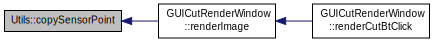
\includegraphics[width=350pt]{namespaceUtils_adc0438a85ca31977c95f5d27090d5346_icgraph}
\end{center}
\end{figure}


\hypertarget{namespaceUtils_a233ff9a0b34b10195a434f1ff66323b8}{\index{Utils@{Utils}!floattowxstr@{floattowxstr}}
\index{floattowxstr@{floattowxstr}!Utils@{Utils}}
\subsubsection[{floattowxstr}]{\setlength{\rightskip}{0pt plus 5cm}wx\-String Utils\-::floattowxstr (
\begin{DoxyParamCaption}
\item[{double}]{val}
\end{DoxyParamCaption}
)}}\label{namespaceUtils_a233ff9a0b34b10195a434f1ff66323b8}


Wandelt eine Fließkommazahl in einen wx\-Widgets-\/\-String um. 


\begin{DoxyParams}{Parameter}
{\em val} & Die umzuwandelnde Zahl. \\
\hline
\end{DoxyParams}
\begin{DoxyReturn}{Rückgabe}
Der entstandene String. 
\end{DoxyReturn}


Definiert in Zeile 36 der Datei utils.\-cpp.



Hier ist ein Graph der zeigt, wo diese Funktion aufgerufen wird\-:\nopagebreak
\begin{figure}[H]
\begin{center}
\leavevmode
\includegraphics[width=350pt]{namespaceUtils_a233ff9a0b34b10195a434f1ff66323b8_icgraph}
\end{center}
\end{figure}


\hypertarget{namespaceUtils_ac47160b3665d77f9e1a49a4045053add}{\index{Utils@{Utils}!floattowxstr@{floattowxstr}}
\index{floattowxstr@{floattowxstr}!Utils@{Utils}}
\subsubsection[{floattowxstr}]{\setlength{\rightskip}{0pt plus 5cm}wx\-String Utils\-::floattowxstr (
\begin{DoxyParamCaption}
\item[{double}]{val, }
\item[{int}]{digits}
\end{DoxyParamCaption}
)}}\label{namespaceUtils_ac47160b3665d77f9e1a49a4045053add}


Wandelt eine Fließkommazahl in einen wx\-Widgets-\/\-String um. 


\begin{DoxyParams}{Parameter}
{\em val} & Die umzuwandelnde Zahl. \\
\hline
{\em digits} & Anzahl der zu übernehmenden Stellen. \\
\hline
\end{DoxyParams}
\begin{DoxyReturn}{Rückgabe}
Der entstandene String. 
\end{DoxyReturn}


Definiert in Zeile 41 der Datei utils.\-cpp.

\hypertarget{namespaceUtils_a6a0ae18a42e2d206bc1b43da27820fe2}{\index{Utils@{Utils}!get\-Point\-Value@{get\-Point\-Value}}
\index{get\-Point\-Value@{get\-Point\-Value}!Utils@{Utils}}
\subsubsection[{get\-Point\-Value}]{\setlength{\rightskip}{0pt plus 5cm}double Utils\-::get\-Point\-Value (
\begin{DoxyParamCaption}
\item[{int \&}]{status, }
\item[{vector$<$ Sensor\-Point $>$ $\ast$}]{sensorpoints, }
\item[{double $\ast$}]{p, }
\item[{{\bf Interpolator} $\ast$}]{interpolator, }
\item[{vector$<$ Sensor\-Point $\ast$ $>$ $\ast$}]{prev\-\_\-tet = {\ttfamily NULL}, }
\item[{vector$<$ Sensor\-Point $\ast$ $>$ $\ast$}]{current\-\_\-tet = {\ttfamily NULL}}
\end{DoxyParamCaption}
)}}\label{namespaceUtils_a6a0ae18a42e2d206bc1b43da27820fe2}


Gibt den inter/extrapolierten Wert eines Punktes zurück. 


\begin{DoxyParams}{Parameter}
{\em status} & Rückgabevariable. 1\-: Punkt wurde extrapoliert 0\-: Punkt wurde interpoliert. -\/1\-: Alle Sensorpunkte sind komplanar. \\
\hline
{\em sensorpoints} & Die zu verwendenden Senosorpunkte. \\
\hline
{\em p} & Die Koordinaten des gesuchten Punktes. \\
\hline
{\em interpolator} & Das zu verwendende Interpolatorobjekt. \\
\hline
{\em prev\-\_\-tet} & Zuerst zu Testender Tetraeder (optional, N\-U\-L\-L zum Nichtverwenden). \\
\hline
{\em current\-\_\-tet} & Rückgabevariable für den zuletzt verwendeten Tetraeder (optional, N\-U\-L\-L zum Nichtverwenden). \\
\hline
\end{DoxyParams}
\begin{DoxyReturn}{Rückgabe}
Temperatur des gesuchten Punktes. 
\end{DoxyReturn}


Definiert in Zeile 258 der Datei utils.\-cpp.



Hier ist ein Graph, der zeigt, was diese Funktion aufruft\-:
\nopagebreak
\begin{figure}[H]
\begin{center}
\leavevmode
\includegraphics[width=350pt]{namespaceUtils_a6a0ae18a42e2d206bc1b43da27820fe2_cgraph}
\end{center}
\end{figure}




Hier ist ein Graph der zeigt, wo diese Funktion aufgerufen wird\-:
\nopagebreak
\begin{figure}[H]
\begin{center}
\leavevmode
\includegraphics[width=350pt]{namespaceUtils_a6a0ae18a42e2d206bc1b43da27820fe2_icgraph}
\end{center}
\end{figure}


\hypertarget{namespaceUtils_a5d6523eb946892eee52c9c74efd016de}{\index{Utils@{Utils}!hsv\-To\-Rgb@{hsv\-To\-Rgb}}
\index{hsv\-To\-Rgb@{hsv\-To\-Rgb}!Utils@{Utils}}
\subsubsection[{hsv\-To\-Rgb}]{\setlength{\rightskip}{0pt plus 5cm}float $\ast$ Utils\-::hsv\-To\-Rgb (
\begin{DoxyParamCaption}
\item[{float}]{h, }
\item[{float}]{s, }
\item[{float}]{v}
\end{DoxyParamCaption}
)}}\label{namespaceUtils_a5d6523eb946892eee52c9c74efd016de}


Wandelt eine Farbe im H\-S\-V-\/\-Format ins R\-G\-B-\/\-Format um. 


\begin{DoxyParams}{Parameter}
{\em h} & H-\/\-Komponente der Farbe. \\
\hline
{\em s} & S-\/\-Komponente der Farbe. \\
\hline
{\em v} & V-\/\-Komponente der Farbe. \\
\hline
\end{DoxyParams}
\begin{DoxyReturn}{Rückgabe}
R\-G\-B-\/\-Farbe als Liste mit 3 Werten im Bereich 0..1. Muss manuell mit delete\mbox{[}\mbox{]} freigegeben werden! 
\end{DoxyReturn}


Definiert in Zeile 46 der Datei utils.\-cpp.



Hier ist ein Graph der zeigt, wo diese Funktion aufgerufen wird\-:
\nopagebreak
\begin{figure}[H]
\begin{center}
\leavevmode
\includegraphics[width=350pt]{namespaceUtils_a5d6523eb946892eee52c9c74efd016de_icgraph}
\end{center}
\end{figure}


\hypertarget{namespaceUtils_af4ba26e928c7cef5269c51bfac49d547}{\index{Utils@{Utils}!next\-Combination@{next\-Combination}}
\index{next\-Combination@{next\-Combination}!Utils@{Utils}}
\subsubsection[{next\-Combination}]{\setlength{\rightskip}{0pt plus 5cm}void Utils\-::next\-Combination (
\begin{DoxyParamCaption}
\item[{vector$<$ int $>$ $\ast$}]{indices, }
\item[{int}]{depth, }
\item[{int}]{data\-Point\-Count}
\end{DoxyParamCaption}
)}}\label{namespaceUtils_af4ba26e928c7cef5269c51bfac49d547}


Ermöglicht das generieren aller möglichen Verteilungen von depth+1 Elementen auf data\-Point\-Count Plätze. 

Die Indices der Plätze, die die Elemente jeweils besetzten stehen in indices. Diese Funktion generiert aus der vorherigen Anordnung die Nächste. 
\begin{DoxyParams}{Parameter}
{\em indices} & Liste der Indices der Elemente. \\
\hline
{\em depth} & Anzahl der Elemente-\/1. \\
\hline
{\em data\-Point\-Count} & Anzahl der Plätze. \\
\hline
\end{DoxyParams}


Definiert in Zeile 13 der Datei utils.\-cpp.



Hier ist ein Graph der zeigt, wo diese Funktion aufgerufen wird\-:
\nopagebreak
\begin{figure}[H]
\begin{center}
\leavevmode
\includegraphics[width=350pt]{namespaceUtils_af4ba26e928c7cef5269c51bfac49d547_icgraph}
\end{center}
\end{figure}


\hypertarget{namespaceUtils_af8fc5d6dab27f759ab5d76757a53023f}{\index{Utils@{Utils}!point\-Inside\-Mesh@{point\-Inside\-Mesh}}
\index{point\-Inside\-Mesh@{point\-Inside\-Mesh}!Utils@{Utils}}
\subsubsection[{point\-Inside\-Mesh}]{\setlength{\rightskip}{0pt plus 5cm}int Utils\-::point\-Inside\-Mesh (
\begin{DoxyParamCaption}
\item[{{\bf Vector3\-D} $\ast$}]{p, }
\item[{tetgenio $\ast$}]{io, }
\item[{P\-I\-M\-\_\-algorithm}]{algorithm}
\end{DoxyParamCaption}
)}}\label{namespaceUtils_af8fc5d6dab27f759ab5d76757a53023f}


Testet, ob sich ein Punkt innerhalb eines Körpers befindet. 


\begin{DoxyParams}{Parameter}
{\em p} & Der zu testende Punkt. \\
\hline
{\em io} & Der zu testende Körper als Tetgen-\/\-Daten (s. Tetgen Dokumentation). \\
\hline
{\em algorithm} & Der zu verwendende Testalgorithmus (Empfohlen und ausschließlich verwendet\-: A\-L\-G\-O\-R\-I\-T\-H\-M\-\_\-\-T\-E\-T\-R\-A\-H\-E\-D\-R\-O\-N\-S). \\
\hline
\end{DoxyParams}
\begin{DoxyReturn}{Rückgabe}
1 Wenn innerhalb, 0 wenn außerhalb. Bei einer falschen Algorithmuskonstante -\/1. 
\end{DoxyReturn}


Definiert in Zeile 139 der Datei utils.\-cpp.



Hier ist ein Graph, der zeigt, was diese Funktion aufruft\-:\nopagebreak
\begin{figure}[H]
\begin{center}
\leavevmode
\includegraphics[width=350pt]{namespaceUtils_af8fc5d6dab27f759ab5d76757a53023f_cgraph}
\end{center}
\end{figure}




Hier ist ein Graph der zeigt, wo diese Funktion aufgerufen wird\-:
\nopagebreak
\begin{figure}[H]
\begin{center}
\leavevmode
\includegraphics[width=350pt]{namespaceUtils_af8fc5d6dab27f759ab5d76757a53023f_icgraph}
\end{center}
\end{figure}


\hypertarget{namespaceUtils_a9b995a1220a78be108b19bda4b776332}{\index{Utils@{Utils}!point\-Inside\-Tetrahedron@{point\-Inside\-Tetrahedron}}
\index{point\-Inside\-Tetrahedron@{point\-Inside\-Tetrahedron}!Utils@{Utils}}
\subsubsection[{point\-Inside\-Tetrahedron}]{\setlength{\rightskip}{0pt plus 5cm}int Utils\-::point\-Inside\-Tetrahedron (
\begin{DoxyParamCaption}
\item[{{\bf Vector3\-D} $\ast$}]{pges, }
\item[{{\bf Vector3\-D} $\ast$}]{v1, }
\item[{{\bf Vector3\-D} $\ast$}]{v2, }
\item[{{\bf Vector3\-D} $\ast$}]{v3, }
\item[{{\bf Vector3\-D} $\ast$}]{v4}
\end{DoxyParamCaption}
)}}\label{namespaceUtils_a9b995a1220a78be108b19bda4b776332}


Testet, ob sich ein Punkt innerhalb eines Tetraeders befindet. 


\begin{DoxyParams}{Parameter}
{\em pges} & Der zu testende Punkt. \\
\hline
{\em v1} & Der 1. Punkt des Tetraeders. \\
\hline
{\em v2} & Der 2. Punkt des Tetraeders. \\
\hline
{\em v3} & Der 3. Punkt des Tetraeders. \\
\hline
{\em v4} & Der 4. Punkt des Tetraeders. \\
\hline
\end{DoxyParams}
\begin{DoxyReturn}{Rückgabe}
1 Wenn innerhalb, 0 wenn außerhalb. -\/1, wenn der Tetraeder Komplanar ist. 
\end{DoxyReturn}


Definiert in Zeile 188 der Datei utils.\-cpp.



Hier ist ein Graph, der zeigt, was diese Funktion aufruft\-:\nopagebreak
\begin{figure}[H]
\begin{center}
\leavevmode
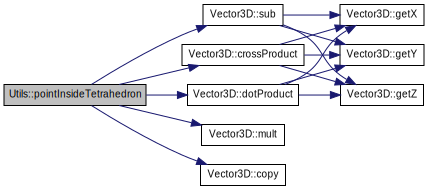
\includegraphics[width=350pt]{namespaceUtils_a9b995a1220a78be108b19bda4b776332_cgraph}
\end{center}
\end{figure}




Hier ist ein Graph der zeigt, wo diese Funktion aufgerufen wird\-:
\nopagebreak
\begin{figure}[H]
\begin{center}
\leavevmode
\includegraphics[width=350pt]{namespaceUtils_a9b995a1220a78be108b19bda4b776332_icgraph}
\end{center}
\end{figure}


\hypertarget{namespaceUtils_a8f7379e1915d2a04907eb9d99d0a56ad}{\index{Utils@{Utils}!point\-Inside\-Tetrahedron@{point\-Inside\-Tetrahedron}}
\index{point\-Inside\-Tetrahedron@{point\-Inside\-Tetrahedron}!Utils@{Utils}}
\subsubsection[{point\-Inside\-Tetrahedron}]{\setlength{\rightskip}{0pt plus 5cm}int Utils\-::point\-Inside\-Tetrahedron (
\begin{DoxyParamCaption}
\item[{double $\ast$}]{pges, }
\item[{double $\ast$}]{v1, }
\item[{double $\ast$}]{v2, }
\item[{double $\ast$}]{v3, }
\item[{double $\ast$}]{v4}
\end{DoxyParamCaption}
)}}\label{namespaceUtils_a8f7379e1915d2a04907eb9d99d0a56ad}


Testet, ob sich ein Punkt innerhalb eines Tetraeders befindet. 


\begin{DoxyParams}{Parameter}
{\em pges} & Koordinaten des zu testenden Punktes. \\
\hline
{\em v1} & Koordinaten des 1. Punktes des Tetraeders. \\
\hline
{\em v2} & Koordinaten des 2. Punktes des Tetraeders. \\
\hline
{\em v3} & Koordinaten des 3. Punktes des Tetraeders. \\
\hline
{\em v4} & Koordinaten des 4. Punktes des Tetraeders. \\
\hline
\end{DoxyParams}
\begin{DoxyReturn}{Rückgabe}
1 Wenn innerhalb, 0 wenn außerhalb. -\/1, wenn der Tetraeder Komplanar ist. 
\end{DoxyReturn}


Definiert in Zeile 250 der Datei utils.\-cpp.



Hier ist ein Graph, der zeigt, was diese Funktion aufruft\-:\nopagebreak
\begin{figure}[H]
\begin{center}
\leavevmode
\includegraphics[width=350pt]{namespaceUtils_a8f7379e1915d2a04907eb9d99d0a56ad_cgraph}
\end{center}
\end{figure}


\hypertarget{namespaceUtils_a40eaef4d22da849a5deb2f1153d88bbc}{\index{Utils@{Utils}!point\-Inside\-Tetrahedron@{point\-Inside\-Tetrahedron}}
\index{point\-Inside\-Tetrahedron@{point\-Inside\-Tetrahedron}!Utils@{Utils}}
\subsubsection[{point\-Inside\-Tetrahedron}]{\setlength{\rightskip}{0pt plus 5cm}int Utils\-::point\-Inside\-Tetrahedron (
\begin{DoxyParamCaption}
\item[{double $\ast$}]{p, }
\item[{vector$<$ Sensor\-Point $\ast$ $>$ $\ast$}]{tet}
\end{DoxyParamCaption}
)}}\label{namespaceUtils_a40eaef4d22da849a5deb2f1153d88bbc}


Testet, ob sich ein Punkt innerhalb eines Tetraeders befindet. 


\begin{DoxyParams}{Parameter}
{\em p} & Koordinaten des zu testenden Punktes. \\
\hline
{\em tet} & Der zu untersuchende Tetraeder als Liste von Sensordaten. \\
\hline
\end{DoxyParams}
\begin{DoxyReturn}{Rückgabe}
1 Wenn innerhalb, 0 wenn außerhalb. -\/1, wenn der Tetraeder Komplanar ist. 
\end{DoxyReturn}


Definiert in Zeile 242 der Datei utils.\-cpp.



Hier ist ein Graph, der zeigt, was diese Funktion aufruft\-:\nopagebreak
\begin{figure}[H]
\begin{center}
\leavevmode
\includegraphics[width=350pt]{namespaceUtils_a40eaef4d22da849a5deb2f1153d88bbc_cgraph}
\end{center}
\end{figure}


\hypertarget{namespaceUtils_a5f216cc7011a901130db81321b565334}{\index{Utils@{Utils}!ray\-Intersects\-Triangle@{ray\-Intersects\-Triangle}}
\index{ray\-Intersects\-Triangle@{ray\-Intersects\-Triangle}!Utils@{Utils}}
\subsubsection[{ray\-Intersects\-Triangle}]{\setlength{\rightskip}{0pt plus 5cm}int Utils\-::ray\-Intersects\-Triangle (
\begin{DoxyParamCaption}
\item[{{\bf Vector3\-D} $\ast$}]{p, }
\item[{{\bf Vector3\-D} $\ast$}]{direction, }
\item[{{\bf Triangle} $\ast$}]{tri, }
\item[{double $\ast$}]{depth}
\end{DoxyParamCaption}
)}}\label{namespaceUtils_a5f216cc7011a901130db81321b565334}


Testet, ob ein Strahl ein Dreieck schneidet. 


\begin{DoxyParams}{Parameter}
{\em p} & Ortsvektor zum Ausganspunkt des Strahls. \\
\hline
{\em direction} & Richtung des Strahls. \\
\hline
{\em tri} & Das zu testende Dreieck. \\
\hline
{\em depth} & Ausgabevariablie, ein Maß für den Abstand von Ausganspunkt zu Schnittpunkt. \\
\hline
\end{DoxyParams}
\begin{DoxyReturn}{Rückgabe}
Gibt 1 zurück, wenn es einen Schnittpunkt gibt, ansonsten 0. 
\end{DoxyReturn}


Definiert in Zeile 77 der Datei utils.\-cpp.



Hier ist ein Graph, der zeigt, was diese Funktion aufruft\-:\nopagebreak
\begin{figure}[H]
\begin{center}
\leavevmode
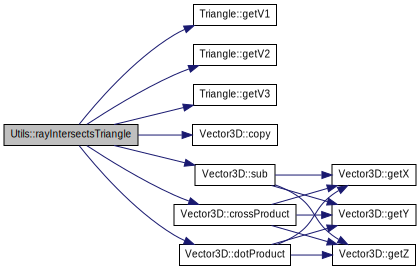
\includegraphics[width=350pt]{namespaceUtils_a5f216cc7011a901130db81321b565334_cgraph}
\end{center}
\end{figure}




Hier ist ein Graph der zeigt, wo diese Funktion aufgerufen wird\-:
\nopagebreak
\begin{figure}[H]
\begin{center}
\leavevmode
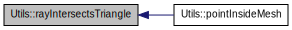
\includegraphics[width=350pt]{namespaceUtils_a5f216cc7011a901130db81321b565334_icgraph}
\end{center}
\end{figure}


\hypertarget{namespaceUtils_afac34330dde6235ee7395a4fd412ae0d}{\index{Utils@{Utils}!sqr@{sqr}}
\index{sqr@{sqr}!Utils@{Utils}}
\subsubsection[{sqr}]{\setlength{\rightskip}{0pt plus 5cm}double Utils\-::sqr (
\begin{DoxyParamCaption}
\item[{double}]{d}
\end{DoxyParamCaption}
)\hspace{0.3cm}{\ttfamily [inline]}}}\label{namespaceUtils_afac34330dde6235ee7395a4fd412ae0d}


Quadriert eine Zahl. 


\begin{DoxyParams}{Parameter}
{\em d} & Die zu quadrierende Zahl. \\
\hline
\end{DoxyParams}
\begin{DoxyReturn}{Rückgabe}
$d^2$. 
\end{DoxyReturn}


Definiert in Zeile 40 der Datei utils.\-h.


\chapter{Klassen-\/\-Dokumentation}
\hypertarget{classAnalyzer}{\section{Analyzer Klassenreferenz}
\label{classAnalyzer}\index{Analyzer@{Analyzer}}
}


Ermittelt Daten aus der Temperaturverteilung.  




{\ttfamily \#include $<$Analyzer.\-h$>$}

\subsection*{Klassen}
\begin{DoxyCompactItemize}
\item 
struct \hyperlink{structAnalyzer_1_1AnalyzerData__dataset}{Analyzer\-Data\-\_\-dataset}
\begin{DoxyCompactList}\small\item\em Analyseergebnisse für einen Sensordatensatz. \end{DoxyCompactList}\item 
struct \hyperlink{structAnalyzer_1_1AnalyzerData__material}{Analyzer\-Data\-\_\-material}
\begin{DoxyCompactList}\small\item\em Analyseergebnisse für ein Material. \end{DoxyCompactList}\item 
struct \hyperlink{structAnalyzer_1_1AnalyzerData__object}{Analyzer\-Data\-\_\-object}
\begin{DoxyCompactList}\small\item\em Analyseergebnisse für ein Objekt. \end{DoxyCompactList}\item 
struct \hyperlink{structAnalyzer_1_1AnalyzerData__point}{Analyzer\-Data\-\_\-point}
\begin{DoxyCompactList}\small\item\em Analyseergebnisse für einen Punkt. \end{DoxyCompactList}\end{DoxyCompactItemize}
\subsection*{Öffentliche Methoden}
\begin{DoxyCompactItemize}
\item 
\hyperlink{classAnalyzer_a1be2ff17bba265bdef6e1b44748eaf96}{Analyzer} ()
\begin{DoxyCompactList}\small\item\em Der Konstruktor. \end{DoxyCompactList}\item 
void \hyperlink{classAnalyzer_a2a7b5f169f664ccd9f206e508cba78ef}{analyze\-Object} (\hyperlink{classObjectData}{Object\-Data} $\ast$obj, \hyperlink{structAnalyzer_1_1AnalyzerData__object}{Analyzer\-Data\-\_\-object} $\ast$out, bool use\-\_\-markers=true, int sdindex=-\/1)
\begin{DoxyCompactList}\small\item\em Ermittelt Daten für ein Objekt. \end{DoxyCompactList}\item 
void \hyperlink{classAnalyzer_a8f73ee0aa71ae395a74b43dc76b35458}{analyze\-Point} (\hyperlink{classObjectData}{Object\-Data} $\ast$obj, \hyperlink{classVector3D}{Vector3\-D} $\ast$point, \hyperlink{structAnalyzer_1_1AnalyzerData__point}{Analyzer\-Data\-\_\-point} $\ast$point\-\_\-data, \hyperlink{classInterpolator}{Interpolator} $\ast$interpolator)
\begin{DoxyCompactList}\small\item\em Ermittelt Daten für einen Punkt am aktuell ausgewählten Zeitpunkt. \end{DoxyCompactList}\item 
virtual \hyperlink{classAnalyzer_afa899ac3a6aabbe59f791f69368ad740}{$\sim$\-Analyzer} ()
\begin{DoxyCompactList}\small\item\em Der Destruktor. \end{DoxyCompactList}\end{DoxyCompactItemize}
\subsection*{Freundbeziehungen}
\begin{DoxyCompactItemize}
\item 
std\-::ostream \& \hyperlink{classAnalyzer_a031acd0d5f2a8c997c18645dd548dca7}{operator$<$$<$} (std\-::ostream \&out, const \hyperlink{structAnalyzer_1_1AnalyzerData__object}{Analyzer\-Data\-\_\-object} \&data)
\begin{DoxyCompactList}\small\item\em Operator zum Ausgeben der Analysedaten für ein Objekt im cout-\/\-Stream. \end{DoxyCompactList}\end{DoxyCompactItemize}


\subsection{Ausführliche Beschreibung}
Ermittelt Daten aus der Temperaturverteilung. 

Definiert in Zeile 21 der Datei Analyzer.\-h.



\subsection{Beschreibung der Konstruktoren und Destruktoren}
\hypertarget{classAnalyzer_a1be2ff17bba265bdef6e1b44748eaf96}{\index{Analyzer@{Analyzer}!Analyzer@{Analyzer}}
\index{Analyzer@{Analyzer}!Analyzer@{Analyzer}}
\subsubsection[{Analyzer}]{\setlength{\rightskip}{0pt plus 5cm}Analyzer\-::\-Analyzer (
\begin{DoxyParamCaption}
{}
\end{DoxyParamCaption}
)}}\label{classAnalyzer_a1be2ff17bba265bdef6e1b44748eaf96}


Der Konstruktor. 



Definiert in Zeile 14 der Datei Analyzer.\-cpp.

\hypertarget{classAnalyzer_afa899ac3a6aabbe59f791f69368ad740}{\index{Analyzer@{Analyzer}!$\sim$\-Analyzer@{$\sim$\-Analyzer}}
\index{$\sim$\-Analyzer@{$\sim$\-Analyzer}!Analyzer@{Analyzer}}
\subsubsection[{$\sim$\-Analyzer}]{\setlength{\rightskip}{0pt plus 5cm}Analyzer\-::$\sim$\-Analyzer (
\begin{DoxyParamCaption}
{}
\end{DoxyParamCaption}
)\hspace{0.3cm}{\ttfamily [virtual]}}}\label{classAnalyzer_afa899ac3a6aabbe59f791f69368ad740}


Der Destruktor. 



Definiert in Zeile 108 der Datei Analyzer.\-cpp.



\subsection{Dokumentation der Elementfunktionen}
\hypertarget{classAnalyzer_a2a7b5f169f664ccd9f206e508cba78ef}{\index{Analyzer@{Analyzer}!analyze\-Object@{analyze\-Object}}
\index{analyze\-Object@{analyze\-Object}!Analyzer@{Analyzer}}
\subsubsection[{analyze\-Object}]{\setlength{\rightskip}{0pt plus 5cm}void Analyzer\-::analyze\-Object (
\begin{DoxyParamCaption}
\item[{{\bf Object\-Data} $\ast$}]{obj, }
\item[{{\bf Analyzer\-Data\-\_\-object} $\ast$}]{out, }
\item[{bool}]{use\-\_\-markers = {\ttfamily true}, }
\item[{int}]{sdindex = {\ttfamily -\/1}}
\end{DoxyParamCaption}
)}}\label{classAnalyzer_a2a7b5f169f664ccd9f206e508cba78ef}


Ermittelt Daten für ein Objekt. 


\begin{DoxyParams}{Parameter}
{\em obj} & Das zu analysierende Objekt. \\
\hline
{\em out} & Referenz auf die \hyperlink{structAnalyzer_1_1AnalyzerData__object}{Analyzer\-Data\-\_\-object} -\/\-Struktur in der die Analyseergebnisse gespeichert werden sollen. \\
\hline
{\em use\-\_\-markers} & Die markierten Zeitpunkte eines Sensordatensatzes analysieren. Wenn false wird nur der aktuell ausgewählte Zeitpunkt analysiert. \\
\hline
{\em sdindex} & Nur den Sensordatensatz mit diesem Index analysieren. \\
\hline
\end{DoxyParams}


Definiert in Zeile 18 der Datei Analyzer.\-cpp.



Hier ist ein Graph, der zeigt, was diese Funktion aufruft\-:
\nopagebreak
\begin{figure}[H]
\begin{center}
\leavevmode
\includegraphics[width=350pt]{classAnalyzer_a2a7b5f169f664ccd9f206e508cba78ef_cgraph}
\end{center}
\end{figure}




Hier ist ein Graph der zeigt, wo diese Funktion aufgerufen wird\-:\nopagebreak
\begin{figure}[H]
\begin{center}
\leavevmode
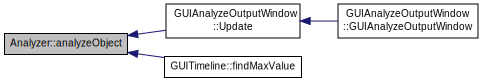
\includegraphics[width=350pt]{classAnalyzer_a2a7b5f169f664ccd9f206e508cba78ef_icgraph}
\end{center}
\end{figure}


\hypertarget{classAnalyzer_a8f73ee0aa71ae395a74b43dc76b35458}{\index{Analyzer@{Analyzer}!analyze\-Point@{analyze\-Point}}
\index{analyze\-Point@{analyze\-Point}!Analyzer@{Analyzer}}
\subsubsection[{analyze\-Point}]{\setlength{\rightskip}{0pt plus 5cm}void Analyzer\-::analyze\-Point (
\begin{DoxyParamCaption}
\item[{{\bf Object\-Data} $\ast$}]{obj, }
\item[{{\bf Vector3\-D} $\ast$}]{point, }
\item[{{\bf Analyzer\-Data\-\_\-point} $\ast$}]{point\-\_\-data, }
\item[{{\bf Interpolator} $\ast$}]{interpolator}
\end{DoxyParamCaption}
)}}\label{classAnalyzer_a8f73ee0aa71ae395a74b43dc76b35458}


Ermittelt Daten für einen Punkt am aktuell ausgewählten Zeitpunkt. 


\begin{DoxyParams}{Parameter}
{\em obj} & Das zu analysierende Objekt. \\
\hline
{\em point} & Der Ortsvektor zum zu analysierenden Punkt. \\
\hline
{\em point\-\_\-data} & Referenz auf die \hyperlink{structAnalyzer_1_1AnalyzerData__point}{Analyzer\-Data\-\_\-point} -\/\-Struktur in der die Analyseergebnisse gespeichert werden sollen. \\
\hline
{\em interpolator} & Das zu verwendende Interpolatorobjekt. \\
\hline
\end{DoxyParams}


Definiert in Zeile 83 der Datei Analyzer.\-cpp.



Hier ist ein Graph, der zeigt, was diese Funktion aufruft\-:
\nopagebreak
\begin{figure}[H]
\begin{center}
\leavevmode
\includegraphics[width=350pt]{classAnalyzer_a8f73ee0aa71ae395a74b43dc76b35458_cgraph}
\end{center}
\end{figure}




Hier ist ein Graph der zeigt, wo diese Funktion aufgerufen wird\-:\nopagebreak
\begin{figure}[H]
\begin{center}
\leavevmode
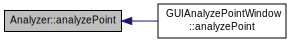
\includegraphics[width=350pt]{classAnalyzer_a8f73ee0aa71ae395a74b43dc76b35458_icgraph}
\end{center}
\end{figure}




\subsection{Freundbeziehungen und Funktionsdokumentation}
\hypertarget{classAnalyzer_a031acd0d5f2a8c997c18645dd548dca7}{\index{Analyzer@{Analyzer}!operator$<$$<$@{operator$<$$<$}}
\index{operator$<$$<$@{operator$<$$<$}!Analyzer@{Analyzer}}
\subsubsection[{operator$<$$<$}]{\setlength{\rightskip}{0pt plus 5cm}std\-::ostream\& operator$<$$<$ (
\begin{DoxyParamCaption}
\item[{std\-::ostream \&}]{out, }
\item[{const {\bf Analyzer\-Data\-\_\-object} \&}]{data}
\end{DoxyParamCaption}
)\hspace{0.3cm}{\ttfamily [friend]}}}\label{classAnalyzer_a031acd0d5f2a8c997c18645dd548dca7}


Operator zum Ausgeben der Analysedaten für ein Objekt im cout-\/\-Stream. 



Definiert in Zeile 91 der Datei Analyzer.\-cpp.



Die Dokumentation für diese Klasse wurde erzeugt aufgrund der Dateien\-:\begin{DoxyCompactItemize}
\item 
simpleanalyzer-\/gui/src/processing/\hyperlink{Analyzer_8h}{Analyzer.\-h}\item 
simpleanalyzer-\/gui/src/processing/\hyperlink{Analyzer_8cpp}{Analyzer.\-cpp}\end{DoxyCompactItemize}

\hypertarget{structAnalyzer_1_1AnalyzerData__dataset}{\section{Analyzer\-:\-:Analyzer\-Data\-\_\-dataset Strukturreferenz}
\label{structAnalyzer_1_1AnalyzerData__dataset}\index{Analyzer\-::\-Analyzer\-Data\-\_\-dataset@{Analyzer\-::\-Analyzer\-Data\-\_\-dataset}}
}


Analyseergebnisse für einen Sensordatensatz.  




{\ttfamily \#include $<$Analyzer.\-h$>$}



Zusammengehörigkeiten von Analyzer\-:\-:Analyzer\-Data\-\_\-dataset\-:
\nopagebreak
\begin{figure}[H]
\begin{center}
\leavevmode
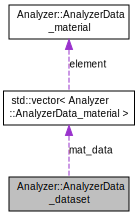
\includegraphics[width=210pt]{structAnalyzer_1_1AnalyzerData__dataset__coll__graph}
\end{center}
\end{figure}
\subsection*{Öffentliche Attribute}
\begin{DoxyCompactItemize}
\item 
string \hyperlink{structAnalyzer_1_1AnalyzerData__dataset_a53f3c1896123de4dc00f01e593d5f70d}{name}
\begin{DoxyCompactList}\small\item\em Der Name des Sensordatensatzes$<$. \end{DoxyCompactList}\item 
double \hyperlink{structAnalyzer_1_1AnalyzerData__dataset_aaefb798e2611790d5d956fe597bbafe0}{heat\-\_\-energy}
\begin{DoxyCompactList}\small\item\em Die Wärmeenergie, die das Objekt für diesen Datensatz enthält. \end{DoxyCompactList}\item 
\hyperlink{classstd_1_1vector}{vector}$<$ \hyperlink{structAnalyzer_1_1AnalyzerData__material}{Analyzer\-Data\-\_\-material} $>$ \hyperlink{structAnalyzer_1_1AnalyzerData__dataset_a25d0189c93bc0da58f778750edb2a2b9}{mat\-\_\-data}
\begin{DoxyCompactList}\small\item\em Die Analyseergebnisse für die Einzelnen Materialien. \end{DoxyCompactList}\end{DoxyCompactItemize}


\subsection{Ausführliche Beschreibung}
Analyseergebnisse für einen Sensordatensatz. 

Definiert in Zeile 35 der Datei Analyzer.\-h.



\subsection{Dokumentation der Datenelemente}
\hypertarget{structAnalyzer_1_1AnalyzerData__dataset_aaefb798e2611790d5d956fe597bbafe0}{\index{Analyzer\-::\-Analyzer\-Data\-\_\-dataset@{Analyzer\-::\-Analyzer\-Data\-\_\-dataset}!heat\-\_\-energy@{heat\-\_\-energy}}
\index{heat\-\_\-energy@{heat\-\_\-energy}!Analyzer::AnalyzerData_dataset@{Analyzer\-::\-Analyzer\-Data\-\_\-dataset}}
\subsubsection[{heat\-\_\-energy}]{\setlength{\rightskip}{0pt plus 5cm}double Analyzer\-::\-Analyzer\-Data\-\_\-dataset\-::heat\-\_\-energy}}\label{structAnalyzer_1_1AnalyzerData__dataset_aaefb798e2611790d5d956fe597bbafe0}


Die Wärmeenergie, die das Objekt für diesen Datensatz enthält. 



Definiert in Zeile 37 der Datei Analyzer.\-h.

\hypertarget{structAnalyzer_1_1AnalyzerData__dataset_a25d0189c93bc0da58f778750edb2a2b9}{\index{Analyzer\-::\-Analyzer\-Data\-\_\-dataset@{Analyzer\-::\-Analyzer\-Data\-\_\-dataset}!mat\-\_\-data@{mat\-\_\-data}}
\index{mat\-\_\-data@{mat\-\_\-data}!Analyzer::AnalyzerData_dataset@{Analyzer\-::\-Analyzer\-Data\-\_\-dataset}}
\subsubsection[{mat\-\_\-data}]{\setlength{\rightskip}{0pt plus 5cm}{\bf vector}$<${\bf Analyzer\-Data\-\_\-material}$>$ Analyzer\-::\-Analyzer\-Data\-\_\-dataset\-::mat\-\_\-data}}\label{structAnalyzer_1_1AnalyzerData__dataset_a25d0189c93bc0da58f778750edb2a2b9}


Die Analyseergebnisse für die Einzelnen Materialien. 



Definiert in Zeile 38 der Datei Analyzer.\-h.

\hypertarget{structAnalyzer_1_1AnalyzerData__dataset_a53f3c1896123de4dc00f01e593d5f70d}{\index{Analyzer\-::\-Analyzer\-Data\-\_\-dataset@{Analyzer\-::\-Analyzer\-Data\-\_\-dataset}!name@{name}}
\index{name@{name}!Analyzer::AnalyzerData_dataset@{Analyzer\-::\-Analyzer\-Data\-\_\-dataset}}
\subsubsection[{name}]{\setlength{\rightskip}{0pt plus 5cm}string Analyzer\-::\-Analyzer\-Data\-\_\-dataset\-::name}}\label{structAnalyzer_1_1AnalyzerData__dataset_a53f3c1896123de4dc00f01e593d5f70d}


Der Name des Sensordatensatzes$<$. 



Definiert in Zeile 36 der Datei Analyzer.\-h.



Die Dokumentation für diese Struktur wurde erzeugt aufgrund der Datei\-:\begin{DoxyCompactItemize}
\item 
/daten/\-Projekte/eclipse\-\_\-workspace/simpleanalyzer-\/gui/src/processing/\hyperlink{Analyzer_8h}{Analyzer.\-h}\end{DoxyCompactItemize}

\hypertarget{structAnalyzer_1_1AnalyzerData__material}{\section{Analyzer\-:\-:Analyzer\-Data\-\_\-material Strukturreferenz}
\label{structAnalyzer_1_1AnalyzerData__material}\index{Analyzer\-::\-Analyzer\-Data\-\_\-material@{Analyzer\-::\-Analyzer\-Data\-\_\-material}}
}


Analyseergebnisse für ein Material.  




{\ttfamily \#include $<$Analyzer.\-h$>$}

\subsection*{Öffentliche Attribute}
\begin{DoxyCompactItemize}
\item 
string \hyperlink{structAnalyzer_1_1AnalyzerData__material_a0a6b01fc900ce677ae8403d3a85b829b}{name}
\begin{DoxyCompactList}\small\item\em Der Name des Material. \end{DoxyCompactList}\item 
double \hyperlink{structAnalyzer_1_1AnalyzerData__material_a20017730ff899b65f91aa30caaf35dd6}{volume}
\begin{DoxyCompactList}\small\item\em Das Volumen, das dem Material zugeordnet ist. \end{DoxyCompactList}\item 
double \hyperlink{structAnalyzer_1_1AnalyzerData__material_a94efc7f38f7f59c97a48a0155f9c4719}{heat\-\_\-energy}
\begin{DoxyCompactList}\small\item\em Die Wärmeenergie, die das dem Material zugeordnete Volumen enthält. \end{DoxyCompactList}\end{DoxyCompactItemize}


\subsection{Ausführliche Beschreibung}
Analyseergebnisse für ein Material. 

Definiert in Zeile 26 der Datei Analyzer.\-h.



\subsection{Dokumentation der Datenelemente}
\hypertarget{structAnalyzer_1_1AnalyzerData__material_a94efc7f38f7f59c97a48a0155f9c4719}{\index{Analyzer\-::\-Analyzer\-Data\-\_\-material@{Analyzer\-::\-Analyzer\-Data\-\_\-material}!heat\-\_\-energy@{heat\-\_\-energy}}
\index{heat\-\_\-energy@{heat\-\_\-energy}!Analyzer::AnalyzerData_material@{Analyzer\-::\-Analyzer\-Data\-\_\-material}}
\subsubsection[{heat\-\_\-energy}]{\setlength{\rightskip}{0pt plus 5cm}double Analyzer\-::\-Analyzer\-Data\-\_\-material\-::heat\-\_\-energy}}\label{structAnalyzer_1_1AnalyzerData__material_a94efc7f38f7f59c97a48a0155f9c4719}


Die Wärmeenergie, die das dem Material zugeordnete Volumen enthält. 

$<$ 

Definiert in Zeile 29 der Datei Analyzer.\-h.

\hypertarget{structAnalyzer_1_1AnalyzerData__material_a0a6b01fc900ce677ae8403d3a85b829b}{\index{Analyzer\-::\-Analyzer\-Data\-\_\-material@{Analyzer\-::\-Analyzer\-Data\-\_\-material}!name@{name}}
\index{name@{name}!Analyzer::AnalyzerData_material@{Analyzer\-::\-Analyzer\-Data\-\_\-material}}
\subsubsection[{name}]{\setlength{\rightskip}{0pt plus 5cm}string Analyzer\-::\-Analyzer\-Data\-\_\-material\-::name}}\label{structAnalyzer_1_1AnalyzerData__material_a0a6b01fc900ce677ae8403d3a85b829b}


Der Name des Material. 

$<$ 

Definiert in Zeile 27 der Datei Analyzer.\-h.

\hypertarget{structAnalyzer_1_1AnalyzerData__material_a20017730ff899b65f91aa30caaf35dd6}{\index{Analyzer\-::\-Analyzer\-Data\-\_\-material@{Analyzer\-::\-Analyzer\-Data\-\_\-material}!volume@{volume}}
\index{volume@{volume}!Analyzer::AnalyzerData_material@{Analyzer\-::\-Analyzer\-Data\-\_\-material}}
\subsubsection[{volume}]{\setlength{\rightskip}{0pt plus 5cm}double Analyzer\-::\-Analyzer\-Data\-\_\-material\-::volume}}\label{structAnalyzer_1_1AnalyzerData__material_a20017730ff899b65f91aa30caaf35dd6}


Das Volumen, das dem Material zugeordnet ist. 

$<$ 

Definiert in Zeile 28 der Datei Analyzer.\-h.



Die Dokumentation für diese Struktur wurde erzeugt aufgrund der Datei\-:\begin{DoxyCompactItemize}
\item 
/daten/\-Projekte/eclipse\-\_\-workspace/simpleanalyzer-\/gui/src/processing/\hyperlink{Analyzer_8h}{Analyzer.\-h}\end{DoxyCompactItemize}

\hypertarget{structAnalyzer_1_1AnalyzerData__object}{\section{Analyzer\-:\-:Analyzer\-Data\-\_\-object Strukturreferenz}
\label{structAnalyzer_1_1AnalyzerData__object}\index{Analyzer\-::\-Analyzer\-Data\-\_\-object@{Analyzer\-::\-Analyzer\-Data\-\_\-object}}
}


Analyseergebnisse für ein Objekt.  




{\ttfamily \#include $<$Analyzer.\-h$>$}

\subsection*{Öffentliche Attribute}
\begin{DoxyCompactItemize}
\item 
double \hyperlink{structAnalyzer_1_1AnalyzerData__object_a78ddeb311ff702e110fc1d483d826920}{volume}
\begin{DoxyCompactList}\small\item\em Das Volumen des Objekts. \end{DoxyCompactList}\item 
vector$<$ \hyperlink{structAnalyzer_1_1AnalyzerData__dataset}{Analyzer\-Data\-\_\-dataset} $>$ \hyperlink{structAnalyzer_1_1AnalyzerData__object_a5d36dcf805f37b0e29134236e3881fca}{data\-\_\-sets}
\begin{DoxyCompactList}\small\item\em Die Analyseergebisse für die Sensordatensätze. \end{DoxyCompactList}\end{DoxyCompactItemize}


\subsection{Ausführliche Beschreibung}
Analyseergebnisse für ein Objekt. 

Definiert in Zeile 42 der Datei Analyzer.\-h.



\subsection{Dokumentation der Datenelemente}
\hypertarget{structAnalyzer_1_1AnalyzerData__object_a5d36dcf805f37b0e29134236e3881fca}{\index{Analyzer\-::\-Analyzer\-Data\-\_\-object@{Analyzer\-::\-Analyzer\-Data\-\_\-object}!data\-\_\-sets@{data\-\_\-sets}}
\index{data\-\_\-sets@{data\-\_\-sets}!Analyzer::AnalyzerData_object@{Analyzer\-::\-Analyzer\-Data\-\_\-object}}
\subsubsection[{data\-\_\-sets}]{\setlength{\rightskip}{0pt plus 5cm}vector$<${\bf Analyzer\-Data\-\_\-dataset}$>$ Analyzer\-::\-Analyzer\-Data\-\_\-object\-::data\-\_\-sets}}\label{structAnalyzer_1_1AnalyzerData__object_a5d36dcf805f37b0e29134236e3881fca}


Die Analyseergebisse für die Sensordatensätze. 

$<$ 

Definiert in Zeile 44 der Datei Analyzer.\-h.

\hypertarget{structAnalyzer_1_1AnalyzerData__object_a78ddeb311ff702e110fc1d483d826920}{\index{Analyzer\-::\-Analyzer\-Data\-\_\-object@{Analyzer\-::\-Analyzer\-Data\-\_\-object}!volume@{volume}}
\index{volume@{volume}!Analyzer::AnalyzerData_object@{Analyzer\-::\-Analyzer\-Data\-\_\-object}}
\subsubsection[{volume}]{\setlength{\rightskip}{0pt plus 5cm}double Analyzer\-::\-Analyzer\-Data\-\_\-object\-::volume}}\label{structAnalyzer_1_1AnalyzerData__object_a78ddeb311ff702e110fc1d483d826920}


Das Volumen des Objekts. 

$<$ 

Definiert in Zeile 43 der Datei Analyzer.\-h.



Die Dokumentation für diese Struktur wurde erzeugt aufgrund der Datei\-:\begin{DoxyCompactItemize}
\item 
simpleanalyzer-\/gui/src/processing/\hyperlink{Analyzer_8h}{Analyzer.\-h}\end{DoxyCompactItemize}

\hypertarget{structAnalyzer_1_1AnalyzerData__point}{\section{Analyzer\-:\-:Analyzer\-Data\-\_\-point Strukturreferenz}
\label{structAnalyzer_1_1AnalyzerData__point}\index{Analyzer\-::\-Analyzer\-Data\-\_\-point@{Analyzer\-::\-Analyzer\-Data\-\_\-point}}
}


Analyseergebnisse für einen Punkt.  




{\ttfamily \#include $<$Analyzer.\-h$>$}

\subsection*{Öffentliche Attribute}
\begin{DoxyCompactItemize}
\item 
double \hyperlink{structAnalyzer_1_1AnalyzerData__point_a150b00a3d0be5d1c75b39292d213cbfa}{value}
\begin{DoxyCompactList}\small\item\em Die Temperatur an diesem Punkt. \end{DoxyCompactList}\item 
bool \hyperlink{structAnalyzer_1_1AnalyzerData__point_af4d2c2bd41aebc3c243afc5544bed81a}{extrapolated}
\begin{DoxyCompactList}\small\item\em Ist der Punkt extrapoliert? \end{DoxyCompactList}\end{DoxyCompactItemize}


\subsection{Ausführliche Beschreibung}
Analyseergebnisse für einen Punkt. 

Definiert in Zeile 52 der Datei Analyzer.\-h.



\subsection{Dokumentation der Datenelemente}
\hypertarget{structAnalyzer_1_1AnalyzerData__point_af4d2c2bd41aebc3c243afc5544bed81a}{\index{Analyzer\-::\-Analyzer\-Data\-\_\-point@{Analyzer\-::\-Analyzer\-Data\-\_\-point}!extrapolated@{extrapolated}}
\index{extrapolated@{extrapolated}!Analyzer::AnalyzerData_point@{Analyzer\-::\-Analyzer\-Data\-\_\-point}}
\subsubsection[{extrapolated}]{\setlength{\rightskip}{0pt plus 5cm}bool Analyzer\-::\-Analyzer\-Data\-\_\-point\-::extrapolated}}\label{structAnalyzer_1_1AnalyzerData__point_af4d2c2bd41aebc3c243afc5544bed81a}


Ist der Punkt extrapoliert? 



Definiert in Zeile 54 der Datei Analyzer.\-h.

\hypertarget{structAnalyzer_1_1AnalyzerData__point_a150b00a3d0be5d1c75b39292d213cbfa}{\index{Analyzer\-::\-Analyzer\-Data\-\_\-point@{Analyzer\-::\-Analyzer\-Data\-\_\-point}!value@{value}}
\index{value@{value}!Analyzer::AnalyzerData_point@{Analyzer\-::\-Analyzer\-Data\-\_\-point}}
\subsubsection[{value}]{\setlength{\rightskip}{0pt plus 5cm}double Analyzer\-::\-Analyzer\-Data\-\_\-point\-::value}}\label{structAnalyzer_1_1AnalyzerData__point_a150b00a3d0be5d1c75b39292d213cbfa}


Die Temperatur an diesem Punkt. 



Definiert in Zeile 53 der Datei Analyzer.\-h.



Die Dokumentation für diese Struktur wurde erzeugt aufgrund der Datei\-:\begin{DoxyCompactItemize}
\item 
/daten/\-Projekte/eclipse\-\_\-workspace/simpleanalyzer-\/gui/src/processing/\hyperlink{Analyzer_8h}{Analyzer.\-h}\end{DoxyCompactItemize}

\hypertarget{classCsvToSdConverter}{\section{Csv\-To\-Sd\-Converter Klassenreferenz}
\label{classCsvToSdConverter}\index{Csv\-To\-Sd\-Converter@{Csv\-To\-Sd\-Converter}}
}


Konverter von .csv zu .tsd.  




Zusammengehörigkeiten von Csv\-To\-Sd\-Converter\-:\nopagebreak
\begin{figure}[H]
\begin{center}
\leavevmode
\includegraphics[width=220pt]{classCsvToSdConverter__coll__graph}
\end{center}
\end{figure}
\subsection*{Klassen}
\begin{DoxyCompactItemize}
\item 
struct \hyperlink{structCsvToSdConverter_1_1Options}{Options}
\begin{DoxyCompactList}\small\item\em Strunktur für die Programmeinstellungen. \end{DoxyCompactList}\end{DoxyCompactItemize}
\subsection*{Öffentliche Methoden}
\begin{DoxyCompactItemize}
\item 
int \hyperlink{classCsvToSdConverter_a226c1dfaf88433cc9edf6570798231ec}{convert} (int argc, char $\ast$argv\mbox{[}$\,$\mbox{]})
\begin{DoxyCompactList}\small\item\em Wandelt die Daten der .csv-\/\-Datei ein eine .tsd-\/\-Datei um. \end{DoxyCompactList}\end{DoxyCompactItemize}
\subsection*{Geschützte Methoden}
\begin{DoxyCompactItemize}
\item 
bool \hyperlink{classCsvToSdConverter_aee01d9654ddf4aac5660b64f39d136de}{contains} (\hyperlink{classstd_1_1vector}{std\-::vector}$<$ string $>$ \&Vec, const string \&Element)
\begin{DoxyCompactList}\small\item\em Testet, ob sich ein String in einer Liste von Strings befindet. \end{DoxyCompactList}\item 
bool \hyperlink{classCsvToSdConverter_a74e089d02b3e184de4784ad35dfb6f96}{contains} (\hyperlink{classstd_1_1vector}{std\-::vector}$<$ int $>$ \&Vec, const int \&Element)
\begin{DoxyCompactList}\small\item\em Testet, ob sich eine Ganzzahl in einer Liste von Ganzzahlen befindet. \end{DoxyCompactList}\item 
string \hyperlink{classCsvToSdConverter_a83da8c064200da09a028d457a53263c5}{get\-Text\-Block} (string data, int n)
\begin{DoxyCompactList}\small\item\em Gibt den n-\/ten durch Leerzeichen abgetrennten Block aus einem String zurück. \end{DoxyCompactList}\item 
void \hyperlink{classCsvToSdConverter_a4be5732a05287e3506925049ee990e1e}{parse\-Line} (string line, \hyperlink{classstd_1_1vector}{vector}$<$ string $>$ \&out, \hyperlink{classstd_1_1vector}{vector}$<$ string $>$ $\ast$timestamps, \hyperlink{classstd_1_1vector}{vector}$<$ string $>$ $\ast$names, \hyperlink{classstd_1_1vector}{vector}$<$ int $>$ $\ast$valid\-\_\-cols)
\begin{DoxyCompactList}\small\item\em Sammelt Daten aus einer Textzeile (string). \end{DoxyCompactList}\item 
void \hyperlink{classCsvToSdConverter_a16d31068591e8c70604267e34c0f0cb2}{replace\-All} (string \&str, const string from, const string to)
\begin{DoxyCompactList}\small\item\em Ersetzt in einem String alle Vorkommen eines Teilstrings durch einen Anderen. \end{DoxyCompactList}\item 
bool \hyperlink{classCsvToSdConverter_a6cfc076fd11f10d70767750a6aaf1f7c}{read\-Configuration} (string binary\-\_\-path)
\begin{DoxyCompactList}\small\item\em Liest und setzt die Programmkonfiguration aus der Konfigurationsdatei. \end{DoxyCompactList}\item 
bool \hyperlink{classCsvToSdConverter_aec2430ade6f76783c958d0b8466444c4}{read\-Sensor\-Definitions} (string path, \hyperlink{classstd_1_1vector}{vector}$<$ string $>$ $\ast$sensor\-\_\-names, \hyperlink{classstd_1_1vector}{vector}$<$ string $>$ $\ast$sensor\-\_\-data)
\begin{DoxyCompactList}\small\item\em Liest die Daten aus der Sensordefinitionsdatei. \end{DoxyCompactList}\item 
bool \hyperlink{classCsvToSdConverter_adae10f022f4f05195c2a4b0a620d4645}{parse\-Arguments} (int argc, char $\ast$argv\mbox{[}$\,$\mbox{]}, string \&sdef\-\_\-file, string \&input\-\_\-file, string \&output\-\_\-file)
\begin{DoxyCompactList}\small\item\em Wertet die Programmargumente aus. \end{DoxyCompactList}\item 
bool \hyperlink{classCsvToSdConverter_ae6a8febba248592df4a0d0588018b67c}{read\-Input\-File} (string path, \hyperlink{classstd_1_1vector}{vector}$<$ string $>$ \&sensor\-\_\-names, \hyperlink{classstd_1_1vector}{vector}$<$ \hyperlink{classstd_1_1vector}{vector}$<$ string $>$ $>$ \&values, \hyperlink{classstd_1_1vector}{vector}$<$ string $>$ \&timestamps, \hyperlink{classstd_1_1vector}{vector}$<$ string $>$ \&names)
\begin{DoxyCompactList}\small\item\em Liest die Daten aus der Eingabedatei. \end{DoxyCompactList}\item 
bool \hyperlink{classCsvToSdConverter_a5a1749027e2c4dbe00feecc55b823226}{write\-Output\-File} (string path, \hyperlink{classstd_1_1vector}{vector}$<$ string $>$ \&sensor\-\_\-names, \hyperlink{classstd_1_1vector}{vector}$<$ string $>$ \&sensor\-\_\-data, \hyperlink{classstd_1_1vector}{vector}$<$ \hyperlink{classstd_1_1vector}{vector}$<$ string $>$ $>$ \&values, \hyperlink{classstd_1_1vector}{vector}$<$ string $>$ \&timestamps, \hyperlink{classstd_1_1vector}{vector}$<$ string $>$ \&names)
\begin{DoxyCompactList}\small\item\em Schreibt die Ausgabedatei. \end{DoxyCompactList}\end{DoxyCompactItemize}
\subsection*{Geschützte Attribute}
\begin{DoxyCompactItemize}
\item 
string \hyperlink{classCsvToSdConverter_a185377b44506f75748a4d56bc372ee50}{configpaths} \mbox{[}\hyperlink{classCsvToSdConverter_ad2278682506407d3172e8fca834891fe}{N\-U\-M\-B\-E\-R\-O\-F\-P\-A\-T\-H\-S}\mbox{]}
\begin{DoxyCompactList}\small\item\em Suchpfade für die Konfigurationsdatei. \end{DoxyCompactList}\item 
struct \hyperlink{structCsvToSdConverter_1_1Options}{Csv\-To\-Sd\-Converter\-::\-Options} \hyperlink{classCsvToSdConverter_aed83889861a110c9913adb5b9f4d9eb3}{opts}
\begin{DoxyCompactList}\small\item\em Hält die verwendeten Programmeinstellungen. \end{DoxyCompactList}\end{DoxyCompactItemize}
\subsection*{Statische, geschützte Attribute}
\begin{DoxyCompactItemize}
\item 
static const int \hyperlink{classCsvToSdConverter_ad2278682506407d3172e8fca834891fe}{N\-U\-M\-B\-E\-R\-O\-F\-P\-A\-T\-H\-S} = 2
\begin{DoxyCompactList}\small\item\em Anzahl der Suchpfade für die Konfigurationsdatei. \end{DoxyCompactList}\end{DoxyCompactItemize}


\subsection{Ausführliche Beschreibung}
Konverter von .csv zu .tsd. 

Definiert in Zeile 19 der Datei main.\-cpp.



\subsection{Dokumentation der Elementfunktionen}
\hypertarget{classCsvToSdConverter_aee01d9654ddf4aac5660b64f39d136de}{\index{Csv\-To\-Sd\-Converter@{Csv\-To\-Sd\-Converter}!contains@{contains}}
\index{contains@{contains}!CsvToSdConverter@{Csv\-To\-Sd\-Converter}}
\subsubsection[{contains}]{\setlength{\rightskip}{0pt plus 5cm}bool Csv\-To\-Sd\-Converter\-::contains (
\begin{DoxyParamCaption}
\item[{{\bf std\-::vector}$<$ string $>$ \&}]{Vec, }
\item[{const string \&}]{Element}
\end{DoxyParamCaption}
)\hspace{0.3cm}{\ttfamily [inline]}, {\ttfamily [protected]}}}\label{classCsvToSdConverter_aee01d9654ddf4aac5660b64f39d136de}


Testet, ob sich ein String in einer Liste von Strings befindet. 


\begin{DoxyParams}{Parameter}
{\em Vec} & Liste der Strings. \\
\hline
{\em Element} & Der zu suchende String. \\
\hline
\end{DoxyParams}
\begin{DoxyReturn}{Rückgabe}
true, wenn das Element gefunden wurde, sonst false. 
\end{DoxyReturn}


Definiert in Zeile 54 der Datei main.\-cpp.

\hypertarget{classCsvToSdConverter_a74e089d02b3e184de4784ad35dfb6f96}{\index{Csv\-To\-Sd\-Converter@{Csv\-To\-Sd\-Converter}!contains@{contains}}
\index{contains@{contains}!CsvToSdConverter@{Csv\-To\-Sd\-Converter}}
\subsubsection[{contains}]{\setlength{\rightskip}{0pt plus 5cm}bool Csv\-To\-Sd\-Converter\-::contains (
\begin{DoxyParamCaption}
\item[{{\bf std\-::vector}$<$ int $>$ \&}]{Vec, }
\item[{const int \&}]{Element}
\end{DoxyParamCaption}
)\hspace{0.3cm}{\ttfamily [inline]}, {\ttfamily [protected]}}}\label{classCsvToSdConverter_a74e089d02b3e184de4784ad35dfb6f96}


Testet, ob sich eine Ganzzahl in einer Liste von Ganzzahlen befindet. 


\begin{DoxyParams}{Parameter}
{\em Vec} & Liste der Ganzzahlen. \\
\hline
{\em Element} & Die zu suchende Ganzzahl. \\
\hline
\end{DoxyParams}
\begin{DoxyReturn}{Rückgabe}
true, wenn das Element gefunden wurde, sonst false. 
\end{DoxyReturn}


Definiert in Zeile 70 der Datei main.\-cpp.

\hypertarget{classCsvToSdConverter_a226c1dfaf88433cc9edf6570798231ec}{\index{Csv\-To\-Sd\-Converter@{Csv\-To\-Sd\-Converter}!convert@{convert}}
\index{convert@{convert}!CsvToSdConverter@{Csv\-To\-Sd\-Converter}}
\subsubsection[{convert}]{\setlength{\rightskip}{0pt plus 5cm}int Csv\-To\-Sd\-Converter\-::convert (
\begin{DoxyParamCaption}
\item[{int}]{argc, }
\item[{char $\ast$}]{argv\mbox{[}$\,$\mbox{]}}
\end{DoxyParamCaption}
)\hspace{0.3cm}{\ttfamily [inline]}}}\label{classCsvToSdConverter_a226c1dfaf88433cc9edf6570798231ec}


Wandelt die Daten der .csv-\/\-Datei ein eine .tsd-\/\-Datei um. 

Wird duch die Funktion \hyperlink{csvtosd_2main_8cpp_a0ddf1224851353fc92bfbff6f499fa97}{main()} von außerhalb des Namespaces aufgerufen. 
\begin{DoxyParams}{Parameter}
{\em argc} & Anzahl der Programmargumente. \\
\hline
{\em argv} & Die Programmargumente. \\
\hline
\end{DoxyParams}


Definiert in Zeile 620 der Datei main.\-cpp.



Hier ist ein Graph der zeigt, wo diese Funktion aufgerufen wird\-:\nopagebreak
\begin{figure}[H]
\begin{center}
\leavevmode
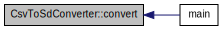
\includegraphics[width=294pt]{classCsvToSdConverter_a226c1dfaf88433cc9edf6570798231ec_icgraph}
\end{center}
\end{figure}


\hypertarget{classCsvToSdConverter_a83da8c064200da09a028d457a53263c5}{\index{Csv\-To\-Sd\-Converter@{Csv\-To\-Sd\-Converter}!get\-Text\-Block@{get\-Text\-Block}}
\index{get\-Text\-Block@{get\-Text\-Block}!CsvToSdConverter@{Csv\-To\-Sd\-Converter}}
\subsubsection[{get\-Text\-Block}]{\setlength{\rightskip}{0pt plus 5cm}string Csv\-To\-Sd\-Converter\-::get\-Text\-Block (
\begin{DoxyParamCaption}
\item[{string}]{data, }
\item[{int}]{n}
\end{DoxyParamCaption}
)\hspace{0.3cm}{\ttfamily [inline]}, {\ttfamily [protected]}}}\label{classCsvToSdConverter_a83da8c064200da09a028d457a53263c5}


Gibt den n-\/ten durch Leerzeichen abgetrennten Block aus einem String zurück. 


\begin{DoxyParams}{Parameter}
{\em data} & Der Ausgansstring. \\
\hline
{\em n} & Index des zu findenden Blocks. \\
\hline
\end{DoxyParams}
\begin{DoxyReturn}{Rückgabe}
Der n-\/te durch Leerzeichen getrennte Teilstring. \char`\"{}\char`\"{} Bei ungültigem Index. 
\end{DoxyReturn}


Definiert in Zeile 86 der Datei main.\-cpp.

\hypertarget{classCsvToSdConverter_adae10f022f4f05195c2a4b0a620d4645}{\index{Csv\-To\-Sd\-Converter@{Csv\-To\-Sd\-Converter}!parse\-Arguments@{parse\-Arguments}}
\index{parse\-Arguments@{parse\-Arguments}!CsvToSdConverter@{Csv\-To\-Sd\-Converter}}
\subsubsection[{parse\-Arguments}]{\setlength{\rightskip}{0pt plus 5cm}bool Csv\-To\-Sd\-Converter\-::parse\-Arguments (
\begin{DoxyParamCaption}
\item[{int}]{argc, }
\item[{char $\ast$}]{argv\mbox{[}$\,$\mbox{]}, }
\item[{string \&}]{sdef\-\_\-file, }
\item[{string \&}]{input\-\_\-file, }
\item[{string \&}]{output\-\_\-file}
\end{DoxyParamCaption}
)\hspace{0.3cm}{\ttfamily [inline]}, {\ttfamily [protected]}}}\label{classCsvToSdConverter_adae10f022f4f05195c2a4b0a620d4645}


Wertet die Programmargumente aus. 


\begin{DoxyParams}{Parameter}
{\em argc} & Anzahl der Programmargumente. \\
\hline
{\em argv} & Die Programmargumente. \\
\hline
{\em sdef\-\_\-file} & Ausgabe für den Pfad zur Sensordefinitionsdatei. \\
\hline
{\em input\-\_\-file} & Ausgabe für den Pfad zur Eingabedatei. \\
\hline
{\em output\-\_\-file} & Ausgabe für den Pfad zur Ausgabedatei. \\
\hline
\end{DoxyParams}
\begin{DoxyReturn}{Rückgabe}
Soll das Programm weiter ablaufen? 
\end{DoxyReturn}


Definiert in Zeile 345 der Datei main.\-cpp.

\hypertarget{classCsvToSdConverter_a4be5732a05287e3506925049ee990e1e}{\index{Csv\-To\-Sd\-Converter@{Csv\-To\-Sd\-Converter}!parse\-Line@{parse\-Line}}
\index{parse\-Line@{parse\-Line}!CsvToSdConverter@{Csv\-To\-Sd\-Converter}}
\subsubsection[{parse\-Line}]{\setlength{\rightskip}{0pt plus 5cm}void Csv\-To\-Sd\-Converter\-::parse\-Line (
\begin{DoxyParamCaption}
\item[{string}]{line, }
\item[{{\bf vector}$<$ string $>$ \&}]{out, }
\item[{{\bf vector}$<$ string $>$ $\ast$}]{timestamps, }
\item[{{\bf vector}$<$ string $>$ $\ast$}]{names, }
\item[{{\bf vector}$<$ int $>$ $\ast$}]{valid\-\_\-cols}
\end{DoxyParamCaption}
)\hspace{0.3cm}{\ttfamily [inline]}, {\ttfamily [protected]}}}\label{classCsvToSdConverter_a4be5732a05287e3506925049ee990e1e}


Sammelt Daten aus einer Textzeile (string). 


\begin{DoxyParams}{Parameter}
{\em line} & Die zu untersuchende Textzeile. \\
\hline
{\em out} & Ausgabevariable für die Sensordaten der Zeile. Alle Spalten nach opts.\-start\-\_\-col werden als Sensordatenspalten betrachtet. \\
\hline
{\em timestamps} & Wenn nicht N\-U\-L\-L, Ausgabevariable für den Zeitstempel der Zeile (opts.\-timecol). Der Zeitstempel wird an die übergebene Liste angehängt. \\
\hline
{\em names} & Wenn nicht N\-U\-L\-L, Ausgabevariable für den Namen der Zeile (opts.\-namecol). Der Name wird an die übergebene Liste angehängt. \\
\hline
{\em valid\-\_\-cols} & Wenn nicht N\-U\-L\-L, werden nur die Sensordaten-\/\-Spalten mit den Indices dieser Liste ausgewertet. \\
\hline
\end{DoxyParams}


Definiert in Zeile 126 der Datei main.\-cpp.

\hypertarget{classCsvToSdConverter_a6cfc076fd11f10d70767750a6aaf1f7c}{\index{Csv\-To\-Sd\-Converter@{Csv\-To\-Sd\-Converter}!read\-Configuration@{read\-Configuration}}
\index{read\-Configuration@{read\-Configuration}!CsvToSdConverter@{Csv\-To\-Sd\-Converter}}
\subsubsection[{read\-Configuration}]{\setlength{\rightskip}{0pt plus 5cm}bool Csv\-To\-Sd\-Converter\-::read\-Configuration (
\begin{DoxyParamCaption}
\item[{string}]{binary\-\_\-path}
\end{DoxyParamCaption}
)\hspace{0.3cm}{\ttfamily [inline]}, {\ttfamily [protected]}}}\label{classCsvToSdConverter_a6cfc076fd11f10d70767750a6aaf1f7c}


Liest und setzt die Programmkonfiguration aus der Konfigurationsdatei. 


\begin{DoxyParams}{Parameter}
{\em binary\-\_\-path} & Pfad zur Binärdatei. \\
\hline
\end{DoxyParams}
\begin{DoxyReturn}{Rückgabe}
War das Einlesen erfolgreich? 
\end{DoxyReturn}


Definiert in Zeile 208 der Datei main.\-cpp.



Hier ist ein Graph, der zeigt, was diese Funktion aufruft\-:\nopagebreak
\begin{figure}[H]
\begin{center}
\leavevmode
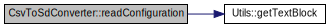
\includegraphics[width=350pt]{classCsvToSdConverter_a6cfc076fd11f10d70767750a6aaf1f7c_cgraph}
\end{center}
\end{figure}


\hypertarget{classCsvToSdConverter_ae6a8febba248592df4a0d0588018b67c}{\index{Csv\-To\-Sd\-Converter@{Csv\-To\-Sd\-Converter}!read\-Input\-File@{read\-Input\-File}}
\index{read\-Input\-File@{read\-Input\-File}!CsvToSdConverter@{Csv\-To\-Sd\-Converter}}
\subsubsection[{read\-Input\-File}]{\setlength{\rightskip}{0pt plus 5cm}bool Csv\-To\-Sd\-Converter\-::read\-Input\-File (
\begin{DoxyParamCaption}
\item[{string}]{path, }
\item[{{\bf vector}$<$ string $>$ \&}]{sensor\-\_\-names, }
\item[{{\bf vector}$<$ {\bf vector}$<$ string $>$ $>$ \&}]{values, }
\item[{{\bf vector}$<$ string $>$ \&}]{timestamps, }
\item[{{\bf vector}$<$ string $>$ \&}]{names}
\end{DoxyParamCaption}
)\hspace{0.3cm}{\ttfamily [inline]}, {\ttfamily [protected]}}}\label{classCsvToSdConverter_ae6a8febba248592df4a0d0588018b67c}


Liest die Daten aus der Eingabedatei. 


\begin{DoxyParams}{Parameter}
{\em path} & Der Pfad zur Eingabedatei. \\
\hline
{\em sensor\-\_\-names} & Liste der Namen der verwendeten Sensoren. \\
\hline
{\em values} & Liste für die extrahierten Sensorwerte. \\
\hline
{\em timestamps} & Liste für die Zeitstempel der Messwerte. \\
\hline
{\em names} & Liste für die Namen der Datensätze. \\
\hline
\end{DoxyParams}
\begin{DoxyReturn}{Rückgabe}
War das Einlesen erfolgreich? 
\end{DoxyReturn}


Definiert in Zeile 453 der Datei main.\-cpp.

\hypertarget{classCsvToSdConverter_aec2430ade6f76783c958d0b8466444c4}{\index{Csv\-To\-Sd\-Converter@{Csv\-To\-Sd\-Converter}!read\-Sensor\-Definitions@{read\-Sensor\-Definitions}}
\index{read\-Sensor\-Definitions@{read\-Sensor\-Definitions}!CsvToSdConverter@{Csv\-To\-Sd\-Converter}}
\subsubsection[{read\-Sensor\-Definitions}]{\setlength{\rightskip}{0pt plus 5cm}bool Csv\-To\-Sd\-Converter\-::read\-Sensor\-Definitions (
\begin{DoxyParamCaption}
\item[{string}]{path, }
\item[{{\bf vector}$<$ string $>$ $\ast$}]{sensor\-\_\-names, }
\item[{{\bf vector}$<$ string $>$ $\ast$}]{sensor\-\_\-data}
\end{DoxyParamCaption}
)\hspace{0.3cm}{\ttfamily [inline]}, {\ttfamily [protected]}}}\label{classCsvToSdConverter_aec2430ade6f76783c958d0b8466444c4}


Liest die Daten aus der Sensordefinitionsdatei. 


\begin{DoxyParams}{Parameter}
{\em path} & Pfad zur Binärdatei. \\
\hline
{\em sensor\-\_\-names} & Liste für die Namen der Sensoren. \\
\hline
{\em sensor\-\_\-data} & Liste für die Daten der Sensorden (Koordinaten). \\
\hline
\end{DoxyParams}
\begin{DoxyReturn}{Rückgabe}
War das Einlesen erfolgreich? 
\end{DoxyReturn}


Definiert in Zeile 264 der Datei main.\-cpp.

\hypertarget{classCsvToSdConverter_a16d31068591e8c70604267e34c0f0cb2}{\index{Csv\-To\-Sd\-Converter@{Csv\-To\-Sd\-Converter}!replace\-All@{replace\-All}}
\index{replace\-All@{replace\-All}!CsvToSdConverter@{Csv\-To\-Sd\-Converter}}
\subsubsection[{replace\-All}]{\setlength{\rightskip}{0pt plus 5cm}void Csv\-To\-Sd\-Converter\-::replace\-All (
\begin{DoxyParamCaption}
\item[{string \&}]{str, }
\item[{const string}]{from, }
\item[{const string}]{to}
\end{DoxyParamCaption}
)\hspace{0.3cm}{\ttfamily [inline]}, {\ttfamily [protected]}}}\label{classCsvToSdConverter_a16d31068591e8c70604267e34c0f0cb2}


Ersetzt in einem String alle Vorkommen eines Teilstrings durch einen Anderen. 


\begin{DoxyParams}{Parameter}
{\em str} & Der zu durchsuchende String. \\
\hline
{\em from} & Der zu ersetzende Teilstring. \\
\hline
{\em to} & Der Teilstring, durch den ersetzt werden soll. \\
\hline
\end{DoxyParams}


Definiert in Zeile 186 der Datei main.\-cpp.

\hypertarget{classCsvToSdConverter_a5a1749027e2c4dbe00feecc55b823226}{\index{Csv\-To\-Sd\-Converter@{Csv\-To\-Sd\-Converter}!write\-Output\-File@{write\-Output\-File}}
\index{write\-Output\-File@{write\-Output\-File}!CsvToSdConverter@{Csv\-To\-Sd\-Converter}}
\subsubsection[{write\-Output\-File}]{\setlength{\rightskip}{0pt plus 5cm}bool Csv\-To\-Sd\-Converter\-::write\-Output\-File (
\begin{DoxyParamCaption}
\item[{string}]{path, }
\item[{{\bf vector}$<$ string $>$ \&}]{sensor\-\_\-names, }
\item[{{\bf vector}$<$ string $>$ \&}]{sensor\-\_\-data, }
\item[{{\bf vector}$<$ {\bf vector}$<$ string $>$ $>$ \&}]{values, }
\item[{{\bf vector}$<$ string $>$ \&}]{timestamps, }
\item[{{\bf vector}$<$ string $>$ \&}]{names}
\end{DoxyParamCaption}
)\hspace{0.3cm}{\ttfamily [inline]}, {\ttfamily [protected]}}}\label{classCsvToSdConverter_a5a1749027e2c4dbe00feecc55b823226}


Schreibt die Ausgabedatei. 


\begin{DoxyParams}{Parameter}
{\em path} & Der Pfad zur Ausgabedatei. \\
\hline
{\em sensor\-\_\-names} & Liste der Namen der verwendeten Sensoren. \\
\hline
{\em sensor\-\_\-data} & Liste der Koordinaten der verwendeten Sensoren. \\
\hline
{\em values} & Liste für die extrahierten Sensorwerte. \\
\hline
{\em timestamps} & Liste für die Zeitstempel der Messwerte. \\
\hline
{\em names} & Liste für die Namen der Datensätze. \\
\hline
\end{DoxyParams}
\begin{DoxyReturn}{Rückgabe}
War das Schreiben erfolgreich? 
\end{DoxyReturn}


Definiert in Zeile 571 der Datei main.\-cpp.



\subsection{Dokumentation der Datenelemente}
\hypertarget{classCsvToSdConverter_a185377b44506f75748a4d56bc372ee50}{\index{Csv\-To\-Sd\-Converter@{Csv\-To\-Sd\-Converter}!configpaths@{configpaths}}
\index{configpaths@{configpaths}!CsvToSdConverter@{Csv\-To\-Sd\-Converter}}
\subsubsection[{configpaths}]{\setlength{\rightskip}{0pt plus 5cm}string Csv\-To\-Sd\-Converter\-::configpaths\mbox{[}{\bf N\-U\-M\-B\-E\-R\-O\-F\-P\-A\-T\-H\-S}\mbox{]}\hspace{0.3cm}{\ttfamily [protected]}}}\label{classCsvToSdConverter_a185377b44506f75748a4d56bc372ee50}
{\bfseries Initialisierung\-:}
\begin{DoxyCode}
\{
            \textcolor{stringliteral}{"/usr/local/share/simpleanalyzer/csvtosd.conf"},
            \textcolor{stringliteral}{"/usr/share/simpleanalyzer/csvtosd.conf"} \}
\end{DoxyCode}


Suchpfade für die Konfigurationsdatei. 

Das Verzeichnis der ausführbaren Datei wird immer geprüft. 

Definiert in Zeile 30 der Datei main.\-cpp.

\hypertarget{classCsvToSdConverter_ad2278682506407d3172e8fca834891fe}{\index{Csv\-To\-Sd\-Converter@{Csv\-To\-Sd\-Converter}!N\-U\-M\-B\-E\-R\-O\-F\-P\-A\-T\-H\-S@{N\-U\-M\-B\-E\-R\-O\-F\-P\-A\-T\-H\-S}}
\index{N\-U\-M\-B\-E\-R\-O\-F\-P\-A\-T\-H\-S@{N\-U\-M\-B\-E\-R\-O\-F\-P\-A\-T\-H\-S}!CsvToSdConverter@{Csv\-To\-Sd\-Converter}}
\subsubsection[{N\-U\-M\-B\-E\-R\-O\-F\-P\-A\-T\-H\-S}]{\setlength{\rightskip}{0pt plus 5cm}const int Csv\-To\-Sd\-Converter\-::\-N\-U\-M\-B\-E\-R\-O\-F\-P\-A\-T\-H\-S = 2\hspace{0.3cm}{\ttfamily [static]}, {\ttfamily [protected]}}}\label{classCsvToSdConverter_ad2278682506407d3172e8fca834891fe}


Anzahl der Suchpfade für die Konfigurationsdatei. 



Definiert in Zeile 24 der Datei main.\-cpp.

\hypertarget{classCsvToSdConverter_aed83889861a110c9913adb5b9f4d9eb3}{\index{Csv\-To\-Sd\-Converter@{Csv\-To\-Sd\-Converter}!opts@{opts}}
\index{opts@{opts}!CsvToSdConverter@{Csv\-To\-Sd\-Converter}}
\subsubsection[{opts}]{\setlength{\rightskip}{0pt plus 5cm}struct {\bf Csv\-To\-Sd\-Converter\-::\-Options}  Csv\-To\-Sd\-Converter\-::opts\hspace{0.3cm}{\ttfamily [protected]}}}\label{classCsvToSdConverter_aed83889861a110c9913adb5b9f4d9eb3}


Hält die verwendeten Programmeinstellungen. 



Die Dokumentation für diese Klasse wurde erzeugt aufgrund der Datei\-:\begin{DoxyCompactItemize}
\item 
/daten/\-Projekte/eclipse\-\_\-workspace/csvtosd/\hyperlink{csvtosd_2main_8cpp}{main.\-cpp}\end{DoxyCompactItemize}

\hypertarget{structUtils_1_1CutRender__info}{\section{Utils\-:\-:Cut\-Render\-\_\-info Strukturreferenz}
\label{structUtils_1_1CutRender__info}\index{Utils\-::\-Cut\-Render\-\_\-info@{Utils\-::\-Cut\-Render\-\_\-info}}
}


Daten zur Darstellung einer 2\-D-\/\-Temperaturverteilungs-\/\-Ebene.  




{\ttfamily \#include $<$utils.\-h$>$}



Zusammengehörigkeiten von Utils\-:\-:Cut\-Render\-\_\-info\-:\nopagebreak
\begin{figure}[H]
\begin{center}
\leavevmode
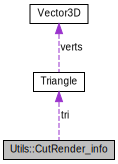
\includegraphics[width=190pt]{structUtils_1_1CutRender__info__coll__graph}
\end{center}
\end{figure}
\subsection*{Öffentliche Attribute}
\begin{DoxyCompactItemize}
\item 
\hyperlink{classTriangle}{Triangle} $\ast$ \hyperlink{structUtils_1_1CutRender__info_a2998343c733073b317fdd04bd341ce1f}{tri}
\begin{DoxyCompactList}\small\item\em Das die Ebene beschreibende Dreieck. \end{DoxyCompactList}\item 
float \hyperlink{structUtils_1_1CutRender__info_aca49d9537a774906b88f3fd7059d2dcb}{mmperpixel}
\begin{DoxyCompactList}\small\item\em Maßstab der Darstellung der Temperaturverteilung in $\frac{mm}{Pixel}$. \end{DoxyCompactList}\item 
int \hyperlink{structUtils_1_1CutRender__info_ac7a1e2c64129630affaf208808a190eb}{img\-\_\-width}
\begin{DoxyCompactList}\small\item\em Breite der Darstellung der Temperaturverteilung. \end{DoxyCompactList}\item 
int \hyperlink{structUtils_1_1CutRender__info_abac1c3e4edb7183017ecfa7b69c40d25}{img\-\_\-height}
\begin{DoxyCompactList}\small\item\em Höhe der Darstellung der Temperaturverteilung. \end{DoxyCompactList}\item 
\hyperlink{namespaceUtils_ad369b0127cabda0d6871ce1ae7e6c862}{P\-I\-M\-\_\-algorithm} \hyperlink{structUtils_1_1CutRender__info_af2ee1118ac14a73a2a350a05102013ab}{in\-\_\-volume\-\_\-algorithm}
\begin{DoxyCompactList}\small\item\em Der zu verwendende Punkt-\/in-\/\-Volumen-\/\-Testalgorithmus. \end{DoxyCompactList}\end{DoxyCompactItemize}


\subsection{Ausführliche Beschreibung}
Daten zur Darstellung einer 2\-D-\/\-Temperaturverteilungs-\/\-Ebene. 

Definiert in Zeile 78 der Datei utils.\-h.



\subsection{Dokumentation der Datenelemente}
\hypertarget{structUtils_1_1CutRender__info_abac1c3e4edb7183017ecfa7b69c40d25}{\index{Utils\-::\-Cut\-Render\-\_\-info@{Utils\-::\-Cut\-Render\-\_\-info}!img\-\_\-height@{img\-\_\-height}}
\index{img\-\_\-height@{img\-\_\-height}!Utils::CutRender_info@{Utils\-::\-Cut\-Render\-\_\-info}}
\subsubsection[{img\-\_\-height}]{\setlength{\rightskip}{0pt plus 5cm}int Utils\-::\-Cut\-Render\-\_\-info\-::img\-\_\-height}}\label{structUtils_1_1CutRender__info_abac1c3e4edb7183017ecfa7b69c40d25}


Höhe der Darstellung der Temperaturverteilung. 



Definiert in Zeile 82 der Datei utils.\-h.

\hypertarget{structUtils_1_1CutRender__info_ac7a1e2c64129630affaf208808a190eb}{\index{Utils\-::\-Cut\-Render\-\_\-info@{Utils\-::\-Cut\-Render\-\_\-info}!img\-\_\-width@{img\-\_\-width}}
\index{img\-\_\-width@{img\-\_\-width}!Utils::CutRender_info@{Utils\-::\-Cut\-Render\-\_\-info}}
\subsubsection[{img\-\_\-width}]{\setlength{\rightskip}{0pt plus 5cm}int Utils\-::\-Cut\-Render\-\_\-info\-::img\-\_\-width}}\label{structUtils_1_1CutRender__info_ac7a1e2c64129630affaf208808a190eb}


Breite der Darstellung der Temperaturverteilung. 



Definiert in Zeile 81 der Datei utils.\-h.

\hypertarget{structUtils_1_1CutRender__info_af2ee1118ac14a73a2a350a05102013ab}{\index{Utils\-::\-Cut\-Render\-\_\-info@{Utils\-::\-Cut\-Render\-\_\-info}!in\-\_\-volume\-\_\-algorithm@{in\-\_\-volume\-\_\-algorithm}}
\index{in\-\_\-volume\-\_\-algorithm@{in\-\_\-volume\-\_\-algorithm}!Utils::CutRender_info@{Utils\-::\-Cut\-Render\-\_\-info}}
\subsubsection[{in\-\_\-volume\-\_\-algorithm}]{\setlength{\rightskip}{0pt plus 5cm}{\bf P\-I\-M\-\_\-algorithm} Utils\-::\-Cut\-Render\-\_\-info\-::in\-\_\-volume\-\_\-algorithm}}\label{structUtils_1_1CutRender__info_af2ee1118ac14a73a2a350a05102013ab}


Der zu verwendende Punkt-\/in-\/\-Volumen-\/\-Testalgorithmus. 

Immer A\-L\-G\-O\-R\-I\-T\-H\-M\-\_\-\-T\-E\-T\-R\-A\-H\-E\-D\-R\-O\-N\-S. 

Definiert in Zeile 83 der Datei utils.\-h.

\hypertarget{structUtils_1_1CutRender__info_aca49d9537a774906b88f3fd7059d2dcb}{\index{Utils\-::\-Cut\-Render\-\_\-info@{Utils\-::\-Cut\-Render\-\_\-info}!mmperpixel@{mmperpixel}}
\index{mmperpixel@{mmperpixel}!Utils::CutRender_info@{Utils\-::\-Cut\-Render\-\_\-info}}
\subsubsection[{mmperpixel}]{\setlength{\rightskip}{0pt plus 5cm}float Utils\-::\-Cut\-Render\-\_\-info\-::mmperpixel}}\label{structUtils_1_1CutRender__info_aca49d9537a774906b88f3fd7059d2dcb}


Maßstab der Darstellung der Temperaturverteilung in $\frac{mm}{Pixel}$. 



Definiert in Zeile 80 der Datei utils.\-h.

\hypertarget{structUtils_1_1CutRender__info_a2998343c733073b317fdd04bd341ce1f}{\index{Utils\-::\-Cut\-Render\-\_\-info@{Utils\-::\-Cut\-Render\-\_\-info}!tri@{tri}}
\index{tri@{tri}!Utils::CutRender_info@{Utils\-::\-Cut\-Render\-\_\-info}}
\subsubsection[{tri}]{\setlength{\rightskip}{0pt plus 5cm}{\bf Triangle}$\ast$ Utils\-::\-Cut\-Render\-\_\-info\-::tri}}\label{structUtils_1_1CutRender__info_a2998343c733073b317fdd04bd341ce1f}


Das die Ebene beschreibende Dreieck. 

Der erste Punkt ist dabei das Zentrum der später ermittelten Temperaturverteilung. 

Definiert in Zeile 79 der Datei utils.\-h.



Die Dokumentation für diese Struktur wurde erzeugt aufgrund der Datei\-:\begin{DoxyCompactItemize}
\item 
/daten/\-Projekte/eclipse\-\_\-workspace/simpleanalyzer-\/gui/src/processing/\hyperlink{simpleanalyzer-gui_2src_2processing_2utils_8h}{utils.\-h}\end{DoxyCompactItemize}

\hypertarget{classExporter}{\section{Exporter Klassenreferenz}
\label{classExporter}\index{Exporter@{Exporter}}
}


Export der gewonnenen Daten.  




{\ttfamily \#include $<$Exporter.\-h$>$}

\subsection*{Öffentliche Methoden}
\begin{DoxyCompactItemize}
\item 
\hyperlink{classExporter_a2a977cb5ac8f637fcb570e73f650eca0}{Exporter} ()
\item 
\hyperlink{classObjectData_a20e8cd3cd0f8af3b571b9393aa9e6484}{Object\-Data\-::\-Object\-Data\-Status} \hyperlink{classExporter_a59d03f0a582498e15397230b70ad1e80}{Export\-Legacy\-V\-T\-K} (string filename, \hyperlink{classObjectData}{Object\-Data} $\ast$data)
\item 
\hyperlink{classObjectData_a20e8cd3cd0f8af3b571b9393aa9e6484}{Object\-Data\-::\-Object\-Data\-Status} \hyperlink{classExporter_ae2aa06b8c8c77e172801a1f77800ffd0}{Export\-Cut\-C\-S\-V} (string filename, float $\ast$values, \hyperlink{structUtils_1_1CutRender__info}{Cut\-Render\-\_\-info} $\ast$info)
\item 
virtual \hyperlink{classExporter_a44f24686958e01a543fd8b68b392658a}{$\sim$\-Exporter} ()
\end{DoxyCompactItemize}


\subsection{Ausführliche Beschreibung}
Export der gewonnenen Daten. 

Klasse zum Export der dreidimensionalen Temperaturverteilung als V\-T\-K-\/\-Datei und der zweidimensionalen Temperaturverteilung (Schnitt durch das Modell) als .csv-\/\-Datei. 

\subsection{Beschreibung der Konstruktoren und Destruktoren}
\hypertarget{classExporter_a2a977cb5ac8f637fcb570e73f650eca0}{\index{Exporter@{Exporter}!Exporter@{Exporter}}
\index{Exporter@{Exporter}!Exporter@{Exporter}}
\subsubsection[{Exporter}]{\setlength{\rightskip}{0pt plus 5cm}Exporter\-::\-Exporter (
\begin{DoxyParamCaption}
{}
\end{DoxyParamCaption}
)}}\label{classExporter_a2a977cb5ac8f637fcb570e73f650eca0}
Der Konstruktor. \hypertarget{classExporter_a44f24686958e01a543fd8b68b392658a}{\index{Exporter@{Exporter}!$\sim$\-Exporter@{$\sim$\-Exporter}}
\index{$\sim$\-Exporter@{$\sim$\-Exporter}!Exporter@{Exporter}}
\subsubsection[{$\sim$\-Exporter}]{\setlength{\rightskip}{0pt plus 5cm}Exporter\-::$\sim$\-Exporter (
\begin{DoxyParamCaption}
{}
\end{DoxyParamCaption}
)\hspace{0.3cm}{\ttfamily [virtual]}}}\label{classExporter_a44f24686958e01a543fd8b68b392658a}
Der Destruktor. 

\subsection{Dokumentation der Elementfunktionen}
\hypertarget{classExporter_ae2aa06b8c8c77e172801a1f77800ffd0}{\index{Exporter@{Exporter}!Export\-Cut\-C\-S\-V@{Export\-Cut\-C\-S\-V}}
\index{Export\-Cut\-C\-S\-V@{Export\-Cut\-C\-S\-V}!Exporter@{Exporter}}
\subsubsection[{Export\-Cut\-C\-S\-V}]{\setlength{\rightskip}{0pt plus 5cm}{\bf Object\-Data\-::\-Object\-Data\-Status} Exporter\-::\-Export\-Cut\-C\-S\-V (
\begin{DoxyParamCaption}
\item[{string}]{filename, }
\item[{float $\ast$}]{values, }
\item[{{\bf Cut\-Render\-\_\-info} $\ast$}]{info}
\end{DoxyParamCaption}
)}}\label{classExporter_ae2aa06b8c8c77e172801a1f77800ffd0}
Exportiert die zweidimensionale Temperaturverteilung (Schnitt durch das Modell) als csv-\/\-Datei. \begin{DoxyReturn}{Rückgabe}
Der Fehlercode. 
\end{DoxyReturn}
\hypertarget{classExporter_a59d03f0a582498e15397230b70ad1e80}{\index{Exporter@{Exporter}!Export\-Legacy\-V\-T\-K@{Export\-Legacy\-V\-T\-K}}
\index{Export\-Legacy\-V\-T\-K@{Export\-Legacy\-V\-T\-K}!Exporter@{Exporter}}
\subsubsection[{Export\-Legacy\-V\-T\-K}]{\setlength{\rightskip}{0pt plus 5cm}{\bf Object\-Data\-::\-Object\-Data\-Status} Exporter\-::\-Export\-Legacy\-V\-T\-K (
\begin{DoxyParamCaption}
\item[{string}]{filename, }
\item[{{\bf Object\-Data} $\ast$}]{data}
\end{DoxyParamCaption}
)}}\label{classExporter_a59d03f0a582498e15397230b70ad1e80}
Exportiert die aktuell berechnete dreidimensionale Temperaturverteilung und das Modell als V\-T\-K-\/\-Datei. \begin{DoxyReturn}{Rückgabe}
Der Fehlercode. 
\end{DoxyReturn}


Die Dokumentation für diese Klasse wurde erzeugt aufgrund der Dateien\-:\begin{DoxyCompactItemize}
\item 
simpleanalyzer-\/gui/src/file\-I\-O/Exporter.\-h\item 
simpleanalyzer-\/gui/src/file\-I\-O/Exporter.\-cpp\end{DoxyCompactItemize}

\hypertarget{classGUIAnalyzeOutputWindow}{\section{G\-U\-I\-Analyze\-Output\-Window Klassenreferenz}
\label{classGUIAnalyzeOutputWindow}\index{G\-U\-I\-Analyze\-Output\-Window@{G\-U\-I\-Analyze\-Output\-Window}}
}


Übersichtsfenster über die Analysedaten.  




{\ttfamily \#include $<$G\-U\-I\-Analyze\-Output\-Window.\-h$>$}



Klassendiagramm für G\-U\-I\-Analyze\-Output\-Window\-:
\nopagebreak
\begin{figure}[H]
\begin{center}
\leavevmode
\includegraphics[width=214pt]{classGUIAnalyzeOutputWindow__inherit__graph}
\end{center}
\end{figure}


Zusammengehörigkeiten von G\-U\-I\-Analyze\-Output\-Window\-:
\nopagebreak
\begin{figure}[H]
\begin{center}
\leavevmode
\includegraphics[width=214pt]{classGUIAnalyzeOutputWindow__coll__graph}
\end{center}
\end{figure}
\subsection*{Öffentliche Methoden}
\begin{DoxyCompactItemize}
\item 
\hyperlink{classGUIAnalyzeOutputWindow_af9407245a6b2a0478579c4d592a31e63}{G\-U\-I\-Analyze\-Output\-Window} (wx\-Window $\ast$parent, const wx\-Char $\ast$title, int xpos, int ypos, int width, int height)
\begin{DoxyCompactList}\small\item\em Der Konstruktor. \end{DoxyCompactList}\item 
void \hyperlink{classGUIAnalyzeOutputWindow_a9ea5a7cf46d6189f368315903508cecc}{Update} ()
\begin{DoxyCompactList}\small\item\em Methode zum aktualisieren des Fensters, alle Objekte werden erneut analysiert und die aktualisierten Ergebnisse angezeigt. \end{DoxyCompactList}\item 
virtual \hyperlink{classGUIAnalyzeOutputWindow_a8c5f2447557358ea724b68a89f363e37}{$\sim$\-G\-U\-I\-Analyze\-Output\-Window} ()
\begin{DoxyCompactList}\small\item\em Der Destruktor. \end{DoxyCompactList}\end{DoxyCompactItemize}
\subsection*{Private Methoden}
\begin{DoxyCompactItemize}
\item 
void \hyperlink{classGUIAnalyzeOutputWindow_ab574494affda3239c7a7a28c6dc347de}{On\-Key\-Press} (wx\-Key\-Event \&event)
\begin{DoxyCompactList}\small\item\em Event-\/\-Tabellendeklaration für wx\-Widgets. \end{DoxyCompactList}\item 
void \hyperlink{classGUIAnalyzeOutputWindow_a1543bc16c0c5722fb961bea8d6462bb6}{Select\-All} ()
\begin{DoxyCompactList}\small\item\em Selektiert alle Zellen der Tabelle. \end{DoxyCompactList}\item 
void \hyperlink{classGUIAnalyzeOutputWindow_a9a25abd50d7d0bd163143924594385f4}{To\-Clipboard} ()
\begin{DoxyCompactList}\small\item\em Kopiert die Inhalte der Tabelle in die Zwischenablage. \end{DoxyCompactList}\end{DoxyCompactItemize}
\subsection*{Private Attribute}
\begin{DoxyCompactItemize}
\item 
wx\-Grid $\ast$ \hyperlink{classGUIAnalyzeOutputWindow_afa1bc15fd767bfb9922e880403fb4305}{table}
\begin{DoxyCompactList}\small\item\em Die Tabellenkomponente. \end{DoxyCompactList}\end{DoxyCompactItemize}


\subsection{Ausführliche Beschreibung}
Übersichtsfenster über die Analysedaten. 

Dieses Fenster zeigt eine Tabelle mit den zur Analyse markierten Zeitpunkten für alle Objekte und deren\-Datensätze und Materialen. Nicht-\/zeitabhängige Sensordaten werden immer angezeigt. 

Definiert in Zeile 22 der Datei G\-U\-I\-Analyze\-Output\-Window.\-h.



\subsection{Beschreibung der Konstruktoren und Destruktoren}
\hypertarget{classGUIAnalyzeOutputWindow_af9407245a6b2a0478579c4d592a31e63}{\index{G\-U\-I\-Analyze\-Output\-Window@{G\-U\-I\-Analyze\-Output\-Window}!G\-U\-I\-Analyze\-Output\-Window@{G\-U\-I\-Analyze\-Output\-Window}}
\index{G\-U\-I\-Analyze\-Output\-Window@{G\-U\-I\-Analyze\-Output\-Window}!GUIAnalyzeOutputWindow@{G\-U\-I\-Analyze\-Output\-Window}}
\subsubsection[{G\-U\-I\-Analyze\-Output\-Window}]{\setlength{\rightskip}{0pt plus 5cm}G\-U\-I\-Analyze\-Output\-Window\-::\-G\-U\-I\-Analyze\-Output\-Window (
\begin{DoxyParamCaption}
\item[{wx\-Window $\ast$}]{parent, }
\item[{const wx\-Char $\ast$}]{title, }
\item[{int}]{xpos, }
\item[{int}]{ypos, }
\item[{int}]{width, }
\item[{int}]{height}
\end{DoxyParamCaption}
)}}\label{classGUIAnalyzeOutputWindow_af9407245a6b2a0478579c4d592a31e63}


Der Konstruktor. 



Definiert in Zeile 23 der Datei G\-U\-I\-Analyze\-Output\-Window.\-cpp.

\hypertarget{classGUIAnalyzeOutputWindow_a8c5f2447557358ea724b68a89f363e37}{\index{G\-U\-I\-Analyze\-Output\-Window@{G\-U\-I\-Analyze\-Output\-Window}!$\sim$\-G\-U\-I\-Analyze\-Output\-Window@{$\sim$\-G\-U\-I\-Analyze\-Output\-Window}}
\index{$\sim$\-G\-U\-I\-Analyze\-Output\-Window@{$\sim$\-G\-U\-I\-Analyze\-Output\-Window}!GUIAnalyzeOutputWindow@{G\-U\-I\-Analyze\-Output\-Window}}
\subsubsection[{$\sim$\-G\-U\-I\-Analyze\-Output\-Window}]{\setlength{\rightskip}{0pt plus 5cm}G\-U\-I\-Analyze\-Output\-Window\-::$\sim$\-G\-U\-I\-Analyze\-Output\-Window (
\begin{DoxyParamCaption}
{}
\end{DoxyParamCaption}
)\hspace{0.3cm}{\ttfamily [virtual]}}}\label{classGUIAnalyzeOutputWindow_a8c5f2447557358ea724b68a89f363e37}


Der Destruktor. 



Definiert in Zeile 210 der Datei G\-U\-I\-Analyze\-Output\-Window.\-cpp.



Hier ist ein Graph, der zeigt, was diese Funktion aufruft\-:\nopagebreak
\begin{figure}[H]
\begin{center}
\leavevmode
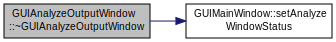
\includegraphics[width=350pt]{classGUIAnalyzeOutputWindow_a8c5f2447557358ea724b68a89f363e37_cgraph}
\end{center}
\end{figure}




\subsection{Dokumentation der Elementfunktionen}
\hypertarget{classGUIAnalyzeOutputWindow_ab574494affda3239c7a7a28c6dc347de}{\index{G\-U\-I\-Analyze\-Output\-Window@{G\-U\-I\-Analyze\-Output\-Window}!On\-Key\-Press@{On\-Key\-Press}}
\index{On\-Key\-Press@{On\-Key\-Press}!GUIAnalyzeOutputWindow@{G\-U\-I\-Analyze\-Output\-Window}}
\subsubsection[{On\-Key\-Press}]{\setlength{\rightskip}{0pt plus 5cm}void G\-U\-I\-Analyze\-Output\-Window\-::\-On\-Key\-Press (
\begin{DoxyParamCaption}
\item[{wx\-Key\-Event \&}]{event}
\end{DoxyParamCaption}
)\hspace{0.3cm}{\ttfamily [private]}}}\label{classGUIAnalyzeOutputWindow_ab574494affda3239c7a7a28c6dc347de}


Event-\/\-Tabellendeklaration für wx\-Widgets. 

Behandelt das Drücken von Strg+\-C und Strg+\-A. 

Definiert in Zeile 197 der Datei G\-U\-I\-Analyze\-Output\-Window.\-cpp.

\hypertarget{classGUIAnalyzeOutputWindow_a1543bc16c0c5722fb961bea8d6462bb6}{\index{G\-U\-I\-Analyze\-Output\-Window@{G\-U\-I\-Analyze\-Output\-Window}!Select\-All@{Select\-All}}
\index{Select\-All@{Select\-All}!GUIAnalyzeOutputWindow@{G\-U\-I\-Analyze\-Output\-Window}}
\subsubsection[{Select\-All}]{\setlength{\rightskip}{0pt plus 5cm}void G\-U\-I\-Analyze\-Output\-Window\-::\-Select\-All (
\begin{DoxyParamCaption}
{}
\end{DoxyParamCaption}
)\hspace{0.3cm}{\ttfamily [private]}}}\label{classGUIAnalyzeOutputWindow_a1543bc16c0c5722fb961bea8d6462bb6}


Selektiert alle Zellen der Tabelle. 



Definiert in Zeile 189 der Datei G\-U\-I\-Analyze\-Output\-Window.\-cpp.

\hypertarget{classGUIAnalyzeOutputWindow_a9a25abd50d7d0bd163143924594385f4}{\index{G\-U\-I\-Analyze\-Output\-Window@{G\-U\-I\-Analyze\-Output\-Window}!To\-Clipboard@{To\-Clipboard}}
\index{To\-Clipboard@{To\-Clipboard}!GUIAnalyzeOutputWindow@{G\-U\-I\-Analyze\-Output\-Window}}
\subsubsection[{To\-Clipboard}]{\setlength{\rightskip}{0pt plus 5cm}void G\-U\-I\-Analyze\-Output\-Window\-::\-To\-Clipboard (
\begin{DoxyParamCaption}
{}
\end{DoxyParamCaption}
)\hspace{0.3cm}{\ttfamily [private]}}}\label{classGUIAnalyzeOutputWindow_a9a25abd50d7d0bd163143924594385f4}


Kopiert die Inhalte der Tabelle in die Zwischenablage. 

Basierend auf \href{http://forums.wxwidgets.org/viewtopic.php?f=20&t=2200#p148731}{\tt http\-://forums.\-wxwidgets.\-org/viewtopic.\-php?f=20\&t=2200\#p148731}. 

Definiert in Zeile 151 der Datei G\-U\-I\-Analyze\-Output\-Window.\-cpp.

\hypertarget{classGUIAnalyzeOutputWindow_a9ea5a7cf46d6189f368315903508cecc}{\index{G\-U\-I\-Analyze\-Output\-Window@{G\-U\-I\-Analyze\-Output\-Window}!Update@{Update}}
\index{Update@{Update}!GUIAnalyzeOutputWindow@{G\-U\-I\-Analyze\-Output\-Window}}
\subsubsection[{Update}]{\setlength{\rightskip}{0pt plus 5cm}void G\-U\-I\-Analyze\-Output\-Window\-::\-Update (
\begin{DoxyParamCaption}
{}
\end{DoxyParamCaption}
)}}\label{classGUIAnalyzeOutputWindow_a9ea5a7cf46d6189f368315903508cecc}


Methode zum aktualisieren des Fensters, alle Objekte werden erneut analysiert und die aktualisierten Ergebnisse angezeigt. 



Definiert in Zeile 37 der Datei G\-U\-I\-Analyze\-Output\-Window.\-cpp.



Hier ist ein Graph, der zeigt, was diese Funktion aufruft\-:\nopagebreak
\begin{figure}[H]
\begin{center}
\leavevmode
\includegraphics[width=350pt]{classGUIAnalyzeOutputWindow_a9ea5a7cf46d6189f368315903508cecc_cgraph}
\end{center}
\end{figure}




\subsection{Dokumentation der Datenelemente}
\hypertarget{classGUIAnalyzeOutputWindow_afa1bc15fd767bfb9922e880403fb4305}{\index{G\-U\-I\-Analyze\-Output\-Window@{G\-U\-I\-Analyze\-Output\-Window}!table@{table}}
\index{table@{table}!GUIAnalyzeOutputWindow@{G\-U\-I\-Analyze\-Output\-Window}}
\subsubsection[{table}]{\setlength{\rightskip}{0pt plus 5cm}wx\-Grid$\ast$ G\-U\-I\-Analyze\-Output\-Window\-::table\hspace{0.3cm}{\ttfamily [private]}}}\label{classGUIAnalyzeOutputWindow_afa1bc15fd767bfb9922e880403fb4305}


Die Tabellenkomponente. 



Definiert in Zeile 65 der Datei G\-U\-I\-Analyze\-Output\-Window.\-h.



Die Dokumentation für diese Klasse wurde erzeugt aufgrund der Dateien\-:\begin{DoxyCompactItemize}
\item 
/daten/\-Projekte/eclipse\-\_\-workspace/simpleanalyzer-\/gui/src/\-G\-U\-I/\hyperlink{GUIAnalyzeOutputWindow_8h}{G\-U\-I\-Analyze\-Output\-Window.\-h}\item 
/daten/\-Projekte/eclipse\-\_\-workspace/simpleanalyzer-\/gui/src/\-G\-U\-I/\hyperlink{GUIAnalyzeOutputWindow_8cpp}{G\-U\-I\-Analyze\-Output\-Window.\-cpp}\end{DoxyCompactItemize}

\hypertarget{classGUIAnalyzePointWindow}{\section{G\-U\-I\-Analyze\-Point\-Window Klassenreferenz}
\label{classGUIAnalyzePointWindow}\index{G\-U\-I\-Analyze\-Point\-Window@{G\-U\-I\-Analyze\-Point\-Window}}
}


Analysefenster für einen Punkt.  




{\ttfamily \#include $<$G\-U\-I\-Analyze\-Point\-Window.\-h$>$}

Klassendiagramm für G\-U\-I\-Analyze\-Point\-Window\-:\begin{figure}[H]
\begin{center}
\leavevmode
\includegraphics[height=2.000000cm]{classGUIAnalyzePointWindow}
\end{center}
\end{figure}
\subsection*{Öffentliche Methoden}
\begin{DoxyCompactItemize}
\item 
\hyperlink{classGUIAnalyzePointWindow_abf699fcd4ffb8bec8b0565e6404b0af3}{G\-U\-I\-Analyze\-Point\-Window} (wx\-Window $\ast$parent, const wx\-Char $\ast$title, int xpos, int ypos, int width, int height)
\item 
virtual \hyperlink{classGUIAnalyzePointWindow_a9edaece1fef847902309af1f63eb168a}{$\sim$\-G\-U\-I\-Analyze\-Point\-Window} ()
\end{DoxyCompactItemize}
\subsection*{Private Methoden}
\begin{DoxyCompactItemize}
\item 
void \hyperlink{classGUIAnalyzePointWindow_aa84ea9958e8b41423f01316d01ba5151}{analyze\-Point} (wx\-Command\-Event \&event)
\end{DoxyCompactItemize}
\subsection*{Private Attribute}
\begin{DoxyCompactItemize}
\item 
wx\-Static\-Text $\ast$ \hyperlink{classGUIAnalyzePointWindow_ae3f474800a7f7d9e4a897bdf33510f01}{label}
\item 
wx\-Text\-Ctrl $\ast$ \hyperlink{classGUIAnalyzePointWindow_a4c3d50b2c5c38b8b757cdb1c04ea83b6}{xedit}
\item 
wx\-Text\-Ctrl $\ast$ \hyperlink{classGUIAnalyzePointWindow_ac4352df05ac2a001551801a90fc8bc42}{yedit}
\item 
wx\-Text\-Ctrl $\ast$ \hyperlink{classGUIAnalyzePointWindow_a173e639b35cc6c18a74fb746b8664c8c}{zedit}
\item 
wx\-Static\-Text $\ast$ \hyperlink{classGUIAnalyzePointWindow_a6a1b5c74ab4aca0f3ccea3ef83043b35}{interpolation\-Mode\-Label}
\item 
wx\-Combo\-Box $\ast$ \hyperlink{classGUIAnalyzePointWindow_a6b2da34e788e56e70789d2cfc9767357}{interpolation\-Mode\-List}
\item 
wx\-Button $\ast$ \hyperlink{classGUIAnalyzePointWindow_a2650076436d57254fa9dd0df3783593e}{calcbt}
\end{DoxyCompactItemize}


\subsection{Ausführliche Beschreibung}
Analysefenster für einen Punkt. 

\subsection{Beschreibung der Konstruktoren und Destruktoren}
\hypertarget{classGUIAnalyzePointWindow_abf699fcd4ffb8bec8b0565e6404b0af3}{\index{G\-U\-I\-Analyze\-Point\-Window@{G\-U\-I\-Analyze\-Point\-Window}!G\-U\-I\-Analyze\-Point\-Window@{G\-U\-I\-Analyze\-Point\-Window}}
\index{G\-U\-I\-Analyze\-Point\-Window@{G\-U\-I\-Analyze\-Point\-Window}!GUIAnalyzePointWindow@{G\-U\-I\-Analyze\-Point\-Window}}
\subsubsection[{G\-U\-I\-Analyze\-Point\-Window}]{\setlength{\rightskip}{0pt plus 5cm}G\-U\-I\-Analyze\-Point\-Window\-::\-G\-U\-I\-Analyze\-Point\-Window (
\begin{DoxyParamCaption}
\item[{wx\-Window $\ast$}]{parent, }
\item[{const wx\-Char $\ast$}]{title, }
\item[{int}]{xpos, }
\item[{int}]{ypos, }
\item[{int}]{width, }
\item[{int}]{height}
\end{DoxyParamCaption}
)}}\label{classGUIAnalyzePointWindow_abf699fcd4ffb8bec8b0565e6404b0af3}
Der Konstruktor. \hypertarget{classGUIAnalyzePointWindow_a9edaece1fef847902309af1f63eb168a}{\index{G\-U\-I\-Analyze\-Point\-Window@{G\-U\-I\-Analyze\-Point\-Window}!$\sim$\-G\-U\-I\-Analyze\-Point\-Window@{$\sim$\-G\-U\-I\-Analyze\-Point\-Window}}
\index{$\sim$\-G\-U\-I\-Analyze\-Point\-Window@{$\sim$\-G\-U\-I\-Analyze\-Point\-Window}!GUIAnalyzePointWindow@{G\-U\-I\-Analyze\-Point\-Window}}
\subsubsection[{$\sim$\-G\-U\-I\-Analyze\-Point\-Window}]{\setlength{\rightskip}{0pt plus 5cm}G\-U\-I\-Analyze\-Point\-Window\-::$\sim$\-G\-U\-I\-Analyze\-Point\-Window (
\begin{DoxyParamCaption}
{}
\end{DoxyParamCaption}
)\hspace{0.3cm}{\ttfamily [virtual]}}}\label{classGUIAnalyzePointWindow_a9edaece1fef847902309af1f63eb168a}
Der Destruktor. 

\subsection{Dokumentation der Elementfunktionen}
\hypertarget{classGUIAnalyzePointWindow_aa84ea9958e8b41423f01316d01ba5151}{\index{G\-U\-I\-Analyze\-Point\-Window@{G\-U\-I\-Analyze\-Point\-Window}!analyze\-Point@{analyze\-Point}}
\index{analyze\-Point@{analyze\-Point}!GUIAnalyzePointWindow@{G\-U\-I\-Analyze\-Point\-Window}}
\subsubsection[{analyze\-Point}]{\setlength{\rightskip}{0pt plus 5cm}void G\-U\-I\-Analyze\-Point\-Window\-::analyze\-Point (
\begin{DoxyParamCaption}
\item[{wx\-Command\-Event \&}]{event}
\end{DoxyParamCaption}
)\hspace{0.3cm}{\ttfamily [private]}}}\label{classGUIAnalyzePointWindow_aa84ea9958e8b41423f01316d01ba5151}
Event-\/\-Tabellendeklaration für wx\-Widgets. Ermittelt Temperatur und Art des Punktes (Interpoliert/\-Extrapoliert). Wird durch Event ausgelöst. 

\subsection{Dokumentation der Datenelemente}
\hypertarget{classGUIAnalyzePointWindow_a2650076436d57254fa9dd0df3783593e}{\index{G\-U\-I\-Analyze\-Point\-Window@{G\-U\-I\-Analyze\-Point\-Window}!calcbt@{calcbt}}
\index{calcbt@{calcbt}!GUIAnalyzePointWindow@{G\-U\-I\-Analyze\-Point\-Window}}
\subsubsection[{calcbt}]{\setlength{\rightskip}{0pt plus 5cm}wx\-Button$\ast$ G\-U\-I\-Analyze\-Point\-Window\-::calcbt\hspace{0.3cm}{\ttfamily [private]}}}\label{classGUIAnalyzePointWindow_a2650076436d57254fa9dd0df3783593e}
Button zum Auslösen der Analyseprozedur. \hypertarget{classGUIAnalyzePointWindow_a6a1b5c74ab4aca0f3ccea3ef83043b35}{\index{G\-U\-I\-Analyze\-Point\-Window@{G\-U\-I\-Analyze\-Point\-Window}!interpolation\-Mode\-Label@{interpolation\-Mode\-Label}}
\index{interpolation\-Mode\-Label@{interpolation\-Mode\-Label}!GUIAnalyzePointWindow@{G\-U\-I\-Analyze\-Point\-Window}}
\subsubsection[{interpolation\-Mode\-Label}]{\setlength{\rightskip}{0pt plus 5cm}wx\-Static\-Text$\ast$ G\-U\-I\-Analyze\-Point\-Window\-::interpolation\-Mode\-Label\hspace{0.3cm}{\ttfamily [private]}}}\label{classGUIAnalyzePointWindow_a6a1b5c74ab4aca0f3ccea3ef83043b35}
Beschriftung für den Interpolationsmodus. \hypertarget{classGUIAnalyzePointWindow_a6b2da34e788e56e70789d2cfc9767357}{\index{G\-U\-I\-Analyze\-Point\-Window@{G\-U\-I\-Analyze\-Point\-Window}!interpolation\-Mode\-List@{interpolation\-Mode\-List}}
\index{interpolation\-Mode\-List@{interpolation\-Mode\-List}!GUIAnalyzePointWindow@{G\-U\-I\-Analyze\-Point\-Window}}
\subsubsection[{interpolation\-Mode\-List}]{\setlength{\rightskip}{0pt plus 5cm}wx\-Combo\-Box$\ast$ G\-U\-I\-Analyze\-Point\-Window\-::interpolation\-Mode\-List\hspace{0.3cm}{\ttfamily [private]}}}\label{classGUIAnalyzePointWindow_a6b2da34e788e56e70789d2cfc9767357}
Dropdown-\/\-Menü für den Interpolationsmodus. \hypertarget{classGUIAnalyzePointWindow_ae3f474800a7f7d9e4a897bdf33510f01}{\index{G\-U\-I\-Analyze\-Point\-Window@{G\-U\-I\-Analyze\-Point\-Window}!label@{label}}
\index{label@{label}!GUIAnalyzePointWindow@{G\-U\-I\-Analyze\-Point\-Window}}
\subsubsection[{label}]{\setlength{\rightskip}{0pt plus 5cm}wx\-Static\-Text$\ast$ G\-U\-I\-Analyze\-Point\-Window\-::label\hspace{0.3cm}{\ttfamily [private]}}}\label{classGUIAnalyzePointWindow_ae3f474800a7f7d9e4a897bdf33510f01}
Beschriftung der Fensterkomponenten. \hypertarget{classGUIAnalyzePointWindow_a4c3d50b2c5c38b8b757cdb1c04ea83b6}{\index{G\-U\-I\-Analyze\-Point\-Window@{G\-U\-I\-Analyze\-Point\-Window}!xedit@{xedit}}
\index{xedit@{xedit}!GUIAnalyzePointWindow@{G\-U\-I\-Analyze\-Point\-Window}}
\subsubsection[{xedit}]{\setlength{\rightskip}{0pt plus 5cm}wx\-Text\-Ctrl$\ast$ G\-U\-I\-Analyze\-Point\-Window\-::xedit\hspace{0.3cm}{\ttfamily [private]}}}\label{classGUIAnalyzePointWindow_a4c3d50b2c5c38b8b757cdb1c04ea83b6}
Eingabefeld für die X-\/\-Koordinate. \hypertarget{classGUIAnalyzePointWindow_ac4352df05ac2a001551801a90fc8bc42}{\index{G\-U\-I\-Analyze\-Point\-Window@{G\-U\-I\-Analyze\-Point\-Window}!yedit@{yedit}}
\index{yedit@{yedit}!GUIAnalyzePointWindow@{G\-U\-I\-Analyze\-Point\-Window}}
\subsubsection[{yedit}]{\setlength{\rightskip}{0pt plus 5cm}wx\-Text\-Ctrl$\ast$ G\-U\-I\-Analyze\-Point\-Window\-::yedit\hspace{0.3cm}{\ttfamily [private]}}}\label{classGUIAnalyzePointWindow_ac4352df05ac2a001551801a90fc8bc42}
Eingabefeld für die Y-\/\-Koordinate. \hypertarget{classGUIAnalyzePointWindow_a173e639b35cc6c18a74fb746b8664c8c}{\index{G\-U\-I\-Analyze\-Point\-Window@{G\-U\-I\-Analyze\-Point\-Window}!zedit@{zedit}}
\index{zedit@{zedit}!GUIAnalyzePointWindow@{G\-U\-I\-Analyze\-Point\-Window}}
\subsubsection[{zedit}]{\setlength{\rightskip}{0pt plus 5cm}wx\-Text\-Ctrl$\ast$ G\-U\-I\-Analyze\-Point\-Window\-::zedit\hspace{0.3cm}{\ttfamily [private]}}}\label{classGUIAnalyzePointWindow_a173e639b35cc6c18a74fb746b8664c8c}
Eingabefeld für die Z-\/\-Koordinate. 

Die Dokumentation für diese Klasse wurde erzeugt aufgrund der Dateien\-:\begin{DoxyCompactItemize}
\item 
simpleanalyzer-\/gui/src/\-G\-U\-I/G\-U\-I\-Analyze\-Point\-Window.\-h\item 
simpleanalyzer-\/gui/src/\-G\-U\-I/G\-U\-I\-Analyze\-Point\-Window.\-cpp\end{DoxyCompactItemize}

\hypertarget{classGUIColorScalePanel}{\section{G\-U\-I\-Color\-Scale\-Panel Klassenreferenz}
\label{classGUIColorScalePanel}\index{G\-U\-I\-Color\-Scale\-Panel@{G\-U\-I\-Color\-Scale\-Panel}}
}


Farbige Temperaturskala für zweidimensionale Temperaturverteilung.  




{\ttfamily \#include $<$G\-U\-I\-Color\-Scale\-Panel.\-h$>$}

\subsection*{Öffentliche Typen}
\begin{DoxyCompactItemize}
\item 
enum {\bfseries Scale\-Mode} \{ {\bfseries S\-C\-M\-\_\-\-N\-O\-N\-E} = 0, 
{\bfseries S\-C\-M\-\_\-\-H\-O\-R\-I\-Z\-O\-N\-T\-A\-L}, 
{\bfseries S\-C\-M\-\_\-\-V\-E\-R\-T\-I\-C\-A\-L}
 \}
\end{DoxyCompactItemize}
\subsection*{Öffentliche Methoden}
\begin{DoxyCompactItemize}
\item 
\hyperlink{classGUIColorScalePanel_ad4ad453f831d149cc9fde46cba883431}{G\-U\-I\-Color\-Scale\-Panel} ()
\item 
void \hyperlink{classGUIColorScalePanel_a73f647d4f5eeb6b653777bb4c55696fa}{refresh} (int img\-\_\-width, int img\-\_\-height)
\item 
void \hyperlink{classGUIColorScalePanel_aaf6408cc09932a82afc7b2c233ec64c8}{paint\-To} (wx\-D\-C \&dc, float zoom, wx\-Point \&img\-\_\-coords)
\item 
void \hyperlink{classGUIColorScalePanel_a59e27a091ec86d4c3e649f432a10ec08}{handle\-Mouse} (wx\-Mouse\-Event \&event, wx\-Point \&img\-\_\-coords, wx\-Point \&img\-\_\-dim, float zoom)
\item 
void \hyperlink{classGUIColorScalePanel_aa7d5eb68ecd55e23b2e8969a21c32a22}{get\-Display\-Area} (wx\-Rect $\ast$rect, float zoom)
\item 
void \hyperlink{classGUIColorScalePanel_ac8faaae6f7016f0fecedfc350b65644b}{fit\-Bounds} (wx\-Point \&img\-\_\-dim, bool to\-\_\-scale)
\item 
bool \hyperlink{classGUIColorScalePanel_a4b17b0a63d3921ce09ffe5a99b6955a5}{mouse\-On\-Display\-Area} (wx\-Point \&img\-\_\-coords, float zoom, wx\-Point \&mouse\-\_\-pos)
\item 
int \hyperlink{classGUIColorScalePanel_a8f5da4bc81c7ef878214cd5d0a0b2c19}{get\-X} ()
\item 
int \hyperlink{classGUIColorScalePanel_a5eff7202dade14031b7bf45f305f54e4}{get\-Y} ()
\item 
int \hyperlink{classGUIColorScalePanel_a3569b14af591835eeb60b2aa9c672ca4}{get\-Font\-Size} () const 
\item 
void \hyperlink{classGUIColorScalePanel_ae26f3f500092717aa7e9a85126b38461}{set\-Font\-Size} (int font\-Size)
\item 
Scale\-Mode \hyperlink{classGUIColorScalePanel_a4af2d1c1f161f42e2d6573315caec82f}{get\-Mode} () const 
\item 
void \hyperlink{classGUIColorScalePanel_aba2363ced766a14d72ad5448502f62a4}{set\-Mode} (Scale\-Mode \hyperlink{classGUIColorScalePanel_ad2f795e0d3a1c8e731da16d3320dbd34}{mode})
\item 
const wx\-Colour \& \hyperlink{classGUIColorScalePanel_aae51a1ecdb5bfca126c36ad169fce846}{get\-Text\-Color} () const 
\item 
void \hyperlink{classGUIColorScalePanel_ad9056636be2c0707127225484f0d0392}{set\-Text\-Color} (const wx\-Colour \&text\-Color)
\item 
int \hyperlink{classGUIColorScalePanel_a5b69bf4853de97fa2445721165cab206}{get\-Step\-Width} () const 
\item 
void \hyperlink{classGUIColorScalePanel_aba534a319236878bc3504050d8227fe4}{set\-Step\-Width} (int step\-Width)
\item 
wx\-Image $\ast$ \hyperlink{classGUIColorScalePanel_ac793a56373a8f7f5cb8d3e413c26e8e7}{get\-Image} () const 
\item 
virtual \hyperlink{classGUIColorScalePanel_a7e6f0e0703269ce666989af49fef3369}{$\sim$\-G\-U\-I\-Color\-Scale\-Panel} ()
\end{DoxyCompactItemize}
\subsection*{Private Attribute}
\begin{DoxyCompactItemize}
\item 
int \hyperlink{classGUIColorScalePanel_a5f9789cc727854594c7d29c392578427}{step\-\_\-width}
\item 
int \hyperlink{classGUIColorScalePanel_acd79c1dedc939040b03f54f21e78d72f}{font\-\_\-size}
\item 
Scale\-Mode \hyperlink{classGUIColorScalePanel_ad2f795e0d3a1c8e731da16d3320dbd34}{mode}
\item 
wx\-Colour \hyperlink{classGUIColorScalePanel_a48e282e7a3bfff30894e9e6edfd120dc}{text\-\_\-color}
\item 
wx\-Image $\ast$ \hyperlink{classGUIColorScalePanel_ac398e4b12cea263a89db6dd236ec1e87}{image}
\item 
int \hyperlink{classGUIColorScalePanel_ab3da81e6c3cfb9122c0291584276a54d}{current\-\_\-mx}
\item 
int \hyperlink{classGUIColorScalePanel_abb73679c805d8bcdd1ca0cb602887f84}{current\-\_\-my}
\item 
float \hyperlink{classGUIColorScalePanel_a41599e2046e6766d5276c95d4aa54ad3}{x}
\item 
float \hyperlink{classGUIColorScalePanel_a5a33f7666c1c49ca8cfe2e4de3dd06e0}{y}
\item 
float \hyperlink{classGUIColorScalePanel_a1bc7bdf89d2447cddd08f5ae5f6638fa}{width}
\item 
float \hyperlink{classGUIColorScalePanel_a5bbc9ff741f566a75f757e54324dac5a}{height}
\item 
bool \hyperlink{classGUIColorScalePanel_aec005c07c64a17ffe6d362f4de0a04b1}{scaling}
\item 
bool \hyperlink{classGUIColorScalePanel_a3330450ed906fb99f56ed825d53f69e1}{transforming}
\item 
bool \hyperlink{classGUIColorScalePanel_ac7050aa7729236561154b0b9be894ed6}{prev\-\_\-mouse\-\_\-down}
\end{DoxyCompactItemize}


\subsection{Ausführliche Beschreibung}
Farbige Temperaturskala für zweidimensionale Temperaturverteilung. 

Farbige Temperaturskala für zweidimensionale Temperaturverteilung. Wird für die Darststellung einer farbigen Temperaturskala im Anzeigefenster auf der als zweidimensionale Temperaturverteilung erzeugten Grafik verwendet. 

\subsection{Beschreibung der Konstruktoren und Destruktoren}
\hypertarget{classGUIColorScalePanel_ad4ad453f831d149cc9fde46cba883431}{\index{G\-U\-I\-Color\-Scale\-Panel@{G\-U\-I\-Color\-Scale\-Panel}!G\-U\-I\-Color\-Scale\-Panel@{G\-U\-I\-Color\-Scale\-Panel}}
\index{G\-U\-I\-Color\-Scale\-Panel@{G\-U\-I\-Color\-Scale\-Panel}!GUIColorScalePanel@{G\-U\-I\-Color\-Scale\-Panel}}
\subsubsection[{G\-U\-I\-Color\-Scale\-Panel}]{\setlength{\rightskip}{0pt plus 5cm}G\-U\-I\-Color\-Scale\-Panel\-::\-G\-U\-I\-Color\-Scale\-Panel (
\begin{DoxyParamCaption}
{}
\end{DoxyParamCaption}
)}}\label{classGUIColorScalePanel_ad4ad453f831d149cc9fde46cba883431}
Der Konstruktor. \hypertarget{classGUIColorScalePanel_a7e6f0e0703269ce666989af49fef3369}{\index{G\-U\-I\-Color\-Scale\-Panel@{G\-U\-I\-Color\-Scale\-Panel}!$\sim$\-G\-U\-I\-Color\-Scale\-Panel@{$\sim$\-G\-U\-I\-Color\-Scale\-Panel}}
\index{$\sim$\-G\-U\-I\-Color\-Scale\-Panel@{$\sim$\-G\-U\-I\-Color\-Scale\-Panel}!GUIColorScalePanel@{G\-U\-I\-Color\-Scale\-Panel}}
\subsubsection[{$\sim$\-G\-U\-I\-Color\-Scale\-Panel}]{\setlength{\rightskip}{0pt plus 5cm}G\-U\-I\-Color\-Scale\-Panel\-::$\sim$\-G\-U\-I\-Color\-Scale\-Panel (
\begin{DoxyParamCaption}
{}
\end{DoxyParamCaption}
)\hspace{0.3cm}{\ttfamily [virtual]}}}\label{classGUIColorScalePanel_a7e6f0e0703269ce666989af49fef3369}
Der Destruktor. 

\subsection{Dokumentation der Elementfunktionen}
\hypertarget{classGUIColorScalePanel_ac8faaae6f7016f0fecedfc350b65644b}{\index{G\-U\-I\-Color\-Scale\-Panel@{G\-U\-I\-Color\-Scale\-Panel}!fit\-Bounds@{fit\-Bounds}}
\index{fit\-Bounds@{fit\-Bounds}!GUIColorScalePanel@{G\-U\-I\-Color\-Scale\-Panel}}
\subsubsection[{fit\-Bounds}]{\setlength{\rightskip}{0pt plus 5cm}void G\-U\-I\-Color\-Scale\-Panel\-::fit\-Bounds (
\begin{DoxyParamCaption}
\item[{wx\-Point \&}]{img\-\_\-dim, }
\item[{bool}]{to\-\_\-scale}
\end{DoxyParamCaption}
)}}\label{classGUIColorScalePanel_ac8faaae6f7016f0fecedfc350b65644b}
Passt die Größe und Position der Skala an die Größe der Grafik an. 
\begin{DoxyParams}{Parameter}
{\em img\-\_\-dim} & Größe der Grafik. \\
\hline
{\em to\-\_\-scale} & Größe statt der Position verändern. \\
\hline
\end{DoxyParams}
\hypertarget{classGUIColorScalePanel_aa7d5eb68ecd55e23b2e8969a21c32a22}{\index{G\-U\-I\-Color\-Scale\-Panel@{G\-U\-I\-Color\-Scale\-Panel}!get\-Display\-Area@{get\-Display\-Area}}
\index{get\-Display\-Area@{get\-Display\-Area}!GUIColorScalePanel@{G\-U\-I\-Color\-Scale\-Panel}}
\subsubsection[{get\-Display\-Area}]{\setlength{\rightskip}{0pt plus 5cm}void G\-U\-I\-Color\-Scale\-Panel\-::get\-Display\-Area (
\begin{DoxyParamCaption}
\item[{wx\-Rect $\ast$}]{rect, }
\item[{float}]{zoom}
\end{DoxyParamCaption}
)}}\label{classGUIColorScalePanel_aa7d5eb68ecd55e23b2e8969a21c32a22}
Gibt die bei einem bestimmten Zoomfaktor eingenommene Fläche zurück. \hypertarget{classGUIColorScalePanel_a3569b14af591835eeb60b2aa9c672ca4}{\index{G\-U\-I\-Color\-Scale\-Panel@{G\-U\-I\-Color\-Scale\-Panel}!get\-Font\-Size@{get\-Font\-Size}}
\index{get\-Font\-Size@{get\-Font\-Size}!GUIColorScalePanel@{G\-U\-I\-Color\-Scale\-Panel}}
\subsubsection[{get\-Font\-Size}]{\setlength{\rightskip}{0pt plus 5cm}int G\-U\-I\-Color\-Scale\-Panel\-::get\-Font\-Size (
\begin{DoxyParamCaption}
{}
\end{DoxyParamCaption}
) const}}\label{classGUIColorScalePanel_a3569b14af591835eeb60b2aa9c672ca4}
\begin{DoxyReturn}{Rückgabe}
Schriftgröße der Skala. 
\end{DoxyReturn}
\hypertarget{classGUIColorScalePanel_ac793a56373a8f7f5cb8d3e413c26e8e7}{\index{G\-U\-I\-Color\-Scale\-Panel@{G\-U\-I\-Color\-Scale\-Panel}!get\-Image@{get\-Image}}
\index{get\-Image@{get\-Image}!GUIColorScalePanel@{G\-U\-I\-Color\-Scale\-Panel}}
\subsubsection[{get\-Image}]{\setlength{\rightskip}{0pt plus 5cm}wx\-Image $\ast$ G\-U\-I\-Color\-Scale\-Panel\-::get\-Image (
\begin{DoxyParamCaption}
{}
\end{DoxyParamCaption}
) const}}\label{classGUIColorScalePanel_ac793a56373a8f7f5cb8d3e413c26e8e7}
\begin{DoxyReturn}{Rückgabe}
Skala als Grafik. 
\end{DoxyReturn}
\hypertarget{classGUIColorScalePanel_a4af2d1c1f161f42e2d6573315caec82f}{\index{G\-U\-I\-Color\-Scale\-Panel@{G\-U\-I\-Color\-Scale\-Panel}!get\-Mode@{get\-Mode}}
\index{get\-Mode@{get\-Mode}!GUIColorScalePanel@{G\-U\-I\-Color\-Scale\-Panel}}
\subsubsection[{get\-Mode}]{\setlength{\rightskip}{0pt plus 5cm}G\-U\-I\-Color\-Scale\-Panel\-::\-Scale\-Mode G\-U\-I\-Color\-Scale\-Panel\-::get\-Mode (
\begin{DoxyParamCaption}
{}
\end{DoxyParamCaption}
) const}}\label{classGUIColorScalePanel_a4af2d1c1f161f42e2d6573315caec82f}
\begin{DoxyReturn}{Rückgabe}
Modus der Skala. 
\end{DoxyReturn}
\hypertarget{classGUIColorScalePanel_a5b69bf4853de97fa2445721165cab206}{\index{G\-U\-I\-Color\-Scale\-Panel@{G\-U\-I\-Color\-Scale\-Panel}!get\-Step\-Width@{get\-Step\-Width}}
\index{get\-Step\-Width@{get\-Step\-Width}!GUIColorScalePanel@{G\-U\-I\-Color\-Scale\-Panel}}
\subsubsection[{get\-Step\-Width}]{\setlength{\rightskip}{0pt plus 5cm}int G\-U\-I\-Color\-Scale\-Panel\-::get\-Step\-Width (
\begin{DoxyParamCaption}
{}
\end{DoxyParamCaption}
) const}}\label{classGUIColorScalePanel_a5b69bf4853de97fa2445721165cab206}
Gibt die Schrittweite der Skalenbeschriftung. \hypertarget{classGUIColorScalePanel_aae51a1ecdb5bfca126c36ad169fce846}{\index{G\-U\-I\-Color\-Scale\-Panel@{G\-U\-I\-Color\-Scale\-Panel}!get\-Text\-Color@{get\-Text\-Color}}
\index{get\-Text\-Color@{get\-Text\-Color}!GUIColorScalePanel@{G\-U\-I\-Color\-Scale\-Panel}}
\subsubsection[{get\-Text\-Color}]{\setlength{\rightskip}{0pt plus 5cm}const wx\-Colour \& G\-U\-I\-Color\-Scale\-Panel\-::get\-Text\-Color (
\begin{DoxyParamCaption}
{}
\end{DoxyParamCaption}
) const}}\label{classGUIColorScalePanel_aae51a1ecdb5bfca126c36ad169fce846}
\begin{DoxyReturn}{Rückgabe}
Schriftfarbe der Skala. 
\end{DoxyReturn}
\hypertarget{classGUIColorScalePanel_a8f5da4bc81c7ef878214cd5d0a0b2c19}{\index{G\-U\-I\-Color\-Scale\-Panel@{G\-U\-I\-Color\-Scale\-Panel}!get\-X@{get\-X}}
\index{get\-X@{get\-X}!GUIColorScalePanel@{G\-U\-I\-Color\-Scale\-Panel}}
\subsubsection[{get\-X}]{\setlength{\rightskip}{0pt plus 5cm}int G\-U\-I\-Color\-Scale\-Panel\-::get\-X (
\begin{DoxyParamCaption}
{}
\end{DoxyParamCaption}
)}}\label{classGUIColorScalePanel_a8f5da4bc81c7ef878214cd5d0a0b2c19}
\begin{DoxyReturn}{Rückgabe}
horizontale Position auf der Zeichenfläche. 
\end{DoxyReturn}
\hypertarget{classGUIColorScalePanel_a5eff7202dade14031b7bf45f305f54e4}{\index{G\-U\-I\-Color\-Scale\-Panel@{G\-U\-I\-Color\-Scale\-Panel}!get\-Y@{get\-Y}}
\index{get\-Y@{get\-Y}!GUIColorScalePanel@{G\-U\-I\-Color\-Scale\-Panel}}
\subsubsection[{get\-Y}]{\setlength{\rightskip}{0pt plus 5cm}int G\-U\-I\-Color\-Scale\-Panel\-::get\-Y (
\begin{DoxyParamCaption}
{}
\end{DoxyParamCaption}
)}}\label{classGUIColorScalePanel_a5eff7202dade14031b7bf45f305f54e4}
\begin{DoxyReturn}{Rückgabe}
vertikale Position auf der Zeichenfläche. 
\end{DoxyReturn}
\hypertarget{classGUIColorScalePanel_a59e27a091ec86d4c3e649f432a10ec08}{\index{G\-U\-I\-Color\-Scale\-Panel@{G\-U\-I\-Color\-Scale\-Panel}!handle\-Mouse@{handle\-Mouse}}
\index{handle\-Mouse@{handle\-Mouse}!GUIColorScalePanel@{G\-U\-I\-Color\-Scale\-Panel}}
\subsubsection[{handle\-Mouse}]{\setlength{\rightskip}{0pt plus 5cm}void G\-U\-I\-Color\-Scale\-Panel\-::handle\-Mouse (
\begin{DoxyParamCaption}
\item[{wx\-Mouse\-Event \&}]{event, }
\item[{wx\-Point \&}]{img\-\_\-coords, }
\item[{wx\-Point \&}]{img\-\_\-dim, }
\item[{float}]{zoom}
\end{DoxyParamCaption}
)}}\label{classGUIColorScalePanel_a59e27a091ec86d4c3e649f432a10ec08}
Behandelt die Mausaktionen und verändert ggf. Größe oder Position des Skala. 
\begin{DoxyParams}{Parameter}
{\em event} & Das zu behandelnde Maus-\/event. \\
\hline
{\em img\-\_\-coords} & Position der Grafik auf der Zeichenfläche. \\
\hline
{\em img\-\_\-dim} & Größe der Grafik. \\
\hline
{\em zoom} & aktueller Vergrößerungsfaktor des Betrachtungsfensters. \\
\hline
\end{DoxyParams}
\hypertarget{classGUIColorScalePanel_a4b17b0a63d3921ce09ffe5a99b6955a5}{\index{G\-U\-I\-Color\-Scale\-Panel@{G\-U\-I\-Color\-Scale\-Panel}!mouse\-On\-Display\-Area@{mouse\-On\-Display\-Area}}
\index{mouse\-On\-Display\-Area@{mouse\-On\-Display\-Area}!GUIColorScalePanel@{G\-U\-I\-Color\-Scale\-Panel}}
\subsubsection[{mouse\-On\-Display\-Area}]{\setlength{\rightskip}{0pt plus 5cm}bool G\-U\-I\-Color\-Scale\-Panel\-::mouse\-On\-Display\-Area (
\begin{DoxyParamCaption}
\item[{wx\-Point \&}]{img\-\_\-coords, }
\item[{float}]{zoom, }
\item[{wx\-Point \&}]{mouse\-\_\-pos}
\end{DoxyParamCaption}
)}}\label{classGUIColorScalePanel_a4b17b0a63d3921ce09ffe5a99b6955a5}
Gibt zurück, ob sich die Maus über der Fläche der Skala befindet. 
\begin{DoxyParams}{Parameter}
{\em img\-\_\-coords} & Position der Grafik auf der Zeichenfläche. \\
\hline
{\em zoom} & aktueller Vergrößerungsfaktor des Betrachtungsfensters. \\
\hline
{\em mouse\-\_\-pos} & Position der Maus auf der Zeichenfläche. \\
\hline
\end{DoxyParams}
\hypertarget{classGUIColorScalePanel_aaf6408cc09932a82afc7b2c233ec64c8}{\index{G\-U\-I\-Color\-Scale\-Panel@{G\-U\-I\-Color\-Scale\-Panel}!paint\-To@{paint\-To}}
\index{paint\-To@{paint\-To}!GUIColorScalePanel@{G\-U\-I\-Color\-Scale\-Panel}}
\subsubsection[{paint\-To}]{\setlength{\rightskip}{0pt plus 5cm}void G\-U\-I\-Color\-Scale\-Panel\-::paint\-To (
\begin{DoxyParamCaption}
\item[{wx\-D\-C \&}]{dc, }
\item[{float}]{zoom, }
\item[{wx\-Point \&}]{img\-\_\-coords}
\end{DoxyParamCaption}
)}}\label{classGUIColorScalePanel_aaf6408cc09932a82afc7b2c233ec64c8}
Zeichnet die Temperaturskala mit einem bestimmten device context. 
\begin{DoxyParams}{Parameter}
{\em zoom} & Faktor zum Skalieren der Skala. \\
\hline
{\em img\-\_\-coords} & Position der Grafik auf der Zeichenfläche. \\
\hline
\end{DoxyParams}
\hypertarget{classGUIColorScalePanel_a73f647d4f5eeb6b653777bb4c55696fa}{\index{G\-U\-I\-Color\-Scale\-Panel@{G\-U\-I\-Color\-Scale\-Panel}!refresh@{refresh}}
\index{refresh@{refresh}!GUIColorScalePanel@{G\-U\-I\-Color\-Scale\-Panel}}
\subsubsection[{refresh}]{\setlength{\rightskip}{0pt plus 5cm}void G\-U\-I\-Color\-Scale\-Panel\-::refresh (
\begin{DoxyParamCaption}
\item[{int}]{img\-\_\-width, }
\item[{int}]{img\-\_\-height}
\end{DoxyParamCaption}
)}}\label{classGUIColorScalePanel_a73f647d4f5eeb6b653777bb4c55696fa}
Zeichnet die Temperaturskala neu. 
\begin{DoxyParams}{Parameter}
{\em img\-\_\-width} & Breite des Bildes, für das die Skala gezeichnet wird. \\
\hline
{\em img\-\_\-height} & Höhe des Bildes, für das die Skala gezeichnet wird. \\
\hline
\end{DoxyParams}
\hypertarget{classGUIColorScalePanel_ae26f3f500092717aa7e9a85126b38461}{\index{G\-U\-I\-Color\-Scale\-Panel@{G\-U\-I\-Color\-Scale\-Panel}!set\-Font\-Size@{set\-Font\-Size}}
\index{set\-Font\-Size@{set\-Font\-Size}!GUIColorScalePanel@{G\-U\-I\-Color\-Scale\-Panel}}
\subsubsection[{set\-Font\-Size}]{\setlength{\rightskip}{0pt plus 5cm}void G\-U\-I\-Color\-Scale\-Panel\-::set\-Font\-Size (
\begin{DoxyParamCaption}
\item[{int}]{font\-Size}
\end{DoxyParamCaption}
)}}\label{classGUIColorScalePanel_ae26f3f500092717aa7e9a85126b38461}
Setzt die Schriftgröße der Skala. \hypertarget{classGUIColorScalePanel_aba2363ced766a14d72ad5448502f62a4}{\index{G\-U\-I\-Color\-Scale\-Panel@{G\-U\-I\-Color\-Scale\-Panel}!set\-Mode@{set\-Mode}}
\index{set\-Mode@{set\-Mode}!GUIColorScalePanel@{G\-U\-I\-Color\-Scale\-Panel}}
\subsubsection[{set\-Mode}]{\setlength{\rightskip}{0pt plus 5cm}void G\-U\-I\-Color\-Scale\-Panel\-::set\-Mode (
\begin{DoxyParamCaption}
\item[{Scale\-Mode}]{mode}
\end{DoxyParamCaption}
)}}\label{classGUIColorScalePanel_aba2363ced766a14d72ad5448502f62a4}
Setzt den Modus der Skala. \hypertarget{classGUIColorScalePanel_aba534a319236878bc3504050d8227fe4}{\index{G\-U\-I\-Color\-Scale\-Panel@{G\-U\-I\-Color\-Scale\-Panel}!set\-Step\-Width@{set\-Step\-Width}}
\index{set\-Step\-Width@{set\-Step\-Width}!GUIColorScalePanel@{G\-U\-I\-Color\-Scale\-Panel}}
\subsubsection[{set\-Step\-Width}]{\setlength{\rightskip}{0pt plus 5cm}void G\-U\-I\-Color\-Scale\-Panel\-::set\-Step\-Width (
\begin{DoxyParamCaption}
\item[{int}]{step\-Width}
\end{DoxyParamCaption}
)}}\label{classGUIColorScalePanel_aba534a319236878bc3504050d8227fe4}
Setzt die Schrittweite der Skalenbeschriftung. \hypertarget{classGUIColorScalePanel_ad9056636be2c0707127225484f0d0392}{\index{G\-U\-I\-Color\-Scale\-Panel@{G\-U\-I\-Color\-Scale\-Panel}!set\-Text\-Color@{set\-Text\-Color}}
\index{set\-Text\-Color@{set\-Text\-Color}!GUIColorScalePanel@{G\-U\-I\-Color\-Scale\-Panel}}
\subsubsection[{set\-Text\-Color}]{\setlength{\rightskip}{0pt plus 5cm}void G\-U\-I\-Color\-Scale\-Panel\-::set\-Text\-Color (
\begin{DoxyParamCaption}
\item[{const wx\-Colour \&}]{text\-Color}
\end{DoxyParamCaption}
)}}\label{classGUIColorScalePanel_ad9056636be2c0707127225484f0d0392}
Setzt die Schriftfarbe der Skala. 

\subsection{Dokumentation der Datenelemente}
\hypertarget{classGUIColorScalePanel_ab3da81e6c3cfb9122c0291584276a54d}{\index{G\-U\-I\-Color\-Scale\-Panel@{G\-U\-I\-Color\-Scale\-Panel}!current\-\_\-mx@{current\-\_\-mx}}
\index{current\-\_\-mx@{current\-\_\-mx}!GUIColorScalePanel@{G\-U\-I\-Color\-Scale\-Panel}}
\subsubsection[{current\-\_\-mx}]{\setlength{\rightskip}{0pt plus 5cm}int G\-U\-I\-Color\-Scale\-Panel\-::current\-\_\-mx\hspace{0.3cm}{\ttfamily [private]}}}\label{classGUIColorScalePanel_ab3da81e6c3cfb9122c0291584276a54d}
Zwischenspeicher für die Mausposition, zum behandeln von Mausinteraktionen. \hypertarget{classGUIColorScalePanel_abb73679c805d8bcdd1ca0cb602887f84}{\index{G\-U\-I\-Color\-Scale\-Panel@{G\-U\-I\-Color\-Scale\-Panel}!current\-\_\-my@{current\-\_\-my}}
\index{current\-\_\-my@{current\-\_\-my}!GUIColorScalePanel@{G\-U\-I\-Color\-Scale\-Panel}}
\subsubsection[{current\-\_\-my}]{\setlength{\rightskip}{0pt plus 5cm}int G\-U\-I\-Color\-Scale\-Panel\-::current\-\_\-my\hspace{0.3cm}{\ttfamily [private]}}}\label{classGUIColorScalePanel_abb73679c805d8bcdd1ca0cb602887f84}
Zwischenspeicher für die Mausposition, zum behandeln von Mausinteraktionen. \hypertarget{classGUIColorScalePanel_acd79c1dedc939040b03f54f21e78d72f}{\index{G\-U\-I\-Color\-Scale\-Panel@{G\-U\-I\-Color\-Scale\-Panel}!font\-\_\-size@{font\-\_\-size}}
\index{font\-\_\-size@{font\-\_\-size}!GUIColorScalePanel@{G\-U\-I\-Color\-Scale\-Panel}}
\subsubsection[{font\-\_\-size}]{\setlength{\rightskip}{0pt plus 5cm}int G\-U\-I\-Color\-Scale\-Panel\-::font\-\_\-size\hspace{0.3cm}{\ttfamily [private]}}}\label{classGUIColorScalePanel_acd79c1dedc939040b03f54f21e78d72f}
Die Schriftgröße. \hypertarget{classGUIColorScalePanel_a5bbc9ff741f566a75f757e54324dac5a}{\index{G\-U\-I\-Color\-Scale\-Panel@{G\-U\-I\-Color\-Scale\-Panel}!height@{height}}
\index{height@{height}!GUIColorScalePanel@{G\-U\-I\-Color\-Scale\-Panel}}
\subsubsection[{height}]{\setlength{\rightskip}{0pt plus 5cm}float G\-U\-I\-Color\-Scale\-Panel\-::height\hspace{0.3cm}{\ttfamily [private]}}}\label{classGUIColorScalePanel_a5bbc9ff741f566a75f757e54324dac5a}
Höhe der Skala. \hypertarget{classGUIColorScalePanel_ac398e4b12cea263a89db6dd236ec1e87}{\index{G\-U\-I\-Color\-Scale\-Panel@{G\-U\-I\-Color\-Scale\-Panel}!image@{image}}
\index{image@{image}!GUIColorScalePanel@{G\-U\-I\-Color\-Scale\-Panel}}
\subsubsection[{image}]{\setlength{\rightskip}{0pt plus 5cm}wx\-Image$\ast$ G\-U\-I\-Color\-Scale\-Panel\-::image\hspace{0.3cm}{\ttfamily [private]}}}\label{classGUIColorScalePanel_ac398e4b12cea263a89db6dd236ec1e87}
Bild, das die Skala ohne Steuerelemente enthält. \hypertarget{classGUIColorScalePanel_ad2f795e0d3a1c8e731da16d3320dbd34}{\index{G\-U\-I\-Color\-Scale\-Panel@{G\-U\-I\-Color\-Scale\-Panel}!mode@{mode}}
\index{mode@{mode}!GUIColorScalePanel@{G\-U\-I\-Color\-Scale\-Panel}}
\subsubsection[{mode}]{\setlength{\rightskip}{0pt plus 5cm}Scale\-Mode G\-U\-I\-Color\-Scale\-Panel\-::mode\hspace{0.3cm}{\ttfamily [private]}}}\label{classGUIColorScalePanel_ad2f795e0d3a1c8e731da16d3320dbd34}
Der Darstellungsmodus. \hypertarget{classGUIColorScalePanel_ac7050aa7729236561154b0b9be894ed6}{\index{G\-U\-I\-Color\-Scale\-Panel@{G\-U\-I\-Color\-Scale\-Panel}!prev\-\_\-mouse\-\_\-down@{prev\-\_\-mouse\-\_\-down}}
\index{prev\-\_\-mouse\-\_\-down@{prev\-\_\-mouse\-\_\-down}!GUIColorScalePanel@{G\-U\-I\-Color\-Scale\-Panel}}
\subsubsection[{prev\-\_\-mouse\-\_\-down}]{\setlength{\rightskip}{0pt plus 5cm}bool G\-U\-I\-Color\-Scale\-Panel\-::prev\-\_\-mouse\-\_\-down\hspace{0.3cm}{\ttfamily [private]}}}\label{classGUIColorScalePanel_ac7050aa7729236561154b0b9be894ed6}
zwischenspeicher für den Mausstatus. \hypertarget{classGUIColorScalePanel_aec005c07c64a17ffe6d362f4de0a04b1}{\index{G\-U\-I\-Color\-Scale\-Panel@{G\-U\-I\-Color\-Scale\-Panel}!scaling@{scaling}}
\index{scaling@{scaling}!GUIColorScalePanel@{G\-U\-I\-Color\-Scale\-Panel}}
\subsubsection[{scaling}]{\setlength{\rightskip}{0pt plus 5cm}bool G\-U\-I\-Color\-Scale\-Panel\-::scaling\hspace{0.3cm}{\ttfamily [private]}}}\label{classGUIColorScalePanel_aec005c07c64a17ffe6d362f4de0a04b1}
Wird gerade in der Größe verändert. \hypertarget{classGUIColorScalePanel_a5f9789cc727854594c7d29c392578427}{\index{G\-U\-I\-Color\-Scale\-Panel@{G\-U\-I\-Color\-Scale\-Panel}!step\-\_\-width@{step\-\_\-width}}
\index{step\-\_\-width@{step\-\_\-width}!GUIColorScalePanel@{G\-U\-I\-Color\-Scale\-Panel}}
\subsubsection[{step\-\_\-width}]{\setlength{\rightskip}{0pt plus 5cm}int G\-U\-I\-Color\-Scale\-Panel\-::step\-\_\-width\hspace{0.3cm}{\ttfamily [private]}}}\label{classGUIColorScalePanel_a5f9789cc727854594c7d29c392578427}
Schrittweite der Beschriftung. \hypertarget{classGUIColorScalePanel_a48e282e7a3bfff30894e9e6edfd120dc}{\index{G\-U\-I\-Color\-Scale\-Panel@{G\-U\-I\-Color\-Scale\-Panel}!text\-\_\-color@{text\-\_\-color}}
\index{text\-\_\-color@{text\-\_\-color}!GUIColorScalePanel@{G\-U\-I\-Color\-Scale\-Panel}}
\subsubsection[{text\-\_\-color}]{\setlength{\rightskip}{0pt plus 5cm}wx\-Colour G\-U\-I\-Color\-Scale\-Panel\-::text\-\_\-color\hspace{0.3cm}{\ttfamily [private]}}}\label{classGUIColorScalePanel_a48e282e7a3bfff30894e9e6edfd120dc}
Die Schriftfarbe. \hypertarget{classGUIColorScalePanel_a3330450ed906fb99f56ed825d53f69e1}{\index{G\-U\-I\-Color\-Scale\-Panel@{G\-U\-I\-Color\-Scale\-Panel}!transforming@{transforming}}
\index{transforming@{transforming}!GUIColorScalePanel@{G\-U\-I\-Color\-Scale\-Panel}}
\subsubsection[{transforming}]{\setlength{\rightskip}{0pt plus 5cm}bool G\-U\-I\-Color\-Scale\-Panel\-::transforming\hspace{0.3cm}{\ttfamily [private]}}}\label{classGUIColorScalePanel_a3330450ed906fb99f56ed825d53f69e1}
Wird gerade transformiert (Größe oder Position). \hypertarget{classGUIColorScalePanel_a1bc7bdf89d2447cddd08f5ae5f6638fa}{\index{G\-U\-I\-Color\-Scale\-Panel@{G\-U\-I\-Color\-Scale\-Panel}!width@{width}}
\index{width@{width}!GUIColorScalePanel@{G\-U\-I\-Color\-Scale\-Panel}}
\subsubsection[{width}]{\setlength{\rightskip}{0pt plus 5cm}float G\-U\-I\-Color\-Scale\-Panel\-::width\hspace{0.3cm}{\ttfamily [private]}}}\label{classGUIColorScalePanel_a1bc7bdf89d2447cddd08f5ae5f6638fa}
Breite der Skala. \hypertarget{classGUIColorScalePanel_a41599e2046e6766d5276c95d4aa54ad3}{\index{G\-U\-I\-Color\-Scale\-Panel@{G\-U\-I\-Color\-Scale\-Panel}!x@{x}}
\index{x@{x}!GUIColorScalePanel@{G\-U\-I\-Color\-Scale\-Panel}}
\subsubsection[{x}]{\setlength{\rightskip}{0pt plus 5cm}float G\-U\-I\-Color\-Scale\-Panel\-::x\hspace{0.3cm}{\ttfamily [private]}}}\label{classGUIColorScalePanel_a41599e2046e6766d5276c95d4aa54ad3}
Position (X) der Skala. \hypertarget{classGUIColorScalePanel_a5a33f7666c1c49ca8cfe2e4de3dd06e0}{\index{G\-U\-I\-Color\-Scale\-Panel@{G\-U\-I\-Color\-Scale\-Panel}!y@{y}}
\index{y@{y}!GUIColorScalePanel@{G\-U\-I\-Color\-Scale\-Panel}}
\subsubsection[{y}]{\setlength{\rightskip}{0pt plus 5cm}float G\-U\-I\-Color\-Scale\-Panel\-::y\hspace{0.3cm}{\ttfamily [private]}}}\label{classGUIColorScalePanel_a5a33f7666c1c49ca8cfe2e4de3dd06e0}
Position Y) der Skala. 

Die Dokumentation für diese Klasse wurde erzeugt aufgrund der Dateien\-:\begin{DoxyCompactItemize}
\item 
simpleanalyzer-\/gui/src/\-G\-U\-I/G\-U\-I\-Color\-Scale\-Panel.\-h\item 
simpleanalyzer-\/gui/src/\-G\-U\-I/G\-U\-I\-Color\-Scale\-Panel.\-cpp\end{DoxyCompactItemize}

\hypertarget{classGUICutRenderWindow}{\section{G\-U\-I\-Cut\-Render\-Window Klassenreferenz}
\label{classGUICutRenderWindow}\index{G\-U\-I\-Cut\-Render\-Window@{G\-U\-I\-Cut\-Render\-Window}}
}


Fenster zum erstellen zweidimensionaler Temperaturverteilungen.  




{\ttfamily \#include $<$G\-U\-I\-Cut\-Render\-Window.\-h$>$}



Klassendiagramm für G\-U\-I\-Cut\-Render\-Window\-:\nopagebreak
\begin{figure}[H]
\begin{center}
\leavevmode
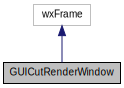
\includegraphics[width=196pt]{classGUICutRenderWindow__inherit__graph}
\end{center}
\end{figure}


Zusammengehörigkeiten von G\-U\-I\-Cut\-Render\-Window\-:\nopagebreak
\begin{figure}[H]
\begin{center}
\leavevmode
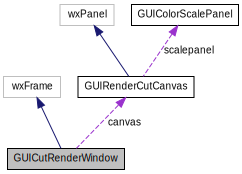
\includegraphics[width=314pt]{classGUICutRenderWindow__coll__graph}
\end{center}
\end{figure}
\subsection*{Öffentliche Methoden}
\begin{DoxyCompactItemize}
\item 
\hyperlink{classGUICutRenderWindow_ae522616f2d98dd3455a1d6dcc4ee877f}{G\-U\-I\-Cut\-Render\-Window} (wx\-Window $\ast$parent, const wx\-Char $\ast$title, int xpos, int ypos, int width, int height)
\item 
virtual \hyperlink{classGUICutRenderWindow_aced4a67c460b8c3ede40763b6da6953d}{$\sim$\-G\-U\-I\-Cut\-Render\-Window} ()
\end{DoxyCompactItemize}
\subsection*{Geschützte Methoden}
\begin{DoxyCompactItemize}
\item 
\hyperlink{classGUICutRenderWindow_a3eda2915b515c63309d996a9c1dc6442}{D\-E\-C\-L\-A\-R\-E\-\_\-\-E\-V\-E\-N\-T\-\_\-\-T\-A\-B\-L\-E} ()
\end{DoxyCompactItemize}
\subsection*{Private Methoden}
\begin{DoxyCompactItemize}
\item 
\hyperlink{structUtils_1_1CutRender__info}{Cut\-Render\-\_\-info} $\ast$ \hyperlink{classGUICutRenderWindow_a01c347a6ff7868df925e46e48fc1a289}{get\-Cut\-Render\-Properties} ()
\item 
void \hyperlink{classGUICutRenderWindow_a7cd1bfbec53756a1cbbe1616b4d46c7a}{render\-Cut\-Bt\-Click} (wx\-Command\-Event \&event)
\item 
void \hyperlink{classGUICutRenderWindow_ab57ff6c0d5e6465bb0f3b5cf0e6d9dc9}{On\-Resize} (wx\-Size\-Event \&event)
\item 
void \hyperlink{classGUICutRenderWindow_a780972413c43b3086e86c28d581d1f70}{On\-Cut\-Props\-Changed} (wx\-Command\-Event \&event)
\item 
void \hyperlink{classGUICutRenderWindow_a525891e3dde6ffd445bfed747dcee970}{refresh\-Visualisation} ()
\item 
void \hyperlink{classGUICutRenderWindow_a97f4602acc61f4b62c4d90ddbb692a25}{On\-Export\-Image} (wx\-Command\-Event \&event)
\item 
void \hyperlink{classGUICutRenderWindow_a3aee786d94c840ab4e6df6e3c2817802}{On\-Export\-C\-S\-V} (wx\-Command\-Event \&event)
\item 
void \hyperlink{classGUICutRenderWindow_a50e92af9db469de6d0298e58eee783ce}{On\-S\-Cut\-Props\-Changed\-\_\-spin} (wx\-Spin\-Event \&event)
\item 
void \hyperlink{classGUICutRenderWindow_a25feed7d1598253a25fc9c3bfe4131ec}{On\-Color\-Scale\-Changed} (wx\-Command\-Event \&event)
\item 
void \hyperlink{classGUICutRenderWindow_a3a2c47b00b30661632dae29eed266438}{On\-Color\-Scale\-Changed\-\_\-spin} (wx\-Spin\-Event \&event)
\item 
void \hyperlink{classGUICutRenderWindow_a0923a36cdf4e0094d78f623693ff8ac6}{On\-C\-S\-Color\-Bt\-Click} (wx\-Command\-Event \&event)
\item 
void \hyperlink{classGUICutRenderWindow_a9eedb7088ad31f4680a77ed3a06fa60c}{render\-Image} (wx\-Image $\ast$\hyperlink{classGUICutRenderWindow_a30c36db74a83fc5523407d3611c1db34}{image})
\end{DoxyCompactItemize}
\subsection*{Private Attribute}
\begin{DoxyCompactItemize}
\item 
wx\-Scrolled\-Window $\ast$ \hyperlink{classGUICutRenderWindow_a28c430f7145860ba3265fa9b8417923d}{scroll\-\_\-pane}
\item 
wx\-Text\-Ctrl $\ast$ \hyperlink{classGUICutRenderWindow_a509b5ca573c287e3863e952ec629fa7b}{p1xedit}
\item 
wx\-Text\-Ctrl $\ast$ \hyperlink{classGUICutRenderWindow_a93e837c15d8c6e7f420fd457c49024f2}{p1yedit}
\item 
wx\-Text\-Ctrl $\ast$ \hyperlink{classGUICutRenderWindow_a5843efcb13e1d56ea95932d052e5666a}{p1zedit}
\item 
wx\-Text\-Ctrl $\ast$ \hyperlink{classGUICutRenderWindow_a5d2bcd96c6fdb8d629583c5d40ccdbcc}{p2xedit}
\item 
wx\-Text\-Ctrl $\ast$ \hyperlink{classGUICutRenderWindow_a8ec4550ec7d30a8ad3c4c1e5dfcb8dce}{p2yedit}
\item 
wx\-Text\-Ctrl $\ast$ \hyperlink{classGUICutRenderWindow_affad4d5ff6cf42dd585a1a5f0e050075}{p2zedit}
\item 
wx\-Text\-Ctrl $\ast$ \hyperlink{classGUICutRenderWindow_a3382e7bd629988774c4f5e81bf66ca7e}{p3xedit}
\item 
wx\-Text\-Ctrl $\ast$ \hyperlink{classGUICutRenderWindow_a5f908b41a4d9db847cd89c0a3c52b61a}{p3yedit}
\item 
wx\-Text\-Ctrl $\ast$ \hyperlink{classGUICutRenderWindow_ac4c2f8825a9596f32093f0ac08a7848d}{p3zedit}
\item 
wx\-Spin\-Ctrl $\ast$ \hyperlink{classGUICutRenderWindow_a211043ba4bd60862a9fbfe1186c40875}{img\-Width\-Edit}
\item 
wx\-Spin\-Ctrl $\ast$ \hyperlink{classGUICutRenderWindow_a4daa569840f00756e6781ad2d87aef5b}{img\-Height\-Edit}
\item 
wx\-Spin\-Ctrl $\ast$ \hyperlink{classGUICutRenderWindow_ae48406dc8c80240904ca7040b7b3fbf1}{threadcountedit}
\item 
wx\-Text\-Ctrl $\ast$ \hyperlink{classGUICutRenderWindow_a76ced7f0bb7a2b08142aaf225f37c108}{mmperpixeledit}
\item 
wx\-Static\-Text $\ast$ \hyperlink{classGUICutRenderWindow_ac28961397f75c1d67dd1d983cda586f8}{p1label}
\item 
wx\-Static\-Text $\ast$ \hyperlink{classGUICutRenderWindow_adc1202b42f220ea7b8a8830f4d9d322a}{p2label}
\item 
wx\-Static\-Text $\ast$ \hyperlink{classGUICutRenderWindow_a6d1f742f0a78f84882f543f0cbbd6357}{p3label}
\item 
wx\-Static\-Text $\ast$ \hyperlink{classGUICutRenderWindow_ab1f4863c699e72e54e8b3f6d320a5e3a}{mmperpixellabel}
\item 
wx\-Static\-Text $\ast$ \hyperlink{classGUICutRenderWindow_a1d6dae72dbc65725dee34799e7fb7af1}{trilabel}
\item 
wx\-Static\-Text $\ast$ \hyperlink{classGUICutRenderWindow_a3317d0e8526d4a11168e86f673576ee3}{optionslbl}
\item 
wx\-Static\-Text $\ast$ \hyperlink{classGUICutRenderWindow_a26632978654028e6fbfaa6eef704ff06}{width\-Heightlbl}
\item 
wx\-Static\-Text $\ast$ \hyperlink{classGUICutRenderWindow_a2797a52c219092ce3f54ea62ec4b95f3}{threadcountlbl}
\item 
wx\-Static\-Text $\ast$ \hyperlink{classGUICutRenderWindow_a3c1e80a372d6eaacd4f6ca71a788c9fd}{scalelbl}
\item 
wx\-Static\-Text $\ast$ \hyperlink{classGUICutRenderWindow_a2a3f0b64122aff2f336f94fb72b3b8ac}{scalemodelbl}
\item 
wx\-Combo\-Box $\ast$ \hyperlink{classGUICutRenderWindow_af535e1e80e14178ff5c05707261a183d}{scalemodecb}
\item 
wx\-Static\-Text $\ast$ \hyperlink{classGUICutRenderWindow_a1f46a30a61ad94b76a6194758bdb3f95}{scalefontpropslbl}
\item 
wx\-Spin\-Ctrl $\ast$ \hyperlink{classGUICutRenderWindow_a62cb232f5f9747c1fdbc5c1f6ff4b7a4}{scalefontsizeedit}
\item 
wx\-Button $\ast$ \hyperlink{classGUICutRenderWindow_a13a1557216de339d20189fdaa0df482b}{scalefontcolorbt}
\item 
wx\-Spin\-Ctrl $\ast$ \hyperlink{classGUICutRenderWindow_a4fbe9115e418be48a70eff31e94640ba}{scalestepedit}
\item 
wx\-Button $\ast$ \hyperlink{classGUICutRenderWindow_a7cadc8f5fd1b153ba21aa82fd5f70eff}{calcbt}
\item 
wx\-Button $\ast$ \hyperlink{classGUICutRenderWindow_ac0b26b746d6339154256d81da8cd7aed}{export\-\_\-img\-\_\-bt}
\item 
wx\-Button $\ast$ \hyperlink{classGUICutRenderWindow_a1613155eefe8309903858f9427b263de}{export\-\_\-csv\-\_\-bt}
\item 
\hyperlink{classGUIRenderCutCanvas}{G\-U\-I\-Render\-Cut\-Canvas} $\ast$ \hyperlink{classGUICutRenderWindow_abbaa6c66e8aa9fee96ba20a9a29e1a18}{canvas}
\item 
wx\-Image $\ast$ \hyperlink{classGUICutRenderWindow_a30c36db74a83fc5523407d3611c1db34}{image}
\item 
float $\ast$ \hyperlink{classGUICutRenderWindow_a9c8338a733363aea25a8735d6873a414}{value\-\_\-img}
\item 
int \hyperlink{classGUICutRenderWindow_a365103460aeafd2173c0a9360cc0caa1}{core\-\_\-count}
\end{DoxyCompactItemize}


\subsection{Ausführliche Beschreibung}
Fenster zum erstellen zweidimensionaler Temperaturverteilungen. 

Das Fenster ermöglicht es, eine zweidimensionale Temperaturverteilung auf einer Schnittebene durch das dreidimensionale Modell zu berechnen. Diese Schnittebene wird im 3\-D-\/\-Fenster des Hauptfensters visualisiert. 

Definiert in Zeile 24 der Datei G\-U\-I\-Cut\-Render\-Window.\-h.



\subsection{Beschreibung der Konstruktoren und Destruktoren}
\hypertarget{classGUICutRenderWindow_ae522616f2d98dd3455a1d6dcc4ee877f}{\index{G\-U\-I\-Cut\-Render\-Window@{G\-U\-I\-Cut\-Render\-Window}!G\-U\-I\-Cut\-Render\-Window@{G\-U\-I\-Cut\-Render\-Window}}
\index{G\-U\-I\-Cut\-Render\-Window@{G\-U\-I\-Cut\-Render\-Window}!GUICutRenderWindow@{G\-U\-I\-Cut\-Render\-Window}}
\subsubsection[{G\-U\-I\-Cut\-Render\-Window}]{\setlength{\rightskip}{0pt plus 5cm}G\-U\-I\-Cut\-Render\-Window\-::\-G\-U\-I\-Cut\-Render\-Window (
\begin{DoxyParamCaption}
\item[{wx\-Window $\ast$}]{parent, }
\item[{const wx\-Char $\ast$}]{title, }
\item[{int}]{xpos, }
\item[{int}]{ypos, }
\item[{int}]{width, }
\item[{int}]{height}
\end{DoxyParamCaption}
)}}\label{classGUICutRenderWindow_ae522616f2d98dd3455a1d6dcc4ee877f}
Der Konstuktor. 
\begin{DoxyParams}{Parameter}
{\em parent} & Das Übergeordnete Fenster. Muss vom Typ \hyperlink{classGUIMainWindow}{G\-U\-I\-Main\-Window} sein. \\
\hline
{\em title} & Titel des Fensters. \\
\hline
{\em xpos} & horizontale Position des Fensters. \\
\hline
{\em ypos} & vertikale Position des Fensters. \\
\hline
{\em width} & Breite des Fensters. \\
\hline
{\em height} & Höhe des Fenster \\
\hline
\end{DoxyParams}


Definiert in Zeile 37 der Datei G\-U\-I\-Cut\-Render\-Window.\-cpp.

\hypertarget{classGUICutRenderWindow_aced4a67c460b8c3ede40763b6da6953d}{\index{G\-U\-I\-Cut\-Render\-Window@{G\-U\-I\-Cut\-Render\-Window}!$\sim$\-G\-U\-I\-Cut\-Render\-Window@{$\sim$\-G\-U\-I\-Cut\-Render\-Window}}
\index{$\sim$\-G\-U\-I\-Cut\-Render\-Window@{$\sim$\-G\-U\-I\-Cut\-Render\-Window}!GUICutRenderWindow@{G\-U\-I\-Cut\-Render\-Window}}
\subsubsection[{$\sim$\-G\-U\-I\-Cut\-Render\-Window}]{\setlength{\rightskip}{0pt plus 5cm}G\-U\-I\-Cut\-Render\-Window\-::$\sim$\-G\-U\-I\-Cut\-Render\-Window (
\begin{DoxyParamCaption}
{}
\end{DoxyParamCaption}
)\hspace{0.3cm}{\ttfamily [virtual]}}}\label{classGUICutRenderWindow_aced4a67c460b8c3ede40763b6da6953d}
Der Destruktor. 

Definiert in Zeile 367 der Datei G\-U\-I\-Cut\-Render\-Window.\-cpp.



Hier ist ein Graph, der zeigt, was diese Funktion aufruft\-:\nopagebreak
\begin{figure}[H]
\begin{center}
\leavevmode
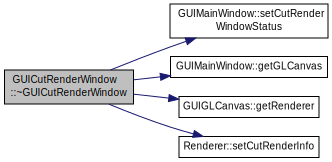
\includegraphics[width=350pt]{classGUICutRenderWindow_aced4a67c460b8c3ede40763b6da6953d_cgraph}
\end{center}
\end{figure}




\subsection{Dokumentation der Elementfunktionen}
\hypertarget{classGUICutRenderWindow_a3eda2915b515c63309d996a9c1dc6442}{\index{G\-U\-I\-Cut\-Render\-Window@{G\-U\-I\-Cut\-Render\-Window}!D\-E\-C\-L\-A\-R\-E\-\_\-\-E\-V\-E\-N\-T\-\_\-\-T\-A\-B\-L\-E@{D\-E\-C\-L\-A\-R\-E\-\_\-\-E\-V\-E\-N\-T\-\_\-\-T\-A\-B\-L\-E}}
\index{D\-E\-C\-L\-A\-R\-E\-\_\-\-E\-V\-E\-N\-T\-\_\-\-T\-A\-B\-L\-E@{D\-E\-C\-L\-A\-R\-E\-\_\-\-E\-V\-E\-N\-T\-\_\-\-T\-A\-B\-L\-E}!GUICutRenderWindow@{G\-U\-I\-Cut\-Render\-Window}}
\subsubsection[{D\-E\-C\-L\-A\-R\-E\-\_\-\-E\-V\-E\-N\-T\-\_\-\-T\-A\-B\-L\-E}]{\setlength{\rightskip}{0pt plus 5cm}G\-U\-I\-Cut\-Render\-Window\-::\-D\-E\-C\-L\-A\-R\-E\-\_\-\-E\-V\-E\-N\-T\-\_\-\-T\-A\-B\-L\-E (
\begin{DoxyParamCaption}
{}
\end{DoxyParamCaption}
)\hspace{0.3cm}{\ttfamily [protected]}}}\label{classGUICutRenderWindow_a3eda2915b515c63309d996a9c1dc6442}
Event-\/\-Tabellendeklaration für wx\-Widgets. \hypertarget{classGUICutRenderWindow_a01c347a6ff7868df925e46e48fc1a289}{\index{G\-U\-I\-Cut\-Render\-Window@{G\-U\-I\-Cut\-Render\-Window}!get\-Cut\-Render\-Properties@{get\-Cut\-Render\-Properties}}
\index{get\-Cut\-Render\-Properties@{get\-Cut\-Render\-Properties}!GUICutRenderWindow@{G\-U\-I\-Cut\-Render\-Window}}
\subsubsection[{get\-Cut\-Render\-Properties}]{\setlength{\rightskip}{0pt plus 5cm}{\bf Cut\-Render\-\_\-info} $\ast$ G\-U\-I\-Cut\-Render\-Window\-::get\-Cut\-Render\-Properties (
\begin{DoxyParamCaption}
{}
\end{DoxyParamCaption}
)\hspace{0.3cm}{\ttfamily [private]}}}\label{classGUICutRenderWindow_a01c347a6ff7868df925e46e48fc1a289}
Gibt die aktuell eingestellten Eigenschaften für die zweidimensionale Temperaturverteilung zurück, damit Sie später an den \hyperlink{classRenderer}{Renderer} des 3\-D-\/\-Fensters zur Visualisierung übergeben werden können. 

Definiert in Zeile 329 der Datei G\-U\-I\-Cut\-Render\-Window.\-cpp.



Hier ist ein Graph der zeigt, wo diese Funktion aufgerufen wird\-:\nopagebreak
\begin{figure}[H]
\begin{center}
\leavevmode
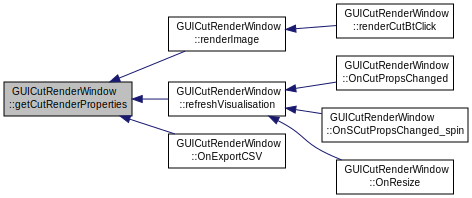
\includegraphics[width=350pt]{classGUICutRenderWindow_a01c347a6ff7868df925e46e48fc1a289_icgraph}
\end{center}
\end{figure}


\hypertarget{classGUICutRenderWindow_a25feed7d1598253a25fc9c3bfe4131ec}{\index{G\-U\-I\-Cut\-Render\-Window@{G\-U\-I\-Cut\-Render\-Window}!On\-Color\-Scale\-Changed@{On\-Color\-Scale\-Changed}}
\index{On\-Color\-Scale\-Changed@{On\-Color\-Scale\-Changed}!GUICutRenderWindow@{G\-U\-I\-Cut\-Render\-Window}}
\subsubsection[{On\-Color\-Scale\-Changed}]{\setlength{\rightskip}{0pt plus 5cm}void G\-U\-I\-Cut\-Render\-Window\-::\-On\-Color\-Scale\-Changed (
\begin{DoxyParamCaption}
\item[{wx\-Command\-Event \&}]{event}
\end{DoxyParamCaption}
)\hspace{0.3cm}{\ttfamily [private]}}}\label{classGUICutRenderWindow_a25feed7d1598253a25fc9c3bfe4131ec}
Behandelt das Ändern von Parametern zur darstellung der Temperaturskala. 

Definiert in Zeile 354 der Datei G\-U\-I\-Cut\-Render\-Window.\-cpp.



Hier ist ein Graph, der zeigt, was diese Funktion aufruft\-:
\nopagebreak
\begin{figure}[H]
\begin{center}
\leavevmode
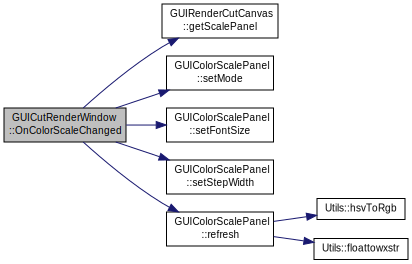
\includegraphics[width=350pt]{classGUICutRenderWindow_a25feed7d1598253a25fc9c3bfe4131ec_cgraph}
\end{center}
\end{figure}




Hier ist ein Graph der zeigt, wo diese Funktion aufgerufen wird\-:\nopagebreak
\begin{figure}[H]
\begin{center}
\leavevmode
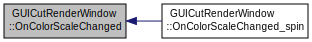
\includegraphics[width=350pt]{classGUICutRenderWindow_a25feed7d1598253a25fc9c3bfe4131ec_icgraph}
\end{center}
\end{figure}


\hypertarget{classGUICutRenderWindow_a3a2c47b00b30661632dae29eed266438}{\index{G\-U\-I\-Cut\-Render\-Window@{G\-U\-I\-Cut\-Render\-Window}!On\-Color\-Scale\-Changed\-\_\-spin@{On\-Color\-Scale\-Changed\-\_\-spin}}
\index{On\-Color\-Scale\-Changed\-\_\-spin@{On\-Color\-Scale\-Changed\-\_\-spin}!GUICutRenderWindow@{G\-U\-I\-Cut\-Render\-Window}}
\subsubsection[{On\-Color\-Scale\-Changed\-\_\-spin}]{\setlength{\rightskip}{0pt plus 5cm}void G\-U\-I\-Cut\-Render\-Window\-::\-On\-Color\-Scale\-Changed\-\_\-spin (
\begin{DoxyParamCaption}
\item[{wx\-Spin\-Event \&}]{event}
\end{DoxyParamCaption}
)\hspace{0.3cm}{\ttfamily [private]}}}\label{classGUICutRenderWindow_a3a2c47b00b30661632dae29eed266438}
Behandelt das Ändern von Parametern zur darstellung der Temperaturskala. 

Definiert in Zeile 341 der Datei G\-U\-I\-Cut\-Render\-Window.\-cpp.



Hier ist ein Graph, der zeigt, was diese Funktion aufruft\-:
\nopagebreak
\begin{figure}[H]
\begin{center}
\leavevmode
\includegraphics[width=350pt]{classGUICutRenderWindow_a3a2c47b00b30661632dae29eed266438_cgraph}
\end{center}
\end{figure}


\hypertarget{classGUICutRenderWindow_a0923a36cdf4e0094d78f623693ff8ac6}{\index{G\-U\-I\-Cut\-Render\-Window@{G\-U\-I\-Cut\-Render\-Window}!On\-C\-S\-Color\-Bt\-Click@{On\-C\-S\-Color\-Bt\-Click}}
\index{On\-C\-S\-Color\-Bt\-Click@{On\-C\-S\-Color\-Bt\-Click}!GUICutRenderWindow@{G\-U\-I\-Cut\-Render\-Window}}
\subsubsection[{On\-C\-S\-Color\-Bt\-Click}]{\setlength{\rightskip}{0pt plus 5cm}void G\-U\-I\-Cut\-Render\-Window\-::\-On\-C\-S\-Color\-Bt\-Click (
\begin{DoxyParamCaption}
\item[{wx\-Command\-Event \&}]{event}
\end{DoxyParamCaption}
)\hspace{0.3cm}{\ttfamily [private]}}}\label{classGUICutRenderWindow_a0923a36cdf4e0094d78f623693ff8ac6}
Behandelt das Klicken auf den Button zur Wahl der Schriftfarbe auf der Skala. 

Definiert in Zeile 345 der Datei G\-U\-I\-Cut\-Render\-Window.\-cpp.



Hier ist ein Graph, der zeigt, was diese Funktion aufruft\-:
\nopagebreak
\begin{figure}[H]
\begin{center}
\leavevmode
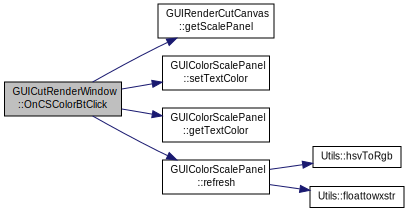
\includegraphics[width=350pt]{classGUICutRenderWindow_a0923a36cdf4e0094d78f623693ff8ac6_cgraph}
\end{center}
\end{figure}


\hypertarget{classGUICutRenderWindow_a780972413c43b3086e86c28d581d1f70}{\index{G\-U\-I\-Cut\-Render\-Window@{G\-U\-I\-Cut\-Render\-Window}!On\-Cut\-Props\-Changed@{On\-Cut\-Props\-Changed}}
\index{On\-Cut\-Props\-Changed@{On\-Cut\-Props\-Changed}!GUICutRenderWindow@{G\-U\-I\-Cut\-Render\-Window}}
\subsubsection[{On\-Cut\-Props\-Changed}]{\setlength{\rightskip}{0pt plus 5cm}void G\-U\-I\-Cut\-Render\-Window\-::\-On\-Cut\-Props\-Changed (
\begin{DoxyParamCaption}
\item[{wx\-Command\-Event \&}]{event}
\end{DoxyParamCaption}
)\hspace{0.3cm}{\ttfamily [private]}}}\label{classGUICutRenderWindow_a780972413c43b3086e86c28d581d1f70}
Behandelt das Ändern von Parametern zur Berechnung der 2\-D-\/\-Temperaturverteilung. 

Definiert in Zeile 240 der Datei G\-U\-I\-Cut\-Render\-Window.\-cpp.



Hier ist ein Graph, der zeigt, was diese Funktion aufruft\-:\nopagebreak
\begin{figure}[H]
\begin{center}
\leavevmode
\includegraphics[width=350pt]{classGUICutRenderWindow_a780972413c43b3086e86c28d581d1f70_cgraph}
\end{center}
\end{figure}


\hypertarget{classGUICutRenderWindow_a3aee786d94c840ab4e6df6e3c2817802}{\index{G\-U\-I\-Cut\-Render\-Window@{G\-U\-I\-Cut\-Render\-Window}!On\-Export\-C\-S\-V@{On\-Export\-C\-S\-V}}
\index{On\-Export\-C\-S\-V@{On\-Export\-C\-S\-V}!GUICutRenderWindow@{G\-U\-I\-Cut\-Render\-Window}}
\subsubsection[{On\-Export\-C\-S\-V}]{\setlength{\rightskip}{0pt plus 5cm}void G\-U\-I\-Cut\-Render\-Window\-::\-On\-Export\-C\-S\-V (
\begin{DoxyParamCaption}
\item[{wx\-Command\-Event \&}]{event}
\end{DoxyParamCaption}
)\hspace{0.3cm}{\ttfamily [private]}}}\label{classGUICutRenderWindow_a3aee786d94c840ab4e6df6e3c2817802}
Fragt den Benutzer nach dem Pfad und Exporiert die 2\-D-\/\-Temperaturverteilung als .csv-\/\-Datei. 

Definiert in Zeile 293 der Datei G\-U\-I\-Cut\-Render\-Window.\-cpp.



Hier ist ein Graph, der zeigt, was diese Funktion aufruft\-:\nopagebreak
\begin{figure}[H]
\begin{center}
\leavevmode
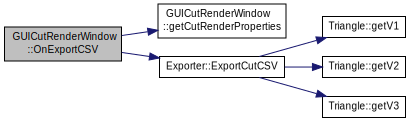
\includegraphics[width=350pt]{classGUICutRenderWindow_a3aee786d94c840ab4e6df6e3c2817802_cgraph}
\end{center}
\end{figure}


\hypertarget{classGUICutRenderWindow_a97f4602acc61f4b62c4d90ddbb692a25}{\index{G\-U\-I\-Cut\-Render\-Window@{G\-U\-I\-Cut\-Render\-Window}!On\-Export\-Image@{On\-Export\-Image}}
\index{On\-Export\-Image@{On\-Export\-Image}!GUICutRenderWindow@{G\-U\-I\-Cut\-Render\-Window}}
\subsubsection[{On\-Export\-Image}]{\setlength{\rightskip}{0pt plus 5cm}void G\-U\-I\-Cut\-Render\-Window\-::\-On\-Export\-Image (
\begin{DoxyParamCaption}
\item[{wx\-Command\-Event \&}]{event}
\end{DoxyParamCaption}
)\hspace{0.3cm}{\ttfamily [private]}}}\label{classGUICutRenderWindow_a97f4602acc61f4b62c4d90ddbb692a25}
Fragt den Benutzer nach dem Pfad und Exporiert eine Grafik aus 2\-D-\/\-Temperaturverteilung und Temperaturskala. 

Definiert in Zeile 306 der Datei G\-U\-I\-Cut\-Render\-Window.\-cpp.



Hier ist ein Graph, der zeigt, was diese Funktion aufruft\-:\nopagebreak
\begin{figure}[H]
\begin{center}
\leavevmode
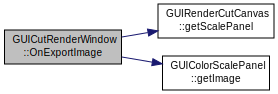
\includegraphics[width=350pt]{classGUICutRenderWindow_a97f4602acc61f4b62c4d90ddbb692a25_cgraph}
\end{center}
\end{figure}


\hypertarget{classGUICutRenderWindow_ab57ff6c0d5e6465bb0f3b5cf0e6d9dc9}{\index{G\-U\-I\-Cut\-Render\-Window@{G\-U\-I\-Cut\-Render\-Window}!On\-Resize@{On\-Resize}}
\index{On\-Resize@{On\-Resize}!GUICutRenderWindow@{G\-U\-I\-Cut\-Render\-Window}}
\subsubsection[{On\-Resize}]{\setlength{\rightskip}{0pt plus 5cm}void G\-U\-I\-Cut\-Render\-Window\-::\-On\-Resize (
\begin{DoxyParamCaption}
\item[{wx\-Size\-Event \&}]{event}
\end{DoxyParamCaption}
)\hspace{0.3cm}{\ttfamily [private]}}}\label{classGUICutRenderWindow_ab57ff6c0d5e6465bb0f3b5cf0e6d9dc9}
Behandelt Änderungen der Größe des Fensters. 

Definiert in Zeile 251 der Datei G\-U\-I\-Cut\-Render\-Window.\-cpp.



Hier ist ein Graph, der zeigt, was diese Funktion aufruft\-:\nopagebreak
\begin{figure}[H]
\begin{center}
\leavevmode
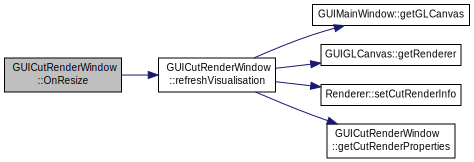
\includegraphics[width=350pt]{classGUICutRenderWindow_ab57ff6c0d5e6465bb0f3b5cf0e6d9dc9_cgraph}
\end{center}
\end{figure}


\hypertarget{classGUICutRenderWindow_a50e92af9db469de6d0298e58eee783ce}{\index{G\-U\-I\-Cut\-Render\-Window@{G\-U\-I\-Cut\-Render\-Window}!On\-S\-Cut\-Props\-Changed\-\_\-spin@{On\-S\-Cut\-Props\-Changed\-\_\-spin}}
\index{On\-S\-Cut\-Props\-Changed\-\_\-spin@{On\-S\-Cut\-Props\-Changed\-\_\-spin}!GUICutRenderWindow@{G\-U\-I\-Cut\-Render\-Window}}
\subsubsection[{On\-S\-Cut\-Props\-Changed\-\_\-spin}]{\setlength{\rightskip}{0pt plus 5cm}void G\-U\-I\-Cut\-Render\-Window\-::\-On\-S\-Cut\-Props\-Changed\-\_\-spin (
\begin{DoxyParamCaption}
\item[{wx\-Spin\-Event \&}]{event}
\end{DoxyParamCaption}
)\hspace{0.3cm}{\ttfamily [private]}}}\label{classGUICutRenderWindow_a50e92af9db469de6d0298e58eee783ce}
Behandelt das Ändern von Parametern zur Berechnung der 2\-D-\/\-Temperaturverteilung. 

Definiert in Zeile 243 der Datei G\-U\-I\-Cut\-Render\-Window.\-cpp.



Hier ist ein Graph, der zeigt, was diese Funktion aufruft\-:\nopagebreak
\begin{figure}[H]
\begin{center}
\leavevmode
\includegraphics[width=350pt]{classGUICutRenderWindow_a50e92af9db469de6d0298e58eee783ce_cgraph}
\end{center}
\end{figure}


\hypertarget{classGUICutRenderWindow_a525891e3dde6ffd445bfed747dcee970}{\index{G\-U\-I\-Cut\-Render\-Window@{G\-U\-I\-Cut\-Render\-Window}!refresh\-Visualisation@{refresh\-Visualisation}}
\index{refresh\-Visualisation@{refresh\-Visualisation}!GUICutRenderWindow@{G\-U\-I\-Cut\-Render\-Window}}
\subsubsection[{refresh\-Visualisation}]{\setlength{\rightskip}{0pt plus 5cm}void G\-U\-I\-Cut\-Render\-Window\-::refresh\-Visualisation (
\begin{DoxyParamCaption}
{}
\end{DoxyParamCaption}
)\hspace{0.3cm}{\ttfamily [private]}}}\label{classGUICutRenderWindow_a525891e3dde6ffd445bfed747dcee970}
Aktualisiert die Visualisierung der Schnittebene im Hauptfenster. 

Definiert in Zeile 246 der Datei G\-U\-I\-Cut\-Render\-Window.\-cpp.



Hier ist ein Graph, der zeigt, was diese Funktion aufruft\-:\nopagebreak
\begin{figure}[H]
\begin{center}
\leavevmode
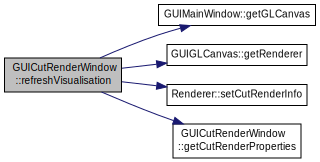
\includegraphics[width=350pt]{classGUICutRenderWindow_a525891e3dde6ffd445bfed747dcee970_cgraph}
\end{center}
\end{figure}




Hier ist ein Graph der zeigt, wo diese Funktion aufgerufen wird\-:\nopagebreak
\begin{figure}[H]
\begin{center}
\leavevmode
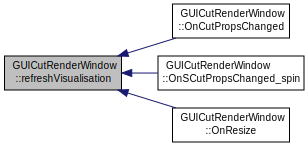
\includegraphics[width=350pt]{classGUICutRenderWindow_a525891e3dde6ffd445bfed747dcee970_icgraph}
\end{center}
\end{figure}


\hypertarget{classGUICutRenderWindow_a7cd1bfbec53756a1cbbe1616b4d46c7a}{\index{G\-U\-I\-Cut\-Render\-Window@{G\-U\-I\-Cut\-Render\-Window}!render\-Cut\-Bt\-Click@{render\-Cut\-Bt\-Click}}
\index{render\-Cut\-Bt\-Click@{render\-Cut\-Bt\-Click}!GUICutRenderWindow@{G\-U\-I\-Cut\-Render\-Window}}
\subsubsection[{render\-Cut\-Bt\-Click}]{\setlength{\rightskip}{0pt plus 5cm}void G\-U\-I\-Cut\-Render\-Window\-::render\-Cut\-Bt\-Click (
\begin{DoxyParamCaption}
\item[{wx\-Command\-Event \&}]{event}
\end{DoxyParamCaption}
)\hspace{0.3cm}{\ttfamily [private]}}}\label{classGUICutRenderWindow_a7cd1bfbec53756a1cbbe1616b4d46c7a}
Behandelt das Drücken des Buttons zur Berechnung der zweidimensionalen Temperaturverteilung. 

Definiert in Zeile 362 der Datei G\-U\-I\-Cut\-Render\-Window.\-cpp.



Hier ist ein Graph, der zeigt, was diese Funktion aufruft\-:
\nopagebreak
\begin{figure}[H]
\begin{center}
\leavevmode
\includegraphics[width=350pt]{classGUICutRenderWindow_a7cd1bfbec53756a1cbbe1616b4d46c7a_cgraph}
\end{center}
\end{figure}


\hypertarget{classGUICutRenderWindow_a9eedb7088ad31f4680a77ed3a06fa60c}{\index{G\-U\-I\-Cut\-Render\-Window@{G\-U\-I\-Cut\-Render\-Window}!render\-Image@{render\-Image}}
\index{render\-Image@{render\-Image}!GUICutRenderWindow@{G\-U\-I\-Cut\-Render\-Window}}
\subsubsection[{render\-Image}]{\setlength{\rightskip}{0pt plus 5cm}void G\-U\-I\-Cut\-Render\-Window\-::render\-Image (
\begin{DoxyParamCaption}
\item[{wx\-Image $\ast$}]{image}
\end{DoxyParamCaption}
)\hspace{0.3cm}{\ttfamily [private]}}}\label{classGUICutRenderWindow_a9eedb7088ad31f4680a77ed3a06fa60c}
Berechnet die 2\-D-\/\-Temperaturverteilung als Grafik. 

Definiert in Zeile 149 der Datei G\-U\-I\-Cut\-Render\-Window.\-cpp.



Hier ist ein Graph, der zeigt, was diese Funktion aufruft\-:
\nopagebreak
\begin{figure}[H]
\begin{center}
\leavevmode
\includegraphics[width=350pt]{classGUICutRenderWindow_a9eedb7088ad31f4680a77ed3a06fa60c_cgraph}
\end{center}
\end{figure}




Hier ist ein Graph der zeigt, wo diese Funktion aufgerufen wird\-:\nopagebreak
\begin{figure}[H]
\begin{center}
\leavevmode
\includegraphics[width=350pt]{classGUICutRenderWindow_a9eedb7088ad31f4680a77ed3a06fa60c_icgraph}
\end{center}
\end{figure}




\subsection{Dokumentation der Datenelemente}
\hypertarget{classGUICutRenderWindow_a7cadc8f5fd1b153ba21aa82fd5f70eff}{\index{G\-U\-I\-Cut\-Render\-Window@{G\-U\-I\-Cut\-Render\-Window}!calcbt@{calcbt}}
\index{calcbt@{calcbt}!GUICutRenderWindow@{G\-U\-I\-Cut\-Render\-Window}}
\subsubsection[{calcbt}]{\setlength{\rightskip}{0pt plus 5cm}wx\-Button$\ast$ G\-U\-I\-Cut\-Render\-Window\-::calcbt\hspace{0.3cm}{\ttfamily [private]}}}\label{classGUICutRenderWindow_a7cadc8f5fd1b153ba21aa82fd5f70eff}
Button zum Starten der Berechnung der 2\-D-\/\-Temperaturverteilung. 

Definiert in Zeile 214 der Datei G\-U\-I\-Cut\-Render\-Window.\-h.

\hypertarget{classGUICutRenderWindow_abbaa6c66e8aa9fee96ba20a9a29e1a18}{\index{G\-U\-I\-Cut\-Render\-Window@{G\-U\-I\-Cut\-Render\-Window}!canvas@{canvas}}
\index{canvas@{canvas}!GUICutRenderWindow@{G\-U\-I\-Cut\-Render\-Window}}
\subsubsection[{canvas}]{\setlength{\rightskip}{0pt plus 5cm}{\bf G\-U\-I\-Render\-Cut\-Canvas}$\ast$ G\-U\-I\-Cut\-Render\-Window\-::canvas\hspace{0.3cm}{\ttfamily [private]}}}\label{classGUICutRenderWindow_abbaa6c66e8aa9fee96ba20a9a29e1a18}
Die Zeichenfläche zur Darstellung der berechneten Grafik und der Skala. 

Definiert in Zeile 226 der Datei G\-U\-I\-Cut\-Render\-Window.\-h.

\hypertarget{classGUICutRenderWindow_a365103460aeafd2173c0a9360cc0caa1}{\index{G\-U\-I\-Cut\-Render\-Window@{G\-U\-I\-Cut\-Render\-Window}!core\-\_\-count@{core\-\_\-count}}
\index{core\-\_\-count@{core\-\_\-count}!GUICutRenderWindow@{G\-U\-I\-Cut\-Render\-Window}}
\subsubsection[{core\-\_\-count}]{\setlength{\rightskip}{0pt plus 5cm}int G\-U\-I\-Cut\-Render\-Window\-::core\-\_\-count\hspace{0.3cm}{\ttfamily [private]}}}\label{classGUICutRenderWindow_a365103460aeafd2173c0a9360cc0caa1}
Die Anzahl der zu bei der Berechnung zu verwendender Prozessorkerne. 

Definiert in Zeile 238 der Datei G\-U\-I\-Cut\-Render\-Window.\-h.

\hypertarget{classGUICutRenderWindow_a1613155eefe8309903858f9427b263de}{\index{G\-U\-I\-Cut\-Render\-Window@{G\-U\-I\-Cut\-Render\-Window}!export\-\_\-csv\-\_\-bt@{export\-\_\-csv\-\_\-bt}}
\index{export\-\_\-csv\-\_\-bt@{export\-\_\-csv\-\_\-bt}!GUICutRenderWindow@{G\-U\-I\-Cut\-Render\-Window}}
\subsubsection[{export\-\_\-csv\-\_\-bt}]{\setlength{\rightskip}{0pt plus 5cm}wx\-Button$\ast$ G\-U\-I\-Cut\-Render\-Window\-::export\-\_\-csv\-\_\-bt\hspace{0.3cm}{\ttfamily [private]}}}\label{classGUICutRenderWindow_a1613155eefe8309903858f9427b263de}
Button zum Export der Temperaturverteilung als .csv-\/\-Datei. 

Definiert in Zeile 222 der Datei G\-U\-I\-Cut\-Render\-Window.\-h.

\hypertarget{classGUICutRenderWindow_ac0b26b746d6339154256d81da8cd7aed}{\index{G\-U\-I\-Cut\-Render\-Window@{G\-U\-I\-Cut\-Render\-Window}!export\-\_\-img\-\_\-bt@{export\-\_\-img\-\_\-bt}}
\index{export\-\_\-img\-\_\-bt@{export\-\_\-img\-\_\-bt}!GUICutRenderWindow@{G\-U\-I\-Cut\-Render\-Window}}
\subsubsection[{export\-\_\-img\-\_\-bt}]{\setlength{\rightskip}{0pt plus 5cm}wx\-Button$\ast$ G\-U\-I\-Cut\-Render\-Window\-::export\-\_\-img\-\_\-bt\hspace{0.3cm}{\ttfamily [private]}}}\label{classGUICutRenderWindow_ac0b26b746d6339154256d81da8cd7aed}
Button zum Export der Grafik. 

Definiert in Zeile 218 der Datei G\-U\-I\-Cut\-Render\-Window.\-h.

\hypertarget{classGUICutRenderWindow_a30c36db74a83fc5523407d3611c1db34}{\index{G\-U\-I\-Cut\-Render\-Window@{G\-U\-I\-Cut\-Render\-Window}!image@{image}}
\index{image@{image}!GUICutRenderWindow@{G\-U\-I\-Cut\-Render\-Window}}
\subsubsection[{image}]{\setlength{\rightskip}{0pt plus 5cm}wx\-Image$\ast$ G\-U\-I\-Cut\-Render\-Window\-::image\hspace{0.3cm}{\ttfamily [private]}}}\label{classGUICutRenderWindow_a30c36db74a83fc5523407d3611c1db34}
Die berechnete Temperaturverteilung als Grafik. 

Definiert in Zeile 230 der Datei G\-U\-I\-Cut\-Render\-Window.\-h.

\hypertarget{classGUICutRenderWindow_a4daa569840f00756e6781ad2d87aef5b}{\index{G\-U\-I\-Cut\-Render\-Window@{G\-U\-I\-Cut\-Render\-Window}!img\-Height\-Edit@{img\-Height\-Edit}}
\index{img\-Height\-Edit@{img\-Height\-Edit}!GUICutRenderWindow@{G\-U\-I\-Cut\-Render\-Window}}
\subsubsection[{img\-Height\-Edit}]{\setlength{\rightskip}{0pt plus 5cm}wx\-Spin\-Ctrl$\ast$ G\-U\-I\-Cut\-Render\-Window\-::img\-Height\-Edit\hspace{0.3cm}{\ttfamily [private]}}}\label{classGUICutRenderWindow_a4daa569840f00756e6781ad2d87aef5b}
Feld zur Eingabe der Höhe des Bereichs, für den die 2\-D-\/\-Temperaturverteilung als Grafik berechnet wird. 

Definiert in Zeile 142 der Datei G\-U\-I\-Cut\-Render\-Window.\-h.

\hypertarget{classGUICutRenderWindow_a211043ba4bd60862a9fbfe1186c40875}{\index{G\-U\-I\-Cut\-Render\-Window@{G\-U\-I\-Cut\-Render\-Window}!img\-Width\-Edit@{img\-Width\-Edit}}
\index{img\-Width\-Edit@{img\-Width\-Edit}!GUICutRenderWindow@{G\-U\-I\-Cut\-Render\-Window}}
\subsubsection[{img\-Width\-Edit}]{\setlength{\rightskip}{0pt plus 5cm}wx\-Spin\-Ctrl$\ast$ G\-U\-I\-Cut\-Render\-Window\-::img\-Width\-Edit\hspace{0.3cm}{\ttfamily [private]}}}\label{classGUICutRenderWindow_a211043ba4bd60862a9fbfe1186c40875}
Textfeld zur Eingabe der Breite des Bereichs, für den die 2\-D-\/\-Temperaturverteilung als Grafik berechnet wird. 

Definiert in Zeile 138 der Datei G\-U\-I\-Cut\-Render\-Window.\-h.

\hypertarget{classGUICutRenderWindow_a76ced7f0bb7a2b08142aaf225f37c108}{\index{G\-U\-I\-Cut\-Render\-Window@{G\-U\-I\-Cut\-Render\-Window}!mmperpixeledit@{mmperpixeledit}}
\index{mmperpixeledit@{mmperpixeledit}!GUICutRenderWindow@{G\-U\-I\-Cut\-Render\-Window}}
\subsubsection[{mmperpixeledit}]{\setlength{\rightskip}{0pt plus 5cm}wx\-Text\-Ctrl$\ast$ G\-U\-I\-Cut\-Render\-Window\-::mmperpixeledit\hspace{0.3cm}{\ttfamily [private]}}}\label{classGUICutRenderWindow_a76ced7f0bb7a2b08142aaf225f37c108}
Feld zur Eingabe des Maßstabs in $\frac{mm}{px}$. 

Definiert in Zeile 150 der Datei G\-U\-I\-Cut\-Render\-Window.\-h.

\hypertarget{classGUICutRenderWindow_ab1f4863c699e72e54e8b3f6d320a5e3a}{\index{G\-U\-I\-Cut\-Render\-Window@{G\-U\-I\-Cut\-Render\-Window}!mmperpixellabel@{mmperpixellabel}}
\index{mmperpixellabel@{mmperpixellabel}!GUICutRenderWindow@{G\-U\-I\-Cut\-Render\-Window}}
\subsubsection[{mmperpixellabel}]{\setlength{\rightskip}{0pt plus 5cm}wx\-Static\-Text$\ast$ G\-U\-I\-Cut\-Render\-Window\-::mmperpixellabel\hspace{0.3cm}{\ttfamily [private]}}}\label{classGUICutRenderWindow_ab1f4863c699e72e54e8b3f6d320a5e3a}
Beschriftung für den Maßstab in $\frac{mm}{px}$. 

Definiert in Zeile 166 der Datei G\-U\-I\-Cut\-Render\-Window.\-h.

\hypertarget{classGUICutRenderWindow_a3317d0e8526d4a11168e86f673576ee3}{\index{G\-U\-I\-Cut\-Render\-Window@{G\-U\-I\-Cut\-Render\-Window}!optionslbl@{optionslbl}}
\index{optionslbl@{optionslbl}!GUICutRenderWindow@{G\-U\-I\-Cut\-Render\-Window}}
\subsubsection[{optionslbl}]{\setlength{\rightskip}{0pt plus 5cm}wx\-Static\-Text$\ast$ G\-U\-I\-Cut\-Render\-Window\-::optionslbl\hspace{0.3cm}{\ttfamily [private]}}}\label{classGUICutRenderWindow_a3317d0e8526d4a11168e86f673576ee3}
Beschriftung für die die 2\-D-\/\-Temperaturverteilung betreffenden Parameter. 

Definiert in Zeile 174 der Datei G\-U\-I\-Cut\-Render\-Window.\-h.

\hypertarget{classGUICutRenderWindow_ac28961397f75c1d67dd1d983cda586f8}{\index{G\-U\-I\-Cut\-Render\-Window@{G\-U\-I\-Cut\-Render\-Window}!p1label@{p1label}}
\index{p1label@{p1label}!GUICutRenderWindow@{G\-U\-I\-Cut\-Render\-Window}}
\subsubsection[{p1label}]{\setlength{\rightskip}{0pt plus 5cm}wx\-Static\-Text$\ast$ G\-U\-I\-Cut\-Render\-Window\-::p1label\hspace{0.3cm}{\ttfamily [private]}}}\label{classGUICutRenderWindow_ac28961397f75c1d67dd1d983cda586f8}
Beschriftung für den 1. die Schnittebene definierenden Punkt. 

Definiert in Zeile 154 der Datei G\-U\-I\-Cut\-Render\-Window.\-h.

\hypertarget{classGUICutRenderWindow_a509b5ca573c287e3863e952ec629fa7b}{\index{G\-U\-I\-Cut\-Render\-Window@{G\-U\-I\-Cut\-Render\-Window}!p1xedit@{p1xedit}}
\index{p1xedit@{p1xedit}!GUICutRenderWindow@{G\-U\-I\-Cut\-Render\-Window}}
\subsubsection[{p1xedit}]{\setlength{\rightskip}{0pt plus 5cm}wx\-Text\-Ctrl$\ast$ G\-U\-I\-Cut\-Render\-Window\-::p1xedit\hspace{0.3cm}{\ttfamily [private]}}}\label{classGUICutRenderWindow_a509b5ca573c287e3863e952ec629fa7b}
Textfeld zur Eingabe der Position des Dreiecks, dass die Schnittebene definiert. 

Definiert in Zeile 102 der Datei G\-U\-I\-Cut\-Render\-Window.\-h.

\hypertarget{classGUICutRenderWindow_a93e837c15d8c6e7f420fd457c49024f2}{\index{G\-U\-I\-Cut\-Render\-Window@{G\-U\-I\-Cut\-Render\-Window}!p1yedit@{p1yedit}}
\index{p1yedit@{p1yedit}!GUICutRenderWindow@{G\-U\-I\-Cut\-Render\-Window}}
\subsubsection[{p1yedit}]{\setlength{\rightskip}{0pt plus 5cm}wx\-Text\-Ctrl$\ast$ G\-U\-I\-Cut\-Render\-Window\-::p1yedit\hspace{0.3cm}{\ttfamily [private]}}}\label{classGUICutRenderWindow_a93e837c15d8c6e7f420fd457c49024f2}
Textfeld zur Eingabe der Position des Dreiecks, dass die Schnittebene definiert. 

Definiert in Zeile 106 der Datei G\-U\-I\-Cut\-Render\-Window.\-h.

\hypertarget{classGUICutRenderWindow_a5843efcb13e1d56ea95932d052e5666a}{\index{G\-U\-I\-Cut\-Render\-Window@{G\-U\-I\-Cut\-Render\-Window}!p1zedit@{p1zedit}}
\index{p1zedit@{p1zedit}!GUICutRenderWindow@{G\-U\-I\-Cut\-Render\-Window}}
\subsubsection[{p1zedit}]{\setlength{\rightskip}{0pt plus 5cm}wx\-Text\-Ctrl$\ast$ G\-U\-I\-Cut\-Render\-Window\-::p1zedit\hspace{0.3cm}{\ttfamily [private]}}}\label{classGUICutRenderWindow_a5843efcb13e1d56ea95932d052e5666a}
Textfeld zur Eingabe der Position des Dreiecks, dass die Schnittebene definiert. 

Definiert in Zeile 110 der Datei G\-U\-I\-Cut\-Render\-Window.\-h.

\hypertarget{classGUICutRenderWindow_adc1202b42f220ea7b8a8830f4d9d322a}{\index{G\-U\-I\-Cut\-Render\-Window@{G\-U\-I\-Cut\-Render\-Window}!p2label@{p2label}}
\index{p2label@{p2label}!GUICutRenderWindow@{G\-U\-I\-Cut\-Render\-Window}}
\subsubsection[{p2label}]{\setlength{\rightskip}{0pt plus 5cm}wx\-Static\-Text$\ast$ G\-U\-I\-Cut\-Render\-Window\-::p2label\hspace{0.3cm}{\ttfamily [private]}}}\label{classGUICutRenderWindow_adc1202b42f220ea7b8a8830f4d9d322a}
Beschriftung für den 2. die Schnittebene definierenden Punkt. 

Definiert in Zeile 158 der Datei G\-U\-I\-Cut\-Render\-Window.\-h.

\hypertarget{classGUICutRenderWindow_a5d2bcd96c6fdb8d629583c5d40ccdbcc}{\index{G\-U\-I\-Cut\-Render\-Window@{G\-U\-I\-Cut\-Render\-Window}!p2xedit@{p2xedit}}
\index{p2xedit@{p2xedit}!GUICutRenderWindow@{G\-U\-I\-Cut\-Render\-Window}}
\subsubsection[{p2xedit}]{\setlength{\rightskip}{0pt plus 5cm}wx\-Text\-Ctrl$\ast$ G\-U\-I\-Cut\-Render\-Window\-::p2xedit\hspace{0.3cm}{\ttfamily [private]}}}\label{classGUICutRenderWindow_a5d2bcd96c6fdb8d629583c5d40ccdbcc}
Textfeld zur Eingabe der Position des Dreiecks, dass die Schnittebene definiert. 

Definiert in Zeile 114 der Datei G\-U\-I\-Cut\-Render\-Window.\-h.

\hypertarget{classGUICutRenderWindow_a8ec4550ec7d30a8ad3c4c1e5dfcb8dce}{\index{G\-U\-I\-Cut\-Render\-Window@{G\-U\-I\-Cut\-Render\-Window}!p2yedit@{p2yedit}}
\index{p2yedit@{p2yedit}!GUICutRenderWindow@{G\-U\-I\-Cut\-Render\-Window}}
\subsubsection[{p2yedit}]{\setlength{\rightskip}{0pt plus 5cm}wx\-Text\-Ctrl$\ast$ G\-U\-I\-Cut\-Render\-Window\-::p2yedit\hspace{0.3cm}{\ttfamily [private]}}}\label{classGUICutRenderWindow_a8ec4550ec7d30a8ad3c4c1e5dfcb8dce}
Textfeld zur Eingabe der Position des Dreiecks, dass die Schnittebene definiert. 

Definiert in Zeile 118 der Datei G\-U\-I\-Cut\-Render\-Window.\-h.

\hypertarget{classGUICutRenderWindow_affad4d5ff6cf42dd585a1a5f0e050075}{\index{G\-U\-I\-Cut\-Render\-Window@{G\-U\-I\-Cut\-Render\-Window}!p2zedit@{p2zedit}}
\index{p2zedit@{p2zedit}!GUICutRenderWindow@{G\-U\-I\-Cut\-Render\-Window}}
\subsubsection[{p2zedit}]{\setlength{\rightskip}{0pt plus 5cm}wx\-Text\-Ctrl$\ast$ G\-U\-I\-Cut\-Render\-Window\-::p2zedit\hspace{0.3cm}{\ttfamily [private]}}}\label{classGUICutRenderWindow_affad4d5ff6cf42dd585a1a5f0e050075}
Textfeld zur Eingabe der Position des Dreiecks, dass die Schnittebene definiert. 

Definiert in Zeile 122 der Datei G\-U\-I\-Cut\-Render\-Window.\-h.

\hypertarget{classGUICutRenderWindow_a6d1f742f0a78f84882f543f0cbbd6357}{\index{G\-U\-I\-Cut\-Render\-Window@{G\-U\-I\-Cut\-Render\-Window}!p3label@{p3label}}
\index{p3label@{p3label}!GUICutRenderWindow@{G\-U\-I\-Cut\-Render\-Window}}
\subsubsection[{p3label}]{\setlength{\rightskip}{0pt plus 5cm}wx\-Static\-Text$\ast$ G\-U\-I\-Cut\-Render\-Window\-::p3label\hspace{0.3cm}{\ttfamily [private]}}}\label{classGUICutRenderWindow_a6d1f742f0a78f84882f543f0cbbd6357}
Beschriftung für den 3. die Schnittebene definierenden Punkt. 

Definiert in Zeile 162 der Datei G\-U\-I\-Cut\-Render\-Window.\-h.

\hypertarget{classGUICutRenderWindow_a3382e7bd629988774c4f5e81bf66ca7e}{\index{G\-U\-I\-Cut\-Render\-Window@{G\-U\-I\-Cut\-Render\-Window}!p3xedit@{p3xedit}}
\index{p3xedit@{p3xedit}!GUICutRenderWindow@{G\-U\-I\-Cut\-Render\-Window}}
\subsubsection[{p3xedit}]{\setlength{\rightskip}{0pt plus 5cm}wx\-Text\-Ctrl$\ast$ G\-U\-I\-Cut\-Render\-Window\-::p3xedit\hspace{0.3cm}{\ttfamily [private]}}}\label{classGUICutRenderWindow_a3382e7bd629988774c4f5e81bf66ca7e}
Textfeld zur Eingabe der Position des Dreiecks, dass die Schnittebene definiert. 

Definiert in Zeile 126 der Datei G\-U\-I\-Cut\-Render\-Window.\-h.

\hypertarget{classGUICutRenderWindow_a5f908b41a4d9db847cd89c0a3c52b61a}{\index{G\-U\-I\-Cut\-Render\-Window@{G\-U\-I\-Cut\-Render\-Window}!p3yedit@{p3yedit}}
\index{p3yedit@{p3yedit}!GUICutRenderWindow@{G\-U\-I\-Cut\-Render\-Window}}
\subsubsection[{p3yedit}]{\setlength{\rightskip}{0pt plus 5cm}wx\-Text\-Ctrl$\ast$ G\-U\-I\-Cut\-Render\-Window\-::p3yedit\hspace{0.3cm}{\ttfamily [private]}}}\label{classGUICutRenderWindow_a5f908b41a4d9db847cd89c0a3c52b61a}
Textfeld zur Eingabe der Position des Dreiecks, dass die Schnittebene definiert. 

Definiert in Zeile 130 der Datei G\-U\-I\-Cut\-Render\-Window.\-h.

\hypertarget{classGUICutRenderWindow_ac4c2f8825a9596f32093f0ac08a7848d}{\index{G\-U\-I\-Cut\-Render\-Window@{G\-U\-I\-Cut\-Render\-Window}!p3zedit@{p3zedit}}
\index{p3zedit@{p3zedit}!GUICutRenderWindow@{G\-U\-I\-Cut\-Render\-Window}}
\subsubsection[{p3zedit}]{\setlength{\rightskip}{0pt plus 5cm}wx\-Text\-Ctrl$\ast$ G\-U\-I\-Cut\-Render\-Window\-::p3zedit\hspace{0.3cm}{\ttfamily [private]}}}\label{classGUICutRenderWindow_ac4c2f8825a9596f32093f0ac08a7848d}
Textfeld zur Eingabe der Position des Dreiecks, dass die Schnittebene definiert. 

Definiert in Zeile 134 der Datei G\-U\-I\-Cut\-Render\-Window.\-h.

\hypertarget{classGUICutRenderWindow_a13a1557216de339d20189fdaa0df482b}{\index{G\-U\-I\-Cut\-Render\-Window@{G\-U\-I\-Cut\-Render\-Window}!scalefontcolorbt@{scalefontcolorbt}}
\index{scalefontcolorbt@{scalefontcolorbt}!GUICutRenderWindow@{G\-U\-I\-Cut\-Render\-Window}}
\subsubsection[{scalefontcolorbt}]{\setlength{\rightskip}{0pt plus 5cm}wx\-Button$\ast$ G\-U\-I\-Cut\-Render\-Window\-::scalefontcolorbt\hspace{0.3cm}{\ttfamily [private]}}}\label{classGUICutRenderWindow_a13a1557216de339d20189fdaa0df482b}
Button zur Auswahl der Schriftfarbe. 

Definiert in Zeile 206 der Datei G\-U\-I\-Cut\-Render\-Window.\-h.

\hypertarget{classGUICutRenderWindow_a1f46a30a61ad94b76a6194758bdb3f95}{\index{G\-U\-I\-Cut\-Render\-Window@{G\-U\-I\-Cut\-Render\-Window}!scalefontpropslbl@{scalefontpropslbl}}
\index{scalefontpropslbl@{scalefontpropslbl}!GUICutRenderWindow@{G\-U\-I\-Cut\-Render\-Window}}
\subsubsection[{scalefontpropslbl}]{\setlength{\rightskip}{0pt plus 5cm}wx\-Static\-Text$\ast$ G\-U\-I\-Cut\-Render\-Window\-::scalefontpropslbl\hspace{0.3cm}{\ttfamily [private]}}}\label{classGUICutRenderWindow_a1f46a30a61ad94b76a6194758bdb3f95}
Beschriftung für die Schrifteigenschaften der Skala. 

Definiert in Zeile 198 der Datei G\-U\-I\-Cut\-Render\-Window.\-h.

\hypertarget{classGUICutRenderWindow_a62cb232f5f9747c1fdbc5c1f6ff4b7a4}{\index{G\-U\-I\-Cut\-Render\-Window@{G\-U\-I\-Cut\-Render\-Window}!scalefontsizeedit@{scalefontsizeedit}}
\index{scalefontsizeedit@{scalefontsizeedit}!GUICutRenderWindow@{G\-U\-I\-Cut\-Render\-Window}}
\subsubsection[{scalefontsizeedit}]{\setlength{\rightskip}{0pt plus 5cm}wx\-Spin\-Ctrl$\ast$ G\-U\-I\-Cut\-Render\-Window\-::scalefontsizeedit\hspace{0.3cm}{\ttfamily [private]}}}\label{classGUICutRenderWindow_a62cb232f5f9747c1fdbc5c1f6ff4b7a4}
Feld zur Eingabe der Schriftgröße der Skala. 

Definiert in Zeile 202 der Datei G\-U\-I\-Cut\-Render\-Window.\-h.

\hypertarget{classGUICutRenderWindow_a3c1e80a372d6eaacd4f6ca71a788c9fd}{\index{G\-U\-I\-Cut\-Render\-Window@{G\-U\-I\-Cut\-Render\-Window}!scalelbl@{scalelbl}}
\index{scalelbl@{scalelbl}!GUICutRenderWindow@{G\-U\-I\-Cut\-Render\-Window}}
\subsubsection[{scalelbl}]{\setlength{\rightskip}{0pt plus 5cm}wx\-Static\-Text$\ast$ G\-U\-I\-Cut\-Render\-Window\-::scalelbl\hspace{0.3cm}{\ttfamily [private]}}}\label{classGUICutRenderWindow_a3c1e80a372d6eaacd4f6ca71a788c9fd}
Beschriftung für die die Skala betreffenden Optionen. 

Definiert in Zeile 186 der Datei G\-U\-I\-Cut\-Render\-Window.\-h.

\hypertarget{classGUICutRenderWindow_af535e1e80e14178ff5c05707261a183d}{\index{G\-U\-I\-Cut\-Render\-Window@{G\-U\-I\-Cut\-Render\-Window}!scalemodecb@{scalemodecb}}
\index{scalemodecb@{scalemodecb}!GUICutRenderWindow@{G\-U\-I\-Cut\-Render\-Window}}
\subsubsection[{scalemodecb}]{\setlength{\rightskip}{0pt plus 5cm}wx\-Combo\-Box$\ast$ G\-U\-I\-Cut\-Render\-Window\-::scalemodecb\hspace{0.3cm}{\ttfamily [private]}}}\label{classGUICutRenderWindow_af535e1e80e14178ff5c05707261a183d}
Menübox zur Auswahl des Darstellungsmodus der Skala. 

Definiert in Zeile 194 der Datei G\-U\-I\-Cut\-Render\-Window.\-h.

\hypertarget{classGUICutRenderWindow_a2a3f0b64122aff2f336f94fb72b3b8ac}{\index{G\-U\-I\-Cut\-Render\-Window@{G\-U\-I\-Cut\-Render\-Window}!scalemodelbl@{scalemodelbl}}
\index{scalemodelbl@{scalemodelbl}!GUICutRenderWindow@{G\-U\-I\-Cut\-Render\-Window}}
\subsubsection[{scalemodelbl}]{\setlength{\rightskip}{0pt plus 5cm}wx\-Static\-Text$\ast$ G\-U\-I\-Cut\-Render\-Window\-::scalemodelbl\hspace{0.3cm}{\ttfamily [private]}}}\label{classGUICutRenderWindow_a2a3f0b64122aff2f336f94fb72b3b8ac}
Beschriftung für den Darstellungsmodus der Skala. 

Definiert in Zeile 190 der Datei G\-U\-I\-Cut\-Render\-Window.\-h.

\hypertarget{classGUICutRenderWindow_a4fbe9115e418be48a70eff31e94640ba}{\index{G\-U\-I\-Cut\-Render\-Window@{G\-U\-I\-Cut\-Render\-Window}!scalestepedit@{scalestepedit}}
\index{scalestepedit@{scalestepedit}!GUICutRenderWindow@{G\-U\-I\-Cut\-Render\-Window}}
\subsubsection[{scalestepedit}]{\setlength{\rightskip}{0pt plus 5cm}wx\-Spin\-Ctrl$\ast$ G\-U\-I\-Cut\-Render\-Window\-::scalestepedit\hspace{0.3cm}{\ttfamily [private]}}}\label{classGUICutRenderWindow_a4fbe9115e418be48a70eff31e94640ba}
Feld zur Eingabe der Schrittweite der Skala. 

Definiert in Zeile 210 der Datei G\-U\-I\-Cut\-Render\-Window.\-h.

\hypertarget{classGUICutRenderWindow_a28c430f7145860ba3265fa9b8417923d}{\index{G\-U\-I\-Cut\-Render\-Window@{G\-U\-I\-Cut\-Render\-Window}!scroll\-\_\-pane@{scroll\-\_\-pane}}
\index{scroll\-\_\-pane@{scroll\-\_\-pane}!GUICutRenderWindow@{G\-U\-I\-Cut\-Render\-Window}}
\subsubsection[{scroll\-\_\-pane}]{\setlength{\rightskip}{0pt plus 5cm}wx\-Scrolled\-Window$\ast$ G\-U\-I\-Cut\-Render\-Window\-::scroll\-\_\-pane\hspace{0.3cm}{\ttfamily [private]}}}\label{classGUICutRenderWindow_a28c430f7145860ba3265fa9b8417923d}
Scrollender Bereich, in den die anderen Komponenten außer der Zeichenfläche (canvas) eingebettet sind. 

Definiert in Zeile 98 der Datei G\-U\-I\-Cut\-Render\-Window.\-h.

\hypertarget{classGUICutRenderWindow_ae48406dc8c80240904ca7040b7b3fbf1}{\index{G\-U\-I\-Cut\-Render\-Window@{G\-U\-I\-Cut\-Render\-Window}!threadcountedit@{threadcountedit}}
\index{threadcountedit@{threadcountedit}!GUICutRenderWindow@{G\-U\-I\-Cut\-Render\-Window}}
\subsubsection[{threadcountedit}]{\setlength{\rightskip}{0pt plus 5cm}wx\-Spin\-Ctrl$\ast$ G\-U\-I\-Cut\-Render\-Window\-::threadcountedit\hspace{0.3cm}{\ttfamily [private]}}}\label{classGUICutRenderWindow_ae48406dc8c80240904ca7040b7b3fbf1}
Feld zur Eingabe der zum Berechnen zu verwendenden Prozessorkerne. 

Definiert in Zeile 146 der Datei G\-U\-I\-Cut\-Render\-Window.\-h.

\hypertarget{classGUICutRenderWindow_a2797a52c219092ce3f54ea62ec4b95f3}{\index{G\-U\-I\-Cut\-Render\-Window@{G\-U\-I\-Cut\-Render\-Window}!threadcountlbl@{threadcountlbl}}
\index{threadcountlbl@{threadcountlbl}!GUICutRenderWindow@{G\-U\-I\-Cut\-Render\-Window}}
\subsubsection[{threadcountlbl}]{\setlength{\rightskip}{0pt plus 5cm}wx\-Static\-Text$\ast$ G\-U\-I\-Cut\-Render\-Window\-::threadcountlbl\hspace{0.3cm}{\ttfamily [private]}}}\label{classGUICutRenderWindow_a2797a52c219092ce3f54ea62ec4b95f3}
Beschriftung für die Anzahl bei der Berechnung zu verwendender Prozessorkerne. 

Definiert in Zeile 182 der Datei G\-U\-I\-Cut\-Render\-Window.\-h.

\hypertarget{classGUICutRenderWindow_a1d6dae72dbc65725dee34799e7fb7af1}{\index{G\-U\-I\-Cut\-Render\-Window@{G\-U\-I\-Cut\-Render\-Window}!trilabel@{trilabel}}
\index{trilabel@{trilabel}!GUICutRenderWindow@{G\-U\-I\-Cut\-Render\-Window}}
\subsubsection[{trilabel}]{\setlength{\rightskip}{0pt plus 5cm}wx\-Static\-Text$\ast$ G\-U\-I\-Cut\-Render\-Window\-::trilabel\hspace{0.3cm}{\ttfamily [private]}}}\label{classGUICutRenderWindow_a1d6dae72dbc65725dee34799e7fb7af1}
Beschriftung für das die Schnittebene definierende Dreieck. 

Definiert in Zeile 170 der Datei G\-U\-I\-Cut\-Render\-Window.\-h.

\hypertarget{classGUICutRenderWindow_a9c8338a733363aea25a8735d6873a414}{\index{G\-U\-I\-Cut\-Render\-Window@{G\-U\-I\-Cut\-Render\-Window}!value\-\_\-img@{value\-\_\-img}}
\index{value\-\_\-img@{value\-\_\-img}!GUICutRenderWindow@{G\-U\-I\-Cut\-Render\-Window}}
\subsubsection[{value\-\_\-img}]{\setlength{\rightskip}{0pt plus 5cm}float$\ast$ G\-U\-I\-Cut\-Render\-Window\-::value\-\_\-img\hspace{0.3cm}{\ttfamily [private]}}}\label{classGUICutRenderWindow_a9c8338a733363aea25a8735d6873a414}
Die berechnete Temperaturverteilung als Temperaturwerte. 

Definiert in Zeile 234 der Datei G\-U\-I\-Cut\-Render\-Window.\-h.

\hypertarget{classGUICutRenderWindow_a26632978654028e6fbfaa6eef704ff06}{\index{G\-U\-I\-Cut\-Render\-Window@{G\-U\-I\-Cut\-Render\-Window}!width\-Heightlbl@{width\-Heightlbl}}
\index{width\-Heightlbl@{width\-Heightlbl}!GUICutRenderWindow@{G\-U\-I\-Cut\-Render\-Window}}
\subsubsection[{width\-Heightlbl}]{\setlength{\rightskip}{0pt plus 5cm}wx\-Static\-Text$\ast$ G\-U\-I\-Cut\-Render\-Window\-::width\-Heightlbl\hspace{0.3cm}{\ttfamily [private]}}}\label{classGUICutRenderWindow_a26632978654028e6fbfaa6eef704ff06}
Beschriftung für Breite und Höhe der Grafik. 

Definiert in Zeile 178 der Datei G\-U\-I\-Cut\-Render\-Window.\-h.



Die Dokumentation für diese Klasse wurde erzeugt aufgrund der Dateien\-:\begin{DoxyCompactItemize}
\item 
simpleanalyzer-\/gui/src/\-G\-U\-I/G\-U\-I\-Cut\-Render\-Window.\-h\item 
simpleanalyzer-\/gui/src/\-G\-U\-I/G\-U\-I\-Cut\-Render\-Window.\-cpp\end{DoxyCompactItemize}

\hypertarget{classGUIGLCanvas}{\section{G\-U\-I\-G\-L\-Canvas Klassenreferenz}
\label{classGUIGLCanvas}\index{G\-U\-I\-G\-L\-Canvas@{G\-U\-I\-G\-L\-Canvas}}
}


Zeichenfläche für das 3\-D-\/\-Fenster.  




{\ttfamily \#include $<$G\-U\-I\-G\-L\-Canvas.\-h$>$}



Klassendiagramm für G\-U\-I\-G\-L\-Canvas\-:\nopagebreak
\begin{figure}[H]
\begin{center}
\leavevmode
\includegraphics[width=160pt]{classGUIGLCanvas__inherit__graph}
\end{center}
\end{figure}


Zusammengehörigkeiten von G\-U\-I\-G\-L\-Canvas\-:\nopagebreak
\begin{figure}[H]
\begin{center}
\leavevmode
\includegraphics[width=350pt]{classGUIGLCanvas__coll__graph}
\end{center}
\end{figure}
\subsection*{Öffentliche Methoden}
\begin{DoxyCompactItemize}
\item 
\hyperlink{classGUIGLCanvas_ae77992061b501fa995c08cd568c2c6ad}{G\-U\-I\-G\-L\-Canvas} (wx\-Frame $\ast$parent)
\begin{DoxyCompactList}\small\item\em Der Konstruktor. \end{DoxyCompactList}\item 
void \hyperlink{classGUIGLCanvas_a643f11a7ef05829a6c48d037ad2c4b9b}{set\-Render\-Object} (\hyperlink{classObjectData}{Object\-Data} $\ast$obj)
\begin{DoxyCompactList}\small\item\em Setzt das darzustellende Objekt. \end{DoxyCompactList}\item 
\hyperlink{classRenderer}{Renderer} $\ast$ \hyperlink{classGUIGLCanvas_a57085ce831e09e627fe93f17a6c79dfa}{get\-Renderer} ()
\begin{DoxyCompactList}\small\item\em Gibt den \hyperlink{classRenderer}{Renderer} der Zeichenfläche zurück. \end{DoxyCompactList}\item 
void \hyperlink{classGUIGLCanvas_a883d5bc79fcfc6e2c9ceeb41a0c0e77e}{refresh} ()
\begin{DoxyCompactList}\small\item\em Zeichnet den Inhalt des 3\-D-\/\-Fensters neu und aktualisiert den \hyperlink{classRenderer}{Renderer}, z.\-B. \end{DoxyCompactList}\item 
virtual \hyperlink{classGUIGLCanvas_af6358f8d4e95c6864ff005d4764fffbc}{$\sim$\-G\-U\-I\-G\-L\-Canvas} ()
\begin{DoxyCompactList}\small\item\em Der Destruktor. \end{DoxyCompactList}\end{DoxyCompactItemize}
\subsection*{Private Methoden}
\begin{DoxyCompactItemize}
\item 
void \hyperlink{classGUIGLCanvas_a83f52d08591920a339150c2f45069c8f}{On\-Paint} (wx\-Paint\-Event \&event)
\begin{DoxyCompactList}\small\item\em Event-\/\-Tabellendeklaration für wx\-Widgets. \end{DoxyCompactList}\item 
void \hyperlink{classGUIGLCanvas_a0ee8fe9339ebb330b8133a620bd67514}{On\-Mouse\-Wheel} (wx\-Mouse\-Event \&event)
\begin{DoxyCompactList}\small\item\em Behandelt Mausradbewegungen (zoomen). \end{DoxyCompactList}\item 
void \hyperlink{classGUIGLCanvas_a9c089336b9485f1abcc60a1a7fb85bb7}{On\-Mouse\-Move} (wx\-Mouse\-Event \&event)
\begin{DoxyCompactList}\small\item\em Behandelt Mausbewegungen (verschieben und drehen der Ansicht). \end{DoxyCompactList}\item 
void \hyperlink{classGUIGLCanvas_aba4aa683bf8226da8182779de38ef5db}{On\-Resize} (wx\-Size\-Event \&event)
\begin{DoxyCompactList}\small\item\em Behandelt Größenänderungen der Zeichenfläche. \end{DoxyCompactList}\end{DoxyCompactItemize}
\subsection*{Private Attribute}
\begin{DoxyCompactItemize}
\item 
\hyperlink{classRenderer}{Renderer} \hyperlink{classGUIGLCanvas_a33a4ad3bc364d697396c55d011bfac44}{renderer}
\begin{DoxyCompactList}\small\item\em Der verwendete \hyperlink{classRenderer}{Renderer}. \end{DoxyCompactList}\item 
bool \hyperlink{classGUIGLCanvas_a59e01564652765dec69e7097c10b4455}{is\-\_\-initialized}
\begin{DoxyCompactList}\small\item\em Initialisiertungsstatus des Objekts. \end{DoxyCompactList}\item 
bool \hyperlink{classGUIGLCanvas_a7139f37aa028f71e393a0c479299455d}{do\-\_\-refresh}
\begin{DoxyCompactList}\small\item\em Statusvariable, gibt an ob beim Zeichnen auch der \hyperlink{classRenderer}{Renderer} aktualisiert wird. \end{DoxyCompactList}\item 
int \hyperlink{classGUIGLCanvas_afc22c47a62b8d5b165a22d059816ee22}{prev\-\_\-mouse\-\_\-x}
\begin{DoxyCompactList}\small\item\em Zwischenspeicher für die vorherige Mausposition (X). \end{DoxyCompactList}\item 
int \hyperlink{classGUIGLCanvas_a684c82bd591f01b5f600c9589158e0e0}{prev\-\_\-mouse\-\_\-y}
\begin{DoxyCompactList}\small\item\em Zwischenspeicher für die vorherige Mausposition (Y). \end{DoxyCompactList}\end{DoxyCompactItemize}


\subsection{Ausführliche Beschreibung}
Zeichenfläche für das 3\-D-\/\-Fenster. 

Klasse zum Verwalten der im 3\-D-\/\-Fenster angezeigten Inhalte. Auch zuständig für Drehen, Verschieben und Zoomen der Ansicht. 

Definiert in Zeile 22 der Datei G\-U\-I\-G\-L\-Canvas.\-h.



\subsection{Beschreibung der Konstruktoren und Destruktoren}
\hypertarget{classGUIGLCanvas_ae77992061b501fa995c08cd568c2c6ad}{\index{G\-U\-I\-G\-L\-Canvas@{G\-U\-I\-G\-L\-Canvas}!G\-U\-I\-G\-L\-Canvas@{G\-U\-I\-G\-L\-Canvas}}
\index{G\-U\-I\-G\-L\-Canvas@{G\-U\-I\-G\-L\-Canvas}!GUIGLCanvas@{G\-U\-I\-G\-L\-Canvas}}
\subsubsection[{G\-U\-I\-G\-L\-Canvas}]{\setlength{\rightskip}{0pt plus 5cm}G\-U\-I\-G\-L\-Canvas\-::\-G\-U\-I\-G\-L\-Canvas (
\begin{DoxyParamCaption}
\item[{wx\-Frame $\ast$}]{parent}
\end{DoxyParamCaption}
)}}\label{classGUIGLCanvas_ae77992061b501fa995c08cd568c2c6ad}


Der Konstruktor. 


\begin{DoxyParams}{Parameter}
{\em parent} & Das Fenster, auf dem sich die Zeichenfläche befindet. \\
\hline
\end{DoxyParams}


Definiert in Zeile 22 der Datei G\-U\-I\-G\-L\-Canvas.\-cpp.

\hypertarget{classGUIGLCanvas_af6358f8d4e95c6864ff005d4764fffbc}{\index{G\-U\-I\-G\-L\-Canvas@{G\-U\-I\-G\-L\-Canvas}!$\sim$\-G\-U\-I\-G\-L\-Canvas@{$\sim$\-G\-U\-I\-G\-L\-Canvas}}
\index{$\sim$\-G\-U\-I\-G\-L\-Canvas@{$\sim$\-G\-U\-I\-G\-L\-Canvas}!GUIGLCanvas@{G\-U\-I\-G\-L\-Canvas}}
\subsubsection[{$\sim$\-G\-U\-I\-G\-L\-Canvas}]{\setlength{\rightskip}{0pt plus 5cm}G\-U\-I\-G\-L\-Canvas\-::$\sim$\-G\-U\-I\-G\-L\-Canvas (
\begin{DoxyParamCaption}
{}
\end{DoxyParamCaption}
)\hspace{0.3cm}{\ttfamily [virtual]}}}\label{classGUIGLCanvas_af6358f8d4e95c6864ff005d4764fffbc}


Der Destruktor. 



Definiert in Zeile 150 der Datei G\-U\-I\-G\-L\-Canvas.\-cpp.



\subsection{Dokumentation der Elementfunktionen}
\hypertarget{classGUIGLCanvas_a57085ce831e09e627fe93f17a6c79dfa}{\index{G\-U\-I\-G\-L\-Canvas@{G\-U\-I\-G\-L\-Canvas}!get\-Renderer@{get\-Renderer}}
\index{get\-Renderer@{get\-Renderer}!GUIGLCanvas@{G\-U\-I\-G\-L\-Canvas}}
\subsubsection[{get\-Renderer}]{\setlength{\rightskip}{0pt plus 5cm}{\bf Renderer} $\ast$ G\-U\-I\-G\-L\-Canvas\-::get\-Renderer (
\begin{DoxyParamCaption}
{}
\end{DoxyParamCaption}
)}}\label{classGUIGLCanvas_a57085ce831e09e627fe93f17a6c79dfa}


Gibt den \hyperlink{classRenderer}{Renderer} der Zeichenfläche zurück. 



Definiert in Zeile 101 der Datei G\-U\-I\-G\-L\-Canvas.\-cpp.



Hier ist ein Graph der zeigt, wo diese Funktion aufgerufen wird\-:\nopagebreak
\begin{figure}[H]
\begin{center}
\leavevmode
\includegraphics[width=350pt]{classGUIGLCanvas_a57085ce831e09e627fe93f17a6c79dfa_icgraph}
\end{center}
\end{figure}


\hypertarget{classGUIGLCanvas_a9c089336b9485f1abcc60a1a7fb85bb7}{\index{G\-U\-I\-G\-L\-Canvas@{G\-U\-I\-G\-L\-Canvas}!On\-Mouse\-Move@{On\-Mouse\-Move}}
\index{On\-Mouse\-Move@{On\-Mouse\-Move}!GUIGLCanvas@{G\-U\-I\-G\-L\-Canvas}}
\subsubsection[{On\-Mouse\-Move}]{\setlength{\rightskip}{0pt plus 5cm}void G\-U\-I\-G\-L\-Canvas\-::\-On\-Mouse\-Move (
\begin{DoxyParamCaption}
\item[{wx\-Mouse\-Event \&}]{event}
\end{DoxyParamCaption}
)\hspace{0.3cm}{\ttfamily [private]}}}\label{classGUIGLCanvas_a9c089336b9485f1abcc60a1a7fb85bb7}


Behandelt Mausbewegungen (verschieben und drehen der Ansicht). 



Definiert in Zeile 105 der Datei G\-U\-I\-G\-L\-Canvas.\-cpp.



Hier ist ein Graph, der zeigt, was diese Funktion aufruft\-:\nopagebreak
\begin{figure}[H]
\begin{center}
\leavevmode
\includegraphics[width=350pt]{classGUIGLCanvas_a9c089336b9485f1abcc60a1a7fb85bb7_cgraph}
\end{center}
\end{figure}


\hypertarget{classGUIGLCanvas_a0ee8fe9339ebb330b8133a620bd67514}{\index{G\-U\-I\-G\-L\-Canvas@{G\-U\-I\-G\-L\-Canvas}!On\-Mouse\-Wheel@{On\-Mouse\-Wheel}}
\index{On\-Mouse\-Wheel@{On\-Mouse\-Wheel}!GUIGLCanvas@{G\-U\-I\-G\-L\-Canvas}}
\subsubsection[{On\-Mouse\-Wheel}]{\setlength{\rightskip}{0pt plus 5cm}void G\-U\-I\-G\-L\-Canvas\-::\-On\-Mouse\-Wheel (
\begin{DoxyParamCaption}
\item[{wx\-Mouse\-Event \&}]{event}
\end{DoxyParamCaption}
)\hspace{0.3cm}{\ttfamily [private]}}}\label{classGUIGLCanvas_a0ee8fe9339ebb330b8133a620bd67514}


Behandelt Mausradbewegungen (zoomen). 



Definiert in Zeile 43 der Datei G\-U\-I\-G\-L\-Canvas.\-cpp.



Hier ist ein Graph, der zeigt, was diese Funktion aufruft\-:\nopagebreak
\begin{figure}[H]
\begin{center}
\leavevmode
\includegraphics[width=350pt]{classGUIGLCanvas_a0ee8fe9339ebb330b8133a620bd67514_cgraph}
\end{center}
\end{figure}


\hypertarget{classGUIGLCanvas_a83f52d08591920a339150c2f45069c8f}{\index{G\-U\-I\-G\-L\-Canvas@{G\-U\-I\-G\-L\-Canvas}!On\-Paint@{On\-Paint}}
\index{On\-Paint@{On\-Paint}!GUIGLCanvas@{G\-U\-I\-G\-L\-Canvas}}
\subsubsection[{On\-Paint}]{\setlength{\rightskip}{0pt plus 5cm}void G\-U\-I\-G\-L\-Canvas\-::\-On\-Paint (
\begin{DoxyParamCaption}
\item[{wx\-Paint\-Event \&}]{event}
\end{DoxyParamCaption}
)\hspace{0.3cm}{\ttfamily [private]}}}\label{classGUIGLCanvas_a83f52d08591920a339150c2f45069c8f}


Event-\/\-Tabellendeklaration für wx\-Widgets. 

Behandelt das Zeichenevent und zeichnet die Inhalte des 3\-D-\/\-Fensters. 

Definiert in Zeile 56 der Datei G\-U\-I\-G\-L\-Canvas.\-cpp.



Hier ist ein Graph, der zeigt, was diese Funktion aufruft\-:\nopagebreak
\begin{figure}[H]
\begin{center}
\leavevmode
\includegraphics[width=350pt]{classGUIGLCanvas_a83f52d08591920a339150c2f45069c8f_cgraph}
\end{center}
\end{figure}


\hypertarget{classGUIGLCanvas_aba4aa683bf8226da8182779de38ef5db}{\index{G\-U\-I\-G\-L\-Canvas@{G\-U\-I\-G\-L\-Canvas}!On\-Resize@{On\-Resize}}
\index{On\-Resize@{On\-Resize}!GUIGLCanvas@{G\-U\-I\-G\-L\-Canvas}}
\subsubsection[{On\-Resize}]{\setlength{\rightskip}{0pt plus 5cm}void G\-U\-I\-G\-L\-Canvas\-::\-On\-Resize (
\begin{DoxyParamCaption}
\item[{wx\-Size\-Event \&}]{event}
\end{DoxyParamCaption}
)\hspace{0.3cm}{\ttfamily [private]}}}\label{classGUIGLCanvas_aba4aa683bf8226da8182779de38ef5db}


Behandelt Größenänderungen der Zeichenfläche. 



Definiert in Zeile 34 der Datei G\-U\-I\-G\-L\-Canvas.\-cpp.

\hypertarget{classGUIGLCanvas_a883d5bc79fcfc6e2c9ceeb41a0c0e77e}{\index{G\-U\-I\-G\-L\-Canvas@{G\-U\-I\-G\-L\-Canvas}!refresh@{refresh}}
\index{refresh@{refresh}!GUIGLCanvas@{G\-U\-I\-G\-L\-Canvas}}
\subsubsection[{refresh}]{\setlength{\rightskip}{0pt plus 5cm}void G\-U\-I\-G\-L\-Canvas\-::refresh (
\begin{DoxyParamCaption}
{}
\end{DoxyParamCaption}
)}}\label{classGUIGLCanvas_a883d5bc79fcfc6e2c9ceeb41a0c0e77e}


Zeichnet den Inhalt des 3\-D-\/\-Fensters neu und aktualisiert den \hyperlink{classRenderer}{Renderer}, z.\-B. 

bei geänderter Fenstergröße oder geänderten Eigenschaften des angezeigten Objekts. 

Definiert in Zeile 95 der Datei G\-U\-I\-G\-L\-Canvas.\-cpp.



Hier ist ein Graph der zeigt, wo diese Funktion aufgerufen wird\-:\nopagebreak
\begin{figure}[H]
\begin{center}
\leavevmode
\includegraphics[width=350pt]{classGUIGLCanvas_a883d5bc79fcfc6e2c9ceeb41a0c0e77e_icgraph}
\end{center}
\end{figure}


\hypertarget{classGUIGLCanvas_a643f11a7ef05829a6c48d037ad2c4b9b}{\index{G\-U\-I\-G\-L\-Canvas@{G\-U\-I\-G\-L\-Canvas}!set\-Render\-Object@{set\-Render\-Object}}
\index{set\-Render\-Object@{set\-Render\-Object}!GUIGLCanvas@{G\-U\-I\-G\-L\-Canvas}}
\subsubsection[{set\-Render\-Object}]{\setlength{\rightskip}{0pt plus 5cm}void G\-U\-I\-G\-L\-Canvas\-::set\-Render\-Object (
\begin{DoxyParamCaption}
\item[{{\bf Object\-Data} $\ast$}]{obj}
\end{DoxyParamCaption}
)}}\label{classGUIGLCanvas_a643f11a7ef05829a6c48d037ad2c4b9b}


Setzt das darzustellende Objekt. 



Definiert in Zeile 83 der Datei G\-U\-I\-G\-L\-Canvas.\-cpp.



Hier ist ein Graph, der zeigt, was diese Funktion aufruft\-:\nopagebreak
\begin{figure}[H]
\begin{center}
\leavevmode
\includegraphics[width=350pt]{classGUIGLCanvas_a643f11a7ef05829a6c48d037ad2c4b9b_cgraph}
\end{center}
\end{figure}




\subsection{Dokumentation der Datenelemente}
\hypertarget{classGUIGLCanvas_a7139f37aa028f71e393a0c479299455d}{\index{G\-U\-I\-G\-L\-Canvas@{G\-U\-I\-G\-L\-Canvas}!do\-\_\-refresh@{do\-\_\-refresh}}
\index{do\-\_\-refresh@{do\-\_\-refresh}!GUIGLCanvas@{G\-U\-I\-G\-L\-Canvas}}
\subsubsection[{do\-\_\-refresh}]{\setlength{\rightskip}{0pt plus 5cm}bool G\-U\-I\-G\-L\-Canvas\-::do\-\_\-refresh\hspace{0.3cm}{\ttfamily [private]}}}\label{classGUIGLCanvas_a7139f37aa028f71e393a0c479299455d}


Statusvariable, gibt an ob beim Zeichnen auch der \hyperlink{classRenderer}{Renderer} aktualisiert wird. 

Dies tritt beispielsweise bei Größenänderungen oder Änderungen am Objekt ein, da die Daten teilweise neu an den \hyperlink{classRenderer}{Renderer} übermittelt werden müssen. 

Definiert in Zeile 91 der Datei G\-U\-I\-G\-L\-Canvas.\-h.

\hypertarget{classGUIGLCanvas_a59e01564652765dec69e7097c10b4455}{\index{G\-U\-I\-G\-L\-Canvas@{G\-U\-I\-G\-L\-Canvas}!is\-\_\-initialized@{is\-\_\-initialized}}
\index{is\-\_\-initialized@{is\-\_\-initialized}!GUIGLCanvas@{G\-U\-I\-G\-L\-Canvas}}
\subsubsection[{is\-\_\-initialized}]{\setlength{\rightskip}{0pt plus 5cm}bool G\-U\-I\-G\-L\-Canvas\-::is\-\_\-initialized\hspace{0.3cm}{\ttfamily [private]}}}\label{classGUIGLCanvas_a59e01564652765dec69e7097c10b4455}


Initialisiertungsstatus des Objekts. 



Definiert in Zeile 84 der Datei G\-U\-I\-G\-L\-Canvas.\-h.

\hypertarget{classGUIGLCanvas_afc22c47a62b8d5b165a22d059816ee22}{\index{G\-U\-I\-G\-L\-Canvas@{G\-U\-I\-G\-L\-Canvas}!prev\-\_\-mouse\-\_\-x@{prev\-\_\-mouse\-\_\-x}}
\index{prev\-\_\-mouse\-\_\-x@{prev\-\_\-mouse\-\_\-x}!GUIGLCanvas@{G\-U\-I\-G\-L\-Canvas}}
\subsubsection[{prev\-\_\-mouse\-\_\-x}]{\setlength{\rightskip}{0pt plus 5cm}int G\-U\-I\-G\-L\-Canvas\-::prev\-\_\-mouse\-\_\-x\hspace{0.3cm}{\ttfamily [private]}}}\label{classGUIGLCanvas_afc22c47a62b8d5b165a22d059816ee22}


Zwischenspeicher für die vorherige Mausposition (X). 



Definiert in Zeile 96 der Datei G\-U\-I\-G\-L\-Canvas.\-h.

\hypertarget{classGUIGLCanvas_a684c82bd591f01b5f600c9589158e0e0}{\index{G\-U\-I\-G\-L\-Canvas@{G\-U\-I\-G\-L\-Canvas}!prev\-\_\-mouse\-\_\-y@{prev\-\_\-mouse\-\_\-y}}
\index{prev\-\_\-mouse\-\_\-y@{prev\-\_\-mouse\-\_\-y}!GUIGLCanvas@{G\-U\-I\-G\-L\-Canvas}}
\subsubsection[{prev\-\_\-mouse\-\_\-y}]{\setlength{\rightskip}{0pt plus 5cm}int G\-U\-I\-G\-L\-Canvas\-::prev\-\_\-mouse\-\_\-y\hspace{0.3cm}{\ttfamily [private]}}}\label{classGUIGLCanvas_a684c82bd591f01b5f600c9589158e0e0}


Zwischenspeicher für die vorherige Mausposition (Y). 



Definiert in Zeile 101 der Datei G\-U\-I\-G\-L\-Canvas.\-h.

\hypertarget{classGUIGLCanvas_a33a4ad3bc364d697396c55d011bfac44}{\index{G\-U\-I\-G\-L\-Canvas@{G\-U\-I\-G\-L\-Canvas}!renderer@{renderer}}
\index{renderer@{renderer}!GUIGLCanvas@{G\-U\-I\-G\-L\-Canvas}}
\subsubsection[{renderer}]{\setlength{\rightskip}{0pt plus 5cm}{\bf Renderer} G\-U\-I\-G\-L\-Canvas\-::renderer\hspace{0.3cm}{\ttfamily [private]}}}\label{classGUIGLCanvas_a33a4ad3bc364d697396c55d011bfac44}


Der verwendete \hyperlink{classRenderer}{Renderer}. 



Definiert in Zeile 79 der Datei G\-U\-I\-G\-L\-Canvas.\-h.



Die Dokumentation für diese Klasse wurde erzeugt aufgrund der Dateien\-:\begin{DoxyCompactItemize}
\item 
/daten/\-Projekte/eclipse\-\_\-workspace/simpleanalyzer-\/gui/src/\-G\-U\-I/\hyperlink{GUIGLCanvas_8h}{G\-U\-I\-G\-L\-Canvas.\-h}\item 
/daten/\-Projekte/eclipse\-\_\-workspace/simpleanalyzer-\/gui/src/\-G\-U\-I/\hyperlink{GUIGLCanvas_8cpp}{G\-U\-I\-G\-L\-Canvas.\-cpp}\end{DoxyCompactItemize}

\hypertarget{classGUIMainWindow}{\section{G\-U\-I\-Main\-Window Klassenreferenz}
\label{classGUIMainWindow}\index{G\-U\-I\-Main\-Window@{G\-U\-I\-Main\-Window}}
}


Hauptfenster mit Hauptmenü und Zugriff auf die einzelnen Programmfunktionen.  




{\ttfamily \#include $<$G\-U\-I\-Main\-Window.\-h$>$}



Klassendiagramm für G\-U\-I\-Main\-Window\-:\nopagebreak
\begin{figure}[H]
\begin{center}
\leavevmode
\includegraphics[width=170pt]{classGUIMainWindow__inherit__graph}
\end{center}
\end{figure}


Zusammengehörigkeiten von G\-U\-I\-Main\-Window\-:\nopagebreak
\begin{figure}[H]
\begin{center}
\leavevmode
\includegraphics[width=350pt]{classGUIMainWindow__coll__graph}
\end{center}
\end{figure}
\subsection*{Öffentliche Methoden}
\begin{DoxyCompactItemize}
\item 
\hyperlink{classGUIMainWindow_a55cb97ffda12d79c6d6d50c9de35a3fe}{G\-U\-I\-Main\-Window} (const wx\-Char $\ast$title, int xpos, int ypos, int width, int height)
\begin{DoxyCompactList}\small\item\em Der Konstruktor. \end{DoxyCompactList}\item 
void \hyperlink{classGUIMainWindow_a64f6c71f9d92ab4091670ad1d264b2d7}{set\-Analyze\-Window\-Status} (bool is\-Valid)
\begin{DoxyCompactList}\small\item\em Setzt den Status des Übersichstfensters über die Analysedaten. \end{DoxyCompactList}\item 
void \hyperlink{classGUIMainWindow_a4b8b9293b800ca5ff47d1cb3a75f06a5}{set\-Cut\-Render\-Window\-Status} (bool is\-Valid)
\begin{DoxyCompactList}\small\item\em Setzt den Status des Übersichstfensters über die Analysedaten. \end{DoxyCompactList}\item 
\hyperlink{classGUIGLCanvas}{G\-U\-I\-G\-L\-Canvas} $\ast$ \hyperlink{classGUIMainWindow_a52e68b866f7835c3691fd8fad8ba910d}{get\-G\-L\-Canvas} ()
\begin{DoxyCompactList}\small\item\em Gibt die Zeichenfläche des 3\-D-\/\-Fensters zurück. \end{DoxyCompactList}\item 
virtual \hyperlink{classGUIMainWindow_a16ca27363f15a5f2678417bbf26880d2}{$\sim$\-G\-U\-I\-Main\-Window} ()
\begin{DoxyCompactList}\small\item\em Der Destruktor. \end{DoxyCompactList}\end{DoxyCompactItemize}
\subsection*{Geschützte Attribute}
\begin{DoxyCompactItemize}
\item 
string \hyperlink{classGUIMainWindow_abc81190b8fea79f68a476028f11272b1}{configpaths} \mbox{[}\hyperlink{classGUIMainWindow_ae3eb6747c8ffa9e20e54c2d34f58bd40}{N\-U\-M\-B\-E\-R\-O\-F\-P\-A\-T\-H\-S}\mbox{]}
\begin{DoxyCompactList}\small\item\em Suchpfade für die Anwendungsdaten. \end{DoxyCompactList}\end{DoxyCompactItemize}
\subsection*{Statische, geschützte Attribute}
\begin{DoxyCompactItemize}
\item 
static const int \hyperlink{classGUIMainWindow_ae3eb6747c8ffa9e20e54c2d34f58bd40}{N\-U\-M\-B\-E\-R\-O\-F\-P\-A\-T\-H\-S} = 2
\begin{DoxyCompactList}\small\item\em Anzahl der Suchpfade für die Anwendungsdaten (z.\-B. \end{DoxyCompactList}\end{DoxyCompactItemize}
\subsection*{Private Methoden}
\begin{DoxyCompactItemize}
\item 
void \hyperlink{classGUIMainWindow_a9fd9f2be8f45cb5433193f5d28c924bc}{On\-Menu\-Import\-Obj} (wx\-Command\-Event \&event)
\begin{DoxyCompactList}\small\item\em Event-\/\-Tabellendeklaration für wx\-Widgets. \end{DoxyCompactList}\item 
void \hyperlink{classGUIMainWindow_a405b99746fe6f35ec527c57604e53ce2}{On\-Menu\-Import\-S\-D} (wx\-Command\-Event \&event)
\begin{DoxyCompactList}\small\item\em Öffnet den Dialog zum Importieren einfacher Sensordaten. \end{DoxyCompactList}\item 
void \hyperlink{classGUIMainWindow_ab6b1fb242c4b529764093a092349f560}{On\-Menu\-Import\-T\-S\-D} (wx\-Command\-Event \&event)
\begin{DoxyCompactList}\small\item\em Öffnet den Dialog zum Importieren zeitbezogener Sensordaten. \end{DoxyCompactList}\item 
void \hyperlink{classGUIMainWindow_a594fc9fea2ef8cc4febc3c48c0e260c4}{On\-Menu\-File\-Quit} (wx\-Command\-Event \&event)
\begin{DoxyCompactList}\small\item\em Beendet das Programm. \end{DoxyCompactList}\item 
void \hyperlink{classGUIMainWindow_acefa13614ee8e5fc228fc577b7471b26}{On\-Menu\-Help\-About} (wx\-Command\-Event \&event)
\begin{DoxyCompactList}\small\item\em Öffnet ein Fenster mit Informationen über das Programm. \end{DoxyCompactList}\item 
void \hyperlink{classGUIMainWindow_ac3fd30af35182d72c407f04a81abea07}{On\-Menu\-Open\-Manual} (wx\-Command\-Event \&event)
\begin{DoxyCompactList}\small\item\em Öffnet das Handbuch mit dem P\-D\-F-\/\-Viewer des Systems. \end{DoxyCompactList}\item 
void \hyperlink{classGUIMainWindow_a0c2de30274c7f52ff74ec1217e47a9e5}{On\-Recalc\-Bt\-Click} (wx\-Command\-Event \&event)
\begin{DoxyCompactList}\small\item\em Berechnet die 3\-D-\/\-Temperaturverteilung neu. \end{DoxyCompactList}\item 
void \hyperlink{classGUIMainWindow_a3a8bcd318ff00de01d8d417cf5226120}{On\-Resize} (wx\-Size\-Event \&event)
\begin{DoxyCompactList}\small\item\em Behandelt Größenänderungen des Fensters. \end{DoxyCompactList}\item 
void \hyperlink{classGUIMainWindow_a6618f0cc7d26ba7690c32a996f0b812e}{On\-Material\-Select} (wx\-Command\-Event \&event)
\begin{DoxyCompactList}\small\item\em Aktualisiert die Oberfläche nach dem Auswählen eines anderen Materials im Objekteigenschaften-\/\-Fenster. \end{DoxyCompactList}\item 
void \hyperlink{classGUIMainWindow_ac76ba4dd3d1175d66c1b13369ec26a69}{On\-Analyze} (wx\-Command\-Event \&event)
\begin{DoxyCompactList}\small\item\em Öffnet das Analysedaten-\/Übersichtsfenster. \end{DoxyCompactList}\item 
void \hyperlink{classGUIMainWindow_ae0b6c47ae833ea4b8323e9c344b1f70a}{On\-Immediate\-Update\-Prop\-Change} (wx\-Command\-Event \&event)
\begin{DoxyCompactList}\small\item\em Behandelt das Aktualisieren der Oberfläche nach einer Änderung an Objekteigenschaften,bei denen ein sofortiges Update der Oberfläche möglich ist, durch den Nutzer. \end{DoxyCompactList}\item 
void \hyperlink{classGUIMainWindow_a0eb68f1e4a740486706f98eeca783a68}{On\-General\-Prop\-Change} (wx\-Command\-Event \&event)
\begin{DoxyCompactList}\small\item\em Behandelt das Aktualisieren der Oberfläche nach einer Änderung an Objekteigenschaften durch den Nutzer. \end{DoxyCompactList}\item 
void \hyperlink{classGUIMainWindow_ada2a98f493fcdcbdc7bd6acb47d51218}{On\-View\-Prop\-Change} (wx\-Command\-Event \&event)
\begin{DoxyCompactList}\small\item\em Behandelt das Aktualisieren der Oberfläche nach einer Änderung an Visualisierungsoptionen durch den Nutzer. \end{DoxyCompactList}\item 
void \hyperlink{classGUIMainWindow_a9d642647d7cb73e34ef88c76438206a7}{On\-View\-Prop\-Spin\-Change} (wx\-Spin\-Event \&event)
\begin{DoxyCompactList}\small\item\em Behandelt das Aktualisieren der Oberfläche nach einer Änderung an Visualisierungsoptionen durch den Nutzer. \end{DoxyCompactList}\item 
void \hyperlink{classGUIMainWindow_a98249bb199993ad5920cf81f4b4a350a}{On\-Sensor\-Data\-Change} (wx\-Command\-Event \&event)
\begin{DoxyCompactList}\small\item\em Behandelt das Auswählen eines anderen Sensordatensatzes. \end{DoxyCompactList}\item 
void \hyperlink{classGUIMainWindow_a791d688a11d58c514ca4a892f2b69b07}{On\-S\-D\-Timeline\-Change} (wx\-Command\-Event \&event)
\begin{DoxyCompactList}\small\item\em Behandelt Änderungen an der Sensordaten-\/\-Zeitleiste (bei zeitbezogenen Datensätzen). \end{DoxyCompactList}\item 
void \hyperlink{classGUIMainWindow_a8fe683ef74029b5b22d7d7cdea4f46f5}{On\-S\-D\-T\-L\-Marker\-Clear} (wx\-Command\-Event \&event)
\begin{DoxyCompactList}\small\item\em Löscht alle Markierungen auf der Sensordaten-\/\-Zeitleiste (bei zeitbezogenen Datensätzen). \end{DoxyCompactList}\item 
void \hyperlink{classGUIMainWindow_a683581567b0fd6fbd8e84b160a81aac7}{On\-S\-D\-T\-L\-Next\-Marker} (wx\-Command\-Event \&event)
\begin{DoxyCompactList}\small\item\em Setzen des auf der Sensordaten-\/\-Zeitleiste ausgewählten Zeitpunktes auf den nächsten markierten Zeitpunkt. \end{DoxyCompactList}\item 
void \hyperlink{classGUIMainWindow_ab41592f7f45ab81dd3a1b663b18ece50}{On\-S\-D\-T\-L\-Prev\-Marker} (wx\-Command\-Event \&event)
\begin{DoxyCompactList}\small\item\em Setzen des auf der Sensordaten-\/\-Zeitleiste ausgewählten Zeitpunktes auf den vorherigen markierten Zeitpunkt. \end{DoxyCompactList}\item 
void \hyperlink{classGUIMainWindow_a3a01e75c9362861eb9fdacb0b27643e5}{On\-Analyze\-Marker\-Change} (wx\-Command\-Event \&event)
\begin{DoxyCompactList}\small\item\em Behandelt das Markieren eines Zeitpunktes auf der Sensordaten-\/\-Zeitleiste. \end{DoxyCompactList}\item 
void \hyperlink{classGUIMainWindow_a868b65c50e42965818ceb61a5e84f687}{On\-Active\-Object\-Change\-Popup} (wx\-Command\-Event \&event)
\begin{DoxyCompactList}\small\item\em Setzt das aktive Objetk nach dem Auswählen im Popup-\/\-Menü. \end{DoxyCompactList}\item 
void \hyperlink{classGUIMainWindow_a62a20086c62508c133a2ac8a0496e543}{On\-Active\-Object\-Change} (wx\-Command\-Event \&event)
\begin{DoxyCompactList}\small\item\em Öffnet das Popup-\/\-Menü zum auswählen des aktiven Objekts. \end{DoxyCompactList}\item 
void \hyperlink{classGUIMainWindow_a1bc00767853df9d7b839529ce722fcb1}{On\-Active\-Object\-Delete} (wx\-Command\-Event \&event)
\begin{DoxyCompactList}\small\item\em Löscht das aktive Objekt, sofern es nicht das einzige geladene Objekt ist. \end{DoxyCompactList}\item 
void \hyperlink{classGUIMainWindow_a5e4e41a749453fae5d9e1714203c3d5f}{On\-Analyze\-Point} (wx\-Command\-Event \&event)
\begin{DoxyCompactList}\small\item\em Öffnet das Fenster zur Analyse eines Punktes (\hyperlink{classGUIAnalyzePointWindow}{G\-U\-I\-Analyze\-Point\-Window}). \end{DoxyCompactList}\item 
void \hyperlink{classGUIMainWindow_a08089b067f803799204bbc1ca81230ac}{On\-Render\-Cut} (wx\-Command\-Event \&event)
\begin{DoxyCompactList}\small\item\em Öffnet das Fenster zur Berechnung einer zweidimensionalen Temperaturverteilung. \end{DoxyCompactList}\item 
void \hyperlink{classGUIMainWindow_abaec210619095a00227277b8e0434a8d}{add\-Object} (\hyperlink{classObjectData}{Object\-Data} $\ast$obj)
\begin{DoxyCompactList}\small\item\em Registriert ein neues (Versuchs-\/) Objekt im Programm. \end{DoxyCompactList}\item 
void \hyperlink{classGUIMainWindow_a84b96a8b25d748985f4960326a977b22}{set\-Active\-Object} (int index)
\begin{DoxyCompactList}\small\item\em Setzt das aktive Objekt. \end{DoxyCompactList}\item 
void \hyperlink{classGUIMainWindow_a9199006080109ef0235dacfc83456338}{On\-Export\-Viewport\-Image} (wx\-Command\-Event \&event)
\begin{DoxyCompactList}\small\item\em Öffnet ein Fenster zum Exportieren der Ansicht des 3\-D-\/\-Fensters. \end{DoxyCompactList}\item 
void \hyperlink{classGUIMainWindow_a48b4417c2eaa97a6eea4438f67a315e7}{On\-Export\-V\-T\-K} (wx\-Command\-Event \&event)
\begin{DoxyCompactList}\small\item\em Öffnet ein Fenster zum Exportieren der Temperaturverteilung und des Objekts im V\-T\-K-\/\-Format. \end{DoxyCompactList}\item 
void \hyperlink{classGUIMainWindow_af21ea342f481cfdd01ed04005f903ad5}{On\-Find\-Max\-T\-S\-D} (wx\-Command\-Event \&event)
\begin{DoxyCompactList}\small\item\em Sucht den Zeitpunkt zwischen zwei markierten Stellen auf der Sensordaten-\/\-Zeitleiste, für den der Wäremeenergiegehalt maximal wird. \end{DoxyCompactList}\item 
void \hyperlink{classGUIMainWindow_a6934b1307d1d32822c20505487cc79bf}{On\-Auto\-Update\-Change} (wx\-Command\-Event \&event)
\begin{DoxyCompactList}\small\item\em Behandelt das aktivieren/deaktivieren der Option zum automatischen neuberechnen der Temperaturverteilung eines Objekts, sobald Änderungen an dessen Eigenschaften vorgenommen werden. \end{DoxyCompactList}\item 
void \hyperlink{classGUIMainWindow_a1cb2c4f39b9ba971d51ab682f29b7f23}{assign\-Current\-Object\-Props} ()
\begin{DoxyCompactList}\small\item\em Überträgt die in der G\-U\-I eingetragenen Objekteigenschaften in das aktive Objekt. \end{DoxyCompactList}\item 
void \hyperlink{classGUIMainWindow_a4c520b8716196fa1e88a7bea5ec34ef0}{update\-Object\-Prop\-G\-U\-I} ()
\begin{DoxyCompactList}\small\item\em Überträgt die Eigenschaften des aktiven Objekts in die G\-U\-I. \end{DoxyCompactList}\item 
void \hyperlink{classGUIMainWindow_ab73ac039ffebd656aa3dc0eac2fcf74f}{assign\-View\-Props} ()
\begin{DoxyCompactList}\small\item\em Speichert die Visualisierungsoptionen aus der G\-U\-I. \end{DoxyCompactList}\item 
void \hyperlink{classGUIMainWindow_a2af54fc375be6b0fb938b8562980e723}{update\-View\-Prop\-G\-U\-I} ()
\begin{DoxyCompactList}\small\item\em Lädt die Visualisierungsoptionen in die G\-U\-I. \end{DoxyCompactList}\end{DoxyCompactItemize}
\subsection*{Private Attribute}
\begin{DoxyCompactItemize}
\item 
\hyperlink{classGUIGLCanvas}{G\-U\-I\-G\-L\-Canvas} $\ast$ \hyperlink{classGUIMainWindow_a7b5069afb8996ff001654f8d832b2bfa}{gl\-\_\-context}
\begin{DoxyCompactList}\small\item\em Die Zeichenfläche für das 3\-D-\/\-Fenster. \end{DoxyCompactList}\item 
wx\-Tool\-Bar $\ast$ \hyperlink{classGUIMainWindow_a8a8638fa87b4080e2242812f3d7e469e}{toolbar}
\begin{DoxyCompactList}\small\item\em Die Tollbarkomponente. \end{DoxyCompactList}\item 
wx\-Menu\-Bar $\ast$ \hyperlink{classGUIMainWindow_a057a6728bf9aa994f41060ebe15a28ac}{mw\-Menu\-Bar}
\begin{DoxyCompactList}\small\item\em Die Hauptmenükomponente. \end{DoxyCompactList}\item 
wx\-Menu $\ast$ \hyperlink{classGUIMainWindow_a3b23fa0fb1d779bd5b8384507d8b90e8}{mw\-File\-Menu}
\begin{DoxyCompactList}\small\item\em Das \char`\"{}\-Datei\char`\"{}-\/\-Untermenü. \end{DoxyCompactList}\item 
wx\-Menu $\ast$ \hyperlink{classGUIMainWindow_ae8fc1a9ba3768aa042a77b5bea117f6c}{mw\-Help\-Menu}
\begin{DoxyCompactList}\small\item\em Das \char`\"{}\-Hilfe\char`\"{}-\/\-Untermenü. \end{DoxyCompactList}\item 
wx\-Menu $\ast$ \hyperlink{classGUIMainWindow_afaff9e1bec11b0f80215ceba76e87bc4}{mw\-Import\-Menu}
\begin{DoxyCompactList}\small\item\em Das \char`\"{}\-Import\char`\"{}-\/\-Untermenü. \end{DoxyCompactList}\item 
wx\-Menu $\ast$ \hyperlink{classGUIMainWindow_a9f6af05ef18bf81ff9955670001941ea}{mw\-Export\-Menu}
\begin{DoxyCompactList}\small\item\em Das \char`\"{}\-Export\char`\"{}-\/\-Untermenü. \end{DoxyCompactList}\item 
wx\-Menu $\ast$ \hyperlink{classGUIMainWindow_ab93a87b5cde10015dc02dc000c409f90}{mw\-Analyze\-Menu}
\begin{DoxyCompactList}\small\item\em Das \char`\"{}\-Analysieren\char`\"{}-\/\-Untermenü. \end{DoxyCompactList}\item 
wx\-Menu $\ast$ \hyperlink{classGUIMainWindow_a32c50be8574176c02aadb47626adc9d4}{mw\-Edit\-Menu}
\begin{DoxyCompactList}\small\item\em Das \char`\"{}\-Bearbeiten\char`\"{}-\/\-Untermenü \end{DoxyCompactList}\item 
\hyperlink{classPropertiesBox}{Properties\-Box} $\ast$ \hyperlink{classGUIMainWindow_a4959774563543927a492bf06e441920e}{propbox}
\begin{DoxyCompactList}\small\item\em Die Unterkomponente, die die Objekteigenschaften-\/\-Oberfläche enthält. \end{DoxyCompactList}\item 
\hyperlink{classViewpropBox}{Viewprop\-Box} $\ast$ \hyperlink{classGUIMainWindow_a3e9a4e301f90e85e97721aa71b197ca8}{viewbox}
\begin{DoxyCompactList}\small\item\em Die Unterkomponente, die die Visualisierungsoptionen-\/\-Oberfläche enthält. \end{DoxyCompactList}\item 
\hyperlink{classGUIAnalyzeOutputWindow}{G\-U\-I\-Analyze\-Output\-Window} $\ast$ \hyperlink{classGUIMainWindow_a20e7a8cf498df1c1c0059711b487837b}{analyzerframe}
\begin{DoxyCompactList}\small\item\em Das Analysedaten-\/Übersichtsfenster. \end{DoxyCompactList}\item 
\hyperlink{classGUICutRenderWindow}{G\-U\-I\-Cut\-Render\-Window} $\ast$ \hyperlink{classGUIMainWindow_a649cb92f27688772174659601188ac2d}{rendercutwindow}
\begin{DoxyCompactList}\small\item\em Das Fenster zur Berechnung einer zweidimensionalen Temperaturverteilung. \end{DoxyCompactList}\item 
wx\-Scrolled\-Window $\ast$ \hyperlink{classGUIMainWindow_a1c120efb232cf3d371a3a6231619b808}{prop\-\_\-scroll\-\_\-win}
\begin{DoxyCompactList}\small\item\em Scrollender Bereich, in den die Objekteigenschaften-\/\-Oberfläche eingebettet ist. \end{DoxyCompactList}\item 
wx\-Scrolled\-Window $\ast$ \hyperlink{classGUIMainWindow_ad440f7451fd3fdabbe48518a89e61e45}{view\-\_\-scroll\-\_\-win}
\begin{DoxyCompactList}\small\item\em Scrollender Bereich, in den die Visualisierungsoptionen-\/\-Oberfläche eingebettet ist. \end{DoxyCompactList}\item 
bool \hyperlink{classGUIMainWindow_afdc35b04c0fe94e4d0080f659ecbce8c}{updating}
\begin{DoxyCompactList}\small\item\em Die Oberfläche wird gerade vom Programm verändert. \end{DoxyCompactList}\item 
bool \hyperlink{classGUIMainWindow_a1f65a053fadac47033fef38c4b0e8a69}{analyze\-\_\-window\-\_\-valid}
\begin{DoxyCompactList}\small\item\em Das Analysedaten-\/Übersichtsfenster ist gerade geöffnet. \end{DoxyCompactList}\item 
bool \hyperlink{classGUIMainWindow_a4f08d8e4294955a3cc0b071dd3cad0d2}{render\-\_\-cut\-\_\-window\-\_\-valid}
\begin{DoxyCompactList}\small\item\em Das Fenster zur Berechnung einer zweidimensionalen Temperaturverteilung ist gerade geöffnet. \end{DoxyCompactList}\item 
string \hyperlink{classGUIMainWindow_a8f8de1643ce13dec12465486509fd834}{data\-\_\-directory}
\begin{DoxyCompactList}\small\item\em Der Pfad zum Verzeichnis, das die von der Anwendung verwendeten Daten (z.\-B. \end{DoxyCompactList}\end{DoxyCompactItemize}


\subsection{Ausführliche Beschreibung}
Hauptfenster mit Hauptmenü und Zugriff auf die einzelnen Programmfunktionen. 

Das Hauptfenster bietet über das Hauptmenü und die Oberfläche Zugriff auf die Funktionen des Programms. Dazu kann das aktuelle Objekt gewählt werden, welches dann im eingebetteten 3\-D-\/\-Fenster angezeigt wird. Eigenschaften der Visualisierung und des Objekts können ebenfalls über die Oberfläche des Hauptfensters festgelegt werden. 

Definiert in Zeile 28 der Datei G\-U\-I\-Main\-Window.\-h.



\subsection{Beschreibung der Konstruktoren und Destruktoren}
\hypertarget{classGUIMainWindow_a55cb97ffda12d79c6d6d50c9de35a3fe}{\index{G\-U\-I\-Main\-Window@{G\-U\-I\-Main\-Window}!G\-U\-I\-Main\-Window@{G\-U\-I\-Main\-Window}}
\index{G\-U\-I\-Main\-Window@{G\-U\-I\-Main\-Window}!GUIMainWindow@{G\-U\-I\-Main\-Window}}
\subsubsection[{G\-U\-I\-Main\-Window}]{\setlength{\rightskip}{0pt plus 5cm}G\-U\-I\-Main\-Window\-::\-G\-U\-I\-Main\-Window (
\begin{DoxyParamCaption}
\item[{const wx\-Char $\ast$}]{title, }
\item[{int}]{xpos, }
\item[{int}]{ypos, }
\item[{int}]{width, }
\item[{int}]{height}
\end{DoxyParamCaption}
)}}\label{classGUIMainWindow_a55cb97ffda12d79c6d6d50c9de35a3fe}


Der Konstruktor. 


\begin{DoxyParams}{Parameter}
{\em title} & Der Titel des Programmfensters. \\
\hline
{\em xpos} & horizontale Position des Fensters. \\
\hline
{\em ypos} & vertikale Position des Fensters. \\
\hline
{\em width} & Breite des Fensters. \\
\hline
{\em height} & Höhe des Fensters. \\
\hline
\end{DoxyParams}
Erstellen und initialisieren der Fensterkomponenten

Definiert in Zeile 75 der Datei G\-U\-I\-Main\-Window.\-cpp.

\hypertarget{classGUIMainWindow_a16ca27363f15a5f2678417bbf26880d2}{\index{G\-U\-I\-Main\-Window@{G\-U\-I\-Main\-Window}!$\sim$\-G\-U\-I\-Main\-Window@{$\sim$\-G\-U\-I\-Main\-Window}}
\index{$\sim$\-G\-U\-I\-Main\-Window@{$\sim$\-G\-U\-I\-Main\-Window}!GUIMainWindow@{G\-U\-I\-Main\-Window}}
\subsubsection[{$\sim$\-G\-U\-I\-Main\-Window}]{\setlength{\rightskip}{0pt plus 5cm}G\-U\-I\-Main\-Window\-::$\sim$\-G\-U\-I\-Main\-Window (
\begin{DoxyParamCaption}
{}
\end{DoxyParamCaption}
)\hspace{0.3cm}{\ttfamily [virtual]}}}\label{classGUIMainWindow_a16ca27363f15a5f2678417bbf26880d2}


Der Destruktor. 



Definiert in Zeile 989 der Datei G\-U\-I\-Main\-Window.\-cpp.



\subsection{Dokumentation der Elementfunktionen}
\hypertarget{classGUIMainWindow_abaec210619095a00227277b8e0434a8d}{\index{G\-U\-I\-Main\-Window@{G\-U\-I\-Main\-Window}!add\-Object@{add\-Object}}
\index{add\-Object@{add\-Object}!GUIMainWindow@{G\-U\-I\-Main\-Window}}
\subsubsection[{add\-Object}]{\setlength{\rightskip}{0pt plus 5cm}void G\-U\-I\-Main\-Window\-::add\-Object (
\begin{DoxyParamCaption}
\item[{{\bf Object\-Data} $\ast$}]{obj}
\end{DoxyParamCaption}
)\hspace{0.3cm}{\ttfamily [private]}}}\label{classGUIMainWindow_abaec210619095a00227277b8e0434a8d}


Registriert ein neues (Versuchs-\/) Objekt im Programm. 


\begin{DoxyParams}{Parameter}
{\em obj} & Das zu registrierende Objekt. \\
\hline
\end{DoxyParams}


Definiert in Zeile 290 der Datei G\-U\-I\-Main\-Window.\-cpp.

\hypertarget{classGUIMainWindow_a1cb2c4f39b9ba971d51ab682f29b7f23}{\index{G\-U\-I\-Main\-Window@{G\-U\-I\-Main\-Window}!assign\-Current\-Object\-Props@{assign\-Current\-Object\-Props}}
\index{assign\-Current\-Object\-Props@{assign\-Current\-Object\-Props}!GUIMainWindow@{G\-U\-I\-Main\-Window}}
\subsubsection[{assign\-Current\-Object\-Props}]{\setlength{\rightskip}{0pt plus 5cm}void G\-U\-I\-Main\-Window\-::assign\-Current\-Object\-Props (
\begin{DoxyParamCaption}
{}
\end{DoxyParamCaption}
)\hspace{0.3cm}{\ttfamily [private]}}}\label{classGUIMainWindow_a1cb2c4f39b9ba971d51ab682f29b7f23}


Überträgt die in der G\-U\-I eingetragenen Objekteigenschaften in das aktive Objekt. 



Definiert in Zeile 487 der Datei G\-U\-I\-Main\-Window.\-cpp.



Hier ist ein Graph, der zeigt, was diese Funktion aufruft\-:\nopagebreak
\begin{figure}[H]
\begin{center}
\leavevmode
\includegraphics[width=350pt]{classGUIMainWindow_a1cb2c4f39b9ba971d51ab682f29b7f23_cgraph}
\end{center}
\end{figure}


\hypertarget{classGUIMainWindow_ab73ac039ffebd656aa3dc0eac2fcf74f}{\index{G\-U\-I\-Main\-Window@{G\-U\-I\-Main\-Window}!assign\-View\-Props@{assign\-View\-Props}}
\index{assign\-View\-Props@{assign\-View\-Props}!GUIMainWindow@{G\-U\-I\-Main\-Window}}
\subsubsection[{assign\-View\-Props}]{\setlength{\rightskip}{0pt plus 5cm}void G\-U\-I\-Main\-Window\-::assign\-View\-Props (
\begin{DoxyParamCaption}
{}
\end{DoxyParamCaption}
)\hspace{0.3cm}{\ttfamily [private]}}}\label{classGUIMainWindow_ab73ac039ffebd656aa3dc0eac2fcf74f}


Speichert die Visualisierungsoptionen aus der G\-U\-I. 



Definiert in Zeile 693 der Datei G\-U\-I\-Main\-Window.\-cpp.

\hypertarget{classGUIMainWindow_a52e68b866f7835c3691fd8fad8ba910d}{\index{G\-U\-I\-Main\-Window@{G\-U\-I\-Main\-Window}!get\-G\-L\-Canvas@{get\-G\-L\-Canvas}}
\index{get\-G\-L\-Canvas@{get\-G\-L\-Canvas}!GUIMainWindow@{G\-U\-I\-Main\-Window}}
\subsubsection[{get\-G\-L\-Canvas}]{\setlength{\rightskip}{0pt plus 5cm}{\bf G\-U\-I\-G\-L\-Canvas} $\ast$ G\-U\-I\-Main\-Window\-::get\-G\-L\-Canvas (
\begin{DoxyParamCaption}
{}
\end{DoxyParamCaption}
)}}\label{classGUIMainWindow_a52e68b866f7835c3691fd8fad8ba910d}


Gibt die Zeichenfläche des 3\-D-\/\-Fensters zurück. 



Definiert in Zeile 286 der Datei G\-U\-I\-Main\-Window.\-cpp.



Hier ist ein Graph der zeigt, wo diese Funktion aufgerufen wird\-:\nopagebreak
\begin{figure}[H]
\begin{center}
\leavevmode
\includegraphics[width=350pt]{classGUIMainWindow_a52e68b866f7835c3691fd8fad8ba910d_icgraph}
\end{center}
\end{figure}


\hypertarget{classGUIMainWindow_a62a20086c62508c133a2ac8a0496e543}{\index{G\-U\-I\-Main\-Window@{G\-U\-I\-Main\-Window}!On\-Active\-Object\-Change@{On\-Active\-Object\-Change}}
\index{On\-Active\-Object\-Change@{On\-Active\-Object\-Change}!GUIMainWindow@{G\-U\-I\-Main\-Window}}
\subsubsection[{On\-Active\-Object\-Change}]{\setlength{\rightskip}{0pt plus 5cm}void G\-U\-I\-Main\-Window\-::\-On\-Active\-Object\-Change (
\begin{DoxyParamCaption}
\item[{wx\-Command\-Event \&}]{event}
\end{DoxyParamCaption}
)\hspace{0.3cm}{\ttfamily [private]}}}\label{classGUIMainWindow_a62a20086c62508c133a2ac8a0496e543}


Öffnet das Popup-\/\-Menü zum auswählen des aktiven Objekts. 



Definiert in Zeile 941 der Datei G\-U\-I\-Main\-Window.\-cpp.



Hier ist ein Graph, der zeigt, was diese Funktion aufruft\-:\nopagebreak
\begin{figure}[H]
\begin{center}
\leavevmode
\includegraphics[width=350pt]{classGUIMainWindow_a62a20086c62508c133a2ac8a0496e543_cgraph}
\end{center}
\end{figure}


\hypertarget{classGUIMainWindow_a868b65c50e42965818ceb61a5e84f687}{\index{G\-U\-I\-Main\-Window@{G\-U\-I\-Main\-Window}!On\-Active\-Object\-Change\-Popup@{On\-Active\-Object\-Change\-Popup}}
\index{On\-Active\-Object\-Change\-Popup@{On\-Active\-Object\-Change\-Popup}!GUIMainWindow@{G\-U\-I\-Main\-Window}}
\subsubsection[{On\-Active\-Object\-Change\-Popup}]{\setlength{\rightskip}{0pt plus 5cm}void G\-U\-I\-Main\-Window\-::\-On\-Active\-Object\-Change\-Popup (
\begin{DoxyParamCaption}
\item[{wx\-Command\-Event \&}]{event}
\end{DoxyParamCaption}
)\hspace{0.3cm}{\ttfamily [private]}}}\label{classGUIMainWindow_a868b65c50e42965818ceb61a5e84f687}


Setzt das aktive Objetk nach dem Auswählen im Popup-\/\-Menü. 



Definiert in Zeile 934 der Datei G\-U\-I\-Main\-Window.\-cpp.



Hier ist ein Graph der zeigt, wo diese Funktion aufgerufen wird\-:\nopagebreak
\begin{figure}[H]
\begin{center}
\leavevmode
\includegraphics[width=350pt]{classGUIMainWindow_a868b65c50e42965818ceb61a5e84f687_icgraph}
\end{center}
\end{figure}


\hypertarget{classGUIMainWindow_a1bc00767853df9d7b839529ce722fcb1}{\index{G\-U\-I\-Main\-Window@{G\-U\-I\-Main\-Window}!On\-Active\-Object\-Delete@{On\-Active\-Object\-Delete}}
\index{On\-Active\-Object\-Delete@{On\-Active\-Object\-Delete}!GUIMainWindow@{G\-U\-I\-Main\-Window}}
\subsubsection[{On\-Active\-Object\-Delete}]{\setlength{\rightskip}{0pt plus 5cm}void G\-U\-I\-Main\-Window\-::\-On\-Active\-Object\-Delete (
\begin{DoxyParamCaption}
\item[{wx\-Command\-Event \&}]{event}
\end{DoxyParamCaption}
)\hspace{0.3cm}{\ttfamily [private]}}}\label{classGUIMainWindow_a1bc00767853df9d7b839529ce722fcb1}


Löscht das aktive Objekt, sofern es nicht das einzige geladene Objekt ist. 



Definiert in Zeile 308 der Datei G\-U\-I\-Main\-Window.\-cpp.

\hypertarget{classGUIMainWindow_ac76ba4dd3d1175d66c1b13369ec26a69}{\index{G\-U\-I\-Main\-Window@{G\-U\-I\-Main\-Window}!On\-Analyze@{On\-Analyze}}
\index{On\-Analyze@{On\-Analyze}!GUIMainWindow@{G\-U\-I\-Main\-Window}}
\subsubsection[{On\-Analyze}]{\setlength{\rightskip}{0pt plus 5cm}void G\-U\-I\-Main\-Window\-::\-On\-Analyze (
\begin{DoxyParamCaption}
\item[{wx\-Command\-Event \&}]{event}
\end{DoxyParamCaption}
)\hspace{0.3cm}{\ttfamily [private]}}}\label{classGUIMainWindow_ac76ba4dd3d1175d66c1b13369ec26a69}


Öffnet das Analysedaten-\/Übersichtsfenster. 



Definiert in Zeile 620 der Datei G\-U\-I\-Main\-Window.\-cpp.

\hypertarget{classGUIMainWindow_a3a01e75c9362861eb9fdacb0b27643e5}{\index{G\-U\-I\-Main\-Window@{G\-U\-I\-Main\-Window}!On\-Analyze\-Marker\-Change@{On\-Analyze\-Marker\-Change}}
\index{On\-Analyze\-Marker\-Change@{On\-Analyze\-Marker\-Change}!GUIMainWindow@{G\-U\-I\-Main\-Window}}
\subsubsection[{On\-Analyze\-Marker\-Change}]{\setlength{\rightskip}{0pt plus 5cm}void G\-U\-I\-Main\-Window\-::\-On\-Analyze\-Marker\-Change (
\begin{DoxyParamCaption}
\item[{wx\-Command\-Event \&}]{event}
\end{DoxyParamCaption}
)\hspace{0.3cm}{\ttfamily [private]}}}\label{classGUIMainWindow_a3a01e75c9362861eb9fdacb0b27643e5}


Behandelt das Markieren eines Zeitpunktes auf der Sensordaten-\/\-Zeitleiste. 



Definiert in Zeile 385 der Datei G\-U\-I\-Main\-Window.\-cpp.

\hypertarget{classGUIMainWindow_a5e4e41a749453fae5d9e1714203c3d5f}{\index{G\-U\-I\-Main\-Window@{G\-U\-I\-Main\-Window}!On\-Analyze\-Point@{On\-Analyze\-Point}}
\index{On\-Analyze\-Point@{On\-Analyze\-Point}!GUIMainWindow@{G\-U\-I\-Main\-Window}}
\subsubsection[{On\-Analyze\-Point}]{\setlength{\rightskip}{0pt plus 5cm}void G\-U\-I\-Main\-Window\-::\-On\-Analyze\-Point (
\begin{DoxyParamCaption}
\item[{wx\-Command\-Event \&}]{event}
\end{DoxyParamCaption}
)\hspace{0.3cm}{\ttfamily [private]}}}\label{classGUIMainWindow_a5e4e41a749453fae5d9e1714203c3d5f}


Öffnet das Fenster zur Analyse eines Punktes (\hyperlink{classGUIAnalyzePointWindow}{G\-U\-I\-Analyze\-Point\-Window}). 



Definiert in Zeile 636 der Datei G\-U\-I\-Main\-Window.\-cpp.

\hypertarget{classGUIMainWindow_a6934b1307d1d32822c20505487cc79bf}{\index{G\-U\-I\-Main\-Window@{G\-U\-I\-Main\-Window}!On\-Auto\-Update\-Change@{On\-Auto\-Update\-Change}}
\index{On\-Auto\-Update\-Change@{On\-Auto\-Update\-Change}!GUIMainWindow@{G\-U\-I\-Main\-Window}}
\subsubsection[{On\-Auto\-Update\-Change}]{\setlength{\rightskip}{0pt plus 5cm}void G\-U\-I\-Main\-Window\-::\-On\-Auto\-Update\-Change (
\begin{DoxyParamCaption}
\item[{wx\-Command\-Event \&}]{event}
\end{DoxyParamCaption}
)\hspace{0.3cm}{\ttfamily [private]}}}\label{classGUIMainWindow_a6934b1307d1d32822c20505487cc79bf}


Behandelt das aktivieren/deaktivieren der Option zum automatischen neuberechnen der Temperaturverteilung eines Objekts, sobald Änderungen an dessen Eigenschaften vorgenommen werden. 



Definiert in Zeile 481 der Datei G\-U\-I\-Main\-Window.\-cpp.

\hypertarget{classGUIMainWindow_a9199006080109ef0235dacfc83456338}{\index{G\-U\-I\-Main\-Window@{G\-U\-I\-Main\-Window}!On\-Export\-Viewport\-Image@{On\-Export\-Viewport\-Image}}
\index{On\-Export\-Viewport\-Image@{On\-Export\-Viewport\-Image}!GUIMainWindow@{G\-U\-I\-Main\-Window}}
\subsubsection[{On\-Export\-Viewport\-Image}]{\setlength{\rightskip}{0pt plus 5cm}void G\-U\-I\-Main\-Window\-::\-On\-Export\-Viewport\-Image (
\begin{DoxyParamCaption}
\item[{wx\-Command\-Event \&}]{event}
\end{DoxyParamCaption}
)\hspace{0.3cm}{\ttfamily [private]}}}\label{classGUIMainWindow_a9199006080109ef0235dacfc83456338}


Öffnet ein Fenster zum Exportieren der Ansicht des 3\-D-\/\-Fensters. 



Definiert in Zeile 880 der Datei G\-U\-I\-Main\-Window.\-cpp.

\hypertarget{classGUIMainWindow_a48b4417c2eaa97a6eea4438f67a315e7}{\index{G\-U\-I\-Main\-Window@{G\-U\-I\-Main\-Window}!On\-Export\-V\-T\-K@{On\-Export\-V\-T\-K}}
\index{On\-Export\-V\-T\-K@{On\-Export\-V\-T\-K}!GUIMainWindow@{G\-U\-I\-Main\-Window}}
\subsubsection[{On\-Export\-V\-T\-K}]{\setlength{\rightskip}{0pt plus 5cm}void G\-U\-I\-Main\-Window\-::\-On\-Export\-V\-T\-K (
\begin{DoxyParamCaption}
\item[{wx\-Command\-Event \&}]{event}
\end{DoxyParamCaption}
)\hspace{0.3cm}{\ttfamily [private]}}}\label{classGUIMainWindow_a48b4417c2eaa97a6eea4438f67a315e7}


Öffnet ein Fenster zum Exportieren der Temperaturverteilung und des Objekts im V\-T\-K-\/\-Format. 



Definiert in Zeile 909 der Datei G\-U\-I\-Main\-Window.\-cpp.



Hier ist ein Graph, der zeigt, was diese Funktion aufruft\-:\nopagebreak
\begin{figure}[H]
\begin{center}
\leavevmode
\includegraphics[width=350pt]{classGUIMainWindow_a48b4417c2eaa97a6eea4438f67a315e7_cgraph}
\end{center}
\end{figure}


\hypertarget{classGUIMainWindow_af21ea342f481cfdd01ed04005f903ad5}{\index{G\-U\-I\-Main\-Window@{G\-U\-I\-Main\-Window}!On\-Find\-Max\-T\-S\-D@{On\-Find\-Max\-T\-S\-D}}
\index{On\-Find\-Max\-T\-S\-D@{On\-Find\-Max\-T\-S\-D}!GUIMainWindow@{G\-U\-I\-Main\-Window}}
\subsubsection[{On\-Find\-Max\-T\-S\-D}]{\setlength{\rightskip}{0pt plus 5cm}void G\-U\-I\-Main\-Window\-::\-On\-Find\-Max\-T\-S\-D (
\begin{DoxyParamCaption}
\item[{wx\-Command\-Event \&}]{event}
\end{DoxyParamCaption}
)\hspace{0.3cm}{\ttfamily [private]}}}\label{classGUIMainWindow_af21ea342f481cfdd01ed04005f903ad5}


Sucht den Zeitpunkt zwischen zwei markierten Stellen auf der Sensordaten-\/\-Zeitleiste, für den der Wäremeenergiegehalt maximal wird. 

Dabei wird der Bereich zwischen den beiden markierten Stellen ausgewählt, zwischen denen sich der aktuell ausgewählte Zeitpunkt befindet. 

Definiert in Zeile 395 der Datei G\-U\-I\-Main\-Window.\-cpp.



Hier ist ein Graph, der zeigt, was diese Funktion aufruft\-:\nopagebreak
\begin{figure}[H]
\begin{center}
\leavevmode
\includegraphics[width=350pt]{classGUIMainWindow_af21ea342f481cfdd01ed04005f903ad5_cgraph}
\end{center}
\end{figure}


\hypertarget{classGUIMainWindow_a0eb68f1e4a740486706f98eeca783a68}{\index{G\-U\-I\-Main\-Window@{G\-U\-I\-Main\-Window}!On\-General\-Prop\-Change@{On\-General\-Prop\-Change}}
\index{On\-General\-Prop\-Change@{On\-General\-Prop\-Change}!GUIMainWindow@{G\-U\-I\-Main\-Window}}
\subsubsection[{On\-General\-Prop\-Change}]{\setlength{\rightskip}{0pt plus 5cm}void G\-U\-I\-Main\-Window\-::\-On\-General\-Prop\-Change (
\begin{DoxyParamCaption}
\item[{wx\-Command\-Event \&}]{event}
\end{DoxyParamCaption}
)\hspace{0.3cm}{\ttfamily [private]}}}\label{classGUIMainWindow_a0eb68f1e4a740486706f98eeca783a68}


Behandelt das Aktualisieren der Oberfläche nach einer Änderung an Objekteigenschaften durch den Nutzer. 



Definiert in Zeile 679 der Datei G\-U\-I\-Main\-Window.\-cpp.

\hypertarget{classGUIMainWindow_ae0b6c47ae833ea4b8323e9c344b1f70a}{\index{G\-U\-I\-Main\-Window@{G\-U\-I\-Main\-Window}!On\-Immediate\-Update\-Prop\-Change@{On\-Immediate\-Update\-Prop\-Change}}
\index{On\-Immediate\-Update\-Prop\-Change@{On\-Immediate\-Update\-Prop\-Change}!GUIMainWindow@{G\-U\-I\-Main\-Window}}
\subsubsection[{On\-Immediate\-Update\-Prop\-Change}]{\setlength{\rightskip}{0pt plus 5cm}void G\-U\-I\-Main\-Window\-::\-On\-Immediate\-Update\-Prop\-Change (
\begin{DoxyParamCaption}
\item[{wx\-Command\-Event \&}]{event}
\end{DoxyParamCaption}
)\hspace{0.3cm}{\ttfamily [private]}}}\label{classGUIMainWindow_ae0b6c47ae833ea4b8323e9c344b1f70a}


Behandelt das Aktualisieren der Oberfläche nach einer Änderung an Objekteigenschaften,bei denen ein sofortiges Update der Oberfläche möglich ist, durch den Nutzer. 



Definiert in Zeile 667 der Datei G\-U\-I\-Main\-Window.\-cpp.

\hypertarget{classGUIMainWindow_a6618f0cc7d26ba7690c32a996f0b812e}{\index{G\-U\-I\-Main\-Window@{G\-U\-I\-Main\-Window}!On\-Material\-Select@{On\-Material\-Select}}
\index{On\-Material\-Select@{On\-Material\-Select}!GUIMainWindow@{G\-U\-I\-Main\-Window}}
\subsubsection[{On\-Material\-Select}]{\setlength{\rightskip}{0pt plus 5cm}void G\-U\-I\-Main\-Window\-::\-On\-Material\-Select (
\begin{DoxyParamCaption}
\item[{wx\-Command\-Event \&}]{event}
\end{DoxyParamCaption}
)\hspace{0.3cm}{\ttfamily [private]}}}\label{classGUIMainWindow_a6618f0cc7d26ba7690c32a996f0b812e}


Aktualisiert die Oberfläche nach dem Auswählen eines anderen Materials im Objekteigenschaften-\/\-Fenster. 



Definiert in Zeile 587 der Datei G\-U\-I\-Main\-Window.\-cpp.

\hypertarget{classGUIMainWindow_a594fc9fea2ef8cc4febc3c48c0e260c4}{\index{G\-U\-I\-Main\-Window@{G\-U\-I\-Main\-Window}!On\-Menu\-File\-Quit@{On\-Menu\-File\-Quit}}
\index{On\-Menu\-File\-Quit@{On\-Menu\-File\-Quit}!GUIMainWindow@{G\-U\-I\-Main\-Window}}
\subsubsection[{On\-Menu\-File\-Quit}]{\setlength{\rightskip}{0pt plus 5cm}void G\-U\-I\-Main\-Window\-::\-On\-Menu\-File\-Quit (
\begin{DoxyParamCaption}
\item[{wx\-Command\-Event \&}]{event}
\end{DoxyParamCaption}
)\hspace{0.3cm}{\ttfamily [private]}}}\label{classGUIMainWindow_a594fc9fea2ef8cc4febc3c48c0e260c4}


Beendet das Programm. 



Definiert in Zeile 965 der Datei G\-U\-I\-Main\-Window.\-cpp.

\hypertarget{classGUIMainWindow_acefa13614ee8e5fc228fc577b7471b26}{\index{G\-U\-I\-Main\-Window@{G\-U\-I\-Main\-Window}!On\-Menu\-Help\-About@{On\-Menu\-Help\-About}}
\index{On\-Menu\-Help\-About@{On\-Menu\-Help\-About}!GUIMainWindow@{G\-U\-I\-Main\-Window}}
\subsubsection[{On\-Menu\-Help\-About}]{\setlength{\rightskip}{0pt plus 5cm}void G\-U\-I\-Main\-Window\-::\-On\-Menu\-Help\-About (
\begin{DoxyParamCaption}
\item[{wx\-Command\-Event \&}]{event}
\end{DoxyParamCaption}
)\hspace{0.3cm}{\ttfamily [private]}}}\label{classGUIMainWindow_acefa13614ee8e5fc228fc577b7471b26}


Öffnet ein Fenster mit Informationen über das Programm. 



Definiert in Zeile 985 der Datei G\-U\-I\-Main\-Window.\-cpp.

\hypertarget{classGUIMainWindow_a9fd9f2be8f45cb5433193f5d28c924bc}{\index{G\-U\-I\-Main\-Window@{G\-U\-I\-Main\-Window}!On\-Menu\-Import\-Obj@{On\-Menu\-Import\-Obj}}
\index{On\-Menu\-Import\-Obj@{On\-Menu\-Import\-Obj}!GUIMainWindow@{G\-U\-I\-Main\-Window}}
\subsubsection[{On\-Menu\-Import\-Obj}]{\setlength{\rightskip}{0pt plus 5cm}void G\-U\-I\-Main\-Window\-::\-On\-Menu\-Import\-Obj (
\begin{DoxyParamCaption}
\item[{wx\-Command\-Event \&}]{event}
\end{DoxyParamCaption}
)\hspace{0.3cm}{\ttfamily [private]}}}\label{classGUIMainWindow_a9fd9f2be8f45cb5433193f5d28c924bc}


Event-\/\-Tabellendeklaration für wx\-Widgets. 

Öffnet den Dialog zum Importieren eines Objekts. 

Definiert in Zeile 786 der Datei G\-U\-I\-Main\-Window.\-cpp.



Hier ist ein Graph, der zeigt, was diese Funktion aufruft\-:
\nopagebreak
\begin{figure}[H]
\begin{center}
\leavevmode
\includegraphics[width=350pt]{classGUIMainWindow_a9fd9f2be8f45cb5433193f5d28c924bc_cgraph}
\end{center}
\end{figure}


\hypertarget{classGUIMainWindow_a405b99746fe6f35ec527c57604e53ce2}{\index{G\-U\-I\-Main\-Window@{G\-U\-I\-Main\-Window}!On\-Menu\-Import\-S\-D@{On\-Menu\-Import\-S\-D}}
\index{On\-Menu\-Import\-S\-D@{On\-Menu\-Import\-S\-D}!GUIMainWindow@{G\-U\-I\-Main\-Window}}
\subsubsection[{On\-Menu\-Import\-S\-D}]{\setlength{\rightskip}{0pt plus 5cm}void G\-U\-I\-Main\-Window\-::\-On\-Menu\-Import\-S\-D (
\begin{DoxyParamCaption}
\item[{wx\-Command\-Event \&}]{event}
\end{DoxyParamCaption}
)\hspace{0.3cm}{\ttfamily [private]}}}\label{classGUIMainWindow_a405b99746fe6f35ec527c57604e53ce2}


Öffnet den Dialog zum Importieren einfacher Sensordaten. 



Definiert in Zeile 838 der Datei G\-U\-I\-Main\-Window.\-cpp.



Hier ist ein Graph, der zeigt, was diese Funktion aufruft\-:
\nopagebreak
\begin{figure}[H]
\begin{center}
\leavevmode
\includegraphics[width=350pt]{classGUIMainWindow_a405b99746fe6f35ec527c57604e53ce2_cgraph}
\end{center}
\end{figure}


\hypertarget{classGUIMainWindow_ab6b1fb242c4b529764093a092349f560}{\index{G\-U\-I\-Main\-Window@{G\-U\-I\-Main\-Window}!On\-Menu\-Import\-T\-S\-D@{On\-Menu\-Import\-T\-S\-D}}
\index{On\-Menu\-Import\-T\-S\-D@{On\-Menu\-Import\-T\-S\-D}!GUIMainWindow@{G\-U\-I\-Main\-Window}}
\subsubsection[{On\-Menu\-Import\-T\-S\-D}]{\setlength{\rightskip}{0pt plus 5cm}void G\-U\-I\-Main\-Window\-::\-On\-Menu\-Import\-T\-S\-D (
\begin{DoxyParamCaption}
\item[{wx\-Command\-Event \&}]{event}
\end{DoxyParamCaption}
)\hspace{0.3cm}{\ttfamily [private]}}}\label{classGUIMainWindow_ab6b1fb242c4b529764093a092349f560}


Öffnet den Dialog zum Importieren zeitbezogener Sensordaten. 



Definiert in Zeile 859 der Datei G\-U\-I\-Main\-Window.\-cpp.



Hier ist ein Graph, der zeigt, was diese Funktion aufruft\-:
\nopagebreak
\begin{figure}[H]
\begin{center}
\leavevmode
\includegraphics[width=350pt]{classGUIMainWindow_ab6b1fb242c4b529764093a092349f560_cgraph}
\end{center}
\end{figure}


\hypertarget{classGUIMainWindow_ac3fd30af35182d72c407f04a81abea07}{\index{G\-U\-I\-Main\-Window@{G\-U\-I\-Main\-Window}!On\-Menu\-Open\-Manual@{On\-Menu\-Open\-Manual}}
\index{On\-Menu\-Open\-Manual@{On\-Menu\-Open\-Manual}!GUIMainWindow@{G\-U\-I\-Main\-Window}}
\subsubsection[{On\-Menu\-Open\-Manual}]{\setlength{\rightskip}{0pt plus 5cm}void G\-U\-I\-Main\-Window\-::\-On\-Menu\-Open\-Manual (
\begin{DoxyParamCaption}
\item[{wx\-Command\-Event \&}]{event}
\end{DoxyParamCaption}
)\hspace{0.3cm}{\ttfamily [private]}}}\label{classGUIMainWindow_ac3fd30af35182d72c407f04a81abea07}


Öffnet das Handbuch mit dem P\-D\-F-\/\-Viewer des Systems. 



Definiert in Zeile 970 der Datei G\-U\-I\-Main\-Window.\-cpp.

\hypertarget{classGUIMainWindow_a0c2de30274c7f52ff74ec1217e47a9e5}{\index{G\-U\-I\-Main\-Window@{G\-U\-I\-Main\-Window}!On\-Recalc\-Bt\-Click@{On\-Recalc\-Bt\-Click}}
\index{On\-Recalc\-Bt\-Click@{On\-Recalc\-Bt\-Click}!GUIMainWindow@{G\-U\-I\-Main\-Window}}
\subsubsection[{On\-Recalc\-Bt\-Click}]{\setlength{\rightskip}{0pt plus 5cm}void G\-U\-I\-Main\-Window\-::\-On\-Recalc\-Bt\-Click (
\begin{DoxyParamCaption}
\item[{wx\-Command\-Event \&}]{event}
\end{DoxyParamCaption}
)\hspace{0.3cm}{\ttfamily [private]}}}\label{classGUIMainWindow_a0c2de30274c7f52ff74ec1217e47a9e5}


Berechnet die 3\-D-\/\-Temperaturverteilung neu. 



Definiert in Zeile 597 der Datei G\-U\-I\-Main\-Window.\-cpp.



Hier ist ein Graph, der zeigt, was diese Funktion aufruft\-:\nopagebreak
\begin{figure}[H]
\begin{center}
\leavevmode
\includegraphics[width=350pt]{classGUIMainWindow_a0c2de30274c7f52ff74ec1217e47a9e5_cgraph}
\end{center}
\end{figure}


\hypertarget{classGUIMainWindow_a08089b067f803799204bbc1ca81230ac}{\index{G\-U\-I\-Main\-Window@{G\-U\-I\-Main\-Window}!On\-Render\-Cut@{On\-Render\-Cut}}
\index{On\-Render\-Cut@{On\-Render\-Cut}!GUIMainWindow@{G\-U\-I\-Main\-Window}}
\subsubsection[{On\-Render\-Cut}]{\setlength{\rightskip}{0pt plus 5cm}void G\-U\-I\-Main\-Window\-::\-On\-Render\-Cut (
\begin{DoxyParamCaption}
\item[{wx\-Command\-Event \&}]{event}
\end{DoxyParamCaption}
)\hspace{0.3cm}{\ttfamily [private]}}}\label{classGUIMainWindow_a08089b067f803799204bbc1ca81230ac}


Öffnet das Fenster zur Berechnung einer zweidimensionalen Temperaturverteilung. 



Definiert in Zeile 649 der Datei G\-U\-I\-Main\-Window.\-cpp.

\hypertarget{classGUIMainWindow_a3a8bcd318ff00de01d8d417cf5226120}{\index{G\-U\-I\-Main\-Window@{G\-U\-I\-Main\-Window}!On\-Resize@{On\-Resize}}
\index{On\-Resize@{On\-Resize}!GUIMainWindow@{G\-U\-I\-Main\-Window}}
\subsubsection[{On\-Resize}]{\setlength{\rightskip}{0pt plus 5cm}void G\-U\-I\-Main\-Window\-::\-On\-Resize (
\begin{DoxyParamCaption}
\item[{wx\-Size\-Event \&}]{event}
\end{DoxyParamCaption}
)\hspace{0.3cm}{\ttfamily [private]}}}\label{classGUIMainWindow_a3a8bcd318ff00de01d8d417cf5226120}


Behandelt Größenänderungen des Fensters. 



Definiert in Zeile 323 der Datei G\-U\-I\-Main\-Window.\-cpp.

\hypertarget{classGUIMainWindow_a791d688a11d58c514ca4a892f2b69b07}{\index{G\-U\-I\-Main\-Window@{G\-U\-I\-Main\-Window}!On\-S\-D\-Timeline\-Change@{On\-S\-D\-Timeline\-Change}}
\index{On\-S\-D\-Timeline\-Change@{On\-S\-D\-Timeline\-Change}!GUIMainWindow@{G\-U\-I\-Main\-Window}}
\subsubsection[{On\-S\-D\-Timeline\-Change}]{\setlength{\rightskip}{0pt plus 5cm}void G\-U\-I\-Main\-Window\-::\-On\-S\-D\-Timeline\-Change (
\begin{DoxyParamCaption}
\item[{wx\-Command\-Event \&}]{event}
\end{DoxyParamCaption}
)\hspace{0.3cm}{\ttfamily [private]}}}\label{classGUIMainWindow_a791d688a11d58c514ca4a892f2b69b07}


Behandelt Änderungen an der Sensordaten-\/\-Zeitleiste (bei zeitbezogenen Datensätzen). 



Definiert in Zeile 348 der Datei G\-U\-I\-Main\-Window.\-cpp.

\hypertarget{classGUIMainWindow_a8fe683ef74029b5b22d7d7cdea4f46f5}{\index{G\-U\-I\-Main\-Window@{G\-U\-I\-Main\-Window}!On\-S\-D\-T\-L\-Marker\-Clear@{On\-S\-D\-T\-L\-Marker\-Clear}}
\index{On\-S\-D\-T\-L\-Marker\-Clear@{On\-S\-D\-T\-L\-Marker\-Clear}!GUIMainWindow@{G\-U\-I\-Main\-Window}}
\subsubsection[{On\-S\-D\-T\-L\-Marker\-Clear}]{\setlength{\rightskip}{0pt plus 5cm}void G\-U\-I\-Main\-Window\-::\-On\-S\-D\-T\-L\-Marker\-Clear (
\begin{DoxyParamCaption}
\item[{wx\-Command\-Event \&}]{event}
\end{DoxyParamCaption}
)\hspace{0.3cm}{\ttfamily [private]}}}\label{classGUIMainWindow_a8fe683ef74029b5b22d7d7cdea4f46f5}


Löscht alle Markierungen auf der Sensordaten-\/\-Zeitleiste (bei zeitbezogenen Datensätzen). 



Definiert in Zeile 375 der Datei G\-U\-I\-Main\-Window.\-cpp.

\hypertarget{classGUIMainWindow_a683581567b0fd6fbd8e84b160a81aac7}{\index{G\-U\-I\-Main\-Window@{G\-U\-I\-Main\-Window}!On\-S\-D\-T\-L\-Next\-Marker@{On\-S\-D\-T\-L\-Next\-Marker}}
\index{On\-S\-D\-T\-L\-Next\-Marker@{On\-S\-D\-T\-L\-Next\-Marker}!GUIMainWindow@{G\-U\-I\-Main\-Window}}
\subsubsection[{On\-S\-D\-T\-L\-Next\-Marker}]{\setlength{\rightskip}{0pt plus 5cm}void G\-U\-I\-Main\-Window\-::\-On\-S\-D\-T\-L\-Next\-Marker (
\begin{DoxyParamCaption}
\item[{wx\-Command\-Event \&}]{event}
\end{DoxyParamCaption}
)\hspace{0.3cm}{\ttfamily [private]}}}\label{classGUIMainWindow_a683581567b0fd6fbd8e84b160a81aac7}


Setzen des auf der Sensordaten-\/\-Zeitleiste ausgewählten Zeitpunktes auf den nächsten markierten Zeitpunkt. 



Definiert in Zeile 425 der Datei G\-U\-I\-Main\-Window.\-cpp.

\hypertarget{classGUIMainWindow_ab41592f7f45ab81dd3a1b663b18ece50}{\index{G\-U\-I\-Main\-Window@{G\-U\-I\-Main\-Window}!On\-S\-D\-T\-L\-Prev\-Marker@{On\-S\-D\-T\-L\-Prev\-Marker}}
\index{On\-S\-D\-T\-L\-Prev\-Marker@{On\-S\-D\-T\-L\-Prev\-Marker}!GUIMainWindow@{G\-U\-I\-Main\-Window}}
\subsubsection[{On\-S\-D\-T\-L\-Prev\-Marker}]{\setlength{\rightskip}{0pt plus 5cm}void G\-U\-I\-Main\-Window\-::\-On\-S\-D\-T\-L\-Prev\-Marker (
\begin{DoxyParamCaption}
\item[{wx\-Command\-Event \&}]{event}
\end{DoxyParamCaption}
)\hspace{0.3cm}{\ttfamily [private]}}}\label{classGUIMainWindow_ab41592f7f45ab81dd3a1b663b18ece50}


Setzen des auf der Sensordaten-\/\-Zeitleiste ausgewählten Zeitpunktes auf den vorherigen markierten Zeitpunkt. 



Definiert in Zeile 445 der Datei G\-U\-I\-Main\-Window.\-cpp.

\hypertarget{classGUIMainWindow_a98249bb199993ad5920cf81f4b4a350a}{\index{G\-U\-I\-Main\-Window@{G\-U\-I\-Main\-Window}!On\-Sensor\-Data\-Change@{On\-Sensor\-Data\-Change}}
\index{On\-Sensor\-Data\-Change@{On\-Sensor\-Data\-Change}!GUIMainWindow@{G\-U\-I\-Main\-Window}}
\subsubsection[{On\-Sensor\-Data\-Change}]{\setlength{\rightskip}{0pt plus 5cm}void G\-U\-I\-Main\-Window\-::\-On\-Sensor\-Data\-Change (
\begin{DoxyParamCaption}
\item[{wx\-Command\-Event \&}]{event}
\end{DoxyParamCaption}
)\hspace{0.3cm}{\ttfamily [private]}}}\label{classGUIMainWindow_a98249bb199993ad5920cf81f4b4a350a}


Behandelt das Auswählen eines anderen Sensordatensatzes. 



Definiert in Zeile 360 der Datei G\-U\-I\-Main\-Window.\-cpp.

\hypertarget{classGUIMainWindow_ada2a98f493fcdcbdc7bd6acb47d51218}{\index{G\-U\-I\-Main\-Window@{G\-U\-I\-Main\-Window}!On\-View\-Prop\-Change@{On\-View\-Prop\-Change}}
\index{On\-View\-Prop\-Change@{On\-View\-Prop\-Change}!GUIMainWindow@{G\-U\-I\-Main\-Window}}
\subsubsection[{On\-View\-Prop\-Change}]{\setlength{\rightskip}{0pt plus 5cm}void G\-U\-I\-Main\-Window\-::\-On\-View\-Prop\-Change (
\begin{DoxyParamCaption}
\item[{wx\-Command\-Event \&}]{event}
\end{DoxyParamCaption}
)\hspace{0.3cm}{\ttfamily [private]}}}\label{classGUIMainWindow_ada2a98f493fcdcbdc7bd6acb47d51218}


Behandelt das Aktualisieren der Oberfläche nach einer Änderung an Visualisierungsoptionen durch den Nutzer. 



Definiert in Zeile 772 der Datei G\-U\-I\-Main\-Window.\-cpp.

\hypertarget{classGUIMainWindow_a9d642647d7cb73e34ef88c76438206a7}{\index{G\-U\-I\-Main\-Window@{G\-U\-I\-Main\-Window}!On\-View\-Prop\-Spin\-Change@{On\-View\-Prop\-Spin\-Change}}
\index{On\-View\-Prop\-Spin\-Change@{On\-View\-Prop\-Spin\-Change}!GUIMainWindow@{G\-U\-I\-Main\-Window}}
\subsubsection[{On\-View\-Prop\-Spin\-Change}]{\setlength{\rightskip}{0pt plus 5cm}void G\-U\-I\-Main\-Window\-::\-On\-View\-Prop\-Spin\-Change (
\begin{DoxyParamCaption}
\item[{wx\-Spin\-Event \&}]{event}
\end{DoxyParamCaption}
)\hspace{0.3cm}{\ttfamily [private]}}}\label{classGUIMainWindow_a9d642647d7cb73e34ef88c76438206a7}


Behandelt das Aktualisieren der Oberfläche nach einer Änderung an Visualisierungsoptionen durch den Nutzer. 



Definiert in Zeile 779 der Datei G\-U\-I\-Main\-Window.\-cpp.

\hypertarget{classGUIMainWindow_a84b96a8b25d748985f4960326a977b22}{\index{G\-U\-I\-Main\-Window@{G\-U\-I\-Main\-Window}!set\-Active\-Object@{set\-Active\-Object}}
\index{set\-Active\-Object@{set\-Active\-Object}!GUIMainWindow@{G\-U\-I\-Main\-Window}}
\subsubsection[{set\-Active\-Object}]{\setlength{\rightskip}{0pt plus 5cm}void G\-U\-I\-Main\-Window\-::set\-Active\-Object (
\begin{DoxyParamCaption}
\item[{int}]{index}
\end{DoxyParamCaption}
)\hspace{0.3cm}{\ttfamily [private]}}}\label{classGUIMainWindow_a84b96a8b25d748985f4960326a977b22}


Setzt das aktive Objekt. 


\begin{DoxyParams}{Parameter}
{\em index} & Index des als aktives Objekt zu verwendeten Objekts. \\
\hline
\end{DoxyParams}


Definiert in Zeile 297 der Datei G\-U\-I\-Main\-Window.\-cpp.

\hypertarget{classGUIMainWindow_a64f6c71f9d92ab4091670ad1d264b2d7}{\index{G\-U\-I\-Main\-Window@{G\-U\-I\-Main\-Window}!set\-Analyze\-Window\-Status@{set\-Analyze\-Window\-Status}}
\index{set\-Analyze\-Window\-Status@{set\-Analyze\-Window\-Status}!GUIMainWindow@{G\-U\-I\-Main\-Window}}
\subsubsection[{set\-Analyze\-Window\-Status}]{\setlength{\rightskip}{0pt plus 5cm}void G\-U\-I\-Main\-Window\-::set\-Analyze\-Window\-Status (
\begin{DoxyParamCaption}
\item[{bool}]{is\-Valid}
\end{DoxyParamCaption}
)}}\label{classGUIMainWindow_a64f6c71f9d92ab4091670ad1d264b2d7}


Setzt den Status des Übersichstfensters über die Analysedaten. 


\begin{DoxyParams}{Parameter}
{\em is\-Valid} & Ob das Fenster ein gültiges Objekt oder ob der Speicher bereits freigegeben ist. \\
\hline
\end{DoxyParams}


Definiert in Zeile 278 der Datei G\-U\-I\-Main\-Window.\-cpp.



Hier ist ein Graph der zeigt, wo diese Funktion aufgerufen wird\-:\nopagebreak
\begin{figure}[H]
\begin{center}
\leavevmode
\includegraphics[width=350pt]{classGUIMainWindow_a64f6c71f9d92ab4091670ad1d264b2d7_icgraph}
\end{center}
\end{figure}


\hypertarget{classGUIMainWindow_a4b8b9293b800ca5ff47d1cb3a75f06a5}{\index{G\-U\-I\-Main\-Window@{G\-U\-I\-Main\-Window}!set\-Cut\-Render\-Window\-Status@{set\-Cut\-Render\-Window\-Status}}
\index{set\-Cut\-Render\-Window\-Status@{set\-Cut\-Render\-Window\-Status}!GUIMainWindow@{G\-U\-I\-Main\-Window}}
\subsubsection[{set\-Cut\-Render\-Window\-Status}]{\setlength{\rightskip}{0pt plus 5cm}void G\-U\-I\-Main\-Window\-::set\-Cut\-Render\-Window\-Status (
\begin{DoxyParamCaption}
\item[{bool}]{is\-Valid}
\end{DoxyParamCaption}
)}}\label{classGUIMainWindow_a4b8b9293b800ca5ff47d1cb3a75f06a5}


Setzt den Status des Übersichstfensters über die Analysedaten. 


\begin{DoxyParams}{Parameter}
{\em is\-Valid} & Ob das Fenster ein gültiges Objekt oder ob der Speicher bereits freigegeben ist. \\
\hline
\end{DoxyParams}


Definiert in Zeile 282 der Datei G\-U\-I\-Main\-Window.\-cpp.



Hier ist ein Graph der zeigt, wo diese Funktion aufgerufen wird\-:\nopagebreak
\begin{figure}[H]
\begin{center}
\leavevmode
\includegraphics[width=350pt]{classGUIMainWindow_a4b8b9293b800ca5ff47d1cb3a75f06a5_icgraph}
\end{center}
\end{figure}


\hypertarget{classGUIMainWindow_a4c520b8716196fa1e88a7bea5ec34ef0}{\index{G\-U\-I\-Main\-Window@{G\-U\-I\-Main\-Window}!update\-Object\-Prop\-G\-U\-I@{update\-Object\-Prop\-G\-U\-I}}
\index{update\-Object\-Prop\-G\-U\-I@{update\-Object\-Prop\-G\-U\-I}!GUIMainWindow@{G\-U\-I\-Main\-Window}}
\subsubsection[{update\-Object\-Prop\-G\-U\-I}]{\setlength{\rightskip}{0pt plus 5cm}void G\-U\-I\-Main\-Window\-::update\-Object\-Prop\-G\-U\-I (
\begin{DoxyParamCaption}
{}
\end{DoxyParamCaption}
)\hspace{0.3cm}{\ttfamily [private]}}}\label{classGUIMainWindow_a4c520b8716196fa1e88a7bea5ec34ef0}


Überträgt die Eigenschaften des aktiven Objekts in die G\-U\-I. 



Definiert in Zeile 519 der Datei G\-U\-I\-Main\-Window.\-cpp.



Hier ist ein Graph, der zeigt, was diese Funktion aufruft\-:\nopagebreak
\begin{figure}[H]
\begin{center}
\leavevmode
\includegraphics[width=350pt]{classGUIMainWindow_a4c520b8716196fa1e88a7bea5ec34ef0_cgraph}
\end{center}
\end{figure}


\hypertarget{classGUIMainWindow_a2af54fc375be6b0fb938b8562980e723}{\index{G\-U\-I\-Main\-Window@{G\-U\-I\-Main\-Window}!update\-View\-Prop\-G\-U\-I@{update\-View\-Prop\-G\-U\-I}}
\index{update\-View\-Prop\-G\-U\-I@{update\-View\-Prop\-G\-U\-I}!GUIMainWindow@{G\-U\-I\-Main\-Window}}
\subsubsection[{update\-View\-Prop\-G\-U\-I}]{\setlength{\rightskip}{0pt plus 5cm}void G\-U\-I\-Main\-Window\-::update\-View\-Prop\-G\-U\-I (
\begin{DoxyParamCaption}
{}
\end{DoxyParamCaption}
)\hspace{0.3cm}{\ttfamily [private]}}}\label{classGUIMainWindow_a2af54fc375be6b0fb938b8562980e723}


Lädt die Visualisierungsoptionen in die G\-U\-I. 



Definiert in Zeile 730 der Datei G\-U\-I\-Main\-Window.\-cpp.



Hier ist ein Graph, der zeigt, was diese Funktion aufruft\-:\nopagebreak
\begin{figure}[H]
\begin{center}
\leavevmode
\includegraphics[width=350pt]{classGUIMainWindow_a2af54fc375be6b0fb938b8562980e723_cgraph}
\end{center}
\end{figure}




\subsection{Dokumentation der Datenelemente}
\hypertarget{classGUIMainWindow_a1f65a053fadac47033fef38c4b0e8a69}{\index{G\-U\-I\-Main\-Window@{G\-U\-I\-Main\-Window}!analyze\-\_\-window\-\_\-valid@{analyze\-\_\-window\-\_\-valid}}
\index{analyze\-\_\-window\-\_\-valid@{analyze\-\_\-window\-\_\-valid}!GUIMainWindow@{G\-U\-I\-Main\-Window}}
\subsubsection[{analyze\-\_\-window\-\_\-valid}]{\setlength{\rightskip}{0pt plus 5cm}bool G\-U\-I\-Main\-Window\-::analyze\-\_\-window\-\_\-valid\hspace{0.3cm}{\ttfamily [private]}}}\label{classGUIMainWindow_a1f65a053fadac47033fef38c4b0e8a69}


Das Analysedaten-\/Übersichtsfenster ist gerade geöffnet. 



Definiert in Zeile 348 der Datei G\-U\-I\-Main\-Window.\-h.

\hypertarget{classGUIMainWindow_a20e7a8cf498df1c1c0059711b487837b}{\index{G\-U\-I\-Main\-Window@{G\-U\-I\-Main\-Window}!analyzerframe@{analyzerframe}}
\index{analyzerframe@{analyzerframe}!GUIMainWindow@{G\-U\-I\-Main\-Window}}
\subsubsection[{analyzerframe}]{\setlength{\rightskip}{0pt plus 5cm}{\bf G\-U\-I\-Analyze\-Output\-Window}$\ast$ G\-U\-I\-Main\-Window\-::analyzerframe\hspace{0.3cm}{\ttfamily [private]}}}\label{classGUIMainWindow_a20e7a8cf498df1c1c0059711b487837b}


Das Analysedaten-\/Übersichtsfenster. 

Der Zeiger ist ungültig, wenn das Analysedaten-\/Übersichtsfenster nicht geöffnet ist. (siehe analyze\-\_\-window\-\_\-valid) 

Definiert in Zeile 322 der Datei G\-U\-I\-Main\-Window.\-h.

\hypertarget{classGUIMainWindow_abc81190b8fea79f68a476028f11272b1}{\index{G\-U\-I\-Main\-Window@{G\-U\-I\-Main\-Window}!configpaths@{configpaths}}
\index{configpaths@{configpaths}!GUIMainWindow@{G\-U\-I\-Main\-Window}}
\subsubsection[{configpaths}]{\setlength{\rightskip}{0pt plus 5cm}string G\-U\-I\-Main\-Window\-::configpaths\mbox{[}{\bf N\-U\-M\-B\-E\-R\-O\-F\-P\-A\-T\-H\-S}\mbox{]}\hspace{0.3cm}{\ttfamily [protected]}}}\label{classGUIMainWindow_abc81190b8fea79f68a476028f11272b1}
{\bfseries Initialisierung\-:}
\begin{DoxyCode}
\{
            \textcolor{stringliteral}{"/usr/local/share/simpleanalyzer/"},
            \textcolor{stringliteral}{"/usr/share/simpleanalyzer/"},
    \}
\end{DoxyCode}


Suchpfade für die Anwendungsdaten. 

Das Verzeichnis der ausführbaren Datei wird immer und zuerst geprüft. 

Definiert in Zeile 72 der Datei G\-U\-I\-Main\-Window.\-h.

\hypertarget{classGUIMainWindow_a8f8de1643ce13dec12465486509fd834}{\index{G\-U\-I\-Main\-Window@{G\-U\-I\-Main\-Window}!data\-\_\-directory@{data\-\_\-directory}}
\index{data\-\_\-directory@{data\-\_\-directory}!GUIMainWindow@{G\-U\-I\-Main\-Window}}
\subsubsection[{data\-\_\-directory}]{\setlength{\rightskip}{0pt plus 5cm}string G\-U\-I\-Main\-Window\-::data\-\_\-directory\hspace{0.3cm}{\ttfamily [private]}}}\label{classGUIMainWindow_a8f8de1643ce13dec12465486509fd834}


Der Pfad zum Verzeichnis, das die von der Anwendung verwendeten Daten (z.\-B. 

Icons) enthält. Wird im Konstruktor bestimmt. 

Definiert in Zeile 358 der Datei G\-U\-I\-Main\-Window.\-h.

\hypertarget{classGUIMainWindow_a7b5069afb8996ff001654f8d832b2bfa}{\index{G\-U\-I\-Main\-Window@{G\-U\-I\-Main\-Window}!gl\-\_\-context@{gl\-\_\-context}}
\index{gl\-\_\-context@{gl\-\_\-context}!GUIMainWindow@{G\-U\-I\-Main\-Window}}
\subsubsection[{gl\-\_\-context}]{\setlength{\rightskip}{0pt plus 5cm}{\bf G\-U\-I\-G\-L\-Canvas}$\ast$ G\-U\-I\-Main\-Window\-::gl\-\_\-context\hspace{0.3cm}{\ttfamily [private]}}}\label{classGUIMainWindow_a7b5069afb8996ff001654f8d832b2bfa}


Die Zeichenfläche für das 3\-D-\/\-Fenster. 



Definiert in Zeile 266 der Datei G\-U\-I\-Main\-Window.\-h.

\hypertarget{classGUIMainWindow_ab93a87b5cde10015dc02dc000c409f90}{\index{G\-U\-I\-Main\-Window@{G\-U\-I\-Main\-Window}!mw\-Analyze\-Menu@{mw\-Analyze\-Menu}}
\index{mw\-Analyze\-Menu@{mw\-Analyze\-Menu}!GUIMainWindow@{G\-U\-I\-Main\-Window}}
\subsubsection[{mw\-Analyze\-Menu}]{\setlength{\rightskip}{0pt plus 5cm}wx\-Menu$\ast$ G\-U\-I\-Main\-Window\-::mw\-Analyze\-Menu\hspace{0.3cm}{\ttfamily [private]}}}\label{classGUIMainWindow_ab93a87b5cde10015dc02dc000c409f90}


Das \char`\"{}\-Analysieren\char`\"{}-\/\-Untermenü. 



Definiert in Zeile 301 der Datei G\-U\-I\-Main\-Window.\-h.

\hypertarget{classGUIMainWindow_a32c50be8574176c02aadb47626adc9d4}{\index{G\-U\-I\-Main\-Window@{G\-U\-I\-Main\-Window}!mw\-Edit\-Menu@{mw\-Edit\-Menu}}
\index{mw\-Edit\-Menu@{mw\-Edit\-Menu}!GUIMainWindow@{G\-U\-I\-Main\-Window}}
\subsubsection[{mw\-Edit\-Menu}]{\setlength{\rightskip}{0pt plus 5cm}wx\-Menu$\ast$ G\-U\-I\-Main\-Window\-::mw\-Edit\-Menu\hspace{0.3cm}{\ttfamily [private]}}}\label{classGUIMainWindow_a32c50be8574176c02aadb47626adc9d4}


Das \char`\"{}\-Bearbeiten\char`\"{}-\/\-Untermenü 



Definiert in Zeile 306 der Datei G\-U\-I\-Main\-Window.\-h.

\hypertarget{classGUIMainWindow_a9f6af05ef18bf81ff9955670001941ea}{\index{G\-U\-I\-Main\-Window@{G\-U\-I\-Main\-Window}!mw\-Export\-Menu@{mw\-Export\-Menu}}
\index{mw\-Export\-Menu@{mw\-Export\-Menu}!GUIMainWindow@{G\-U\-I\-Main\-Window}}
\subsubsection[{mw\-Export\-Menu}]{\setlength{\rightskip}{0pt plus 5cm}wx\-Menu$\ast$ G\-U\-I\-Main\-Window\-::mw\-Export\-Menu\hspace{0.3cm}{\ttfamily [private]}}}\label{classGUIMainWindow_a9f6af05ef18bf81ff9955670001941ea}


Das \char`\"{}\-Export\char`\"{}-\/\-Untermenü. 



Definiert in Zeile 296 der Datei G\-U\-I\-Main\-Window.\-h.

\hypertarget{classGUIMainWindow_a3b23fa0fb1d779bd5b8384507d8b90e8}{\index{G\-U\-I\-Main\-Window@{G\-U\-I\-Main\-Window}!mw\-File\-Menu@{mw\-File\-Menu}}
\index{mw\-File\-Menu@{mw\-File\-Menu}!GUIMainWindow@{G\-U\-I\-Main\-Window}}
\subsubsection[{mw\-File\-Menu}]{\setlength{\rightskip}{0pt plus 5cm}wx\-Menu$\ast$ G\-U\-I\-Main\-Window\-::mw\-File\-Menu\hspace{0.3cm}{\ttfamily [private]}}}\label{classGUIMainWindow_a3b23fa0fb1d779bd5b8384507d8b90e8}


Das \char`\"{}\-Datei\char`\"{}-\/\-Untermenü. 



Definiert in Zeile 281 der Datei G\-U\-I\-Main\-Window.\-h.

\hypertarget{classGUIMainWindow_ae8fc1a9ba3768aa042a77b5bea117f6c}{\index{G\-U\-I\-Main\-Window@{G\-U\-I\-Main\-Window}!mw\-Help\-Menu@{mw\-Help\-Menu}}
\index{mw\-Help\-Menu@{mw\-Help\-Menu}!GUIMainWindow@{G\-U\-I\-Main\-Window}}
\subsubsection[{mw\-Help\-Menu}]{\setlength{\rightskip}{0pt plus 5cm}wx\-Menu$\ast$ G\-U\-I\-Main\-Window\-::mw\-Help\-Menu\hspace{0.3cm}{\ttfamily [private]}}}\label{classGUIMainWindow_ae8fc1a9ba3768aa042a77b5bea117f6c}


Das \char`\"{}\-Hilfe\char`\"{}-\/\-Untermenü. 



Definiert in Zeile 286 der Datei G\-U\-I\-Main\-Window.\-h.

\hypertarget{classGUIMainWindow_afaff9e1bec11b0f80215ceba76e87bc4}{\index{G\-U\-I\-Main\-Window@{G\-U\-I\-Main\-Window}!mw\-Import\-Menu@{mw\-Import\-Menu}}
\index{mw\-Import\-Menu@{mw\-Import\-Menu}!GUIMainWindow@{G\-U\-I\-Main\-Window}}
\subsubsection[{mw\-Import\-Menu}]{\setlength{\rightskip}{0pt plus 5cm}wx\-Menu$\ast$ G\-U\-I\-Main\-Window\-::mw\-Import\-Menu\hspace{0.3cm}{\ttfamily [private]}}}\label{classGUIMainWindow_afaff9e1bec11b0f80215ceba76e87bc4}


Das \char`\"{}\-Import\char`\"{}-\/\-Untermenü. 



Definiert in Zeile 291 der Datei G\-U\-I\-Main\-Window.\-h.

\hypertarget{classGUIMainWindow_a057a6728bf9aa994f41060ebe15a28ac}{\index{G\-U\-I\-Main\-Window@{G\-U\-I\-Main\-Window}!mw\-Menu\-Bar@{mw\-Menu\-Bar}}
\index{mw\-Menu\-Bar@{mw\-Menu\-Bar}!GUIMainWindow@{G\-U\-I\-Main\-Window}}
\subsubsection[{mw\-Menu\-Bar}]{\setlength{\rightskip}{0pt plus 5cm}wx\-Menu\-Bar$\ast$ G\-U\-I\-Main\-Window\-::mw\-Menu\-Bar\hspace{0.3cm}{\ttfamily [private]}}}\label{classGUIMainWindow_a057a6728bf9aa994f41060ebe15a28ac}


Die Hauptmenükomponente. 



Definiert in Zeile 276 der Datei G\-U\-I\-Main\-Window.\-h.

\hypertarget{classGUIMainWindow_ae3eb6747c8ffa9e20e54c2d34f58bd40}{\index{G\-U\-I\-Main\-Window@{G\-U\-I\-Main\-Window}!N\-U\-M\-B\-E\-R\-O\-F\-P\-A\-T\-H\-S@{N\-U\-M\-B\-E\-R\-O\-F\-P\-A\-T\-H\-S}}
\index{N\-U\-M\-B\-E\-R\-O\-F\-P\-A\-T\-H\-S@{N\-U\-M\-B\-E\-R\-O\-F\-P\-A\-T\-H\-S}!GUIMainWindow@{G\-U\-I\-Main\-Window}}
\subsubsection[{N\-U\-M\-B\-E\-R\-O\-F\-P\-A\-T\-H\-S}]{\setlength{\rightskip}{0pt plus 5cm}const int G\-U\-I\-Main\-Window\-::\-N\-U\-M\-B\-E\-R\-O\-F\-P\-A\-T\-H\-S = 2\hspace{0.3cm}{\ttfamily [static]}, {\ttfamily [protected]}}}\label{classGUIMainWindow_ae3eb6747c8ffa9e20e54c2d34f58bd40}


Anzahl der Suchpfade für die Anwendungsdaten (z.\-B. 

Icons). 

Definiert in Zeile 65 der Datei G\-U\-I\-Main\-Window.\-h.

\hypertarget{classGUIMainWindow_a1c120efb232cf3d371a3a6231619b808}{\index{G\-U\-I\-Main\-Window@{G\-U\-I\-Main\-Window}!prop\-\_\-scroll\-\_\-win@{prop\-\_\-scroll\-\_\-win}}
\index{prop\-\_\-scroll\-\_\-win@{prop\-\_\-scroll\-\_\-win}!GUIMainWindow@{G\-U\-I\-Main\-Window}}
\subsubsection[{prop\-\_\-scroll\-\_\-win}]{\setlength{\rightskip}{0pt plus 5cm}wx\-Scrolled\-Window$\ast$ G\-U\-I\-Main\-Window\-::prop\-\_\-scroll\-\_\-win\hspace{0.3cm}{\ttfamily [private]}}}\label{classGUIMainWindow_a1c120efb232cf3d371a3a6231619b808}


Scrollender Bereich, in den die Objekteigenschaften-\/\-Oberfläche eingebettet ist. 



Definiert in Zeile 333 der Datei G\-U\-I\-Main\-Window.\-h.

\hypertarget{classGUIMainWindow_a4959774563543927a492bf06e441920e}{\index{G\-U\-I\-Main\-Window@{G\-U\-I\-Main\-Window}!propbox@{propbox}}
\index{propbox@{propbox}!GUIMainWindow@{G\-U\-I\-Main\-Window}}
\subsubsection[{propbox}]{\setlength{\rightskip}{0pt plus 5cm}{\bf Properties\-Box}$\ast$ G\-U\-I\-Main\-Window\-::propbox\hspace{0.3cm}{\ttfamily [private]}}}\label{classGUIMainWindow_a4959774563543927a492bf06e441920e}


Die Unterkomponente, die die Objekteigenschaften-\/\-Oberfläche enthält. 



Definiert in Zeile 311 der Datei G\-U\-I\-Main\-Window.\-h.

\hypertarget{classGUIMainWindow_a4f08d8e4294955a3cc0b071dd3cad0d2}{\index{G\-U\-I\-Main\-Window@{G\-U\-I\-Main\-Window}!render\-\_\-cut\-\_\-window\-\_\-valid@{render\-\_\-cut\-\_\-window\-\_\-valid}}
\index{render\-\_\-cut\-\_\-window\-\_\-valid@{render\-\_\-cut\-\_\-window\-\_\-valid}!GUIMainWindow@{G\-U\-I\-Main\-Window}}
\subsubsection[{render\-\_\-cut\-\_\-window\-\_\-valid}]{\setlength{\rightskip}{0pt plus 5cm}bool G\-U\-I\-Main\-Window\-::render\-\_\-cut\-\_\-window\-\_\-valid\hspace{0.3cm}{\ttfamily [private]}}}\label{classGUIMainWindow_a4f08d8e4294955a3cc0b071dd3cad0d2}


Das Fenster zur Berechnung einer zweidimensionalen Temperaturverteilung ist gerade geöffnet. 



Definiert in Zeile 353 der Datei G\-U\-I\-Main\-Window.\-h.

\hypertarget{classGUIMainWindow_a649cb92f27688772174659601188ac2d}{\index{G\-U\-I\-Main\-Window@{G\-U\-I\-Main\-Window}!rendercutwindow@{rendercutwindow}}
\index{rendercutwindow@{rendercutwindow}!GUIMainWindow@{G\-U\-I\-Main\-Window}}
\subsubsection[{rendercutwindow}]{\setlength{\rightskip}{0pt plus 5cm}{\bf G\-U\-I\-Cut\-Render\-Window}$\ast$ G\-U\-I\-Main\-Window\-::rendercutwindow\hspace{0.3cm}{\ttfamily [private]}}}\label{classGUIMainWindow_a649cb92f27688772174659601188ac2d}


Das Fenster zur Berechnung einer zweidimensionalen Temperaturverteilung. 

Der Zeiger ist ungültig, wenn das 2\-D-\/\-Fenster nicht geöffnet ist. (siehe render\-\_\-cut\-\_\-window\-\_\-valid) 

Definiert in Zeile 328 der Datei G\-U\-I\-Main\-Window.\-h.

\hypertarget{classGUIMainWindow_a8a8638fa87b4080e2242812f3d7e469e}{\index{G\-U\-I\-Main\-Window@{G\-U\-I\-Main\-Window}!toolbar@{toolbar}}
\index{toolbar@{toolbar}!GUIMainWindow@{G\-U\-I\-Main\-Window}}
\subsubsection[{toolbar}]{\setlength{\rightskip}{0pt plus 5cm}wx\-Tool\-Bar$\ast$ G\-U\-I\-Main\-Window\-::toolbar\hspace{0.3cm}{\ttfamily [private]}}}\label{classGUIMainWindow_a8a8638fa87b4080e2242812f3d7e469e}


Die Tollbarkomponente. 



Definiert in Zeile 271 der Datei G\-U\-I\-Main\-Window.\-h.

\hypertarget{classGUIMainWindow_afdc35b04c0fe94e4d0080f659ecbce8c}{\index{G\-U\-I\-Main\-Window@{G\-U\-I\-Main\-Window}!updating@{updating}}
\index{updating@{updating}!GUIMainWindow@{G\-U\-I\-Main\-Window}}
\subsubsection[{updating}]{\setlength{\rightskip}{0pt plus 5cm}bool G\-U\-I\-Main\-Window\-::updating\hspace{0.3cm}{\ttfamily [private]}}}\label{classGUIMainWindow_afdc35b04c0fe94e4d0080f659ecbce8c}


Die Oberfläche wird gerade vom Programm verändert. 

Signalisiert, dass die Eingabe nicht durch den Nutzer erfolgt ist. 

Definiert in Zeile 343 der Datei G\-U\-I\-Main\-Window.\-h.

\hypertarget{classGUIMainWindow_ad440f7451fd3fdabbe48518a89e61e45}{\index{G\-U\-I\-Main\-Window@{G\-U\-I\-Main\-Window}!view\-\_\-scroll\-\_\-win@{view\-\_\-scroll\-\_\-win}}
\index{view\-\_\-scroll\-\_\-win@{view\-\_\-scroll\-\_\-win}!GUIMainWindow@{G\-U\-I\-Main\-Window}}
\subsubsection[{view\-\_\-scroll\-\_\-win}]{\setlength{\rightskip}{0pt plus 5cm}wx\-Scrolled\-Window$\ast$ G\-U\-I\-Main\-Window\-::view\-\_\-scroll\-\_\-win\hspace{0.3cm}{\ttfamily [private]}}}\label{classGUIMainWindow_ad440f7451fd3fdabbe48518a89e61e45}


Scrollender Bereich, in den die Visualisierungsoptionen-\/\-Oberfläche eingebettet ist. 



Definiert in Zeile 338 der Datei G\-U\-I\-Main\-Window.\-h.

\hypertarget{classGUIMainWindow_a3e9a4e301f90e85e97721aa71b197ca8}{\index{G\-U\-I\-Main\-Window@{G\-U\-I\-Main\-Window}!viewbox@{viewbox}}
\index{viewbox@{viewbox}!GUIMainWindow@{G\-U\-I\-Main\-Window}}
\subsubsection[{viewbox}]{\setlength{\rightskip}{0pt plus 5cm}{\bf Viewprop\-Box}$\ast$ G\-U\-I\-Main\-Window\-::viewbox\hspace{0.3cm}{\ttfamily [private]}}}\label{classGUIMainWindow_a3e9a4e301f90e85e97721aa71b197ca8}


Die Unterkomponente, die die Visualisierungsoptionen-\/\-Oberfläche enthält. 



Definiert in Zeile 316 der Datei G\-U\-I\-Main\-Window.\-h.



Die Dokumentation für diese Klasse wurde erzeugt aufgrund der Dateien\-:\begin{DoxyCompactItemize}
\item 
/daten/\-Projekte/eclipse\-\_\-workspace/simpleanalyzer-\/gui/src/\-G\-U\-I/\hyperlink{GUIMainWindow_8h}{G\-U\-I\-Main\-Window.\-h}\item 
/daten/\-Projekte/eclipse\-\_\-workspace/simpleanalyzer-\/gui/src/\-G\-U\-I/\hyperlink{GUIMainWindow_8cpp}{G\-U\-I\-Main\-Window.\-cpp}\end{DoxyCompactItemize}

\hypertarget{classGUIRenderCutCanvas}{\section{G\-U\-I\-Render\-Cut\-Canvas Klassenreferenz}
\label{classGUIRenderCutCanvas}\index{G\-U\-I\-Render\-Cut\-Canvas@{G\-U\-I\-Render\-Cut\-Canvas}}
}


Zeichenfläche für die 2\-D-\/\-Temperaturverteilung.  




{\ttfamily \#include $<$G\-U\-I\-Render\-Cut\-Canvas.\-h$>$}



Klassendiagramm für G\-U\-I\-Render\-Cut\-Canvas\-:\nopagebreak
\begin{figure}[H]
\begin{center}
\leavevmode
\includegraphics[width=194pt]{classGUIRenderCutCanvas__inherit__graph}
\end{center}
\end{figure}


Zusammengehörigkeiten von G\-U\-I\-Render\-Cut\-Canvas\-:\nopagebreak
\begin{figure}[H]
\begin{center}
\leavevmode
\includegraphics[width=259pt]{classGUIRenderCutCanvas__coll__graph}
\end{center}
\end{figure}
\subsection*{Öffentliche Methoden}
\begin{DoxyCompactItemize}
\item 
\hyperlink{classGUIRenderCutCanvas_aa61de910b5041f7384def30e55b0817e}{G\-U\-I\-Render\-Cut\-Canvas} (wx\-Window $\ast$parent)
\begin{DoxyCompactList}\small\item\em Der Konstruktor. \end{DoxyCompactList}\item 
void \hyperlink{classGUIRenderCutCanvas_ab20c8e437704facc41fa8c3c111ffa85}{set\-Image} (wx\-Image $\ast$img)
\begin{DoxyCompactList}\small\item\em Setzt die aktuell angezeigte Grafik. \end{DoxyCompactList}\item 
void \hyperlink{classGUIRenderCutCanvas_a88c49bc069d6e1a40b68dcfce8fd9bf7}{set\-Value\-Img} (float $\ast$img)
\begin{DoxyCompactList}\small\item\em Setzt die zum anzeigen von werten verwendete Temperaturverteilung. \end{DoxyCompactList}\item 
\hyperlink{classGUIColorScalePanel}{G\-U\-I\-Color\-Scale\-Panel} $\ast$ \hyperlink{classGUIRenderCutCanvas_a3f1bece4366e82377ec3754921351929}{get\-Scale\-Panel} ()
\begin{DoxyCompactList}\small\item\em Gibt das Temperaturskala-\/\-Objekt zurück. \end{DoxyCompactList}\item 
virtual \hyperlink{classGUIRenderCutCanvas_a015523000fb4d5d9a5319115d8c3d9bb}{$\sim$\-G\-U\-I\-Render\-Cut\-Canvas} ()
\begin{DoxyCompactList}\small\item\em Der Destruktor. \end{DoxyCompactList}\end{DoxyCompactItemize}
\subsection*{Private Methoden}
\begin{DoxyCompactItemize}
\item 
void \hyperlink{classGUIRenderCutCanvas_a348424f671910f6ede43cb6835852589}{on\-Canvas\-Paint} (wx\-Paint\-Event \&event)
\begin{DoxyCompactList}\small\item\em Event-\/\-Tabellendeklaration für wx\-Widgets. \end{DoxyCompactList}\item 
void \hyperlink{classGUIRenderCutCanvas_a6759782fb854d7be47f368974c57b4e1}{On\-Mouse\-Wheel} (wx\-Mouse\-Event \&event)
\begin{DoxyCompactList}\small\item\em Behandelt das Zoomen in der Grafik. \end{DoxyCompactList}\item 
void \hyperlink{classGUIRenderCutCanvas_a5d4aa229d86929fe6f6a73fe05ab32ad}{On\-Mouse\-Move} (wx\-Mouse\-Event \&event)
\begin{DoxyCompactList}\small\item\em Behandelt das verschieben der Ansicht und speichert die Mauszeigerposition zur Ermittlung des Wertes an dieser Stelle in \hyperlink{classGUIRenderCutCanvas_a348424f671910f6ede43cb6835852589}{on\-Canvas\-Paint()}. \end{DoxyCompactList}\item 
void \hyperlink{classGUIRenderCutCanvas_a60ff460dd2c800b71802133f56d5b355}{On\-Resize} (wx\-Size\-Event \&event)
\begin{DoxyCompactList}\small\item\em Behandelt Größenänderungen der Zeichenfläche. \end{DoxyCompactList}\item 
void \hyperlink{classGUIRenderCutCanvas_a42f81a939b256a87e76b3896fc0b9ce3}{On\-Mouse\-Down} (wx\-Mouse\-Event \&event)
\begin{DoxyCompactList}\small\item\em Behandelt klicken mit der Maus, deren Status zum verschieben der Ansicht benötigt wird. \end{DoxyCompactList}\end{DoxyCompactItemize}
\subsection*{Private Attribute}
\begin{DoxyCompactItemize}
\item 
float \hyperlink{classGUIRenderCutCanvas_ac680bbbc673a6b336dcfc812c70a0779}{zoom}
\begin{DoxyCompactList}\small\item\em Der aktuelle Zoomfaktor für die Zeichenfläche. \end{DoxyCompactList}\item 
float \hyperlink{classGUIRenderCutCanvas_a28357900ca23a3d3519af015ed6333ba}{delta\-X}
\begin{DoxyCompactList}\small\item\em horizontale Verschiebung der Ansicht. \end{DoxyCompactList}\item 
float \hyperlink{classGUIRenderCutCanvas_a17b630c38009368a99e37b9f0eab3deb}{delta\-Y}
\begin{DoxyCompactList}\small\item\em vertikale Verschiebung der Ansicht. \end{DoxyCompactList}\item 
int \hyperlink{classGUIRenderCutCanvas_af6d75eea1254d03ed36a07a865bf48c1}{current\-\_\-mx}
\begin{DoxyCompactList}\small\item\em Zwischenspeicher für die horizontale Mausposition. \end{DoxyCompactList}\item 
int \hyperlink{classGUIRenderCutCanvas_a349deb05f26285eaf8207cbe45bf6603}{current\-\_\-my}
\begin{DoxyCompactList}\small\item\em Zwischenspeicher für die vertikale Mausposition. \end{DoxyCompactList}\item 
bool \hyperlink{classGUIRenderCutCanvas_a67247191a5442c586d32c9ef6cb1df2e}{mouse\-\_\-to\-\_\-scalepanel}
\begin{DoxyCompactList}\small\item\em Müssen die Mausaktionen zur Skala weitergeleitet werden? (Wird diese gerade Transformiert?) \end{DoxyCompactList}\item 
wx\-Image $\ast$ \hyperlink{classGUIRenderCutCanvas_a11ac45e65920dedf0cfbba21865dc2f9}{image}
\begin{DoxyCompactList}\small\item\em Die aktuelle dargestellte Temperaturverteilung als Grafik. \end{DoxyCompactList}\item 
float $\ast$ \hyperlink{classGUIRenderCutCanvas_ad5a1f8cc7bd80e3c5a1fde354f0506b0}{value\-\_\-img}
\begin{DoxyCompactList}\small\item\em Die aktuelle dargestellte Temperaturverteilung. \end{DoxyCompactList}\item 
\hyperlink{classGUIColorScalePanel}{G\-U\-I\-Color\-Scale\-Panel} $\ast$ \hyperlink{classGUIRenderCutCanvas_a775d88069fbba36582815b477f929632}{scalepanel}
\begin{DoxyCompactList}\small\item\em Die Temperaturskala. \end{DoxyCompactList}\end{DoxyCompactItemize}


\subsection{Ausführliche Beschreibung}
Zeichenfläche für die 2\-D-\/\-Temperaturverteilung. 

Zeichenfläche für das Fenster zur Berechnung einer 2\-D-\/\-Temperaturverteilung. Zeigt die berechnete Grafik, Skala und eine Statusleiste an. Verwaltet auch Mauseingaben zum Verschieben und Zoomen der Ansicht. 

Definiert in Zeile 20 der Datei G\-U\-I\-Render\-Cut\-Canvas.\-h.



\subsection{Beschreibung der Konstruktoren und Destruktoren}
\hypertarget{classGUIRenderCutCanvas_aa61de910b5041f7384def30e55b0817e}{\index{G\-U\-I\-Render\-Cut\-Canvas@{G\-U\-I\-Render\-Cut\-Canvas}!G\-U\-I\-Render\-Cut\-Canvas@{G\-U\-I\-Render\-Cut\-Canvas}}
\index{G\-U\-I\-Render\-Cut\-Canvas@{G\-U\-I\-Render\-Cut\-Canvas}!GUIRenderCutCanvas@{G\-U\-I\-Render\-Cut\-Canvas}}
\subsubsection[{G\-U\-I\-Render\-Cut\-Canvas}]{\setlength{\rightskip}{0pt plus 5cm}G\-U\-I\-Render\-Cut\-Canvas\-::\-G\-U\-I\-Render\-Cut\-Canvas (
\begin{DoxyParamCaption}
\item[{wx\-Window $\ast$}]{parent}
\end{DoxyParamCaption}
)}}\label{classGUIRenderCutCanvas_aa61de910b5041f7384def30e55b0817e}


Der Konstruktor. 


\begin{DoxyParams}{Parameter}
{\em parent} & Das Fenster, auf dem die Zeichenfläche liegen soll. \\
\hline
\end{DoxyParams}


Definiert in Zeile 29 der Datei G\-U\-I\-Render\-Cut\-Canvas.\-cpp.

\hypertarget{classGUIRenderCutCanvas_a015523000fb4d5d9a5319115d8c3d9bb}{\index{G\-U\-I\-Render\-Cut\-Canvas@{G\-U\-I\-Render\-Cut\-Canvas}!$\sim$\-G\-U\-I\-Render\-Cut\-Canvas@{$\sim$\-G\-U\-I\-Render\-Cut\-Canvas}}
\index{$\sim$\-G\-U\-I\-Render\-Cut\-Canvas@{$\sim$\-G\-U\-I\-Render\-Cut\-Canvas}!GUIRenderCutCanvas@{G\-U\-I\-Render\-Cut\-Canvas}}
\subsubsection[{$\sim$\-G\-U\-I\-Render\-Cut\-Canvas}]{\setlength{\rightskip}{0pt plus 5cm}G\-U\-I\-Render\-Cut\-Canvas\-::$\sim$\-G\-U\-I\-Render\-Cut\-Canvas (
\begin{DoxyParamCaption}
{}
\end{DoxyParamCaption}
)\hspace{0.3cm}{\ttfamily [virtual]}}}\label{classGUIRenderCutCanvas_a015523000fb4d5d9a5319115d8c3d9bb}


Der Destruktor. 



Definiert in Zeile 230 der Datei G\-U\-I\-Render\-Cut\-Canvas.\-cpp.



\subsection{Dokumentation der Elementfunktionen}
\hypertarget{classGUIRenderCutCanvas_a3f1bece4366e82377ec3754921351929}{\index{G\-U\-I\-Render\-Cut\-Canvas@{G\-U\-I\-Render\-Cut\-Canvas}!get\-Scale\-Panel@{get\-Scale\-Panel}}
\index{get\-Scale\-Panel@{get\-Scale\-Panel}!GUIRenderCutCanvas@{G\-U\-I\-Render\-Cut\-Canvas}}
\subsubsection[{get\-Scale\-Panel}]{\setlength{\rightskip}{0pt plus 5cm}{\bf G\-U\-I\-Color\-Scale\-Panel} $\ast$ G\-U\-I\-Render\-Cut\-Canvas\-::get\-Scale\-Panel (
\begin{DoxyParamCaption}
{}
\end{DoxyParamCaption}
)}}\label{classGUIRenderCutCanvas_a3f1bece4366e82377ec3754921351929}


Gibt das Temperaturskala-\/\-Objekt zurück. 



Definiert in Zeile 226 der Datei G\-U\-I\-Render\-Cut\-Canvas.\-cpp.



Hier ist ein Graph der zeigt, wo diese Funktion aufgerufen wird\-:\nopagebreak
\begin{figure}[H]
\begin{center}
\leavevmode
\includegraphics[width=350pt]{classGUIRenderCutCanvas_a3f1bece4366e82377ec3754921351929_icgraph}
\end{center}
\end{figure}


\hypertarget{classGUIRenderCutCanvas_a348424f671910f6ede43cb6835852589}{\index{G\-U\-I\-Render\-Cut\-Canvas@{G\-U\-I\-Render\-Cut\-Canvas}!on\-Canvas\-Paint@{on\-Canvas\-Paint}}
\index{on\-Canvas\-Paint@{on\-Canvas\-Paint}!GUIRenderCutCanvas@{G\-U\-I\-Render\-Cut\-Canvas}}
\subsubsection[{on\-Canvas\-Paint}]{\setlength{\rightskip}{0pt plus 5cm}void G\-U\-I\-Render\-Cut\-Canvas\-::on\-Canvas\-Paint (
\begin{DoxyParamCaption}
\item[{wx\-Paint\-Event \&}]{event}
\end{DoxyParamCaption}
)\hspace{0.3cm}{\ttfamily [private]}}}\label{classGUIRenderCutCanvas_a348424f671910f6ede43cb6835852589}


Event-\/\-Tabellendeklaration für wx\-Widgets. 

Zeichnet die Temperaturverteilung und die Anzeigeelemente (Informationsleiste, Skala). 

Definiert in Zeile 130 der Datei G\-U\-I\-Render\-Cut\-Canvas.\-cpp.



Hier ist ein Graph, der zeigt, was diese Funktion aufruft\-:\nopagebreak
\begin{figure}[H]
\begin{center}
\leavevmode
\includegraphics[width=340pt]{classGUIRenderCutCanvas_a348424f671910f6ede43cb6835852589_cgraph}
\end{center}
\end{figure}


\hypertarget{classGUIRenderCutCanvas_a42f81a939b256a87e76b3896fc0b9ce3}{\index{G\-U\-I\-Render\-Cut\-Canvas@{G\-U\-I\-Render\-Cut\-Canvas}!On\-Mouse\-Down@{On\-Mouse\-Down}}
\index{On\-Mouse\-Down@{On\-Mouse\-Down}!GUIRenderCutCanvas@{G\-U\-I\-Render\-Cut\-Canvas}}
\subsubsection[{On\-Mouse\-Down}]{\setlength{\rightskip}{0pt plus 5cm}void G\-U\-I\-Render\-Cut\-Canvas\-::\-On\-Mouse\-Down (
\begin{DoxyParamCaption}
\item[{wx\-Mouse\-Event \&}]{event}
\end{DoxyParamCaption}
)\hspace{0.3cm}{\ttfamily [private]}}}\label{classGUIRenderCutCanvas_a42f81a939b256a87e76b3896fc0b9ce3}


Behandelt klicken mit der Maus, deren Status zum verschieben der Ansicht benötigt wird. 



Definiert in Zeile 108 der Datei G\-U\-I\-Render\-Cut\-Canvas.\-cpp.



Hier ist ein Graph, der zeigt, was diese Funktion aufruft\-:\nopagebreak
\begin{figure}[H]
\begin{center}
\leavevmode
\includegraphics[width=350pt]{classGUIRenderCutCanvas_a42f81a939b256a87e76b3896fc0b9ce3_cgraph}
\end{center}
\end{figure}


\hypertarget{classGUIRenderCutCanvas_a5d4aa229d86929fe6f6a73fe05ab32ad}{\index{G\-U\-I\-Render\-Cut\-Canvas@{G\-U\-I\-Render\-Cut\-Canvas}!On\-Mouse\-Move@{On\-Mouse\-Move}}
\index{On\-Mouse\-Move@{On\-Mouse\-Move}!GUIRenderCutCanvas@{G\-U\-I\-Render\-Cut\-Canvas}}
\subsubsection[{On\-Mouse\-Move}]{\setlength{\rightskip}{0pt plus 5cm}void G\-U\-I\-Render\-Cut\-Canvas\-::\-On\-Mouse\-Move (
\begin{DoxyParamCaption}
\item[{wx\-Mouse\-Event \&}]{event}
\end{DoxyParamCaption}
)\hspace{0.3cm}{\ttfamily [private]}}}\label{classGUIRenderCutCanvas_a5d4aa229d86929fe6f6a73fe05ab32ad}


Behandelt das verschieben der Ansicht und speichert die Mauszeigerposition zur Ermittlung des Wertes an dieser Stelle in \hyperlink{classGUIRenderCutCanvas_a348424f671910f6ede43cb6835852589}{on\-Canvas\-Paint()}. 



Definiert in Zeile 65 der Datei G\-U\-I\-Render\-Cut\-Canvas.\-cpp.



Hier ist ein Graph, der zeigt, was diese Funktion aufruft\-:\nopagebreak
\begin{figure}[H]
\begin{center}
\leavevmode
\includegraphics[width=340pt]{classGUIRenderCutCanvas_a5d4aa229d86929fe6f6a73fe05ab32ad_cgraph}
\end{center}
\end{figure}


\hypertarget{classGUIRenderCutCanvas_a6759782fb854d7be47f368974c57b4e1}{\index{G\-U\-I\-Render\-Cut\-Canvas@{G\-U\-I\-Render\-Cut\-Canvas}!On\-Mouse\-Wheel@{On\-Mouse\-Wheel}}
\index{On\-Mouse\-Wheel@{On\-Mouse\-Wheel}!GUIRenderCutCanvas@{G\-U\-I\-Render\-Cut\-Canvas}}
\subsubsection[{On\-Mouse\-Wheel}]{\setlength{\rightskip}{0pt plus 5cm}void G\-U\-I\-Render\-Cut\-Canvas\-::\-On\-Mouse\-Wheel (
\begin{DoxyParamCaption}
\item[{wx\-Mouse\-Event \&}]{event}
\end{DoxyParamCaption}
)\hspace{0.3cm}{\ttfamily [private]}}}\label{classGUIRenderCutCanvas_a6759782fb854d7be47f368974c57b4e1}


Behandelt das Zoomen in der Grafik. 



Definiert in Zeile 55 der Datei G\-U\-I\-Render\-Cut\-Canvas.\-cpp.

\hypertarget{classGUIRenderCutCanvas_a60ff460dd2c800b71802133f56d5b355}{\index{G\-U\-I\-Render\-Cut\-Canvas@{G\-U\-I\-Render\-Cut\-Canvas}!On\-Resize@{On\-Resize}}
\index{On\-Resize@{On\-Resize}!GUIRenderCutCanvas@{G\-U\-I\-Render\-Cut\-Canvas}}
\subsubsection[{On\-Resize}]{\setlength{\rightskip}{0pt plus 5cm}void G\-U\-I\-Render\-Cut\-Canvas\-::\-On\-Resize (
\begin{DoxyParamCaption}
\item[{wx\-Size\-Event \&}]{event}
\end{DoxyParamCaption}
)\hspace{0.3cm}{\ttfamily [private]}}}\label{classGUIRenderCutCanvas_a60ff460dd2c800b71802133f56d5b355}


Behandelt Größenänderungen der Zeichenfläche. 



Definiert in Zeile 104 der Datei G\-U\-I\-Render\-Cut\-Canvas.\-cpp.

\hypertarget{classGUIRenderCutCanvas_ab20c8e437704facc41fa8c3c111ffa85}{\index{G\-U\-I\-Render\-Cut\-Canvas@{G\-U\-I\-Render\-Cut\-Canvas}!set\-Image@{set\-Image}}
\index{set\-Image@{set\-Image}!GUIRenderCutCanvas@{G\-U\-I\-Render\-Cut\-Canvas}}
\subsubsection[{set\-Image}]{\setlength{\rightskip}{0pt plus 5cm}void G\-U\-I\-Render\-Cut\-Canvas\-::set\-Image (
\begin{DoxyParamCaption}
\item[{wx\-Image $\ast$}]{img}
\end{DoxyParamCaption}
)}}\label{classGUIRenderCutCanvas_ab20c8e437704facc41fa8c3c111ffa85}


Setzt die aktuell angezeigte Grafik. 



Definiert in Zeile 47 der Datei G\-U\-I\-Render\-Cut\-Canvas.\-cpp.



Hier ist ein Graph der zeigt, wo diese Funktion aufgerufen wird\-:\nopagebreak
\begin{figure}[H]
\begin{center}
\leavevmode
\includegraphics[width=350pt]{classGUIRenderCutCanvas_ab20c8e437704facc41fa8c3c111ffa85_icgraph}
\end{center}
\end{figure}


\hypertarget{classGUIRenderCutCanvas_a88c49bc069d6e1a40b68dcfce8fd9bf7}{\index{G\-U\-I\-Render\-Cut\-Canvas@{G\-U\-I\-Render\-Cut\-Canvas}!set\-Value\-Img@{set\-Value\-Img}}
\index{set\-Value\-Img@{set\-Value\-Img}!GUIRenderCutCanvas@{G\-U\-I\-Render\-Cut\-Canvas}}
\subsubsection[{set\-Value\-Img}]{\setlength{\rightskip}{0pt plus 5cm}void G\-U\-I\-Render\-Cut\-Canvas\-::set\-Value\-Img (
\begin{DoxyParamCaption}
\item[{float $\ast$}]{img}
\end{DoxyParamCaption}
)}}\label{classGUIRenderCutCanvas_a88c49bc069d6e1a40b68dcfce8fd9bf7}


Setzt die zum anzeigen von werten verwendete Temperaturverteilung. 



Definiert in Zeile 51 der Datei G\-U\-I\-Render\-Cut\-Canvas.\-cpp.



Hier ist ein Graph der zeigt, wo diese Funktion aufgerufen wird\-:\nopagebreak
\begin{figure}[H]
\begin{center}
\leavevmode
\includegraphics[width=350pt]{classGUIRenderCutCanvas_a88c49bc069d6e1a40b68dcfce8fd9bf7_icgraph}
\end{center}
\end{figure}




\subsection{Dokumentation der Datenelemente}
\hypertarget{classGUIRenderCutCanvas_af6d75eea1254d03ed36a07a865bf48c1}{\index{G\-U\-I\-Render\-Cut\-Canvas@{G\-U\-I\-Render\-Cut\-Canvas}!current\-\_\-mx@{current\-\_\-mx}}
\index{current\-\_\-mx@{current\-\_\-mx}!GUIRenderCutCanvas@{G\-U\-I\-Render\-Cut\-Canvas}}
\subsubsection[{current\-\_\-mx}]{\setlength{\rightskip}{0pt plus 5cm}int G\-U\-I\-Render\-Cut\-Canvas\-::current\-\_\-mx\hspace{0.3cm}{\ttfamily [private]}}}\label{classGUIRenderCutCanvas_af6d75eea1254d03ed36a07a865bf48c1}


Zwischenspeicher für die horizontale Mausposition. 



Definiert in Zeile 97 der Datei G\-U\-I\-Render\-Cut\-Canvas.\-h.

\hypertarget{classGUIRenderCutCanvas_a349deb05f26285eaf8207cbe45bf6603}{\index{G\-U\-I\-Render\-Cut\-Canvas@{G\-U\-I\-Render\-Cut\-Canvas}!current\-\_\-my@{current\-\_\-my}}
\index{current\-\_\-my@{current\-\_\-my}!GUIRenderCutCanvas@{G\-U\-I\-Render\-Cut\-Canvas}}
\subsubsection[{current\-\_\-my}]{\setlength{\rightskip}{0pt plus 5cm}int G\-U\-I\-Render\-Cut\-Canvas\-::current\-\_\-my\hspace{0.3cm}{\ttfamily [private]}}}\label{classGUIRenderCutCanvas_a349deb05f26285eaf8207cbe45bf6603}


Zwischenspeicher für die vertikale Mausposition. 



Definiert in Zeile 102 der Datei G\-U\-I\-Render\-Cut\-Canvas.\-h.

\hypertarget{classGUIRenderCutCanvas_a28357900ca23a3d3519af015ed6333ba}{\index{G\-U\-I\-Render\-Cut\-Canvas@{G\-U\-I\-Render\-Cut\-Canvas}!delta\-X@{delta\-X}}
\index{delta\-X@{delta\-X}!GUIRenderCutCanvas@{G\-U\-I\-Render\-Cut\-Canvas}}
\subsubsection[{delta\-X}]{\setlength{\rightskip}{0pt plus 5cm}float G\-U\-I\-Render\-Cut\-Canvas\-::delta\-X\hspace{0.3cm}{\ttfamily [private]}}}\label{classGUIRenderCutCanvas_a28357900ca23a3d3519af015ed6333ba}


horizontale Verschiebung der Ansicht. 



Definiert in Zeile 87 der Datei G\-U\-I\-Render\-Cut\-Canvas.\-h.

\hypertarget{classGUIRenderCutCanvas_a17b630c38009368a99e37b9f0eab3deb}{\index{G\-U\-I\-Render\-Cut\-Canvas@{G\-U\-I\-Render\-Cut\-Canvas}!delta\-Y@{delta\-Y}}
\index{delta\-Y@{delta\-Y}!GUIRenderCutCanvas@{G\-U\-I\-Render\-Cut\-Canvas}}
\subsubsection[{delta\-Y}]{\setlength{\rightskip}{0pt plus 5cm}float G\-U\-I\-Render\-Cut\-Canvas\-::delta\-Y\hspace{0.3cm}{\ttfamily [private]}}}\label{classGUIRenderCutCanvas_a17b630c38009368a99e37b9f0eab3deb}


vertikale Verschiebung der Ansicht. 



Definiert in Zeile 92 der Datei G\-U\-I\-Render\-Cut\-Canvas.\-h.

\hypertarget{classGUIRenderCutCanvas_a11ac45e65920dedf0cfbba21865dc2f9}{\index{G\-U\-I\-Render\-Cut\-Canvas@{G\-U\-I\-Render\-Cut\-Canvas}!image@{image}}
\index{image@{image}!GUIRenderCutCanvas@{G\-U\-I\-Render\-Cut\-Canvas}}
\subsubsection[{image}]{\setlength{\rightskip}{0pt plus 5cm}wx\-Image$\ast$ G\-U\-I\-Render\-Cut\-Canvas\-::image\hspace{0.3cm}{\ttfamily [private]}}}\label{classGUIRenderCutCanvas_a11ac45e65920dedf0cfbba21865dc2f9}


Die aktuelle dargestellte Temperaturverteilung als Grafik. 



Definiert in Zeile 112 der Datei G\-U\-I\-Render\-Cut\-Canvas.\-h.

\hypertarget{classGUIRenderCutCanvas_a67247191a5442c586d32c9ef6cb1df2e}{\index{G\-U\-I\-Render\-Cut\-Canvas@{G\-U\-I\-Render\-Cut\-Canvas}!mouse\-\_\-to\-\_\-scalepanel@{mouse\-\_\-to\-\_\-scalepanel}}
\index{mouse\-\_\-to\-\_\-scalepanel@{mouse\-\_\-to\-\_\-scalepanel}!GUIRenderCutCanvas@{G\-U\-I\-Render\-Cut\-Canvas}}
\subsubsection[{mouse\-\_\-to\-\_\-scalepanel}]{\setlength{\rightskip}{0pt plus 5cm}bool G\-U\-I\-Render\-Cut\-Canvas\-::mouse\-\_\-to\-\_\-scalepanel\hspace{0.3cm}{\ttfamily [private]}}}\label{classGUIRenderCutCanvas_a67247191a5442c586d32c9ef6cb1df2e}


Müssen die Mausaktionen zur Skala weitergeleitet werden? (Wird diese gerade Transformiert?) 



Definiert in Zeile 107 der Datei G\-U\-I\-Render\-Cut\-Canvas.\-h.

\hypertarget{classGUIRenderCutCanvas_a775d88069fbba36582815b477f929632}{\index{G\-U\-I\-Render\-Cut\-Canvas@{G\-U\-I\-Render\-Cut\-Canvas}!scalepanel@{scalepanel}}
\index{scalepanel@{scalepanel}!GUIRenderCutCanvas@{G\-U\-I\-Render\-Cut\-Canvas}}
\subsubsection[{scalepanel}]{\setlength{\rightskip}{0pt plus 5cm}{\bf G\-U\-I\-Color\-Scale\-Panel}$\ast$ G\-U\-I\-Render\-Cut\-Canvas\-::scalepanel\hspace{0.3cm}{\ttfamily [private]}}}\label{classGUIRenderCutCanvas_a775d88069fbba36582815b477f929632}


Die Temperaturskala. 



Definiert in Zeile 122 der Datei G\-U\-I\-Render\-Cut\-Canvas.\-h.

\hypertarget{classGUIRenderCutCanvas_ad5a1f8cc7bd80e3c5a1fde354f0506b0}{\index{G\-U\-I\-Render\-Cut\-Canvas@{G\-U\-I\-Render\-Cut\-Canvas}!value\-\_\-img@{value\-\_\-img}}
\index{value\-\_\-img@{value\-\_\-img}!GUIRenderCutCanvas@{G\-U\-I\-Render\-Cut\-Canvas}}
\subsubsection[{value\-\_\-img}]{\setlength{\rightskip}{0pt plus 5cm}float$\ast$ G\-U\-I\-Render\-Cut\-Canvas\-::value\-\_\-img\hspace{0.3cm}{\ttfamily [private]}}}\label{classGUIRenderCutCanvas_ad5a1f8cc7bd80e3c5a1fde354f0506b0}


Die aktuelle dargestellte Temperaturverteilung. 



Definiert in Zeile 117 der Datei G\-U\-I\-Render\-Cut\-Canvas.\-h.

\hypertarget{classGUIRenderCutCanvas_ac680bbbc673a6b336dcfc812c70a0779}{\index{G\-U\-I\-Render\-Cut\-Canvas@{G\-U\-I\-Render\-Cut\-Canvas}!zoom@{zoom}}
\index{zoom@{zoom}!GUIRenderCutCanvas@{G\-U\-I\-Render\-Cut\-Canvas}}
\subsubsection[{zoom}]{\setlength{\rightskip}{0pt plus 5cm}float G\-U\-I\-Render\-Cut\-Canvas\-::zoom\hspace{0.3cm}{\ttfamily [private]}}}\label{classGUIRenderCutCanvas_ac680bbbc673a6b336dcfc812c70a0779}


Der aktuelle Zoomfaktor für die Zeichenfläche. 



Definiert in Zeile 82 der Datei G\-U\-I\-Render\-Cut\-Canvas.\-h.



Die Dokumentation für diese Klasse wurde erzeugt aufgrund der Dateien\-:\begin{DoxyCompactItemize}
\item 
/daten/\-Projekte/eclipse\-\_\-workspace/simpleanalyzer-\/gui/src/\-G\-U\-I/\hyperlink{GUIRenderCutCanvas_8h}{G\-U\-I\-Render\-Cut\-Canvas.\-h}\item 
/daten/\-Projekte/eclipse\-\_\-workspace/simpleanalyzer-\/gui/src/\-G\-U\-I/\hyperlink{GUIRenderCutCanvas_8cpp}{G\-U\-I\-Render\-Cut\-Canvas.\-cpp}\end{DoxyCompactItemize}

\hypertarget{classGUITimeline}{\section{G\-U\-I\-Timeline Klassenreferenz}
\label{classGUITimeline}\index{G\-U\-I\-Timeline@{G\-U\-I\-Timeline}}
}


Eine Zeitleistenkomponente.  




{\ttfamily \#include $<$G\-U\-I\-Timeline.\-h$>$}



Klassendiagramm für G\-U\-I\-Timeline\-:\nopagebreak
\begin{figure}[H]
\begin{center}
\leavevmode
\includegraphics[width=150pt]{classGUITimeline__inherit__graph}
\end{center}
\end{figure}


Zusammengehörigkeiten von G\-U\-I\-Timeline\-:\nopagebreak
\begin{figure}[H]
\begin{center}
\leavevmode
\includegraphics[width=350pt]{classGUITimeline__coll__graph}
\end{center}
\end{figure}
\subsection*{Öffentliche Typen}
\begin{DoxyCompactItemize}
\item 
enum \hyperlink{classGUITimeline_a56f1cf170a8c077a0b94d19a0eba8c94}{G\-U\-I\-\_\-\-T\-I\-M\-E\-L\-I\-N\-E\-\_\-\-S\-T\-Y\-L\-E} \{ \hyperlink{classGUITimeline_a56f1cf170a8c077a0b94d19a0eba8c94a9c676c8ba0c3c3312938d34a8e855bb1}{G\-T\-L\-\_\-\-D\-E\-F\-A\-U\-L\-T} = 0
 \}
\begin{DoxyCompactList}\small\item\em Darstellungsstil der Zeitleiste. \end{DoxyCompactList}\end{DoxyCompactItemize}
\subsection*{Öffentliche Methoden}
\begin{DoxyCompactItemize}
\item 
\hyperlink{classGUITimeline_a2878c5574a3c329032e9cd94ab024d59}{G\-U\-I\-Timeline} (wx\-Window $\ast$parent, wx\-Window\-I\-D id, const wx\-Point \&pos=wx\-Default\-Position, const wx\-Size \&size=wx\-Default\-Size, long style=\hyperlink{classGUITimeline_a56f1cf170a8c077a0b94d19a0eba8c94a9c676c8ba0c3c3312938d34a8e855bb1}{G\-T\-L\-\_\-\-D\-E\-F\-A\-U\-L\-T}, const wx\-String \&name=wx\-T(\char`\"{}Timeline\char`\"{}))
\begin{DoxyCompactList}\small\item\em Der Konstruktor. \end{DoxyCompactList}\item 
void \hyperlink{classGUITimeline_a099f3654aa6e7ea04df861851a0e9ec8}{find\-Max\-Value} (\hyperlink{classObjectData}{Object\-Data} $\ast$obj, bool fast)
\begin{DoxyCompactList}\small\item\em Sucht den Zeitpunkt zwischen zwei markierten Stellen auf der Sensordaten-\/\-Zeitleiste, für den der Wäremeenergiegehalt maximal wird. \end{DoxyCompactList}\item 
int \hyperlink{classGUITimeline_a1fa405314a0be38d95798fdc205827c3}{get\-Value} ()
\begin{DoxyCompactList}\small\item\em gibt den Index des aktuell ausgewählten Zeitpunkts zurück. \end{DoxyCompactList}\item 
int \hyperlink{classGUITimeline_a90b85dd56a32b3b35498a09b116b3610}{get\-Max\-Value} ()
\begin{DoxyCompactList}\small\item\em Gibt den maximal auswählbaren Index zurück. \end{DoxyCompactList}\item 
int \hyperlink{classGUITimeline_aec94daa9bf66cd493b970b8ebb1334d5}{get\-Min\-Value} ()
\begin{DoxyCompactList}\small\item\em Gibt den minimal auswählbaren Index zurück. \end{DoxyCompactList}\item 
void \hyperlink{classGUITimeline_a0fa4ef5ed2e0fe5f416d9d4c75b86ebc}{set\-Value} (int val)
\begin{DoxyCompactList}\small\item\em Setzt den Index des aktuell ausgewählten Zeitpunkts. \end{DoxyCompactList}\item 
void \hyperlink{classGUITimeline_a0bb2939f43fcefbeed5dfee827eaca9e}{set\-Max\-Value} (int val)
\begin{DoxyCompactList}\small\item\em Setzt den maximal auswählbaren Index. \end{DoxyCompactList}\item 
void \hyperlink{classGUITimeline_ae75bc611225782e26402896771705821}{set\-Min\-Value} (int val)
\begin{DoxyCompactList}\small\item\em Setzt den minimal auswählbaren Index. \end{DoxyCompactList}\item 
void \hyperlink{classGUITimeline_a115bcd521b18f812b8251a169dbf2454}{set\-Name\-List} (\hyperlink{classstd_1_1vector}{vector}$<$ string $>$ $\ast$namelist)
\begin{DoxyCompactList}\small\item\em Setzt die Liste der Namen für die jeweiligen Indices der Zeitpunkte. \end{DoxyCompactList}\item 
void \hyperlink{classGUITimeline_a81c8e30bdf856cf05dbc9ae32f1b0690}{set\-Marked} (int pos, bool state)
\begin{DoxyCompactList}\small\item\em Markiert/\-Demarkiert einen bestimmten Zeitpunkt. \end{DoxyCompactList}\item 
bool \hyperlink{classGUITimeline_a7d9d402a76a47f7e968c6b5dd84efcb0}{is\-Marked} (int pos)
\begin{DoxyCompactList}\small\item\em Gibt zurück, ob ein Zeitpunkt markiert ist. \end{DoxyCompactList}\item 
void \hyperlink{classGUITimeline_a9ffbeec8aa87350a623e4af4f2aba03d}{clear\-Markers} ()
\begin{DoxyCompactList}\small\item\em Entfernt alle Markierungen. \end{DoxyCompactList}\item 
void \hyperlink{classGUITimeline_aac5565f407354a3b3cfa9071a3486daa}{set\-Marker\-List} (\hyperlink{classstd_1_1vector}{vector}$<$ int $>$ $\ast$mlist)
\begin{DoxyCompactList}\small\item\em Setzt die Liste der markierten Stellen. \end{DoxyCompactList}\item 
\hyperlink{classstd_1_1vector}{vector}$<$ int $>$ $\ast$ \hyperlink{classGUITimeline_a0475107a9485faf7b9bf8836de3d8016}{get\-Markers} ()
\begin{DoxyCompactList}\small\item\em Gibt die Liste der markierten Stellen zurück. \end{DoxyCompactList}\item 
void \hyperlink{classGUITimeline_a48087c3b671d161fe04585f478dabd99}{set\-Markers} (\hyperlink{classstd_1_1vector}{vector}$<$ int $>$ $\ast$mlist)
\begin{DoxyCompactList}\small\item\em Markiert eine Liste von Indices. \end{DoxyCompactList}\item 
virtual \hyperlink{classGUITimeline_aa912aa353abcfc4127c05269141adf83}{$\sim$\-G\-U\-I\-Timeline} ()
\begin{DoxyCompactList}\small\item\em Der Destruktor. \end{DoxyCompactList}\end{DoxyCompactItemize}
\subsection*{Private Methoden}
\begin{DoxyCompactItemize}
\item 
void \hyperlink{classGUITimeline_a55f17926f5dd787c8ae118127f73ca88}{On\-Paint} (wx\-Paint\-Event \&)
\begin{DoxyCompactList}\small\item\em Event-\/\-Tabellendeklaration für wx\-Widgets. \end{DoxyCompactList}\item 
void \hyperlink{classGUITimeline_a23116af54d562cef9cb891adf2358a06}{On\-Mouse\-Wheel} (wx\-Mouse\-Event \&event)
\begin{DoxyCompactList}\small\item\em Behandellt Scrolleingaben (zoomen). \end{DoxyCompactList}\item 
void \hyperlink{classGUITimeline_a7d53538e56f4571e729dfe64a820ddf2}{On\-Mouse\-Move} (wx\-Mouse\-Event \&event)
\begin{DoxyCompactList}\small\item\em Behandelt Mausbewegungen (verschieben der Ansicht). \end{DoxyCompactList}\item 
void \hyperlink{classGUITimeline_a0cba2d830e1d9189b664cd512576be36}{On\-Resize} (wx\-Size\-Event \&event)
\begin{DoxyCompactList}\small\item\em Behandelt Größenänderungen der Zeitleiste. \end{DoxyCompactList}\item 
void \hyperlink{classGUITimeline_a7254dd9824190a6288da682d8fefad09}{On\-Mouse\-Down} (wx\-Mouse\-Event \&event)
\begin{DoxyCompactList}\small\item\em Behandelt klicken (verschieben der Ansicht, setzten des aktuellen Zeitpunkts). \end{DoxyCompactList}\item 
void \hyperlink{classGUITimeline_a82c3ff544345678870f3738443387bc0}{On\-Key\-Down} (wx\-Key\-Event \&event)
\begin{DoxyCompactList}\small\item\em Behandelt Tastendruck (setzen des aktuellen Zeitpunkts). \end{DoxyCompactList}\item 
void \hyperlink{classGUITimeline_a2cd5cc2f150a7ca94a4cddbb88843b21}{pos\-To\-Val} (int mouse\-\_\-x)
\begin{DoxyCompactList}\small\item\em Setzt den aktuellen Zeitpunkt anhand der Mausposition. \end{DoxyCompactList}\item 
void \hyperlink{classGUITimeline_a417835c7c520d9fbcf65610d255245a1}{send\-Timeline\-Event} ()
\begin{DoxyCompactList}\small\item\em Löst ein wx\-E\-V\-T\-\_\-\-T\-I\-M\-E\-L\-I\-N\-E\-\_\-\-C\-H\-A\-N\-G\-E-\/\-Event aus. \end{DoxyCompactList}\item 
int \hyperlink{classGUITimeline_a98e636407ed0691d655eaa53cd0d968c}{calc\-Step\-Width} ()
\begin{DoxyCompactList}\small\item\em Berechnet die für die aktuelle Darstellung günstigste Schrittweite für die Beschriftung. \end{DoxyCompactList}\end{DoxyCompactItemize}
\subsection*{Private Attribute}
\begin{DoxyCompactItemize}
\item 
int \hyperlink{classGUITimeline_a0ba036e4a58176c5e868662510717ae2}{value}
\begin{DoxyCompactList}\small\item\em Der Index des aktuell ausgewählten Zeitpunkts. \end{DoxyCompactList}\item 
int \hyperlink{classGUITimeline_a6c639803db9c5afff38d3221242da912}{maxvalue}
\begin{DoxyCompactList}\small\item\em Der größte anzuzeigende Zeitpunkt. \end{DoxyCompactList}\item 
int \hyperlink{classGUITimeline_aad9f2b796d0d7c086cfe0094b3ef10c5}{minvalue}
\begin{DoxyCompactList}\small\item\em Der kleinste anzuzeigende Zeitpunkt. \end{DoxyCompactList}\item 
int \hyperlink{classGUITimeline_a880c85a1838b77e7dd2c03601c15e36b}{maxdigits}
\begin{DoxyCompactList}\small\item\em Maximale Anzahl an anzuzeigenden Nachkommastellen. \end{DoxyCompactList}\item 
float \hyperlink{classGUITimeline_a9b5b63103a41b6e661cfb30acfcda448}{zoom}
\begin{DoxyCompactList}\small\item\em Aktueller Zoomfaktor. \end{DoxyCompactList}\item 
float \hyperlink{classGUITimeline_aba3c330e3e9e5f2f5edb069ecbb9c488}{delta\-\_\-v\-\_\-view}
\begin{DoxyCompactList}\small\item\em Verschiebung der Ansicht. \end{DoxyCompactList}\item 
int \hyperlink{classGUITimeline_a16d456832948e97e9364856f92d97f5c}{prev\-\_\-mouse\-\_\-x}
\begin{DoxyCompactList}\small\item\em Zwischenspeicher für die vorherige horizontale Mausposition. \end{DoxyCompactList}\item 
\hyperlink{classstd_1_1vector}{vector}$<$ string $>$ $\ast$ \hyperlink{classGUITimeline_adcdd8d58db7851c24ab9dfdfe1377ffb}{names}
\begin{DoxyCompactList}\small\item\em Liste der Zeitpunktnamen. \end{DoxyCompactList}\item 
\hyperlink{classstd_1_1vector}{vector}$<$ int $>$ $\ast$ \hyperlink{classGUITimeline_a8e20b6ed00d7c48716256fffdcfa608a}{markers}
\begin{DoxyCompactList}\small\item\em Liste der markierten Zeitpunkte. \end{DoxyCompactList}\end{DoxyCompactItemize}


\subsection{Ausführliche Beschreibung}
Eine Zeitleistenkomponente. 

Die Komponente kann Zeitpunkte als Zeitleiste darstellen, wobei die Zeitpunkte anhand von Indices ausgewählt werden können. Zusätzlich kann eine Liste von Namen für die Zeitpunkte festgelegt werden, wodurch auch der Name des gewählten Zeitpunkts angezeigt wird. Weiterhin können Zeitpunkte markiert werden. 

Definiert in Zeile 32 der Datei G\-U\-I\-Timeline.\-h.



\subsection{Dokumentation der Aufzählungstypen}
\hypertarget{classGUITimeline_a56f1cf170a8c077a0b94d19a0eba8c94}{\index{G\-U\-I\-Timeline@{G\-U\-I\-Timeline}!G\-U\-I\-\_\-\-T\-I\-M\-E\-L\-I\-N\-E\-\_\-\-S\-T\-Y\-L\-E@{G\-U\-I\-\_\-\-T\-I\-M\-E\-L\-I\-N\-E\-\_\-\-S\-T\-Y\-L\-E}}
\index{G\-U\-I\-\_\-\-T\-I\-M\-E\-L\-I\-N\-E\-\_\-\-S\-T\-Y\-L\-E@{G\-U\-I\-\_\-\-T\-I\-M\-E\-L\-I\-N\-E\-\_\-\-S\-T\-Y\-L\-E}!GUITimeline@{G\-U\-I\-Timeline}}
\subsubsection[{G\-U\-I\-\_\-\-T\-I\-M\-E\-L\-I\-N\-E\-\_\-\-S\-T\-Y\-L\-E}]{\setlength{\rightskip}{0pt plus 5cm}enum {\bf G\-U\-I\-Timeline\-::\-G\-U\-I\-\_\-\-T\-I\-M\-E\-L\-I\-N\-E\-\_\-\-S\-T\-Y\-L\-E}}}\label{classGUITimeline_a56f1cf170a8c077a0b94d19a0eba8c94}


Darstellungsstil der Zeitleiste. 

\begin{Desc}
\item[Aufzählungswerte]\par
\begin{description}
\index{G\-T\-L\-\_\-\-D\-E\-F\-A\-U\-L\-T@{G\-T\-L\-\_\-\-D\-E\-F\-A\-U\-L\-T}!G\-U\-I\-Timeline@{G\-U\-I\-Timeline}}\index{G\-U\-I\-Timeline@{G\-U\-I\-Timeline}!G\-T\-L\-\_\-\-D\-E\-F\-A\-U\-L\-T@{G\-T\-L\-\_\-\-D\-E\-F\-A\-U\-L\-T}}\item[{\em 
\hypertarget{classGUITimeline_a56f1cf170a8c077a0b94d19a0eba8c94a9c676c8ba0c3c3312938d34a8e855bb1}{G\-T\-L\-\_\-\-D\-E\-F\-A\-U\-L\-T}\label{classGUITimeline_a56f1cf170a8c077a0b94d19a0eba8c94a9c676c8ba0c3c3312938d34a8e855bb1}
}]\end{description}
\end{Desc}


Definiert in Zeile 37 der Datei G\-U\-I\-Timeline.\-h.



\subsection{Beschreibung der Konstruktoren und Destruktoren}
\hypertarget{classGUITimeline_a2878c5574a3c329032e9cd94ab024d59}{\index{G\-U\-I\-Timeline@{G\-U\-I\-Timeline}!G\-U\-I\-Timeline@{G\-U\-I\-Timeline}}
\index{G\-U\-I\-Timeline@{G\-U\-I\-Timeline}!GUITimeline@{G\-U\-I\-Timeline}}
\subsubsection[{G\-U\-I\-Timeline}]{\setlength{\rightskip}{0pt plus 5cm}G\-U\-I\-Timeline\-::\-G\-U\-I\-Timeline (
\begin{DoxyParamCaption}
\item[{wx\-Window $\ast$}]{parent, }
\item[{wx\-Window\-I\-D}]{id, }
\item[{const wx\-Point \&}]{pos = {\ttfamily wxDefaultPosition}, }
\item[{const wx\-Size \&}]{size = {\ttfamily wxDefaultSize}, }
\item[{long}]{style = {\ttfamily {\bf G\-T\-L\-\_\-\-D\-E\-F\-A\-U\-L\-T}}, }
\item[{const wx\-String \&}]{name = {\ttfamily wxT(\char`\"{}Timeline\char`\"{})}}
\end{DoxyParamCaption}
)}}\label{classGUITimeline_a2878c5574a3c329032e9cd94ab024d59}


Der Konstruktor. 


\begin{DoxyParams}{Parameter}
{\em parent} & Die übergeordnete Komponente. \\
\hline
{\em id} & Die I\-D des Objekts. \\
\hline
{\em pos} & Die Position der Zeitleiste. \\
\hline
{\em size} & Die Größe der Zeitleiste. \\
\hline
{\em style} & Darstellungsstil der Zeitleiste. \\
\hline
{\em name} & Name der Zeitleiste (Komponentenname, nicht sichtbar). \\
\hline
\end{DoxyParams}


Definiert in Zeile 36 der Datei G\-U\-I\-Timeline.\-cpp.

\hypertarget{classGUITimeline_aa912aa353abcfc4127c05269141adf83}{\index{G\-U\-I\-Timeline@{G\-U\-I\-Timeline}!$\sim$\-G\-U\-I\-Timeline@{$\sim$\-G\-U\-I\-Timeline}}
\index{$\sim$\-G\-U\-I\-Timeline@{$\sim$\-G\-U\-I\-Timeline}!GUITimeline@{G\-U\-I\-Timeline}}
\subsubsection[{$\sim$\-G\-U\-I\-Timeline}]{\setlength{\rightskip}{0pt plus 5cm}G\-U\-I\-Timeline\-::$\sim$\-G\-U\-I\-Timeline (
\begin{DoxyParamCaption}
{}
\end{DoxyParamCaption}
)\hspace{0.3cm}{\ttfamily [virtual]}}}\label{classGUITimeline_aa912aa353abcfc4127c05269141adf83}


Der Destruktor. 



Definiert in Zeile 543 der Datei G\-U\-I\-Timeline.\-cpp.



\subsection{Dokumentation der Elementfunktionen}
\hypertarget{classGUITimeline_a98e636407ed0691d655eaa53cd0d968c}{\index{G\-U\-I\-Timeline@{G\-U\-I\-Timeline}!calc\-Step\-Width@{calc\-Step\-Width}}
\index{calc\-Step\-Width@{calc\-Step\-Width}!GUITimeline@{G\-U\-I\-Timeline}}
\subsubsection[{calc\-Step\-Width}]{\setlength{\rightskip}{0pt plus 5cm}int G\-U\-I\-Timeline\-::calc\-Step\-Width (
\begin{DoxyParamCaption}
{}
\end{DoxyParamCaption}
)\hspace{0.3cm}{\ttfamily [private]}}}\label{classGUITimeline_a98e636407ed0691d655eaa53cd0d968c}


Berechnet die für die aktuelle Darstellung günstigste Schrittweite für die Beschriftung. 



Definiert in Zeile 211 der Datei G\-U\-I\-Timeline.\-cpp.



Hier ist ein Graph, der zeigt, was diese Funktion aufruft\-:\nopagebreak
\begin{figure}[H]
\begin{center}
\leavevmode
\includegraphics[width=350pt]{classGUITimeline_a98e636407ed0691d655eaa53cd0d968c_cgraph}
\end{center}
\end{figure}




Hier ist ein Graph der zeigt, wo diese Funktion aufgerufen wird\-:\nopagebreak
\begin{figure}[H]
\begin{center}
\leavevmode
\includegraphics[width=350pt]{classGUITimeline_a98e636407ed0691d655eaa53cd0d968c_icgraph}
\end{center}
\end{figure}


\hypertarget{classGUITimeline_a9ffbeec8aa87350a623e4af4f2aba03d}{\index{G\-U\-I\-Timeline@{G\-U\-I\-Timeline}!clear\-Markers@{clear\-Markers}}
\index{clear\-Markers@{clear\-Markers}!GUITimeline@{G\-U\-I\-Timeline}}
\subsubsection[{clear\-Markers}]{\setlength{\rightskip}{0pt plus 5cm}void G\-U\-I\-Timeline\-::clear\-Markers (
\begin{DoxyParamCaption}
{}
\end{DoxyParamCaption}
)}}\label{classGUITimeline_a9ffbeec8aa87350a623e4af4f2aba03d}


Entfernt alle Markierungen. 



Definiert in Zeile 512 der Datei G\-U\-I\-Timeline.\-cpp.

\hypertarget{classGUITimeline_a099f3654aa6e7ea04df861851a0e9ec8}{\index{G\-U\-I\-Timeline@{G\-U\-I\-Timeline}!find\-Max\-Value@{find\-Max\-Value}}
\index{find\-Max\-Value@{find\-Max\-Value}!GUITimeline@{G\-U\-I\-Timeline}}
\subsubsection[{find\-Max\-Value}]{\setlength{\rightskip}{0pt plus 5cm}void G\-U\-I\-Timeline\-::find\-Max\-Value (
\begin{DoxyParamCaption}
\item[{{\bf Object\-Data} $\ast$}]{obj, }
\item[{bool}]{fast}
\end{DoxyParamCaption}
)}}\label{classGUITimeline_a099f3654aa6e7ea04df861851a0e9ec8}


Sucht den Zeitpunkt zwischen zwei markierten Stellen auf der Sensordaten-\/\-Zeitleiste, für den der Wäremeenergiegehalt maximal wird. 

Dabei wird der Bereich zwischen den beiden markierten Stellen ausgewählt, zwischen denen sich der aktuell ausgewählte Zeitpunkt befindet. 
\begin{DoxyParams}{Parameter}
{\em obj} & Das zu untersuchende Objekt. \\
\hline
{\em fast} & Schnelle Methode verwenden. D.\-h., es wird statt der Temperaturverteilung nur die Durchschnittstemperatur verglichen. \\
\hline
\end{DoxyParams}


Definiert in Zeile 112 der Datei G\-U\-I\-Timeline.\-cpp.



Hier ist ein Graph, der zeigt, was diese Funktion aufruft\-:\nopagebreak
\begin{figure}[H]
\begin{center}
\leavevmode
\includegraphics[width=350pt]{classGUITimeline_a099f3654aa6e7ea04df861851a0e9ec8_cgraph}
\end{center}
\end{figure}


\hypertarget{classGUITimeline_a0475107a9485faf7b9bf8836de3d8016}{\index{G\-U\-I\-Timeline@{G\-U\-I\-Timeline}!get\-Markers@{get\-Markers}}
\index{get\-Markers@{get\-Markers}!GUITimeline@{G\-U\-I\-Timeline}}
\subsubsection[{get\-Markers}]{\setlength{\rightskip}{0pt plus 5cm}{\bf vector}$<$ int $>$ $\ast$ G\-U\-I\-Timeline\-::get\-Markers (
\begin{DoxyParamCaption}
{}
\end{DoxyParamCaption}
)}}\label{classGUITimeline_a0475107a9485faf7b9bf8836de3d8016}


Gibt die Liste der markierten Stellen zurück. 



Definiert in Zeile 517 der Datei G\-U\-I\-Timeline.\-cpp.

\hypertarget{classGUITimeline_a90b85dd56a32b3b35498a09b116b3610}{\index{G\-U\-I\-Timeline@{G\-U\-I\-Timeline}!get\-Max\-Value@{get\-Max\-Value}}
\index{get\-Max\-Value@{get\-Max\-Value}!GUITimeline@{G\-U\-I\-Timeline}}
\subsubsection[{get\-Max\-Value}]{\setlength{\rightskip}{0pt plus 5cm}int G\-U\-I\-Timeline\-::get\-Max\-Value (
\begin{DoxyParamCaption}
{}
\end{DoxyParamCaption}
)}}\label{classGUITimeline_a90b85dd56a32b3b35498a09b116b3610}


Gibt den maximal auswählbaren Index zurück. 



Definiert in Zeile 431 der Datei G\-U\-I\-Timeline.\-cpp.



Hier ist ein Graph der zeigt, wo diese Funktion aufgerufen wird\-:\nopagebreak
\begin{figure}[H]
\begin{center}
\leavevmode
\includegraphics[width=350pt]{classGUITimeline_a90b85dd56a32b3b35498a09b116b3610_icgraph}
\end{center}
\end{figure}


\hypertarget{classGUITimeline_aec94daa9bf66cd493b970b8ebb1334d5}{\index{G\-U\-I\-Timeline@{G\-U\-I\-Timeline}!get\-Min\-Value@{get\-Min\-Value}}
\index{get\-Min\-Value@{get\-Min\-Value}!GUITimeline@{G\-U\-I\-Timeline}}
\subsubsection[{get\-Min\-Value}]{\setlength{\rightskip}{0pt plus 5cm}int G\-U\-I\-Timeline\-::get\-Min\-Value (
\begin{DoxyParamCaption}
{}
\end{DoxyParamCaption}
)}}\label{classGUITimeline_aec94daa9bf66cd493b970b8ebb1334d5}


Gibt den minimal auswählbaren Index zurück. 



Definiert in Zeile 435 der Datei G\-U\-I\-Timeline.\-cpp.



Hier ist ein Graph der zeigt, wo diese Funktion aufgerufen wird\-:\nopagebreak
\begin{figure}[H]
\begin{center}
\leavevmode
\includegraphics[width=350pt]{classGUITimeline_aec94daa9bf66cd493b970b8ebb1334d5_icgraph}
\end{center}
\end{figure}


\hypertarget{classGUITimeline_a1fa405314a0be38d95798fdc205827c3}{\index{G\-U\-I\-Timeline@{G\-U\-I\-Timeline}!get\-Value@{get\-Value}}
\index{get\-Value@{get\-Value}!GUITimeline@{G\-U\-I\-Timeline}}
\subsubsection[{get\-Value}]{\setlength{\rightskip}{0pt plus 5cm}int G\-U\-I\-Timeline\-::get\-Value (
\begin{DoxyParamCaption}
{}
\end{DoxyParamCaption}
)}}\label{classGUITimeline_a1fa405314a0be38d95798fdc205827c3}


gibt den Index des aktuell ausgewählten Zeitpunkts zurück. 



Definiert in Zeile 427 der Datei G\-U\-I\-Timeline.\-cpp.



Hier ist ein Graph der zeigt, wo diese Funktion aufgerufen wird\-:\nopagebreak
\begin{figure}[H]
\begin{center}
\leavevmode
\includegraphics[width=350pt]{classGUITimeline_a1fa405314a0be38d95798fdc205827c3_icgraph}
\end{center}
\end{figure}


\hypertarget{classGUITimeline_a7d9d402a76a47f7e968c6b5dd84efcb0}{\index{G\-U\-I\-Timeline@{G\-U\-I\-Timeline}!is\-Marked@{is\-Marked}}
\index{is\-Marked@{is\-Marked}!GUITimeline@{G\-U\-I\-Timeline}}
\subsubsection[{is\-Marked}]{\setlength{\rightskip}{0pt plus 5cm}bool G\-U\-I\-Timeline\-::is\-Marked (
\begin{DoxyParamCaption}
\item[{int}]{pos}
\end{DoxyParamCaption}
)}}\label{classGUITimeline_a7d9d402a76a47f7e968c6b5dd84efcb0}


Gibt zurück, ob ein Zeitpunkt markiert ist. 


\begin{DoxyParams}{Parameter}
{\em pos} & Index des Zeitpunkts. \\
\hline
\end{DoxyParams}


Definiert in Zeile 501 der Datei G\-U\-I\-Timeline.\-cpp.

\hypertarget{classGUITimeline_a82c3ff544345678870f3738443387bc0}{\index{G\-U\-I\-Timeline@{G\-U\-I\-Timeline}!On\-Key\-Down@{On\-Key\-Down}}
\index{On\-Key\-Down@{On\-Key\-Down}!GUITimeline@{G\-U\-I\-Timeline}}
\subsubsection[{On\-Key\-Down}]{\setlength{\rightskip}{0pt plus 5cm}void G\-U\-I\-Timeline\-::\-On\-Key\-Down (
\begin{DoxyParamCaption}
\item[{wx\-Key\-Event \&}]{event}
\end{DoxyParamCaption}
)\hspace{0.3cm}{\ttfamily [private]}}}\label{classGUITimeline_a82c3ff544345678870f3738443387bc0}


Behandelt Tastendruck (setzen des aktuellen Zeitpunkts). 



Definiert in Zeile 85 der Datei G\-U\-I\-Timeline.\-cpp.



Hier ist ein Graph, der zeigt, was diese Funktion aufruft\-:\nopagebreak
\begin{figure}[H]
\begin{center}
\leavevmode
\includegraphics[width=350pt]{classGUITimeline_a82c3ff544345678870f3738443387bc0_cgraph}
\end{center}
\end{figure}


\hypertarget{classGUITimeline_a7254dd9824190a6288da682d8fefad09}{\index{G\-U\-I\-Timeline@{G\-U\-I\-Timeline}!On\-Mouse\-Down@{On\-Mouse\-Down}}
\index{On\-Mouse\-Down@{On\-Mouse\-Down}!GUITimeline@{G\-U\-I\-Timeline}}
\subsubsection[{On\-Mouse\-Down}]{\setlength{\rightskip}{0pt plus 5cm}void G\-U\-I\-Timeline\-::\-On\-Mouse\-Down (
\begin{DoxyParamCaption}
\item[{wx\-Mouse\-Event \&}]{event}
\end{DoxyParamCaption}
)\hspace{0.3cm}{\ttfamily [private]}}}\label{classGUITimeline_a7254dd9824190a6288da682d8fefad09}


Behandelt klicken (verschieben der Ansicht, setzten des aktuellen Zeitpunkts). 



Definiert in Zeile 79 der Datei G\-U\-I\-Timeline.\-cpp.



Hier ist ein Graph, der zeigt, was diese Funktion aufruft\-:\nopagebreak
\begin{figure}[H]
\begin{center}
\leavevmode
\includegraphics[width=350pt]{classGUITimeline_a7254dd9824190a6288da682d8fefad09_cgraph}
\end{center}
\end{figure}


\hypertarget{classGUITimeline_a7d53538e56f4571e729dfe64a820ddf2}{\index{G\-U\-I\-Timeline@{G\-U\-I\-Timeline}!On\-Mouse\-Move@{On\-Mouse\-Move}}
\index{On\-Mouse\-Move@{On\-Mouse\-Move}!GUITimeline@{G\-U\-I\-Timeline}}
\subsubsection[{On\-Mouse\-Move}]{\setlength{\rightskip}{0pt plus 5cm}void G\-U\-I\-Timeline\-::\-On\-Mouse\-Move (
\begin{DoxyParamCaption}
\item[{wx\-Mouse\-Event \&}]{event}
\end{DoxyParamCaption}
)\hspace{0.3cm}{\ttfamily [private]}}}\label{classGUITimeline_a7d53538e56f4571e729dfe64a820ddf2}


Behandelt Mausbewegungen (verschieben der Ansicht). 



Definiert in Zeile 278 der Datei G\-U\-I\-Timeline.\-cpp.



Hier ist ein Graph, der zeigt, was diese Funktion aufruft\-:\nopagebreak
\begin{figure}[H]
\begin{center}
\leavevmode
\includegraphics[width=350pt]{classGUITimeline_a7d53538e56f4571e729dfe64a820ddf2_cgraph}
\end{center}
\end{figure}


\hypertarget{classGUITimeline_a23116af54d562cef9cb891adf2358a06}{\index{G\-U\-I\-Timeline@{G\-U\-I\-Timeline}!On\-Mouse\-Wheel@{On\-Mouse\-Wheel}}
\index{On\-Mouse\-Wheel@{On\-Mouse\-Wheel}!GUITimeline@{G\-U\-I\-Timeline}}
\subsubsection[{On\-Mouse\-Wheel}]{\setlength{\rightskip}{0pt plus 5cm}void G\-U\-I\-Timeline\-::\-On\-Mouse\-Wheel (
\begin{DoxyParamCaption}
\item[{wx\-Mouse\-Event \&}]{event}
\end{DoxyParamCaption}
)\hspace{0.3cm}{\ttfamily [private]}}}\label{classGUITimeline_a23116af54d562cef9cb891adf2358a06}


Behandellt Scrolleingaben (zoomen). 



Definiert in Zeile 59 der Datei G\-U\-I\-Timeline.\-cpp.

\hypertarget{classGUITimeline_a55f17926f5dd787c8ae118127f73ca88}{\index{G\-U\-I\-Timeline@{G\-U\-I\-Timeline}!On\-Paint@{On\-Paint}}
\index{On\-Paint@{On\-Paint}!GUITimeline@{G\-U\-I\-Timeline}}
\subsubsection[{On\-Paint}]{\setlength{\rightskip}{0pt plus 5cm}void G\-U\-I\-Timeline\-::\-On\-Paint (
\begin{DoxyParamCaption}
\item[{wx\-Paint\-Event \&}]{}
\end{DoxyParamCaption}
)\hspace{0.3cm}{\ttfamily [private]}}}\label{classGUITimeline_a55f17926f5dd787c8ae118127f73ca88}


Event-\/\-Tabellendeklaration für wx\-Widgets. 

Zeichnet die Zeitleiste. 

Definiert in Zeile 307 der Datei G\-U\-I\-Timeline.\-cpp.



Hier ist ein Graph, der zeigt, was diese Funktion aufruft\-:\nopagebreak
\begin{figure}[H]
\begin{center}
\leavevmode
\includegraphics[width=350pt]{classGUITimeline_a55f17926f5dd787c8ae118127f73ca88_cgraph}
\end{center}
\end{figure}


\hypertarget{classGUITimeline_a0cba2d830e1d9189b664cd512576be36}{\index{G\-U\-I\-Timeline@{G\-U\-I\-Timeline}!On\-Resize@{On\-Resize}}
\index{On\-Resize@{On\-Resize}!GUITimeline@{G\-U\-I\-Timeline}}
\subsubsection[{On\-Resize}]{\setlength{\rightskip}{0pt plus 5cm}void G\-U\-I\-Timeline\-::\-On\-Resize (
\begin{DoxyParamCaption}
\item[{wx\-Size\-Event \&}]{event}
\end{DoxyParamCaption}
)\hspace{0.3cm}{\ttfamily [private]}}}\label{classGUITimeline_a0cba2d830e1d9189b664cd512576be36}


Behandelt Größenänderungen der Zeitleiste. 



Definiert in Zeile 303 der Datei G\-U\-I\-Timeline.\-cpp.

\hypertarget{classGUITimeline_a2cd5cc2f150a7ca94a4cddbb88843b21}{\index{G\-U\-I\-Timeline@{G\-U\-I\-Timeline}!pos\-To\-Val@{pos\-To\-Val}}
\index{pos\-To\-Val@{pos\-To\-Val}!GUITimeline@{G\-U\-I\-Timeline}}
\subsubsection[{pos\-To\-Val}]{\setlength{\rightskip}{0pt plus 5cm}void G\-U\-I\-Timeline\-::pos\-To\-Val (
\begin{DoxyParamCaption}
\item[{int}]{mouse\-\_\-x}
\end{DoxyParamCaption}
)\hspace{0.3cm}{\ttfamily [private]}}}\label{classGUITimeline_a2cd5cc2f150a7ca94a4cddbb88843b21}


Setzt den aktuellen Zeitpunkt anhand der Mausposition. 



Definiert in Zeile 254 der Datei G\-U\-I\-Timeline.\-cpp.



Hier ist ein Graph, der zeigt, was diese Funktion aufruft\-:\nopagebreak
\begin{figure}[H]
\begin{center}
\leavevmode
\includegraphics[width=350pt]{classGUITimeline_a2cd5cc2f150a7ca94a4cddbb88843b21_cgraph}
\end{center}
\end{figure}




Hier ist ein Graph der zeigt, wo diese Funktion aufgerufen wird\-:\nopagebreak
\begin{figure}[H]
\begin{center}
\leavevmode
\includegraphics[width=350pt]{classGUITimeline_a2cd5cc2f150a7ca94a4cddbb88843b21_icgraph}
\end{center}
\end{figure}


\hypertarget{classGUITimeline_a417835c7c520d9fbcf65610d255245a1}{\index{G\-U\-I\-Timeline@{G\-U\-I\-Timeline}!send\-Timeline\-Event@{send\-Timeline\-Event}}
\index{send\-Timeline\-Event@{send\-Timeline\-Event}!GUITimeline@{G\-U\-I\-Timeline}}
\subsubsection[{send\-Timeline\-Event}]{\setlength{\rightskip}{0pt plus 5cm}void G\-U\-I\-Timeline\-::send\-Timeline\-Event (
\begin{DoxyParamCaption}
{}
\end{DoxyParamCaption}
)\hspace{0.3cm}{\ttfamily [private]}}}\label{classGUITimeline_a417835c7c520d9fbcf65610d255245a1}


Löst ein wx\-E\-V\-T\-\_\-\-T\-I\-M\-E\-L\-I\-N\-E\-\_\-\-C\-H\-A\-N\-G\-E-\/\-Event aus. 



Definiert in Zeile 52 der Datei G\-U\-I\-Timeline.\-cpp.



Hier ist ein Graph der zeigt, wo diese Funktion aufgerufen wird\-:\nopagebreak
\begin{figure}[H]
\begin{center}
\leavevmode
\includegraphics[width=350pt]{classGUITimeline_a417835c7c520d9fbcf65610d255245a1_icgraph}
\end{center}
\end{figure}


\hypertarget{classGUITimeline_a81c8e30bdf856cf05dbc9ae32f1b0690}{\index{G\-U\-I\-Timeline@{G\-U\-I\-Timeline}!set\-Marked@{set\-Marked}}
\index{set\-Marked@{set\-Marked}!GUITimeline@{G\-U\-I\-Timeline}}
\subsubsection[{set\-Marked}]{\setlength{\rightskip}{0pt plus 5cm}void G\-U\-I\-Timeline\-::set\-Marked (
\begin{DoxyParamCaption}
\item[{int}]{pos, }
\item[{bool}]{state}
\end{DoxyParamCaption}
)}}\label{classGUITimeline_a81c8e30bdf856cf05dbc9ae32f1b0690}


Markiert/\-Demarkiert einen bestimmten Zeitpunkt. 


\begin{DoxyParams}{Parameter}
{\em pos} & Index des zu setzenden Zeitpunkts. \\
\hline
{\em state} & Status des Punktes (markiert -\/ true, nicht markiert -\/ false). \\
\hline
\end{DoxyParams}


Definiert in Zeile 476 der Datei G\-U\-I\-Timeline.\-cpp.

\hypertarget{classGUITimeline_aac5565f407354a3b3cfa9071a3486daa}{\index{G\-U\-I\-Timeline@{G\-U\-I\-Timeline}!set\-Marker\-List@{set\-Marker\-List}}
\index{set\-Marker\-List@{set\-Marker\-List}!GUITimeline@{G\-U\-I\-Timeline}}
\subsubsection[{set\-Marker\-List}]{\setlength{\rightskip}{0pt plus 5cm}void G\-U\-I\-Timeline\-::set\-Marker\-List (
\begin{DoxyParamCaption}
\item[{{\bf vector}$<$ int $>$ $\ast$}]{mlist}
\end{DoxyParamCaption}
)}}\label{classGUITimeline_aac5565f407354a3b3cfa9071a3486daa}


Setzt die Liste der markierten Stellen. 


\begin{DoxyParams}{Parameter}
{\em mlist} & Liste mit den Indices der markierten stellen. \\
\hline
\end{DoxyParams}


Definiert in Zeile 471 der Datei G\-U\-I\-Timeline.\-cpp.



Hier ist ein Graph der zeigt, wo diese Funktion aufgerufen wird\-:\nopagebreak
\begin{figure}[H]
\begin{center}
\leavevmode
\includegraphics[width=350pt]{classGUITimeline_aac5565f407354a3b3cfa9071a3486daa_icgraph}
\end{center}
\end{figure}


\hypertarget{classGUITimeline_a48087c3b671d161fe04585f478dabd99}{\index{G\-U\-I\-Timeline@{G\-U\-I\-Timeline}!set\-Markers@{set\-Markers}}
\index{set\-Markers@{set\-Markers}!GUITimeline@{G\-U\-I\-Timeline}}
\subsubsection[{set\-Markers}]{\setlength{\rightskip}{0pt plus 5cm}void G\-U\-I\-Timeline\-::set\-Markers (
\begin{DoxyParamCaption}
\item[{{\bf vector}$<$ int $>$ $\ast$}]{mlist}
\end{DoxyParamCaption}
)}}\label{classGUITimeline_a48087c3b671d161fe04585f478dabd99}


Markiert eine Liste von Indices. 


\begin{DoxyParams}{Parameter}
{\em mlist} & Liste aller zu markierenden Indices. \\
\hline
\end{DoxyParams}


Definiert in Zeile 521 der Datei G\-U\-I\-Timeline.\-cpp.

\hypertarget{classGUITimeline_a0bb2939f43fcefbeed5dfee827eaca9e}{\index{G\-U\-I\-Timeline@{G\-U\-I\-Timeline}!set\-Max\-Value@{set\-Max\-Value}}
\index{set\-Max\-Value@{set\-Max\-Value}!GUITimeline@{G\-U\-I\-Timeline}}
\subsubsection[{set\-Max\-Value}]{\setlength{\rightskip}{0pt plus 5cm}void G\-U\-I\-Timeline\-::set\-Max\-Value (
\begin{DoxyParamCaption}
\item[{int}]{val}
\end{DoxyParamCaption}
)}}\label{classGUITimeline_a0bb2939f43fcefbeed5dfee827eaca9e}


Setzt den maximal auswählbaren Index. 



Definiert in Zeile 458 der Datei G\-U\-I\-Timeline.\-cpp.



Hier ist ein Graph der zeigt, wo diese Funktion aufgerufen wird\-:\nopagebreak
\begin{figure}[H]
\begin{center}
\leavevmode
\includegraphics[width=350pt]{classGUITimeline_a0bb2939f43fcefbeed5dfee827eaca9e_icgraph}
\end{center}
\end{figure}


\hypertarget{classGUITimeline_ae75bc611225782e26402896771705821}{\index{G\-U\-I\-Timeline@{G\-U\-I\-Timeline}!set\-Min\-Value@{set\-Min\-Value}}
\index{set\-Min\-Value@{set\-Min\-Value}!GUITimeline@{G\-U\-I\-Timeline}}
\subsubsection[{set\-Min\-Value}]{\setlength{\rightskip}{0pt plus 5cm}void G\-U\-I\-Timeline\-::set\-Min\-Value (
\begin{DoxyParamCaption}
\item[{int}]{val}
\end{DoxyParamCaption}
)}}\label{classGUITimeline_ae75bc611225782e26402896771705821}


Setzt den minimal auswählbaren Index. 



Definiert in Zeile 462 der Datei G\-U\-I\-Timeline.\-cpp.



Hier ist ein Graph der zeigt, wo diese Funktion aufgerufen wird\-:\nopagebreak
\begin{figure}[H]
\begin{center}
\leavevmode
\includegraphics[width=350pt]{classGUITimeline_ae75bc611225782e26402896771705821_icgraph}
\end{center}
\end{figure}


\hypertarget{classGUITimeline_a115bcd521b18f812b8251a169dbf2454}{\index{G\-U\-I\-Timeline@{G\-U\-I\-Timeline}!set\-Name\-List@{set\-Name\-List}}
\index{set\-Name\-List@{set\-Name\-List}!GUITimeline@{G\-U\-I\-Timeline}}
\subsubsection[{set\-Name\-List}]{\setlength{\rightskip}{0pt plus 5cm}void G\-U\-I\-Timeline\-::set\-Name\-List (
\begin{DoxyParamCaption}
\item[{{\bf vector}$<$ string $>$ $\ast$}]{namelist}
\end{DoxyParamCaption}
)}}\label{classGUITimeline_a115bcd521b18f812b8251a169dbf2454}


Setzt die Liste der Namen für die jeweiligen Indices der Zeitpunkte. 


\begin{DoxyParams}{Parameter}
{\em namelist} & Liste mit einem Namen für jeden Index. \\
\hline
\end{DoxyParams}


Definiert in Zeile 466 der Datei G\-U\-I\-Timeline.\-cpp.



Hier ist ein Graph der zeigt, wo diese Funktion aufgerufen wird\-:\nopagebreak
\begin{figure}[H]
\begin{center}
\leavevmode
\includegraphics[width=350pt]{classGUITimeline_a115bcd521b18f812b8251a169dbf2454_icgraph}
\end{center}
\end{figure}


\hypertarget{classGUITimeline_a0fa4ef5ed2e0fe5f416d9d4c75b86ebc}{\index{G\-U\-I\-Timeline@{G\-U\-I\-Timeline}!set\-Value@{set\-Value}}
\index{set\-Value@{set\-Value}!GUITimeline@{G\-U\-I\-Timeline}}
\subsubsection[{set\-Value}]{\setlength{\rightskip}{0pt plus 5cm}void G\-U\-I\-Timeline\-::set\-Value (
\begin{DoxyParamCaption}
\item[{int}]{val}
\end{DoxyParamCaption}
)}}\label{classGUITimeline_a0fa4ef5ed2e0fe5f416d9d4c75b86ebc}


Setzt den Index des aktuell ausgewählten Zeitpunkts. 



Definiert in Zeile 439 der Datei G\-U\-I\-Timeline.\-cpp.



Hier ist ein Graph, der zeigt, was diese Funktion aufruft\-:\nopagebreak
\begin{figure}[H]
\begin{center}
\leavevmode
\includegraphics[width=350pt]{classGUITimeline_a0fa4ef5ed2e0fe5f416d9d4c75b86ebc_cgraph}
\end{center}
\end{figure}




Hier ist ein Graph der zeigt, wo diese Funktion aufgerufen wird\-:\nopagebreak
\begin{figure}[H]
\begin{center}
\leavevmode
\includegraphics[width=350pt]{classGUITimeline_a0fa4ef5ed2e0fe5f416d9d4c75b86ebc_icgraph}
\end{center}
\end{figure}




\subsection{Dokumentation der Datenelemente}
\hypertarget{classGUITimeline_aba3c330e3e9e5f2f5edb069ecbb9c488}{\index{G\-U\-I\-Timeline@{G\-U\-I\-Timeline}!delta\-\_\-v\-\_\-view@{delta\-\_\-v\-\_\-view}}
\index{delta\-\_\-v\-\_\-view@{delta\-\_\-v\-\_\-view}!GUITimeline@{G\-U\-I\-Timeline}}
\subsubsection[{delta\-\_\-v\-\_\-view}]{\setlength{\rightskip}{0pt plus 5cm}float G\-U\-I\-Timeline\-::delta\-\_\-v\-\_\-view\hspace{0.3cm}{\ttfamily [private]}}}\label{classGUITimeline_aba3c330e3e9e5f2f5edb069ecbb9c488}


Verschiebung der Ansicht. 



Definiert in Zeile 217 der Datei G\-U\-I\-Timeline.\-h.

\hypertarget{classGUITimeline_a8e20b6ed00d7c48716256fffdcfa608a}{\index{G\-U\-I\-Timeline@{G\-U\-I\-Timeline}!markers@{markers}}
\index{markers@{markers}!GUITimeline@{G\-U\-I\-Timeline}}
\subsubsection[{markers}]{\setlength{\rightskip}{0pt plus 5cm}{\bf vector}$<$int$>$$\ast$ G\-U\-I\-Timeline\-::markers\hspace{0.3cm}{\ttfamily [private]}}}\label{classGUITimeline_a8e20b6ed00d7c48716256fffdcfa608a}


Liste der markierten Zeitpunkte. 



Definiert in Zeile 232 der Datei G\-U\-I\-Timeline.\-h.

\hypertarget{classGUITimeline_a880c85a1838b77e7dd2c03601c15e36b}{\index{G\-U\-I\-Timeline@{G\-U\-I\-Timeline}!maxdigits@{maxdigits}}
\index{maxdigits@{maxdigits}!GUITimeline@{G\-U\-I\-Timeline}}
\subsubsection[{maxdigits}]{\setlength{\rightskip}{0pt plus 5cm}int G\-U\-I\-Timeline\-::maxdigits\hspace{0.3cm}{\ttfamily [private]}}}\label{classGUITimeline_a880c85a1838b77e7dd2c03601c15e36b}


Maximale Anzahl an anzuzeigenden Nachkommastellen. 



Definiert in Zeile 207 der Datei G\-U\-I\-Timeline.\-h.

\hypertarget{classGUITimeline_a6c639803db9c5afff38d3221242da912}{\index{G\-U\-I\-Timeline@{G\-U\-I\-Timeline}!maxvalue@{maxvalue}}
\index{maxvalue@{maxvalue}!GUITimeline@{G\-U\-I\-Timeline}}
\subsubsection[{maxvalue}]{\setlength{\rightskip}{0pt plus 5cm}int G\-U\-I\-Timeline\-::maxvalue\hspace{0.3cm}{\ttfamily [private]}}}\label{classGUITimeline_a6c639803db9c5afff38d3221242da912}


Der größte anzuzeigende Zeitpunkt. 



Definiert in Zeile 197 der Datei G\-U\-I\-Timeline.\-h.

\hypertarget{classGUITimeline_aad9f2b796d0d7c086cfe0094b3ef10c5}{\index{G\-U\-I\-Timeline@{G\-U\-I\-Timeline}!minvalue@{minvalue}}
\index{minvalue@{minvalue}!GUITimeline@{G\-U\-I\-Timeline}}
\subsubsection[{minvalue}]{\setlength{\rightskip}{0pt plus 5cm}int G\-U\-I\-Timeline\-::minvalue\hspace{0.3cm}{\ttfamily [private]}}}\label{classGUITimeline_aad9f2b796d0d7c086cfe0094b3ef10c5}


Der kleinste anzuzeigende Zeitpunkt. 



Definiert in Zeile 202 der Datei G\-U\-I\-Timeline.\-h.

\hypertarget{classGUITimeline_adcdd8d58db7851c24ab9dfdfe1377ffb}{\index{G\-U\-I\-Timeline@{G\-U\-I\-Timeline}!names@{names}}
\index{names@{names}!GUITimeline@{G\-U\-I\-Timeline}}
\subsubsection[{names}]{\setlength{\rightskip}{0pt plus 5cm}{\bf vector}$<$string$>$$\ast$ G\-U\-I\-Timeline\-::names\hspace{0.3cm}{\ttfamily [private]}}}\label{classGUITimeline_adcdd8d58db7851c24ab9dfdfe1377ffb}


Liste der Zeitpunktnamen. 



Definiert in Zeile 227 der Datei G\-U\-I\-Timeline.\-h.

\hypertarget{classGUITimeline_a16d456832948e97e9364856f92d97f5c}{\index{G\-U\-I\-Timeline@{G\-U\-I\-Timeline}!prev\-\_\-mouse\-\_\-x@{prev\-\_\-mouse\-\_\-x}}
\index{prev\-\_\-mouse\-\_\-x@{prev\-\_\-mouse\-\_\-x}!GUITimeline@{G\-U\-I\-Timeline}}
\subsubsection[{prev\-\_\-mouse\-\_\-x}]{\setlength{\rightskip}{0pt plus 5cm}int G\-U\-I\-Timeline\-::prev\-\_\-mouse\-\_\-x\hspace{0.3cm}{\ttfamily [private]}}}\label{classGUITimeline_a16d456832948e97e9364856f92d97f5c}


Zwischenspeicher für die vorherige horizontale Mausposition. 



Definiert in Zeile 222 der Datei G\-U\-I\-Timeline.\-h.

\hypertarget{classGUITimeline_a0ba036e4a58176c5e868662510717ae2}{\index{G\-U\-I\-Timeline@{G\-U\-I\-Timeline}!value@{value}}
\index{value@{value}!GUITimeline@{G\-U\-I\-Timeline}}
\subsubsection[{value}]{\setlength{\rightskip}{0pt plus 5cm}int G\-U\-I\-Timeline\-::value\hspace{0.3cm}{\ttfamily [private]}}}\label{classGUITimeline_a0ba036e4a58176c5e868662510717ae2}


Der Index des aktuell ausgewählten Zeitpunkts. 



Definiert in Zeile 192 der Datei G\-U\-I\-Timeline.\-h.

\hypertarget{classGUITimeline_a9b5b63103a41b6e661cfb30acfcda448}{\index{G\-U\-I\-Timeline@{G\-U\-I\-Timeline}!zoom@{zoom}}
\index{zoom@{zoom}!GUITimeline@{G\-U\-I\-Timeline}}
\subsubsection[{zoom}]{\setlength{\rightskip}{0pt plus 5cm}float G\-U\-I\-Timeline\-::zoom\hspace{0.3cm}{\ttfamily [private]}}}\label{classGUITimeline_a9b5b63103a41b6e661cfb30acfcda448}


Aktueller Zoomfaktor. 



Definiert in Zeile 212 der Datei G\-U\-I\-Timeline.\-h.



Die Dokumentation für diese Klasse wurde erzeugt aufgrund der Dateien\-:\begin{DoxyCompactItemize}
\item 
/daten/\-Projekte/eclipse\-\_\-workspace/simpleanalyzer-\/gui/src/\-G\-U\-I/\hyperlink{GUITimeline_8h}{G\-U\-I\-Timeline.\-h}\item 
/daten/\-Projekte/eclipse\-\_\-workspace/simpleanalyzer-\/gui/src/\-G\-U\-I/\hyperlink{GUITimeline_8cpp}{G\-U\-I\-Timeline.\-cpp}\end{DoxyCompactItemize}

\hypertarget{classImporter}{\section{Importer Klassenreferenz}
\label{classImporter}\index{Importer@{Importer}}
}


Importieren von 3\-D-\/\-Modell (.obj) und Sensordaten (.tsd oder .sd).  




{\ttfamily \#include $<$Importer.\-h$>$}

\subsection*{Öffentliche Methoden}
\begin{DoxyCompactItemize}
\item 
\hyperlink{classImporter_afaf93b56e3558a92405ab627ab8ee1d1}{Importer} ()
\begin{DoxyCompactList}\small\item\em Der Konstruktor. \end{DoxyCompactList}\item 
\hyperlink{classObjectData_a20e8cd3cd0f8af3b571b9393aa9e6484}{Object\-Data\-::\-Object\-Data\-Status} \hyperlink{classImporter_ae837d750c92450f8e83b2d93eb099f79}{Load\-Sensor\-Data} (string filename, \hyperlink{classObjectData}{Object\-Data} $\ast$data)
\begin{DoxyCompactList}\small\item\em Lädt von einfache Sensordaten (ohne Zeit) und Verknüpft diese mit dem Objekt. \end{DoxyCompactList}\item 
\hyperlink{classObjectData_a20e8cd3cd0f8af3b571b9393aa9e6484}{Object\-Data\-::\-Object\-Data\-Status} \hyperlink{classImporter_ad8dec9ce375155ca130453632530eb52}{Load\-Timed\-Data} (string filename, \hyperlink{classObjectData}{Object\-Data} $\ast$data)
\begin{DoxyCompactList}\small\item\em Lädt zeitgesteuerte Sensordaten und Verknüpft diese mit dem Objekt. \end{DoxyCompactList}\item 
\hyperlink{classObjectData_a20e8cd3cd0f8af3b571b9393aa9e6484}{Object\-Data\-::\-Object\-Data\-Status} \hyperlink{classImporter_aaa567a75272f300157648ffaa9b101c2}{Import\-Obj} (string filename, \hyperlink{classObjectData}{Object\-Data} $\ast$data)
\begin{DoxyCompactList}\small\item\em Lädt Objektdaten aus einer .obj-\/\-Datei. \end{DoxyCompactList}\item 
virtual \hyperlink{classImporter_a6e61faae5020f2dc034ff3ea4032a537}{$\sim$\-Importer} ()
\begin{DoxyCompactList}\small\item\em Der Destruktor. \end{DoxyCompactList}\end{DoxyCompactItemize}


\subsection{Ausführliche Beschreibung}
Importieren von 3\-D-\/\-Modell (.obj) und Sensordaten (.tsd oder .sd). 

Definiert in Zeile 18 der Datei Importer.\-h.



\subsection{Beschreibung der Konstruktoren und Destruktoren}
\hypertarget{classImporter_afaf93b56e3558a92405ab627ab8ee1d1}{\index{Importer@{Importer}!Importer@{Importer}}
\index{Importer@{Importer}!Importer@{Importer}}
\subsubsection[{Importer}]{\setlength{\rightskip}{0pt plus 5cm}Importer\-::\-Importer (
\begin{DoxyParamCaption}
{}
\end{DoxyParamCaption}
)}}\label{classImporter_afaf93b56e3558a92405ab627ab8ee1d1}


Der Konstruktor. 



Definiert in Zeile 24 der Datei Importer.\-cpp.

\hypertarget{classImporter_a6e61faae5020f2dc034ff3ea4032a537}{\index{Importer@{Importer}!$\sim$\-Importer@{$\sim$\-Importer}}
\index{$\sim$\-Importer@{$\sim$\-Importer}!Importer@{Importer}}
\subsubsection[{$\sim$\-Importer}]{\setlength{\rightskip}{0pt plus 5cm}Importer\-::$\sim$\-Importer (
\begin{DoxyParamCaption}
{}
\end{DoxyParamCaption}
)\hspace{0.3cm}{\ttfamily [virtual]}}}\label{classImporter_a6e61faae5020f2dc034ff3ea4032a537}


Der Destruktor. 



Definiert in Zeile 467 der Datei Importer.\-cpp.



\subsection{Dokumentation der Elementfunktionen}
\hypertarget{classImporter_aaa567a75272f300157648ffaa9b101c2}{\index{Importer@{Importer}!Import\-Obj@{Import\-Obj}}
\index{Import\-Obj@{Import\-Obj}!Importer@{Importer}}
\subsubsection[{Import\-Obj}]{\setlength{\rightskip}{0pt plus 5cm}{\bf Object\-Data\-::\-Object\-Data\-Status} Importer\-::\-Import\-Obj (
\begin{DoxyParamCaption}
\item[{string}]{filename, }
\item[{{\bf Object\-Data} $\ast$}]{data}
\end{DoxyParamCaption}
)}}\label{classImporter_aaa567a75272f300157648ffaa9b101c2}


Lädt Objektdaten aus einer .obj-\/\-Datei. 

Das Objekt ist zwar schon im Speicher erstellt, wird aber erst durch diese Methode mit Daten gefüllt. \begin{DoxyReturn}{Rückgabe}
Der Fehlercode. 
\end{DoxyReturn}


Definiert in Zeile 45 der Datei Importer.\-cpp.



Hier ist ein Graph, der zeigt, was diese Funktion aufruft\-:
\nopagebreak
\begin{figure}[H]
\begin{center}
\leavevmode
\includegraphics[width=344pt]{classImporter_aaa567a75272f300157648ffaa9b101c2_cgraph}
\end{center}
\end{figure}




Hier ist ein Graph der zeigt, wo diese Funktion aufgerufen wird\-:\nopagebreak
\begin{figure}[H]
\begin{center}
\leavevmode
\includegraphics[width=350pt]{classImporter_aaa567a75272f300157648ffaa9b101c2_icgraph}
\end{center}
\end{figure}


\hypertarget{classImporter_ae837d750c92450f8e83b2d93eb099f79}{\index{Importer@{Importer}!Load\-Sensor\-Data@{Load\-Sensor\-Data}}
\index{Load\-Sensor\-Data@{Load\-Sensor\-Data}!Importer@{Importer}}
\subsubsection[{Load\-Sensor\-Data}]{\setlength{\rightskip}{0pt plus 5cm}{\bf Object\-Data\-::\-Object\-Data\-Status} Importer\-::\-Load\-Sensor\-Data (
\begin{DoxyParamCaption}
\item[{string}]{filename, }
\item[{{\bf Object\-Data} $\ast$}]{data}
\end{DoxyParamCaption}
)}}\label{classImporter_ae837d750c92450f8e83b2d93eb099f79}


Lädt von einfache Sensordaten (ohne Zeit) und Verknüpft diese mit dem Objekt. 

\begin{DoxyReturn}{Rückgabe}
Der Fehlercode. 
\end{DoxyReturn}


Definiert in Zeile 305 der Datei Importer.\-cpp.



Hier ist ein Graph, der zeigt, was diese Funktion aufruft\-:
\nopagebreak
\begin{figure}[H]
\begin{center}
\leavevmode
\includegraphics[width=350pt]{classImporter_ae837d750c92450f8e83b2d93eb099f79_cgraph}
\end{center}
\end{figure}




Hier ist ein Graph der zeigt, wo diese Funktion aufgerufen wird\-:\nopagebreak
\begin{figure}[H]
\begin{center}
\leavevmode
\includegraphics[width=350pt]{classImporter_ae837d750c92450f8e83b2d93eb099f79_icgraph}
\end{center}
\end{figure}


\hypertarget{classImporter_ad8dec9ce375155ca130453632530eb52}{\index{Importer@{Importer}!Load\-Timed\-Data@{Load\-Timed\-Data}}
\index{Load\-Timed\-Data@{Load\-Timed\-Data}!Importer@{Importer}}
\subsubsection[{Load\-Timed\-Data}]{\setlength{\rightskip}{0pt plus 5cm}{\bf Object\-Data\-::\-Object\-Data\-Status} Importer\-::\-Load\-Timed\-Data (
\begin{DoxyParamCaption}
\item[{string}]{filename, }
\item[{{\bf Object\-Data} $\ast$}]{data}
\end{DoxyParamCaption}
)}}\label{classImporter_ad8dec9ce375155ca130453632530eb52}


Lädt zeitgesteuerte Sensordaten und Verknüpft diese mit dem Objekt. 

\begin{DoxyReturn}{Rückgabe}
Der Fehlercode. 
\end{DoxyReturn}


Definiert in Zeile 379 der Datei Importer.\-cpp.



Hier ist ein Graph, der zeigt, was diese Funktion aufruft\-:
\nopagebreak
\begin{figure}[H]
\begin{center}
\leavevmode
\includegraphics[width=350pt]{classImporter_ad8dec9ce375155ca130453632530eb52_cgraph}
\end{center}
\end{figure}




Hier ist ein Graph der zeigt, wo diese Funktion aufgerufen wird\-:\nopagebreak
\begin{figure}[H]
\begin{center}
\leavevmode
\includegraphics[width=350pt]{classImporter_ad8dec9ce375155ca130453632530eb52_icgraph}
\end{center}
\end{figure}




Die Dokumentation für diese Klasse wurde erzeugt aufgrund der Dateien\-:\begin{DoxyCompactItemize}
\item 
/daten/\-Projekte/eclipse\-\_\-workspace/simpleanalyzer-\/gui/src/file\-I\-O/\hyperlink{Importer_8h}{Importer.\-h}\item 
/daten/\-Projekte/eclipse\-\_\-workspace/simpleanalyzer-\/gui/src/file\-I\-O/\hyperlink{Importer_8cpp}{Importer.\-cpp}\end{DoxyCompactItemize}

\hypertarget{classInterpolator}{\section{Interpolator Klassenreferenz}
\label{classInterpolator}\index{Interpolator@{Interpolator}}
}
\subsection*{Öffentliche Methoden}
\begin{DoxyCompactItemize}
\item 
\hypertarget{classInterpolator_ad59ac6ed3822e08a67ac7d1ee88a5bd2}{double {\bfseries interpolate\-Tri} (\hyperlink{classTriangle}{Triangle} $\ast$tri, \hyperlink{classVector3D}{Vector3\-D} $\ast$pos, double $\ast$values)}\label{classInterpolator_ad59ac6ed3822e08a67ac7d1ee88a5bd2}

\item 
\hypertarget{classInterpolator_a30e714ca6dff9b5745d029f95af1420a}{double {\bfseries interpolate\-Tet} (\hyperlink{classTetrahedron}{Tetrahedron} $\ast$tet, \hyperlink{classVector3D}{Vector3\-D} $\ast$pos, double $\ast$values)}\label{classInterpolator_a30e714ca6dff9b5745d029f95af1420a}

\item 
\hypertarget{classInterpolator_a2f9927fc580de7d2f94d85e6ca3ee3e3}{void {\bfseries set\-Mode} (Interpolation\-Mode mode)}\label{classInterpolator_a2f9927fc580de7d2f94d85e6ca3ee3e3}

\end{DoxyCompactItemize}
\subsection*{Private Attribute}
\begin{DoxyCompactItemize}
\item 
\hypertarget{classInterpolator_ace34e7696bdf4a1f0544b145efee898e}{Interpolation\-Mode {\bfseries mode}}\label{classInterpolator_ace34e7696bdf4a1f0544b145efee898e}

\end{DoxyCompactItemize}


Die Dokumentation für diese Klasse wurde erzeugt aufgrund der Dateien\-:\begin{DoxyCompactItemize}
\item 
simpleanalyzer-\/gui/src/libraries/interpolate/Interpolator.\-h\item 
simpleanalyzer-\/gui/src/libraries/interpolate/Interpolator.\-cpp\end{DoxyCompactItemize}

\hypertarget{structObjectData_1_1MaterialData}{\section{Object\-Data\-:\-:Material\-Data Strukturreferenz}
\label{structObjectData_1_1MaterialData}\index{Object\-Data\-::\-Material\-Data@{Object\-Data\-::\-Material\-Data}}
}


Die Daten eines Materials.  




{\ttfamily \#include $<$Object\-Data.\-h$>$}

\subsection*{Öffentliche Attribute}
\begin{DoxyCompactItemize}
\item 
\hypertarget{structObjectData_1_1MaterialData_a795f1265218b9a125559bbe9231f3c8d}{string {\bfseries name}}\label{structObjectData_1_1MaterialData_a795f1265218b9a125559bbe9231f3c8d}

\item 
\hypertarget{structObjectData_1_1MaterialData_a35d4f03b3af4349f69d5fed072118dca}{\hyperlink{classInterpolator_adb733b1439a2903feae57fa734ced0c2}{Interpolator\-::\-Interpolation\-Mode} {\bfseries interpolation\-\_\-mode}}\label{structObjectData_1_1MaterialData_a35d4f03b3af4349f69d5fed072118dca}

\item 
\hypertarget{structObjectData_1_1MaterialData_ab752395b4aedbe011fa49de7fbbd36ee}{tetgenio $\ast$ {\bfseries tetgeninput}}\label{structObjectData_1_1MaterialData_ab752395b4aedbe011fa49de7fbbd36ee}

\item 
\hypertarget{structObjectData_1_1MaterialData_a15d576cfe25abe334e34eb5e4671d6d7}{tetgenio $\ast$ {\bfseries tetgenoutput}}\label{structObjectData_1_1MaterialData_a15d576cfe25abe334e34eb5e4671d6d7}

\item 
\hypertarget{structObjectData_1_1MaterialData_a22bff8a90f617a5485690bd017dcf701}{bool $\ast$ {\bfseries extrapolated}}\label{structObjectData_1_1MaterialData_a22bff8a90f617a5485690bd017dcf701}

\item 
\hypertarget{structObjectData_1_1MaterialData_a3930f8e673d50b88c9234c7f73c16a91}{float {\bfseries color} \mbox{[}3\mbox{]}}\label{structObjectData_1_1MaterialData_a3930f8e673d50b88c9234c7f73c16a91}

\item 
\hypertarget{structObjectData_1_1MaterialData_a49cbca11f42993f41497e725fe8ca68c}{double {\bfseries density}}\label{structObjectData_1_1MaterialData_a49cbca11f42993f41497e725fe8ca68c}

\item 
\hypertarget{structObjectData_1_1MaterialData_a784e2b70f98d146979fd422d41445fea}{double {\bfseries specificheatcapacity}}\label{structObjectData_1_1MaterialData_a784e2b70f98d146979fd422d41445fea}

\item 
\hypertarget{structObjectData_1_1MaterialData_a37980da11f6b51b30eb41c3ab4e9674a}{bool {\bfseries visible}}\label{structObjectData_1_1MaterialData_a37980da11f6b51b30eb41c3ab4e9674a}

\end{DoxyCompactItemize}


\subsection{Ausführliche Beschreibung}
Die Daten eines Materials. 

Definiert in Zeile 30 der Datei Object\-Data.\-h.



Die Dokumentation für diese Struktur wurde erzeugt aufgrund der Datei\-:\begin{DoxyCompactItemize}
\item 
simpleanalyzer-\/gui/src/processing/Object\-Data.\-h\end{DoxyCompactItemize}

\hypertarget{classMatrix3D}{\section{Matrix3\-D Klassenreferenz}
\label{classMatrix3D}\index{Matrix3\-D@{Matrix3\-D}}
}
\subsection*{Öffentliche Methoden}
\begin{DoxyCompactItemize}
\item 
\hypertarget{classMatrix3D_abd8f512d6fdfda45bfe655ae38cde303}{{\bfseries Matrix3\-D} (double x1, double y1, double z1, double x2, double y2, double z2, double x3, double y3, double z3)}\label{classMatrix3D_abd8f512d6fdfda45bfe655ae38cde303}

\item 
\hypertarget{classMatrix3D_a399be81028219044a03439b2ff93782a}{void {\bfseries mult} (\hyperlink{classMatrix3D}{Matrix3\-D} $\ast$other)}\label{classMatrix3D_a399be81028219044a03439b2ff93782a}

\item 
\hypertarget{classMatrix3D_adb30531e4dd89eb99ed2fb7f94269122}{\hyperlink{classVector3D}{Vector3\-D} $\ast$ {\bfseries mult} (\hyperlink{classVector3D}{Vector3\-D} $\ast$other)}\label{classMatrix3D_adb30531e4dd89eb99ed2fb7f94269122}

\item 
\hypertarget{classMatrix3D_ada7ce7ea9f2d0ef0fdda60ad73dad345}{void {\bfseries rotate\-X} (double angle)}\label{classMatrix3D_ada7ce7ea9f2d0ef0fdda60ad73dad345}

\item 
\hypertarget{classMatrix3D_a649e1aa65466df65d63f1aef934e5fad}{void {\bfseries rotate\-Y} (double angle)}\label{classMatrix3D_a649e1aa65466df65d63f1aef934e5fad}

\item 
\hypertarget{classMatrix3D_ad1933b95fb776dd31ad1b81d3515b029}{void {\bfseries rotate\-Z} (double angle)}\label{classMatrix3D_ad1933b95fb776dd31ad1b81d3515b029}

\item 
\hypertarget{classMatrix3D_a0d59cb6ea927264477a10b9d427966d6}{void {\bfseries transpose} ()}\label{classMatrix3D_a0d59cb6ea927264477a10b9d427966d6}

\item 
\hypertarget{classMatrix3D_a33c771d35de761fafc619773e1b253c5}{void {\bfseries print} ()}\label{classMatrix3D_a33c771d35de761fafc619773e1b253c5}

\end{DoxyCompactItemize}
\subsection*{Private Attribute}
\begin{DoxyCompactItemize}
\item 
\hypertarget{classMatrix3D_aa24b85b09060684ec1559f22857ccfee}{double {\bfseries elements} \mbox{[}9\mbox{]}}\label{classMatrix3D_aa24b85b09060684ec1559f22857ccfee}

\end{DoxyCompactItemize}


Die Dokumentation für diese Klasse wurde erzeugt aufgrund der Dateien\-:\begin{DoxyCompactItemize}
\item 
simpleanalyzer-\/gui/src/libraries/interpolate/Geometry\-Classes.\-h\item 
simpleanalyzer-\/gui/src/libraries/interpolate/Geometry\-Classes.\-cpp\end{DoxyCompactItemize}

\hypertarget{classMeshProcessor}{\section{Mesh\-Processor Klassenreferenz}
\label{classMeshProcessor}\index{Mesh\-Processor@{Mesh\-Processor}}
}


Errechnet die Temperaturverteilung für ein Objekt.  




{\ttfamily \#include $<$Mesh\-Processor.\-h$>$}

\subsection*{Öffentliche Methoden}
\begin{DoxyCompactItemize}
\item 
\hyperlink{classMeshProcessor_a5561315885ffa3c452390046dde8ceff}{Mesh\-Processor} ()
\item 
void \hyperlink{classMeshProcessor_a060c3815db33f8e52ac620ed2239ccc9}{process} (\hyperlink{classObjectData}{Object\-Data} $\ast$object)
\item 
virtual \hyperlink{classMeshProcessor_a51fb04c2528ff3123e6d6ff5b9afe0e3}{$\sim$\-Mesh\-Processor} ()
\end{DoxyCompactItemize}


\subsection{Ausführliche Beschreibung}
Errechnet die Temperaturverteilung für ein Objekt. 

Definiert in Zeile 16 der Datei Mesh\-Processor.\-h.



\subsection{Beschreibung der Konstruktoren und Destruktoren}
\hypertarget{classMeshProcessor_a5561315885ffa3c452390046dde8ceff}{\index{Mesh\-Processor@{Mesh\-Processor}!Mesh\-Processor@{Mesh\-Processor}}
\index{Mesh\-Processor@{Mesh\-Processor}!MeshProcessor@{Mesh\-Processor}}
\subsubsection[{Mesh\-Processor}]{\setlength{\rightskip}{0pt plus 5cm}Mesh\-Processor\-::\-Mesh\-Processor (
\begin{DoxyParamCaption}
{}
\end{DoxyParamCaption}
)}}\label{classMeshProcessor_a5561315885ffa3c452390046dde8ceff}
Der Konstruktor. 

Definiert in Zeile 17 der Datei Mesh\-Processor.\-cpp.

\hypertarget{classMeshProcessor_a51fb04c2528ff3123e6d6ff5b9afe0e3}{\index{Mesh\-Processor@{Mesh\-Processor}!$\sim$\-Mesh\-Processor@{$\sim$\-Mesh\-Processor}}
\index{$\sim$\-Mesh\-Processor@{$\sim$\-Mesh\-Processor}!MeshProcessor@{Mesh\-Processor}}
\subsubsection[{$\sim$\-Mesh\-Processor}]{\setlength{\rightskip}{0pt plus 5cm}Mesh\-Processor\-::$\sim$\-Mesh\-Processor (
\begin{DoxyParamCaption}
{}
\end{DoxyParamCaption}
)\hspace{0.3cm}{\ttfamily [virtual]}}}\label{classMeshProcessor_a51fb04c2528ff3123e6d6ff5b9afe0e3}
Der Destruktor. 

Definiert in Zeile 49 der Datei Mesh\-Processor.\-cpp.



\subsection{Dokumentation der Elementfunktionen}
\hypertarget{classMeshProcessor_a060c3815db33f8e52ac620ed2239ccc9}{\index{Mesh\-Processor@{Mesh\-Processor}!process@{process}}
\index{process@{process}!MeshProcessor@{Mesh\-Processor}}
\subsubsection[{process}]{\setlength{\rightskip}{0pt plus 5cm}void Mesh\-Processor\-::process (
\begin{DoxyParamCaption}
\item[{{\bf Object\-Data} $\ast$}]{object}
\end{DoxyParamCaption}
)}}\label{classMeshProcessor_a060c3815db33f8e52ac620ed2239ccc9}
Berechnet die Temperaturverteilung für ein Objekt. 
\begin{DoxyParams}{Parameter}
{\em object} & Das Objekt, für das die Temperaturverteilung ermittelt werden soll. \\
\hline
\end{DoxyParams}


Definiert in Zeile 26 der Datei Mesh\-Processor.\-cpp.



Hier ist ein Graph, der zeigt, was diese Funktion aufruft\-:\nopagebreak
\begin{figure}[H]
\begin{center}
\leavevmode
\includegraphics[width=350pt]{classMeshProcessor_a060c3815db33f8e52ac620ed2239ccc9_cgraph}
\end{center}
\end{figure}




Hier ist ein Graph der zeigt, wo diese Funktion aufgerufen wird\-:\nopagebreak
\begin{figure}[H]
\begin{center}
\leavevmode
\includegraphics[width=350pt]{classMeshProcessor_a060c3815db33f8e52ac620ed2239ccc9_icgraph}
\end{center}
\end{figure}




Die Dokumentation für diese Klasse wurde erzeugt aufgrund der Dateien\-:\begin{DoxyCompactItemize}
\item 
simpleanalyzer-\/gui/src/processing/Mesh\-Processor.\-h\item 
simpleanalyzer-\/gui/src/processing/Mesh\-Processor.\-cpp\end{DoxyCompactItemize}

\hypertarget{classObjectData}{\section{Object\-Data Klassenreferenz}
\label{classObjectData}\index{Object\-Data@{Object\-Data}}
}


Die Daten eines Versuchsobjekts.  




{\ttfamily \#include $<$Object\-Data.\-h$>$}



Zusammengehörigkeiten von Object\-Data\-:\nopagebreak
\begin{figure}[H]
\begin{center}
\leavevmode
\includegraphics[width=350pt]{classObjectData__coll__graph}
\end{center}
\end{figure}
\subsection*{Klassen}
\begin{DoxyCompactItemize}
\item 
struct \hyperlink{structObjectData_1_1MaterialData}{Material\-Data}
\begin{DoxyCompactList}\small\item\em Die Daten eines Materials. \end{DoxyCompactList}\end{DoxyCompactItemize}
\subsection*{Öffentliche Typen}
\begin{DoxyCompactItemize}
\item 
enum \hyperlink{classObjectData_a20e8cd3cd0f8af3b571b9393aa9e6484}{Object\-Data\-Status} \{ \\*
\hyperlink{classObjectData_a20e8cd3cd0f8af3b571b9393aa9e6484a85cb5197df82ef2c0657cbe27cd86d3b}{O\-D\-\_\-\-S\-U\-C\-C\-E\-S\-S} = 1, 
\hyperlink{classObjectData_a20e8cd3cd0f8af3b571b9393aa9e6484a755675bc74deb397209031b5197b78cb}{O\-D\-\_\-\-F\-A\-I\-L\-U\-R\-E}, 
\hyperlink{classObjectData_a20e8cd3cd0f8af3b571b9393aa9e6484ac79a877c92087368316c9a758dded970}{O\-D\-\_\-\-L\-O\-A\-D\-\_\-\-A\-L\-R\-E\-A\-D\-Y\-\_\-\-L\-O\-A\-D\-E\-D}, 
\hyperlink{classObjectData_a20e8cd3cd0f8af3b571b9393aa9e6484afd96f2ec6e8243f706fe9ad0b381e24d}{O\-D\-\_\-\-L\-O\-A\-D\-\_\-\-I\-N\-V\-A\-L\-I\-D\-\_\-\-F\-I\-L\-E}, 
\\*
\hyperlink{classObjectData_a20e8cd3cd0f8af3b571b9393aa9e6484aaba8ad9453df4c7a13bd2e43a28e8e0f}{O\-D\-\_\-\-L\-O\-A\-D\-\_\-\-I\-N\-V\-A\-L\-I\-D\-\_\-\-S\-E\-N\-S\-O\-R\-\_\-\-F\-I\-L\-E}
 \}
\begin{DoxyCompactList}\small\item\em Status einer die Objektdaten betreffenden Aktion. \end{DoxyCompactList}\end{DoxyCompactItemize}
\subsection*{Öffentliche Methoden}
\begin{DoxyCompactItemize}
\item 
\hyperlink{classObjectData_a1fd2e4bbefbdb93126f7f09f8e20f0ac}{Object\-Data} ()
\begin{DoxyCompactList}\small\item\em Der Konstruktor. \end{DoxyCompactList}\item 
int \hyperlink{classObjectData_ab2fabb02de2ac4b5ff09b73beb15223d}{load\-From\-File} (wx\-String \&path)
\begin{DoxyCompactList}\small\item\em Lädt ein Objekt und erste Sensordaten. \end{DoxyCompactList}\item 
int \hyperlink{classObjectData_a351c17608005c849cb0f26e44beee2ec}{add\-Sensor\-Data} (wx\-String \&path)
\begin{DoxyCompactList}\small\item\em Lädt einfache Sensordaten und verknüpft sie mit dem Objekt. \end{DoxyCompactList}\item 
int \hyperlink{classObjectData_ac8056d23b0882a826b6e572ff080688f}{add\-Timed\-Data} (wx\-String \&path)
\begin{DoxyCompactList}\small\item\em Lädt zeitbezogene Sensordaten und verknüpft sie mit dem Objekt. \end{DoxyCompactList}\item 
int \hyperlink{classObjectData_af3a850833d08eb9b45357449f455e24d}{calculate\-I\-O} ()
\begin{DoxyCompactList}\small\item\em Zerlegt das Objekt in Tetraeder (Schnittstelle zur Tetgen-\/\-Bibliothek) und Berechnet die Temperaturverteilung für die aktuell ausgewählten Sensordaten (und den aktuelle augewählten Zeitpunkt). \end{DoxyCompactList}\item 
\hyperlink{classstd_1_1vector}{vector}$<$ \hyperlink{structObjectData_1_1MaterialData}{Material\-Data} $>$ $\ast$ \hyperlink{classObjectData_afda67d7524b83780e431dd3a9c5ac23a}{get\-Materials} ()
\begin{DoxyCompactList}\small\item\em Gibt eine Referenz auf die Liste der Materialien (mit Materialdaten) des Objekts zurück. \end{DoxyCompactList}\item 
double \hyperlink{classObjectData_a16a16a529f0e294e73cc05e585b81123}{get\-Maxvolume} ()
\begin{DoxyCompactList}\small\item\em Gibt das maximale Tetraedervolumen für der Zerlegung zurück. \end{DoxyCompactList}\item 
void \hyperlink{classObjectData_a9f98769226284127c529724acaf5d4c6}{set\-Maxvolume} (double \hyperlink{classObjectData_a5cc67da17022ec0f6eed6d02fa975a8b}{maxvolume})
\begin{DoxyCompactList}\small\item\em Setzt das maximale Tetraedervolumen für der Zerlegung. \end{DoxyCompactList}\item 
string \hyperlink{classObjectData_af2ba5c8a722ad3ba3ff25930cece3478}{get\-Name} ()
\begin{DoxyCompactList}\small\item\em Gibt den Namen des Objekts zurück. \end{DoxyCompactList}\item 
void \hyperlink{classObjectData_a9ae22360c1033fd4d019466d3361701d}{set\-Name} (string \hyperlink{classObjectData_a6d900f11952e9d50e6660a3695fad99d}{name})
\begin{DoxyCompactList}\small\item\em Setzt den Namen des Objekts. \end{DoxyCompactList}\item 
double \hyperlink{classObjectData_a8256cf002841401d4e4c7533d874fa5d}{get\-Quality} ()
\begin{DoxyCompactList}\small\item\em Gibt die Qualisätseinstellung für die Tetraeder bei der Zerlegung (s. \end{DoxyCompactList}\item 
void \hyperlink{classObjectData_a330b3d3fa607221fae87e26f60baa0e7}{set\-Quality} (double \hyperlink{classObjectData_ae047918932000aca3ff1bc680b288c08}{quality})
\begin{DoxyCompactList}\small\item\em Sezt die Qualisätseinstellung für die Tetraeder bei der Zerlegung (s. \end{DoxyCompactList}\item 
\hyperlink{classstd_1_1vector}{vector}$<$ \hyperlink{structUtils_1_1SensorData}{Sensor\-Data} $>$ $\ast$ \hyperlink{classObjectData_a72ac93213382f67b4d5b40c011eb1656}{get\-Sensor\-Data\-List} ()
\begin{DoxyCompactList}\small\item\em Gibt eine Referenz auf die Sensordaten des Objekts zurück. \end{DoxyCompactList}\item 
int \hyperlink{classObjectData_a503d63160a3afe2ea517449f78f8ac42}{get\-Current\-Sensor\-Index} ()
\begin{DoxyCompactList}\small\item\em Gibt den Index des aktuell verwendeten Sensordatensatzes zurück. \end{DoxyCompactList}\item 
void \hyperlink{classObjectData_a65bc706c460a62f98e6c24959df04c76}{set\-Current\-Sensor\-Index} (int current\-Sensor\-Index)
\begin{DoxyCompactList}\small\item\em Setzt den Index des aktuell verwendeten Sensordatensatzes. \end{DoxyCompactList}\item 
virtual \hyperlink{classObjectData_a4f6cd4abd0993621e996c0a2d374c0e6}{$\sim$\-Object\-Data} ()
\begin{DoxyCompactList}\small\item\em Der Destruktor. \end{DoxyCompactList}\end{DoxyCompactItemize}
\subsection*{Private Attribute}
\begin{DoxyCompactItemize}
\item 
int \hyperlink{classObjectData_a86976d7029456ac75a3e011f11e8c5f7}{current\-\_\-sensor\-\_\-index}
\begin{DoxyCompactList}\small\item\em Index des aktuell verwendeten Sensordatensatzes. \end{DoxyCompactList}\item 
string \hyperlink{classObjectData_a6d900f11952e9d50e6660a3695fad99d}{name}
\begin{DoxyCompactList}\small\item\em Name des Objekts. \end{DoxyCompactList}\item 
double \hyperlink{classObjectData_a5cc67da17022ec0f6eed6d02fa975a8b}{maxvolume}
\begin{DoxyCompactList}\small\item\em Maximales Volumen für Tetraeder bei der Zerlegung. \end{DoxyCompactList}\item 
double \hyperlink{classObjectData_ae047918932000aca3ff1bc680b288c08}{quality}
\begin{DoxyCompactList}\small\item\em Qualität der Tetraeder bei der Zerlegung (s. \end{DoxyCompactList}\item 
\hyperlink{classstd_1_1vector}{vector}$<$ \hyperlink{structObjectData_1_1MaterialData}{Material\-Data} $>$ \hyperlink{classObjectData_a353002eeb054efed800db1b798d08a6c}{materials}
\begin{DoxyCompactList}\small\item\em Liste der Materialien des Objekts. \end{DoxyCompactList}\item 
\hyperlink{classstd_1_1vector}{vector}$<$ \hyperlink{structUtils_1_1SensorData}{Sensor\-Data} $>$ \hyperlink{classObjectData_af6a1dcb4e137b1698422a912c07c7f39}{sensor\-Data\-List}
\begin{DoxyCompactList}\small\item\em Liste der Sensordaten des Objekts. \end{DoxyCompactList}\end{DoxyCompactItemize}


\subsection{Ausführliche Beschreibung}
Die Daten eines Versuchsobjekts. 

Diese Klasse hält Objekteigenschaften, Materialien und Sensordaten eines untersuchten Objekts. 

Definiert in Zeile 25 der Datei Object\-Data.\-h.



\subsection{Dokumentation der Aufzählungstypen}
\hypertarget{classObjectData_a20e8cd3cd0f8af3b571b9393aa9e6484}{\index{Object\-Data@{Object\-Data}!Object\-Data\-Status@{Object\-Data\-Status}}
\index{Object\-Data\-Status@{Object\-Data\-Status}!ObjectData@{Object\-Data}}
\subsubsection[{Object\-Data\-Status}]{\setlength{\rightskip}{0pt plus 5cm}enum {\bf Object\-Data\-::\-Object\-Data\-Status}}}\label{classObjectData_a20e8cd3cd0f8af3b571b9393aa9e6484}


Status einer die Objektdaten betreffenden Aktion. 

\begin{Desc}
\item[Aufzählungswerte]\par
\begin{description}
\index{O\-D\-\_\-\-S\-U\-C\-C\-E\-S\-S@{O\-D\-\_\-\-S\-U\-C\-C\-E\-S\-S}!Object\-Data@{Object\-Data}}\index{Object\-Data@{Object\-Data}!O\-D\-\_\-\-S\-U\-C\-C\-E\-S\-S@{O\-D\-\_\-\-S\-U\-C\-C\-E\-S\-S}}\item[{\em 
\hypertarget{classObjectData_a20e8cd3cd0f8af3b571b9393aa9e6484a85cb5197df82ef2c0657cbe27cd86d3b}{O\-D\-\_\-\-S\-U\-C\-C\-E\-S\-S}\label{classObjectData_a20e8cd3cd0f8af3b571b9393aa9e6484a85cb5197df82ef2c0657cbe27cd86d3b}
}]\index{O\-D\-\_\-\-F\-A\-I\-L\-U\-R\-E@{O\-D\-\_\-\-F\-A\-I\-L\-U\-R\-E}!Object\-Data@{Object\-Data}}\index{Object\-Data@{Object\-Data}!O\-D\-\_\-\-F\-A\-I\-L\-U\-R\-E@{O\-D\-\_\-\-F\-A\-I\-L\-U\-R\-E}}\item[{\em 
\hypertarget{classObjectData_a20e8cd3cd0f8af3b571b9393aa9e6484a755675bc74deb397209031b5197b78cb}{O\-D\-\_\-\-F\-A\-I\-L\-U\-R\-E}\label{classObjectData_a20e8cd3cd0f8af3b571b9393aa9e6484a755675bc74deb397209031b5197b78cb}
}]\index{O\-D\-\_\-\-L\-O\-A\-D\-\_\-\-A\-L\-R\-E\-A\-D\-Y\-\_\-\-L\-O\-A\-D\-E\-D@{O\-D\-\_\-\-L\-O\-A\-D\-\_\-\-A\-L\-R\-E\-A\-D\-Y\-\_\-\-L\-O\-A\-D\-E\-D}!Object\-Data@{Object\-Data}}\index{Object\-Data@{Object\-Data}!O\-D\-\_\-\-L\-O\-A\-D\-\_\-\-A\-L\-R\-E\-A\-D\-Y\-\_\-\-L\-O\-A\-D\-E\-D@{O\-D\-\_\-\-L\-O\-A\-D\-\_\-\-A\-L\-R\-E\-A\-D\-Y\-\_\-\-L\-O\-A\-D\-E\-D}}\item[{\em 
\hypertarget{classObjectData_a20e8cd3cd0f8af3b571b9393aa9e6484ac79a877c92087368316c9a758dded970}{O\-D\-\_\-\-L\-O\-A\-D\-\_\-\-A\-L\-R\-E\-A\-D\-Y\-\_\-\-L\-O\-A\-D\-E\-D}\label{classObjectData_a20e8cd3cd0f8af3b571b9393aa9e6484ac79a877c92087368316c9a758dded970}
}]\index{O\-D\-\_\-\-L\-O\-A\-D\-\_\-\-I\-N\-V\-A\-L\-I\-D\-\_\-\-F\-I\-L\-E@{O\-D\-\_\-\-L\-O\-A\-D\-\_\-\-I\-N\-V\-A\-L\-I\-D\-\_\-\-F\-I\-L\-E}!Object\-Data@{Object\-Data}}\index{Object\-Data@{Object\-Data}!O\-D\-\_\-\-L\-O\-A\-D\-\_\-\-I\-N\-V\-A\-L\-I\-D\-\_\-\-F\-I\-L\-E@{O\-D\-\_\-\-L\-O\-A\-D\-\_\-\-I\-N\-V\-A\-L\-I\-D\-\_\-\-F\-I\-L\-E}}\item[{\em 
\hypertarget{classObjectData_a20e8cd3cd0f8af3b571b9393aa9e6484afd96f2ec6e8243f706fe9ad0b381e24d}{O\-D\-\_\-\-L\-O\-A\-D\-\_\-\-I\-N\-V\-A\-L\-I\-D\-\_\-\-F\-I\-L\-E}\label{classObjectData_a20e8cd3cd0f8af3b571b9393aa9e6484afd96f2ec6e8243f706fe9ad0b381e24d}
}]\index{O\-D\-\_\-\-L\-O\-A\-D\-\_\-\-I\-N\-V\-A\-L\-I\-D\-\_\-\-S\-E\-N\-S\-O\-R\-\_\-\-F\-I\-L\-E@{O\-D\-\_\-\-L\-O\-A\-D\-\_\-\-I\-N\-V\-A\-L\-I\-D\-\_\-\-S\-E\-N\-S\-O\-R\-\_\-\-F\-I\-L\-E}!Object\-Data@{Object\-Data}}\index{Object\-Data@{Object\-Data}!O\-D\-\_\-\-L\-O\-A\-D\-\_\-\-I\-N\-V\-A\-L\-I\-D\-\_\-\-S\-E\-N\-S\-O\-R\-\_\-\-F\-I\-L\-E@{O\-D\-\_\-\-L\-O\-A\-D\-\_\-\-I\-N\-V\-A\-L\-I\-D\-\_\-\-S\-E\-N\-S\-O\-R\-\_\-\-F\-I\-L\-E}}\item[{\em 
\hypertarget{classObjectData_a20e8cd3cd0f8af3b571b9393aa9e6484aaba8ad9453df4c7a13bd2e43a28e8e0f}{O\-D\-\_\-\-L\-O\-A\-D\-\_\-\-I\-N\-V\-A\-L\-I\-D\-\_\-\-S\-E\-N\-S\-O\-R\-\_\-\-F\-I\-L\-E}\label{classObjectData_a20e8cd3cd0f8af3b571b9393aa9e6484aaba8ad9453df4c7a13bd2e43a28e8e0f}
}]\end{description}
\end{Desc}


Definiert in Zeile 44 der Datei Object\-Data.\-h.



\subsection{Beschreibung der Konstruktoren und Destruktoren}
\hypertarget{classObjectData_a1fd2e4bbefbdb93126f7f09f8e20f0ac}{\index{Object\-Data@{Object\-Data}!Object\-Data@{Object\-Data}}
\index{Object\-Data@{Object\-Data}!ObjectData@{Object\-Data}}
\subsubsection[{Object\-Data}]{\setlength{\rightskip}{0pt plus 5cm}Object\-Data\-::\-Object\-Data (
\begin{DoxyParamCaption}
{}
\end{DoxyParamCaption}
)}}\label{classObjectData_a1fd2e4bbefbdb93126f7f09f8e20f0ac}


Der Konstruktor. 



Definiert in Zeile 23 der Datei Object\-Data.\-cpp.

\hypertarget{classObjectData_a4f6cd4abd0993621e996c0a2d374c0e6}{\index{Object\-Data@{Object\-Data}!$\sim$\-Object\-Data@{$\sim$\-Object\-Data}}
\index{$\sim$\-Object\-Data@{$\sim$\-Object\-Data}!ObjectData@{Object\-Data}}
\subsubsection[{$\sim$\-Object\-Data}]{\setlength{\rightskip}{0pt plus 5cm}Object\-Data\-::$\sim$\-Object\-Data (
\begin{DoxyParamCaption}
{}
\end{DoxyParamCaption}
)\hspace{0.3cm}{\ttfamily [virtual]}}}\label{classObjectData_a4f6cd4abd0993621e996c0a2d374c0e6}


Der Destruktor. 



Definiert in Zeile 146 der Datei Object\-Data.\-cpp.



\subsection{Dokumentation der Elementfunktionen}
\hypertarget{classObjectData_a351c17608005c849cb0f26e44beee2ec}{\index{Object\-Data@{Object\-Data}!add\-Sensor\-Data@{add\-Sensor\-Data}}
\index{add\-Sensor\-Data@{add\-Sensor\-Data}!ObjectData@{Object\-Data}}
\subsubsection[{add\-Sensor\-Data}]{\setlength{\rightskip}{0pt plus 5cm}int Object\-Data\-::add\-Sensor\-Data (
\begin{DoxyParamCaption}
\item[{wx\-String \&}]{path}
\end{DoxyParamCaption}
)}}\label{classObjectData_a351c17608005c849cb0f26e44beee2ec}


Lädt einfache Sensordaten und verknüpft sie mit dem Objekt. 


\begin{DoxyParams}{Parameter}
{\em path} & Pfad zur .sd-\/\-Datei. \\
\hline
\end{DoxyParams}


Definiert in Zeile 73 der Datei Object\-Data.\-cpp.



Hier ist ein Graph, der zeigt, was diese Funktion aufruft\-:\nopagebreak
\begin{figure}[H]
\begin{center}
\leavevmode
\includegraphics[width=350pt]{classObjectData_a351c17608005c849cb0f26e44beee2ec_cgraph}
\end{center}
\end{figure}




Hier ist ein Graph der zeigt, wo diese Funktion aufgerufen wird\-:\nopagebreak
\begin{figure}[H]
\begin{center}
\leavevmode
\includegraphics[width=350pt]{classObjectData_a351c17608005c849cb0f26e44beee2ec_icgraph}
\end{center}
\end{figure}


\hypertarget{classObjectData_ac8056d23b0882a826b6e572ff080688f}{\index{Object\-Data@{Object\-Data}!add\-Timed\-Data@{add\-Timed\-Data}}
\index{add\-Timed\-Data@{add\-Timed\-Data}!ObjectData@{Object\-Data}}
\subsubsection[{add\-Timed\-Data}]{\setlength{\rightskip}{0pt plus 5cm}int Object\-Data\-::add\-Timed\-Data (
\begin{DoxyParamCaption}
\item[{wx\-String \&}]{path}
\end{DoxyParamCaption}
)}}\label{classObjectData_ac8056d23b0882a826b6e572ff080688f}


Lädt zeitbezogene Sensordaten und verknüpft sie mit dem Objekt. 


\begin{DoxyParams}{Parameter}
{\em path} & Pfad zur .tsd-\/\-Datei. \\
\hline
\end{DoxyParams}


Definiert in Zeile 78 der Datei Object\-Data.\-cpp.



Hier ist ein Graph, der zeigt, was diese Funktion aufruft\-:\nopagebreak
\begin{figure}[H]
\begin{center}
\leavevmode
\includegraphics[width=350pt]{classObjectData_ac8056d23b0882a826b6e572ff080688f_cgraph}
\end{center}
\end{figure}




Hier ist ein Graph der zeigt, wo diese Funktion aufgerufen wird\-:\nopagebreak
\begin{figure}[H]
\begin{center}
\leavevmode
\includegraphics[width=350pt]{classObjectData_ac8056d23b0882a826b6e572ff080688f_icgraph}
\end{center}
\end{figure}


\hypertarget{classObjectData_af3a850833d08eb9b45357449f455e24d}{\index{Object\-Data@{Object\-Data}!calculate\-I\-O@{calculate\-I\-O}}
\index{calculate\-I\-O@{calculate\-I\-O}!ObjectData@{Object\-Data}}
\subsubsection[{calculate\-I\-O}]{\setlength{\rightskip}{0pt plus 5cm}int Object\-Data\-::calculate\-I\-O (
\begin{DoxyParamCaption}
{}
\end{DoxyParamCaption}
)}}\label{classObjectData_af3a850833d08eb9b45357449f455e24d}


Zerlegt das Objekt in Tetraeder (Schnittstelle zur Tetgen-\/\-Bibliothek) und Berechnet die Temperaturverteilung für die aktuell ausgewählten Sensordaten (und den aktuelle augewählten Zeitpunkt). 



Definiert in Zeile 83 der Datei Object\-Data.\-cpp.



Hier ist ein Graph, der zeigt, was diese Funktion aufruft\-:\nopagebreak
\begin{figure}[H]
\begin{center}
\leavevmode
\includegraphics[width=350pt]{classObjectData_af3a850833d08eb9b45357449f455e24d_cgraph}
\end{center}
\end{figure}




Hier ist ein Graph der zeigt, wo diese Funktion aufgerufen wird\-:\nopagebreak
\begin{figure}[H]
\begin{center}
\leavevmode
\includegraphics[width=350pt]{classObjectData_af3a850833d08eb9b45357449f455e24d_icgraph}
\end{center}
\end{figure}


\hypertarget{classObjectData_a503d63160a3afe2ea517449f78f8ac42}{\index{Object\-Data@{Object\-Data}!get\-Current\-Sensor\-Index@{get\-Current\-Sensor\-Index}}
\index{get\-Current\-Sensor\-Index@{get\-Current\-Sensor\-Index}!ObjectData@{Object\-Data}}
\subsubsection[{get\-Current\-Sensor\-Index}]{\setlength{\rightskip}{0pt plus 5cm}int Object\-Data\-::get\-Current\-Sensor\-Index (
\begin{DoxyParamCaption}
{}
\end{DoxyParamCaption}
)}}\label{classObjectData_a503d63160a3afe2ea517449f78f8ac42}


Gibt den Index des aktuell verwendeten Sensordatensatzes zurück. 



Definiert in Zeile 138 der Datei Object\-Data.\-cpp.



Hier ist ein Graph der zeigt, wo diese Funktion aufgerufen wird\-:\nopagebreak
\begin{figure}[H]
\begin{center}
\leavevmode
\includegraphics[width=350pt]{classObjectData_a503d63160a3afe2ea517449f78f8ac42_icgraph}
\end{center}
\end{figure}


\hypertarget{classObjectData_afda67d7524b83780e431dd3a9c5ac23a}{\index{Object\-Data@{Object\-Data}!get\-Materials@{get\-Materials}}
\index{get\-Materials@{get\-Materials}!ObjectData@{Object\-Data}}
\subsubsection[{get\-Materials}]{\setlength{\rightskip}{0pt plus 5cm}{\bf vector}$<$ {\bf Object\-Data\-::\-Material\-Data} $>$ $\ast$ Object\-Data\-::get\-Materials (
\begin{DoxyParamCaption}
{}
\end{DoxyParamCaption}
)}}\label{classObjectData_afda67d7524b83780e431dd3a9c5ac23a}


Gibt eine Referenz auf die Liste der Materialien (mit Materialdaten) des Objekts zurück. 



Definiert in Zeile 106 der Datei Object\-Data.\-cpp.



Hier ist ein Graph der zeigt, wo diese Funktion aufgerufen wird\-:\nopagebreak
\begin{figure}[H]
\begin{center}
\leavevmode
\includegraphics[width=350pt]{classObjectData_afda67d7524b83780e431dd3a9c5ac23a_icgraph}
\end{center}
\end{figure}


\hypertarget{classObjectData_a16a16a529f0e294e73cc05e585b81123}{\index{Object\-Data@{Object\-Data}!get\-Maxvolume@{get\-Maxvolume}}
\index{get\-Maxvolume@{get\-Maxvolume}!ObjectData@{Object\-Data}}
\subsubsection[{get\-Maxvolume}]{\setlength{\rightskip}{0pt plus 5cm}double Object\-Data\-::get\-Maxvolume (
\begin{DoxyParamCaption}
{}
\end{DoxyParamCaption}
)}}\label{classObjectData_a16a16a529f0e294e73cc05e585b81123}


Gibt das maximale Tetraedervolumen für der Zerlegung zurück. 



Definiert in Zeile 110 der Datei Object\-Data.\-cpp.



Hier ist ein Graph der zeigt, wo diese Funktion aufgerufen wird\-:\nopagebreak
\begin{figure}[H]
\begin{center}
\leavevmode
\includegraphics[width=350pt]{classObjectData_a16a16a529f0e294e73cc05e585b81123_icgraph}
\end{center}
\end{figure}


\hypertarget{classObjectData_af2ba5c8a722ad3ba3ff25930cece3478}{\index{Object\-Data@{Object\-Data}!get\-Name@{get\-Name}}
\index{get\-Name@{get\-Name}!ObjectData@{Object\-Data}}
\subsubsection[{get\-Name}]{\setlength{\rightskip}{0pt plus 5cm}string Object\-Data\-::get\-Name (
\begin{DoxyParamCaption}
{}
\end{DoxyParamCaption}
)}}\label{classObjectData_af2ba5c8a722ad3ba3ff25930cece3478}


Gibt den Namen des Objekts zurück. 



Definiert in Zeile 118 der Datei Object\-Data.\-cpp.



Hier ist ein Graph der zeigt, wo diese Funktion aufgerufen wird\-:\nopagebreak
\begin{figure}[H]
\begin{center}
\leavevmode
\includegraphics[width=350pt]{classObjectData_af2ba5c8a722ad3ba3ff25930cece3478_icgraph}
\end{center}
\end{figure}


\hypertarget{classObjectData_a8256cf002841401d4e4c7533d874fa5d}{\index{Object\-Data@{Object\-Data}!get\-Quality@{get\-Quality}}
\index{get\-Quality@{get\-Quality}!ObjectData@{Object\-Data}}
\subsubsection[{get\-Quality}]{\setlength{\rightskip}{0pt plus 5cm}double Object\-Data\-::get\-Quality (
\begin{DoxyParamCaption}
{}
\end{DoxyParamCaption}
)}}\label{classObjectData_a8256cf002841401d4e4c7533d874fa5d}


Gibt die Qualisätseinstellung für die Tetraeder bei der Zerlegung (s. 

Tetgen Dokumentation) zurück. 

Definiert in Zeile 126 der Datei Object\-Data.\-cpp.



Hier ist ein Graph der zeigt, wo diese Funktion aufgerufen wird\-:\nopagebreak
\begin{figure}[H]
\begin{center}
\leavevmode
\includegraphics[width=350pt]{classObjectData_a8256cf002841401d4e4c7533d874fa5d_icgraph}
\end{center}
\end{figure}


\hypertarget{classObjectData_a72ac93213382f67b4d5b40c011eb1656}{\index{Object\-Data@{Object\-Data}!get\-Sensor\-Data\-List@{get\-Sensor\-Data\-List}}
\index{get\-Sensor\-Data\-List@{get\-Sensor\-Data\-List}!ObjectData@{Object\-Data}}
\subsubsection[{get\-Sensor\-Data\-List}]{\setlength{\rightskip}{0pt plus 5cm}{\bf vector}$<$ {\bf Sensor\-Data} $>$ $\ast$ Object\-Data\-::get\-Sensor\-Data\-List (
\begin{DoxyParamCaption}
{}
\end{DoxyParamCaption}
)}}\label{classObjectData_a72ac93213382f67b4d5b40c011eb1656}


Gibt eine Referenz auf die Sensordaten des Objekts zurück. 



Definiert in Zeile 134 der Datei Object\-Data.\-cpp.



Hier ist ein Graph der zeigt, wo diese Funktion aufgerufen wird\-:\nopagebreak
\begin{figure}[H]
\begin{center}
\leavevmode
\includegraphics[width=350pt]{classObjectData_a72ac93213382f67b4d5b40c011eb1656_icgraph}
\end{center}
\end{figure}


\hypertarget{classObjectData_ab2fabb02de2ac4b5ff09b73beb15223d}{\index{Object\-Data@{Object\-Data}!load\-From\-File@{load\-From\-File}}
\index{load\-From\-File@{load\-From\-File}!ObjectData@{Object\-Data}}
\subsubsection[{load\-From\-File}]{\setlength{\rightskip}{0pt plus 5cm}int Object\-Data\-::load\-From\-File (
\begin{DoxyParamCaption}
\item[{wx\-String \&}]{path}
\end{DoxyParamCaption}
)}}\label{classObjectData_ab2fabb02de2ac4b5ff09b73beb15223d}


Lädt ein Objekt und erste Sensordaten. 


\begin{DoxyParams}{Parameter}
{\em path} & Pfad zur 3\-D-\/\-Modell(.obj)-\/\-Datei. \\
\hline
\end{DoxyParams}


Definiert in Zeile 28 der Datei Object\-Data.\-cpp.



Hier ist ein Graph, der zeigt, was diese Funktion aufruft\-:\nopagebreak
\begin{figure}[H]
\begin{center}
\leavevmode
\includegraphics[width=350pt]{classObjectData_ab2fabb02de2ac4b5ff09b73beb15223d_cgraph}
\end{center}
\end{figure}




Hier ist ein Graph der zeigt, wo diese Funktion aufgerufen wird\-:\nopagebreak
\begin{figure}[H]
\begin{center}
\leavevmode
\includegraphics[width=350pt]{classObjectData_ab2fabb02de2ac4b5ff09b73beb15223d_icgraph}
\end{center}
\end{figure}


\hypertarget{classObjectData_a65bc706c460a62f98e6c24959df04c76}{\index{Object\-Data@{Object\-Data}!set\-Current\-Sensor\-Index@{set\-Current\-Sensor\-Index}}
\index{set\-Current\-Sensor\-Index@{set\-Current\-Sensor\-Index}!ObjectData@{Object\-Data}}
\subsubsection[{set\-Current\-Sensor\-Index}]{\setlength{\rightskip}{0pt plus 5cm}void Object\-Data\-::set\-Current\-Sensor\-Index (
\begin{DoxyParamCaption}
\item[{int}]{current\-Sensor\-Index}
\end{DoxyParamCaption}
)}}\label{classObjectData_a65bc706c460a62f98e6c24959df04c76}


Setzt den Index des aktuell verwendeten Sensordatensatzes. 



Definiert in Zeile 142 der Datei Object\-Data.\-cpp.



Hier ist ein Graph der zeigt, wo diese Funktion aufgerufen wird\-:\nopagebreak
\begin{figure}[H]
\begin{center}
\leavevmode
\includegraphics[width=350pt]{classObjectData_a65bc706c460a62f98e6c24959df04c76_icgraph}
\end{center}
\end{figure}


\hypertarget{classObjectData_a9f98769226284127c529724acaf5d4c6}{\index{Object\-Data@{Object\-Data}!set\-Maxvolume@{set\-Maxvolume}}
\index{set\-Maxvolume@{set\-Maxvolume}!ObjectData@{Object\-Data}}
\subsubsection[{set\-Maxvolume}]{\setlength{\rightskip}{0pt plus 5cm}void Object\-Data\-::set\-Maxvolume (
\begin{DoxyParamCaption}
\item[{double}]{maxvolume}
\end{DoxyParamCaption}
)}}\label{classObjectData_a9f98769226284127c529724acaf5d4c6}


Setzt das maximale Tetraedervolumen für der Zerlegung. 


\begin{DoxyParams}{Parameter}
{\em maxvolume} & Maximales Tetraedervolumen. \\
\hline
\end{DoxyParams}


Definiert in Zeile 114 der Datei Object\-Data.\-cpp.



Hier ist ein Graph der zeigt, wo diese Funktion aufgerufen wird\-:\nopagebreak
\begin{figure}[H]
\begin{center}
\leavevmode
\includegraphics[width=350pt]{classObjectData_a9f98769226284127c529724acaf5d4c6_icgraph}
\end{center}
\end{figure}


\hypertarget{classObjectData_a9ae22360c1033fd4d019466d3361701d}{\index{Object\-Data@{Object\-Data}!set\-Name@{set\-Name}}
\index{set\-Name@{set\-Name}!ObjectData@{Object\-Data}}
\subsubsection[{set\-Name}]{\setlength{\rightskip}{0pt plus 5cm}void Object\-Data\-::set\-Name (
\begin{DoxyParamCaption}
\item[{string}]{name}
\end{DoxyParamCaption}
)}}\label{classObjectData_a9ae22360c1033fd4d019466d3361701d}


Setzt den Namen des Objekts. 


\begin{DoxyParams}{Parameter}
{\em name} & Der neue Name des Objekts. \\
\hline
\end{DoxyParams}


Definiert in Zeile 122 der Datei Object\-Data.\-cpp.



Hier ist ein Graph der zeigt, wo diese Funktion aufgerufen wird\-:\nopagebreak
\begin{figure}[H]
\begin{center}
\leavevmode
\includegraphics[width=350pt]{classObjectData_a9ae22360c1033fd4d019466d3361701d_icgraph}
\end{center}
\end{figure}


\hypertarget{classObjectData_a330b3d3fa607221fae87e26f60baa0e7}{\index{Object\-Data@{Object\-Data}!set\-Quality@{set\-Quality}}
\index{set\-Quality@{set\-Quality}!ObjectData@{Object\-Data}}
\subsubsection[{set\-Quality}]{\setlength{\rightskip}{0pt plus 5cm}void Object\-Data\-::set\-Quality (
\begin{DoxyParamCaption}
\item[{double}]{quality}
\end{DoxyParamCaption}
)}}\label{classObjectData_a330b3d3fa607221fae87e26f60baa0e7}


Sezt die Qualisätseinstellung für die Tetraeder bei der Zerlegung (s. 

Tetgen Dokumentation). 

Definiert in Zeile 130 der Datei Object\-Data.\-cpp.



Hier ist ein Graph der zeigt, wo diese Funktion aufgerufen wird\-:\nopagebreak
\begin{figure}[H]
\begin{center}
\leavevmode
\includegraphics[width=350pt]{classObjectData_a330b3d3fa607221fae87e26f60baa0e7_icgraph}
\end{center}
\end{figure}




\subsection{Dokumentation der Datenelemente}
\hypertarget{classObjectData_a86976d7029456ac75a3e011f11e8c5f7}{\index{Object\-Data@{Object\-Data}!current\-\_\-sensor\-\_\-index@{current\-\_\-sensor\-\_\-index}}
\index{current\-\_\-sensor\-\_\-index@{current\-\_\-sensor\-\_\-index}!ObjectData@{Object\-Data}}
\subsubsection[{current\-\_\-sensor\-\_\-index}]{\setlength{\rightskip}{0pt plus 5cm}int Object\-Data\-::current\-\_\-sensor\-\_\-index\hspace{0.3cm}{\ttfamily [private]}}}\label{classObjectData_a86976d7029456ac75a3e011f11e8c5f7}


Index des aktuell verwendeten Sensordatensatzes. 



Definiert in Zeile 125 der Datei Object\-Data.\-h.

\hypertarget{classObjectData_a353002eeb054efed800db1b798d08a6c}{\index{Object\-Data@{Object\-Data}!materials@{materials}}
\index{materials@{materials}!ObjectData@{Object\-Data}}
\subsubsection[{materials}]{\setlength{\rightskip}{0pt plus 5cm}{\bf vector}$<${\bf Material\-Data}$>$ Object\-Data\-::materials\hspace{0.3cm}{\ttfamily [private]}}}\label{classObjectData_a353002eeb054efed800db1b798d08a6c}


Liste der Materialien des Objekts. 



Definiert in Zeile 141 der Datei Object\-Data.\-h.

\hypertarget{classObjectData_a5cc67da17022ec0f6eed6d02fa975a8b}{\index{Object\-Data@{Object\-Data}!maxvolume@{maxvolume}}
\index{maxvolume@{maxvolume}!ObjectData@{Object\-Data}}
\subsubsection[{maxvolume}]{\setlength{\rightskip}{0pt plus 5cm}double Object\-Data\-::maxvolume\hspace{0.3cm}{\ttfamily [private]}}}\label{classObjectData_a5cc67da17022ec0f6eed6d02fa975a8b}


Maximales Volumen für Tetraeder bei der Zerlegung. 



Definiert in Zeile 133 der Datei Object\-Data.\-h.

\hypertarget{classObjectData_a6d900f11952e9d50e6660a3695fad99d}{\index{Object\-Data@{Object\-Data}!name@{name}}
\index{name@{name}!ObjectData@{Object\-Data}}
\subsubsection[{name}]{\setlength{\rightskip}{0pt plus 5cm}string Object\-Data\-::name\hspace{0.3cm}{\ttfamily [private]}}}\label{classObjectData_a6d900f11952e9d50e6660a3695fad99d}


Name des Objekts. 



Definiert in Zeile 129 der Datei Object\-Data.\-h.

\hypertarget{classObjectData_ae047918932000aca3ff1bc680b288c08}{\index{Object\-Data@{Object\-Data}!quality@{quality}}
\index{quality@{quality}!ObjectData@{Object\-Data}}
\subsubsection[{quality}]{\setlength{\rightskip}{0pt plus 5cm}double Object\-Data\-::quality\hspace{0.3cm}{\ttfamily [private]}}}\label{classObjectData_ae047918932000aca3ff1bc680b288c08}


Qualität der Tetraeder bei der Zerlegung (s. 

Tetgen Dokumentation). 

Definiert in Zeile 137 der Datei Object\-Data.\-h.

\hypertarget{classObjectData_af6a1dcb4e137b1698422a912c07c7f39}{\index{Object\-Data@{Object\-Data}!sensor\-Data\-List@{sensor\-Data\-List}}
\index{sensor\-Data\-List@{sensor\-Data\-List}!ObjectData@{Object\-Data}}
\subsubsection[{sensor\-Data\-List}]{\setlength{\rightskip}{0pt plus 5cm}{\bf vector}$<${\bf Sensor\-Data}$>$ Object\-Data\-::sensor\-Data\-List\hspace{0.3cm}{\ttfamily [private]}}}\label{classObjectData_af6a1dcb4e137b1698422a912c07c7f39}


Liste der Sensordaten des Objekts. 



Definiert in Zeile 145 der Datei Object\-Data.\-h.



Die Dokumentation für diese Klasse wurde erzeugt aufgrund der Dateien\-:\begin{DoxyCompactItemize}
\item 
/daten/\-Projekte/eclipse\-\_\-workspace/simpleanalyzer-\/gui/src/processing/\hyperlink{ObjectData_8h}{Object\-Data.\-h}\item 
/daten/\-Projekte/eclipse\-\_\-workspace/simpleanalyzer-\/gui/src/processing/\hyperlink{ObjectData_8cpp}{Object\-Data.\-cpp}\end{DoxyCompactItemize}

\hypertarget{classOdisiToSdConverter}{\section{Odisi\-To\-Sd\-Converter Klassenreferenz}
\label{classOdisiToSdConverter}\index{Odisi\-To\-Sd\-Converter@{Odisi\-To\-Sd\-Converter}}
}


Konverter von O\-Di\-S\-I zu .tsd.  




Zusammengehörigkeiten von Odisi\-To\-Sd\-Converter\-:
\nopagebreak
\begin{figure}[H]
\begin{center}
\leavevmode
\includegraphics[width=184pt]{classOdisiToSdConverter__coll__graph}
\end{center}
\end{figure}
\subsection*{Klassen}
\begin{DoxyCompactItemize}
\item 
struct \hyperlink{structOdisiToSdConverter_1_1Options}{Options}
\begin{DoxyCompactList}\small\item\em Strunktur für die Programmeinstellungen. \end{DoxyCompactList}\end{DoxyCompactItemize}
\subsection*{Öffentliche Methoden}
\begin{DoxyCompactItemize}
\item 
int \hyperlink{classOdisiToSdConverter_ab4e518bcb8d7588180bb4e1edec50c06}{convert} (int argc, char $\ast$argv\mbox{[}$\,$\mbox{]})
\begin{DoxyCompactList}\small\item\em Liest die Programmargumente, die Konfiguration, die Sensordefinitionsdatei und die O\-Di\-S\-I-\/\-Datei um eine .tsd-\/\-Datei zu generieren, bzw. \end{DoxyCompactList}\end{DoxyCompactItemize}
\subsection*{Geschützte Methoden}
\begin{DoxyCompactItemize}
\item 
bool \hyperlink{classOdisiToSdConverter_ad851e258c9aad4ab07887fc19f9cc89d}{contains} (\hyperlink{classstd_1_1vector}{std\-::vector}$<$ string $>$ \&Vec, const string \&Element)
\begin{DoxyCompactList}\small\item\em Testet, ob sich ein String in einer Liste von Strings befindet. \end{DoxyCompactList}\item 
bool \hyperlink{classOdisiToSdConverter_a22b9cc047c31d81b84e74d68d69ba2c6}{contains} (\hyperlink{classstd_1_1vector}{std\-::vector}$<$ int $>$ \&Vec, const int \&Element)
\begin{DoxyCompactList}\small\item\em Testet, ob sich eine Ganzzahl in einer Liste von Ganzzahlen befindet. \end{DoxyCompactList}\item 
void \hyperlink{classOdisiToSdConverter_a8bf5e68acbe7e6388db98b1e1d321709}{replace\-All} (string \&str, const string from, const string to)
\begin{DoxyCompactList}\small\item\em Ersetzt in einem String alle Vorkommen eines Teilstrings durch einen Anderen. \end{DoxyCompactList}\item 
string \hyperlink{classOdisiToSdConverter_a01498491495ce740686843f6575859fd}{floattostr} (float val)
\begin{DoxyCompactList}\small\item\em Wandelt eine Zeichenkette (String) um. \end{DoxyCompactList}\item 
string \hyperlink{classOdisiToSdConverter_af7ff6a5280429bfa3ade6202e4651e25}{get\-Text\-Block} (string data, int n)
\begin{DoxyCompactList}\small\item\em Gibt den n-\/ten durch Leerzeichen abgetrennten Block aus einem String zurück. \end{DoxyCompactList}\item 
void \hyperlink{classOdisiToSdConverter_a0497baba5fd610c206b57a80154425b8}{parse\-Line} (string line, \hyperlink{classstd_1_1vector}{vector}$<$ float $>$ $\ast$out, \hyperlink{classstd_1_1vector}{vector}$<$ float $>$ $\ast$times, \hyperlink{classstd_1_1vector}{vector}$<$ int $>$ $\ast$debug\-\_\-positions, size\-\_\-t row\-\_\-count)
\begin{DoxyCompactList}\small\item\em Sammelt Daten aus einer Textzeile (string). \end{DoxyCompactList}\item 
bool \hyperlink{classOdisiToSdConverter_a8c6bc01ae2c063d89dc64c0a7d68c033}{read\-Configuration} (string binary\-\_\-path)
\begin{DoxyCompactList}\small\item\em Liest und setzt die Programmkonfiguration aus der Konfigurationsdatei. \end{DoxyCompactList}\item 
bool \hyperlink{classOdisiToSdConverter_ac8d40f3edad9af5004d516809e0e40a2}{parse\-Arguments} (int argc, char $\ast$argv\mbox{[}$\,$\mbox{]}, string \&def\-\_\-filename, string \&data\-\_\-filename, string \&out\-\_\-filename, string \&err\-\_\-filename)
\begin{DoxyCompactList}\small\item\em Wertet die Programmargumente aus. \end{DoxyCompactList}\item 
bool \hyperlink{classOdisiToSdConverter_a8db961a716d43b3d4de4f2e4e19b0706}{read\-Sensor\-Definitions} (string path, \hyperlink{classstd_1_1vector}{vector}$<$ float $>$ \&inlist, \hyperlink{classstd_1_1vector}{vector}$<$ float $>$ \&outlist, \hyperlink{classstd_1_1vector}{vector}$<$ float $>$ \&in\-\_\-x, \hyperlink{classstd_1_1vector}{vector}$<$ float $>$ \&out\-\_\-x, \hyperlink{classstd_1_1vector}{vector}$<$ bool $>$ \&dirlist)
\begin{DoxyCompactList}\small\item\em Liest die Daten aus der Sensordefinitionsdatei. \end{DoxyCompactList}\item 
bool \hyperlink{classOdisiToSdConverter_a270932ed908757ac477370eef64db442}{read\-Input\-File} (string path, \hyperlink{classstd_1_1vector}{vector}$<$ \hyperlink{classstd_1_1vector}{vector}$<$ float $>$ $>$ \&values, \hyperlink{classstd_1_1vector}{vector}$<$ \hyperlink{classstd_1_1vector}{vector}$<$ int $>$ $>$ \&debug\-\_\-positions, \hyperlink{classstd_1_1vector}{vector}$<$ float $>$ \&times, \hyperlink{classstd_1_1vector}{vector}$<$ float $>$ \&lin\-\_\-positions)
\begin{DoxyCompactList}\small\item\em Liest die Daten aus der Eingabedatei. \end{DoxyCompactList}\item 
bool \hyperlink{classOdisiToSdConverter_a58c9836341b5aa5d8fa8eb28021b070b}{write\-Output\-File} (string path, string logpath, \hyperlink{classstd_1_1vector}{vector}$<$ \hyperlink{classstd_1_1vector}{vector}$<$ float $>$ $>$ \&values, \hyperlink{classstd_1_1vector}{vector}$<$ \hyperlink{classstd_1_1vector}{vector}$<$ int $>$ $>$ \&debug\-\_\-positions, \hyperlink{classstd_1_1vector}{vector}$<$ float $>$ \&times, \hyperlink{classstd_1_1vector}{vector}$<$ float $>$ \&lin\-\_\-positions, \hyperlink{classstd_1_1vector}{vector}$<$ float $>$ \&inlist, \hyperlink{classstd_1_1vector}{vector}$<$ float $>$ \&outlist, \hyperlink{classstd_1_1vector}{vector}$<$ float $>$ \&in\-\_\-x, \hyperlink{classstd_1_1vector}{vector}$<$ float $>$ \&out\-\_\-x, \hyperlink{classstd_1_1vector}{vector}$<$ bool $>$ \&dirlist)
\begin{DoxyCompactList}\small\item\em Schreibt die Ausgabedatei. \end{DoxyCompactList}\end{DoxyCompactItemize}
\subsection*{Geschützte Attribute}
\begin{DoxyCompactItemize}
\item 
string \hyperlink{classOdisiToSdConverter_aeecf67d22a4b6333ceabe5f1a1036736}{configpaths} \mbox{[}\hyperlink{classOdisiToSdConverter_a6f59f3670356c1588b736af33d59532a}{N\-U\-M\-B\-E\-R\-O\-F\-P\-A\-T\-H\-S}\mbox{]}
\begin{DoxyCompactList}\small\item\em Suchpfade für die Konfigurationsdatei. \end{DoxyCompactList}\item 
struct \hyperlink{structOdisiToSdConverter_1_1Options}{Odisi\-To\-Sd\-Converter\-::\-Options} \hyperlink{classOdisiToSdConverter_a032865606668d520887b2b164913539d}{opts}
\begin{DoxyCompactList}\small\item\em Hält die verwendeten Programmeinstellungen. \end{DoxyCompactList}\end{DoxyCompactItemize}
\subsection*{Statische, geschützte Attribute}
\begin{DoxyCompactItemize}
\item 
static const int \hyperlink{classOdisiToSdConverter_a6f59f3670356c1588b736af33d59532a}{N\-U\-M\-B\-E\-R\-O\-F\-P\-A\-T\-H\-S} = 3
\begin{DoxyCompactList}\small\item\em Anzahl der Suchpfade für die Konfigurationsdatei. \end{DoxyCompactList}\end{DoxyCompactItemize}


\subsection{Ausführliche Beschreibung}
Konverter von O\-Di\-S\-I zu .tsd. 

Zusätzlich können Ausreißerwerte erkannt und eliminiert werden. 

Definiert in Zeile 22 der Datei main.\-cpp.



\subsection{Dokumentation der Elementfunktionen}
\hypertarget{classOdisiToSdConverter_ad851e258c9aad4ab07887fc19f9cc89d}{\index{Odisi\-To\-Sd\-Converter@{Odisi\-To\-Sd\-Converter}!contains@{contains}}
\index{contains@{contains}!OdisiToSdConverter@{Odisi\-To\-Sd\-Converter}}
\subsubsection[{contains}]{\setlength{\rightskip}{0pt plus 5cm}bool Odisi\-To\-Sd\-Converter\-::contains (
\begin{DoxyParamCaption}
\item[{{\bf std\-::vector}$<$ string $>$ \&}]{Vec, }
\item[{const string \&}]{Element}
\end{DoxyParamCaption}
)\hspace{0.3cm}{\ttfamily [inline]}, {\ttfamily [protected]}}}\label{classOdisiToSdConverter_ad851e258c9aad4ab07887fc19f9cc89d}


Testet, ob sich ein String in einer Liste von Strings befindet. 


\begin{DoxyParams}{Parameter}
{\em Vec} & Liste der Strings. \\
\hline
{\em Element} & Der zu suchende String. \\
\hline
\end{DoxyParams}
\begin{DoxyReturn}{Rückgabe}
true, wenn das Element gefunden wurde, sonst false. 
\end{DoxyReturn}


Definiert in Zeile 65 der Datei main.\-cpp.

\hypertarget{classOdisiToSdConverter_a22b9cc047c31d81b84e74d68d69ba2c6}{\index{Odisi\-To\-Sd\-Converter@{Odisi\-To\-Sd\-Converter}!contains@{contains}}
\index{contains@{contains}!OdisiToSdConverter@{Odisi\-To\-Sd\-Converter}}
\subsubsection[{contains}]{\setlength{\rightskip}{0pt plus 5cm}bool Odisi\-To\-Sd\-Converter\-::contains (
\begin{DoxyParamCaption}
\item[{{\bf std\-::vector}$<$ int $>$ \&}]{Vec, }
\item[{const int \&}]{Element}
\end{DoxyParamCaption}
)\hspace{0.3cm}{\ttfamily [inline]}, {\ttfamily [protected]}}}\label{classOdisiToSdConverter_a22b9cc047c31d81b84e74d68d69ba2c6}


Testet, ob sich eine Ganzzahl in einer Liste von Ganzzahlen befindet. 


\begin{DoxyParams}{Parameter}
{\em Vec} & Liste der Ganzzahlen. \\
\hline
{\em Element} & Die zu suchende Ganzzahl. \\
\hline
\end{DoxyParams}
\begin{DoxyReturn}{Rückgabe}
true, wenn das Element gefunden wurde, sonst false. 
\end{DoxyReturn}


Definiert in Zeile 81 der Datei main.\-cpp.

\hypertarget{classOdisiToSdConverter_ab4e518bcb8d7588180bb4e1edec50c06}{\index{Odisi\-To\-Sd\-Converter@{Odisi\-To\-Sd\-Converter}!convert@{convert}}
\index{convert@{convert}!OdisiToSdConverter@{Odisi\-To\-Sd\-Converter}}
\subsubsection[{convert}]{\setlength{\rightskip}{0pt plus 5cm}int Odisi\-To\-Sd\-Converter\-::convert (
\begin{DoxyParamCaption}
\item[{int}]{argc, }
\item[{char $\ast$}]{argv\mbox{[}$\,$\mbox{]}}
\end{DoxyParamCaption}
)\hspace{0.3cm}{\ttfamily [inline]}}}\label{classOdisiToSdConverter_ab4e518bcb8d7588180bb4e1edec50c06}


Liest die Programmargumente, die Konfiguration, die Sensordefinitionsdatei und die O\-Di\-S\-I-\/\-Datei um eine .tsd-\/\-Datei zu generieren, bzw. 

die Daten der O\-Di\-S\-I-\/\-Datei ein eine .tsd-\/\-Datei umzuwandeln. Wird duch die Funktion \hyperlink{csvtosd_2main_8cpp_a0ddf1224851353fc92bfbff6f499fa97}{main()} von außerhalb des Namespaces aufgerufen. 
\begin{DoxyParams}{Parameter}
{\em argc} & Anzahl der Programmargumente. \\
\hline
{\em argv} & Die Programmargumente. \\
\hline
\end{DoxyParams}


Definiert in Zeile 908 der Datei main.\-cpp.



Hier ist ein Graph der zeigt, wo diese Funktion aufgerufen wird\-:\nopagebreak
\begin{figure}[H]
\begin{center}
\leavevmode
\includegraphics[width=260pt]{classOdisiToSdConverter_ab4e518bcb8d7588180bb4e1edec50c06_icgraph}
\end{center}
\end{figure}


\hypertarget{classOdisiToSdConverter_a01498491495ce740686843f6575859fd}{\index{Odisi\-To\-Sd\-Converter@{Odisi\-To\-Sd\-Converter}!floattostr@{floattostr}}
\index{floattostr@{floattostr}!OdisiToSdConverter@{Odisi\-To\-Sd\-Converter}}
\subsubsection[{floattostr}]{\setlength{\rightskip}{0pt plus 5cm}string Odisi\-To\-Sd\-Converter\-::floattostr (
\begin{DoxyParamCaption}
\item[{float}]{val}
\end{DoxyParamCaption}
)\hspace{0.3cm}{\ttfamily [inline]}, {\ttfamily [protected]}}}\label{classOdisiToSdConverter_a01498491495ce740686843f6575859fd}


Wandelt eine Zeichenkette (String) um. 


\begin{DoxyParams}{Parameter}
{\em val} & Die umzuwandelnde Zahl. \\
\hline
\end{DoxyParams}
\begin{DoxyReturn}{Rückgabe}
Die Entsprechung der Zahl als String. 
\end{DoxyReturn}


Definiert in Zeile 119 der Datei main.\-cpp.

\hypertarget{classOdisiToSdConverter_af7ff6a5280429bfa3ade6202e4651e25}{\index{Odisi\-To\-Sd\-Converter@{Odisi\-To\-Sd\-Converter}!get\-Text\-Block@{get\-Text\-Block}}
\index{get\-Text\-Block@{get\-Text\-Block}!OdisiToSdConverter@{Odisi\-To\-Sd\-Converter}}
\subsubsection[{get\-Text\-Block}]{\setlength{\rightskip}{0pt plus 5cm}string Odisi\-To\-Sd\-Converter\-::get\-Text\-Block (
\begin{DoxyParamCaption}
\item[{string}]{data, }
\item[{int}]{n}
\end{DoxyParamCaption}
)\hspace{0.3cm}{\ttfamily [inline]}, {\ttfamily [protected]}}}\label{classOdisiToSdConverter_af7ff6a5280429bfa3ade6202e4651e25}


Gibt den n-\/ten durch Leerzeichen abgetrennten Block aus einem String zurück. 


\begin{DoxyParams}{Parameter}
{\em data} & Der Ausgansstring. \\
\hline
{\em n} & Index des zu findenden Blocks. \\
\hline
\end{DoxyParams}
\begin{DoxyReturn}{Rückgabe}
Der n-\/te durch Leerzeichen getrennte Teilstring. \char`\"{}\char`\"{} Bei ungültigem Index. 
\end{DoxyReturn}


Definiert in Zeile 132 der Datei main.\-cpp.

\hypertarget{classOdisiToSdConverter_ac8d40f3edad9af5004d516809e0e40a2}{\index{Odisi\-To\-Sd\-Converter@{Odisi\-To\-Sd\-Converter}!parse\-Arguments@{parse\-Arguments}}
\index{parse\-Arguments@{parse\-Arguments}!OdisiToSdConverter@{Odisi\-To\-Sd\-Converter}}
\subsubsection[{parse\-Arguments}]{\setlength{\rightskip}{0pt plus 5cm}bool Odisi\-To\-Sd\-Converter\-::parse\-Arguments (
\begin{DoxyParamCaption}
\item[{int}]{argc, }
\item[{char $\ast$}]{argv\mbox{[}$\,$\mbox{]}, }
\item[{string \&}]{def\-\_\-filename, }
\item[{string \&}]{data\-\_\-filename, }
\item[{string \&}]{out\-\_\-filename, }
\item[{string \&}]{err\-\_\-filename}
\end{DoxyParamCaption}
)\hspace{0.3cm}{\ttfamily [inline]}, {\ttfamily [protected]}}}\label{classOdisiToSdConverter_ac8d40f3edad9af5004d516809e0e40a2}


Wertet die Programmargumente aus. 


\begin{DoxyParams}{Parameter}
{\em argc} & Anzahl der Programmargumente. \\
\hline
{\em argv} & Die Programmargumente. \\
\hline
{\em def\-\_\-filename} & Ausgabe für den Pfad zur Sensordefinitionsdatei. \\
\hline
{\em data\-\_\-filename} & Ausgabe für den Pfad zur Eingabedatei. \\
\hline
{\em out\-\_\-filename} & Ausgabe für den Pfad zur Ausgabedatei. \\
\hline
{\em err\-\_\-filename} & Ausgabe für den Pfad zur Logdatei. \\
\hline
\end{DoxyParams}
\begin{DoxyReturn}{Rückgabe}
Soll das Programm weiter ablaufen? 
\end{DoxyReturn}


Definiert in Zeile 339 der Datei main.\-cpp.

\hypertarget{classOdisiToSdConverter_a0497baba5fd610c206b57a80154425b8}{\index{Odisi\-To\-Sd\-Converter@{Odisi\-To\-Sd\-Converter}!parse\-Line@{parse\-Line}}
\index{parse\-Line@{parse\-Line}!OdisiToSdConverter@{Odisi\-To\-Sd\-Converter}}
\subsubsection[{parse\-Line}]{\setlength{\rightskip}{0pt plus 5cm}void Odisi\-To\-Sd\-Converter\-::parse\-Line (
\begin{DoxyParamCaption}
\item[{string}]{line, }
\item[{{\bf vector}$<$ float $>$ $\ast$}]{out, }
\item[{{\bf vector}$<$ float $>$ $\ast$}]{times, }
\item[{{\bf vector}$<$ int $>$ $\ast$}]{debug\-\_\-positions, }
\item[{size\-\_\-t}]{row\-\_\-count}
\end{DoxyParamCaption}
)\hspace{0.3cm}{\ttfamily [inline]}, {\ttfamily [protected]}}}\label{classOdisiToSdConverter_a0497baba5fd610c206b57a80154425b8}


Sammelt Daten aus einer Textzeile (string). 


\begin{DoxyParams}{Parameter}
{\em line} & Die zu untersuchende Textzeile. \\
\hline
{\em out} & Ausgabevariable für die Sensordaten der Zeile. Alle Spalten nach opts.\-start\-\_\-col werden als Sensordatenspalten betrachtet. Wenn row\-\_\-count == opts.\-startrow ist, werden statt der Sensordaten die Faserpositionen eingelesen! \\
\hline
{\em times} & Wenn nicht N\-U\-L\-L, Ausgabevariable für den Zeitstempel der Zeile (opts.\-timecol). Der Zeitstempel wird an die übergebene Liste angehängt. \\
\hline
{\em debug\-\_\-positions} & Wenn nicht N\-U\-L\-L, Ausgabevariable für die Position der einzelnen Messwerte in der Datei. Diese Positionen werden in der Logdatei zur Fehlerkorrektur angegeben, um ein Wiederfinden der Werte für den Nutzer einfacher zu machen. \\
\hline
{\em row\-\_\-count} & Nummer der aktuellen Zeile (Index+1). \\
\hline
\end{DoxyParams}
Komma mit Punkt als Dezimaltrennzeichen ersetzen? 

Definiert in Zeile 174 der Datei main.\-cpp.

\hypertarget{classOdisiToSdConverter_a8c6bc01ae2c063d89dc64c0a7d68c033}{\index{Odisi\-To\-Sd\-Converter@{Odisi\-To\-Sd\-Converter}!read\-Configuration@{read\-Configuration}}
\index{read\-Configuration@{read\-Configuration}!OdisiToSdConverter@{Odisi\-To\-Sd\-Converter}}
\subsubsection[{read\-Configuration}]{\setlength{\rightskip}{0pt plus 5cm}bool Odisi\-To\-Sd\-Converter\-::read\-Configuration (
\begin{DoxyParamCaption}
\item[{string}]{binary\-\_\-path}
\end{DoxyParamCaption}
)\hspace{0.3cm}{\ttfamily [inline]}, {\ttfamily [protected]}}}\label{classOdisiToSdConverter_a8c6bc01ae2c063d89dc64c0a7d68c033}


Liest und setzt die Programmkonfiguration aus der Konfigurationsdatei. 


\begin{DoxyParams}{Parameter}
{\em binary\-\_\-path} & Pfad zur Binärdatei. \\
\hline
\end{DoxyParams}
\begin{DoxyReturn}{Rückgabe}
War das Einlesen erfolgreich? 
\end{DoxyReturn}


Definiert in Zeile 266 der Datei main.\-cpp.



Hier ist ein Graph, der zeigt, was diese Funktion aufruft\-:\nopagebreak
\begin{figure}[H]
\begin{center}
\leavevmode
\includegraphics[width=296pt]{classOdisiToSdConverter_a8c6bc01ae2c063d89dc64c0a7d68c033_cgraph}
\end{center}
\end{figure}


\hypertarget{classOdisiToSdConverter_a270932ed908757ac477370eef64db442}{\index{Odisi\-To\-Sd\-Converter@{Odisi\-To\-Sd\-Converter}!read\-Input\-File@{read\-Input\-File}}
\index{read\-Input\-File@{read\-Input\-File}!OdisiToSdConverter@{Odisi\-To\-Sd\-Converter}}
\subsubsection[{read\-Input\-File}]{\setlength{\rightskip}{0pt plus 5cm}bool Odisi\-To\-Sd\-Converter\-::read\-Input\-File (
\begin{DoxyParamCaption}
\item[{string}]{path, }
\item[{{\bf vector}$<$ {\bf vector}$<$ float $>$ $>$ \&}]{values, }
\item[{{\bf vector}$<$ {\bf vector}$<$ int $>$ $>$ \&}]{debug\-\_\-positions, }
\item[{{\bf vector}$<$ float $>$ \&}]{times, }
\item[{{\bf vector}$<$ float $>$ \&}]{lin\-\_\-positions}
\end{DoxyParamCaption}
)\hspace{0.3cm}{\ttfamily [inline]}, {\ttfamily [protected]}}}\label{classOdisiToSdConverter_a270932ed908757ac477370eef64db442}


Liest die Daten aus der Eingabedatei. 


\begin{DoxyParams}{Parameter}
{\em path} & Der Pfad zur Eingabedatei. \\
\hline
{\em values} & Liste für die extrahierten Sensorwerte. \\
\hline
{\em times} & Liste für die Zeitstempel der Messwerte. \\
\hline
{\em debug\-\_\-positions} & Liste für die Positionen der Messwerte in der Datei. \\
\hline
{\em lin\-\_\-positions} & Liste für die Positionen auf der Faser. \\
\hline
\end{DoxyParams}
\begin{DoxyReturn}{Rückgabe}
War das Einlesen erfolgreich? 
\end{DoxyReturn}


Definiert in Zeile 587 der Datei main.\-cpp.

\hypertarget{classOdisiToSdConverter_a8db961a716d43b3d4de4f2e4e19b0706}{\index{Odisi\-To\-Sd\-Converter@{Odisi\-To\-Sd\-Converter}!read\-Sensor\-Definitions@{read\-Sensor\-Definitions}}
\index{read\-Sensor\-Definitions@{read\-Sensor\-Definitions}!OdisiToSdConverter@{Odisi\-To\-Sd\-Converter}}
\subsubsection[{read\-Sensor\-Definitions}]{\setlength{\rightskip}{0pt plus 5cm}bool Odisi\-To\-Sd\-Converter\-::read\-Sensor\-Definitions (
\begin{DoxyParamCaption}
\item[{string}]{path, }
\item[{{\bf vector}$<$ float $>$ \&}]{inlist, }
\item[{{\bf vector}$<$ float $>$ \&}]{outlist, }
\item[{{\bf vector}$<$ float $>$ \&}]{in\-\_\-x, }
\item[{{\bf vector}$<$ float $>$ \&}]{out\-\_\-x, }
\item[{{\bf vector}$<$ bool $>$ \&}]{dirlist}
\end{DoxyParamCaption}
)\hspace{0.3cm}{\ttfamily [inline]}, {\ttfamily [protected]}}}\label{classOdisiToSdConverter_a8db961a716d43b3d4de4f2e4e19b0706}


Liest die Daten aus der Sensordefinitionsdatei. 


\begin{DoxyParams}{Parameter}
{\em path} & Pfad zur Binärdatei. \\
\hline
{\em inlist} & Liste für die Positionen der Fasereingänge auf der Faser. \\
\hline
{\em outlist} & Liste für die Positionen der Faserausgänge auf der Faser. \\
\hline
{\em in\-\_\-x} & Liste für die X-\/\-Positionen der Fasereingänge. \\
\hline
{\em out\-\_\-x} & Liste für die X-\/\-Positionen der Faserausgänge. \\
\hline
{\em dirlist} & Liste für die Richtungen der Faser zwischen Ein-\/und Ausgang bezüglich der Z-\/\-Richtung. \\
\hline
\end{DoxyParams}
\begin{DoxyReturn}{Rückgabe}
War das Einlesen erfolgreich? 
\end{DoxyReturn}


Definiert in Zeile 481 der Datei main.\-cpp.



Hier ist ein Graph, der zeigt, was diese Funktion aufruft\-:\nopagebreak
\begin{figure}[H]
\begin{center}
\leavevmode
\includegraphics[width=310pt]{classOdisiToSdConverter_a8db961a716d43b3d4de4f2e4e19b0706_cgraph}
\end{center}
\end{figure}


\hypertarget{classOdisiToSdConverter_a8bf5e68acbe7e6388db98b1e1d321709}{\index{Odisi\-To\-Sd\-Converter@{Odisi\-To\-Sd\-Converter}!replace\-All@{replace\-All}}
\index{replace\-All@{replace\-All}!OdisiToSdConverter@{Odisi\-To\-Sd\-Converter}}
\subsubsection[{replace\-All}]{\setlength{\rightskip}{0pt plus 5cm}void Odisi\-To\-Sd\-Converter\-::replace\-All (
\begin{DoxyParamCaption}
\item[{string \&}]{str, }
\item[{const string}]{from, }
\item[{const string}]{to}
\end{DoxyParamCaption}
)\hspace{0.3cm}{\ttfamily [inline]}, {\ttfamily [protected]}}}\label{classOdisiToSdConverter_a8bf5e68acbe7e6388db98b1e1d321709}


Ersetzt in einem String alle Vorkommen eines Teilstrings durch einen Anderen. 


\begin{DoxyParams}{Parameter}
{\em str} & Der zu durchsuchende String. \\
\hline
{\em from} & Der zu ersetzende Teilstring. \\
\hline
{\em to} & Der Teilstring, durch den ersetzt werden soll. \\
\hline
\end{DoxyParams}


Definiert in Zeile 97 der Datei main.\-cpp.

\hypertarget{classOdisiToSdConverter_a58c9836341b5aa5d8fa8eb28021b070b}{\index{Odisi\-To\-Sd\-Converter@{Odisi\-To\-Sd\-Converter}!write\-Output\-File@{write\-Output\-File}}
\index{write\-Output\-File@{write\-Output\-File}!OdisiToSdConverter@{Odisi\-To\-Sd\-Converter}}
\subsubsection[{write\-Output\-File}]{\setlength{\rightskip}{0pt plus 5cm}bool Odisi\-To\-Sd\-Converter\-::write\-Output\-File (
\begin{DoxyParamCaption}
\item[{string}]{path, }
\item[{string}]{logpath, }
\item[{{\bf vector}$<$ {\bf vector}$<$ float $>$ $>$ \&}]{values, }
\item[{{\bf vector}$<$ {\bf vector}$<$ int $>$ $>$ \&}]{debug\-\_\-positions, }
\item[{{\bf vector}$<$ float $>$ \&}]{times, }
\item[{{\bf vector}$<$ float $>$ \&}]{lin\-\_\-positions, }
\item[{{\bf vector}$<$ float $>$ \&}]{inlist, }
\item[{{\bf vector}$<$ float $>$ \&}]{outlist, }
\item[{{\bf vector}$<$ float $>$ \&}]{in\-\_\-x, }
\item[{{\bf vector}$<$ float $>$ \&}]{out\-\_\-x, }
\item[{{\bf vector}$<$ bool $>$ \&}]{dirlist}
\end{DoxyParamCaption}
)\hspace{0.3cm}{\ttfamily [inline]}, {\ttfamily [protected]}}}\label{classOdisiToSdConverter_a58c9836341b5aa5d8fa8eb28021b070b}


Schreibt die Ausgabedatei. 


\begin{DoxyParams}{Parameter}
{\em path} & Der Pfad zur Ausgabedatei. \\
\hline
{\em logpath} & Der Pfad zur Logdatei. Bei \char`\"{}\char`\"{} wird keine Logdatei angelegt. \\
\hline
{\em debug\-\_\-positions} & Liste der Positionen der Sensorwerte in der Eingabedatei. \\
\hline
{\em values} & Die extrahierten Sensorwerte. \\
\hline
{\em times} & Zeitstempel der Datensätze. \\
\hline
{\em lin\-\_\-positions} & Die Position der Messstellen auf der Faser. \\
\hline
{\em inlist} & Positionen der Fasereingänge auf der Faser. \\
\hline
{\em outlist} & Positionen der Faserausgänge auf der Faser. \\
\hline
{\em in\-\_\-x} & X-\/\-Positionen der Fasereingänge. \\
\hline
{\em out\-\_\-x} & X-\/\-Positionen der Faserausgänge. \\
\hline
{\em dirlist} & Liste für die Richtungen der Faser zwischen Ein-\/und Ausgang bezüglich der Z-\/\-Richtung. \\
\hline
\end{DoxyParams}
\begin{DoxyReturn}{Rückgabe}
War das Schreiben erfolgreich? 
\end{DoxyReturn}


Definiert in Zeile 687 der Datei main.\-cpp.



\subsection{Dokumentation der Datenelemente}
\hypertarget{classOdisiToSdConverter_aeecf67d22a4b6333ceabe5f1a1036736}{\index{Odisi\-To\-Sd\-Converter@{Odisi\-To\-Sd\-Converter}!configpaths@{configpaths}}
\index{configpaths@{configpaths}!OdisiToSdConverter@{Odisi\-To\-Sd\-Converter}}
\subsubsection[{configpaths}]{\setlength{\rightskip}{0pt plus 5cm}string Odisi\-To\-Sd\-Converter\-::configpaths\mbox{[}{\bf N\-U\-M\-B\-E\-R\-O\-F\-P\-A\-T\-H\-S}\mbox{]}\hspace{0.3cm}{\ttfamily [protected]}}}\label{classOdisiToSdConverter_aeecf67d22a4b6333ceabe5f1a1036736}
{\bfseries Initialisierung\-:}
\begin{DoxyCode}
\{
            \textcolor{stringliteral}{"/etc/simpleanalyzer/odisitosd.conf"},
            \textcolor{stringliteral}{"/usr/local/share/simpleanalyzer/odisitosd.conf"},
            \textcolor{stringliteral}{"/usr/share/simpleanalyzer/odisitosd.conf"} \}
\end{DoxyCode}


Suchpfade für die Konfigurationsdatei. 

Das Verzeichnis der ausführbaren Datei wird immer geprüft. 

Definiert in Zeile 33 der Datei main.\-cpp.

\hypertarget{classOdisiToSdConverter_a6f59f3670356c1588b736af33d59532a}{\index{Odisi\-To\-Sd\-Converter@{Odisi\-To\-Sd\-Converter}!N\-U\-M\-B\-E\-R\-O\-F\-P\-A\-T\-H\-S@{N\-U\-M\-B\-E\-R\-O\-F\-P\-A\-T\-H\-S}}
\index{N\-U\-M\-B\-E\-R\-O\-F\-P\-A\-T\-H\-S@{N\-U\-M\-B\-E\-R\-O\-F\-P\-A\-T\-H\-S}!OdisiToSdConverter@{Odisi\-To\-Sd\-Converter}}
\subsubsection[{N\-U\-M\-B\-E\-R\-O\-F\-P\-A\-T\-H\-S}]{\setlength{\rightskip}{0pt plus 5cm}const int Odisi\-To\-Sd\-Converter\-::\-N\-U\-M\-B\-E\-R\-O\-F\-P\-A\-T\-H\-S = 3\hspace{0.3cm}{\ttfamily [static]}, {\ttfamily [protected]}}}\label{classOdisiToSdConverter_a6f59f3670356c1588b736af33d59532a}


Anzahl der Suchpfade für die Konfigurationsdatei. 



Definiert in Zeile 27 der Datei main.\-cpp.

\hypertarget{classOdisiToSdConverter_a032865606668d520887b2b164913539d}{\index{Odisi\-To\-Sd\-Converter@{Odisi\-To\-Sd\-Converter}!opts@{opts}}
\index{opts@{opts}!OdisiToSdConverter@{Odisi\-To\-Sd\-Converter}}
\subsubsection[{opts}]{\setlength{\rightskip}{0pt plus 5cm}struct {\bf Odisi\-To\-Sd\-Converter\-::\-Options}  Odisi\-To\-Sd\-Converter\-::opts\hspace{0.3cm}{\ttfamily [protected]}}}\label{classOdisiToSdConverter_a032865606668d520887b2b164913539d}


Hält die verwendeten Programmeinstellungen. 



Die Dokumentation für diese Klasse wurde erzeugt aufgrund der Datei\-:\begin{DoxyCompactItemize}
\item 
/daten/\-Projekte/eclipse\-\_\-workspace/odisitosd/\hyperlink{odisitosd_2main_8cpp}{main.\-cpp}\end{DoxyCompactItemize}

\hypertarget{structCsvToSdConverter_1_1Options}{\section{Csv\-To\-Sd\-Converter\-:\-:Options Strukturreferenz}
\label{structCsvToSdConverter_1_1Options}\index{Csv\-To\-Sd\-Converter\-::\-Options@{Csv\-To\-Sd\-Converter\-::\-Options}}
}


Strunktur für die Programmeinstellungen.  


\subsection*{Öffentliche Attribute}
\begin{DoxyCompactItemize}
\item 
size\-\_\-t \hyperlink{structCsvToSdConverter_1_1Options_a8d822728dd7c9b03261be6e994fd198c}{start\-\_\-col}
\begin{DoxyCompactList}\small\item\em Index der Spalte, in der die ersten Sensordaten stehen. \end{DoxyCompactList}\item 
char \hyperlink{structCsvToSdConverter_1_1Options_abdcf3a6497aac513eedad80fd85b2f76}{separator}
\begin{DoxyCompactList}\small\item\em Das verwendete Separatorzeichen. \end{DoxyCompactList}\item 
bool \hyperlink{structCsvToSdConverter_1_1Options_abadbda6c2d744b869b321eb05b3b1ca0}{replace\-\_\-comma\-\_\-with\-\_\-point}
\begin{DoxyCompactList}\small\item\em Sollen Kommata durch Punkte ersetzt werrden? \end{DoxyCompactList}\item 
size\-\_\-t \hyperlink{structCsvToSdConverter_1_1Options_a04caa5f640699fc38e1affe099c6d5eb}{timecol}
\begin{DoxyCompactList}\small\item\em Index der Spalte, die die Zeitstempel enthält. \end{DoxyCompactList}\item 
size\-\_\-t \hyperlink{structCsvToSdConverter_1_1Options_a49f5541b593cb8df87547d16a1738dc5}{namecol}
\begin{DoxyCompactList}\small\item\em Index der Spalte, die die Namen für die Datensätze enthält. \end{DoxyCompactList}\item 
int \hyperlink{structCsvToSdConverter_1_1Options_ae9cfb41a40de65e8762ffa89c94302bd}{time\-\_\-step\-\_\-delta}
\begin{DoxyCompactList}\small\item\em Schrittweite beim Auslesen der Sensordaten (nur jeder time\-\_\-step\-\_\-delta Zeitpunkt wird verwendet). \end{DoxyCompactList}\item 
long \hyperlink{structCsvToSdConverter_1_1Options_aed26fc81ee340679696b1b0a3db649ff}{max\-\_\-time}
\begin{DoxyCompactList}\small\item\em Nur bis maximal zu diesem Zeitstempel auslesen. \end{DoxyCompactList}\item 
long \hyperlink{structCsvToSdConverter_1_1Options_a076f7b517fccb4a20dd23905f27b8784}{min\-\_\-time}
\begin{DoxyCompactList}\small\item\em Ab diesem Zeitstempel auslesen. \end{DoxyCompactList}\end{DoxyCompactItemize}


\subsection{Ausführliche Beschreibung}
Strunktur für die Programmeinstellungen. 

Definiert in Zeile 37 der Datei main.\-cpp.



\subsection{Dokumentation der Datenelemente}
\hypertarget{structCsvToSdConverter_1_1Options_aed26fc81ee340679696b1b0a3db649ff}{\index{Csv\-To\-Sd\-Converter\-::\-Options@{Csv\-To\-Sd\-Converter\-::\-Options}!max\-\_\-time@{max\-\_\-time}}
\index{max\-\_\-time@{max\-\_\-time}!CsvToSdConverter::Options@{Csv\-To\-Sd\-Converter\-::\-Options}}
\subsubsection[{max\-\_\-time}]{\setlength{\rightskip}{0pt plus 5cm}long Csv\-To\-Sd\-Converter\-::\-Options\-::max\-\_\-time}}\label{structCsvToSdConverter_1_1Options_aed26fc81ee340679696b1b0a3db649ff}


Nur bis maximal zu diesem Zeitstempel auslesen. 



Definiert in Zeile 44 der Datei main.\-cpp.

\hypertarget{structCsvToSdConverter_1_1Options_a076f7b517fccb4a20dd23905f27b8784}{\index{Csv\-To\-Sd\-Converter\-::\-Options@{Csv\-To\-Sd\-Converter\-::\-Options}!min\-\_\-time@{min\-\_\-time}}
\index{min\-\_\-time@{min\-\_\-time}!CsvToSdConverter::Options@{Csv\-To\-Sd\-Converter\-::\-Options}}
\subsubsection[{min\-\_\-time}]{\setlength{\rightskip}{0pt plus 5cm}long Csv\-To\-Sd\-Converter\-::\-Options\-::min\-\_\-time}}\label{structCsvToSdConverter_1_1Options_a076f7b517fccb4a20dd23905f27b8784}


Ab diesem Zeitstempel auslesen. 



Definiert in Zeile 45 der Datei main.\-cpp.

\hypertarget{structCsvToSdConverter_1_1Options_a49f5541b593cb8df87547d16a1738dc5}{\index{Csv\-To\-Sd\-Converter\-::\-Options@{Csv\-To\-Sd\-Converter\-::\-Options}!namecol@{namecol}}
\index{namecol@{namecol}!CsvToSdConverter::Options@{Csv\-To\-Sd\-Converter\-::\-Options}}
\subsubsection[{namecol}]{\setlength{\rightskip}{0pt plus 5cm}size\-\_\-t Csv\-To\-Sd\-Converter\-::\-Options\-::namecol}}\label{structCsvToSdConverter_1_1Options_a49f5541b593cb8df87547d16a1738dc5}


Index der Spalte, die die Namen für die Datensätze enthält. 



Definiert in Zeile 42 der Datei main.\-cpp.

\hypertarget{structCsvToSdConverter_1_1Options_abadbda6c2d744b869b321eb05b3b1ca0}{\index{Csv\-To\-Sd\-Converter\-::\-Options@{Csv\-To\-Sd\-Converter\-::\-Options}!replace\-\_\-comma\-\_\-with\-\_\-point@{replace\-\_\-comma\-\_\-with\-\_\-point}}
\index{replace\-\_\-comma\-\_\-with\-\_\-point@{replace\-\_\-comma\-\_\-with\-\_\-point}!CsvToSdConverter::Options@{Csv\-To\-Sd\-Converter\-::\-Options}}
\subsubsection[{replace\-\_\-comma\-\_\-with\-\_\-point}]{\setlength{\rightskip}{0pt plus 5cm}bool Csv\-To\-Sd\-Converter\-::\-Options\-::replace\-\_\-comma\-\_\-with\-\_\-point}}\label{structCsvToSdConverter_1_1Options_abadbda6c2d744b869b321eb05b3b1ca0}


Sollen Kommata durch Punkte ersetzt werrden? 



Definiert in Zeile 40 der Datei main.\-cpp.

\hypertarget{structCsvToSdConverter_1_1Options_abdcf3a6497aac513eedad80fd85b2f76}{\index{Csv\-To\-Sd\-Converter\-::\-Options@{Csv\-To\-Sd\-Converter\-::\-Options}!separator@{separator}}
\index{separator@{separator}!CsvToSdConverter::Options@{Csv\-To\-Sd\-Converter\-::\-Options}}
\subsubsection[{separator}]{\setlength{\rightskip}{0pt plus 5cm}char Csv\-To\-Sd\-Converter\-::\-Options\-::separator}}\label{structCsvToSdConverter_1_1Options_abdcf3a6497aac513eedad80fd85b2f76}


Das verwendete Separatorzeichen. 



Definiert in Zeile 39 der Datei main.\-cpp.

\hypertarget{structCsvToSdConverter_1_1Options_a8d822728dd7c9b03261be6e994fd198c}{\index{Csv\-To\-Sd\-Converter\-::\-Options@{Csv\-To\-Sd\-Converter\-::\-Options}!start\-\_\-col@{start\-\_\-col}}
\index{start\-\_\-col@{start\-\_\-col}!CsvToSdConverter::Options@{Csv\-To\-Sd\-Converter\-::\-Options}}
\subsubsection[{start\-\_\-col}]{\setlength{\rightskip}{0pt plus 5cm}size\-\_\-t Csv\-To\-Sd\-Converter\-::\-Options\-::start\-\_\-col}}\label{structCsvToSdConverter_1_1Options_a8d822728dd7c9b03261be6e994fd198c}


Index der Spalte, in der die ersten Sensordaten stehen. 



Definiert in Zeile 38 der Datei main.\-cpp.

\hypertarget{structCsvToSdConverter_1_1Options_ae9cfb41a40de65e8762ffa89c94302bd}{\index{Csv\-To\-Sd\-Converter\-::\-Options@{Csv\-To\-Sd\-Converter\-::\-Options}!time\-\_\-step\-\_\-delta@{time\-\_\-step\-\_\-delta}}
\index{time\-\_\-step\-\_\-delta@{time\-\_\-step\-\_\-delta}!CsvToSdConverter::Options@{Csv\-To\-Sd\-Converter\-::\-Options}}
\subsubsection[{time\-\_\-step\-\_\-delta}]{\setlength{\rightskip}{0pt plus 5cm}int Csv\-To\-Sd\-Converter\-::\-Options\-::time\-\_\-step\-\_\-delta}}\label{structCsvToSdConverter_1_1Options_ae9cfb41a40de65e8762ffa89c94302bd}


Schrittweite beim Auslesen der Sensordaten (nur jeder time\-\_\-step\-\_\-delta Zeitpunkt wird verwendet). 



Definiert in Zeile 43 der Datei main.\-cpp.

\hypertarget{structCsvToSdConverter_1_1Options_a04caa5f640699fc38e1affe099c6d5eb}{\index{Csv\-To\-Sd\-Converter\-::\-Options@{Csv\-To\-Sd\-Converter\-::\-Options}!timecol@{timecol}}
\index{timecol@{timecol}!CsvToSdConverter::Options@{Csv\-To\-Sd\-Converter\-::\-Options}}
\subsubsection[{timecol}]{\setlength{\rightskip}{0pt plus 5cm}size\-\_\-t Csv\-To\-Sd\-Converter\-::\-Options\-::timecol}}\label{structCsvToSdConverter_1_1Options_a04caa5f640699fc38e1affe099c6d5eb}


Index der Spalte, die die Zeitstempel enthält. 



Definiert in Zeile 41 der Datei main.\-cpp.



Die Dokumentation für diese Struktur wurde erzeugt aufgrund der Datei\-:\begin{DoxyCompactItemize}
\item 
/daten/\-Projekte/eclipse\-\_\-workspace/csvtosd/\hyperlink{csvtosd_2main_8cpp}{main.\-cpp}\end{DoxyCompactItemize}

\hypertarget{structTsdMerger_1_1Options}{\section{Tsd\-Merger\-:\-:Options Strukturreferenz}
\label{structTsdMerger_1_1Options}\index{Tsd\-Merger\-::\-Options@{Tsd\-Merger\-::\-Options}}
}


Strunktur für die Programmeinstellungen.  


\subsection*{Öffentliche Attribute}
\begin{DoxyCompactItemize}
\item 
int \hyperlink{structTsdMerger_1_1Options_a01b3881ab882a6ec9690220bef2207b8}{offset}
\begin{DoxyCompactList}\small\item\em Ein zusätzlicher Versatz, der zu den Zeitstempeln der zweiten Datei addiert wird. \end{DoxyCompactList}\item 
unsigned int \hyperlink{structTsdMerger_1_1Options_aa8403cbade9ca78ab6f5be07ad270c15}{max\-\_\-dt}
\begin{DoxyCompactList}\small\item\em Maximale Zeitdifferenz zwischen den Zeitstempeln um die Datensätze zusammenführen zu können. \end{DoxyCompactList}\item 
long int \hyperlink{structTsdMerger_1_1Options_ac64f16f7048749aceb1f3368344ea8a8}{delta}
\begin{DoxyCompactList}\small\item\em Ein Versatz, der zu den Zeitstempeln der zweiten Datei addiert wird. \end{DoxyCompactList}\item 
bool \hyperlink{structTsdMerger_1_1Options_a34cacae19241161f15637c7fcab5ac0a}{auto\-\_\-delta}
\begin{DoxyCompactList}\small\item\em Delta automatisch aus der Differenz der jeweils ersten Zeitstempel der Eingabedateien ermitteln. \end{DoxyCompactList}\end{DoxyCompactItemize}


\subsection{Ausführliche Beschreibung}
Strunktur für die Programmeinstellungen. 

Definiert in Zeile 27 der Datei mergetsd.\-cpp.



\subsection{Dokumentation der Datenelemente}
\hypertarget{structTsdMerger_1_1Options_a34cacae19241161f15637c7fcab5ac0a}{\index{Tsd\-Merger\-::\-Options@{Tsd\-Merger\-::\-Options}!auto\-\_\-delta@{auto\-\_\-delta}}
\index{auto\-\_\-delta@{auto\-\_\-delta}!TsdMerger::Options@{Tsd\-Merger\-::\-Options}}
\subsubsection[{auto\-\_\-delta}]{\setlength{\rightskip}{0pt plus 5cm}bool Tsd\-Merger\-::\-Options\-::auto\-\_\-delta}}\label{structTsdMerger_1_1Options_a34cacae19241161f15637c7fcab5ac0a}


Delta automatisch aus der Differenz der jeweils ersten Zeitstempel der Eingabedateien ermitteln. 



Definiert in Zeile 31 der Datei mergetsd.\-cpp.

\hypertarget{structTsdMerger_1_1Options_ac64f16f7048749aceb1f3368344ea8a8}{\index{Tsd\-Merger\-::\-Options@{Tsd\-Merger\-::\-Options}!delta@{delta}}
\index{delta@{delta}!TsdMerger::Options@{Tsd\-Merger\-::\-Options}}
\subsubsection[{delta}]{\setlength{\rightskip}{0pt plus 5cm}long int Tsd\-Merger\-::\-Options\-::delta}}\label{structTsdMerger_1_1Options_ac64f16f7048749aceb1f3368344ea8a8}


Ein Versatz, der zu den Zeitstempeln der zweiten Datei addiert wird. 



Definiert in Zeile 30 der Datei mergetsd.\-cpp.

\hypertarget{structTsdMerger_1_1Options_aa8403cbade9ca78ab6f5be07ad270c15}{\index{Tsd\-Merger\-::\-Options@{Tsd\-Merger\-::\-Options}!max\-\_\-dt@{max\-\_\-dt}}
\index{max\-\_\-dt@{max\-\_\-dt}!TsdMerger::Options@{Tsd\-Merger\-::\-Options}}
\subsubsection[{max\-\_\-dt}]{\setlength{\rightskip}{0pt plus 5cm}unsigned int Tsd\-Merger\-::\-Options\-::max\-\_\-dt}}\label{structTsdMerger_1_1Options_aa8403cbade9ca78ab6f5be07ad270c15}


Maximale Zeitdifferenz zwischen den Zeitstempeln um die Datensätze zusammenführen zu können. 



Definiert in Zeile 29 der Datei mergetsd.\-cpp.

\hypertarget{structTsdMerger_1_1Options_a01b3881ab882a6ec9690220bef2207b8}{\index{Tsd\-Merger\-::\-Options@{Tsd\-Merger\-::\-Options}!offset@{offset}}
\index{offset@{offset}!TsdMerger::Options@{Tsd\-Merger\-::\-Options}}
\subsubsection[{offset}]{\setlength{\rightskip}{0pt plus 5cm}int Tsd\-Merger\-::\-Options\-::offset}}\label{structTsdMerger_1_1Options_a01b3881ab882a6ec9690220bef2207b8}


Ein zusätzlicher Versatz, der zu den Zeitstempeln der zweiten Datei addiert wird. 



Definiert in Zeile 28 der Datei mergetsd.\-cpp.



Die Dokumentation für diese Struktur wurde erzeugt aufgrund der Datei\-:\begin{DoxyCompactItemize}
\item 
/daten/\-Projekte/eclipse\-\_\-workspace/mergetsd/src/\hyperlink{mergetsd_8cpp}{mergetsd.\-cpp}\end{DoxyCompactItemize}

\hypertarget{structOdisiToSdConverter_1_1Options}{\section{Odisi\-To\-Sd\-Converter\-:\-:Options Strukturreferenz}
\label{structOdisiToSdConverter_1_1Options}\index{Odisi\-To\-Sd\-Converter\-::\-Options@{Odisi\-To\-Sd\-Converter\-::\-Options}}
}


Strunktur für die Programmeinstellungen.  


\subsection*{Öffentliche Attribute}
\begin{DoxyCompactItemize}
\item 
size\-\_\-t \hyperlink{structOdisiToSdConverter_1_1Options_acb8ca8c36555d0fa3d1b87e2c8800fe6}{startrow}
\begin{DoxyCompactList}\small\item\em Index der ersten Zeile in der Odisi-\/\-Datei, die Sensordaten enthält. \end{DoxyCompactList}\item 
char \hyperlink{structOdisiToSdConverter_1_1Options_ae4c74d1fdfbaf37eb4b38f4b684cfa31}{separator}
\begin{DoxyCompactList}\small\item\em Das verwendete Separatorzeichen. \end{DoxyCompactList}\item 
bool \hyperlink{structOdisiToSdConverter_1_1Options_ad5adb03bbad593944fb94802f9efffe1}{replace\-\_\-comma\-\_\-with\-\_\-point}
\begin{DoxyCompactList}\small\item\em Sollen Kommata durch Punkte ersetzt werrden? \end{DoxyCompactList}\item 
size\-\_\-t \hyperlink{structOdisiToSdConverter_1_1Options_a43e744e0769d2b436c56ee6a9e410613}{timecol}
\begin{DoxyCompactList}\small\item\em Index der Spalte, die die Zeitstempel enthält. \end{DoxyCompactList}\item 
float \hyperlink{structOdisiToSdConverter_1_1Options_a2d540b0bd36d458de7797792efb13f13}{error\-\_\-threshold}
\begin{DoxyCompactList}\small\item\em Maximal zulässige Differenz zum Vorgängerwert für einen gültigen Messwert bei der Fehlerkorrektur. \end{DoxyCompactList}\item 
int \hyperlink{structOdisiToSdConverter_1_1Options_aca66edaa34e64581ddb68bca902634df}{maxfwcount}
\begin{DoxyCompactList}\small\item\em Maximale Schrittanzahl zum finden eines gültigen Messwertes bei der Fehlerkorrektur. \end{DoxyCompactList}\item 
int \hyperlink{structOdisiToSdConverter_1_1Options_a7dda0229b360a29cd7e4b1ed26e2e71d}{tab\-\_\-space\-\_\-count}
\begin{DoxyCompactList}\small\item\em Anzahl der Leerzeichen für T\-A\-B (Für die Positionsangabe in der Log-\/\-Datei). \end{DoxyCompactList}\item 
float \hyperlink{structOdisiToSdConverter_1_1Options_a9e9609b45b425d128550508772ad69f6}{height}
\begin{DoxyCompactList}\small\item\em Höhe der Faserebene in $m$. \end{DoxyCompactList}\item 
float \hyperlink{structOdisiToSdConverter_1_1Options_a3bda06d5caa4384aba4bd5302b44cde0}{basetemp}
\begin{DoxyCompactList}\small\item\em Temperatur zu Beginn des Versuches (Die Odisi-\/\-Daten sind Differenzen zu dieser Anfangstemperatur). \end{DoxyCompactList}\item 
float \hyperlink{structOdisiToSdConverter_1_1Options_a88d153166692e5bb6a4a37d453b2193c}{objwidth}
\begin{DoxyCompactList}\small\item\em Position der Messwerte auf der X-\/\-Achse um diesen Wert verschieben. \end{DoxyCompactList}\item 
bool \hyperlink{structOdisiToSdConverter_1_1Options_a0117562823f70067df979f4975e5b076}{flipobj}
\begin{DoxyCompactList}\small\item\em Position auf der X-\/\-Achse spiegeln? \end{DoxyCompactList}\item 
int \hyperlink{structOdisiToSdConverter_1_1Options_a550a9730db03bc568f8ac51a269dd286}{fiber\-\_\-step\-\_\-delta}
\begin{DoxyCompactList}\small\item\em Schrittweite beim Auslesen der Sensordaten (nur jeder fiber\-\_\-step\-\_\-delta Messpunkt auf der Faser wird verwendet). \end{DoxyCompactList}\item 
int \hyperlink{structOdisiToSdConverter_1_1Options_a2e5c6038a0ff5ca7d32be89740b82aa4}{time\-\_\-step\-\_\-delta}
\begin{DoxyCompactList}\small\item\em Schrittweite beim Auslesen der Sensordaten (nur jeder time\-\_\-step\-\_\-delta Zeitpunkt wird verwendet). \end{DoxyCompactList}\item 
double \hyperlink{structOdisiToSdConverter_1_1Options_afb526c278f5e4273379c0e6345ce01c0}{max\-\_\-time}
\begin{DoxyCompactList}\small\item\em Nur bis maximal zu diesem Zeitstempel auslesen. \end{DoxyCompactList}\item 
double \hyperlink{structOdisiToSdConverter_1_1Options_a2c97daa31cfdd315fd1d9a3307665edb}{min\-\_\-time}
\begin{DoxyCompactList}\small\item\em Ab diesem Zeitstempel auslesen. \end{DoxyCompactList}\end{DoxyCompactItemize}


\subsection{Ausführliche Beschreibung}
Strunktur für die Programmeinstellungen. 

Definiert in Zeile 41 der Datei main.\-cpp.



\subsection{Dokumentation der Datenelemente}
\hypertarget{structOdisiToSdConverter_1_1Options_a3bda06d5caa4384aba4bd5302b44cde0}{\index{Odisi\-To\-Sd\-Converter\-::\-Options@{Odisi\-To\-Sd\-Converter\-::\-Options}!basetemp@{basetemp}}
\index{basetemp@{basetemp}!OdisiToSdConverter::Options@{Odisi\-To\-Sd\-Converter\-::\-Options}}
\subsubsection[{basetemp}]{\setlength{\rightskip}{0pt plus 5cm}float Odisi\-To\-Sd\-Converter\-::\-Options\-::basetemp}}\label{structOdisiToSdConverter_1_1Options_a3bda06d5caa4384aba4bd5302b44cde0}


Temperatur zu Beginn des Versuches (Die Odisi-\/\-Daten sind Differenzen zu dieser Anfangstemperatur). 



Definiert in Zeile 50 der Datei main.\-cpp.

\hypertarget{structOdisiToSdConverter_1_1Options_a2d540b0bd36d458de7797792efb13f13}{\index{Odisi\-To\-Sd\-Converter\-::\-Options@{Odisi\-To\-Sd\-Converter\-::\-Options}!error\-\_\-threshold@{error\-\_\-threshold}}
\index{error\-\_\-threshold@{error\-\_\-threshold}!OdisiToSdConverter::Options@{Odisi\-To\-Sd\-Converter\-::\-Options}}
\subsubsection[{error\-\_\-threshold}]{\setlength{\rightskip}{0pt plus 5cm}float Odisi\-To\-Sd\-Converter\-::\-Options\-::error\-\_\-threshold}}\label{structOdisiToSdConverter_1_1Options_a2d540b0bd36d458de7797792efb13f13}


Maximal zulässige Differenz zum Vorgängerwert für einen gültigen Messwert bei der Fehlerkorrektur. 



Definiert in Zeile 46 der Datei main.\-cpp.

\hypertarget{structOdisiToSdConverter_1_1Options_a550a9730db03bc568f8ac51a269dd286}{\index{Odisi\-To\-Sd\-Converter\-::\-Options@{Odisi\-To\-Sd\-Converter\-::\-Options}!fiber\-\_\-step\-\_\-delta@{fiber\-\_\-step\-\_\-delta}}
\index{fiber\-\_\-step\-\_\-delta@{fiber\-\_\-step\-\_\-delta}!OdisiToSdConverter::Options@{Odisi\-To\-Sd\-Converter\-::\-Options}}
\subsubsection[{fiber\-\_\-step\-\_\-delta}]{\setlength{\rightskip}{0pt plus 5cm}int Odisi\-To\-Sd\-Converter\-::\-Options\-::fiber\-\_\-step\-\_\-delta}}\label{structOdisiToSdConverter_1_1Options_a550a9730db03bc568f8ac51a269dd286}


Schrittweite beim Auslesen der Sensordaten (nur jeder fiber\-\_\-step\-\_\-delta Messpunkt auf der Faser wird verwendet). 



Definiert in Zeile 53 der Datei main.\-cpp.

\hypertarget{structOdisiToSdConverter_1_1Options_a0117562823f70067df979f4975e5b076}{\index{Odisi\-To\-Sd\-Converter\-::\-Options@{Odisi\-To\-Sd\-Converter\-::\-Options}!flipobj@{flipobj}}
\index{flipobj@{flipobj}!OdisiToSdConverter::Options@{Odisi\-To\-Sd\-Converter\-::\-Options}}
\subsubsection[{flipobj}]{\setlength{\rightskip}{0pt plus 5cm}bool Odisi\-To\-Sd\-Converter\-::\-Options\-::flipobj}}\label{structOdisiToSdConverter_1_1Options_a0117562823f70067df979f4975e5b076}


Position auf der X-\/\-Achse spiegeln? 



Definiert in Zeile 52 der Datei main.\-cpp.

\hypertarget{structOdisiToSdConverter_1_1Options_a9e9609b45b425d128550508772ad69f6}{\index{Odisi\-To\-Sd\-Converter\-::\-Options@{Odisi\-To\-Sd\-Converter\-::\-Options}!height@{height}}
\index{height@{height}!OdisiToSdConverter::Options@{Odisi\-To\-Sd\-Converter\-::\-Options}}
\subsubsection[{height}]{\setlength{\rightskip}{0pt plus 5cm}float Odisi\-To\-Sd\-Converter\-::\-Options\-::height}}\label{structOdisiToSdConverter_1_1Options_a9e9609b45b425d128550508772ad69f6}


Höhe der Faserebene in $m$. 



Definiert in Zeile 49 der Datei main.\-cpp.

\hypertarget{structOdisiToSdConverter_1_1Options_afb526c278f5e4273379c0e6345ce01c0}{\index{Odisi\-To\-Sd\-Converter\-::\-Options@{Odisi\-To\-Sd\-Converter\-::\-Options}!max\-\_\-time@{max\-\_\-time}}
\index{max\-\_\-time@{max\-\_\-time}!OdisiToSdConverter::Options@{Odisi\-To\-Sd\-Converter\-::\-Options}}
\subsubsection[{max\-\_\-time}]{\setlength{\rightskip}{0pt plus 5cm}double Odisi\-To\-Sd\-Converter\-::\-Options\-::max\-\_\-time}}\label{structOdisiToSdConverter_1_1Options_afb526c278f5e4273379c0e6345ce01c0}


Nur bis maximal zu diesem Zeitstempel auslesen. 



Definiert in Zeile 55 der Datei main.\-cpp.

\hypertarget{structOdisiToSdConverter_1_1Options_aca66edaa34e64581ddb68bca902634df}{\index{Odisi\-To\-Sd\-Converter\-::\-Options@{Odisi\-To\-Sd\-Converter\-::\-Options}!maxfwcount@{maxfwcount}}
\index{maxfwcount@{maxfwcount}!OdisiToSdConverter::Options@{Odisi\-To\-Sd\-Converter\-::\-Options}}
\subsubsection[{maxfwcount}]{\setlength{\rightskip}{0pt plus 5cm}int Odisi\-To\-Sd\-Converter\-::\-Options\-::maxfwcount}}\label{structOdisiToSdConverter_1_1Options_aca66edaa34e64581ddb68bca902634df}


Maximale Schrittanzahl zum finden eines gültigen Messwertes bei der Fehlerkorrektur. 



Definiert in Zeile 47 der Datei main.\-cpp.

\hypertarget{structOdisiToSdConverter_1_1Options_a2c97daa31cfdd315fd1d9a3307665edb}{\index{Odisi\-To\-Sd\-Converter\-::\-Options@{Odisi\-To\-Sd\-Converter\-::\-Options}!min\-\_\-time@{min\-\_\-time}}
\index{min\-\_\-time@{min\-\_\-time}!OdisiToSdConverter::Options@{Odisi\-To\-Sd\-Converter\-::\-Options}}
\subsubsection[{min\-\_\-time}]{\setlength{\rightskip}{0pt plus 5cm}double Odisi\-To\-Sd\-Converter\-::\-Options\-::min\-\_\-time}}\label{structOdisiToSdConverter_1_1Options_a2c97daa31cfdd315fd1d9a3307665edb}


Ab diesem Zeitstempel auslesen. 



Definiert in Zeile 56 der Datei main.\-cpp.

\hypertarget{structOdisiToSdConverter_1_1Options_a88d153166692e5bb6a4a37d453b2193c}{\index{Odisi\-To\-Sd\-Converter\-::\-Options@{Odisi\-To\-Sd\-Converter\-::\-Options}!objwidth@{objwidth}}
\index{objwidth@{objwidth}!OdisiToSdConverter::Options@{Odisi\-To\-Sd\-Converter\-::\-Options}}
\subsubsection[{objwidth}]{\setlength{\rightskip}{0pt plus 5cm}float Odisi\-To\-Sd\-Converter\-::\-Options\-::objwidth}}\label{structOdisiToSdConverter_1_1Options_a88d153166692e5bb6a4a37d453b2193c}


Position der Messwerte auf der X-\/\-Achse um diesen Wert verschieben. 



Definiert in Zeile 51 der Datei main.\-cpp.

\hypertarget{structOdisiToSdConverter_1_1Options_ad5adb03bbad593944fb94802f9efffe1}{\index{Odisi\-To\-Sd\-Converter\-::\-Options@{Odisi\-To\-Sd\-Converter\-::\-Options}!replace\-\_\-comma\-\_\-with\-\_\-point@{replace\-\_\-comma\-\_\-with\-\_\-point}}
\index{replace\-\_\-comma\-\_\-with\-\_\-point@{replace\-\_\-comma\-\_\-with\-\_\-point}!OdisiToSdConverter::Options@{Odisi\-To\-Sd\-Converter\-::\-Options}}
\subsubsection[{replace\-\_\-comma\-\_\-with\-\_\-point}]{\setlength{\rightskip}{0pt plus 5cm}bool Odisi\-To\-Sd\-Converter\-::\-Options\-::replace\-\_\-comma\-\_\-with\-\_\-point}}\label{structOdisiToSdConverter_1_1Options_ad5adb03bbad593944fb94802f9efffe1}


Sollen Kommata durch Punkte ersetzt werrden? 



Definiert in Zeile 44 der Datei main.\-cpp.

\hypertarget{structOdisiToSdConverter_1_1Options_ae4c74d1fdfbaf37eb4b38f4b684cfa31}{\index{Odisi\-To\-Sd\-Converter\-::\-Options@{Odisi\-To\-Sd\-Converter\-::\-Options}!separator@{separator}}
\index{separator@{separator}!OdisiToSdConverter::Options@{Odisi\-To\-Sd\-Converter\-::\-Options}}
\subsubsection[{separator}]{\setlength{\rightskip}{0pt plus 5cm}char Odisi\-To\-Sd\-Converter\-::\-Options\-::separator}}\label{structOdisiToSdConverter_1_1Options_ae4c74d1fdfbaf37eb4b38f4b684cfa31}


Das verwendete Separatorzeichen. 

(Hier Leerzeichen) 

Definiert in Zeile 43 der Datei main.\-cpp.

\hypertarget{structOdisiToSdConverter_1_1Options_acb8ca8c36555d0fa3d1b87e2c8800fe6}{\index{Odisi\-To\-Sd\-Converter\-::\-Options@{Odisi\-To\-Sd\-Converter\-::\-Options}!startrow@{startrow}}
\index{startrow@{startrow}!OdisiToSdConverter::Options@{Odisi\-To\-Sd\-Converter\-::\-Options}}
\subsubsection[{startrow}]{\setlength{\rightskip}{0pt plus 5cm}size\-\_\-t Odisi\-To\-Sd\-Converter\-::\-Options\-::startrow}}\label{structOdisiToSdConverter_1_1Options_acb8ca8c36555d0fa3d1b87e2c8800fe6}


Index der ersten Zeile in der Odisi-\/\-Datei, die Sensordaten enthält. 



Definiert in Zeile 42 der Datei main.\-cpp.

\hypertarget{structOdisiToSdConverter_1_1Options_a7dda0229b360a29cd7e4b1ed26e2e71d}{\index{Odisi\-To\-Sd\-Converter\-::\-Options@{Odisi\-To\-Sd\-Converter\-::\-Options}!tab\-\_\-space\-\_\-count@{tab\-\_\-space\-\_\-count}}
\index{tab\-\_\-space\-\_\-count@{tab\-\_\-space\-\_\-count}!OdisiToSdConverter::Options@{Odisi\-To\-Sd\-Converter\-::\-Options}}
\subsubsection[{tab\-\_\-space\-\_\-count}]{\setlength{\rightskip}{0pt plus 5cm}int Odisi\-To\-Sd\-Converter\-::\-Options\-::tab\-\_\-space\-\_\-count}}\label{structOdisiToSdConverter_1_1Options_a7dda0229b360a29cd7e4b1ed26e2e71d}


Anzahl der Leerzeichen für T\-A\-B (Für die Positionsangabe in der Log-\/\-Datei). 



Definiert in Zeile 48 der Datei main.\-cpp.

\hypertarget{structOdisiToSdConverter_1_1Options_a2e5c6038a0ff5ca7d32be89740b82aa4}{\index{Odisi\-To\-Sd\-Converter\-::\-Options@{Odisi\-To\-Sd\-Converter\-::\-Options}!time\-\_\-step\-\_\-delta@{time\-\_\-step\-\_\-delta}}
\index{time\-\_\-step\-\_\-delta@{time\-\_\-step\-\_\-delta}!OdisiToSdConverter::Options@{Odisi\-To\-Sd\-Converter\-::\-Options}}
\subsubsection[{time\-\_\-step\-\_\-delta}]{\setlength{\rightskip}{0pt plus 5cm}int Odisi\-To\-Sd\-Converter\-::\-Options\-::time\-\_\-step\-\_\-delta}}\label{structOdisiToSdConverter_1_1Options_a2e5c6038a0ff5ca7d32be89740b82aa4}


Schrittweite beim Auslesen der Sensordaten (nur jeder time\-\_\-step\-\_\-delta Zeitpunkt wird verwendet). 



Definiert in Zeile 54 der Datei main.\-cpp.

\hypertarget{structOdisiToSdConverter_1_1Options_a43e744e0769d2b436c56ee6a9e410613}{\index{Odisi\-To\-Sd\-Converter\-::\-Options@{Odisi\-To\-Sd\-Converter\-::\-Options}!timecol@{timecol}}
\index{timecol@{timecol}!OdisiToSdConverter::Options@{Odisi\-To\-Sd\-Converter\-::\-Options}}
\subsubsection[{timecol}]{\setlength{\rightskip}{0pt plus 5cm}size\-\_\-t Odisi\-To\-Sd\-Converter\-::\-Options\-::timecol}}\label{structOdisiToSdConverter_1_1Options_a43e744e0769d2b436c56ee6a9e410613}


Index der Spalte, die die Zeitstempel enthält. 



Definiert in Zeile 45 der Datei main.\-cpp.



Die Dokumentation für diese Struktur wurde erzeugt aufgrund der Datei\-:\begin{DoxyCompactItemize}
\item 
/daten/\-Projekte/eclipse\-\_\-workspace/odisitosd/\hyperlink{odisitosd_2main_8cpp}{main.\-cpp}\end{DoxyCompactItemize}

\hypertarget{classPropertiesBox}{\section{Properties\-Box Klassenreferenz}
\label{classPropertiesBox}\index{Properties\-Box@{Properties\-Box}}
}


Oberfläche zum Verändern/\-Anzeigen der Eigenschaften eines Objekts.  




{\ttfamily \#include $<$Properties\-Box.\-h$>$}



Klassendiagramm für Properties\-Box\-:\nopagebreak
\begin{figure}[H]
\begin{center}
\leavevmode
\includegraphics[width=158pt]{classPropertiesBox__inherit__graph}
\end{center}
\end{figure}


Zusammengehörigkeiten von Properties\-Box\-:\nopagebreak
\begin{figure}[H]
\begin{center}
\leavevmode
\includegraphics[width=350pt]{classPropertiesBox__coll__graph}
\end{center}
\end{figure}
\subsection*{Öffentliche Methoden}
\begin{DoxyCompactItemize}
\item 
\hyperlink{classPropertiesBox_a9218399db23aa9a4200ccf60edd74f5a}{Properties\-Box} (wx\-Window $\ast$parent)
\begin{DoxyCompactList}\small\item\em Der Konstruktor. \end{DoxyCompactList}\item 
void \hyperlink{classPropertiesBox_adce6c28da4adced9bb98937c5cb85de0}{resize} ()
\begin{DoxyCompactList}\small\item\em Behandelt Größenänderungen und passt die Positionen der Komponenten an. \end{DoxyCompactList}\item 
wx\-Check\-Box $\ast$ \hyperlink{classPropertiesBox_a13b9ce3aa1761689ff4be9fadeab2d87}{get\-Analyze\-Marker\-Check\-Box} ()
\begin{DoxyCompactList}\small\item\em Gibt die Checkbox zum markieren des auf der Zeitleiste ausgewählten Zeitpunkts zurück. \end{DoxyCompactList}\item 
wx\-Check\-Box $\ast$ \hyperlink{classPropertiesBox_a0def09e75b2c748b2bb8fb78369a422c}{get\-Auto\-Update\-Ceck\-Box} ()
\begin{DoxyCompactList}\small\item\em Gibt die Checkbox zum automatischen Neuberechnen der Temperaturverteilung nach einer Änderung an den Objekteigenschaften zurück. \end{DoxyCompactList}\item 
wx\-Button $\ast$ \hyperlink{classPropertiesBox_ad788ed8a06f21958e3c6ea043a162918}{get\-Clear\-Analyze\-Marker\-Bt} ()
\begin{DoxyCompactList}\small\item\em Gibt den Button zum Löschen aller Markierungen (s. \end{DoxyCompactList}\item 
wx\-Text\-Ctrl $\ast$ \hyperlink{classPropertiesBox_a84eb37f7bc965f3eecb638d63fa4af48}{get\-Specific\-Heat\-Cap\-Edit} ()
\begin{DoxyCompactList}\small\item\em Gibt das Eingabefeld für die spezifische Wärmekapazität zurück. \end{DoxyCompactList}\item 
int \hyperlink{classPropertiesBox_aa564b32c992a780af80378ec66b3377f}{get\-Current\-Material} ()
\begin{DoxyCompactList}\small\item\em Gibt den Index des aktuell ausgewählten Materials zurück. \end{DoxyCompactList}\item 
void \hyperlink{classPropertiesBox_a995d6f6b8f068f4db6d6543f057d3fde}{set\-Current\-Material} (int index)
\begin{DoxyCompactList}\small\item\em Setzt den Index des aktuell ausgewählten Materials. \end{DoxyCompactList}\item 
wx\-Text\-Ctrl $\ast$ \hyperlink{classPropertiesBox_a088fac7ebd80b9499a98ff3a1cc93a94}{get\-Density\-Edit} ()
\begin{DoxyCompactList}\small\item\em Gibt das Eingabefeld für die Dichte des Materials zurück. \end{DoxyCompactList}\item 
wx\-Button $\ast$ \hyperlink{classPropertiesBox_a98fdcce60c8fc8d7fea0adca8d9fe7c3}{get\-Find\-Max\-Bt} ()
\begin{DoxyCompactList}\small\item\em Gibt den Button zum Suchen des maximums zwischen zwei markierten Zeitpunkten (s. \end{DoxyCompactList}\item 
wx\-Combo\-Box $\ast$ \hyperlink{classPropertiesBox_a27b80b42d1ab9717538de23297c8a80c}{get\-Interpolation\-Mode\-List} ()
\begin{DoxyCompactList}\small\item\em Gibt das Auswahlfeld für den zu verwendenden Interpolationsmodus zurück. \end{DoxyCompactList}\item 
wx\-List\-Box $\ast$ \hyperlink{classPropertiesBox_a0fe27b9cfb280154821fda1f9eb6d59e}{get\-Mat\-List\-Box} ()
\begin{DoxyCompactList}\small\item\em Gibt die Auswahlbox für das Material, dessen Eigenschaften angezeigt werden sollen, zurück. \end{DoxyCompactList}\item 
wx\-Text\-Ctrl $\ast$ \hyperlink{classPropertiesBox_a10c51038eb2219e6465d213200adcbd1}{get\-Mat\-Name\-Edit} ()
\begin{DoxyCompactList}\small\item\em Gibt das Eingabefeld für den Materialnamen zurück. \end{DoxyCompactList}\item 
wx\-Static\-Box $\ast$ \hyperlink{classPropertiesBox_a152592fad06b248540565859e6747602}{get\-Mat\-Prop\-Box} ()
\begin{DoxyCompactList}\small\item\em Gibt den Bereich, der die Materialeigenschaften enthält zurück. \end{DoxyCompactList}\item 
wx\-Text\-Ctrl $\ast$ \hyperlink{classPropertiesBox_ade5cd5f8ad6d86a777844ff00e199cf7}{get\-Max\-Volume\-Edit} ()
\begin{DoxyCompactList}\small\item\em Gibt das Eingabefeld für das maximale Tetraedervolumen zurück. \end{DoxyCompactList}\item 
wx\-Button $\ast$ \hyperlink{classPropertiesBox_a48eb0273411c2312509c20fd499cd068}{get\-Next\-Marker\-Bt} ()
\begin{DoxyCompactList}\small\item\em Gibt den Button zum Auswählen der nächsten Markierung (s. \end{DoxyCompactList}\item 
wx\-Text\-Ctrl $\ast$ \hyperlink{classPropertiesBox_a012e6f4ebf8bf3443b72fff9c313aa3b}{get\-Obj\-Name\-Edit} ()
\begin{DoxyCompactList}\small\item\em Gibt das Eingeabefeld für den Objektnamen. \end{DoxyCompactList}\item 
wx\-Button $\ast$ \hyperlink{classPropertiesBox_a4e97de926ac7efd390e166c5f17445c9}{get\-Prev\-Marker\-Bt} ()
\begin{DoxyCompactList}\small\item\em Gibt den Button zum Auswählen der vorherigen Markierung (s. \end{DoxyCompactList}\item 
wx\-Text\-Ctrl $\ast$ \hyperlink{classPropertiesBox_a7bad07488cb993a3eb6ec85763d2469b}{get\-Quality\-Edit} ()
\begin{DoxyCompactList}\small\item\em Gibt das Eingabefeld für die Zerlegungsqualität des Modells (s. \end{DoxyCompactList}\item 
wx\-Button $\ast$ \hyperlink{classPropertiesBox_a175c8202f9356211dbb9e3afced44347}{get\-Recalc\-Button} ()
\begin{DoxyCompactList}\small\item\em Gibt den Button zum Neuberechnen der Temperaturverteilung zurück. \end{DoxyCompactList}\item 
\hyperlink{classGUITimeline}{G\-U\-I\-Timeline} $\ast$ \hyperlink{classPropertiesBox_a2f2f08b742f77e1d9adad98bc1d5753b}{get\-Sd\-Timeline} ()
\begin{DoxyCompactList}\small\item\em Gibt die Die Zeitleiste für zeitbezogene Sensordaten zurück. \end{DoxyCompactList}\item 
wx\-Combo\-Box $\ast$ \hyperlink{classPropertiesBox_a9c3c000011a8b66faf5965b26d696776}{get\-Sensor\-Data\-List} ()
\begin{DoxyCompactList}\small\item\em Gibt das Auswahlfeld für den zu verwendenden Sensordatensatz zurück. \end{DoxyCompactList}\item 
wx\-Static\-Text $\ast$ \hyperlink{classPropertiesBox_a5dadf68da6786bd09d4a882308e22e6f}{get\-Up\-To\-Date\-Lbl} ()
\begin{DoxyCompactList}\small\item\em Gibt die Beschiftungskomponente für die Warnung bei geänderten Objekteigenschaften zurück. \end{DoxyCompactList}\item 
virtual \hyperlink{classPropertiesBox_a45688be94b4b06f34125aebf5004e617}{$\sim$\-Properties\-Box} ()
\begin{DoxyCompactList}\small\item\em Der Destruktor. \end{DoxyCompactList}\end{DoxyCompactItemize}
\subsection*{Private Attribute}
\begin{DoxyCompactItemize}
\item 
wx\-Button $\ast$ \hyperlink{classPropertiesBox_a0f5356371cde511efeb413bc2a98e6fc}{recalc\-Button}
\begin{DoxyCompactList}\small\item\em Button zum Neuberechnen der Temperaturverteilung. \end{DoxyCompactList}\item 
wx\-Static\-Text $\ast$ \hyperlink{classPropertiesBox_ac281563a94d4cdffd51084d88cafc692}{obj\-Name\-Lbl}
\begin{DoxyCompactList}\small\item\em Beschriftung für das Objektnamen-\/\-Eingabefeld. \end{DoxyCompactList}\item 
wx\-Text\-Ctrl $\ast$ \hyperlink{classPropertiesBox_a7bb26289d5da39d7996c794216f4d89b}{obj\-Name\-Edit}
\begin{DoxyCompactList}\small\item\em Eingeabefeld für den Objektnamen. \end{DoxyCompactList}\item 
wx\-Static\-Text $\ast$ \hyperlink{classPropertiesBox_ae07827304c19b4e71532fed5a4c65bb0}{mat\-Name\-Lbl}
\begin{DoxyCompactList}\small\item\em Beschriftung für das Materialnamen-\/\-Eingabefeld. \end{DoxyCompactList}\item 
wx\-Text\-Ctrl $\ast$ \hyperlink{classPropertiesBox_aba989cc01ddce5251f021419bfe3408f}{mat\-Name\-Edit}
\begin{DoxyCompactList}\small\item\em Eingabefeld für den Materialnamen. \end{DoxyCompactList}\item 
wx\-Static\-Text $\ast$ \hyperlink{classPropertiesBox_acd0a5ccaa4e981b961685c5714e67f92}{up\-To\-Date\-Lbl}
\begin{DoxyCompactList}\small\item\em Beschiftung für die Warnung bei geänderten Objekteigenschaften. \end{DoxyCompactList}\item 
wx\-Static\-Text $\ast$ \hyperlink{classPropertiesBox_ac37df12581fc6f63aa87b2807d62fdb5}{max\-Volume\-Lbl}
\begin{DoxyCompactList}\small\item\em Beschriftung für das max. \end{DoxyCompactList}\item 
wx\-Text\-Ctrl $\ast$ \hyperlink{classPropertiesBox_ab738d2ef986a20be47a86bb676ae11db}{max\-Volume\-Edit}
\begin{DoxyCompactList}\small\item\em Eingabefeld für das maximale Tetraedervolumen. \end{DoxyCompactList}\item 
wx\-Static\-Text $\ast$ \hyperlink{classPropertiesBox_ad5339a1b07ae669a349478cf5c3b0fde}{quality\-Lbl}
\begin{DoxyCompactList}\small\item\em Beschriftung für das Zerlegungsqualität-\/\-Eingabefeld. \end{DoxyCompactList}\item 
wx\-Text\-Ctrl $\ast$ \hyperlink{classPropertiesBox_ab01869f0f594e103ea5698a480696b99}{quality\-Edit}
\begin{DoxyCompactList}\small\item\em Eingabefeld für die Zerlegungsqualität des Modells (s. \end{DoxyCompactList}\item 
wx\-Static\-Text $\ast$ \hyperlink{classPropertiesBox_ab9b6df8a3367b4b5b56ef82ab1bd7aa3}{sensor\-Data\-Lbl}
\begin{DoxyCompactList}\small\item\em Beschriftung für das Sensordatensatz-\/\-Auswahlfeld. \end{DoxyCompactList}\item 
wx\-Combo\-Box $\ast$ \hyperlink{classPropertiesBox_afc9329945c39f48e441c410b0ff3d9fa}{sensor\-Data\-List}
\begin{DoxyCompactList}\small\item\em Auswahlfeld für den zu verwendenden Sensordatensatz. \end{DoxyCompactList}\item 
wx\-List\-Box $\ast$ \hyperlink{classPropertiesBox_affd4774a26bd75a30c1d1c07d02edd18}{mat\-List\-Box}
\begin{DoxyCompactList}\small\item\em Auswahlbox für das Material, dessen Eigenschaften angezeigt werden sollen. \end{DoxyCompactList}\item 
wx\-Static\-Text $\ast$ \hyperlink{classPropertiesBox_aa08a220302b1d89a196dc7e03a390bd6}{mat\-List\-Box\-Lbl}
\begin{DoxyCompactList}\small\item\em Beschriftung für die Materialauswahl-\/\-Box. \end{DoxyCompactList}\item 
wx\-Static\-Box $\ast$ \hyperlink{classPropertiesBox_a1ff3669bf863d80a26d2d9874b1868e1}{mat\-Prop\-Box}
\begin{DoxyCompactList}\small\item\em Bereich, der die Materialeigenschaften enthält. \end{DoxyCompactList}\item 
wx\-Combo\-Box $\ast$ \hyperlink{classPropertiesBox_a3f5165a466fd9204f758a6fbb17507ae}{interpolation\-Mode\-List}
\begin{DoxyCompactList}\small\item\em Auswahlfeld für den zu verwendenden Interpolationsmodus. \end{DoxyCompactList}\item 
wx\-Static\-Text $\ast$ \hyperlink{classPropertiesBox_a7184c404a73e32cee30ac299ef9fe649}{interpolation\-Mode\-Lbl}
\begin{DoxyCompactList}\small\item\em Beschriftung für das Interpolationsmodus-\/\-Auswahlfeld. \end{DoxyCompactList}\item 
wx\-Text\-Ctrl $\ast$ \hyperlink{classPropertiesBox_a0c71f6f0ea002a57ac0750e8ae9cdf13}{density\-Edit}
\begin{DoxyCompactList}\small\item\em Eingabefeld für die Dichte des Materials. \end{DoxyCompactList}\item 
wx\-Static\-Text $\ast$ \hyperlink{classPropertiesBox_a1c670a16a13cb03338867a35508f7f5a}{density\-Lbl}
\begin{DoxyCompactList}\small\item\em Beschriftung für das Dichte-\/\-Eingabefeld. \end{DoxyCompactList}\item 
wx\-Text\-Ctrl $\ast$ \hyperlink{classPropertiesBox_a7058b344520a2d9ba42fe9e9c1080faa}{specific\-Heat\-Cap\-Edit}
\begin{DoxyCompactList}\small\item\em Eingabefeld für die spezifische Wärmekapazität. \end{DoxyCompactList}\item 
wx\-Static\-Text $\ast$ \hyperlink{classPropertiesBox_ad49b95cb856e5f18d6717fc99ccd7b0b}{specific\-Heat\-Cap\-Lbl}
\begin{DoxyCompactList}\small\item\em Beschriftung für das Wärmekapazitäts-\/\-Eingabefeld. \end{DoxyCompactList}\item 
\hyperlink{classGUITimeline}{G\-U\-I\-Timeline} $\ast$ \hyperlink{classPropertiesBox_ab145e0c36e99d355f2722964da46b31a}{sd\-Timeline}
\begin{DoxyCompactList}\small\item\em Die Zeitleiste für zeitbezogene Sensordaten. \end{DoxyCompactList}\item 
wx\-Check\-Box $\ast$ \hyperlink{classPropertiesBox_a20498b8540b84cc8f4e691aa57c7a7c3}{analyze\-Marker\-Check\-Box}
\begin{DoxyCompactList}\small\item\em Checkbox zum markieren des auf der Zeitleiste ausgewählten Zeitpunkts. \end{DoxyCompactList}\item 
wx\-Button $\ast$ \hyperlink{classPropertiesBox_af03e4a7248c0cb91f3978eadc0936c61}{find\-Max\-Bt}
\begin{DoxyCompactList}\small\item\em Button zum Suchen des maximums zwischen zwei markierten Zeitpunkten (s. \end{DoxyCompactList}\item 
wx\-Button $\ast$ \hyperlink{classPropertiesBox_a93a88ce0e08aee33673b26ae63c7846f}{clear\-Analyze\-Marker\-Bt}
\begin{DoxyCompactList}\small\item\em Button zum Löschen aller Markierungen (s. \end{DoxyCompactList}\item 
wx\-Button $\ast$ \hyperlink{classPropertiesBox_ad4a347a273ab780cf1ab941a5cf6d4b0}{next\-Marker\-Bt}
\begin{DoxyCompactList}\small\item\em Button zum Auswählen der nächsten Markierung (s. \end{DoxyCompactList}\item 
wx\-Button $\ast$ \hyperlink{classPropertiesBox_ab315d0ce0bda89ebe2c003d141df2891}{prev\-Marker\-Bt}
\begin{DoxyCompactList}\small\item\em Button zum Auswählen der vorherigen Markierung (s. \end{DoxyCompactList}\item 
wx\-Check\-Box $\ast$ \hyperlink{classPropertiesBox_aea93bc13aea5197dfe5d53f6c465c0ad}{auto\-Update\-Ceck\-Box}
\begin{DoxyCompactList}\small\item\em Checkbox zum automatischen Neuberechnen der Temperaturverteilung nach einer Änderung an den Objekteigenschaften. \end{DoxyCompactList}\item 
int \hyperlink{classPropertiesBox_a83244ddd61bfd31452a3a975b107becb}{current\-\_\-material}
\begin{DoxyCompactList}\small\item\em Index des aktuell ausgewählten Materials. \end{DoxyCompactList}\end{DoxyCompactItemize}


\subsection{Ausführliche Beschreibung}
Oberfläche zum Verändern/\-Anzeigen der Eigenschaften eines Objekts. 

Diese Klasse verwaltet nur das Layout des Objekteigenschaften-\/\-Bereichs. Die Funktionalität wird in \hyperlink{classGUIMainWindow}{G\-U\-I\-Main\-Window} behandelt. 

Definiert in Zeile 19 der Datei Properties\-Box.\-h.



\subsection{Beschreibung der Konstruktoren und Destruktoren}
\hypertarget{classPropertiesBox_a9218399db23aa9a4200ccf60edd74f5a}{\index{Properties\-Box@{Properties\-Box}!Properties\-Box@{Properties\-Box}}
\index{Properties\-Box@{Properties\-Box}!PropertiesBox@{Properties\-Box}}
\subsubsection[{Properties\-Box}]{\setlength{\rightskip}{0pt plus 5cm}Properties\-Box\-::\-Properties\-Box (
\begin{DoxyParamCaption}
\item[{wx\-Window $\ast$}]{parent}
\end{DoxyParamCaption}
)}}\label{classPropertiesBox_a9218399db23aa9a4200ccf60edd74f5a}


Der Konstruktor. 


\begin{DoxyParams}{Parameter}
{\em parent} & Die übergeordnete Komponente. \\
\hline
\end{DoxyParams}


Definiert in Zeile 19 der Datei Properties\-Box.\-cpp.

\hypertarget{classPropertiesBox_a45688be94b4b06f34125aebf5004e617}{\index{Properties\-Box@{Properties\-Box}!$\sim$\-Properties\-Box@{$\sim$\-Properties\-Box}}
\index{$\sim$\-Properties\-Box@{$\sim$\-Properties\-Box}!PropertiesBox@{Properties\-Box}}
\subsubsection[{$\sim$\-Properties\-Box}]{\setlength{\rightskip}{0pt plus 5cm}Properties\-Box\-::$\sim$\-Properties\-Box (
\begin{DoxyParamCaption}
{}
\end{DoxyParamCaption}
)\hspace{0.3cm}{\ttfamily [virtual]}}}\label{classPropertiesBox_a45688be94b4b06f34125aebf5004e617}


Der Destruktor. 



Definiert in Zeile 224 der Datei Properties\-Box.\-cpp.



\subsection{Dokumentation der Elementfunktionen}
\hypertarget{classPropertiesBox_a13b9ce3aa1761689ff4be9fadeab2d87}{\index{Properties\-Box@{Properties\-Box}!get\-Analyze\-Marker\-Check\-Box@{get\-Analyze\-Marker\-Check\-Box}}
\index{get\-Analyze\-Marker\-Check\-Box@{get\-Analyze\-Marker\-Check\-Box}!PropertiesBox@{Properties\-Box}}
\subsubsection[{get\-Analyze\-Marker\-Check\-Box}]{\setlength{\rightskip}{0pt plus 5cm}wx\-Check\-Box $\ast$ Properties\-Box\-::get\-Analyze\-Marker\-Check\-Box (
\begin{DoxyParamCaption}
{}
\end{DoxyParamCaption}
)}}\label{classPropertiesBox_a13b9ce3aa1761689ff4be9fadeab2d87}


Gibt die Checkbox zum markieren des auf der Zeitleiste ausgewählten Zeitpunkts zurück. 



Definiert in Zeile 141 der Datei Properties\-Box.\-cpp.

\hypertarget{classPropertiesBox_a0def09e75b2c748b2bb8fb78369a422c}{\index{Properties\-Box@{Properties\-Box}!get\-Auto\-Update\-Ceck\-Box@{get\-Auto\-Update\-Ceck\-Box}}
\index{get\-Auto\-Update\-Ceck\-Box@{get\-Auto\-Update\-Ceck\-Box}!PropertiesBox@{Properties\-Box}}
\subsubsection[{get\-Auto\-Update\-Ceck\-Box}]{\setlength{\rightskip}{0pt plus 5cm}wx\-Check\-Box $\ast$ Properties\-Box\-::get\-Auto\-Update\-Ceck\-Box (
\begin{DoxyParamCaption}
{}
\end{DoxyParamCaption}
)}}\label{classPropertiesBox_a0def09e75b2c748b2bb8fb78369a422c}


Gibt die Checkbox zum automatischen Neuberechnen der Temperaturverteilung nach einer Änderung an den Objekteigenschaften zurück. 



Definiert in Zeile 145 der Datei Properties\-Box.\-cpp.

\hypertarget{classPropertiesBox_ad788ed8a06f21958e3c6ea043a162918}{\index{Properties\-Box@{Properties\-Box}!get\-Clear\-Analyze\-Marker\-Bt@{get\-Clear\-Analyze\-Marker\-Bt}}
\index{get\-Clear\-Analyze\-Marker\-Bt@{get\-Clear\-Analyze\-Marker\-Bt}!PropertiesBox@{Properties\-Box}}
\subsubsection[{get\-Clear\-Analyze\-Marker\-Bt}]{\setlength{\rightskip}{0pt plus 5cm}wx\-Button $\ast$ Properties\-Box\-::get\-Clear\-Analyze\-Marker\-Bt (
\begin{DoxyParamCaption}
{}
\end{DoxyParamCaption}
)}}\label{classPropertiesBox_ad788ed8a06f21958e3c6ea043a162918}


Gibt den Button zum Löschen aller Markierungen (s. 

\hyperlink{classGUITimeline}{G\-U\-I\-Timeline}) zurück. 

Definiert in Zeile 149 der Datei Properties\-Box.\-cpp.

\hypertarget{classPropertiesBox_aa564b32c992a780af80378ec66b3377f}{\index{Properties\-Box@{Properties\-Box}!get\-Current\-Material@{get\-Current\-Material}}
\index{get\-Current\-Material@{get\-Current\-Material}!PropertiesBox@{Properties\-Box}}
\subsubsection[{get\-Current\-Material}]{\setlength{\rightskip}{0pt plus 5cm}int Properties\-Box\-::get\-Current\-Material (
\begin{DoxyParamCaption}
{}
\end{DoxyParamCaption}
)}}\label{classPropertiesBox_aa564b32c992a780af80378ec66b3377f}


Gibt den Index des aktuell ausgewählten Materials zurück. 



Definiert in Zeile 157 der Datei Properties\-Box.\-cpp.

\hypertarget{classPropertiesBox_a088fac7ebd80b9499a98ff3a1cc93a94}{\index{Properties\-Box@{Properties\-Box}!get\-Density\-Edit@{get\-Density\-Edit}}
\index{get\-Density\-Edit@{get\-Density\-Edit}!PropertiesBox@{Properties\-Box}}
\subsubsection[{get\-Density\-Edit}]{\setlength{\rightskip}{0pt plus 5cm}wx\-Text\-Ctrl $\ast$ Properties\-Box\-::get\-Density\-Edit (
\begin{DoxyParamCaption}
{}
\end{DoxyParamCaption}
)}}\label{classPropertiesBox_a088fac7ebd80b9499a98ff3a1cc93a94}


Gibt das Eingabefeld für die Dichte des Materials zurück. 



Definiert in Zeile 164 der Datei Properties\-Box.\-cpp.

\hypertarget{classPropertiesBox_a98fdcce60c8fc8d7fea0adca8d9fe7c3}{\index{Properties\-Box@{Properties\-Box}!get\-Find\-Max\-Bt@{get\-Find\-Max\-Bt}}
\index{get\-Find\-Max\-Bt@{get\-Find\-Max\-Bt}!PropertiesBox@{Properties\-Box}}
\subsubsection[{get\-Find\-Max\-Bt}]{\setlength{\rightskip}{0pt plus 5cm}wx\-Button $\ast$ Properties\-Box\-::get\-Find\-Max\-Bt (
\begin{DoxyParamCaption}
{}
\end{DoxyParamCaption}
)}}\label{classPropertiesBox_a98fdcce60c8fc8d7fea0adca8d9fe7c3}


Gibt den Button zum Suchen des maximums zwischen zwei markierten Zeitpunkten (s. 

\hyperlink{classGUITimeline}{G\-U\-I\-Timeline}) zurück. 

Definiert in Zeile 168 der Datei Properties\-Box.\-cpp.

\hypertarget{classPropertiesBox_a27b80b42d1ab9717538de23297c8a80c}{\index{Properties\-Box@{Properties\-Box}!get\-Interpolation\-Mode\-List@{get\-Interpolation\-Mode\-List}}
\index{get\-Interpolation\-Mode\-List@{get\-Interpolation\-Mode\-List}!PropertiesBox@{Properties\-Box}}
\subsubsection[{get\-Interpolation\-Mode\-List}]{\setlength{\rightskip}{0pt plus 5cm}wx\-Combo\-Box $\ast$ Properties\-Box\-::get\-Interpolation\-Mode\-List (
\begin{DoxyParamCaption}
{}
\end{DoxyParamCaption}
)}}\label{classPropertiesBox_a27b80b42d1ab9717538de23297c8a80c}


Gibt das Auswahlfeld für den zu verwendenden Interpolationsmodus zurück. 



Definiert in Zeile 172 der Datei Properties\-Box.\-cpp.

\hypertarget{classPropertiesBox_a0fe27b9cfb280154821fda1f9eb6d59e}{\index{Properties\-Box@{Properties\-Box}!get\-Mat\-List\-Box@{get\-Mat\-List\-Box}}
\index{get\-Mat\-List\-Box@{get\-Mat\-List\-Box}!PropertiesBox@{Properties\-Box}}
\subsubsection[{get\-Mat\-List\-Box}]{\setlength{\rightskip}{0pt plus 5cm}wx\-List\-Box $\ast$ Properties\-Box\-::get\-Mat\-List\-Box (
\begin{DoxyParamCaption}
{}
\end{DoxyParamCaption}
)}}\label{classPropertiesBox_a0fe27b9cfb280154821fda1f9eb6d59e}


Gibt die Auswahlbox für das Material, dessen Eigenschaften angezeigt werden sollen, zurück. 



Definiert in Zeile 176 der Datei Properties\-Box.\-cpp.

\hypertarget{classPropertiesBox_a10c51038eb2219e6465d213200adcbd1}{\index{Properties\-Box@{Properties\-Box}!get\-Mat\-Name\-Edit@{get\-Mat\-Name\-Edit}}
\index{get\-Mat\-Name\-Edit@{get\-Mat\-Name\-Edit}!PropertiesBox@{Properties\-Box}}
\subsubsection[{get\-Mat\-Name\-Edit}]{\setlength{\rightskip}{0pt plus 5cm}wx\-Text\-Ctrl $\ast$ Properties\-Box\-::get\-Mat\-Name\-Edit (
\begin{DoxyParamCaption}
{}
\end{DoxyParamCaption}
)}}\label{classPropertiesBox_a10c51038eb2219e6465d213200adcbd1}


Gibt das Eingabefeld für den Materialnamen zurück. 



Definiert in Zeile 180 der Datei Properties\-Box.\-cpp.

\hypertarget{classPropertiesBox_a152592fad06b248540565859e6747602}{\index{Properties\-Box@{Properties\-Box}!get\-Mat\-Prop\-Box@{get\-Mat\-Prop\-Box}}
\index{get\-Mat\-Prop\-Box@{get\-Mat\-Prop\-Box}!PropertiesBox@{Properties\-Box}}
\subsubsection[{get\-Mat\-Prop\-Box}]{\setlength{\rightskip}{0pt plus 5cm}wx\-Static\-Box $\ast$ Properties\-Box\-::get\-Mat\-Prop\-Box (
\begin{DoxyParamCaption}
{}
\end{DoxyParamCaption}
)}}\label{classPropertiesBox_a152592fad06b248540565859e6747602}


Gibt den Bereich, der die Materialeigenschaften enthält zurück. 



Definiert in Zeile 184 der Datei Properties\-Box.\-cpp.

\hypertarget{classPropertiesBox_ade5cd5f8ad6d86a777844ff00e199cf7}{\index{Properties\-Box@{Properties\-Box}!get\-Max\-Volume\-Edit@{get\-Max\-Volume\-Edit}}
\index{get\-Max\-Volume\-Edit@{get\-Max\-Volume\-Edit}!PropertiesBox@{Properties\-Box}}
\subsubsection[{get\-Max\-Volume\-Edit}]{\setlength{\rightskip}{0pt plus 5cm}wx\-Text\-Ctrl $\ast$ Properties\-Box\-::get\-Max\-Volume\-Edit (
\begin{DoxyParamCaption}
{}
\end{DoxyParamCaption}
)}}\label{classPropertiesBox_ade5cd5f8ad6d86a777844ff00e199cf7}


Gibt das Eingabefeld für das maximale Tetraedervolumen zurück. 



Definiert in Zeile 188 der Datei Properties\-Box.\-cpp.

\hypertarget{classPropertiesBox_a48eb0273411c2312509c20fd499cd068}{\index{Properties\-Box@{Properties\-Box}!get\-Next\-Marker\-Bt@{get\-Next\-Marker\-Bt}}
\index{get\-Next\-Marker\-Bt@{get\-Next\-Marker\-Bt}!PropertiesBox@{Properties\-Box}}
\subsubsection[{get\-Next\-Marker\-Bt}]{\setlength{\rightskip}{0pt plus 5cm}wx\-Button $\ast$ Properties\-Box\-::get\-Next\-Marker\-Bt (
\begin{DoxyParamCaption}
{}
\end{DoxyParamCaption}
)}}\label{classPropertiesBox_a48eb0273411c2312509c20fd499cd068}


Gibt den Button zum Auswählen der nächsten Markierung (s. 

\hyperlink{classGUITimeline}{G\-U\-I\-Timeline}) zurück. 

Definiert in Zeile 192 der Datei Properties\-Box.\-cpp.

\hypertarget{classPropertiesBox_a012e6f4ebf8bf3443b72fff9c313aa3b}{\index{Properties\-Box@{Properties\-Box}!get\-Obj\-Name\-Edit@{get\-Obj\-Name\-Edit}}
\index{get\-Obj\-Name\-Edit@{get\-Obj\-Name\-Edit}!PropertiesBox@{Properties\-Box}}
\subsubsection[{get\-Obj\-Name\-Edit}]{\setlength{\rightskip}{0pt plus 5cm}wx\-Text\-Ctrl $\ast$ Properties\-Box\-::get\-Obj\-Name\-Edit (
\begin{DoxyParamCaption}
{}
\end{DoxyParamCaption}
)}}\label{classPropertiesBox_a012e6f4ebf8bf3443b72fff9c313aa3b}


Gibt das Eingeabefeld für den Objektnamen. 

zurück. 

Definiert in Zeile 196 der Datei Properties\-Box.\-cpp.

\hypertarget{classPropertiesBox_a4e97de926ac7efd390e166c5f17445c9}{\index{Properties\-Box@{Properties\-Box}!get\-Prev\-Marker\-Bt@{get\-Prev\-Marker\-Bt}}
\index{get\-Prev\-Marker\-Bt@{get\-Prev\-Marker\-Bt}!PropertiesBox@{Properties\-Box}}
\subsubsection[{get\-Prev\-Marker\-Bt}]{\setlength{\rightskip}{0pt plus 5cm}wx\-Button $\ast$ Properties\-Box\-::get\-Prev\-Marker\-Bt (
\begin{DoxyParamCaption}
{}
\end{DoxyParamCaption}
)}}\label{classPropertiesBox_a4e97de926ac7efd390e166c5f17445c9}


Gibt den Button zum Auswählen der vorherigen Markierung (s. 

\hyperlink{classGUITimeline}{G\-U\-I\-Timeline}) zurück. 

Definiert in Zeile 200 der Datei Properties\-Box.\-cpp.

\hypertarget{classPropertiesBox_a7bad07488cb993a3eb6ec85763d2469b}{\index{Properties\-Box@{Properties\-Box}!get\-Quality\-Edit@{get\-Quality\-Edit}}
\index{get\-Quality\-Edit@{get\-Quality\-Edit}!PropertiesBox@{Properties\-Box}}
\subsubsection[{get\-Quality\-Edit}]{\setlength{\rightskip}{0pt plus 5cm}wx\-Text\-Ctrl $\ast$ Properties\-Box\-::get\-Quality\-Edit (
\begin{DoxyParamCaption}
{}
\end{DoxyParamCaption}
)}}\label{classPropertiesBox_a7bad07488cb993a3eb6ec85763d2469b}


Gibt das Eingabefeld für die Zerlegungsqualität des Modells (s. 

Tetgen-\/dokumentation für weitere Informationen) zurück. 

Definiert in Zeile 204 der Datei Properties\-Box.\-cpp.

\hypertarget{classPropertiesBox_a175c8202f9356211dbb9e3afced44347}{\index{Properties\-Box@{Properties\-Box}!get\-Recalc\-Button@{get\-Recalc\-Button}}
\index{get\-Recalc\-Button@{get\-Recalc\-Button}!PropertiesBox@{Properties\-Box}}
\subsubsection[{get\-Recalc\-Button}]{\setlength{\rightskip}{0pt plus 5cm}wx\-Button $\ast$ Properties\-Box\-::get\-Recalc\-Button (
\begin{DoxyParamCaption}
{}
\end{DoxyParamCaption}
)}}\label{classPropertiesBox_a175c8202f9356211dbb9e3afced44347}


Gibt den Button zum Neuberechnen der Temperaturverteilung zurück. 



Definiert in Zeile 208 der Datei Properties\-Box.\-cpp.

\hypertarget{classPropertiesBox_a2f2f08b742f77e1d9adad98bc1d5753b}{\index{Properties\-Box@{Properties\-Box}!get\-Sd\-Timeline@{get\-Sd\-Timeline}}
\index{get\-Sd\-Timeline@{get\-Sd\-Timeline}!PropertiesBox@{Properties\-Box}}
\subsubsection[{get\-Sd\-Timeline}]{\setlength{\rightskip}{0pt plus 5cm}{\bf G\-U\-I\-Timeline} $\ast$ Properties\-Box\-::get\-Sd\-Timeline (
\begin{DoxyParamCaption}
{}
\end{DoxyParamCaption}
)}}\label{classPropertiesBox_a2f2f08b742f77e1d9adad98bc1d5753b}


Gibt die Die Zeitleiste für zeitbezogene Sensordaten zurück. 



Definiert in Zeile 212 der Datei Properties\-Box.\-cpp.

\hypertarget{classPropertiesBox_a9c3c000011a8b66faf5965b26d696776}{\index{Properties\-Box@{Properties\-Box}!get\-Sensor\-Data\-List@{get\-Sensor\-Data\-List}}
\index{get\-Sensor\-Data\-List@{get\-Sensor\-Data\-List}!PropertiesBox@{Properties\-Box}}
\subsubsection[{get\-Sensor\-Data\-List}]{\setlength{\rightskip}{0pt plus 5cm}wx\-Combo\-Box $\ast$ Properties\-Box\-::get\-Sensor\-Data\-List (
\begin{DoxyParamCaption}
{}
\end{DoxyParamCaption}
)}}\label{classPropertiesBox_a9c3c000011a8b66faf5965b26d696776}


Gibt das Auswahlfeld für den zu verwendenden Sensordatensatz zurück. 



Definiert in Zeile 216 der Datei Properties\-Box.\-cpp.

\hypertarget{classPropertiesBox_a84eb37f7bc965f3eecb638d63fa4af48}{\index{Properties\-Box@{Properties\-Box}!get\-Specific\-Heat\-Cap\-Edit@{get\-Specific\-Heat\-Cap\-Edit}}
\index{get\-Specific\-Heat\-Cap\-Edit@{get\-Specific\-Heat\-Cap\-Edit}!PropertiesBox@{Properties\-Box}}
\subsubsection[{get\-Specific\-Heat\-Cap\-Edit}]{\setlength{\rightskip}{0pt plus 5cm}wx\-Text\-Ctrl $\ast$ Properties\-Box\-::get\-Specific\-Heat\-Cap\-Edit (
\begin{DoxyParamCaption}
{}
\end{DoxyParamCaption}
)}}\label{classPropertiesBox_a84eb37f7bc965f3eecb638d63fa4af48}


Gibt das Eingabefeld für die spezifische Wärmekapazität zurück. 



Definiert in Zeile 153 der Datei Properties\-Box.\-cpp.

\hypertarget{classPropertiesBox_a5dadf68da6786bd09d4a882308e22e6f}{\index{Properties\-Box@{Properties\-Box}!get\-Up\-To\-Date\-Lbl@{get\-Up\-To\-Date\-Lbl}}
\index{get\-Up\-To\-Date\-Lbl@{get\-Up\-To\-Date\-Lbl}!PropertiesBox@{Properties\-Box}}
\subsubsection[{get\-Up\-To\-Date\-Lbl}]{\setlength{\rightskip}{0pt plus 5cm}wx\-Static\-Text $\ast$ Properties\-Box\-::get\-Up\-To\-Date\-Lbl (
\begin{DoxyParamCaption}
{}
\end{DoxyParamCaption}
)}}\label{classPropertiesBox_a5dadf68da6786bd09d4a882308e22e6f}


Gibt die Beschiftungskomponente für die Warnung bei geänderten Objekteigenschaften zurück. 



Definiert in Zeile 220 der Datei Properties\-Box.\-cpp.

\hypertarget{classPropertiesBox_adce6c28da4adced9bb98937c5cb85de0}{\index{Properties\-Box@{Properties\-Box}!resize@{resize}}
\index{resize@{resize}!PropertiesBox@{Properties\-Box}}
\subsubsection[{resize}]{\setlength{\rightskip}{0pt plus 5cm}void Properties\-Box\-::resize (
\begin{DoxyParamCaption}
{}
\end{DoxyParamCaption}
)}}\label{classPropertiesBox_adce6c28da4adced9bb98937c5cb85de0}


Behandelt Größenänderungen und passt die Positionen der Komponenten an. 



Definiert in Zeile 72 der Datei Properties\-Box.\-cpp.



Hier ist ein Graph, der zeigt, was diese Funktion aufruft\-:\nopagebreak
\begin{figure}[H]
\begin{center}
\leavevmode
\includegraphics[width=350pt]{classPropertiesBox_adce6c28da4adced9bb98937c5cb85de0_cgraph}
\end{center}
\end{figure}


\hypertarget{classPropertiesBox_a995d6f6b8f068f4db6d6543f057d3fde}{\index{Properties\-Box@{Properties\-Box}!set\-Current\-Material@{set\-Current\-Material}}
\index{set\-Current\-Material@{set\-Current\-Material}!PropertiesBox@{Properties\-Box}}
\subsubsection[{set\-Current\-Material}]{\setlength{\rightskip}{0pt plus 5cm}void Properties\-Box\-::set\-Current\-Material (
\begin{DoxyParamCaption}
\item[{int}]{index}
\end{DoxyParamCaption}
)}}\label{classPropertiesBox_a995d6f6b8f068f4db6d6543f057d3fde}


Setzt den Index des aktuell ausgewählten Materials. 


\begin{DoxyParams}{Parameter}
{\em index} & Index des auszuwählenden Materials. \\
\hline
\end{DoxyParams}


Definiert in Zeile 160 der Datei Properties\-Box.\-cpp.



\subsection{Dokumentation der Datenelemente}
\hypertarget{classPropertiesBox_a20498b8540b84cc8f4e691aa57c7a7c3}{\index{Properties\-Box@{Properties\-Box}!analyze\-Marker\-Check\-Box@{analyze\-Marker\-Check\-Box}}
\index{analyze\-Marker\-Check\-Box@{analyze\-Marker\-Check\-Box}!PropertiesBox@{Properties\-Box}}
\subsubsection[{analyze\-Marker\-Check\-Box}]{\setlength{\rightskip}{0pt plus 5cm}wx\-Check\-Box$\ast$ Properties\-Box\-::analyze\-Marker\-Check\-Box\hspace{0.3cm}{\ttfamily [private]}}}\label{classPropertiesBox_a20498b8540b84cc8f4e691aa57c7a7c3}


Checkbox zum markieren des auf der Zeitleiste ausgewählten Zeitpunkts. 

Dieser Zeitpunkt wird dann im Analysedaten-\/Übersichtsfenster (\hyperlink{classGUIAnalyzeOutputWindow}{G\-U\-I\-Analyze\-Output\-Window}) angezeigt. 

Definiert in Zeile 258 der Datei Properties\-Box.\-h.

\hypertarget{classPropertiesBox_aea93bc13aea5197dfe5d53f6c465c0ad}{\index{Properties\-Box@{Properties\-Box}!auto\-Update\-Ceck\-Box@{auto\-Update\-Ceck\-Box}}
\index{auto\-Update\-Ceck\-Box@{auto\-Update\-Ceck\-Box}!PropertiesBox@{Properties\-Box}}
\subsubsection[{auto\-Update\-Ceck\-Box}]{\setlength{\rightskip}{0pt plus 5cm}wx\-Check\-Box$\ast$ Properties\-Box\-::auto\-Update\-Ceck\-Box\hspace{0.3cm}{\ttfamily [private]}}}\label{classPropertiesBox_aea93bc13aea5197dfe5d53f6c465c0ad}


Checkbox zum automatischen Neuberechnen der Temperaturverteilung nach einer Änderung an den Objekteigenschaften. 



Definiert in Zeile 283 der Datei Properties\-Box.\-h.

\hypertarget{classPropertiesBox_a93a88ce0e08aee33673b26ae63c7846f}{\index{Properties\-Box@{Properties\-Box}!clear\-Analyze\-Marker\-Bt@{clear\-Analyze\-Marker\-Bt}}
\index{clear\-Analyze\-Marker\-Bt@{clear\-Analyze\-Marker\-Bt}!PropertiesBox@{Properties\-Box}}
\subsubsection[{clear\-Analyze\-Marker\-Bt}]{\setlength{\rightskip}{0pt plus 5cm}wx\-Button$\ast$ Properties\-Box\-::clear\-Analyze\-Marker\-Bt\hspace{0.3cm}{\ttfamily [private]}}}\label{classPropertiesBox_a93a88ce0e08aee33673b26ae63c7846f}


Button zum Löschen aller Markierungen (s. 

\hyperlink{classGUITimeline}{G\-U\-I\-Timeline}). 

Definiert in Zeile 268 der Datei Properties\-Box.\-h.

\hypertarget{classPropertiesBox_a83244ddd61bfd31452a3a975b107becb}{\index{Properties\-Box@{Properties\-Box}!current\-\_\-material@{current\-\_\-material}}
\index{current\-\_\-material@{current\-\_\-material}!PropertiesBox@{Properties\-Box}}
\subsubsection[{current\-\_\-material}]{\setlength{\rightskip}{0pt plus 5cm}int Properties\-Box\-::current\-\_\-material\hspace{0.3cm}{\ttfamily [private]}}}\label{classPropertiesBox_a83244ddd61bfd31452a3a975b107becb}


Index des aktuell ausgewählten Materials. 



Definiert in Zeile 288 der Datei Properties\-Box.\-h.

\hypertarget{classPropertiesBox_a0c71f6f0ea002a57ac0750e8ae9cdf13}{\index{Properties\-Box@{Properties\-Box}!density\-Edit@{density\-Edit}}
\index{density\-Edit@{density\-Edit}!PropertiesBox@{Properties\-Box}}
\subsubsection[{density\-Edit}]{\setlength{\rightskip}{0pt plus 5cm}wx\-Text\-Ctrl$\ast$ Properties\-Box\-::density\-Edit\hspace{0.3cm}{\ttfamily [private]}}}\label{classPropertiesBox_a0c71f6f0ea002a57ac0750e8ae9cdf13}


Eingabefeld für die Dichte des Materials. 



Definiert in Zeile 232 der Datei Properties\-Box.\-h.

\hypertarget{classPropertiesBox_a1c670a16a13cb03338867a35508f7f5a}{\index{Properties\-Box@{Properties\-Box}!density\-Lbl@{density\-Lbl}}
\index{density\-Lbl@{density\-Lbl}!PropertiesBox@{Properties\-Box}}
\subsubsection[{density\-Lbl}]{\setlength{\rightskip}{0pt plus 5cm}wx\-Static\-Text$\ast$ Properties\-Box\-::density\-Lbl\hspace{0.3cm}{\ttfamily [private]}}}\label{classPropertiesBox_a1c670a16a13cb03338867a35508f7f5a}


Beschriftung für das Dichte-\/\-Eingabefeld. 



Definiert in Zeile 237 der Datei Properties\-Box.\-h.

\hypertarget{classPropertiesBox_af03e4a7248c0cb91f3978eadc0936c61}{\index{Properties\-Box@{Properties\-Box}!find\-Max\-Bt@{find\-Max\-Bt}}
\index{find\-Max\-Bt@{find\-Max\-Bt}!PropertiesBox@{Properties\-Box}}
\subsubsection[{find\-Max\-Bt}]{\setlength{\rightskip}{0pt plus 5cm}wx\-Button$\ast$ Properties\-Box\-::find\-Max\-Bt\hspace{0.3cm}{\ttfamily [private]}}}\label{classPropertiesBox_af03e4a7248c0cb91f3978eadc0936c61}


Button zum Suchen des maximums zwischen zwei markierten Zeitpunkten (s. 

\hyperlink{classGUITimeline}{G\-U\-I\-Timeline}). 

Definiert in Zeile 263 der Datei Properties\-Box.\-h.

\hypertarget{classPropertiesBox_a7184c404a73e32cee30ac299ef9fe649}{\index{Properties\-Box@{Properties\-Box}!interpolation\-Mode\-Lbl@{interpolation\-Mode\-Lbl}}
\index{interpolation\-Mode\-Lbl@{interpolation\-Mode\-Lbl}!PropertiesBox@{Properties\-Box}}
\subsubsection[{interpolation\-Mode\-Lbl}]{\setlength{\rightskip}{0pt plus 5cm}wx\-Static\-Text$\ast$ Properties\-Box\-::interpolation\-Mode\-Lbl\hspace{0.3cm}{\ttfamily [private]}}}\label{classPropertiesBox_a7184c404a73e32cee30ac299ef9fe649}


Beschriftung für das Interpolationsmodus-\/\-Auswahlfeld. 



Definiert in Zeile 227 der Datei Properties\-Box.\-h.

\hypertarget{classPropertiesBox_a3f5165a466fd9204f758a6fbb17507ae}{\index{Properties\-Box@{Properties\-Box}!interpolation\-Mode\-List@{interpolation\-Mode\-List}}
\index{interpolation\-Mode\-List@{interpolation\-Mode\-List}!PropertiesBox@{Properties\-Box}}
\subsubsection[{interpolation\-Mode\-List}]{\setlength{\rightskip}{0pt plus 5cm}wx\-Combo\-Box$\ast$ Properties\-Box\-::interpolation\-Mode\-List\hspace{0.3cm}{\ttfamily [private]}}}\label{classPropertiesBox_a3f5165a466fd9204f758a6fbb17507ae}


Auswahlfeld für den zu verwendenden Interpolationsmodus. 



Definiert in Zeile 222 der Datei Properties\-Box.\-h.

\hypertarget{classPropertiesBox_affd4774a26bd75a30c1d1c07d02edd18}{\index{Properties\-Box@{Properties\-Box}!mat\-List\-Box@{mat\-List\-Box}}
\index{mat\-List\-Box@{mat\-List\-Box}!PropertiesBox@{Properties\-Box}}
\subsubsection[{mat\-List\-Box}]{\setlength{\rightskip}{0pt plus 5cm}wx\-List\-Box$\ast$ Properties\-Box\-::mat\-List\-Box\hspace{0.3cm}{\ttfamily [private]}}}\label{classPropertiesBox_affd4774a26bd75a30c1d1c07d02edd18}


Auswahlbox für das Material, dessen Eigenschaften angezeigt werden sollen. 



Definiert in Zeile 207 der Datei Properties\-Box.\-h.

\hypertarget{classPropertiesBox_aa08a220302b1d89a196dc7e03a390bd6}{\index{Properties\-Box@{Properties\-Box}!mat\-List\-Box\-Lbl@{mat\-List\-Box\-Lbl}}
\index{mat\-List\-Box\-Lbl@{mat\-List\-Box\-Lbl}!PropertiesBox@{Properties\-Box}}
\subsubsection[{mat\-List\-Box\-Lbl}]{\setlength{\rightskip}{0pt plus 5cm}wx\-Static\-Text$\ast$ Properties\-Box\-::mat\-List\-Box\-Lbl\hspace{0.3cm}{\ttfamily [private]}}}\label{classPropertiesBox_aa08a220302b1d89a196dc7e03a390bd6}


Beschriftung für die Materialauswahl-\/\-Box. 



Definiert in Zeile 212 der Datei Properties\-Box.\-h.

\hypertarget{classPropertiesBox_aba989cc01ddce5251f021419bfe3408f}{\index{Properties\-Box@{Properties\-Box}!mat\-Name\-Edit@{mat\-Name\-Edit}}
\index{mat\-Name\-Edit@{mat\-Name\-Edit}!PropertiesBox@{Properties\-Box}}
\subsubsection[{mat\-Name\-Edit}]{\setlength{\rightskip}{0pt plus 5cm}wx\-Text\-Ctrl$\ast$ Properties\-Box\-::mat\-Name\-Edit\hspace{0.3cm}{\ttfamily [private]}}}\label{classPropertiesBox_aba989cc01ddce5251f021419bfe3408f}


Eingabefeld für den Materialnamen. 



Definiert in Zeile 167 der Datei Properties\-Box.\-h.

\hypertarget{classPropertiesBox_ae07827304c19b4e71532fed5a4c65bb0}{\index{Properties\-Box@{Properties\-Box}!mat\-Name\-Lbl@{mat\-Name\-Lbl}}
\index{mat\-Name\-Lbl@{mat\-Name\-Lbl}!PropertiesBox@{Properties\-Box}}
\subsubsection[{mat\-Name\-Lbl}]{\setlength{\rightskip}{0pt plus 5cm}wx\-Static\-Text$\ast$ Properties\-Box\-::mat\-Name\-Lbl\hspace{0.3cm}{\ttfamily [private]}}}\label{classPropertiesBox_ae07827304c19b4e71532fed5a4c65bb0}


Beschriftung für das Materialnamen-\/\-Eingabefeld. 



Definiert in Zeile 162 der Datei Properties\-Box.\-h.

\hypertarget{classPropertiesBox_a1ff3669bf863d80a26d2d9874b1868e1}{\index{Properties\-Box@{Properties\-Box}!mat\-Prop\-Box@{mat\-Prop\-Box}}
\index{mat\-Prop\-Box@{mat\-Prop\-Box}!PropertiesBox@{Properties\-Box}}
\subsubsection[{mat\-Prop\-Box}]{\setlength{\rightskip}{0pt plus 5cm}wx\-Static\-Box$\ast$ Properties\-Box\-::mat\-Prop\-Box\hspace{0.3cm}{\ttfamily [private]}}}\label{classPropertiesBox_a1ff3669bf863d80a26d2d9874b1868e1}


Bereich, der die Materialeigenschaften enthält. 



Definiert in Zeile 217 der Datei Properties\-Box.\-h.

\hypertarget{classPropertiesBox_ab738d2ef986a20be47a86bb676ae11db}{\index{Properties\-Box@{Properties\-Box}!max\-Volume\-Edit@{max\-Volume\-Edit}}
\index{max\-Volume\-Edit@{max\-Volume\-Edit}!PropertiesBox@{Properties\-Box}}
\subsubsection[{max\-Volume\-Edit}]{\setlength{\rightskip}{0pt plus 5cm}wx\-Text\-Ctrl$\ast$ Properties\-Box\-::max\-Volume\-Edit\hspace{0.3cm}{\ttfamily [private]}}}\label{classPropertiesBox_ab738d2ef986a20be47a86bb676ae11db}


Eingabefeld für das maximale Tetraedervolumen. 



Definiert in Zeile 182 der Datei Properties\-Box.\-h.

\hypertarget{classPropertiesBox_ac37df12581fc6f63aa87b2807d62fdb5}{\index{Properties\-Box@{Properties\-Box}!max\-Volume\-Lbl@{max\-Volume\-Lbl}}
\index{max\-Volume\-Lbl@{max\-Volume\-Lbl}!PropertiesBox@{Properties\-Box}}
\subsubsection[{max\-Volume\-Lbl}]{\setlength{\rightskip}{0pt plus 5cm}wx\-Static\-Text$\ast$ Properties\-Box\-::max\-Volume\-Lbl\hspace{0.3cm}{\ttfamily [private]}}}\label{classPropertiesBox_ac37df12581fc6f63aa87b2807d62fdb5}


Beschriftung für das max. 

Tetraedervolumen-\/\-Eingabefeld. 

Definiert in Zeile 177 der Datei Properties\-Box.\-h.

\hypertarget{classPropertiesBox_ad4a347a273ab780cf1ab941a5cf6d4b0}{\index{Properties\-Box@{Properties\-Box}!next\-Marker\-Bt@{next\-Marker\-Bt}}
\index{next\-Marker\-Bt@{next\-Marker\-Bt}!PropertiesBox@{Properties\-Box}}
\subsubsection[{next\-Marker\-Bt}]{\setlength{\rightskip}{0pt plus 5cm}wx\-Button$\ast$ Properties\-Box\-::next\-Marker\-Bt\hspace{0.3cm}{\ttfamily [private]}}}\label{classPropertiesBox_ad4a347a273ab780cf1ab941a5cf6d4b0}


Button zum Auswählen der nächsten Markierung (s. 

\hyperlink{classGUITimeline}{G\-U\-I\-Timeline}). 

Definiert in Zeile 273 der Datei Properties\-Box.\-h.

\hypertarget{classPropertiesBox_a7bb26289d5da39d7996c794216f4d89b}{\index{Properties\-Box@{Properties\-Box}!obj\-Name\-Edit@{obj\-Name\-Edit}}
\index{obj\-Name\-Edit@{obj\-Name\-Edit}!PropertiesBox@{Properties\-Box}}
\subsubsection[{obj\-Name\-Edit}]{\setlength{\rightskip}{0pt plus 5cm}wx\-Text\-Ctrl$\ast$ Properties\-Box\-::obj\-Name\-Edit\hspace{0.3cm}{\ttfamily [private]}}}\label{classPropertiesBox_a7bb26289d5da39d7996c794216f4d89b}


Eingeabefeld für den Objektnamen. 



Definiert in Zeile 157 der Datei Properties\-Box.\-h.

\hypertarget{classPropertiesBox_ac281563a94d4cdffd51084d88cafc692}{\index{Properties\-Box@{Properties\-Box}!obj\-Name\-Lbl@{obj\-Name\-Lbl}}
\index{obj\-Name\-Lbl@{obj\-Name\-Lbl}!PropertiesBox@{Properties\-Box}}
\subsubsection[{obj\-Name\-Lbl}]{\setlength{\rightskip}{0pt plus 5cm}wx\-Static\-Text$\ast$ Properties\-Box\-::obj\-Name\-Lbl\hspace{0.3cm}{\ttfamily [private]}}}\label{classPropertiesBox_ac281563a94d4cdffd51084d88cafc692}


Beschriftung für das Objektnamen-\/\-Eingabefeld. 



Definiert in Zeile 152 der Datei Properties\-Box.\-h.

\hypertarget{classPropertiesBox_ab315d0ce0bda89ebe2c003d141df2891}{\index{Properties\-Box@{Properties\-Box}!prev\-Marker\-Bt@{prev\-Marker\-Bt}}
\index{prev\-Marker\-Bt@{prev\-Marker\-Bt}!PropertiesBox@{Properties\-Box}}
\subsubsection[{prev\-Marker\-Bt}]{\setlength{\rightskip}{0pt plus 5cm}wx\-Button$\ast$ Properties\-Box\-::prev\-Marker\-Bt\hspace{0.3cm}{\ttfamily [private]}}}\label{classPropertiesBox_ab315d0ce0bda89ebe2c003d141df2891}


Button zum Auswählen der vorherigen Markierung (s. 

\hyperlink{classGUITimeline}{G\-U\-I\-Timeline}). 

Definiert in Zeile 278 der Datei Properties\-Box.\-h.

\hypertarget{classPropertiesBox_ab01869f0f594e103ea5698a480696b99}{\index{Properties\-Box@{Properties\-Box}!quality\-Edit@{quality\-Edit}}
\index{quality\-Edit@{quality\-Edit}!PropertiesBox@{Properties\-Box}}
\subsubsection[{quality\-Edit}]{\setlength{\rightskip}{0pt plus 5cm}wx\-Text\-Ctrl$\ast$ Properties\-Box\-::quality\-Edit\hspace{0.3cm}{\ttfamily [private]}}}\label{classPropertiesBox_ab01869f0f594e103ea5698a480696b99}


Eingabefeld für die Zerlegungsqualität des Modells (s. 

Tetgen-\/dokumentation für weitere Informationen). 

Definiert in Zeile 192 der Datei Properties\-Box.\-h.

\hypertarget{classPropertiesBox_ad5339a1b07ae669a349478cf5c3b0fde}{\index{Properties\-Box@{Properties\-Box}!quality\-Lbl@{quality\-Lbl}}
\index{quality\-Lbl@{quality\-Lbl}!PropertiesBox@{Properties\-Box}}
\subsubsection[{quality\-Lbl}]{\setlength{\rightskip}{0pt plus 5cm}wx\-Static\-Text$\ast$ Properties\-Box\-::quality\-Lbl\hspace{0.3cm}{\ttfamily [private]}}}\label{classPropertiesBox_ad5339a1b07ae669a349478cf5c3b0fde}


Beschriftung für das Zerlegungsqualität-\/\-Eingabefeld. 



Definiert in Zeile 187 der Datei Properties\-Box.\-h.

\hypertarget{classPropertiesBox_a0f5356371cde511efeb413bc2a98e6fc}{\index{Properties\-Box@{Properties\-Box}!recalc\-Button@{recalc\-Button}}
\index{recalc\-Button@{recalc\-Button}!PropertiesBox@{Properties\-Box}}
\subsubsection[{recalc\-Button}]{\setlength{\rightskip}{0pt plus 5cm}wx\-Button$\ast$ Properties\-Box\-::recalc\-Button\hspace{0.3cm}{\ttfamily [private]}}}\label{classPropertiesBox_a0f5356371cde511efeb413bc2a98e6fc}


Button zum Neuberechnen der Temperaturverteilung. 



Definiert in Zeile 147 der Datei Properties\-Box.\-h.

\hypertarget{classPropertiesBox_ab145e0c36e99d355f2722964da46b31a}{\index{Properties\-Box@{Properties\-Box}!sd\-Timeline@{sd\-Timeline}}
\index{sd\-Timeline@{sd\-Timeline}!PropertiesBox@{Properties\-Box}}
\subsubsection[{sd\-Timeline}]{\setlength{\rightskip}{0pt plus 5cm}{\bf G\-U\-I\-Timeline}$\ast$ Properties\-Box\-::sd\-Timeline\hspace{0.3cm}{\ttfamily [private]}}}\label{classPropertiesBox_ab145e0c36e99d355f2722964da46b31a}


Die Zeitleiste für zeitbezogene Sensordaten. 



Definiert in Zeile 252 der Datei Properties\-Box.\-h.

\hypertarget{classPropertiesBox_ab9b6df8a3367b4b5b56ef82ab1bd7aa3}{\index{Properties\-Box@{Properties\-Box}!sensor\-Data\-Lbl@{sensor\-Data\-Lbl}}
\index{sensor\-Data\-Lbl@{sensor\-Data\-Lbl}!PropertiesBox@{Properties\-Box}}
\subsubsection[{sensor\-Data\-Lbl}]{\setlength{\rightskip}{0pt plus 5cm}wx\-Static\-Text$\ast$ Properties\-Box\-::sensor\-Data\-Lbl\hspace{0.3cm}{\ttfamily [private]}}}\label{classPropertiesBox_ab9b6df8a3367b4b5b56ef82ab1bd7aa3}


Beschriftung für das Sensordatensatz-\/\-Auswahlfeld. 



Definiert in Zeile 197 der Datei Properties\-Box.\-h.

\hypertarget{classPropertiesBox_afc9329945c39f48e441c410b0ff3d9fa}{\index{Properties\-Box@{Properties\-Box}!sensor\-Data\-List@{sensor\-Data\-List}}
\index{sensor\-Data\-List@{sensor\-Data\-List}!PropertiesBox@{Properties\-Box}}
\subsubsection[{sensor\-Data\-List}]{\setlength{\rightskip}{0pt plus 5cm}wx\-Combo\-Box$\ast$ Properties\-Box\-::sensor\-Data\-List\hspace{0.3cm}{\ttfamily [private]}}}\label{classPropertiesBox_afc9329945c39f48e441c410b0ff3d9fa}


Auswahlfeld für den zu verwendenden Sensordatensatz. 



Definiert in Zeile 202 der Datei Properties\-Box.\-h.

\hypertarget{classPropertiesBox_a7058b344520a2d9ba42fe9e9c1080faa}{\index{Properties\-Box@{Properties\-Box}!specific\-Heat\-Cap\-Edit@{specific\-Heat\-Cap\-Edit}}
\index{specific\-Heat\-Cap\-Edit@{specific\-Heat\-Cap\-Edit}!PropertiesBox@{Properties\-Box}}
\subsubsection[{specific\-Heat\-Cap\-Edit}]{\setlength{\rightskip}{0pt plus 5cm}wx\-Text\-Ctrl$\ast$ Properties\-Box\-::specific\-Heat\-Cap\-Edit\hspace{0.3cm}{\ttfamily [private]}}}\label{classPropertiesBox_a7058b344520a2d9ba42fe9e9c1080faa}


Eingabefeld für die spezifische Wärmekapazität. 



Definiert in Zeile 242 der Datei Properties\-Box.\-h.

\hypertarget{classPropertiesBox_ad49b95cb856e5f18d6717fc99ccd7b0b}{\index{Properties\-Box@{Properties\-Box}!specific\-Heat\-Cap\-Lbl@{specific\-Heat\-Cap\-Lbl}}
\index{specific\-Heat\-Cap\-Lbl@{specific\-Heat\-Cap\-Lbl}!PropertiesBox@{Properties\-Box}}
\subsubsection[{specific\-Heat\-Cap\-Lbl}]{\setlength{\rightskip}{0pt plus 5cm}wx\-Static\-Text$\ast$ Properties\-Box\-::specific\-Heat\-Cap\-Lbl\hspace{0.3cm}{\ttfamily [private]}}}\label{classPropertiesBox_ad49b95cb856e5f18d6717fc99ccd7b0b}


Beschriftung für das Wärmekapazitäts-\/\-Eingabefeld. 



Definiert in Zeile 247 der Datei Properties\-Box.\-h.

\hypertarget{classPropertiesBox_acd0a5ccaa4e981b961685c5714e67f92}{\index{Properties\-Box@{Properties\-Box}!up\-To\-Date\-Lbl@{up\-To\-Date\-Lbl}}
\index{up\-To\-Date\-Lbl@{up\-To\-Date\-Lbl}!PropertiesBox@{Properties\-Box}}
\subsubsection[{up\-To\-Date\-Lbl}]{\setlength{\rightskip}{0pt plus 5cm}wx\-Static\-Text$\ast$ Properties\-Box\-::up\-To\-Date\-Lbl\hspace{0.3cm}{\ttfamily [private]}}}\label{classPropertiesBox_acd0a5ccaa4e981b961685c5714e67f92}


Beschiftung für die Warnung bei geänderten Objekteigenschaften. 



Definiert in Zeile 172 der Datei Properties\-Box.\-h.



Die Dokumentation für diese Klasse wurde erzeugt aufgrund der Dateien\-:\begin{DoxyCompactItemize}
\item 
/daten/\-Projekte/eclipse\-\_\-workspace/simpleanalyzer-\/gui/src/\-G\-U\-I/\hyperlink{PropertiesBox_8h}{Properties\-Box.\-h}\item 
/daten/\-Projekte/eclipse\-\_\-workspace/simpleanalyzer-\/gui/src/\-G\-U\-I/\hyperlink{PropertiesBox_8cpp}{Properties\-Box.\-cpp}\end{DoxyCompactItemize}

\hypertarget{classRenderer}{\section{Renderer Klassenreferenz}
\label{classRenderer}\index{Renderer@{Renderer}}
}


Zeichnet den Inhalt der 3\-D-\/\-Fensters.  




{\ttfamily \#include $<$Renderer.\-h$>$}



Zusammengehörigkeiten von Renderer\-:\nopagebreak
\begin{figure}[H]
\begin{center}
\leavevmode
\includegraphics[width=350pt]{classRenderer__coll__graph}
\end{center}
\end{figure}
\subsection*{Klassen}
\begin{DoxyCompactItemize}
\item 
struct \hyperlink{structRenderer_1_1Viewport__info}{Viewport\-\_\-info}
\begin{DoxyCompactList}\small\item\em Informationen über die Ansicht des Modells (Virtuelle Kamera) und welche Elemente dargestellt werden. \end{DoxyCompactList}\end{DoxyCompactItemize}
\subsection*{Öffentliche Typen}
\begin{DoxyCompactItemize}
\item 
enum \hyperlink{classRenderer_aa9844470f59e9fdf3aed088936100863}{Render\-Mode} \{ \hyperlink{classRenderer_aa9844470f59e9fdf3aed088936100863a117f4ca0fdddef6e71774540e331efe9}{R\-M\-\_\-\-N\-O\-N\-E} = 0, 
\hyperlink{classRenderer_aa9844470f59e9fdf3aed088936100863a5b763e13120b7189e59806712789556b}{R\-M\-\_\-\-M\-A\-T\-E\-R\-I\-A\-L\-C\-O\-L\-O\-R}, 
\hyperlink{classRenderer_aa9844470f59e9fdf3aed088936100863aff17440f3de9508b77d4762742c00c07}{R\-M\-\_\-\-V\-A\-L\-U\-E\-C\-O\-L\-O\-R}
 \}
\begin{DoxyCompactList}\small\item\em Darstellungsmodus für Elemente /\-Punkte, Kanten, Flächen) des 3\-D-\/\-Objekts. \end{DoxyCompactList}\end{DoxyCompactItemize}
\subsection*{Öffentliche Methoden}
\begin{DoxyCompactItemize}
\item 
\hyperlink{classRenderer_a7ebf46f54dab9905f79b80f7fddb76a6}{Renderer} ()
\begin{DoxyCompactList}\small\item\em Der Konstruktor. \end{DoxyCompactList}\item 
void \hyperlink{classRenderer_a01887363ad27267e44c1ea0f63761a5c}{init\-G\-L} (int width, int height)
\begin{DoxyCompactList}\small\item\em Initialisiert die Open\-G\-L-\/\-Bibliothek. \end{DoxyCompactList}\item 
void \hyperlink{classRenderer_a9f4493c538688adaad4e4f0575fd3b8d}{resize} (int width, int height)
\begin{DoxyCompactList}\small\item\em Verändert die Größe des Anzeigebereichs. \end{DoxyCompactList}\item 
void \hyperlink{classRenderer_af7e5f8f68742f198e315fb4683a605a4}{render} ()
\begin{DoxyCompactList}\small\item\em Zeichnet das Objekt (Attribut object). \end{DoxyCompactList}\item 
void \hyperlink{classRenderer_a9db67fbbd309875b564ca1df08daf372}{set\-Object} (\hyperlink{classObjectData}{Object\-Data} $\ast$obj)
\begin{DoxyCompactList}\small\item\em Setzt das zu zeichnende Objekt. \end{DoxyCompactList}\item 
void \hyperlink{classRenderer_a566b30ae615b9cd74d481f360e0a567e}{set\-Cut\-Render\-Info} (\hyperlink{structUtils_1_1CutRender__info}{Cut\-Render\-\_\-info} $\ast$info)
\begin{DoxyCompactList}\small\item\em Setzt die Eigenschaften einer 2\-D-\/\-Temperaturverteilung, welche teilweise zur Visualisierung der Ebene der 2\-D-\/\-Temperaturverteilung benötigt werden. \end{DoxyCompactList}\item 
wx\-Image $\ast$ \hyperlink{classRenderer_afe4e5a9e26320e0b8276b2d0f82a1827}{get\-Viewport\-Image} ()
\begin{DoxyCompactList}\small\item\em Gibt den Inhalt der Zeichenfläche als Bild zurück. \end{DoxyCompactList}\item 
\hyperlink{structRenderer_1_1Viewport__info}{Viewport\-\_\-info} $\ast$ \hyperlink{classRenderer_a5bfa9daf1a53660f1cf6c254665253e2}{get\-Viewport} ()
\begin{DoxyCompactList}\small\item\em Gibt eine Referenz auf die verwendeten Anzeigeeigenschaften zurück. \end{DoxyCompactList}\item 
virtual \hyperlink{classRenderer_afeee408862d5bd6255a6882d47e6d5cd}{$\sim$\-Renderer} ()
\begin{DoxyCompactList}\small\item\em Der Destruktor. \end{DoxyCompactList}\end{DoxyCompactItemize}
\subsection*{Private Methoden}
\begin{DoxyCompactItemize}
\item 
void \hyperlink{classRenderer_acb6c468b92221cf8a121b87a70a3da0c}{render\-Material} (\hyperlink{structObjectData_1_1MaterialData}{Object\-Data\-::\-Material\-Data} $\ast$mat)
\begin{DoxyCompactList}\small\item\em Zeichnet die Elemente eines Materials des Objekts. \end{DoxyCompactList}\item 
void \hyperlink{classRenderer_a927f376a6283de3181b86f65b927386c}{render\-Tetrahedra} (\hyperlink{structObjectData_1_1MaterialData}{Object\-Data\-::\-Material\-Data} $\ast$mat, \hyperlink{classRenderer_aa9844470f59e9fdf3aed088936100863}{Render\-Mode} rendermode)
\begin{DoxyCompactList}\small\item\em Zeichnet die Tetraeder eines Materials des Objekts. \end{DoxyCompactList}\item 
void \hyperlink{classRenderer_ad2eac0343aef1abd05ed95b1b364785f}{render\-Sensor\-Data} (\hyperlink{classstd_1_1vector}{vector}$<$ \hyperlink{structUtils_1_1SensorPoint}{Sensor\-Point} $>$ $\ast$data)
\begin{DoxyCompactList}\small\item\em Zeichnet Sensordaten als Punkte. \end{DoxyCompactList}\end{DoxyCompactItemize}
\subsection*{Private Attribute}
\begin{DoxyCompactItemize}
\item 
\hyperlink{structRenderer_1_1Viewport__info}{Viewport\-\_\-info} \hyperlink{classRenderer_a4428a5ef0ceaf4de5c9991a40990994d}{viewport}
\begin{DoxyCompactList}\small\item\em Informationen über die Darstellung des zu zeichnenden Inhalts. \end{DoxyCompactList}\item 
\hyperlink{classObjectData}{Object\-Data} $\ast$ \hyperlink{classRenderer_a4ad4a42fe6bfd32ff3ef4bb1d59f8f96}{object}
\begin{DoxyCompactList}\small\item\em Das darzustellende Objekt. \end{DoxyCompactList}\item 
\hyperlink{structUtils_1_1CutRender__info}{Cut\-Render\-\_\-info} $\ast$ \hyperlink{classRenderer_a119b7d1e3eb740a118e269758dd1a906}{cut\-\_\-visualisation\-\_\-info}
\begin{DoxyCompactList}\small\item\em Eigenschaften einer 2\-D-\/\-Temperaturverteilung, welche teilweise zur Visualisierung der Ebene der 2\-D-\/\-Temperaturverteilung benötigt werden. \end{DoxyCompactList}\item 
int \hyperlink{classRenderer_a165ec913fa058d0a38f5e7b7635adfd2}{display\-List}
\begin{DoxyCompactList}\small\item\em Adresse der Open\-G\-L-\/\-Displaylist, die die Geometriedaten auf der Grafikkarte vorhält. \end{DoxyCompactList}\end{DoxyCompactItemize}


\subsection{Ausführliche Beschreibung}
Zeichnet den Inhalt der 3\-D-\/\-Fensters. 

Zeichnet das 3\-D-\/\-Objekt, Sensordaten und Koordinatensystem je nach Visualisierungsoptionen mithilfe der Open\-G\-L-\/\-Bibliothek. 

Definiert in Zeile 24 der Datei Renderer.\-h.



\subsection{Dokumentation der Aufzählungstypen}
\hypertarget{classRenderer_aa9844470f59e9fdf3aed088936100863}{\index{Renderer@{Renderer}!Render\-Mode@{Render\-Mode}}
\index{Render\-Mode@{Render\-Mode}!Renderer@{Renderer}}
\subsubsection[{Render\-Mode}]{\setlength{\rightskip}{0pt plus 5cm}enum {\bf Renderer\-::\-Render\-Mode}}}\label{classRenderer_aa9844470f59e9fdf3aed088936100863}


Darstellungsmodus für Elemente /\-Punkte, Kanten, Flächen) des 3\-D-\/\-Objekts. 

\begin{Desc}
\item[Aufzählungswerte]\par
\begin{description}
\index{R\-M\-\_\-\-N\-O\-N\-E@{R\-M\-\_\-\-N\-O\-N\-E}!Renderer@{Renderer}}\index{Renderer@{Renderer}!R\-M\-\_\-\-N\-O\-N\-E@{R\-M\-\_\-\-N\-O\-N\-E}}\item[{\em 
\hypertarget{classRenderer_aa9844470f59e9fdf3aed088936100863a117f4ca0fdddef6e71774540e331efe9}{R\-M\-\_\-\-N\-O\-N\-E}\label{classRenderer_aa9844470f59e9fdf3aed088936100863a117f4ca0fdddef6e71774540e331efe9}
}]\index{R\-M\-\_\-\-M\-A\-T\-E\-R\-I\-A\-L\-C\-O\-L\-O\-R@{R\-M\-\_\-\-M\-A\-T\-E\-R\-I\-A\-L\-C\-O\-L\-O\-R}!Renderer@{Renderer}}\index{Renderer@{Renderer}!R\-M\-\_\-\-M\-A\-T\-E\-R\-I\-A\-L\-C\-O\-L\-O\-R@{R\-M\-\_\-\-M\-A\-T\-E\-R\-I\-A\-L\-C\-O\-L\-O\-R}}\item[{\em 
\hypertarget{classRenderer_aa9844470f59e9fdf3aed088936100863a5b763e13120b7189e59806712789556b}{R\-M\-\_\-\-M\-A\-T\-E\-R\-I\-A\-L\-C\-O\-L\-O\-R}\label{classRenderer_aa9844470f59e9fdf3aed088936100863a5b763e13120b7189e59806712789556b}
}]\index{R\-M\-\_\-\-V\-A\-L\-U\-E\-C\-O\-L\-O\-R@{R\-M\-\_\-\-V\-A\-L\-U\-E\-C\-O\-L\-O\-R}!Renderer@{Renderer}}\index{Renderer@{Renderer}!R\-M\-\_\-\-V\-A\-L\-U\-E\-C\-O\-L\-O\-R@{R\-M\-\_\-\-V\-A\-L\-U\-E\-C\-O\-L\-O\-R}}\item[{\em 
\hypertarget{classRenderer_aa9844470f59e9fdf3aed088936100863aff17440f3de9508b77d4762742c00c07}{R\-M\-\_\-\-V\-A\-L\-U\-E\-C\-O\-L\-O\-R}\label{classRenderer_aa9844470f59e9fdf3aed088936100863aff17440f3de9508b77d4762742c00c07}
}]\end{description}
\end{Desc}


Definiert in Zeile 29 der Datei Renderer.\-h.



\subsection{Beschreibung der Konstruktoren und Destruktoren}
\hypertarget{classRenderer_a7ebf46f54dab9905f79b80f7fddb76a6}{\index{Renderer@{Renderer}!Renderer@{Renderer}}
\index{Renderer@{Renderer}!Renderer@{Renderer}}
\subsubsection[{Renderer}]{\setlength{\rightskip}{0pt plus 5cm}Renderer\-::\-Renderer (
\begin{DoxyParamCaption}
{}
\end{DoxyParamCaption}
)}}\label{classRenderer_a7ebf46f54dab9905f79b80f7fddb76a6}


Der Konstruktor. 



Definiert in Zeile 19 der Datei Renderer.\-cpp.

\hypertarget{classRenderer_afeee408862d5bd6255a6882d47e6d5cd}{\index{Renderer@{Renderer}!$\sim$\-Renderer@{$\sim$\-Renderer}}
\index{$\sim$\-Renderer@{$\sim$\-Renderer}!Renderer@{Renderer}}
\subsubsection[{$\sim$\-Renderer}]{\setlength{\rightskip}{0pt plus 5cm}Renderer\-::$\sim$\-Renderer (
\begin{DoxyParamCaption}
{}
\end{DoxyParamCaption}
)\hspace{0.3cm}{\ttfamily [virtual]}}}\label{classRenderer_afeee408862d5bd6255a6882d47e6d5cd}


Der Destruktor. 



Definiert in Zeile 700 der Datei Renderer.\-cpp.



\subsection{Dokumentation der Elementfunktionen}
\hypertarget{classRenderer_a5bfa9daf1a53660f1cf6c254665253e2}{\index{Renderer@{Renderer}!get\-Viewport@{get\-Viewport}}
\index{get\-Viewport@{get\-Viewport}!Renderer@{Renderer}}
\subsubsection[{get\-Viewport}]{\setlength{\rightskip}{0pt plus 5cm}{\bf Renderer\-::\-Viewport\-\_\-info} $\ast$ Renderer\-::get\-Viewport (
\begin{DoxyParamCaption}
{}
\end{DoxyParamCaption}
)}}\label{classRenderer_a5bfa9daf1a53660f1cf6c254665253e2}


Gibt eine Referenz auf die verwendeten Anzeigeeigenschaften zurück. 



Definiert in Zeile 42 der Datei Renderer.\-cpp.



Hier ist ein Graph der zeigt, wo diese Funktion aufgerufen wird\-:\nopagebreak
\begin{figure}[H]
\begin{center}
\leavevmode
\includegraphics[width=350pt]{classRenderer_a5bfa9daf1a53660f1cf6c254665253e2_icgraph}
\end{center}
\end{figure}


\hypertarget{classRenderer_afe4e5a9e26320e0b8276b2d0f82a1827}{\index{Renderer@{Renderer}!get\-Viewport\-Image@{get\-Viewport\-Image}}
\index{get\-Viewport\-Image@{get\-Viewport\-Image}!Renderer@{Renderer}}
\subsubsection[{get\-Viewport\-Image}]{\setlength{\rightskip}{0pt plus 5cm}wx\-Image $\ast$ Renderer\-::get\-Viewport\-Image (
\begin{DoxyParamCaption}
{}
\end{DoxyParamCaption}
)}}\label{classRenderer_afe4e5a9e26320e0b8276b2d0f82a1827}


Gibt den Inhalt der Zeichenfläche als Bild zurück. 



Definiert in Zeile 532 der Datei Renderer.\-cpp.

\hypertarget{classRenderer_a01887363ad27267e44c1ea0f63761a5c}{\index{Renderer@{Renderer}!init\-G\-L@{init\-G\-L}}
\index{init\-G\-L@{init\-G\-L}!Renderer@{Renderer}}
\subsubsection[{init\-G\-L}]{\setlength{\rightskip}{0pt plus 5cm}void Renderer\-::init\-G\-L (
\begin{DoxyParamCaption}
\item[{int}]{width, }
\item[{int}]{height}
\end{DoxyParamCaption}
)}}\label{classRenderer_a01887363ad27267e44c1ea0f63761a5c}


Initialisiert die Open\-G\-L-\/\-Bibliothek. 


\begin{DoxyParams}{Parameter}
{\em width} & Breite des Anzeigebereichs. \\
\hline
{\em height} & Höhe des Anzeigebereichs. \\
\hline
\end{DoxyParams}


Definiert in Zeile 346 der Datei Renderer.\-cpp.



Hier ist ein Graph der zeigt, wo diese Funktion aufgerufen wird\-:\nopagebreak
\begin{figure}[H]
\begin{center}
\leavevmode
\includegraphics[width=326pt]{classRenderer_a01887363ad27267e44c1ea0f63761a5c_icgraph}
\end{center}
\end{figure}


\hypertarget{classRenderer_af7e5f8f68742f198e315fb4683a605a4}{\index{Renderer@{Renderer}!render@{render}}
\index{render@{render}!Renderer@{Renderer}}
\subsubsection[{render}]{\setlength{\rightskip}{0pt plus 5cm}void Renderer\-::render (
\begin{DoxyParamCaption}
{}
\end{DoxyParamCaption}
)}}\label{classRenderer_af7e5f8f68742f198e315fb4683a605a4}


Zeichnet das Objekt (Attribut object). 



Definiert in Zeile 657 der Datei Renderer.\-cpp.



Hier ist ein Graph, der zeigt, was diese Funktion aufruft\-:\nopagebreak
\begin{figure}[H]
\begin{center}
\leavevmode
\includegraphics[width=350pt]{classRenderer_af7e5f8f68742f198e315fb4683a605a4_cgraph}
\end{center}
\end{figure}




Hier ist ein Graph der zeigt, wo diese Funktion aufgerufen wird\-:\nopagebreak
\begin{figure}[H]
\begin{center}
\leavevmode
\includegraphics[width=328pt]{classRenderer_af7e5f8f68742f198e315fb4683a605a4_icgraph}
\end{center}
\end{figure}


\hypertarget{classRenderer_acb6c468b92221cf8a121b87a70a3da0c}{\index{Renderer@{Renderer}!render\-Material@{render\-Material}}
\index{render\-Material@{render\-Material}!Renderer@{Renderer}}
\subsubsection[{render\-Material}]{\setlength{\rightskip}{0pt plus 5cm}void Renderer\-::render\-Material (
\begin{DoxyParamCaption}
\item[{{\bf Object\-Data\-::\-Material\-Data} $\ast$}]{mat}
\end{DoxyParamCaption}
)\hspace{0.3cm}{\ttfamily [private]}}}\label{classRenderer_acb6c468b92221cf8a121b87a70a3da0c}


Zeichnet die Elemente eines Materials des Objekts. 


\begin{DoxyParams}{Parameter}
{\em mat} & Das zu zeichnende Material. \\
\hline
\end{DoxyParams}


Definiert in Zeile 274 der Datei Renderer.\-cpp.



Hier ist ein Graph, der zeigt, was diese Funktion aufruft\-:\nopagebreak
\begin{figure}[H]
\begin{center}
\leavevmode
\includegraphics[width=328pt]{classRenderer_acb6c468b92221cf8a121b87a70a3da0c_cgraph}
\end{center}
\end{figure}


\hypertarget{classRenderer_ad2eac0343aef1abd05ed95b1b364785f}{\index{Renderer@{Renderer}!render\-Sensor\-Data@{render\-Sensor\-Data}}
\index{render\-Sensor\-Data@{render\-Sensor\-Data}!Renderer@{Renderer}}
\subsubsection[{render\-Sensor\-Data}]{\setlength{\rightskip}{0pt plus 5cm}void Renderer\-::render\-Sensor\-Data (
\begin{DoxyParamCaption}
\item[{{\bf vector}$<$ {\bf Sensor\-Point} $>$ $\ast$}]{data}
\end{DoxyParamCaption}
)\hspace{0.3cm}{\ttfamily [private]}}}\label{classRenderer_ad2eac0343aef1abd05ed95b1b364785f}


Zeichnet Sensordaten als Punkte. 


\begin{DoxyParams}{Parameter}
{\em data} & Sensordaten als Liste von Punkten. \\
\hline
\end{DoxyParams}


Definiert in Zeile 236 der Datei Renderer.\-cpp.



Hier ist ein Graph, der zeigt, was diese Funktion aufruft\-:\nopagebreak
\begin{figure}[H]
\begin{center}
\leavevmode
\includegraphics[width=346pt]{classRenderer_ad2eac0343aef1abd05ed95b1b364785f_cgraph}
\end{center}
\end{figure}


\hypertarget{classRenderer_a927f376a6283de3181b86f65b927386c}{\index{Renderer@{Renderer}!render\-Tetrahedra@{render\-Tetrahedra}}
\index{render\-Tetrahedra@{render\-Tetrahedra}!Renderer@{Renderer}}
\subsubsection[{render\-Tetrahedra}]{\setlength{\rightskip}{0pt plus 5cm}void Renderer\-::render\-Tetrahedra (
\begin{DoxyParamCaption}
\item[{{\bf Object\-Data\-::\-Material\-Data} $\ast$}]{mat, }
\item[{{\bf Render\-Mode}}]{rendermode}
\end{DoxyParamCaption}
)\hspace{0.3cm}{\ttfamily [private]}}}\label{classRenderer_a927f376a6283de3181b86f65b927386c}


Zeichnet die Tetraeder eines Materials des Objekts. 


\begin{DoxyParams}{Parameter}
{\em mat} & Das zu zeichnende Material. \\
\hline
{\em rendermode} & Der zu verwendende Zeichenmodus. \\
\hline
\end{DoxyParams}


Definiert in Zeile 94 der Datei Renderer.\-cpp.



Hier ist ein Graph, der zeigt, was diese Funktion aufruft\-:\nopagebreak
\begin{figure}[H]
\begin{center}
\leavevmode
\includegraphics[width=350pt]{classRenderer_a927f376a6283de3181b86f65b927386c_cgraph}
\end{center}
\end{figure}


\hypertarget{classRenderer_a9f4493c538688adaad4e4f0575fd3b8d}{\index{Renderer@{Renderer}!resize@{resize}}
\index{resize@{resize}!Renderer@{Renderer}}
\subsubsection[{resize}]{\setlength{\rightskip}{0pt plus 5cm}void Renderer\-::resize (
\begin{DoxyParamCaption}
\item[{int}]{width, }
\item[{int}]{height}
\end{DoxyParamCaption}
)}}\label{classRenderer_a9f4493c538688adaad4e4f0575fd3b8d}


Verändert die Größe des Anzeigebereichs. 


\begin{DoxyParams}{Parameter}
{\em width} & Neue Breite des Anzeigebereichs. \\
\hline
{\em height} & Neue Höhe des Anzeigebereichs. \\
\hline
\end{DoxyParams}


Definiert in Zeile 353 der Datei Renderer.\-cpp.



Hier ist ein Graph der zeigt, wo diese Funktion aufgerufen wird\-:\nopagebreak
\begin{figure}[H]
\begin{center}
\leavevmode
\includegraphics[width=328pt]{classRenderer_a9f4493c538688adaad4e4f0575fd3b8d_icgraph}
\end{center}
\end{figure}


\hypertarget{classRenderer_a566b30ae615b9cd74d481f360e0a567e}{\index{Renderer@{Renderer}!set\-Cut\-Render\-Info@{set\-Cut\-Render\-Info}}
\index{set\-Cut\-Render\-Info@{set\-Cut\-Render\-Info}!Renderer@{Renderer}}
\subsubsection[{set\-Cut\-Render\-Info}]{\setlength{\rightskip}{0pt plus 5cm}void Renderer\-::set\-Cut\-Render\-Info (
\begin{DoxyParamCaption}
\item[{{\bf Cut\-Render\-\_\-info} $\ast$}]{info}
\end{DoxyParamCaption}
)}}\label{classRenderer_a566b30ae615b9cd74d481f360e0a567e}


Setzt die Eigenschaften einer 2\-D-\/\-Temperaturverteilung, welche teilweise zur Visualisierung der Ebene der 2\-D-\/\-Temperaturverteilung benötigt werden. 

N\-U\-L\-L bedeutet keine Visualisierung. 
\begin{DoxyParams}{Parameter}
{\em info} & Die Eigenschaften der 2\-D-\/\-Temperaturverteilung. \\
\hline
\end{DoxyParams}


Definiert in Zeile 489 der Datei Renderer.\-cpp.



Hier ist ein Graph der zeigt, wo diese Funktion aufgerufen wird\-:\nopagebreak
\begin{figure}[H]
\begin{center}
\leavevmode
\includegraphics[width=350pt]{classRenderer_a566b30ae615b9cd74d481f360e0a567e_icgraph}
\end{center}
\end{figure}


\hypertarget{classRenderer_a9db67fbbd309875b564ca1df08daf372}{\index{Renderer@{Renderer}!set\-Object@{set\-Object}}
\index{set\-Object@{set\-Object}!Renderer@{Renderer}}
\subsubsection[{set\-Object}]{\setlength{\rightskip}{0pt plus 5cm}void Renderer\-::set\-Object (
\begin{DoxyParamCaption}
\item[{{\bf Object\-Data} $\ast$}]{obj}
\end{DoxyParamCaption}
)}}\label{classRenderer_a9db67fbbd309875b564ca1df08daf372}


Setzt das zu zeichnende Objekt. 


\begin{DoxyParams}{Parameter}
{\em obj} & Das zu zeichnende Objekt. \\
\hline
\end{DoxyParams}


Definiert in Zeile 503 der Datei Renderer.\-cpp.



Hier ist ein Graph, der zeigt, was diese Funktion aufruft\-:\nopagebreak
\begin{figure}[H]
\begin{center}
\leavevmode
\includegraphics[width=346pt]{classRenderer_a9db67fbbd309875b564ca1df08daf372_cgraph}
\end{center}
\end{figure}




Hier ist ein Graph der zeigt, wo diese Funktion aufgerufen wird\-:\nopagebreak
\begin{figure}[H]
\begin{center}
\leavevmode
\includegraphics[width=350pt]{classRenderer_a9db67fbbd309875b564ca1df08daf372_icgraph}
\end{center}
\end{figure}




\subsection{Dokumentation der Datenelemente}
\hypertarget{classRenderer_a119b7d1e3eb740a118e269758dd1a906}{\index{Renderer@{Renderer}!cut\-\_\-visualisation\-\_\-info@{cut\-\_\-visualisation\-\_\-info}}
\index{cut\-\_\-visualisation\-\_\-info@{cut\-\_\-visualisation\-\_\-info}!Renderer@{Renderer}}
\subsubsection[{cut\-\_\-visualisation\-\_\-info}]{\setlength{\rightskip}{0pt plus 5cm}{\bf Cut\-Render\-\_\-info}$\ast$ Renderer\-::cut\-\_\-visualisation\-\_\-info\hspace{0.3cm}{\ttfamily [private]}}}\label{classRenderer_a119b7d1e3eb740a118e269758dd1a906}


Eigenschaften einer 2\-D-\/\-Temperaturverteilung, welche teilweise zur Visualisierung der Ebene der 2\-D-\/\-Temperaturverteilung benötigt werden. 

N\-U\-L\-L bedeutet keine Visualisierung. 

Definiert in Zeile 142 der Datei Renderer.\-h.

\hypertarget{classRenderer_a165ec913fa058d0a38f5e7b7635adfd2}{\index{Renderer@{Renderer}!display\-List@{display\-List}}
\index{display\-List@{display\-List}!Renderer@{Renderer}}
\subsubsection[{display\-List}]{\setlength{\rightskip}{0pt plus 5cm}int Renderer\-::display\-List\hspace{0.3cm}{\ttfamily [private]}}}\label{classRenderer_a165ec913fa058d0a38f5e7b7635adfd2}


Adresse der Open\-G\-L-\/\-Displaylist, die die Geometriedaten auf der Grafikkarte vorhält. 



Definiert in Zeile 147 der Datei Renderer.\-h.

\hypertarget{classRenderer_a4ad4a42fe6bfd32ff3ef4bb1d59f8f96}{\index{Renderer@{Renderer}!object@{object}}
\index{object@{object}!Renderer@{Renderer}}
\subsubsection[{object}]{\setlength{\rightskip}{0pt plus 5cm}{\bf Object\-Data}$\ast$ Renderer\-::object\hspace{0.3cm}{\ttfamily [private]}}}\label{classRenderer_a4ad4a42fe6bfd32ff3ef4bb1d59f8f96}


Das darzustellende Objekt. 



Definiert in Zeile 135 der Datei Renderer.\-h.

\hypertarget{classRenderer_a4428a5ef0ceaf4de5c9991a40990994d}{\index{Renderer@{Renderer}!viewport@{viewport}}
\index{viewport@{viewport}!Renderer@{Renderer}}
\subsubsection[{viewport}]{\setlength{\rightskip}{0pt plus 5cm}{\bf Viewport\-\_\-info} Renderer\-::viewport\hspace{0.3cm}{\ttfamily [private]}}}\label{classRenderer_a4428a5ef0ceaf4de5c9991a40990994d}


Informationen über die Darstellung des zu zeichnenden Inhalts. 



Definiert in Zeile 130 der Datei Renderer.\-h.



Die Dokumentation für diese Klasse wurde erzeugt aufgrund der Dateien\-:\begin{DoxyCompactItemize}
\item 
/daten/\-Projekte/eclipse\-\_\-workspace/simpleanalyzer-\/gui/src/\-G\-U\-I/\hyperlink{Renderer_8h}{Renderer.\-h}\item 
/daten/\-Projekte/eclipse\-\_\-workspace/simpleanalyzer-\/gui/src/\-G\-U\-I/\hyperlink{Renderer_8cpp}{Renderer.\-cpp}\end{DoxyCompactItemize}

\hypertarget{structUtils_1_1SensorData}{\section{Utils\-:\-:Sensor\-Data Strukturreferenz}
\label{structUtils_1_1SensorData}\index{Utils\-::\-Sensor\-Data@{Utils\-::\-Sensor\-Data}}
}
\subsection*{Öffentliche Attribute}
\begin{DoxyCompactItemize}
\item 
\hypertarget{structUtils_1_1SensorData_ae94e7645dc0b6adfd21571b0abd5e309}{vector$<$ vector$<$ \hyperlink{structUtils_1_1SensorPoint}{Sensor\-Point} $>$ $>$ {\bfseries data}}\label{structUtils_1_1SensorData_ae94e7645dc0b6adfd21571b0abd5e309}

\item 
\hypertarget{structUtils_1_1SensorData_ad5875ab7e8ebdc9dc41a7b9ef1c063ba}{vector$<$ string $>$ {\bfseries subnames}}\label{structUtils_1_1SensorData_ad5875ab7e8ebdc9dc41a7b9ef1c063ba}

\item 
\hypertarget{structUtils_1_1SensorData_a654f9606c3ddc6e93afb86a116d11ea5}{vector$<$ int $>$ {\bfseries timestamps}}\label{structUtils_1_1SensorData_a654f9606c3ddc6e93afb86a116d11ea5}

\item 
\hypertarget{structUtils_1_1SensorData_ac2d7e037f39affd6ad9d4aa29ed579da}{vector$<$ int $>$ {\bfseries markers}}\label{structUtils_1_1SensorData_ac2d7e037f39affd6ad9d4aa29ed579da}

\item 
\hypertarget{structUtils_1_1SensorData_aca94c3ec7e8f2e719f7cfcff4e9da41b}{bool {\bfseries timed}}\label{structUtils_1_1SensorData_aca94c3ec7e8f2e719f7cfcff4e9da41b}

\item 
\hypertarget{structUtils_1_1SensorData_a177d53154d56fcf1962f969ece1e7d9d}{int {\bfseries current\-\_\-time\-\_\-index}}\label{structUtils_1_1SensorData_a177d53154d56fcf1962f969ece1e7d9d}

\item 
\hypertarget{structUtils_1_1SensorData_a52474d0fe0dce0d3ee73c007a150a507}{string {\bfseries name}}\label{structUtils_1_1SensorData_a52474d0fe0dce0d3ee73c007a150a507}

\end{DoxyCompactItemize}


Die Dokumentation für diese Struktur wurde erzeugt aufgrund der Datei\-:\begin{DoxyCompactItemize}
\item 
simpleanalyzer-\/gui/src/processing/utils.\-h\end{DoxyCompactItemize}

\hypertarget{structUtils_1_1SensorPoint}{\section{Utils\-:\-:Sensor\-Point Strukturreferenz}
\label{structUtils_1_1SensorPoint}\index{Utils\-::\-Sensor\-Point@{Utils\-::\-Sensor\-Point}}
}
\subsection*{Öffentliche Attribute}
\begin{DoxyCompactItemize}
\item 
\hypertarget{structUtils_1_1SensorPoint_aedff5493c2f6c36e9552dc3807c8ce24}{double {\bfseries coords} \mbox{[}3\mbox{]}}\label{structUtils_1_1SensorPoint_aedff5493c2f6c36e9552dc3807c8ce24}

\item 
\hypertarget{structUtils_1_1SensorPoint_a764d6572f865138b36cb46c910001e9a}{double {\bfseries temperature}}\label{structUtils_1_1SensorPoint_a764d6572f865138b36cb46c910001e9a}

\end{DoxyCompactItemize}


Die Dokumentation für diese Struktur wurde erzeugt aufgrund der Datei\-:\begin{DoxyCompactItemize}
\item 
simpleanalyzer-\/gui/src/processing/utils.\-h\end{DoxyCompactItemize}

\hypertarget{structUtils_1_1SensorPointComparator}{\section{Utils\-:\-:Sensor\-Point\-Comparator Strukturreferenz}
\label{structUtils_1_1SensorPointComparator}\index{Utils\-::\-Sensor\-Point\-Comparator@{Utils\-::\-Sensor\-Point\-Comparator}}
}


Hilfsstruktur zum Vergleichen des Abstands von Sensordaten.  




{\ttfamily \#include $<$utils.\-h$>$}

\subsection*{Öffentliche Methoden}
\begin{DoxyCompactItemize}
\item 
bool \hyperlink{structUtils_1_1SensorPointComparator_a92795eac49f9ea851c04a623c5a3d6b6}{operator()} (\hyperlink{structUtils_1_1SensorPoint}{Sensor\-Point} p1, \hyperlink{structUtils_1_1SensorPoint}{Sensor\-Point} p2)
\end{DoxyCompactItemize}
\subsection*{Öffentliche Attribute}
\begin{DoxyCompactItemize}
\item 
double \hyperlink{structUtils_1_1SensorPointComparator_a51335aca914559e34d9202b67d90b143}{meshpoint} \mbox{[}3\mbox{]}
\end{DoxyCompactItemize}


\subsection{Ausführliche Beschreibung}
Hilfsstruktur zum Vergleichen des Abstands von Sensordaten. 

Wird für Sortieralgorithmen der Standardbibliothek benötigt. 

Definiert in Zeile 103 der Datei utils.\-h.



\subsection{Dokumentation der Elementfunktionen}
\hypertarget{structUtils_1_1SensorPointComparator_a92795eac49f9ea851c04a623c5a3d6b6}{\index{Utils\-::\-Sensor\-Point\-Comparator@{Utils\-::\-Sensor\-Point\-Comparator}!operator()@{operator()}}
\index{operator()@{operator()}!Utils::SensorPointComparator@{Utils\-::\-Sensor\-Point\-Comparator}}
\subsubsection[{operator()}]{\setlength{\rightskip}{0pt plus 5cm}bool Utils\-::\-Sensor\-Point\-Comparator\-::operator() (
\begin{DoxyParamCaption}
\item[{{\bf Sensor\-Point}}]{p1, }
\item[{{\bf Sensor\-Point}}]{p2}
\end{DoxyParamCaption}
)\hspace{0.3cm}{\ttfamily [inline]}}}\label{structUtils_1_1SensorPointComparator_a92795eac49f9ea851c04a623c5a3d6b6}
Vergleichsoperator für den Abstand zum Punkt meshpoint. 

Definiert in Zeile 105 der Datei utils.\-h.



Hier ist ein Graph, der zeigt, was diese Funktion aufruft\-:\nopagebreak
\begin{figure}[H]
\begin{center}
\leavevmode
\includegraphics[width=350pt]{structUtils_1_1SensorPointComparator_a92795eac49f9ea851c04a623c5a3d6b6_cgraph}
\end{center}
\end{figure}




\subsection{Dokumentation der Datenelemente}
\hypertarget{structUtils_1_1SensorPointComparator_a51335aca914559e34d9202b67d90b143}{\index{Utils\-::\-Sensor\-Point\-Comparator@{Utils\-::\-Sensor\-Point\-Comparator}!meshpoint@{meshpoint}}
\index{meshpoint@{meshpoint}!Utils::SensorPointComparator@{Utils\-::\-Sensor\-Point\-Comparator}}
\subsubsection[{meshpoint}]{\setlength{\rightskip}{0pt plus 5cm}double Utils\-::\-Sensor\-Point\-Comparator\-::meshpoint\mbox{[}3\mbox{]}}}\label{structUtils_1_1SensorPointComparator_a51335aca914559e34d9202b67d90b143}
Punkt, zu dem der Abstand ermittelt werden soll. 

Definiert in Zeile 104 der Datei utils.\-h.



Die Dokumentation für diese Struktur wurde erzeugt aufgrund der Datei\-:\begin{DoxyCompactItemize}
\item 
simpleanalyzer-\/gui/src/processing/utils.\-h\end{DoxyCompactItemize}

\hypertarget{classSimpleAnalyzerApp}{\section{Simple\-Analyzer\-App Klassenreferenz}
\label{classSimpleAnalyzerApp}\index{Simple\-Analyzer\-App@{Simple\-Analyzer\-App}}
}


Regelt den allgemeinen Ablauf des Programms.  




{\ttfamily \#include $<$Simple\-Analyzer\-App.\-h$>$}



Klassendiagramm für Simple\-Analyzer\-App\-:\nopagebreak
\begin{figure}[H]
\begin{center}
\leavevmode
\includegraphics[width=182pt]{classSimpleAnalyzerApp__inherit__graph}
\end{center}
\end{figure}


Zusammengehörigkeiten von Simple\-Analyzer\-App\-:\nopagebreak
\begin{figure}[H]
\begin{center}
\leavevmode
\includegraphics[width=350pt]{classSimpleAnalyzerApp__coll__graph}
\end{center}
\end{figure}
\subsection*{Öffentliche Methoden}
\begin{DoxyCompactItemize}
\item 
int \hyperlink{classSimpleAnalyzerApp_ad759c546dadd12d8072f373c48a0e230}{get\-Current\-Data\-Object\-Index} ()
\begin{DoxyCompactList}\small\item\em Gibt den Index des aktiven Objekts zurück. \end{DoxyCompactList}\item 
void \hyperlink{classSimpleAnalyzerApp_a613955c888ef6b8f014504986951e2b9}{set\-Current\-Data\-Object\-Index} (int current\-Data\-Object\-Index)
\begin{DoxyCompactList}\small\item\em Setzt den Index des aktiven Objekts. \end{DoxyCompactList}\item 
\hyperlink{classstd_1_1vector}{vector}$<$ \hyperlink{classObjectData}{Object\-Data} $\ast$ $>$ $\ast$ \hyperlink{classSimpleAnalyzerApp_a977aa8cde1479c495e01caf25b6e8a1c}{get\-Data\-Objects} ()
\begin{DoxyCompactList}\small\item\em Gibt einen Verweis auf die Liste der geladenen Objekte zurück. \end{DoxyCompactList}\item 
\hyperlink{structUtils_1_1Visualization__info}{Utils\-::\-Visualization\-\_\-info} $\ast$ \hyperlink{classSimpleAnalyzerApp_aa0149bf3fcedd1ff880817a16e1e1574}{get\-Visualization\-Info} ()
\begin{DoxyCompactList}\small\item\em Gibt einen Verweis auf verwendeten Visualisierungsoptionen zurück. \end{DoxyCompactList}\item 
\hyperlink{classObjectData}{Object\-Data} $\ast$ \hyperlink{classSimpleAnalyzerApp_a9bf75442c8ccb79cc735cf922de83bdc}{get\-Active\-Object} ()
\begin{DoxyCompactList}\small\item\em Gibt einen Verweis auf das aktuell aktive Objekt zurück. \end{DoxyCompactList}\item 
void \hyperlink{classSimpleAnalyzerApp_acedd76089853323687a3ac9cfeed1540}{add\-Object} (\hyperlink{classObjectData}{Object\-Data} $\ast$obj)
\begin{DoxyCompactList}\small\item\em Fügt ein Objekt zur Objektliste hinzu. \end{DoxyCompactList}\item 
void \hyperlink{classSimpleAnalyzerApp_ac78a3ea0f527414f0617d32ab54043f7}{remove\-Current\-Object} ()
\begin{DoxyCompactList}\small\item\em Löscht das aktuelle Objekt aus der Objektliste. \end{DoxyCompactList}\item 
virtual \hyperlink{classSimpleAnalyzerApp_ae0330ceb4781668e020614f5b659766b}{$\sim$\-Simple\-Analyzer\-App} ()
\begin{DoxyCompactList}\small\item\em Der Destruktor. \end{DoxyCompactList}\end{DoxyCompactItemize}
\subsection*{Private Methoden}
\begin{DoxyCompactItemize}
\item 
virtual bool \hyperlink{classSimpleAnalyzerApp_ac98b58650811c7e744eac6cd11d7c157}{On\-Init} ()
\begin{DoxyCompactList}\small\item\em Wird beim Start der Anwendung ausgeführt und öffnet das Hauptfenster. \end{DoxyCompactList}\end{DoxyCompactItemize}
\subsection*{Private Attribute}
\begin{DoxyCompactItemize}
\item 
\hyperlink{classstd_1_1vector}{vector}$<$ \hyperlink{classObjectData}{Object\-Data} $\ast$ $>$ \hyperlink{classSimpleAnalyzerApp_a99bb49d6e0ec4d6f03ad08c29cf63288}{data\-\_\-objects}
\begin{DoxyCompactList}\small\item\em Liste aller geladenen Objekte. \end{DoxyCompactList}\item 
int \hyperlink{classSimpleAnalyzerApp_a79ee2f69d43e2a32ba3c33c2560966e2}{current\-\_\-data\-\_\-object\-\_\-index} = -\/1
\begin{DoxyCompactList}\small\item\em Index des aktuellen Objekts. \end{DoxyCompactList}\item 
\hyperlink{structUtils_1_1Visualization__info}{Utils\-::\-Visualization\-\_\-info} \hyperlink{classSimpleAnalyzerApp_a6cfd36a56cc92ee6cd25512744c6adda}{visualization\-\_\-info}
\begin{DoxyCompactList}\small\item\em Die allgemein verwendeten Visualisierungsoptionen. \end{DoxyCompactList}\end{DoxyCompactItemize}


\subsection{Ausführliche Beschreibung}
Regelt den allgemeinen Ablauf des Programms. 

Eine eigene Anwendungsklasse wird von wx\-Widgets gefordert. Das zugrunde liegende System organisiert über diese Klasse den Programmablauf (Main\-Loop) und Events. 

Definiert in Zeile 23 der Datei Simple\-Analyzer\-App.\-h.



\subsection{Beschreibung der Konstruktoren und Destruktoren}
\hypertarget{classSimpleAnalyzerApp_ae0330ceb4781668e020614f5b659766b}{\index{Simple\-Analyzer\-App@{Simple\-Analyzer\-App}!$\sim$\-Simple\-Analyzer\-App@{$\sim$\-Simple\-Analyzer\-App}}
\index{$\sim$\-Simple\-Analyzer\-App@{$\sim$\-Simple\-Analyzer\-App}!SimpleAnalyzerApp@{Simple\-Analyzer\-App}}
\subsubsection[{$\sim$\-Simple\-Analyzer\-App}]{\setlength{\rightskip}{0pt plus 5cm}Simple\-Analyzer\-App\-::$\sim$\-Simple\-Analyzer\-App (
\begin{DoxyParamCaption}
{}
\end{DoxyParamCaption}
)\hspace{0.3cm}{\ttfamily [virtual]}}}\label{classSimpleAnalyzerApp_ae0330ceb4781668e020614f5b659766b}


Der Destruktor. 



Definiert in Zeile 70 der Datei Simple\-Analyzer\-App.\-cpp.



\subsection{Dokumentation der Elementfunktionen}
\hypertarget{classSimpleAnalyzerApp_acedd76089853323687a3ac9cfeed1540}{\index{Simple\-Analyzer\-App@{Simple\-Analyzer\-App}!add\-Object@{add\-Object}}
\index{add\-Object@{add\-Object}!SimpleAnalyzerApp@{Simple\-Analyzer\-App}}
\subsubsection[{add\-Object}]{\setlength{\rightskip}{0pt plus 5cm}void Simple\-Analyzer\-App\-::add\-Object (
\begin{DoxyParamCaption}
\item[{{\bf Object\-Data} $\ast$}]{obj}
\end{DoxyParamCaption}
)}}\label{classSimpleAnalyzerApp_acedd76089853323687a3ac9cfeed1540}


Fügt ein Objekt zur Objektliste hinzu. 


\begin{DoxyParams}{Parameter}
{\em obj} & Das hinzuzufügende Objekt. \\
\hline
\end{DoxyParams}


Definiert in Zeile 47 der Datei Simple\-Analyzer\-App.\-cpp.

\hypertarget{classSimpleAnalyzerApp_a9bf75442c8ccb79cc735cf922de83bdc}{\index{Simple\-Analyzer\-App@{Simple\-Analyzer\-App}!get\-Active\-Object@{get\-Active\-Object}}
\index{get\-Active\-Object@{get\-Active\-Object}!SimpleAnalyzerApp@{Simple\-Analyzer\-App}}
\subsubsection[{get\-Active\-Object}]{\setlength{\rightskip}{0pt plus 5cm}{\bf Object\-Data} $\ast$ Simple\-Analyzer\-App\-::get\-Active\-Object (
\begin{DoxyParamCaption}
{}
\end{DoxyParamCaption}
)}}\label{classSimpleAnalyzerApp_a9bf75442c8ccb79cc735cf922de83bdc}


Gibt einen Verweis auf das aktuell aktive Objekt zurück. 

\begin{DoxyReturn}{Rückgabe}
Pointer auf das aktuell aktive Objekt. 
\end{DoxyReturn}


Definiert in Zeile 43 der Datei Simple\-Analyzer\-App.\-cpp.

\hypertarget{classSimpleAnalyzerApp_ad759c546dadd12d8072f373c48a0e230}{\index{Simple\-Analyzer\-App@{Simple\-Analyzer\-App}!get\-Current\-Data\-Object\-Index@{get\-Current\-Data\-Object\-Index}}
\index{get\-Current\-Data\-Object\-Index@{get\-Current\-Data\-Object\-Index}!SimpleAnalyzerApp@{Simple\-Analyzer\-App}}
\subsubsection[{get\-Current\-Data\-Object\-Index}]{\setlength{\rightskip}{0pt plus 5cm}int Simple\-Analyzer\-App\-::get\-Current\-Data\-Object\-Index (
\begin{DoxyParamCaption}
{}
\end{DoxyParamCaption}
)}}\label{classSimpleAnalyzerApp_ad759c546dadd12d8072f373c48a0e230}


Gibt den Index des aktiven Objekts zurück. 

\begin{DoxyReturn}{Rückgabe}
Der Index des aktiven Objetks. 
\end{DoxyReturn}


Definiert in Zeile 27 der Datei Simple\-Analyzer\-App.\-cpp.

\hypertarget{classSimpleAnalyzerApp_a977aa8cde1479c495e01caf25b6e8a1c}{\index{Simple\-Analyzer\-App@{Simple\-Analyzer\-App}!get\-Data\-Objects@{get\-Data\-Objects}}
\index{get\-Data\-Objects@{get\-Data\-Objects}!SimpleAnalyzerApp@{Simple\-Analyzer\-App}}
\subsubsection[{get\-Data\-Objects}]{\setlength{\rightskip}{0pt plus 5cm}{\bf vector}$<$ {\bf Object\-Data} $\ast$ $>$ $\ast$ Simple\-Analyzer\-App\-::get\-Data\-Objects (
\begin{DoxyParamCaption}
{}
\end{DoxyParamCaption}
)}}\label{classSimpleAnalyzerApp_a977aa8cde1479c495e01caf25b6e8a1c}


Gibt einen Verweis auf die Liste der geladenen Objekte zurück. 

\begin{DoxyReturn}{Rückgabe}
Pointer zur Liste der geladenen Objekte. 
\end{DoxyReturn}


Definiert in Zeile 35 der Datei Simple\-Analyzer\-App.\-cpp.

\hypertarget{classSimpleAnalyzerApp_aa0149bf3fcedd1ff880817a16e1e1574}{\index{Simple\-Analyzer\-App@{Simple\-Analyzer\-App}!get\-Visualization\-Info@{get\-Visualization\-Info}}
\index{get\-Visualization\-Info@{get\-Visualization\-Info}!SimpleAnalyzerApp@{Simple\-Analyzer\-App}}
\subsubsection[{get\-Visualization\-Info}]{\setlength{\rightskip}{0pt plus 5cm}{\bf Utils\-::\-Visualization\-\_\-info} $\ast$ Simple\-Analyzer\-App\-::get\-Visualization\-Info (
\begin{DoxyParamCaption}
{}
\end{DoxyParamCaption}
)}}\label{classSimpleAnalyzerApp_aa0149bf3fcedd1ff880817a16e1e1574}


Gibt einen Verweis auf verwendeten Visualisierungsoptionen zurück. 

\begin{DoxyReturn}{Rückgabe}
Pointer zu den verwendeten Visualisierungsoptionen. 
\end{DoxyReturn}


Definiert in Zeile 39 der Datei Simple\-Analyzer\-App.\-cpp.

\hypertarget{classSimpleAnalyzerApp_ac98b58650811c7e744eac6cd11d7c157}{\index{Simple\-Analyzer\-App@{Simple\-Analyzer\-App}!On\-Init@{On\-Init}}
\index{On\-Init@{On\-Init}!SimpleAnalyzerApp@{Simple\-Analyzer\-App}}
\subsubsection[{On\-Init}]{\setlength{\rightskip}{0pt plus 5cm}bool Simple\-Analyzer\-App\-::\-On\-Init (
\begin{DoxyParamCaption}
{}
\end{DoxyParamCaption}
)\hspace{0.3cm}{\ttfamily [private]}, {\ttfamily [virtual]}}}\label{classSimpleAnalyzerApp_ac98b58650811c7e744eac6cd11d7c157}


Wird beim Start der Anwendung ausgeführt und öffnet das Hauptfenster. 



Definiert in Zeile 61 der Datei Simple\-Analyzer\-App.\-cpp.

\hypertarget{classSimpleAnalyzerApp_ac78a3ea0f527414f0617d32ab54043f7}{\index{Simple\-Analyzer\-App@{Simple\-Analyzer\-App}!remove\-Current\-Object@{remove\-Current\-Object}}
\index{remove\-Current\-Object@{remove\-Current\-Object}!SimpleAnalyzerApp@{Simple\-Analyzer\-App}}
\subsubsection[{remove\-Current\-Object}]{\setlength{\rightskip}{0pt plus 5cm}void Simple\-Analyzer\-App\-::remove\-Current\-Object (
\begin{DoxyParamCaption}
{}
\end{DoxyParamCaption}
)}}\label{classSimpleAnalyzerApp_ac78a3ea0f527414f0617d32ab54043f7}


Löscht das aktuelle Objekt aus der Objektliste. 



Definiert in Zeile 51 der Datei Simple\-Analyzer\-App.\-cpp.

\hypertarget{classSimpleAnalyzerApp_a613955c888ef6b8f014504986951e2b9}{\index{Simple\-Analyzer\-App@{Simple\-Analyzer\-App}!set\-Current\-Data\-Object\-Index@{set\-Current\-Data\-Object\-Index}}
\index{set\-Current\-Data\-Object\-Index@{set\-Current\-Data\-Object\-Index}!SimpleAnalyzerApp@{Simple\-Analyzer\-App}}
\subsubsection[{set\-Current\-Data\-Object\-Index}]{\setlength{\rightskip}{0pt plus 5cm}void Simple\-Analyzer\-App\-::set\-Current\-Data\-Object\-Index (
\begin{DoxyParamCaption}
\item[{int}]{current\-Data\-Object\-Index}
\end{DoxyParamCaption}
)}}\label{classSimpleAnalyzerApp_a613955c888ef6b8f014504986951e2b9}


Setzt den Index des aktiven Objekts. 


\begin{DoxyParams}{Parameter}
{\em current\-Data\-Object\-Index} & Index des auszuwählenden Objekts. \\
\hline
\end{DoxyParams}


Definiert in Zeile 31 der Datei Simple\-Analyzer\-App.\-cpp.



\subsection{Dokumentation der Datenelemente}
\hypertarget{classSimpleAnalyzerApp_a79ee2f69d43e2a32ba3c33c2560966e2}{\index{Simple\-Analyzer\-App@{Simple\-Analyzer\-App}!current\-\_\-data\-\_\-object\-\_\-index@{current\-\_\-data\-\_\-object\-\_\-index}}
\index{current\-\_\-data\-\_\-object\-\_\-index@{current\-\_\-data\-\_\-object\-\_\-index}!SimpleAnalyzerApp@{Simple\-Analyzer\-App}}
\subsubsection[{current\-\_\-data\-\_\-object\-\_\-index}]{\setlength{\rightskip}{0pt plus 5cm}int Simple\-Analyzer\-App\-::current\-\_\-data\-\_\-object\-\_\-index = -\/1\hspace{0.3cm}{\ttfamily [private]}}}\label{classSimpleAnalyzerApp_a79ee2f69d43e2a32ba3c33c2560966e2}


Index des aktuellen Objekts. 



Definiert in Zeile 79 der Datei Simple\-Analyzer\-App.\-h.

\hypertarget{classSimpleAnalyzerApp_a99bb49d6e0ec4d6f03ad08c29cf63288}{\index{Simple\-Analyzer\-App@{Simple\-Analyzer\-App}!data\-\_\-objects@{data\-\_\-objects}}
\index{data\-\_\-objects@{data\-\_\-objects}!SimpleAnalyzerApp@{Simple\-Analyzer\-App}}
\subsubsection[{data\-\_\-objects}]{\setlength{\rightskip}{0pt plus 5cm}{\bf vector}$<${\bf Object\-Data}$\ast$$>$ Simple\-Analyzer\-App\-::data\-\_\-objects\hspace{0.3cm}{\ttfamily [private]}}}\label{classSimpleAnalyzerApp_a99bb49d6e0ec4d6f03ad08c29cf63288}


Liste aller geladenen Objekte. 



Definiert in Zeile 74 der Datei Simple\-Analyzer\-App.\-h.

\hypertarget{classSimpleAnalyzerApp_a6cfd36a56cc92ee6cd25512744c6adda}{\index{Simple\-Analyzer\-App@{Simple\-Analyzer\-App}!visualization\-\_\-info@{visualization\-\_\-info}}
\index{visualization\-\_\-info@{visualization\-\_\-info}!SimpleAnalyzerApp@{Simple\-Analyzer\-App}}
\subsubsection[{visualization\-\_\-info}]{\setlength{\rightskip}{0pt plus 5cm}{\bf Utils\-::\-Visualization\-\_\-info} Simple\-Analyzer\-App\-::visualization\-\_\-info\hspace{0.3cm}{\ttfamily [private]}}}\label{classSimpleAnalyzerApp_a6cfd36a56cc92ee6cd25512744c6adda}


Die allgemein verwendeten Visualisierungsoptionen. 



Definiert in Zeile 84 der Datei Simple\-Analyzer\-App.\-h.



Die Dokumentation für diese Klasse wurde erzeugt aufgrund der Dateien\-:\begin{DoxyCompactItemize}
\item 
/daten/\-Projekte/eclipse\-\_\-workspace/simpleanalyzer-\/gui/src/\hyperlink{SimpleAnalyzerApp_8h}{Simple\-Analyzer\-App.\-h}\item 
/daten/\-Projekte/eclipse\-\_\-workspace/simpleanalyzer-\/gui/src/\hyperlink{SimpleAnalyzerApp_8cpp}{Simple\-Analyzer\-App.\-cpp}\end{DoxyCompactItemize}

\hypertarget{structUtils_1_1SortStruct}{\section{Utils\-:\-:Sort\-Struct Strukturreferenz}
\label{structUtils_1_1SortStruct}\index{Utils\-::\-Sort\-Struct@{Utils\-::\-Sort\-Struct}}
}
\subsection*{Öffentliche Attribute}
\begin{DoxyCompactItemize}
\item 
\hypertarget{structUtils_1_1SortStruct_aca911abd52b034a588bab7b414cf93cb}{double {\bfseries distance}}\label{structUtils_1_1SortStruct_aca911abd52b034a588bab7b414cf93cb}

\item 
\hypertarget{structUtils_1_1SortStruct_ad470a3f9a230e66a47fd022bf7a4a70e}{int {\bfseries point\-Index}}\label{structUtils_1_1SortStruct_ad470a3f9a230e66a47fd022bf7a4a70e}

\end{DoxyCompactItemize}


Die Dokumentation für diese Struktur wurde erzeugt aufgrund der Datei\-:\begin{DoxyCompactItemize}
\item 
simpleanalyzer-\/gui/src/processing/utils.\-h\end{DoxyCompactItemize}

\hypertarget{classTetrahedron}{\section{Tetrahedron Klassenreferenz}
\label{classTetrahedron}\index{Tetrahedron@{Tetrahedron}}
}
\subsection*{Öffentliche Methoden}
\begin{DoxyCompactItemize}
\item 
\hypertarget{classTetrahedron_a84e19dba5735a455269abca8229b4bb4}{{\bfseries Tetrahedron} (\hyperlink{classVector3D}{Vector3\-D} $\ast$v1, \hyperlink{classVector3D}{Vector3\-D} $\ast$v2, \hyperlink{classVector3D}{Vector3\-D} $\ast$v3, \hyperlink{classVector3D}{Vector3\-D} $\ast$v4)}\label{classTetrahedron_a84e19dba5735a455269abca8229b4bb4}

\item 
\hypertarget{classTetrahedron_add51e42ab17afbd023d47a436ce24b0d}{\hyperlink{classVector3D}{Vector3\-D} $\ast$ {\bfseries get\-V1} ()}\label{classTetrahedron_add51e42ab17afbd023d47a436ce24b0d}

\item 
\hypertarget{classTetrahedron_aa728c967f17e2b8408009b5f2b77a17a}{\hyperlink{classVector3D}{Vector3\-D} $\ast$ {\bfseries get\-V2} ()}\label{classTetrahedron_aa728c967f17e2b8408009b5f2b77a17a}

\item 
\hypertarget{classTetrahedron_aa539a97f133ea621520121acb2ef4a7e}{\hyperlink{classVector3D}{Vector3\-D} $\ast$ {\bfseries get\-V3} ()}\label{classTetrahedron_aa539a97f133ea621520121acb2ef4a7e}

\item 
\hypertarget{classTetrahedron_a7308b7b73edeba7782dff551a03095bf}{\hyperlink{classVector3D}{Vector3\-D} $\ast$ {\bfseries get\-V4} ()}\label{classTetrahedron_a7308b7b73edeba7782dff551a03095bf}

\item 
\hypertarget{classTetrahedron_a791cea462ef057ef949c16a6db5a37c0}{\hyperlink{classVector3D}{Vector3\-D} $\ast$ {\bfseries get\-Vert} (int i)}\label{classTetrahedron_a791cea462ef057ef949c16a6db5a37c0}

\end{DoxyCompactItemize}
\subsection*{Private Attribute}
\begin{DoxyCompactItemize}
\item 
\hypertarget{classTetrahedron_a4bb7ad83965859998a622b35a97ad935}{\hyperlink{classVector3D}{Vector3\-D} $\ast$ {\bfseries verts} \mbox{[}4\mbox{]}}\label{classTetrahedron_a4bb7ad83965859998a622b35a97ad935}

\end{DoxyCompactItemize}


Die Dokumentation für diese Klasse wurde erzeugt aufgrund der Dateien\-:\begin{DoxyCompactItemize}
\item 
simpleanalyzer-\/gui/src/libraries/interpolate/Geometry\-Classes.\-h\item 
simpleanalyzer-\/gui/src/libraries/interpolate/Geometry\-Classes.\-cpp\end{DoxyCompactItemize}

\hypertarget{classTriangle}{\section{Triangle Klassenreferenz}
\label{classTriangle}\index{Triangle@{Triangle}}
}
\subsection*{Öffentliche Methoden}
\begin{DoxyCompactItemize}
\item 
\hypertarget{classTriangle_aa25e2e56ac291e4366474fcbdcc6901b}{{\bfseries Triangle} (\hyperlink{classVector3D}{Vector3\-D} $\ast$v1, \hyperlink{classVector3D}{Vector3\-D} $\ast$v2, \hyperlink{classVector3D}{Vector3\-D} $\ast$v3)}\label{classTriangle_aa25e2e56ac291e4366474fcbdcc6901b}

\item 
\hypertarget{classTriangle_ae054a0eae5dae026c5af69274c5f277e}{\hyperlink{classVector3D}{Vector3\-D} $\ast$ {\bfseries get\-V1} ()}\label{classTriangle_ae054a0eae5dae026c5af69274c5f277e}

\item 
\hypertarget{classTriangle_a6de5f8560482f4130bdbb96b25aa1b58}{\hyperlink{classVector3D}{Vector3\-D} $\ast$ {\bfseries get\-V2} ()}\label{classTriangle_a6de5f8560482f4130bdbb96b25aa1b58}

\item 
\hypertarget{classTriangle_a792a627dc42adad87c0b30e16a6b5824}{\hyperlink{classVector3D}{Vector3\-D} $\ast$ {\bfseries get\-V3} ()}\label{classTriangle_a792a627dc42adad87c0b30e16a6b5824}

\item 
\hypertarget{classTriangle_a9320d1ab83c104352bf5e8f2c8274334}{\hyperlink{classVector3D}{Vector3\-D} $\ast$ {\bfseries get\-Vert} (int index)}\label{classTriangle_a9320d1ab83c104352bf5e8f2c8274334}

\item 
\hypertarget{classTriangle_abc3785b96e03fde1b5f594f8ed6afabb}{void {\bfseries print} ()}\label{classTriangle_abc3785b96e03fde1b5f594f8ed6afabb}

\item 
\hypertarget{classTriangle_a3c72b19f316fa9ffb0a2f206e3558790}{\hyperlink{classVector3D}{Vector3\-D} $\ast$ {\bfseries get\-Normal} ()}\label{classTriangle_a3c72b19f316fa9ffb0a2f206e3558790}

\end{DoxyCompactItemize}
\subsection*{Private Attribute}
\begin{DoxyCompactItemize}
\item 
\hypertarget{classTriangle_aa5ac3f568e42e746f7bd8be658e50060}{\hyperlink{classVector3D}{Vector3\-D} $\ast$ {\bfseries verts} \mbox{[}3\mbox{]}}\label{classTriangle_aa5ac3f568e42e746f7bd8be658e50060}

\end{DoxyCompactItemize}


Die Dokumentation für diese Klasse wurde erzeugt aufgrund der Dateien\-:\begin{DoxyCompactItemize}
\item 
simpleanalyzer-\/gui/src/libraries/interpolate/Geometry\-Classes.\-h\item 
simpleanalyzer-\/gui/src/libraries/interpolate/Geometry\-Classes.\-cpp\end{DoxyCompactItemize}

\hypertarget{classTsdMerger}{\section{Tsd\-Merger Klassenreferenz}
\label{classTsdMerger}\index{Tsd\-Merger@{Tsd\-Merger}}
}


Zusammenführen zweier .tsd-\/\-Dateien.  




Zusammengehörigkeiten von Tsd\-Merger\-:
\nopagebreak
\begin{figure}[H]
\begin{center}
\leavevmode
\includegraphics[width=182pt]{classTsdMerger__coll__graph}
\end{center}
\end{figure}
\subsection*{Klassen}
\begin{DoxyCompactItemize}
\item 
struct \hyperlink{structTsdMerger_1_1Options}{Options}
\begin{DoxyCompactList}\small\item\em Strunktur für die Programmeinstellungen. \end{DoxyCompactList}\end{DoxyCompactItemize}
\subsection*{Öffentliche Methoden}
\begin{DoxyCompactItemize}
\item 
int \hyperlink{classTsdMerger_aef6012e4a2b9c31440ba1f81114cda4c}{merge} (int argc, char $\ast$argv\mbox{[}$\,$\mbox{]})
\begin{DoxyCompactList}\small\item\em Liest die Programmargumente um die Eingabedateien anhand der Zeitstempel in eine .tsd-\/\-Datei zusammen zu führen. \end{DoxyCompactList}\end{DoxyCompactItemize}
\subsection*{Geschützte Methoden}
\begin{DoxyCompactItemize}
\item 
string \hyperlink{classTsdMerger_a413e3835ebd34a810a19465525bb6cbb}{get\-Text\-Block} (string data, int n)
\begin{DoxyCompactList}\small\item\em Gibt den n-\/ten durch Leerzeichen abgetrennten Block aus einem String zurück. \end{DoxyCompactList}\item 
int \hyperlink{classTsdMerger_aed81153be336c48a43e2663e39fa341d}{parse\-File} (string filename, \hyperlink{classstd_1_1vector}{vector}$<$ long $>$ \&timestamps, \hyperlink{classstd_1_1vector}{vector}$<$ string $>$ \&names, \hyperlink{classstd_1_1vector}{vector}$<$ string $>$ \&data)
\begin{DoxyCompactList}\small\item\em Sammelt Daten aus einer .tsd-\/\-Datei. \end{DoxyCompactList}\item 
bool \hyperlink{classTsdMerger_a28edc421a3ee073b63448740fe1184ea}{parse\-Arguments} (int argc, char $\ast$argv\mbox{[}$\,$\mbox{]}, string \&input1, string \&input2, string \&output\-\_\-file)
\begin{DoxyCompactList}\small\item\em Wertet die Programmargumente aus. \end{DoxyCompactList}\item 
bool \hyperlink{classTsdMerger_af88a04f92aed868a58740f5d9ecd2eda}{write\-Output\-File} (string path, \hyperlink{classstd_1_1vector}{vector}$<$ long $>$ \&timestamps1, \hyperlink{classstd_1_1vector}{vector}$<$ string $>$ \&names1, \hyperlink{classstd_1_1vector}{vector}$<$ string $>$ \&data1, \hyperlink{classstd_1_1vector}{vector}$<$ long $>$ \&timestamps2, \hyperlink{classstd_1_1vector}{vector}$<$ string $>$ \&names2, \hyperlink{classstd_1_1vector}{vector}$<$ string $>$ \&data2)
\begin{DoxyCompactList}\small\item\em Schreibt die Ausgabedatei. \end{DoxyCompactList}\end{DoxyCompactItemize}
\subsection*{Geschützte Attribute}
\begin{DoxyCompactItemize}
\item 
struct \hyperlink{structTsdMerger_1_1Options}{Tsd\-Merger\-::\-Options} \hyperlink{classTsdMerger_a974c4c249c8a33dd1030bb0c83a94afc}{opts}
\begin{DoxyCompactList}\small\item\em Hält die verwendeten Programmeinstellungen. \end{DoxyCompactList}\end{DoxyCompactItemize}


\subsection{Ausführliche Beschreibung}
Zusammenführen zweier .tsd-\/\-Dateien. 

Definiert in Zeile 21 der Datei mergetsd.\-cpp.



\subsection{Dokumentation der Elementfunktionen}
\hypertarget{classTsdMerger_a413e3835ebd34a810a19465525bb6cbb}{\index{Tsd\-Merger@{Tsd\-Merger}!get\-Text\-Block@{get\-Text\-Block}}
\index{get\-Text\-Block@{get\-Text\-Block}!TsdMerger@{Tsd\-Merger}}
\subsubsection[{get\-Text\-Block}]{\setlength{\rightskip}{0pt plus 5cm}string Tsd\-Merger\-::get\-Text\-Block (
\begin{DoxyParamCaption}
\item[{string}]{data, }
\item[{int}]{n}
\end{DoxyParamCaption}
)\hspace{0.3cm}{\ttfamily [inline]}, {\ttfamily [protected]}}}\label{classTsdMerger_a413e3835ebd34a810a19465525bb6cbb}


Gibt den n-\/ten durch Leerzeichen abgetrennten Block aus einem String zurück. 


\begin{DoxyParams}{Parameter}
{\em data} & Der Ausgansstring. \\
\hline
{\em n} & Index des zu findenden Blocks. \\
\hline
\end{DoxyParams}
\begin{DoxyReturn}{Rückgabe}
Der n-\/te durch Leerzeichen getrennte Teilstring. \char`\"{}\char`\"{} Bei ungültigem Index. 
\end{DoxyReturn}


Definiert in Zeile 40 der Datei mergetsd.\-cpp.

\hypertarget{classTsdMerger_aef6012e4a2b9c31440ba1f81114cda4c}{\index{Tsd\-Merger@{Tsd\-Merger}!merge@{merge}}
\index{merge@{merge}!TsdMerger@{Tsd\-Merger}}
\subsubsection[{merge}]{\setlength{\rightskip}{0pt plus 5cm}int Tsd\-Merger\-::merge (
\begin{DoxyParamCaption}
\item[{int}]{argc, }
\item[{char $\ast$}]{argv\mbox{[}$\,$\mbox{]}}
\end{DoxyParamCaption}
)\hspace{0.3cm}{\ttfamily [inline]}}}\label{classTsdMerger_aef6012e4a2b9c31440ba1f81114cda4c}


Liest die Programmargumente um die Eingabedateien anhand der Zeitstempel in eine .tsd-\/\-Datei zusammen zu führen. 

Wird duch die Funktion \hyperlink{csvtosd_2main_8cpp_a0ddf1224851353fc92bfbff6f499fa97}{main()} von außerhalb des Namespaces aufgerufen. 
\begin{DoxyParams}{Parameter}
{\em argc} & Anzahl der Programmargumente. \\
\hline
{\em argv} & Die Programmargumente. \\
\hline
\end{DoxyParams}


Definiert in Zeile 313 der Datei mergetsd.\-cpp.



Hier ist ein Graph der zeigt, wo diese Funktion aufgerufen wird\-:\nopagebreak
\begin{figure}[H]
\begin{center}
\leavevmode
\includegraphics[width=250pt]{classTsdMerger_aef6012e4a2b9c31440ba1f81114cda4c_icgraph}
\end{center}
\end{figure}


\hypertarget{classTsdMerger_a28edc421a3ee073b63448740fe1184ea}{\index{Tsd\-Merger@{Tsd\-Merger}!parse\-Arguments@{parse\-Arguments}}
\index{parse\-Arguments@{parse\-Arguments}!TsdMerger@{Tsd\-Merger}}
\subsubsection[{parse\-Arguments}]{\setlength{\rightskip}{0pt plus 5cm}bool Tsd\-Merger\-::parse\-Arguments (
\begin{DoxyParamCaption}
\item[{int}]{argc, }
\item[{char $\ast$}]{argv\mbox{[}$\,$\mbox{]}, }
\item[{string \&}]{input1, }
\item[{string \&}]{input2, }
\item[{string \&}]{output\-\_\-file}
\end{DoxyParamCaption}
)\hspace{0.3cm}{\ttfamily [inline]}, {\ttfamily [protected]}}}\label{classTsdMerger_a28edc421a3ee073b63448740fe1184ea}


Wertet die Programmargumente aus. 


\begin{DoxyParams}{Parameter}
{\em argc} & Anzahl der Programmargumente. \\
\hline
{\em argv} & Die Programmargumente. \\
\hline
{\em input1} & Ausgabe für den Pfad zur Eingabedatei 1. \\
\hline
{\em input2} & Ausgabe für den Pfad zur Eingabedatei 2. \\
\hline
{\em output\-\_\-file} & Ausgabe für den Pfad zur Ausgabedatei. \\
\hline
\end{DoxyParams}
\begin{DoxyReturn}{Rückgabe}
Soll das Programm weiter ablaufen? 
\end{DoxyReturn}


Definiert in Zeile 138 der Datei mergetsd.\-cpp.

\hypertarget{classTsdMerger_aed81153be336c48a43e2663e39fa341d}{\index{Tsd\-Merger@{Tsd\-Merger}!parse\-File@{parse\-File}}
\index{parse\-File@{parse\-File}!TsdMerger@{Tsd\-Merger}}
\subsubsection[{parse\-File}]{\setlength{\rightskip}{0pt plus 5cm}int Tsd\-Merger\-::parse\-File (
\begin{DoxyParamCaption}
\item[{string}]{filename, }
\item[{{\bf vector}$<$ long $>$ \&}]{timestamps, }
\item[{{\bf vector}$<$ string $>$ \&}]{names, }
\item[{{\bf vector}$<$ string $>$ \&}]{data}
\end{DoxyParamCaption}
)\hspace{0.3cm}{\ttfamily [inline]}, {\ttfamily [protected]}}}\label{classTsdMerger_aed81153be336c48a43e2663e39fa341d}


Sammelt Daten aus einer .tsd-\/\-Datei. 


\begin{DoxyParams}{Parameter}
{\em filename} & Der Pfad zur .tsd-\/\-Datei. \\
\hline
{\em timestamps} & Ausgabevariable für die Zeitstempel der Datensätze. \\
\hline
{\em names} & Ausgabevariable für den Namen der Datensätze. \\
\hline
{\em data} & Ausgabevariable für die Sensordaten der Datensätze. \\
\hline
\end{DoxyParams}
\begin{DoxyReturn}{Rückgabe}
Gibt 0 bei Erfolg zurück, 1, wenn die Datei nicht gefunden werden konnte. 
\end{DoxyReturn}


Definiert in Zeile 80 der Datei mergetsd.\-cpp.



Hier ist ein Graph, der zeigt, was diese Funktion aufruft\-:\nopagebreak
\begin{figure}[H]
\begin{center}
\leavevmode
\includegraphics[width=300pt]{classTsdMerger_aed81153be336c48a43e2663e39fa341d_cgraph}
\end{center}
\end{figure}


\hypertarget{classTsdMerger_af88a04f92aed868a58740f5d9ecd2eda}{\index{Tsd\-Merger@{Tsd\-Merger}!write\-Output\-File@{write\-Output\-File}}
\index{write\-Output\-File@{write\-Output\-File}!TsdMerger@{Tsd\-Merger}}
\subsubsection[{write\-Output\-File}]{\setlength{\rightskip}{0pt plus 5cm}bool Tsd\-Merger\-::write\-Output\-File (
\begin{DoxyParamCaption}
\item[{string}]{path, }
\item[{{\bf vector}$<$ long $>$ \&}]{timestamps1, }
\item[{{\bf vector}$<$ string $>$ \&}]{names1, }
\item[{{\bf vector}$<$ string $>$ \&}]{data1, }
\item[{{\bf vector}$<$ long $>$ \&}]{timestamps2, }
\item[{{\bf vector}$<$ string $>$ \&}]{names2, }
\item[{{\bf vector}$<$ string $>$ \&}]{data2}
\end{DoxyParamCaption}
)\hspace{0.3cm}{\ttfamily [inline]}, {\ttfamily [protected]}}}\label{classTsdMerger_af88a04f92aed868a58740f5d9ecd2eda}


Schreibt die Ausgabedatei. 


\begin{DoxyParams}{Parameter}
{\em path} & Der Pfad zur Ausgabedatei. \\
\hline
{\em timestamps1} & Zeitstempel der Datensätze der ersten Datei. \\
\hline
{\em timestamps2} & Zeitstempel der Datensätze der zweiten Datei. \\
\hline
{\em names1} & Namen der Datensätze der ersten Datei. \\
\hline
{\em names2} & Namen der Datensätze der zweiten Datei. \\
\hline
{\em data1} & Daten der Datensätze der ersten Datei. \\
\hline
{\em data2} & Daten der Datensätze der zweiten Datei. \\
\hline
\end{DoxyParams}
\begin{DoxyReturn}{Rückgabe}
War das Schreiben erfolgreich? 
\end{DoxyReturn}


Definiert in Zeile 256 der Datei mergetsd.\-cpp.



\subsection{Dokumentation der Datenelemente}
\hypertarget{classTsdMerger_a974c4c249c8a33dd1030bb0c83a94afc}{\index{Tsd\-Merger@{Tsd\-Merger}!opts@{opts}}
\index{opts@{opts}!TsdMerger@{Tsd\-Merger}}
\subsubsection[{opts}]{\setlength{\rightskip}{0pt plus 5cm}struct {\bf Tsd\-Merger\-::\-Options}  Tsd\-Merger\-::opts\hspace{0.3cm}{\ttfamily [protected]}}}\label{classTsdMerger_a974c4c249c8a33dd1030bb0c83a94afc}


Hält die verwendeten Programmeinstellungen. 



Die Dokumentation für diese Klasse wurde erzeugt aufgrund der Datei\-:\begin{DoxyCompactItemize}
\item 
/daten/\-Projekte/eclipse\-\_\-workspace/mergetsd/src/\hyperlink{mergetsd_8cpp}{mergetsd.\-cpp}\end{DoxyCompactItemize}

\hypertarget{classstd_1_1vector}{\section{std\-:\-:vector$<$ T $>$ Template-\/\-Klassenreferenz}
\label{classstd_1_1vector}\index{std\-::vector$<$ T $>$@{std\-::vector$<$ T $>$}}
}


{\ttfamily \#include $<$doxygen\-\_\-dep\-\_\-dummy.\-h$>$}



Zusammengehörigkeiten von std\-:\-:vector$<$ T $>$\-:\nopagebreak
\begin{figure}[H]
\begin{center}
\leavevmode
\includegraphics[width=166pt]{classstd_1_1vector__coll__graph}
\end{center}
\end{figure}
\subsection*{Öffentliche Attribute}
\begin{DoxyCompactItemize}
\item 
T \hyperlink{classstd_1_1vector_aa4413180f775cf542ab040103fb94438}{element}
\end{DoxyCompactItemize}


\subsection{Ausführliche Beschreibung}
\subsubsection*{template$<$class T$>$class std\-::vector$<$ T $>$}

S\-T\-L vector class 

Definiert in Zeile 3 der Datei doxygen\-\_\-dep\-\_\-dummy.\-h.



\subsection{Dokumentation der Datenelemente}
\hypertarget{classstd_1_1vector_aa4413180f775cf542ab040103fb94438}{\index{std\-::vector@{std\-::vector}!element@{element}}
\index{element@{element}!std::vector@{std\-::vector}}
\subsubsection[{element}]{\setlength{\rightskip}{0pt plus 5cm}template$<$class T$>$ T {\bf std\-::vector}$<$ T $>$\-::element}}\label{classstd_1_1vector_aa4413180f775cf542ab040103fb94438}


Definiert in Zeile 3 der Datei doxygen\-\_\-dep\-\_\-dummy.\-h.



Die Dokumentation für diese Klasse wurde erzeugt aufgrund der Datei\-:\begin{DoxyCompactItemize}
\item 
\hyperlink{doxygen__dep__dummy_8h}{doxygen\-\_\-dep\-\_\-dummy.\-h}\end{DoxyCompactItemize}

\hypertarget{classVector3D}{\section{Vector3\-D Klassenreferenz}
\label{classVector3D}\index{Vector3\-D@{Vector3\-D}}
}
\subsection*{Öffentliche Methoden}
\begin{DoxyCompactItemize}
\item 
\hypertarget{classVector3D_abd851542da40b1168edcad11fa83b7c2}{{\bfseries Vector3\-D} (double x, double y, double z)}\label{classVector3D_abd851542da40b1168edcad11fa83b7c2}

\item 
\hypertarget{classVector3D_a69bb755408c9dc5892362f0ff15fee5f}{{\bfseries Vector3\-D} (const double $\ast$v)}\label{classVector3D_a69bb755408c9dc5892362f0ff15fee5f}

\item 
\hypertarget{classVector3D_a010bd55f41a082eccb1a7f513db29e69}{{\bfseries Vector3\-D} (\hyperlink{classVector3D}{Vector3\-D} $\ast$other)}\label{classVector3D_a010bd55f41a082eccb1a7f513db29e69}

\item 
\hypertarget{classVector3D_a46dd0d9a849809a3857783102959e788}{\hyperlink{classVector3D}{Vector3\-D} $\ast$ {\bfseries copy} ()}\label{classVector3D_a46dd0d9a849809a3857783102959e788}

\item 
\hypertarget{classVector3D_aa9eaf29045bf32b95c5c7bcb2b8b68d7}{double {\bfseries get\-X} ()}\label{classVector3D_aa9eaf29045bf32b95c5c7bcb2b8b68d7}

\item 
\hypertarget{classVector3D_aa3ffff17b886274a58417dfe4bb4c4a2}{double {\bfseries get\-Y} ()}\label{classVector3D_aa3ffff17b886274a58417dfe4bb4c4a2}

\item 
\hypertarget{classVector3D_ab0dcbf253ff78856eccb5ea74d080fc7}{double {\bfseries get\-Z} ()}\label{classVector3D_ab0dcbf253ff78856eccb5ea74d080fc7}

\item 
\hypertarget{classVector3D_a2e3aa1d244483abcb1a8e48e47e79512}{double {\bfseries get\-Length} ()}\label{classVector3D_a2e3aa1d244483abcb1a8e48e47e79512}

\item 
\hypertarget{classVector3D_a4bf1dcea68296f2f38f3574242933153}{double {\bfseries get\-Angle\-To} (\hyperlink{classVector3D}{Vector3\-D} $\ast$other)}\label{classVector3D_a4bf1dcea68296f2f38f3574242933153}

\item 
\hypertarget{classVector3D_a0808a8e6004a347d82f9214778b5968f}{double {\bfseries dot\-Product} (\hyperlink{classVector3D}{Vector3\-D} $\ast$other)}\label{classVector3D_a0808a8e6004a347d82f9214778b5968f}

\item 
\hypertarget{classVector3D_a482cd77ce44ea7dd71fd7a43cb7b1cf5}{\hyperlink{classVector3D}{Vector3\-D} $\ast$ {\bfseries cross\-Product} (\hyperlink{classVector3D}{Vector3\-D} $\ast$other)}\label{classVector3D_a482cd77ce44ea7dd71fd7a43cb7b1cf5}

\item 
\hypertarget{classVector3D_a0d14ff1f789254ff90adc22628eb8347}{void {\bfseries add} (\hyperlink{classVector3D}{Vector3\-D} $\ast$other)}\label{classVector3D_a0d14ff1f789254ff90adc22628eb8347}

\item 
\hypertarget{classVector3D_a02364a41693ac080f5adadd776df74b4}{void {\bfseries sub} (\hyperlink{classVector3D}{Vector3\-D} $\ast$other)}\label{classVector3D_a02364a41693ac080f5adadd776df74b4}

\item 
\hypertarget{classVector3D_a3dec11494c99de7370e3877054c3ef13}{void {\bfseries mult} (double scalar)}\label{classVector3D_a3dec11494c99de7370e3877054c3ef13}

\item 
\hypertarget{classVector3D_abfb12ecb9c9beb88e095cc4a1a512d3c}{void {\bfseries normalize} ()}\label{classVector3D_abfb12ecb9c9beb88e095cc4a1a512d3c}

\item 
\hypertarget{classVector3D_ac83e936757114f32bc9d868ea5fabbc2}{bool {\bfseries equals} (\hyperlink{classVector3D}{Vector3\-D} $\ast$other)}\label{classVector3D_ac83e936757114f32bc9d868ea5fabbc2}

\item 
\hypertarget{classVector3D_a42deb992ec2f44abfb5824ea4917135c}{double {\bfseries get\-Distance\-To} (\hyperlink{classVector3D}{Vector3\-D} $\ast$other)}\label{classVector3D_a42deb992ec2f44abfb5824ea4917135c}

\item 
\hypertarget{classVector3D_a89aeff2092d6a954cd449aca97c59197}{double $\ast$ {\bfseries get\-X\-Y\-Z} ()}\label{classVector3D_a89aeff2092d6a954cd449aca97c59197}

\item 
\hypertarget{classVector3D_a37762d009e092a9a9eecb2de03b6f0ec}{void {\bfseries print} ()}\label{classVector3D_a37762d009e092a9a9eecb2de03b6f0ec}

\item 
\hypertarget{classVector3D_a93ebaebe8d2f4f15ef1f79f5fe2cb682}{void {\bfseries print\-To} (std\-::ostream \&stream) const }\label{classVector3D_a93ebaebe8d2f4f15ef1f79f5fe2cb682}

\end{DoxyCompactItemize}
\subsection*{Private Attribute}
\begin{DoxyCompactItemize}
\item 
\hypertarget{classVector3D_a1049b9da244f538b5c1f3ac700a776ee}{double {\bfseries coords} \mbox{[}3\mbox{]}}\label{classVector3D_a1049b9da244f538b5c1f3ac700a776ee}

\end{DoxyCompactItemize}


Die Dokumentation für diese Klasse wurde erzeugt aufgrund der Dateien\-:\begin{DoxyCompactItemize}
\item 
simpleanalyzer-\/gui/src/libraries/interpolate/Geometry\-Classes.\-h\item 
simpleanalyzer-\/gui/src/libraries/interpolate/Geometry\-Classes.\-cpp\end{DoxyCompactItemize}

\hypertarget{structRenderer_1_1Viewport__info}{\section{Renderer\-:\-:Viewport\-\_\-info Strukturreferenz}
\label{structRenderer_1_1Viewport__info}\index{Renderer\-::\-Viewport\-\_\-info@{Renderer\-::\-Viewport\-\_\-info}}
}


Informationen über die Ansicht des Modells (Virtuelle Kamera) und welche Elemente dargestellt werden.  




{\ttfamily \#include $<$Renderer.\-h$>$}



Zusammengehörigkeiten von Renderer\-:\-:Viewport\-\_\-info\-:\nopagebreak
\begin{figure}[H]
\begin{center}
\leavevmode
\includegraphics[width=244pt]{structRenderer_1_1Viewport__info__coll__graph}
\end{center}
\end{figure}
\subsection*{Öffentliche Attribute}
\begin{DoxyCompactItemize}
\item 
float \hyperlink{structRenderer_1_1Viewport__info_a9bbc5e50fed7334fb237e620e6080e5e}{zoom}
\begin{DoxyCompactList}\small\item\em Aktueller Zoomfaktor. \end{DoxyCompactList}\item 
float \hyperlink{structRenderer_1_1Viewport__info_a80fe2d86956d26105dd8301278e0c4e6}{rotation\-Y}
\begin{DoxyCompactList}\small\item\em Rotation der Ansicht um die Y-\/\-Achse. \end{DoxyCompactList}\item 
float \hyperlink{structRenderer_1_1Viewport__info_ad8005e4eaa631f4c6b96cf6be05e8428}{rotation\-X}
\begin{DoxyCompactList}\small\item\em Rotation der Ansicht um die (Kameralokale) X-\/\-Achse. \end{DoxyCompactList}\item 
\hyperlink{classVector3D}{Vector3\-D} $\ast$ \hyperlink{structRenderer_1_1Viewport__info_aa6b5d9d9dbde8c74e25af98680b7ccce}{camera\-Position}
\begin{DoxyCompactList}\small\item\em position der Virtuellen Kamera \end{DoxyCompactList}\item 
\hyperlink{classTriangle}{Triangle} $\ast$ \hyperlink{structRenderer_1_1Viewport__info_af6fe77b0bf872e7d65079bb58e9e8cce}{cut}
\begin{DoxyCompactList}\small\item\em Dreieck der Schnittebene, wenn nicht N\-U\-L\-L, werden nur Elemente oberhalb der Dreiecksebene dargestellt (Momentan nicht verwendet). \end{DoxyCompactList}\item 
bool \hyperlink{structRenderer_1_1Viewport__info_a0e06e17e13e9639179de762f6a45c71e}{invertcut}
\begin{DoxyCompactList}\small\item\em Nur Elemente unterhalb der durch cut definierte Ebene darstellen (Momentan nicht verwendet). \end{DoxyCompactList}\item 
\hyperlink{classRenderer_aa9844470f59e9fdf3aed088936100863}{Render\-Mode} \hyperlink{structRenderer_1_1Viewport__info_ab95af83b6e3e068e14b37187a11709b7}{show\-Points}
\begin{DoxyCompactList}\small\item\em Modus der Darstellung von Punkten des 3\-D-\/\-Objekts. \end{DoxyCompactList}\item 
\hyperlink{classRenderer_aa9844470f59e9fdf3aed088936100863}{Render\-Mode} \hyperlink{structRenderer_1_1Viewport__info_a61ce4c293d9dc97da9b4ed2f8f7a36e0}{show\-Edges}
\begin{DoxyCompactList}\small\item\em Modus der Darstellung von Kanten des 3\-D-\/\-Objekts. \end{DoxyCompactList}\item 
\hyperlink{classRenderer_aa9844470f59e9fdf3aed088936100863}{Render\-Mode} \hyperlink{structRenderer_1_1Viewport__info_aa1f3f4b18210cf0bc69df0c9015e8acf}{show\-Faces}
\begin{DoxyCompactList}\small\item\em Modus der Darstellung von Flächen des 3\-D-\/\-Objekts. \end{DoxyCompactList}\item 
bool \hyperlink{structRenderer_1_1Viewport__info_ac9d99216a6044d7048ba805f9f9b0815}{show\-\_\-extrapolated}
\begin{DoxyCompactList}\small\item\em Extrapolierte Elemente anzeigen. \end{DoxyCompactList}\item 
bool \hyperlink{structRenderer_1_1Viewport__info_abd0ab0f20c5acc43128634b4b4cc1f52}{show\-\_\-sensordata}
\begin{DoxyCompactList}\small\item\em Sensordaten als Punkte anzeigen. \end{DoxyCompactList}\item 
int \hyperlink{structRenderer_1_1Viewport__info_af0617337cfe95f9d5a21420335474bea}{width}
\begin{DoxyCompactList}\small\item\em Breite des dargestellten Bereichs. \end{DoxyCompactList}\item 
int \hyperlink{structRenderer_1_1Viewport__info_acd3f381981791f2b012129fe54aee39c}{height}
\begin{DoxyCompactList}\small\item\em Höhe des dargestellten Bereichs. \end{DoxyCompactList}\item 
float \hyperlink{structRenderer_1_1Viewport__info_a90128db9d24987d94ddd843646a4f03d}{scale}
\begin{DoxyCompactList}\small\item\em Skalierungsfaktor für das 3\-D-\/\-Objekt. \end{DoxyCompactList}\end{DoxyCompactItemize}


\subsection{Ausführliche Beschreibung}
Informationen über die Ansicht des Modells (Virtuelle Kamera) und welche Elemente dargestellt werden. 

Definiert in Zeile 37 der Datei Renderer.\-h.



\subsection{Dokumentation der Datenelemente}
\hypertarget{structRenderer_1_1Viewport__info_aa6b5d9d9dbde8c74e25af98680b7ccce}{\index{Renderer\-::\-Viewport\-\_\-info@{Renderer\-::\-Viewport\-\_\-info}!camera\-Position@{camera\-Position}}
\index{camera\-Position@{camera\-Position}!Renderer::Viewport_info@{Renderer\-::\-Viewport\-\_\-info}}
\subsubsection[{camera\-Position}]{\setlength{\rightskip}{0pt plus 5cm}{\bf Vector3\-D}$\ast$ Renderer\-::\-Viewport\-\_\-info\-::camera\-Position}}\label{structRenderer_1_1Viewport__info_aa6b5d9d9dbde8c74e25af98680b7ccce}


position der Virtuellen Kamera 



Definiert in Zeile 41 der Datei Renderer.\-h.

\hypertarget{structRenderer_1_1Viewport__info_af6fe77b0bf872e7d65079bb58e9e8cce}{\index{Renderer\-::\-Viewport\-\_\-info@{Renderer\-::\-Viewport\-\_\-info}!cut@{cut}}
\index{cut@{cut}!Renderer::Viewport_info@{Renderer\-::\-Viewport\-\_\-info}}
\subsubsection[{cut}]{\setlength{\rightskip}{0pt plus 5cm}{\bf Triangle}$\ast$ Renderer\-::\-Viewport\-\_\-info\-::cut}}\label{structRenderer_1_1Viewport__info_af6fe77b0bf872e7d65079bb58e9e8cce}


Dreieck der Schnittebene, wenn nicht N\-U\-L\-L, werden nur Elemente oberhalb der Dreiecksebene dargestellt (Momentan nicht verwendet). 



Definiert in Zeile 42 der Datei Renderer.\-h.

\hypertarget{structRenderer_1_1Viewport__info_acd3f381981791f2b012129fe54aee39c}{\index{Renderer\-::\-Viewport\-\_\-info@{Renderer\-::\-Viewport\-\_\-info}!height@{height}}
\index{height@{height}!Renderer::Viewport_info@{Renderer\-::\-Viewport\-\_\-info}}
\subsubsection[{height}]{\setlength{\rightskip}{0pt plus 5cm}int Renderer\-::\-Viewport\-\_\-info\-::height}}\label{structRenderer_1_1Viewport__info_acd3f381981791f2b012129fe54aee39c}


Höhe des dargestellten Bereichs. 



Definiert in Zeile 50 der Datei Renderer.\-h.

\hypertarget{structRenderer_1_1Viewport__info_a0e06e17e13e9639179de762f6a45c71e}{\index{Renderer\-::\-Viewport\-\_\-info@{Renderer\-::\-Viewport\-\_\-info}!invertcut@{invertcut}}
\index{invertcut@{invertcut}!Renderer::Viewport_info@{Renderer\-::\-Viewport\-\_\-info}}
\subsubsection[{invertcut}]{\setlength{\rightskip}{0pt plus 5cm}bool Renderer\-::\-Viewport\-\_\-info\-::invertcut}}\label{structRenderer_1_1Viewport__info_a0e06e17e13e9639179de762f6a45c71e}


Nur Elemente unterhalb der durch cut definierte Ebene darstellen (Momentan nicht verwendet). 



Definiert in Zeile 43 der Datei Renderer.\-h.

\hypertarget{structRenderer_1_1Viewport__info_ad8005e4eaa631f4c6b96cf6be05e8428}{\index{Renderer\-::\-Viewport\-\_\-info@{Renderer\-::\-Viewport\-\_\-info}!rotation\-X@{rotation\-X}}
\index{rotation\-X@{rotation\-X}!Renderer::Viewport_info@{Renderer\-::\-Viewport\-\_\-info}}
\subsubsection[{rotation\-X}]{\setlength{\rightskip}{0pt plus 5cm}float Renderer\-::\-Viewport\-\_\-info\-::rotation\-X}}\label{structRenderer_1_1Viewport__info_ad8005e4eaa631f4c6b96cf6be05e8428}


Rotation der Ansicht um die (Kameralokale) X-\/\-Achse. 



Definiert in Zeile 40 der Datei Renderer.\-h.

\hypertarget{structRenderer_1_1Viewport__info_a80fe2d86956d26105dd8301278e0c4e6}{\index{Renderer\-::\-Viewport\-\_\-info@{Renderer\-::\-Viewport\-\_\-info}!rotation\-Y@{rotation\-Y}}
\index{rotation\-Y@{rotation\-Y}!Renderer::Viewport_info@{Renderer\-::\-Viewport\-\_\-info}}
\subsubsection[{rotation\-Y}]{\setlength{\rightskip}{0pt plus 5cm}float Renderer\-::\-Viewport\-\_\-info\-::rotation\-Y}}\label{structRenderer_1_1Viewport__info_a80fe2d86956d26105dd8301278e0c4e6}


Rotation der Ansicht um die Y-\/\-Achse. 



Definiert in Zeile 39 der Datei Renderer.\-h.

\hypertarget{structRenderer_1_1Viewport__info_a90128db9d24987d94ddd843646a4f03d}{\index{Renderer\-::\-Viewport\-\_\-info@{Renderer\-::\-Viewport\-\_\-info}!scale@{scale}}
\index{scale@{scale}!Renderer::Viewport_info@{Renderer\-::\-Viewport\-\_\-info}}
\subsubsection[{scale}]{\setlength{\rightskip}{0pt plus 5cm}float Renderer\-::\-Viewport\-\_\-info\-::scale}}\label{structRenderer_1_1Viewport__info_a90128db9d24987d94ddd843646a4f03d}


Skalierungsfaktor für das 3\-D-\/\-Objekt. 



Definiert in Zeile 51 der Datei Renderer.\-h.

\hypertarget{structRenderer_1_1Viewport__info_ac9d99216a6044d7048ba805f9f9b0815}{\index{Renderer\-::\-Viewport\-\_\-info@{Renderer\-::\-Viewport\-\_\-info}!show\-\_\-extrapolated@{show\-\_\-extrapolated}}
\index{show\-\_\-extrapolated@{show\-\_\-extrapolated}!Renderer::Viewport_info@{Renderer\-::\-Viewport\-\_\-info}}
\subsubsection[{show\-\_\-extrapolated}]{\setlength{\rightskip}{0pt plus 5cm}bool Renderer\-::\-Viewport\-\_\-info\-::show\-\_\-extrapolated}}\label{structRenderer_1_1Viewport__info_ac9d99216a6044d7048ba805f9f9b0815}


Extrapolierte Elemente anzeigen. 



Definiert in Zeile 47 der Datei Renderer.\-h.

\hypertarget{structRenderer_1_1Viewport__info_abd0ab0f20c5acc43128634b4b4cc1f52}{\index{Renderer\-::\-Viewport\-\_\-info@{Renderer\-::\-Viewport\-\_\-info}!show\-\_\-sensordata@{show\-\_\-sensordata}}
\index{show\-\_\-sensordata@{show\-\_\-sensordata}!Renderer::Viewport_info@{Renderer\-::\-Viewport\-\_\-info}}
\subsubsection[{show\-\_\-sensordata}]{\setlength{\rightskip}{0pt plus 5cm}bool Renderer\-::\-Viewport\-\_\-info\-::show\-\_\-sensordata}}\label{structRenderer_1_1Viewport__info_abd0ab0f20c5acc43128634b4b4cc1f52}


Sensordaten als Punkte anzeigen. 



Definiert in Zeile 48 der Datei Renderer.\-h.

\hypertarget{structRenderer_1_1Viewport__info_a61ce4c293d9dc97da9b4ed2f8f7a36e0}{\index{Renderer\-::\-Viewport\-\_\-info@{Renderer\-::\-Viewport\-\_\-info}!show\-Edges@{show\-Edges}}
\index{show\-Edges@{show\-Edges}!Renderer::Viewport_info@{Renderer\-::\-Viewport\-\_\-info}}
\subsubsection[{show\-Edges}]{\setlength{\rightskip}{0pt plus 5cm}{\bf Render\-Mode} Renderer\-::\-Viewport\-\_\-info\-::show\-Edges}}\label{structRenderer_1_1Viewport__info_a61ce4c293d9dc97da9b4ed2f8f7a36e0}


Modus der Darstellung von Kanten des 3\-D-\/\-Objekts. 



Definiert in Zeile 45 der Datei Renderer.\-h.

\hypertarget{structRenderer_1_1Viewport__info_aa1f3f4b18210cf0bc69df0c9015e8acf}{\index{Renderer\-::\-Viewport\-\_\-info@{Renderer\-::\-Viewport\-\_\-info}!show\-Faces@{show\-Faces}}
\index{show\-Faces@{show\-Faces}!Renderer::Viewport_info@{Renderer\-::\-Viewport\-\_\-info}}
\subsubsection[{show\-Faces}]{\setlength{\rightskip}{0pt plus 5cm}{\bf Render\-Mode} Renderer\-::\-Viewport\-\_\-info\-::show\-Faces}}\label{structRenderer_1_1Viewport__info_aa1f3f4b18210cf0bc69df0c9015e8acf}


Modus der Darstellung von Flächen des 3\-D-\/\-Objekts. 



Definiert in Zeile 46 der Datei Renderer.\-h.

\hypertarget{structRenderer_1_1Viewport__info_ab95af83b6e3e068e14b37187a11709b7}{\index{Renderer\-::\-Viewport\-\_\-info@{Renderer\-::\-Viewport\-\_\-info}!show\-Points@{show\-Points}}
\index{show\-Points@{show\-Points}!Renderer::Viewport_info@{Renderer\-::\-Viewport\-\_\-info}}
\subsubsection[{show\-Points}]{\setlength{\rightskip}{0pt plus 5cm}{\bf Render\-Mode} Renderer\-::\-Viewport\-\_\-info\-::show\-Points}}\label{structRenderer_1_1Viewport__info_ab95af83b6e3e068e14b37187a11709b7}


Modus der Darstellung von Punkten des 3\-D-\/\-Objekts. 



Definiert in Zeile 44 der Datei Renderer.\-h.

\hypertarget{structRenderer_1_1Viewport__info_af0617337cfe95f9d5a21420335474bea}{\index{Renderer\-::\-Viewport\-\_\-info@{Renderer\-::\-Viewport\-\_\-info}!width@{width}}
\index{width@{width}!Renderer::Viewport_info@{Renderer\-::\-Viewport\-\_\-info}}
\subsubsection[{width}]{\setlength{\rightskip}{0pt plus 5cm}int Renderer\-::\-Viewport\-\_\-info\-::width}}\label{structRenderer_1_1Viewport__info_af0617337cfe95f9d5a21420335474bea}


Breite des dargestellten Bereichs. 



Definiert in Zeile 49 der Datei Renderer.\-h.

\hypertarget{structRenderer_1_1Viewport__info_a9bbc5e50fed7334fb237e620e6080e5e}{\index{Renderer\-::\-Viewport\-\_\-info@{Renderer\-::\-Viewport\-\_\-info}!zoom@{zoom}}
\index{zoom@{zoom}!Renderer::Viewport_info@{Renderer\-::\-Viewport\-\_\-info}}
\subsubsection[{zoom}]{\setlength{\rightskip}{0pt plus 5cm}float Renderer\-::\-Viewport\-\_\-info\-::zoom}}\label{structRenderer_1_1Viewport__info_a9bbc5e50fed7334fb237e620e6080e5e}


Aktueller Zoomfaktor. 



Definiert in Zeile 38 der Datei Renderer.\-h.



Die Dokumentation für diese Struktur wurde erzeugt aufgrund der Datei\-:\begin{DoxyCompactItemize}
\item 
simpleanalyzer-\/gui/src/\-G\-U\-I/\hyperlink{Renderer_8h}{Renderer.\-h}\end{DoxyCompactItemize}

\hypertarget{classViewpropBox}{\section{Viewprop\-Box Klassenreferenz}
\label{classViewpropBox}\index{Viewprop\-Box@{Viewprop\-Box}}
}
Klassendiagramm für Viewprop\-Box\-:\begin{figure}[H]
\begin{center}
\leavevmode
\includegraphics[height=2.000000cm]{classViewpropBox}
\end{center}
\end{figure}
\subsection*{Öffentliche Methoden}
\begin{DoxyCompactItemize}
\item 
\hypertarget{classViewpropBox_a4cac75d99079134622f57e35f1e47229}{{\bfseries Viewprop\-Box} (wx\-Window $\ast$parent)}\label{classViewpropBox_a4cac75d99079134622f57e35f1e47229}

\item 
\hypertarget{classViewpropBox_a7f2732c6e7d24fc90fad55972cb1e759}{void {\bfseries resize} ()}\label{classViewpropBox_a7f2732c6e7d24fc90fad55972cb1e759}

\end{DoxyCompactItemize}
\subsection*{Öffentliche Attribute}
\begin{DoxyCompactItemize}
\item 
\hypertarget{classViewpropBox_accd1605fd25d212ecec8863826c0083b}{wx\-Radio\-Box $\ast$ {\bfseries pointscb}}\label{classViewpropBox_accd1605fd25d212ecec8863826c0083b}

\item 
\hypertarget{classViewpropBox_a28aea1504bd563435b24ac5ca6caecd0}{wx\-Radio\-Box $\ast$ {\bfseries edgescb}}\label{classViewpropBox_a28aea1504bd563435b24ac5ca6caecd0}

\item 
\hypertarget{classViewpropBox_a7e5ca2086334dfaab09816e9c6c35b2f}{wx\-Radio\-Box $\ast$ {\bfseries facescb}}\label{classViewpropBox_a7e5ca2086334dfaab09816e9c6c35b2f}

\item 
\hypertarget{classViewpropBox_ac9a127aa0bda83897d08ca29fae3ca48}{wx\-Static\-Text $\ast$ {\bfseries matvistext}}\label{classViewpropBox_ac9a127aa0bda83897d08ca29fae3ca48}

\item 
\hypertarget{classViewpropBox_a2c0875c6ebfa1b0cfe66ea7da77dd461}{wx\-Check\-List\-Box $\ast$ {\bfseries matvisibility}}\label{classViewpropBox_a2c0875c6ebfa1b0cfe66ea7da77dd461}

\item 
\hypertarget{classViewpropBox_a7787f6442c883590efaa88001c72ce57}{wx\-Check\-Box $\ast$ {\bfseries show\-\_\-extcb}}\label{classViewpropBox_a7787f6442c883590efaa88001c72ce57}

\item 
\hypertarget{classViewpropBox_ac423e0f66cfa019fd1d70af577fb5eea}{wx\-Check\-Box $\ast$ {\bfseries show\-\_\-sdata}}\label{classViewpropBox_ac423e0f66cfa019fd1d70af577fb5eea}

\item 
\hypertarget{classViewpropBox_ae1ba70044fa3d3d4a97fd3c85781b5c3}{wx\-Static\-Text $\ast$ {\bfseries visdelta\-\_\-lbl}}\label{classViewpropBox_ae1ba70044fa3d3d4a97fd3c85781b5c3}

\item 
\hypertarget{classViewpropBox_a9dabfccda6d40212c4b6c2afcd02b108}{wx\-Spin\-Ctrl $\ast$ {\bfseries min\-\_\-visval}}\label{classViewpropBox_a9dabfccda6d40212c4b6c2afcd02b108}

\item 
\hypertarget{classViewpropBox_a797f04c5a5ff51c896c5b1c8a767f39e}{wx\-Spin\-Ctrl $\ast$ {\bfseries max\-\_\-visval}}\label{classViewpropBox_a797f04c5a5ff51c896c5b1c8a767f39e}

\item 
\hypertarget{classViewpropBox_a375ca0568e549c60a3c161eee4e207fb}{wx\-Static\-Text $\ast$ {\bfseries viewscale\-\_\-lbl}}\label{classViewpropBox_a375ca0568e549c60a3c161eee4e207fb}

\item 
\hypertarget{classViewpropBox_a2bb76356eccd2b73ec70630e67ff33ba}{wx\-Text\-Ctrl $\ast$ {\bfseries viewscale}}\label{classViewpropBox_a2bb76356eccd2b73ec70630e67ff33ba}

\end{DoxyCompactItemize}


Die Dokumentation für diese Klasse wurde erzeugt aufgrund der Dateien\-:\begin{DoxyCompactItemize}
\item 
simpleanalyzer-\/gui/src/\-G\-U\-I/Viewprop\-Box.\-h\item 
simpleanalyzer-\/gui/src/\-G\-U\-I/Viewprop\-Box.\-cpp\end{DoxyCompactItemize}

\hypertarget{structUtils_1_1Visualization__info}{\section{Utils\-:\-:Visualization\-\_\-info Strukturreferenz}
\label{structUtils_1_1Visualization__info}\index{Utils\-::\-Visualization\-\_\-info@{Utils\-::\-Visualization\-\_\-info}}
}
\subsection*{Öffentliche Attribute}
\begin{DoxyCompactItemize}
\item 
\hypertarget{structUtils_1_1Visualization__info_a5327787a12634166ecc00f2224d3f39f}{int {\bfseries max\-\_\-visualisation\-\_\-temp} = 100}\label{structUtils_1_1Visualization__info_a5327787a12634166ecc00f2224d3f39f}

\item 
\hypertarget{structUtils_1_1Visualization__info_a6e192352d1f00709f8ef963206ff2653}{int {\bfseries min\-\_\-visualisation\-\_\-temp} = 0}\label{structUtils_1_1Visualization__info_a6e192352d1f00709f8ef963206ff2653}

\end{DoxyCompactItemize}


Die Dokumentation für diese Struktur wurde erzeugt aufgrund der Datei\-:\begin{DoxyCompactItemize}
\item 
simpleanalyzer-\/gui/src/processing/utils.\-h\end{DoxyCompactItemize}

\chapter{Datei-\/\-Dokumentation}
\hypertarget{csvtosd_2main_8cpp}{\section{csvtosd/main.cpp-\/\-Dateireferenz}
\label{csvtosd_2main_8cpp}\index{csvtosd/main.\-cpp@{csvtosd/main.\-cpp}}
}
{\ttfamily \#include $<$stdio.\-h$>$}\\*
{\ttfamily \#include $<$iostream$>$}\\*
{\ttfamily \#include $<$fstream$>$}\\*
{\ttfamily \#include $<$vector$>$}\\*
{\ttfamily \#include $<$algorithm$>$}\\*
{\ttfamily \#include $<$string.\-h$>$}\\*
Include-\/\-Abhängigkeitsdiagramm für main.\-cpp\-:
\nopagebreak
\begin{figure}[H]
\begin{center}
\leavevmode
\includegraphics[width=350pt]{csvtosd_2main_8cpp__incl}
\end{center}
\end{figure}
\subsection*{Klassen}
\begin{DoxyCompactItemize}
\item 
struct \hyperlink{structCSVToSD_1_1Options}{C\-S\-V\-To\-S\-D\-::\-Options}
\begin{DoxyCompactList}\small\item\em Strunktur für die Programmeinstellungen. \end{DoxyCompactList}\end{DoxyCompactItemize}
\subsection*{Namensbereiche}
\begin{DoxyCompactItemize}
\item 
\hyperlink{namespaceCSVToSD}{C\-S\-V\-To\-S\-D}
\begin{DoxyCompactList}\small\item\em Namespace des .csv-\/zu-\/.\-tsd-\/\-Converterprogramms. \end{DoxyCompactList}\end{DoxyCompactItemize}
\subsection*{Constant Groups}
\begin{DoxyCompactItemize}
\item 
\hyperlink{namespaceCSVToSD}{C\-S\-V\-To\-S\-D}
\begin{DoxyCompactList}\small\item\em Namespace des .csv-\/zu-\/.\-tsd-\/\-Converterprogramms. \end{DoxyCompactList}\end{DoxyCompactItemize}
\subsection*{Funktionen}
\begin{DoxyCompactItemize}
\item 
bool \hyperlink{namespaceCSVToSD_a268ecb11b27ccafb712296ea053c7869}{C\-S\-V\-To\-S\-D\-::contains} (std\-::vector$<$ string $>$ \&Vec, const string \&Element)
\begin{DoxyCompactList}\small\item\em Testet, ob sich ein String in einer Liste von Strings befindet. \end{DoxyCompactList}\item 
bool \hyperlink{namespaceCSVToSD_afda229f036fd5340f5ba8becbe1e530a}{C\-S\-V\-To\-S\-D\-::contains} (std\-::vector$<$ int $>$ \&Vec, const int \&Element)
\begin{DoxyCompactList}\small\item\em Testet, ob sich eine Ganzzahl in einer Liste von Ganzzahlen befindet. \end{DoxyCompactList}\item 
string \hyperlink{namespaceCSVToSD_aeac9cdcffeca7cf1d8990e27fc2456ce}{C\-S\-V\-To\-S\-D\-::get\-Text\-Block} (string data, int n)
\begin{DoxyCompactList}\small\item\em Gibt den n-\/ten durch Leerzeichen abgetrennten Block aus einem String zurück. \end{DoxyCompactList}\item 
void \hyperlink{namespaceCSVToSD_a2e2e7a5141b8cf519db3c37c9b2cc410}{C\-S\-V\-To\-S\-D\-::parse\-Line} (string line, vector$<$ string $>$ \&out, vector$<$ string $>$ $\ast$timestamps, vector$<$ string $>$ $\ast$names, vector$<$ int $>$ $\ast$valid\-\_\-cols)
\begin{DoxyCompactList}\small\item\em Sammelt Daten aus einer Textzeile (string). \end{DoxyCompactList}\item 
void \hyperlink{namespaceCSVToSD_a4f125d9c8df307d21dbb5363f6422b4d}{C\-S\-V\-To\-S\-D\-::replace\-All} (string \&str, const string \&from, const string \&to)
\begin{DoxyCompactList}\small\item\em Ersetzt in einem String alle Vorkommen eines Teilstrings durch einen Anderen. \end{DoxyCompactList}\item 
int \hyperlink{namespaceCSVToSD_ab24aaf410a1c332e2a84b42af50e5fd9}{C\-S\-V\-To\-S\-D\-::convert} (int argc, char $\ast$argv\mbox{[}$\,$\mbox{]})
\begin{DoxyCompactList}\small\item\em Liest die Programmargumente, die Konfiguration, die Sensordefinitionsdatei und die .csv-\/\-Datei um eine .tsd-\/\-Datei zu generieren, bzw. \end{DoxyCompactList}\item 
int \hyperlink{csvtosd_2main_8cpp_a0ddf1224851353fc92bfbff6f499fa97}{main} (int argc, char $\ast$argv\mbox{[}$\,$\mbox{]})
\end{DoxyCompactItemize}
\subsection*{Variablen}
\begin{DoxyCompactItemize}
\item 
const int \hyperlink{namespaceCSVToSD_ad0eb84e08f9ed06630458f5dcc91b511}{C\-S\-V\-To\-S\-D\-::\-N\-U\-M\-B\-E\-R\-O\-F\-P\-A\-T\-H\-S} = 2
\begin{DoxyCompactList}\small\item\em Anzahl der Suchpfade für die Konfigurationsdatei. \end{DoxyCompactList}\item 
string \hyperlink{namespaceCSVToSD_ad67595c16b599d615449d991630e288d}{C\-S\-V\-To\-S\-D\-::configpaths} \mbox{[}\hyperlink{GUIMainWindow_8cpp_aff607d5c40608f36a3e32da21875856e}{N\-U\-M\-B\-E\-R\-O\-F\-P\-A\-T\-H\-S}\mbox{]}
\begin{DoxyCompactList}\small\item\em Suchpfade für die Konfigurationsdatei. \end{DoxyCompactList}\item 
struct \hyperlink{structCSVToSD_1_1Options}{C\-S\-V\-To\-S\-D\-::\-Options} \hyperlink{namespaceCSVToSD_a16dddcd8b3566666b93a413bbfec206e}{C\-S\-V\-To\-S\-D\-::opts}
\begin{DoxyCompactList}\small\item\em Hält die verwendeten Programmeinstellungen. \end{DoxyCompactList}\end{DoxyCompactItemize}


\subsection{Dokumentation der Funktionen}
\hypertarget{csvtosd_2main_8cpp_a0ddf1224851353fc92bfbff6f499fa97}{\index{csvtosd/main.\-cpp@{csvtosd/main.\-cpp}!main@{main}}
\index{main@{main}!csvtosd/main.cpp@{csvtosd/main.\-cpp}}
\subsubsection[{main}]{\setlength{\rightskip}{0pt plus 5cm}int main (
\begin{DoxyParamCaption}
\item[{int}]{argc, }
\item[{char $\ast$}]{argv\mbox{[}$\,$\mbox{]}}
\end{DoxyParamCaption}
)}}\label{csvtosd_2main_8cpp_a0ddf1224851353fc92bfbff6f499fa97}


Definiert in Zeile 360 der Datei main.\-cpp.



Hier ist ein Graph, der zeigt, was diese Funktion aufruft\-:
\nopagebreak
\begin{figure}[H]
\begin{center}
\leavevmode
\includegraphics[width=350pt]{csvtosd_2main_8cpp_a0ddf1224851353fc92bfbff6f499fa97_cgraph}
\end{center}
\end{figure}



\hypertarget{odisitosd_2main_8cpp}{\section{odisitosd/main.cpp-\/\-Dateireferenz}
\label{odisitosd_2main_8cpp}\index{odisitosd/main.\-cpp@{odisitosd/main.\-cpp}}
}
{\ttfamily \#include $<$stdio.\-h$>$}\\*
{\ttfamily \#include $<$iostream$>$}\\*
{\ttfamily \#include $<$fstream$>$}\\*
{\ttfamily \#include $<$vector$>$}\\*
{\ttfamily \#include $<$cmath$>$}\\*
{\ttfamily \#include $<$algorithm$>$}\\*
{\ttfamily \#include $<$sstream$>$}\\*
Include-\/\-Abhängigkeitsdiagramm für main.\-cpp\-:
\nopagebreak
\begin{figure}[H]
\begin{center}
\leavevmode
\includegraphics[width=350pt]{odisitosd_2main_8cpp__incl}
\end{center}
\end{figure}
\subsection*{Klassen}
\begin{DoxyCompactItemize}
\item 
struct \hyperlink{structODiSIToSD_1_1Options}{O\-Di\-S\-I\-To\-S\-D\-::\-Options}
\begin{DoxyCompactList}\small\item\em Strunktur für die Programmeinstellungen. \end{DoxyCompactList}\end{DoxyCompactItemize}
\subsection*{Namensbereiche}
\begin{DoxyCompactItemize}
\item 
\hyperlink{namespaceODiSIToSD}{O\-Di\-S\-I\-To\-S\-D}
\begin{DoxyCompactList}\small\item\em Namespace des O\-Di\-S\-I-\/zu-\/.\-tsd-\/\-Converterprogramms. \end{DoxyCompactList}\end{DoxyCompactItemize}
\subsection*{Constant Groups}
\begin{DoxyCompactItemize}
\item 
\hyperlink{namespaceODiSIToSD}{O\-Di\-S\-I\-To\-S\-D}
\begin{DoxyCompactList}\small\item\em Namespace des O\-Di\-S\-I-\/zu-\/.\-tsd-\/\-Converterprogramms. \end{DoxyCompactList}\end{DoxyCompactItemize}
\subsection*{Funktionen}
\begin{DoxyCompactItemize}
\item 
bool \hyperlink{namespaceODiSIToSD_a0196aa9f8fa3ef1c56432305918c6129}{O\-Di\-S\-I\-To\-S\-D\-::contains} (std\-::vector$<$ string $>$ \&Vec, const string \&Element)
\begin{DoxyCompactList}\small\item\em Testet, ob sich ein String in einer Liste von Strings befindet. \end{DoxyCompactList}\item 
bool \hyperlink{namespaceODiSIToSD_adc00a4a6a36292e9dbe72a2d9eb7d447}{O\-Di\-S\-I\-To\-S\-D\-::contains} (std\-::vector$<$ int $>$ \&Vec, const int \&Element)
\begin{DoxyCompactList}\small\item\em Testet, ob sich eine Ganzzahl in einer Liste von Ganzzahlen befindet. \end{DoxyCompactList}\item 
void \hyperlink{namespaceODiSIToSD_ac5bc435a72dccec2fc50bb187298f0e8}{O\-Di\-S\-I\-To\-S\-D\-::replace\-All} (string \&str, const string \&from, const string \&to)
\begin{DoxyCompactList}\small\item\em Ersetzt in einem String alle Vorkommen eines Teilstrings durch einen Anderen. \end{DoxyCompactList}\item 
int \hyperlink{namespaceODiSIToSD_a2978e21c2e0b6ff70786de2d92aed3ee}{O\-Di\-S\-I\-To\-S\-D\-::find} (string str, char chr)
\begin{DoxyCompactList}\small\item\em Gibt die Position des ersten Vorkommens eines Zeichens in einem String zurück. \end{DoxyCompactList}\item 
string \hyperlink{namespaceODiSIToSD_af546c680cd566e162094b910dfa03452}{O\-Di\-S\-I\-To\-S\-D\-::floattostr} (float val)
\begin{DoxyCompactList}\small\item\em Wandelt eine Zeichenkette (String) um. \end{DoxyCompactList}\item 
string \hyperlink{namespaceODiSIToSD_a60fe9a380b9b9f2e401ae0aca1f6b87a}{O\-Di\-S\-I\-To\-S\-D\-::get\-Text\-Block} (string data, int n)
\begin{DoxyCompactList}\small\item\em Gibt den n-\/ten durch Leerzeichen abgetrennten Block aus einem String zurück. \end{DoxyCompactList}\item 
void \hyperlink{namespaceODiSIToSD_a6b06d3f5276bc29ae627f6019ce4bdc3}{O\-Di\-S\-I\-To\-S\-D\-::parse\-Line} (string line, vector$<$ float $>$ $\ast$out, vector$<$ float $>$ $\ast$times, vector$<$ int $>$ $\ast$debug\-\_\-positions, size\-\_\-t row\-\_\-count)
\begin{DoxyCompactList}\small\item\em Sammelt Daten aus einer Textzeile (string). \end{DoxyCompactList}\item 
int \hyperlink{namespaceODiSIToSD_a09e74878b7f3b12c27afbb8ee902d9f8}{O\-Di\-S\-I\-To\-S\-D\-::convert} (int argc, char $\ast$argv\mbox{[}$\,$\mbox{]})
\begin{DoxyCompactList}\small\item\em Liest die Programmargumente, die Konfiguration, die Sensordefinitionsdatei und die O\-Di\-S\-I-\/\-Datei um eine .tsd-\/\-Datei zu generieren, bzw. \end{DoxyCompactList}\item 
int \hyperlink{odisitosd_2main_8cpp_a0ddf1224851353fc92bfbff6f499fa97}{main} (int argc, char $\ast$argv\mbox{[}$\,$\mbox{]})
\end{DoxyCompactItemize}
\subsection*{Variablen}
\begin{DoxyCompactItemize}
\item 
const int \hyperlink{namespaceODiSIToSD_ae626f83adecae71a9227d63ff6c46d82}{O\-Di\-S\-I\-To\-S\-D\-::\-N\-U\-M\-B\-E\-R\-O\-F\-P\-A\-T\-H\-S} = 2
\begin{DoxyCompactList}\small\item\em Anzahl der Suchpfade für die Konfigurationsdatei. \end{DoxyCompactList}\item 
string \hyperlink{namespaceODiSIToSD_a4de5655bcf7e6e49c30d561521172f7a}{O\-Di\-S\-I\-To\-S\-D\-::configpaths} \mbox{[}\hyperlink{GUIMainWindow_8cpp_aff607d5c40608f36a3e32da21875856e}{N\-U\-M\-B\-E\-R\-O\-F\-P\-A\-T\-H\-S}\mbox{]}
\begin{DoxyCompactList}\small\item\em Suchpfade für die Konfigurationsdatei. \end{DoxyCompactList}\item 
struct \hyperlink{structODiSIToSD_1_1Options}{O\-Di\-S\-I\-To\-S\-D\-::\-Options} \hyperlink{namespaceODiSIToSD_a80beb7db49e15d88897aec916322ec08}{O\-Di\-S\-I\-To\-S\-D\-::opts}
\begin{DoxyCompactList}\small\item\em Hält die verwendeten Programmeinstellungen. \end{DoxyCompactList}\end{DoxyCompactItemize}


\subsection{Dokumentation der Funktionen}
\hypertarget{odisitosd_2main_8cpp_a0ddf1224851353fc92bfbff6f499fa97}{\index{odisitosd/main.\-cpp@{odisitosd/main.\-cpp}!main@{main}}
\index{main@{main}!odisitosd/main.cpp@{odisitosd/main.\-cpp}}
\subsubsection[{main}]{\setlength{\rightskip}{0pt plus 5cm}int main (
\begin{DoxyParamCaption}
\item[{int}]{argc, }
\item[{char $\ast$}]{argv\mbox{[}$\,$\mbox{]}}
\end{DoxyParamCaption}
)}}\label{odisitosd_2main_8cpp_a0ddf1224851353fc92bfbff6f499fa97}


Definiert in Zeile 522 der Datei main.\-cpp.



Hier ist ein Graph, der zeigt, was diese Funktion aufruft\-:
\nopagebreak
\begin{figure}[H]
\begin{center}
\leavevmode
\includegraphics[width=350pt]{odisitosd_2main_8cpp_a0ddf1224851353fc92bfbff6f499fa97_cgraph}
\end{center}
\end{figure}



\hypertarget{doxygen__dep__dummy_8h}{\section{doxygen\-\_\-dep\-\_\-dummy.\-h-\/\-Dateireferenz}
\label{doxygen__dep__dummy_8h}\index{doxygen\-\_\-dep\-\_\-dummy.\-h@{doxygen\-\_\-dep\-\_\-dummy.\-h}}
}
\subsection*{Klassen}
\begin{DoxyCompactItemize}
\item 
class \hyperlink{classstd_1_1vector}{std\-::vector$<$ T $>$}
\end{DoxyCompactItemize}
\subsection*{Namensbereiche}
\begin{DoxyCompactItemize}
\item 
\hyperlink{namespacestd}{std}
\end{DoxyCompactItemize}

\hypertarget{mergetsd_8cpp}{\section{/daten/\-Projekte/eclipse\-\_\-workspace/mergetsd/src/mergetsd.cpp-\/\-Dateireferenz}
\label{mergetsd_8cpp}\index{/daten/\-Projekte/eclipse\-\_\-workspace/mergetsd/src/mergetsd.\-cpp@{/daten/\-Projekte/eclipse\-\_\-workspace/mergetsd/src/mergetsd.\-cpp}}
}
{\ttfamily \#include $<$stdio.\-h$>$}\\*
{\ttfamily \#include $<$iostream$>$}\\*
{\ttfamily \#include $<$fstream$>$}\\*
{\ttfamily \#include $<$vector$>$}\\*
{\ttfamily \#include $<$cmath$>$}\\*
{\ttfamily \#include $<$algorithm$>$}\\*
{\ttfamily \#include $<$sstream$>$}\\*
Include-\/\-Abhängigkeitsdiagramm für mergetsd.\-cpp\-:\nopagebreak
\begin{figure}[H]
\begin{center}
\leavevmode
\includegraphics[width=350pt]{mergetsd_8cpp__incl}
\end{center}
\end{figure}
\subsection*{Klassen}
\begin{DoxyCompactItemize}
\item 
class \hyperlink{classTsdMerger}{Tsd\-Merger}
\begin{DoxyCompactList}\small\item\em Zusammenführen zweier .tsd-\/\-Dateien. \end{DoxyCompactList}\item 
struct \hyperlink{structTsdMerger_1_1Options}{Tsd\-Merger\-::\-Options}
\begin{DoxyCompactList}\small\item\em Strunktur für die Programmeinstellungen. \end{DoxyCompactList}\end{DoxyCompactItemize}
\subsection*{Funktionen}
\begin{DoxyCompactItemize}
\item 
int \hyperlink{mergetsd_8cpp_a0ddf1224851353fc92bfbff6f499fa97}{main} (int argc, char $\ast$argv\mbox{[}$\,$\mbox{]})
\end{DoxyCompactItemize}


\subsection{Dokumentation der Funktionen}
\hypertarget{mergetsd_8cpp_a0ddf1224851353fc92bfbff6f499fa97}{\index{mergetsd.\-cpp@{mergetsd.\-cpp}!main@{main}}
\index{main@{main}!mergetsd.cpp@{mergetsd.\-cpp}}
\subsubsection[{main}]{\setlength{\rightskip}{0pt plus 5cm}int main (
\begin{DoxyParamCaption}
\item[{int}]{argc, }
\item[{char $\ast$}]{argv\mbox{[}$\,$\mbox{]}}
\end{DoxyParamCaption}
)}}\label{mergetsd_8cpp_a0ddf1224851353fc92bfbff6f499fa97}


Definiert in Zeile 366 der Datei mergetsd.\-cpp.



Hier ist ein Graph, der zeigt, was diese Funktion aufruft\-:\nopagebreak
\begin{figure}[H]
\begin{center}
\leavevmode
\includegraphics[width=250pt]{mergetsd_8cpp_a0ddf1224851353fc92bfbff6f499fa97_cgraph}
\end{center}
\end{figure}



\hypertarget{README_8md}{\section{R\-E\-A\-D\-M\-E.\-md-\/\-Dateireferenz}
\label{README_8md}\index{R\-E\-A\-D\-M\-E.\-md@{R\-E\-A\-D\-M\-E.\-md}}
}

\hypertarget{Exporter_8cpp}{\section{simpleanalyzer-\/gui/src/file\-I\-O/\-Exporter.cpp-\/\-Dateireferenz}
\label{Exporter_8cpp}\index{simpleanalyzer-\/gui/src/file\-I\-O/\-Exporter.\-cpp@{simpleanalyzer-\/gui/src/file\-I\-O/\-Exporter.\-cpp}}
}
{\ttfamily \#include \char`\"{}Exporter.\-h\char`\"{}}\\*
{\ttfamily \#include $<$iostream$>$}\\*
{\ttfamily \#include $<$fstream$>$}\\*
{\ttfamily \#include $<$string$>$}\\*
Include-\/\-Abhängigkeitsdiagramm für Exporter.\-cpp\-:
\nopagebreak
\begin{figure}[H]
\begin{center}
\leavevmode
\includegraphics[width=350pt]{Exporter_8cpp__incl}
\end{center}
\end{figure}
\subsection*{Makrodefinitionen}
\begin{DoxyCompactItemize}
\item 
\#define \hyperlink{Exporter_8cpp_ac1cea5c5f842c6fe62daa4f48323617b}{G\-E\-T\-\_\-\-I\-O}(i)~data-\/$>$get\-Materials()-\/$>$at(i).tetgenoutput
\item 
\#define \hyperlink{Exporter_8cpp_af79cff29f69e9e9672688534e8a4d702}{C\-S\-V\-\_\-\-S\-E\-P}~\char`\"{};\char`\"{}
\end{DoxyCompactItemize}
\subsection*{Variablen}
\begin{DoxyCompactItemize}
\item 
const int \hyperlink{Exporter_8cpp_a94ce1b03041c8f2cb71a8e085c89cef0}{tetface\-\_\-indices} \mbox{[}4\mbox{]}\mbox{[}3\mbox{]} = \{\{0,1,2\},\{0,1,3\},\{0,2,3\},\{1,2,3\}\}
\end{DoxyCompactItemize}


\subsection{Makro-\/\-Dokumentation}
\hypertarget{Exporter_8cpp_af79cff29f69e9e9672688534e8a4d702}{\index{Exporter.\-cpp@{Exporter.\-cpp}!C\-S\-V\-\_\-\-S\-E\-P@{C\-S\-V\-\_\-\-S\-E\-P}}
\index{C\-S\-V\-\_\-\-S\-E\-P@{C\-S\-V\-\_\-\-S\-E\-P}!Exporter.cpp@{Exporter.\-cpp}}
\subsubsection[{C\-S\-V\-\_\-\-S\-E\-P}]{\setlength{\rightskip}{0pt plus 5cm}\#define C\-S\-V\-\_\-\-S\-E\-P~\char`\"{};\char`\"{}}}\label{Exporter_8cpp_af79cff29f69e9e9672688534e8a4d702}


Definiert in Zeile 15 der Datei Exporter.\-cpp.

\hypertarget{Exporter_8cpp_ac1cea5c5f842c6fe62daa4f48323617b}{\index{Exporter.\-cpp@{Exporter.\-cpp}!G\-E\-T\-\_\-\-I\-O@{G\-E\-T\-\_\-\-I\-O}}
\index{G\-E\-T\-\_\-\-I\-O@{G\-E\-T\-\_\-\-I\-O}!Exporter.cpp@{Exporter.\-cpp}}
\subsubsection[{G\-E\-T\-\_\-\-I\-O}]{\setlength{\rightskip}{0pt plus 5cm}\#define G\-E\-T\-\_\-\-I\-O(
\begin{DoxyParamCaption}
\item[{}]{i}
\end{DoxyParamCaption}
)~data-\/$>$get\-Materials()-\/$>$at(i).tetgenoutput}}\label{Exporter_8cpp_ac1cea5c5f842c6fe62daa4f48323617b}


Definiert in Zeile 14 der Datei Exporter.\-cpp.



\subsection{Variablen-\/\-Dokumentation}
\hypertarget{Exporter_8cpp_a94ce1b03041c8f2cb71a8e085c89cef0}{\index{Exporter.\-cpp@{Exporter.\-cpp}!tetface\-\_\-indices@{tetface\-\_\-indices}}
\index{tetface\-\_\-indices@{tetface\-\_\-indices}!Exporter.cpp@{Exporter.\-cpp}}
\subsubsection[{tetface\-\_\-indices}]{\setlength{\rightskip}{0pt plus 5cm}const int tetface\-\_\-indices\mbox{[}4\mbox{]}\mbox{[}3\mbox{]} = \{\{0,1,2\},\{0,1,3\},\{0,2,3\},\{1,2,3\}\}}}\label{Exporter_8cpp_a94ce1b03041c8f2cb71a8e085c89cef0}


Definiert in Zeile 22 der Datei Exporter.\-cpp.


\hypertarget{Exporter_8h}{\section{/daten/\-Projekte/eclipse\-\_\-workspace/simpleanalyzer-\/gui/src/file\-I\-O/\-Exporter.h-\/\-Dateireferenz}
\label{Exporter_8h}\index{/daten/\-Projekte/eclipse\-\_\-workspace/simpleanalyzer-\/gui/src/file\-I\-O/\-Exporter.\-h@{/daten/\-Projekte/eclipse\-\_\-workspace/simpleanalyzer-\/gui/src/file\-I\-O/\-Exporter.\-h}}
}
{\ttfamily \#include \char`\"{}../libraries/tetgen/tetgen.\-h\char`\"{}}\\*
{\ttfamily \#include \char`\"{}../processing/\-Object\-Data.\-h\char`\"{}}\\*
{\ttfamily \#include \char`\"{}../processing/utils.\-h\char`\"{}}\\*
Include-\/\-Abhängigkeitsdiagramm für Exporter.\-h\-:\nopagebreak
\begin{figure}[H]
\begin{center}
\leavevmode
\includegraphics[width=350pt]{Exporter_8h__incl}
\end{center}
\end{figure}
Dieser Graph zeigt, welche Datei direkt oder indirekt diese Datei enthält\-:\nopagebreak
\begin{figure}[H]
\begin{center}
\leavevmode
\includegraphics[width=350pt]{Exporter_8h__dep__incl}
\end{center}
\end{figure}
\subsection*{Klassen}
\begin{DoxyCompactItemize}
\item 
class \hyperlink{classExporter}{Exporter}
\begin{DoxyCompactList}\small\item\em Export der gewonnenen Daten. \end{DoxyCompactList}\end{DoxyCompactItemize}

\hypertarget{Importer_8cpp}{\section{/daten/\-Projekte/eclipse\-\_\-workspace/simpleanalyzer-\/gui/src/file\-I\-O/\-Importer.cpp-\/\-Dateireferenz}
\label{Importer_8cpp}\index{/daten/\-Projekte/eclipse\-\_\-workspace/simpleanalyzer-\/gui/src/file\-I\-O/\-Importer.\-cpp@{/daten/\-Projekte/eclipse\-\_\-workspace/simpleanalyzer-\/gui/src/file\-I\-O/\-Importer.\-cpp}}
}
{\ttfamily \#include \char`\"{}Importer.\-h\char`\"{}}\\*
{\ttfamily \#include $<$iostream$>$}\\*
{\ttfamily \#include $<$fstream$>$}\\*
{\ttfamily \#include $<$string$>$}\\*
{\ttfamily \#include $<$vector$>$}\\*
{\ttfamily \#include $<$algorithm$>$}\\*
{\ttfamily \#include \char`\"{}../processing/\-Object\-Data.\-h\char`\"{}}\\*
Include-\/\-Abhängigkeitsdiagramm für Importer.\-cpp\-:\nopagebreak
\begin{figure}[H]
\begin{center}
\leavevmode
\includegraphics[width=350pt]{Importer_8cpp__incl}
\end{center}
\end{figure}
\subsection*{Makrodefinitionen}
\begin{DoxyCompactItemize}
\item 
\#define \hyperlink{Importer_8cpp_a256a5721249aa3309437212cc21a9fe4}{P\-A\-T\-H\-\_\-\-S\-E\-P\-A\-R\-A\-T\-O\-R}~'/'
\end{DoxyCompactItemize}
\subsection*{Funktionen}
\begin{DoxyCompactItemize}
\item 
int \hyperlink{Importer_8cpp_a0903d5717f5c64c86b68bf17c4783e91}{get\-Face\-Index} (string data, bool with\-U\-V)
\begin{DoxyCompactList}\small\item\em Extrahiert den Index einer Fläche aus einem Textblock einer Zeile der .obj-\/\-Datei. \end{DoxyCompactList}\item 
string \hyperlink{Importer_8cpp_a0dd0686c00e64af27b47b4c16399d747}{get\-Text\-Block} (string data, int n)
\begin{DoxyCompactList}\small\item\em Gibt den n-\/ten durch Leerzeichen abgetrennten Block aus einem String zurück. \end{DoxyCompactList}\end{DoxyCompactItemize}


\subsection{Makro-\/\-Dokumentation}
\hypertarget{Importer_8cpp_a256a5721249aa3309437212cc21a9fe4}{\index{Importer.\-cpp@{Importer.\-cpp}!P\-A\-T\-H\-\_\-\-S\-E\-P\-A\-R\-A\-T\-O\-R@{P\-A\-T\-H\-\_\-\-S\-E\-P\-A\-R\-A\-T\-O\-R}}
\index{P\-A\-T\-H\-\_\-\-S\-E\-P\-A\-R\-A\-T\-O\-R@{P\-A\-T\-H\-\_\-\-S\-E\-P\-A\-R\-A\-T\-O\-R}!Importer.cpp@{Importer.\-cpp}}
\subsubsection[{P\-A\-T\-H\-\_\-\-S\-E\-P\-A\-R\-A\-T\-O\-R}]{\setlength{\rightskip}{0pt plus 5cm}\#define P\-A\-T\-H\-\_\-\-S\-E\-P\-A\-R\-A\-T\-O\-R~'/'}}\label{Importer_8cpp_a256a5721249aa3309437212cc21a9fe4}


Definiert in Zeile 21 der Datei Importer.\-cpp.



\subsection{Dokumentation der Funktionen}
\hypertarget{Importer_8cpp_a0903d5717f5c64c86b68bf17c4783e91}{\index{Importer.\-cpp@{Importer.\-cpp}!get\-Face\-Index@{get\-Face\-Index}}
\index{get\-Face\-Index@{get\-Face\-Index}!Importer.cpp@{Importer.\-cpp}}
\subsubsection[{get\-Face\-Index}]{\setlength{\rightskip}{0pt plus 5cm}int get\-Face\-Index (
\begin{DoxyParamCaption}
\item[{string}]{data, }
\item[{bool}]{with\-U\-V}
\end{DoxyParamCaption}
)}}\label{Importer_8cpp_a0903d5717f5c64c86b68bf17c4783e91}


Extrahiert den Index einer Fläche aus einem Textblock einer Zeile der .obj-\/\-Datei. 


\begin{DoxyParams}{Parameter}
{\em data} & Der zu untersuchende Block. \\
\hline
{\em with\-U\-V} & Enthält die obj-\/\-Datei auch Texturdatenindices? \\
\hline
\end{DoxyParams}
\begin{DoxyReturn}{Rückgabe}
Der Flächenindex. 
\end{DoxyReturn}


Definiert in Zeile 34 der Datei Importer.\-cpp.



Hier ist ein Graph der zeigt, wo diese Funktion aufgerufen wird\-:\nopagebreak
\begin{figure}[H]
\begin{center}
\leavevmode
\includegraphics[width=350pt]{Importer_8cpp_a0903d5717f5c64c86b68bf17c4783e91_icgraph}
\end{center}
\end{figure}


\hypertarget{Importer_8cpp_a0dd0686c00e64af27b47b4c16399d747}{\index{Importer.\-cpp@{Importer.\-cpp}!get\-Text\-Block@{get\-Text\-Block}}
\index{get\-Text\-Block@{get\-Text\-Block}!Importer.cpp@{Importer.\-cpp}}
\subsubsection[{get\-Text\-Block}]{\setlength{\rightskip}{0pt plus 5cm}string get\-Text\-Block (
\begin{DoxyParamCaption}
\item[{string}]{data, }
\item[{int}]{n}
\end{DoxyParamCaption}
)}}\label{Importer_8cpp_a0dd0686c00e64af27b47b4c16399d747}


Gibt den n-\/ten durch Leerzeichen abgetrennten Block aus einem String zurück. 


\begin{DoxyParams}{Parameter}
{\em data} & Der Ausgansstring. \\
\hline
{\em n} & Index des zu findenden Blocks. \\
\hline
\end{DoxyParams}
\begin{DoxyReturn}{Rückgabe}
Der n-\/te durch Leerzeichen getrennte Teilstring. \char`\"{}\char`\"{} Bei ungültigem Index. 
\end{DoxyReturn}


Definiert in Zeile 51 der Datei Importer.\-cpp.



Hier ist ein Graph der zeigt, wo diese Funktion aufgerufen wird\-:
\nopagebreak
\begin{figure}[H]
\begin{center}
\leavevmode
\includegraphics[width=350pt]{Importer_8cpp_a0dd0686c00e64af27b47b4c16399d747_icgraph}
\end{center}
\end{figure}



\hypertarget{Importer_8h}{\section{/daten/\-Projekte/eclipse\-\_\-workspace/simpleanalyzer-\/gui/src/file\-I\-O/\-Importer.h-\/\-Dateireferenz}
\label{Importer_8h}\index{/daten/\-Projekte/eclipse\-\_\-workspace/simpleanalyzer-\/gui/src/file\-I\-O/\-Importer.\-h@{/daten/\-Projekte/eclipse\-\_\-workspace/simpleanalyzer-\/gui/src/file\-I\-O/\-Importer.\-h}}
}
{\ttfamily \#include \char`\"{}../libraries/tetgen/tetgen.\-h\char`\"{}}\\*
{\ttfamily \#include \char`\"{}../processing/\-Object\-Data.\-h\char`\"{}}\\*
{\ttfamily \#include $<$vector$>$}\\*
Include-\/\-Abhängigkeitsdiagramm für Importer.\-h\-:\nopagebreak
\begin{figure}[H]
\begin{center}
\leavevmode
\includegraphics[width=350pt]{Importer_8h__incl}
\end{center}
\end{figure}
Dieser Graph zeigt, welche Datei direkt oder indirekt diese Datei enthält\-:\nopagebreak
\begin{figure}[H]
\begin{center}
\leavevmode
\includegraphics[width=350pt]{Importer_8h__dep__incl}
\end{center}
\end{figure}
\subsection*{Klassen}
\begin{DoxyCompactItemize}
\item 
class \hyperlink{classImporter}{Importer}
\begin{DoxyCompactList}\small\item\em Importieren von 3\-D-\/\-Modell (.obj) und Sensordaten (.tsd oder .sd). \end{DoxyCompactList}\end{DoxyCompactItemize}

\hypertarget{constants_8h}{\section{simpleanalyzer-\/gui/src/\-G\-U\-I/constants.h-\/\-Dateireferenz}
\label{constants_8h}\index{simpleanalyzer-\/gui/src/\-G\-U\-I/constants.\-h@{simpleanalyzer-\/gui/src/\-G\-U\-I/constants.\-h}}
}
{\ttfamily \#include $<$wx/wx.\-h$>$}\\*
Include-\/\-Abhängigkeitsdiagramm für constants.\-h\-:\nopagebreak
\begin{figure}[H]
\begin{center}
\leavevmode
\includegraphics[width=188pt]{constants_8h__incl}
\end{center}
\end{figure}
Dieser Graph zeigt, welche Datei direkt oder indirekt diese Datei enthält\-:
\nopagebreak
\begin{figure}[H]
\begin{center}
\leavevmode
\includegraphics[width=350pt]{constants_8h__dep__incl}
\end{center}
\end{figure}
\subsection*{Aufzählungen}
\begin{DoxyCompactItemize}
\item 
enum \hyperlink{constants_8h_ab25acc4990929d49b383f2b7c147f60f}{Event\-I\-D} \{ \\*
\hyperlink{constants_8h_ab25acc4990929d49b383f2b7c147f60fa54f5151dd6fb2ac3de653137ec5f6bc9}{I\-D\-\_\-\-A\-B\-O\-U\-T} = 1, 
\hyperlink{constants_8h_ab25acc4990929d49b383f2b7c147f60fa0cefdc5ee29d0d06d19efc9ab9be09da}{I\-D\-\_\-\-T\-E\-S\-T}, 
\hyperlink{constants_8h_ab25acc4990929d49b383f2b7c147f60faeaff30e4aadf0f9f7672d4c677d91476}{I\-D\-\_\-\-I\-M\-P\-O\-R\-T\-\_\-\-O\-B\-J}, 
\hyperlink{constants_8h_ab25acc4990929d49b383f2b7c147f60faee31b32ece2fe2932e3cdbce098e6ec1}{I\-D\-\_\-\-I\-M\-P\-O\-R\-T\-\_\-\-S\-D}, 
\\*
\hyperlink{constants_8h_ab25acc4990929d49b383f2b7c147f60faed1c8d57c3b63d6191c60d238b591e82}{I\-D\-\_\-\-R\-E\-C\-A\-L\-C\-B\-T}, 
\hyperlink{constants_8h_ab25acc4990929d49b383f2b7c147f60facb9c54a4bd6f26247b71a572502eb0dd}{I\-D\-\_\-\-M\-A\-T\-E\-R\-I\-A\-L\-B\-O\-X}, 
\hyperlink{constants_8h_ab25acc4990929d49b383f2b7c147f60fad6b5bddc5d48258869aedfddf09ddefc}{I\-D\-\_\-\-A\-N\-A\-L\-Y\-Z\-E}, 
\hyperlink{constants_8h_ab25acc4990929d49b383f2b7c147f60fa40f0cb32e09e2d29a863d1a4a9ef43ae}{I\-D\-\_\-\-G\-E\-N\-E\-R\-A\-L\-\_\-\-P\-R\-O\-P}, 
\\*
\hyperlink{constants_8h_ab25acc4990929d49b383f2b7c147f60fa675814cb14faa5901cae70e39e7e4ab6}{I\-D\-\_\-\-I\-M\-M\-E\-D\-I\-A\-T\-E\-\_\-\-U\-P\-D\-A\-T\-E\-\_\-\-P\-R\-O\-P}, 
\hyperlink{constants_8h_ab25acc4990929d49b383f2b7c147f60fa1720f21b8d4e875ad934e54797c37edd}{I\-D\-\_\-\-G\-E\-N\-E\-R\-A\-L\-\_\-\-V\-I\-E\-W\-\_\-\-P\-R\-O\-P}, 
\hyperlink{constants_8h_ab25acc4990929d49b383f2b7c147f60fa54b8eb83635fa77e3b72badc9fa3bc13}{I\-D\-\_\-\-C\-H\-A\-N\-G\-E\-\_\-\-A\-C\-T\-I\-V\-E\-\_\-\-O\-B\-J}, 
\hyperlink{constants_8h_ab25acc4990929d49b383f2b7c147f60fad23b74d62ca8c0b5ef5d7f182b05e03d}{I\-D\-\_\-\-A\-N\-A\-L\-Y\-Z\-E\-\_\-\-P\-O\-I\-N\-T}, 
\\*
\hyperlink{constants_8h_ab25acc4990929d49b383f2b7c147f60fab62cec493a1eea68dc463b3862023a46}{I\-D\-\_\-\-A\-N\-A\-L\-Y\-Z\-E\-\_\-\-P\-O\-I\-N\-T\-\_\-\-B\-T}, 
\hyperlink{constants_8h_ab25acc4990929d49b383f2b7c147f60fa1769d2c497bab29d16ffc2da14533091}{I\-D\-\_\-\-C\-U\-T\-\_\-\-C\-A\-N\-V\-A\-S}, 
\hyperlink{constants_8h_ab25acc4990929d49b383f2b7c147f60faa3bd39c00befec9ab9fac7de2464b3b9}{I\-D\-\_\-\-R\-E\-N\-D\-E\-R\-\_\-\-C\-U\-T}, 
\hyperlink{constants_8h_ab25acc4990929d49b383f2b7c147f60fa987d5f6b97b6e00cf5932617a3d67caa}{I\-D\-\_\-\-R\-E\-N\-D\-E\-R\-\_\-\-C\-U\-T\-\_\-\-B\-T}, 
\\*
\hyperlink{constants_8h_ab25acc4990929d49b383f2b7c147f60fa93768122770971a1abbb6cd4d90301b2}{I\-D\-\_\-\-C\-U\-T\-\_\-\-T\-R\-I\-\_\-\-E\-D\-I\-T}, 
\hyperlink{constants_8h_ab25acc4990929d49b383f2b7c147f60fac3349305e6a096da893f8225d097308a}{I\-D\-\_\-\-D\-E\-L\-E\-T\-E\-\_\-\-A\-C\-T\-I\-V\-E\-\_\-\-O\-B\-J}, 
\hyperlink{constants_8h_ab25acc4990929d49b383f2b7c147f60fada43d6541797108a7be38db2fa56cb41}{I\-D\-\_\-\-I\-M\-P\-O\-R\-T\-\_\-\-T\-S\-D}, 
\hyperlink{constants_8h_ab25acc4990929d49b383f2b7c147f60faab91aaae085a34ed8b2d24e1ba89fb54}{I\-D\-\_\-\-S\-D\-\_\-\-B\-O\-X}, 
\\*
\hyperlink{constants_8h_ab25acc4990929d49b383f2b7c147f60fa0aab5ec3d005dddb0c25303bdd8f48ff}{I\-D\-\_\-\-S\-D\-\_\-\-T\-I\-M\-E\-L\-I\-N\-E}, 
\hyperlink{constants_8h_ab25acc4990929d49b383f2b7c147f60fa13b633233cfef4c6547f7b92f6fa914e}{I\-D\-\_\-\-A\-N\-A\-L\-Y\-Z\-E\-\_\-\-M\-A\-R\-K\-E\-R\-\_\-\-C\-B}, 
\hyperlink{constants_8h_ab25acc4990929d49b383f2b7c147f60faf09aabf1404a58fc5436e317207f8db3}{I\-D\-\_\-\-C\-L\-E\-A\-R\-\_\-\-M\-A\-R\-K\-E\-R\-\_\-\-B\-T}, 
\hyperlink{constants_8h_ab25acc4990929d49b383f2b7c147f60fac5a9aa0d477e3d800195f6d1e25c61c1}{I\-D\-\_\-\-M\-A\-R\-K\-E\-R\-\_\-\-N\-E\-X\-T\-\_\-\-B\-T}, 
\\*
\hyperlink{constants_8h_ab25acc4990929d49b383f2b7c147f60fac0a66b7c2bbf28a3b78c1642379ed9f2}{I\-D\-\_\-\-M\-A\-R\-K\-E\-R\-\_\-\-P\-R\-E\-V\-\_\-\-B\-T}, 
\hyperlink{constants_8h_ab25acc4990929d49b383f2b7c147f60fabb0274d4ac969f21b0576bcefc93b180}{I\-D\-\_\-\-E\-X\-P\-O\-R\-T\-\_\-\-C\-U\-T\-\_\-\-I\-M\-G\-\_\-\-B\-T}, 
\hyperlink{constants_8h_ab25acc4990929d49b383f2b7c147f60fa17c1931d618c99ebcf126308eb0f5ecb}{I\-D\-\_\-\-E\-X\-P\-O\-R\-T\-\_\-\-V\-I\-E\-W\-P\-O\-R\-T}, 
\hyperlink{constants_8h_ab25acc4990929d49b383f2b7c147f60fad4a2cb0c1e1dba15f07ce0f3399e8378}{I\-D\-\_\-\-F\-I\-N\-D\-\_\-\-M\-A\-X\-\_\-\-B\-T}, 
\\*
\hyperlink{constants_8h_ab25acc4990929d49b383f2b7c147f60fa67210f43bb7c93b25bc00ef56f333bf4}{I\-D\-\_\-\-A\-U\-T\-O\-\_\-\-U\-P\-D\-A\-T\-E\-\_\-\-C\-B}, 
\hyperlink{constants_8h_ab25acc4990929d49b383f2b7c147f60fa50fb019e1bf7ca30b995894a1cf57387}{I\-D\-\_\-\-E\-X\-P\-O\-R\-T\-\_\-\-V\-T\-K}, 
\hyperlink{constants_8h_ab25acc4990929d49b383f2b7c147f60fa93af1921958964aa07a0e4f5b83ee5a5}{I\-D\-\_\-\-E\-X\-P\-O\-R\-T\-\_\-\-C\-U\-T\-\_\-\-C\-S\-V\-\_\-\-B\-T}, 
\hyperlink{constants_8h_ab25acc4990929d49b383f2b7c147f60fa9fd8f72ed8fbaae5df0352836fd933f1}{I\-D\-\_\-\-C\-O\-L\-O\-R\-S\-C\-A\-L\-E\-\_\-\-P\-R\-O\-P}, 
\\*
\hyperlink{constants_8h_ab25acc4990929d49b383f2b7c147f60fab686dbff1b9c89d515639e9dc6b50e28}{I\-D\-\_\-\-C\-O\-L\-O\-R\-S\-C\-A\-L\-E\-\_\-\-C\-O\-L\-O\-R\-B\-T}
 \}
\begin{DoxyCompactList}\small\item\em I\-Ds für die Events der Programmoberfläche. \end{DoxyCompactList}\end{DoxyCompactItemize}
\subsection*{Variablen}
\begin{DoxyCompactItemize}
\item 
const int \hyperlink{constants_8h_a3671997d94de57843bd6162844cd140a}{N\-U\-M\-B\-E\-R\-\_\-\-O\-F\-\_\-\-I\-N\-T\-E\-R\-P\-O\-L\-A\-T\-I\-O\-N\-\_\-\-M\-O\-D\-E\-S} = 2
\begin{DoxyCompactList}\small\item\em Anzahl der verfügbaren Interpolationsmodi. \end{DoxyCompactList}\item 
const wx\-String \hyperlink{constants_8h_a77ce5a39521911ed3b98226067b87ed6}{I\-N\-T\-E\-R\-P\-O\-L\-A\-T\-I\-O\-N\-\_\-\-M\-O\-D\-E\-\_\-\-S\-T\-R\-I\-N\-G\-S} \mbox{[}\hyperlink{constants_8h_a3671997d94de57843bd6162844cd140a}{N\-U\-M\-B\-E\-R\-\_\-\-O\-F\-\_\-\-I\-N\-T\-E\-R\-P\-O\-L\-A\-T\-I\-O\-N\-\_\-\-M\-O\-D\-E\-S}\mbox{]} = \{wx\-T(\char`\"{}Linear\char`\"{}),wx\-T(\char`\"{}Logarithmisch\char`\"{})\}
\begin{DoxyCompactList}\small\item\em Bezeichnungen für die von \char`\"{}\-Interpolator\char`\"{} verwendeten Interpolationsmodi. \end{DoxyCompactList}\end{DoxyCompactItemize}


\subsection{Dokumentation der Aufzählungstypen}
\hypertarget{constants_8h_ab25acc4990929d49b383f2b7c147f60f}{\index{constants.\-h@{constants.\-h}!Event\-I\-D@{Event\-I\-D}}
\index{Event\-I\-D@{Event\-I\-D}!constants.h@{constants.\-h}}
\subsubsection[{Event\-I\-D}]{\setlength{\rightskip}{0pt plus 5cm}enum {\bf Event\-I\-D}}}\label{constants_8h_ab25acc4990929d49b383f2b7c147f60f}


I\-Ds für die Events der Programmoberfläche. 

\begin{Desc}
\item[Aufzählungswerte]\par
\begin{description}
\index{I\-D\-\_\-\-A\-B\-O\-U\-T@{I\-D\-\_\-\-A\-B\-O\-U\-T}!constants.\-h@{constants.\-h}}\index{constants.\-h@{constants.\-h}!I\-D\-\_\-\-A\-B\-O\-U\-T@{I\-D\-\_\-\-A\-B\-O\-U\-T}}\item[{\em 
\hypertarget{constants_8h_ab25acc4990929d49b383f2b7c147f60fa54f5151dd6fb2ac3de653137ec5f6bc9}{I\-D\-\_\-\-A\-B\-O\-U\-T}\label{constants_8h_ab25acc4990929d49b383f2b7c147f60fa54f5151dd6fb2ac3de653137ec5f6bc9}
}]\index{I\-D\-\_\-\-T\-E\-S\-T@{I\-D\-\_\-\-T\-E\-S\-T}!constants.\-h@{constants.\-h}}\index{constants.\-h@{constants.\-h}!I\-D\-\_\-\-T\-E\-S\-T@{I\-D\-\_\-\-T\-E\-S\-T}}\item[{\em 
\hypertarget{constants_8h_ab25acc4990929d49b383f2b7c147f60fa0cefdc5ee29d0d06d19efc9ab9be09da}{I\-D\-\_\-\-T\-E\-S\-T}\label{constants_8h_ab25acc4990929d49b383f2b7c147f60fa0cefdc5ee29d0d06d19efc9ab9be09da}
}]\index{I\-D\-\_\-\-I\-M\-P\-O\-R\-T\-\_\-\-O\-B\-J@{I\-D\-\_\-\-I\-M\-P\-O\-R\-T\-\_\-\-O\-B\-J}!constants.\-h@{constants.\-h}}\index{constants.\-h@{constants.\-h}!I\-D\-\_\-\-I\-M\-P\-O\-R\-T\-\_\-\-O\-B\-J@{I\-D\-\_\-\-I\-M\-P\-O\-R\-T\-\_\-\-O\-B\-J}}\item[{\em 
\hypertarget{constants_8h_ab25acc4990929d49b383f2b7c147f60faeaff30e4aadf0f9f7672d4c677d91476}{I\-D\-\_\-\-I\-M\-P\-O\-R\-T\-\_\-\-O\-B\-J}\label{constants_8h_ab25acc4990929d49b383f2b7c147f60faeaff30e4aadf0f9f7672d4c677d91476}
}]\index{I\-D\-\_\-\-I\-M\-P\-O\-R\-T\-\_\-\-S\-D@{I\-D\-\_\-\-I\-M\-P\-O\-R\-T\-\_\-\-S\-D}!constants.\-h@{constants.\-h}}\index{constants.\-h@{constants.\-h}!I\-D\-\_\-\-I\-M\-P\-O\-R\-T\-\_\-\-S\-D@{I\-D\-\_\-\-I\-M\-P\-O\-R\-T\-\_\-\-S\-D}}\item[{\em 
\hypertarget{constants_8h_ab25acc4990929d49b383f2b7c147f60faee31b32ece2fe2932e3cdbce098e6ec1}{I\-D\-\_\-\-I\-M\-P\-O\-R\-T\-\_\-\-S\-D}\label{constants_8h_ab25acc4990929d49b383f2b7c147f60faee31b32ece2fe2932e3cdbce098e6ec1}
}]\index{I\-D\-\_\-\-R\-E\-C\-A\-L\-C\-B\-T@{I\-D\-\_\-\-R\-E\-C\-A\-L\-C\-B\-T}!constants.\-h@{constants.\-h}}\index{constants.\-h@{constants.\-h}!I\-D\-\_\-\-R\-E\-C\-A\-L\-C\-B\-T@{I\-D\-\_\-\-R\-E\-C\-A\-L\-C\-B\-T}}\item[{\em 
\hypertarget{constants_8h_ab25acc4990929d49b383f2b7c147f60faed1c8d57c3b63d6191c60d238b591e82}{I\-D\-\_\-\-R\-E\-C\-A\-L\-C\-B\-T}\label{constants_8h_ab25acc4990929d49b383f2b7c147f60faed1c8d57c3b63d6191c60d238b591e82}
}]\index{I\-D\-\_\-\-M\-A\-T\-E\-R\-I\-A\-L\-B\-O\-X@{I\-D\-\_\-\-M\-A\-T\-E\-R\-I\-A\-L\-B\-O\-X}!constants.\-h@{constants.\-h}}\index{constants.\-h@{constants.\-h}!I\-D\-\_\-\-M\-A\-T\-E\-R\-I\-A\-L\-B\-O\-X@{I\-D\-\_\-\-M\-A\-T\-E\-R\-I\-A\-L\-B\-O\-X}}\item[{\em 
\hypertarget{constants_8h_ab25acc4990929d49b383f2b7c147f60facb9c54a4bd6f26247b71a572502eb0dd}{I\-D\-\_\-\-M\-A\-T\-E\-R\-I\-A\-L\-B\-O\-X}\label{constants_8h_ab25acc4990929d49b383f2b7c147f60facb9c54a4bd6f26247b71a572502eb0dd}
}]\index{I\-D\-\_\-\-A\-N\-A\-L\-Y\-Z\-E@{I\-D\-\_\-\-A\-N\-A\-L\-Y\-Z\-E}!constants.\-h@{constants.\-h}}\index{constants.\-h@{constants.\-h}!I\-D\-\_\-\-A\-N\-A\-L\-Y\-Z\-E@{I\-D\-\_\-\-A\-N\-A\-L\-Y\-Z\-E}}\item[{\em 
\hypertarget{constants_8h_ab25acc4990929d49b383f2b7c147f60fad6b5bddc5d48258869aedfddf09ddefc}{I\-D\-\_\-\-A\-N\-A\-L\-Y\-Z\-E}\label{constants_8h_ab25acc4990929d49b383f2b7c147f60fad6b5bddc5d48258869aedfddf09ddefc}
}]\index{I\-D\-\_\-\-G\-E\-N\-E\-R\-A\-L\-\_\-\-P\-R\-O\-P@{I\-D\-\_\-\-G\-E\-N\-E\-R\-A\-L\-\_\-\-P\-R\-O\-P}!constants.\-h@{constants.\-h}}\index{constants.\-h@{constants.\-h}!I\-D\-\_\-\-G\-E\-N\-E\-R\-A\-L\-\_\-\-P\-R\-O\-P@{I\-D\-\_\-\-G\-E\-N\-E\-R\-A\-L\-\_\-\-P\-R\-O\-P}}\item[{\em 
\hypertarget{constants_8h_ab25acc4990929d49b383f2b7c147f60fa40f0cb32e09e2d29a863d1a4a9ef43ae}{I\-D\-\_\-\-G\-E\-N\-E\-R\-A\-L\-\_\-\-P\-R\-O\-P}\label{constants_8h_ab25acc4990929d49b383f2b7c147f60fa40f0cb32e09e2d29a863d1a4a9ef43ae}
}]\index{I\-D\-\_\-\-I\-M\-M\-E\-D\-I\-A\-T\-E\-\_\-\-U\-P\-D\-A\-T\-E\-\_\-\-P\-R\-O\-P@{I\-D\-\_\-\-I\-M\-M\-E\-D\-I\-A\-T\-E\-\_\-\-U\-P\-D\-A\-T\-E\-\_\-\-P\-R\-O\-P}!constants.\-h@{constants.\-h}}\index{constants.\-h@{constants.\-h}!I\-D\-\_\-\-I\-M\-M\-E\-D\-I\-A\-T\-E\-\_\-\-U\-P\-D\-A\-T\-E\-\_\-\-P\-R\-O\-P@{I\-D\-\_\-\-I\-M\-M\-E\-D\-I\-A\-T\-E\-\_\-\-U\-P\-D\-A\-T\-E\-\_\-\-P\-R\-O\-P}}\item[{\em 
\hypertarget{constants_8h_ab25acc4990929d49b383f2b7c147f60fa675814cb14faa5901cae70e39e7e4ab6}{I\-D\-\_\-\-I\-M\-M\-E\-D\-I\-A\-T\-E\-\_\-\-U\-P\-D\-A\-T\-E\-\_\-\-P\-R\-O\-P}\label{constants_8h_ab25acc4990929d49b383f2b7c147f60fa675814cb14faa5901cae70e39e7e4ab6}
}]\index{I\-D\-\_\-\-G\-E\-N\-E\-R\-A\-L\-\_\-\-V\-I\-E\-W\-\_\-\-P\-R\-O\-P@{I\-D\-\_\-\-G\-E\-N\-E\-R\-A\-L\-\_\-\-V\-I\-E\-W\-\_\-\-P\-R\-O\-P}!constants.\-h@{constants.\-h}}\index{constants.\-h@{constants.\-h}!I\-D\-\_\-\-G\-E\-N\-E\-R\-A\-L\-\_\-\-V\-I\-E\-W\-\_\-\-P\-R\-O\-P@{I\-D\-\_\-\-G\-E\-N\-E\-R\-A\-L\-\_\-\-V\-I\-E\-W\-\_\-\-P\-R\-O\-P}}\item[{\em 
\hypertarget{constants_8h_ab25acc4990929d49b383f2b7c147f60fa1720f21b8d4e875ad934e54797c37edd}{I\-D\-\_\-\-G\-E\-N\-E\-R\-A\-L\-\_\-\-V\-I\-E\-W\-\_\-\-P\-R\-O\-P}\label{constants_8h_ab25acc4990929d49b383f2b7c147f60fa1720f21b8d4e875ad934e54797c37edd}
}]\index{I\-D\-\_\-\-C\-H\-A\-N\-G\-E\-\_\-\-A\-C\-T\-I\-V\-E\-\_\-\-O\-B\-J@{I\-D\-\_\-\-C\-H\-A\-N\-G\-E\-\_\-\-A\-C\-T\-I\-V\-E\-\_\-\-O\-B\-J}!constants.\-h@{constants.\-h}}\index{constants.\-h@{constants.\-h}!I\-D\-\_\-\-C\-H\-A\-N\-G\-E\-\_\-\-A\-C\-T\-I\-V\-E\-\_\-\-O\-B\-J@{I\-D\-\_\-\-C\-H\-A\-N\-G\-E\-\_\-\-A\-C\-T\-I\-V\-E\-\_\-\-O\-B\-J}}\item[{\em 
\hypertarget{constants_8h_ab25acc4990929d49b383f2b7c147f60fa54b8eb83635fa77e3b72badc9fa3bc13}{I\-D\-\_\-\-C\-H\-A\-N\-G\-E\-\_\-\-A\-C\-T\-I\-V\-E\-\_\-\-O\-B\-J}\label{constants_8h_ab25acc4990929d49b383f2b7c147f60fa54b8eb83635fa77e3b72badc9fa3bc13}
}]\index{I\-D\-\_\-\-A\-N\-A\-L\-Y\-Z\-E\-\_\-\-P\-O\-I\-N\-T@{I\-D\-\_\-\-A\-N\-A\-L\-Y\-Z\-E\-\_\-\-P\-O\-I\-N\-T}!constants.\-h@{constants.\-h}}\index{constants.\-h@{constants.\-h}!I\-D\-\_\-\-A\-N\-A\-L\-Y\-Z\-E\-\_\-\-P\-O\-I\-N\-T@{I\-D\-\_\-\-A\-N\-A\-L\-Y\-Z\-E\-\_\-\-P\-O\-I\-N\-T}}\item[{\em 
\hypertarget{constants_8h_ab25acc4990929d49b383f2b7c147f60fad23b74d62ca8c0b5ef5d7f182b05e03d}{I\-D\-\_\-\-A\-N\-A\-L\-Y\-Z\-E\-\_\-\-P\-O\-I\-N\-T}\label{constants_8h_ab25acc4990929d49b383f2b7c147f60fad23b74d62ca8c0b5ef5d7f182b05e03d}
}]\index{I\-D\-\_\-\-A\-N\-A\-L\-Y\-Z\-E\-\_\-\-P\-O\-I\-N\-T\-\_\-\-B\-T@{I\-D\-\_\-\-A\-N\-A\-L\-Y\-Z\-E\-\_\-\-P\-O\-I\-N\-T\-\_\-\-B\-T}!constants.\-h@{constants.\-h}}\index{constants.\-h@{constants.\-h}!I\-D\-\_\-\-A\-N\-A\-L\-Y\-Z\-E\-\_\-\-P\-O\-I\-N\-T\-\_\-\-B\-T@{I\-D\-\_\-\-A\-N\-A\-L\-Y\-Z\-E\-\_\-\-P\-O\-I\-N\-T\-\_\-\-B\-T}}\item[{\em 
\hypertarget{constants_8h_ab25acc4990929d49b383f2b7c147f60fab62cec493a1eea68dc463b3862023a46}{I\-D\-\_\-\-A\-N\-A\-L\-Y\-Z\-E\-\_\-\-P\-O\-I\-N\-T\-\_\-\-B\-T}\label{constants_8h_ab25acc4990929d49b383f2b7c147f60fab62cec493a1eea68dc463b3862023a46}
}]\index{I\-D\-\_\-\-C\-U\-T\-\_\-\-C\-A\-N\-V\-A\-S@{I\-D\-\_\-\-C\-U\-T\-\_\-\-C\-A\-N\-V\-A\-S}!constants.\-h@{constants.\-h}}\index{constants.\-h@{constants.\-h}!I\-D\-\_\-\-C\-U\-T\-\_\-\-C\-A\-N\-V\-A\-S@{I\-D\-\_\-\-C\-U\-T\-\_\-\-C\-A\-N\-V\-A\-S}}\item[{\em 
\hypertarget{constants_8h_ab25acc4990929d49b383f2b7c147f60fa1769d2c497bab29d16ffc2da14533091}{I\-D\-\_\-\-C\-U\-T\-\_\-\-C\-A\-N\-V\-A\-S}\label{constants_8h_ab25acc4990929d49b383f2b7c147f60fa1769d2c497bab29d16ffc2da14533091}
}]\index{I\-D\-\_\-\-R\-E\-N\-D\-E\-R\-\_\-\-C\-U\-T@{I\-D\-\_\-\-R\-E\-N\-D\-E\-R\-\_\-\-C\-U\-T}!constants.\-h@{constants.\-h}}\index{constants.\-h@{constants.\-h}!I\-D\-\_\-\-R\-E\-N\-D\-E\-R\-\_\-\-C\-U\-T@{I\-D\-\_\-\-R\-E\-N\-D\-E\-R\-\_\-\-C\-U\-T}}\item[{\em 
\hypertarget{constants_8h_ab25acc4990929d49b383f2b7c147f60faa3bd39c00befec9ab9fac7de2464b3b9}{I\-D\-\_\-\-R\-E\-N\-D\-E\-R\-\_\-\-C\-U\-T}\label{constants_8h_ab25acc4990929d49b383f2b7c147f60faa3bd39c00befec9ab9fac7de2464b3b9}
}]\index{I\-D\-\_\-\-R\-E\-N\-D\-E\-R\-\_\-\-C\-U\-T\-\_\-\-B\-T@{I\-D\-\_\-\-R\-E\-N\-D\-E\-R\-\_\-\-C\-U\-T\-\_\-\-B\-T}!constants.\-h@{constants.\-h}}\index{constants.\-h@{constants.\-h}!I\-D\-\_\-\-R\-E\-N\-D\-E\-R\-\_\-\-C\-U\-T\-\_\-\-B\-T@{I\-D\-\_\-\-R\-E\-N\-D\-E\-R\-\_\-\-C\-U\-T\-\_\-\-B\-T}}\item[{\em 
\hypertarget{constants_8h_ab25acc4990929d49b383f2b7c147f60fa987d5f6b97b6e00cf5932617a3d67caa}{I\-D\-\_\-\-R\-E\-N\-D\-E\-R\-\_\-\-C\-U\-T\-\_\-\-B\-T}\label{constants_8h_ab25acc4990929d49b383f2b7c147f60fa987d5f6b97b6e00cf5932617a3d67caa}
}]\index{I\-D\-\_\-\-C\-U\-T\-\_\-\-T\-R\-I\-\_\-\-E\-D\-I\-T@{I\-D\-\_\-\-C\-U\-T\-\_\-\-T\-R\-I\-\_\-\-E\-D\-I\-T}!constants.\-h@{constants.\-h}}\index{constants.\-h@{constants.\-h}!I\-D\-\_\-\-C\-U\-T\-\_\-\-T\-R\-I\-\_\-\-E\-D\-I\-T@{I\-D\-\_\-\-C\-U\-T\-\_\-\-T\-R\-I\-\_\-\-E\-D\-I\-T}}\item[{\em 
\hypertarget{constants_8h_ab25acc4990929d49b383f2b7c147f60fa93768122770971a1abbb6cd4d90301b2}{I\-D\-\_\-\-C\-U\-T\-\_\-\-T\-R\-I\-\_\-\-E\-D\-I\-T}\label{constants_8h_ab25acc4990929d49b383f2b7c147f60fa93768122770971a1abbb6cd4d90301b2}
}]\index{I\-D\-\_\-\-D\-E\-L\-E\-T\-E\-\_\-\-A\-C\-T\-I\-V\-E\-\_\-\-O\-B\-J@{I\-D\-\_\-\-D\-E\-L\-E\-T\-E\-\_\-\-A\-C\-T\-I\-V\-E\-\_\-\-O\-B\-J}!constants.\-h@{constants.\-h}}\index{constants.\-h@{constants.\-h}!I\-D\-\_\-\-D\-E\-L\-E\-T\-E\-\_\-\-A\-C\-T\-I\-V\-E\-\_\-\-O\-B\-J@{I\-D\-\_\-\-D\-E\-L\-E\-T\-E\-\_\-\-A\-C\-T\-I\-V\-E\-\_\-\-O\-B\-J}}\item[{\em 
\hypertarget{constants_8h_ab25acc4990929d49b383f2b7c147f60fac3349305e6a096da893f8225d097308a}{I\-D\-\_\-\-D\-E\-L\-E\-T\-E\-\_\-\-A\-C\-T\-I\-V\-E\-\_\-\-O\-B\-J}\label{constants_8h_ab25acc4990929d49b383f2b7c147f60fac3349305e6a096da893f8225d097308a}
}]\index{I\-D\-\_\-\-I\-M\-P\-O\-R\-T\-\_\-\-T\-S\-D@{I\-D\-\_\-\-I\-M\-P\-O\-R\-T\-\_\-\-T\-S\-D}!constants.\-h@{constants.\-h}}\index{constants.\-h@{constants.\-h}!I\-D\-\_\-\-I\-M\-P\-O\-R\-T\-\_\-\-T\-S\-D@{I\-D\-\_\-\-I\-M\-P\-O\-R\-T\-\_\-\-T\-S\-D}}\item[{\em 
\hypertarget{constants_8h_ab25acc4990929d49b383f2b7c147f60fada43d6541797108a7be38db2fa56cb41}{I\-D\-\_\-\-I\-M\-P\-O\-R\-T\-\_\-\-T\-S\-D}\label{constants_8h_ab25acc4990929d49b383f2b7c147f60fada43d6541797108a7be38db2fa56cb41}
}]\index{I\-D\-\_\-\-S\-D\-\_\-\-B\-O\-X@{I\-D\-\_\-\-S\-D\-\_\-\-B\-O\-X}!constants.\-h@{constants.\-h}}\index{constants.\-h@{constants.\-h}!I\-D\-\_\-\-S\-D\-\_\-\-B\-O\-X@{I\-D\-\_\-\-S\-D\-\_\-\-B\-O\-X}}\item[{\em 
\hypertarget{constants_8h_ab25acc4990929d49b383f2b7c147f60faab91aaae085a34ed8b2d24e1ba89fb54}{I\-D\-\_\-\-S\-D\-\_\-\-B\-O\-X}\label{constants_8h_ab25acc4990929d49b383f2b7c147f60faab91aaae085a34ed8b2d24e1ba89fb54}
}]\index{I\-D\-\_\-\-S\-D\-\_\-\-T\-I\-M\-E\-L\-I\-N\-E@{I\-D\-\_\-\-S\-D\-\_\-\-T\-I\-M\-E\-L\-I\-N\-E}!constants.\-h@{constants.\-h}}\index{constants.\-h@{constants.\-h}!I\-D\-\_\-\-S\-D\-\_\-\-T\-I\-M\-E\-L\-I\-N\-E@{I\-D\-\_\-\-S\-D\-\_\-\-T\-I\-M\-E\-L\-I\-N\-E}}\item[{\em 
\hypertarget{constants_8h_ab25acc4990929d49b383f2b7c147f60fa0aab5ec3d005dddb0c25303bdd8f48ff}{I\-D\-\_\-\-S\-D\-\_\-\-T\-I\-M\-E\-L\-I\-N\-E}\label{constants_8h_ab25acc4990929d49b383f2b7c147f60fa0aab5ec3d005dddb0c25303bdd8f48ff}
}]\index{I\-D\-\_\-\-A\-N\-A\-L\-Y\-Z\-E\-\_\-\-M\-A\-R\-K\-E\-R\-\_\-\-C\-B@{I\-D\-\_\-\-A\-N\-A\-L\-Y\-Z\-E\-\_\-\-M\-A\-R\-K\-E\-R\-\_\-\-C\-B}!constants.\-h@{constants.\-h}}\index{constants.\-h@{constants.\-h}!I\-D\-\_\-\-A\-N\-A\-L\-Y\-Z\-E\-\_\-\-M\-A\-R\-K\-E\-R\-\_\-\-C\-B@{I\-D\-\_\-\-A\-N\-A\-L\-Y\-Z\-E\-\_\-\-M\-A\-R\-K\-E\-R\-\_\-\-C\-B}}\item[{\em 
\hypertarget{constants_8h_ab25acc4990929d49b383f2b7c147f60fa13b633233cfef4c6547f7b92f6fa914e}{I\-D\-\_\-\-A\-N\-A\-L\-Y\-Z\-E\-\_\-\-M\-A\-R\-K\-E\-R\-\_\-\-C\-B}\label{constants_8h_ab25acc4990929d49b383f2b7c147f60fa13b633233cfef4c6547f7b92f6fa914e}
}]\index{I\-D\-\_\-\-C\-L\-E\-A\-R\-\_\-\-M\-A\-R\-K\-E\-R\-\_\-\-B\-T@{I\-D\-\_\-\-C\-L\-E\-A\-R\-\_\-\-M\-A\-R\-K\-E\-R\-\_\-\-B\-T}!constants.\-h@{constants.\-h}}\index{constants.\-h@{constants.\-h}!I\-D\-\_\-\-C\-L\-E\-A\-R\-\_\-\-M\-A\-R\-K\-E\-R\-\_\-\-B\-T@{I\-D\-\_\-\-C\-L\-E\-A\-R\-\_\-\-M\-A\-R\-K\-E\-R\-\_\-\-B\-T}}\item[{\em 
\hypertarget{constants_8h_ab25acc4990929d49b383f2b7c147f60faf09aabf1404a58fc5436e317207f8db3}{I\-D\-\_\-\-C\-L\-E\-A\-R\-\_\-\-M\-A\-R\-K\-E\-R\-\_\-\-B\-T}\label{constants_8h_ab25acc4990929d49b383f2b7c147f60faf09aabf1404a58fc5436e317207f8db3}
}]\index{I\-D\-\_\-\-M\-A\-R\-K\-E\-R\-\_\-\-N\-E\-X\-T\-\_\-\-B\-T@{I\-D\-\_\-\-M\-A\-R\-K\-E\-R\-\_\-\-N\-E\-X\-T\-\_\-\-B\-T}!constants.\-h@{constants.\-h}}\index{constants.\-h@{constants.\-h}!I\-D\-\_\-\-M\-A\-R\-K\-E\-R\-\_\-\-N\-E\-X\-T\-\_\-\-B\-T@{I\-D\-\_\-\-M\-A\-R\-K\-E\-R\-\_\-\-N\-E\-X\-T\-\_\-\-B\-T}}\item[{\em 
\hypertarget{constants_8h_ab25acc4990929d49b383f2b7c147f60fac5a9aa0d477e3d800195f6d1e25c61c1}{I\-D\-\_\-\-M\-A\-R\-K\-E\-R\-\_\-\-N\-E\-X\-T\-\_\-\-B\-T}\label{constants_8h_ab25acc4990929d49b383f2b7c147f60fac5a9aa0d477e3d800195f6d1e25c61c1}
}]\index{I\-D\-\_\-\-M\-A\-R\-K\-E\-R\-\_\-\-P\-R\-E\-V\-\_\-\-B\-T@{I\-D\-\_\-\-M\-A\-R\-K\-E\-R\-\_\-\-P\-R\-E\-V\-\_\-\-B\-T}!constants.\-h@{constants.\-h}}\index{constants.\-h@{constants.\-h}!I\-D\-\_\-\-M\-A\-R\-K\-E\-R\-\_\-\-P\-R\-E\-V\-\_\-\-B\-T@{I\-D\-\_\-\-M\-A\-R\-K\-E\-R\-\_\-\-P\-R\-E\-V\-\_\-\-B\-T}}\item[{\em 
\hypertarget{constants_8h_ab25acc4990929d49b383f2b7c147f60fac0a66b7c2bbf28a3b78c1642379ed9f2}{I\-D\-\_\-\-M\-A\-R\-K\-E\-R\-\_\-\-P\-R\-E\-V\-\_\-\-B\-T}\label{constants_8h_ab25acc4990929d49b383f2b7c147f60fac0a66b7c2bbf28a3b78c1642379ed9f2}
}]\index{I\-D\-\_\-\-E\-X\-P\-O\-R\-T\-\_\-\-C\-U\-T\-\_\-\-I\-M\-G\-\_\-\-B\-T@{I\-D\-\_\-\-E\-X\-P\-O\-R\-T\-\_\-\-C\-U\-T\-\_\-\-I\-M\-G\-\_\-\-B\-T}!constants.\-h@{constants.\-h}}\index{constants.\-h@{constants.\-h}!I\-D\-\_\-\-E\-X\-P\-O\-R\-T\-\_\-\-C\-U\-T\-\_\-\-I\-M\-G\-\_\-\-B\-T@{I\-D\-\_\-\-E\-X\-P\-O\-R\-T\-\_\-\-C\-U\-T\-\_\-\-I\-M\-G\-\_\-\-B\-T}}\item[{\em 
\hypertarget{constants_8h_ab25acc4990929d49b383f2b7c147f60fabb0274d4ac969f21b0576bcefc93b180}{I\-D\-\_\-\-E\-X\-P\-O\-R\-T\-\_\-\-C\-U\-T\-\_\-\-I\-M\-G\-\_\-\-B\-T}\label{constants_8h_ab25acc4990929d49b383f2b7c147f60fabb0274d4ac969f21b0576bcefc93b180}
}]\index{I\-D\-\_\-\-E\-X\-P\-O\-R\-T\-\_\-\-V\-I\-E\-W\-P\-O\-R\-T@{I\-D\-\_\-\-E\-X\-P\-O\-R\-T\-\_\-\-V\-I\-E\-W\-P\-O\-R\-T}!constants.\-h@{constants.\-h}}\index{constants.\-h@{constants.\-h}!I\-D\-\_\-\-E\-X\-P\-O\-R\-T\-\_\-\-V\-I\-E\-W\-P\-O\-R\-T@{I\-D\-\_\-\-E\-X\-P\-O\-R\-T\-\_\-\-V\-I\-E\-W\-P\-O\-R\-T}}\item[{\em 
\hypertarget{constants_8h_ab25acc4990929d49b383f2b7c147f60fa17c1931d618c99ebcf126308eb0f5ecb}{I\-D\-\_\-\-E\-X\-P\-O\-R\-T\-\_\-\-V\-I\-E\-W\-P\-O\-R\-T}\label{constants_8h_ab25acc4990929d49b383f2b7c147f60fa17c1931d618c99ebcf126308eb0f5ecb}
}]\index{I\-D\-\_\-\-F\-I\-N\-D\-\_\-\-M\-A\-X\-\_\-\-B\-T@{I\-D\-\_\-\-F\-I\-N\-D\-\_\-\-M\-A\-X\-\_\-\-B\-T}!constants.\-h@{constants.\-h}}\index{constants.\-h@{constants.\-h}!I\-D\-\_\-\-F\-I\-N\-D\-\_\-\-M\-A\-X\-\_\-\-B\-T@{I\-D\-\_\-\-F\-I\-N\-D\-\_\-\-M\-A\-X\-\_\-\-B\-T}}\item[{\em 
\hypertarget{constants_8h_ab25acc4990929d49b383f2b7c147f60fad4a2cb0c1e1dba15f07ce0f3399e8378}{I\-D\-\_\-\-F\-I\-N\-D\-\_\-\-M\-A\-X\-\_\-\-B\-T}\label{constants_8h_ab25acc4990929d49b383f2b7c147f60fad4a2cb0c1e1dba15f07ce0f3399e8378}
}]\index{I\-D\-\_\-\-A\-U\-T\-O\-\_\-\-U\-P\-D\-A\-T\-E\-\_\-\-C\-B@{I\-D\-\_\-\-A\-U\-T\-O\-\_\-\-U\-P\-D\-A\-T\-E\-\_\-\-C\-B}!constants.\-h@{constants.\-h}}\index{constants.\-h@{constants.\-h}!I\-D\-\_\-\-A\-U\-T\-O\-\_\-\-U\-P\-D\-A\-T\-E\-\_\-\-C\-B@{I\-D\-\_\-\-A\-U\-T\-O\-\_\-\-U\-P\-D\-A\-T\-E\-\_\-\-C\-B}}\item[{\em 
\hypertarget{constants_8h_ab25acc4990929d49b383f2b7c147f60fa67210f43bb7c93b25bc00ef56f333bf4}{I\-D\-\_\-\-A\-U\-T\-O\-\_\-\-U\-P\-D\-A\-T\-E\-\_\-\-C\-B}\label{constants_8h_ab25acc4990929d49b383f2b7c147f60fa67210f43bb7c93b25bc00ef56f333bf4}
}]\index{I\-D\-\_\-\-E\-X\-P\-O\-R\-T\-\_\-\-V\-T\-K@{I\-D\-\_\-\-E\-X\-P\-O\-R\-T\-\_\-\-V\-T\-K}!constants.\-h@{constants.\-h}}\index{constants.\-h@{constants.\-h}!I\-D\-\_\-\-E\-X\-P\-O\-R\-T\-\_\-\-V\-T\-K@{I\-D\-\_\-\-E\-X\-P\-O\-R\-T\-\_\-\-V\-T\-K}}\item[{\em 
\hypertarget{constants_8h_ab25acc4990929d49b383f2b7c147f60fa50fb019e1bf7ca30b995894a1cf57387}{I\-D\-\_\-\-E\-X\-P\-O\-R\-T\-\_\-\-V\-T\-K}\label{constants_8h_ab25acc4990929d49b383f2b7c147f60fa50fb019e1bf7ca30b995894a1cf57387}
}]\index{I\-D\-\_\-\-E\-X\-P\-O\-R\-T\-\_\-\-C\-U\-T\-\_\-\-C\-S\-V\-\_\-\-B\-T@{I\-D\-\_\-\-E\-X\-P\-O\-R\-T\-\_\-\-C\-U\-T\-\_\-\-C\-S\-V\-\_\-\-B\-T}!constants.\-h@{constants.\-h}}\index{constants.\-h@{constants.\-h}!I\-D\-\_\-\-E\-X\-P\-O\-R\-T\-\_\-\-C\-U\-T\-\_\-\-C\-S\-V\-\_\-\-B\-T@{I\-D\-\_\-\-E\-X\-P\-O\-R\-T\-\_\-\-C\-U\-T\-\_\-\-C\-S\-V\-\_\-\-B\-T}}\item[{\em 
\hypertarget{constants_8h_ab25acc4990929d49b383f2b7c147f60fa93af1921958964aa07a0e4f5b83ee5a5}{I\-D\-\_\-\-E\-X\-P\-O\-R\-T\-\_\-\-C\-U\-T\-\_\-\-C\-S\-V\-\_\-\-B\-T}\label{constants_8h_ab25acc4990929d49b383f2b7c147f60fa93af1921958964aa07a0e4f5b83ee5a5}
}]\index{I\-D\-\_\-\-C\-O\-L\-O\-R\-S\-C\-A\-L\-E\-\_\-\-P\-R\-O\-P@{I\-D\-\_\-\-C\-O\-L\-O\-R\-S\-C\-A\-L\-E\-\_\-\-P\-R\-O\-P}!constants.\-h@{constants.\-h}}\index{constants.\-h@{constants.\-h}!I\-D\-\_\-\-C\-O\-L\-O\-R\-S\-C\-A\-L\-E\-\_\-\-P\-R\-O\-P@{I\-D\-\_\-\-C\-O\-L\-O\-R\-S\-C\-A\-L\-E\-\_\-\-P\-R\-O\-P}}\item[{\em 
\hypertarget{constants_8h_ab25acc4990929d49b383f2b7c147f60fa9fd8f72ed8fbaae5df0352836fd933f1}{I\-D\-\_\-\-C\-O\-L\-O\-R\-S\-C\-A\-L\-E\-\_\-\-P\-R\-O\-P}\label{constants_8h_ab25acc4990929d49b383f2b7c147f60fa9fd8f72ed8fbaae5df0352836fd933f1}
}]\index{I\-D\-\_\-\-C\-O\-L\-O\-R\-S\-C\-A\-L\-E\-\_\-\-C\-O\-L\-O\-R\-B\-T@{I\-D\-\_\-\-C\-O\-L\-O\-R\-S\-C\-A\-L\-E\-\_\-\-C\-O\-L\-O\-R\-B\-T}!constants.\-h@{constants.\-h}}\index{constants.\-h@{constants.\-h}!I\-D\-\_\-\-C\-O\-L\-O\-R\-S\-C\-A\-L\-E\-\_\-\-C\-O\-L\-O\-R\-B\-T@{I\-D\-\_\-\-C\-O\-L\-O\-R\-S\-C\-A\-L\-E\-\_\-\-C\-O\-L\-O\-R\-B\-T}}\item[{\em 
\hypertarget{constants_8h_ab25acc4990929d49b383f2b7c147f60fab686dbff1b9c89d515639e9dc6b50e28}{I\-D\-\_\-\-C\-O\-L\-O\-R\-S\-C\-A\-L\-E\-\_\-\-C\-O\-L\-O\-R\-B\-T}\label{constants_8h_ab25acc4990929d49b383f2b7c147f60fab686dbff1b9c89d515639e9dc6b50e28}
}]\end{description}
\end{Desc}


Definiert in Zeile 28 der Datei constants.\-h.



\subsection{Variablen-\/\-Dokumentation}
\hypertarget{constants_8h_a77ce5a39521911ed3b98226067b87ed6}{\index{constants.\-h@{constants.\-h}!I\-N\-T\-E\-R\-P\-O\-L\-A\-T\-I\-O\-N\-\_\-\-M\-O\-D\-E\-\_\-\-S\-T\-R\-I\-N\-G\-S@{I\-N\-T\-E\-R\-P\-O\-L\-A\-T\-I\-O\-N\-\_\-\-M\-O\-D\-E\-\_\-\-S\-T\-R\-I\-N\-G\-S}}
\index{I\-N\-T\-E\-R\-P\-O\-L\-A\-T\-I\-O\-N\-\_\-\-M\-O\-D\-E\-\_\-\-S\-T\-R\-I\-N\-G\-S@{I\-N\-T\-E\-R\-P\-O\-L\-A\-T\-I\-O\-N\-\_\-\-M\-O\-D\-E\-\_\-\-S\-T\-R\-I\-N\-G\-S}!constants.h@{constants.\-h}}
\subsubsection[{I\-N\-T\-E\-R\-P\-O\-L\-A\-T\-I\-O\-N\-\_\-\-M\-O\-D\-E\-\_\-\-S\-T\-R\-I\-N\-G\-S}]{\setlength{\rightskip}{0pt plus 5cm}const wx\-String I\-N\-T\-E\-R\-P\-O\-L\-A\-T\-I\-O\-N\-\_\-\-M\-O\-D\-E\-\_\-\-S\-T\-R\-I\-N\-G\-S\mbox{[}{\bf N\-U\-M\-B\-E\-R\-\_\-\-O\-F\-\_\-\-I\-N\-T\-E\-R\-P\-O\-L\-A\-T\-I\-O\-N\-\_\-\-M\-O\-D\-E\-S}\mbox{]} = \{wx\-T(\char`\"{}Linear\char`\"{}),wx\-T(\char`\"{}Logarithmisch\char`\"{})\}}}\label{constants_8h_a77ce5a39521911ed3b98226067b87ed6}


Bezeichnungen für die von \char`\"{}\-Interpolator\char`\"{} verwendeten Interpolationsmodi. 



Definiert in Zeile 21 der Datei constants.\-h.

\hypertarget{constants_8h_a3671997d94de57843bd6162844cd140a}{\index{constants.\-h@{constants.\-h}!N\-U\-M\-B\-E\-R\-\_\-\-O\-F\-\_\-\-I\-N\-T\-E\-R\-P\-O\-L\-A\-T\-I\-O\-N\-\_\-\-M\-O\-D\-E\-S@{N\-U\-M\-B\-E\-R\-\_\-\-O\-F\-\_\-\-I\-N\-T\-E\-R\-P\-O\-L\-A\-T\-I\-O\-N\-\_\-\-M\-O\-D\-E\-S}}
\index{N\-U\-M\-B\-E\-R\-\_\-\-O\-F\-\_\-\-I\-N\-T\-E\-R\-P\-O\-L\-A\-T\-I\-O\-N\-\_\-\-M\-O\-D\-E\-S@{N\-U\-M\-B\-E\-R\-\_\-\-O\-F\-\_\-\-I\-N\-T\-E\-R\-P\-O\-L\-A\-T\-I\-O\-N\-\_\-\-M\-O\-D\-E\-S}!constants.h@{constants.\-h}}
\subsubsection[{N\-U\-M\-B\-E\-R\-\_\-\-O\-F\-\_\-\-I\-N\-T\-E\-R\-P\-O\-L\-A\-T\-I\-O\-N\-\_\-\-M\-O\-D\-E\-S}]{\setlength{\rightskip}{0pt plus 5cm}const int N\-U\-M\-B\-E\-R\-\_\-\-O\-F\-\_\-\-I\-N\-T\-E\-R\-P\-O\-L\-A\-T\-I\-O\-N\-\_\-\-M\-O\-D\-E\-S = 2}}\label{constants_8h_a3671997d94de57843bd6162844cd140a}


Anzahl der verfügbaren Interpolationsmodi. 



Definiert in Zeile 17 der Datei constants.\-h.


\hypertarget{GUIAnalyzeOutputWindow_8cpp}{\section{simpleanalyzer-\/gui/src/\-G\-U\-I/\-G\-U\-I\-Analyze\-Output\-Window.cpp-\/\-Dateireferenz}
\label{GUIAnalyzeOutputWindow_8cpp}\index{simpleanalyzer-\/gui/src/\-G\-U\-I/\-G\-U\-I\-Analyze\-Output\-Window.\-cpp@{simpleanalyzer-\/gui/src/\-G\-U\-I/\-G\-U\-I\-Analyze\-Output\-Window.\-cpp}}
}
{\ttfamily \#include \char`\"{}G\-U\-I\-Analyze\-Output\-Window.\-h\char`\"{}}\\*
{\ttfamily \#include \char`\"{}G\-U\-I\-Main\-Window.\-h\char`\"{}}\\*
{\ttfamily \#include $<$iostream$>$}\\*
{\ttfamily \#include $<$sstream$>$}\\*
{\ttfamily \#include \char`\"{}../processing/\-Object\-Data.\-h\char`\"{}}\\*
{\ttfamily \#include \char`\"{}../processing/\-Analyzer.\-h\char`\"{}}\\*
Include-\/\-Abhängigkeitsdiagramm für G\-U\-I\-Analyze\-Output\-Window.\-cpp\-:
\nopagebreak
\begin{figure}[H]
\begin{center}
\leavevmode
\includegraphics[width=350pt]{GUIAnalyzeOutputWindow_8cpp__incl}
\end{center}
\end{figure}
\subsection*{Funktionen}
\begin{DoxyCompactItemize}
\item 
string \hyperlink{GUIAnalyzeOutputWindow_8cpp_a9bf9afb451f3cc3da4768bc5dd87724b}{ftostr} (double val)
\end{DoxyCompactItemize}
\subsection*{Variablen}
\begin{DoxyCompactItemize}
\item 
std\-::vector$<$ \hyperlink{classObjectData}{Object\-Data} $\ast$ $>$ \hyperlink{GUIAnalyzeOutputWindow_8cpp_a9aa46f902a3f0345c8b71e22eb4147b3}{data\-\_\-objects}
\end{DoxyCompactItemize}


\subsection{Dokumentation der Funktionen}
\hypertarget{GUIAnalyzeOutputWindow_8cpp_a9bf9afb451f3cc3da4768bc5dd87724b}{\index{G\-U\-I\-Analyze\-Output\-Window.\-cpp@{G\-U\-I\-Analyze\-Output\-Window.\-cpp}!ftostr@{ftostr}}
\index{ftostr@{ftostr}!GUIAnalyzeOutputWindow.cpp@{G\-U\-I\-Analyze\-Output\-Window.\-cpp}}
\subsubsection[{ftostr}]{\setlength{\rightskip}{0pt plus 5cm}string ftostr (
\begin{DoxyParamCaption}
\item[{double}]{val}
\end{DoxyParamCaption}
)}}\label{GUIAnalyzeOutputWindow_8cpp_a9bf9afb451f3cc3da4768bc5dd87724b}


Definiert in Zeile 18 der Datei G\-U\-I\-Analyze\-Output\-Window.\-cpp.



Hier ist ein Graph der zeigt, wo diese Funktion aufgerufen wird\-:
\nopagebreak
\begin{figure}[H]
\begin{center}
\leavevmode
\includegraphics[width=350pt]{GUIAnalyzeOutputWindow_8cpp_a9bf9afb451f3cc3da4768bc5dd87724b_icgraph}
\end{center}
\end{figure}




\subsection{Variablen-\/\-Dokumentation}
\hypertarget{GUIAnalyzeOutputWindow_8cpp_a9aa46f902a3f0345c8b71e22eb4147b3}{\index{G\-U\-I\-Analyze\-Output\-Window.\-cpp@{G\-U\-I\-Analyze\-Output\-Window.\-cpp}!data\-\_\-objects@{data\-\_\-objects}}
\index{data\-\_\-objects@{data\-\_\-objects}!GUIAnalyzeOutputWindow.cpp@{G\-U\-I\-Analyze\-Output\-Window.\-cpp}}
\subsubsection[{data\-\_\-objects}]{\setlength{\rightskip}{0pt plus 5cm}std\-::vector$<${\bf Object\-Data}$\ast$$>$ data\-\_\-objects}}\label{GUIAnalyzeOutputWindow_8cpp_a9aa46f902a3f0345c8b71e22eb4147b3}


Definiert in Zeile 25 der Datei Application.\-cpp.


\hypertarget{GUIAnalyzeOutputWindow_8h}{\section{/daten/\-Projekte/eclipse\-\_\-workspace/simpleanalyzer-\/gui/src/\-G\-U\-I/\-G\-U\-I\-Analyze\-Output\-Window.h-\/\-Dateireferenz}
\label{GUIAnalyzeOutputWindow_8h}\index{/daten/\-Projekte/eclipse\-\_\-workspace/simpleanalyzer-\/gui/src/\-G\-U\-I/\-G\-U\-I\-Analyze\-Output\-Window.\-h@{/daten/\-Projekte/eclipse\-\_\-workspace/simpleanalyzer-\/gui/src/\-G\-U\-I/\-G\-U\-I\-Analyze\-Output\-Window.\-h}}
}
{\ttfamily \#include \char`\"{}Properties\-Box.\-h\char`\"{}}\\*
{\ttfamily \#include $<$wx/grid.\-h$>$}\\*
{\ttfamily \#include $<$wx/wx.\-h$>$}\\*
Include-\/\-Abhängigkeitsdiagramm für G\-U\-I\-Analyze\-Output\-Window.\-h\-:
\nopagebreak
\begin{figure}[H]
\begin{center}
\leavevmode
\includegraphics[width=350pt]{GUIAnalyzeOutputWindow_8h__incl}
\end{center}
\end{figure}
Dieser Graph zeigt, welche Datei direkt oder indirekt diese Datei enthält\-:\nopagebreak
\begin{figure}[H]
\begin{center}
\leavevmode
\includegraphics[width=350pt]{GUIAnalyzeOutputWindow_8h__dep__incl}
\end{center}
\end{figure}
\subsection*{Klassen}
\begin{DoxyCompactItemize}
\item 
class \hyperlink{classGUIAnalyzeOutputWindow}{G\-U\-I\-Analyze\-Output\-Window}
\begin{DoxyCompactList}\small\item\em Übersichtsfenster über die Analysedaten. \end{DoxyCompactList}\end{DoxyCompactItemize}

\hypertarget{GUIAnalyzePointWindow_8cpp}{\section{simpleanalyzer-\/gui/src/\-G\-U\-I/\-G\-U\-I\-Analyze\-Point\-Window.cpp-\/\-Dateireferenz}
\label{GUIAnalyzePointWindow_8cpp}\index{simpleanalyzer-\/gui/src/\-G\-U\-I/\-G\-U\-I\-Analyze\-Point\-Window.\-cpp@{simpleanalyzer-\/gui/src/\-G\-U\-I/\-G\-U\-I\-Analyze\-Point\-Window.\-cpp}}
}
{\ttfamily \#include \char`\"{}G\-U\-I\-Analyze\-Point\-Window.\-h\char`\"{}}\\*
{\ttfamily \#include $<$iostream$>$}\\*
{\ttfamily \#include $<$sstream$>$}\\*
{\ttfamily \#include \char`\"{}constants.\-h\char`\"{}}\\*
{\ttfamily \#include \char`\"{}../processing/\-Analyzer.\-h\char`\"{}}\\*
Include-\/\-Abhängigkeitsdiagramm für G\-U\-I\-Analyze\-Point\-Window.\-cpp\-:
\nopagebreak
\begin{figure}[H]
\begin{center}
\leavevmode
\includegraphics[width=350pt]{GUIAnalyzePointWindow_8cpp__incl}
\end{center}
\end{figure}
\subsection*{Variablen}
\begin{DoxyCompactItemize}
\item 
std\-::vector$<$ \hyperlink{classObjectData}{Object\-Data} $\ast$ $>$ \hyperlink{GUIAnalyzePointWindow_8cpp_a9aa46f902a3f0345c8b71e22eb4147b3}{data\-\_\-objects}
\item 
int \hyperlink{GUIAnalyzePointWindow_8cpp_ae3bb0fb60c66991217f89753d27e4c9a}{current\-\_\-data\-\_\-object\-\_\-index}
\end{DoxyCompactItemize}


\subsection{Variablen-\/\-Dokumentation}
\hypertarget{GUIAnalyzePointWindow_8cpp_ae3bb0fb60c66991217f89753d27e4c9a}{\index{G\-U\-I\-Analyze\-Point\-Window.\-cpp@{G\-U\-I\-Analyze\-Point\-Window.\-cpp}!current\-\_\-data\-\_\-object\-\_\-index@{current\-\_\-data\-\_\-object\-\_\-index}}
\index{current\-\_\-data\-\_\-object\-\_\-index@{current\-\_\-data\-\_\-object\-\_\-index}!GUIAnalyzePointWindow.cpp@{G\-U\-I\-Analyze\-Point\-Window.\-cpp}}
\subsubsection[{current\-\_\-data\-\_\-object\-\_\-index}]{\setlength{\rightskip}{0pt plus 5cm}int current\-\_\-data\-\_\-object\-\_\-index}}\label{GUIAnalyzePointWindow_8cpp_ae3bb0fb60c66991217f89753d27e4c9a}


Definiert in Zeile 26 der Datei Application.\-cpp.

\hypertarget{GUIAnalyzePointWindow_8cpp_a9aa46f902a3f0345c8b71e22eb4147b3}{\index{G\-U\-I\-Analyze\-Point\-Window.\-cpp@{G\-U\-I\-Analyze\-Point\-Window.\-cpp}!data\-\_\-objects@{data\-\_\-objects}}
\index{data\-\_\-objects@{data\-\_\-objects}!GUIAnalyzePointWindow.cpp@{G\-U\-I\-Analyze\-Point\-Window.\-cpp}}
\subsubsection[{data\-\_\-objects}]{\setlength{\rightskip}{0pt plus 5cm}std\-::vector$<${\bf Object\-Data}$\ast$$>$ data\-\_\-objects}}\label{GUIAnalyzePointWindow_8cpp_a9aa46f902a3f0345c8b71e22eb4147b3}


Definiert in Zeile 25 der Datei Application.\-cpp.


\hypertarget{GUIAnalyzePointWindow_8h}{\section{/daten/\-Projekte/eclipse\-\_\-workspace/simpleanalyzer-\/gui/src/\-G\-U\-I/\-G\-U\-I\-Analyze\-Point\-Window.h-\/\-Dateireferenz}
\label{GUIAnalyzePointWindow_8h}\index{/daten/\-Projekte/eclipse\-\_\-workspace/simpleanalyzer-\/gui/src/\-G\-U\-I/\-G\-U\-I\-Analyze\-Point\-Window.\-h@{/daten/\-Projekte/eclipse\-\_\-workspace/simpleanalyzer-\/gui/src/\-G\-U\-I/\-G\-U\-I\-Analyze\-Point\-Window.\-h}}
}
{\ttfamily \#include $<$wx/wx.\-h$>$}\\*
Include-\/\-Abhängigkeitsdiagramm für G\-U\-I\-Analyze\-Point\-Window.\-h\-:\nopagebreak
\begin{figure}[H]
\begin{center}
\leavevmode
\includegraphics[width=272pt]{GUIAnalyzePointWindow_8h__incl}
\end{center}
\end{figure}
Dieser Graph zeigt, welche Datei direkt oder indirekt diese Datei enthält\-:\nopagebreak
\begin{figure}[H]
\begin{center}
\leavevmode
\includegraphics[width=350pt]{GUIAnalyzePointWindow_8h__dep__incl}
\end{center}
\end{figure}
\subsection*{Klassen}
\begin{DoxyCompactItemize}
\item 
class \hyperlink{classGUIAnalyzePointWindow}{G\-U\-I\-Analyze\-Point\-Window}
\begin{DoxyCompactList}\small\item\em Analysefenster für einen Punkt. \end{DoxyCompactList}\end{DoxyCompactItemize}

\hypertarget{GUIColorScalePanel_8cpp}{\section{/daten/\-Projekte/eclipse\-\_\-workspace/simpleanalyzer-\/gui/src/\-G\-U\-I/\-G\-U\-I\-Color\-Scale\-Panel.cpp-\/\-Dateireferenz}
\label{GUIColorScalePanel_8cpp}\index{/daten/\-Projekte/eclipse\-\_\-workspace/simpleanalyzer-\/gui/src/\-G\-U\-I/\-G\-U\-I\-Color\-Scale\-Panel.\-cpp@{/daten/\-Projekte/eclipse\-\_\-workspace/simpleanalyzer-\/gui/src/\-G\-U\-I/\-G\-U\-I\-Color\-Scale\-Panel.\-cpp}}
}
{\ttfamily \#include \char`\"{}G\-U\-I\-Color\-Scale\-Panel.\-h\char`\"{}}\\*
{\ttfamily \#include $<$iostream$>$}\\*
{\ttfamily \#include \char`\"{}../\-Simple\-Analyzer\-App.\-h\char`\"{}}\\*
{\ttfamily \#include \char`\"{}../processing/utils.\-h\char`\"{}}\\*
{\ttfamily \#include $<$wx/artprov.\-h$>$}\\*
Include-\/\-Abhängigkeitsdiagramm für G\-U\-I\-Color\-Scale\-Panel.\-cpp\-:
\nopagebreak
\begin{figure}[H]
\begin{center}
\leavevmode
\includegraphics[width=350pt]{GUIColorScalePanel_8cpp__incl}
\end{center}
\end{figure}
\subsection*{Makrodefinitionen}
\begin{DoxyCompactItemize}
\item 
\#define \hyperlink{GUIColorScalePanel_8cpp_ad3ee0cc681d736cb6d41c4ebb04c0ae4}{M\-I\-N\-\_\-\-W\-I\-D\-T\-H}~5
\item 
\#define \hyperlink{GUIColorScalePanel_8cpp_a1610a21b358c3531db64b3208fa70e5b}{M\-I\-N\-\_\-\-H\-E\-I\-G\-H\-T}~5
\end{DoxyCompactItemize}


\subsection{Makro-\/\-Dokumentation}
\hypertarget{GUIColorScalePanel_8cpp_a1610a21b358c3531db64b3208fa70e5b}{\index{G\-U\-I\-Color\-Scale\-Panel.\-cpp@{G\-U\-I\-Color\-Scale\-Panel.\-cpp}!M\-I\-N\-\_\-\-H\-E\-I\-G\-H\-T@{M\-I\-N\-\_\-\-H\-E\-I\-G\-H\-T}}
\index{M\-I\-N\-\_\-\-H\-E\-I\-G\-H\-T@{M\-I\-N\-\_\-\-H\-E\-I\-G\-H\-T}!GUIColorScalePanel.cpp@{G\-U\-I\-Color\-Scale\-Panel.\-cpp}}
\subsubsection[{M\-I\-N\-\_\-\-H\-E\-I\-G\-H\-T}]{\setlength{\rightskip}{0pt plus 5cm}\#define M\-I\-N\-\_\-\-H\-E\-I\-G\-H\-T~5}}\label{GUIColorScalePanel_8cpp_a1610a21b358c3531db64b3208fa70e5b}


Definiert in Zeile 19 der Datei G\-U\-I\-Color\-Scale\-Panel.\-cpp.

\hypertarget{GUIColorScalePanel_8cpp_ad3ee0cc681d736cb6d41c4ebb04c0ae4}{\index{G\-U\-I\-Color\-Scale\-Panel.\-cpp@{G\-U\-I\-Color\-Scale\-Panel.\-cpp}!M\-I\-N\-\_\-\-W\-I\-D\-T\-H@{M\-I\-N\-\_\-\-W\-I\-D\-T\-H}}
\index{M\-I\-N\-\_\-\-W\-I\-D\-T\-H@{M\-I\-N\-\_\-\-W\-I\-D\-T\-H}!GUIColorScalePanel.cpp@{G\-U\-I\-Color\-Scale\-Panel.\-cpp}}
\subsubsection[{M\-I\-N\-\_\-\-W\-I\-D\-T\-H}]{\setlength{\rightskip}{0pt plus 5cm}\#define M\-I\-N\-\_\-\-W\-I\-D\-T\-H~5}}\label{GUIColorScalePanel_8cpp_ad3ee0cc681d736cb6d41c4ebb04c0ae4}


Definiert in Zeile 18 der Datei G\-U\-I\-Color\-Scale\-Panel.\-cpp.


\hypertarget{GUIColorScalePanel_8h}{\section{simpleanalyzer-\/gui/src/\-G\-U\-I/\-G\-U\-I\-Color\-Scale\-Panel.h-\/\-Dateireferenz}
\label{GUIColorScalePanel_8h}\index{simpleanalyzer-\/gui/src/\-G\-U\-I/\-G\-U\-I\-Color\-Scale\-Panel.\-h@{simpleanalyzer-\/gui/src/\-G\-U\-I/\-G\-U\-I\-Color\-Scale\-Panel.\-h}}
}
{\ttfamily \#include \char`\"{}Renderer.\-h\char`\"{}}\\*
{\ttfamily \#include $<$wx/wx.\-h$>$}\\*
Include-\/\-Abhängigkeitsdiagramm für G\-U\-I\-Color\-Scale\-Panel.\-h\-:
\nopagebreak
\begin{figure}[H]
\begin{center}
\leavevmode
\includegraphics[width=350pt]{GUIColorScalePanel_8h__incl}
\end{center}
\end{figure}
Dieser Graph zeigt, welche Datei direkt oder indirekt diese Datei enthält\-:
\nopagebreak
\begin{figure}[H]
\begin{center}
\leavevmode
\includegraphics[width=350pt]{GUIColorScalePanel_8h__dep__incl}
\end{center}
\end{figure}
\subsection*{Klassen}
\begin{DoxyCompactItemize}
\item 
class \hyperlink{classGUIColorScalePanel}{G\-U\-I\-Color\-Scale\-Panel}
\begin{DoxyCompactList}\small\item\em Farbige Temperaturskala für zweidimensionale Temperaturverteilung. \end{DoxyCompactList}\end{DoxyCompactItemize}

\hypertarget{GUICutRenderWindow_8cpp}{\section{/daten/\-Projekte/eclipse\-\_\-workspace/simpleanalyzer-\/gui/src/\-G\-U\-I/\-G\-U\-I\-Cut\-Render\-Window.cpp-\/\-Dateireferenz}
\label{GUICutRenderWindow_8cpp}\index{/daten/\-Projekte/eclipse\-\_\-workspace/simpleanalyzer-\/gui/src/\-G\-U\-I/\-G\-U\-I\-Cut\-Render\-Window.\-cpp@{/daten/\-Projekte/eclipse\-\_\-workspace/simpleanalyzer-\/gui/src/\-G\-U\-I/\-G\-U\-I\-Cut\-Render\-Window.\-cpp}}
}
{\ttfamily \#include \char`\"{}G\-U\-I\-Cut\-Render\-Window.\-h\char`\"{}}\\*
{\ttfamily \#include \char`\"{}constants.\-h\char`\"{}}\\*
{\ttfamily \#include $<$vector$>$}\\*
{\ttfamily \#include \char`\"{}../\-Simple\-Analyzer\-App.\-h\char`\"{}}\\*
{\ttfamily \#include \char`\"{}../processing/\-Analyzer.\-h\char`\"{}}\\*
{\ttfamily \#include \char`\"{}../processing/\-Object\-Data.\-h\char`\"{}}\\*
{\ttfamily \#include \char`\"{}../processing/utils.\-h\char`\"{}}\\*
{\ttfamily \#include \char`\"{}../libraries/interpolate/\-Interpolator.\-h\char`\"{}}\\*
{\ttfamily \#include \char`\"{}../file\-I\-O/\-Exporter.\-h\char`\"{}}\\*
{\ttfamily \#include \char`\"{}G\-U\-I\-Main\-Window.\-h\char`\"{}}\\*
{\ttfamily \#include $<$thread$>$}\\*
{\ttfamily \#include $<$sys/time.\-h$>$}\\*
{\ttfamily \#include $<$wx/graphics.\-h$>$}\\*
Include-\/\-Abhängigkeitsdiagramm für G\-U\-I\-Cut\-Render\-Window.\-cpp\-:
\nopagebreak
\begin{figure}[H]
\begin{center}
\leavevmode
\includegraphics[width=350pt]{GUICutRenderWindow_8cpp__incl}
\end{center}
\end{figure}
\subsection*{Funktionen}
\begin{DoxyCompactItemize}
\item 
void \hyperlink{GUICutRenderWindow_8cpp_aeaaae4c8452680389d221d0e60a6fc33}{render\-\_\-thread} (bool $\ast$status\-\_\-flag, float $\ast$value\-\_\-img, wx\-Image $\ast$image, int width, int height, int startheight, int delta\-\_\-h, \hyperlink{structUtils_1_1CutRender__info}{Cut\-Render\-\_\-info} $\ast$info, \hyperlink{classVector3D}{Vector3\-D} $\ast$xvec, \hyperlink{classVector3D}{Vector3\-D} $\ast$yvec, \hyperlink{classVector3D}{Vector3\-D} $\ast$v0, \hyperlink{classstd_1_1vector}{vector}$<$ tetgenio $\ast$ $>$ $\ast$bases, \hyperlink{classObjectData}{Object\-Data} $\ast$obj, \hyperlink{classstd_1_1vector}{vector}$<$ \hyperlink{structUtils_1_1SensorPoint}{Sensor\-Point} $>$ $\ast$sensor\-\_\-data, bool use\-\_\-last\-\_\-tet)
\begin{DoxyCompactList}\small\item\em Funktion zum verteilten berechnen der 2\-D-\/\-Temperaturverteilung. \end{DoxyCompactList}\end{DoxyCompactItemize}


\subsection{Dokumentation der Funktionen}
\hypertarget{GUICutRenderWindow_8cpp_aeaaae4c8452680389d221d0e60a6fc33}{\index{G\-U\-I\-Cut\-Render\-Window.\-cpp@{G\-U\-I\-Cut\-Render\-Window.\-cpp}!render\-\_\-thread@{render\-\_\-thread}}
\index{render\-\_\-thread@{render\-\_\-thread}!GUICutRenderWindow.cpp@{G\-U\-I\-Cut\-Render\-Window.\-cpp}}
\subsubsection[{render\-\_\-thread}]{\setlength{\rightskip}{0pt plus 5cm}void render\-\_\-thread (
\begin{DoxyParamCaption}
\item[{bool $\ast$}]{status\-\_\-flag, }
\item[{float $\ast$}]{value\-\_\-img, }
\item[{wx\-Image $\ast$}]{image, }
\item[{int}]{width, }
\item[{int}]{height, }
\item[{int}]{startheight, }
\item[{int}]{delta\-\_\-h, }
\item[{{\bf Cut\-Render\-\_\-info} $\ast$}]{info, }
\item[{{\bf Vector3\-D} $\ast$}]{xvec, }
\item[{{\bf Vector3\-D} $\ast$}]{yvec, }
\item[{{\bf Vector3\-D} $\ast$}]{v0, }
\item[{{\bf vector}$<$ tetgenio $\ast$ $>$ $\ast$}]{bases, }
\item[{{\bf Object\-Data} $\ast$}]{obj, }
\item[{{\bf vector}$<$ {\bf Sensor\-Point} $>$ $\ast$}]{sensor\-\_\-data, }
\item[{bool}]{use\-\_\-last\-\_\-tet}
\end{DoxyParamCaption}
)}}\label{GUICutRenderWindow_8cpp_aeaaae4c8452680389d221d0e60a6fc33}


Funktion zum verteilten berechnen der 2\-D-\/\-Temperaturverteilung. 


\begin{DoxyParams}{Parameter}
{\em status\-\_\-flag} & Zeiger auf Variable, die enthält ob der Thread beendet ist. (0 = Beendet) \\
\hline
{\em value\-\_\-img} & Liste für die Daten der Temperaturverteilung. \\
\hline
{\em image} & Grafik für die Temperaturverteilung. \\
\hline
{\em width} & Breite der Temperaturverteilungsgrafik. \\
\hline
{\em height} & Höhe der Temperaturverteilungsgrafik. \\
\hline
{\em startheight} & Starthöhe für diesen Thread in der Grafik. \\
\hline
{\em delta\-\_\-h} & Höhe des von diesem Thread zu berechnenden Streifens. \\
\hline
{\em info} & Informationen über die Eigenschaften der zu berechnenden Ebene. \\
\hline
{\em xvec} & X-\/\-Achse der Ebene. \\
\hline
{\em yvec} & Y-\/\-Achse der Ebene. \\
\hline
{\em v0} & Mittelpunkt der Ebene. \\
\hline
{\em bases} & Möglichst einfache Geometrien Geometrien der Materialien. \\
\hline
{\em obj} & Das aktuelle Objekt. \\
\hline
{\em sensor\-\_\-data} & Die zu verwendenden Sensordaten. \\
\hline
{\em use\-\_\-last\-\_\-tet} & Versuchen, die Interpolation durch vorgezogenes Testen des zuletzt verwendeten Tetraeders zu beschleunigen. Diese Option ist verursacht Ungenauigkeiten und bietet zumeist wenig Performancegewinn. \\
\hline
\end{DoxyParams}


Definiert in Zeile 140 der Datei G\-U\-I\-Cut\-Render\-Window.\-cpp.



Hier ist ein Graph, der zeigt, was diese Funktion aufruft\-:\nopagebreak
\begin{figure}[H]
\begin{center}
\leavevmode
\includegraphics[width=350pt]{GUICutRenderWindow_8cpp_aeaaae4c8452680389d221d0e60a6fc33_cgraph}
\end{center}
\end{figure}




Hier ist ein Graph der zeigt, wo diese Funktion aufgerufen wird\-:\nopagebreak
\begin{figure}[H]
\begin{center}
\leavevmode
\includegraphics[width=350pt]{GUICutRenderWindow_8cpp_aeaaae4c8452680389d221d0e60a6fc33_icgraph}
\end{center}
\end{figure}



\hypertarget{GUICutRenderWindow_8h}{\section{/daten/\-Projekte/eclipse\-\_\-workspace/simpleanalyzer-\/gui/src/\-G\-U\-I/\-G\-U\-I\-Cut\-Render\-Window.h-\/\-Dateireferenz}
\label{GUICutRenderWindow_8h}\index{/daten/\-Projekte/eclipse\-\_\-workspace/simpleanalyzer-\/gui/src/\-G\-U\-I/\-G\-U\-I\-Cut\-Render\-Window.\-h@{/daten/\-Projekte/eclipse\-\_\-workspace/simpleanalyzer-\/gui/src/\-G\-U\-I/\-G\-U\-I\-Cut\-Render\-Window.\-h}}
}
{\ttfamily \#include $<$wx/wx.\-h$>$}\\*
{\ttfamily \#include \char`\"{}G\-U\-I\-Render\-Cut\-Canvas.\-h\char`\"{}}\\*
{\ttfamily \#include \char`\"{}../libraries/interpolate/\-Geometry\-Classes.\-h\char`\"{}}\\*
{\ttfamily \#include \char`\"{}../processing/utils.\-h\char`\"{}}\\*
{\ttfamily \#include $<$wx/spinctrl.\-h$>$}\\*
{\ttfamily \#include \char`\"{}Renderer.\-h\char`\"{}}\\*
{\ttfamily \#include $<$wx/colordlg.\-h$>$}\\*
Include-\/\-Abhängigkeitsdiagramm für G\-U\-I\-Cut\-Render\-Window.\-h\-:\nopagebreak
\begin{figure}[H]
\begin{center}
\leavevmode
\includegraphics[width=350pt]{GUICutRenderWindow_8h__incl}
\end{center}
\end{figure}
Dieser Graph zeigt, welche Datei direkt oder indirekt diese Datei enthält\-:\nopagebreak
\begin{figure}[H]
\begin{center}
\leavevmode
\includegraphics[width=350pt]{GUICutRenderWindow_8h__dep__incl}
\end{center}
\end{figure}
\subsection*{Klassen}
\begin{DoxyCompactItemize}
\item 
class \hyperlink{classGUICutRenderWindow}{G\-U\-I\-Cut\-Render\-Window}
\begin{DoxyCompactList}\small\item\em Fenster zum erstellen zweidimensionaler Temperaturverteilungen. \end{DoxyCompactList}\end{DoxyCompactItemize}

\hypertarget{GUIGLCanvas_8cpp}{\section{simpleanalyzer-\/gui/src/\-G\-U\-I/\-G\-U\-I\-G\-L\-Canvas.cpp-\/\-Dateireferenz}
\label{GUIGLCanvas_8cpp}\index{simpleanalyzer-\/gui/src/\-G\-U\-I/\-G\-U\-I\-G\-L\-Canvas.\-cpp@{simpleanalyzer-\/gui/src/\-G\-U\-I/\-G\-U\-I\-G\-L\-Canvas.\-cpp}}
}
{\ttfamily \#include \char`\"{}G\-U\-I\-G\-L\-Canvas.\-h\char`\"{}}\\*
{\ttfamily \#include \char`\"{}../libraries/interpolate/\-Geometry\-Classes.\-h\char`\"{}}\\*
Include-\/\-Abhängigkeitsdiagramm für G\-U\-I\-G\-L\-Canvas.\-cpp\-:
\nopagebreak
\begin{figure}[H]
\begin{center}
\leavevmode
\includegraphics[width=350pt]{GUIGLCanvas_8cpp__incl}
\end{center}
\end{figure}
\subsection*{Variablen}
\begin{DoxyCompactItemize}
\item 
vector$<$ \hyperlink{classObjectData}{Object\-Data} $\ast$ $>$ \hyperlink{GUIGLCanvas_8cpp_aebc2744bc313ea93df649f4bbbe3acaf}{data\-\_\-objects}
\item 
int \hyperlink{GUIGLCanvas_8cpp_ae3bb0fb60c66991217f89753d27e4c9a}{current\-\_\-data\-\_\-object\-\_\-index}
\item 
int \hyperlink{GUIGLCanvas_8cpp_aa773edd94887f5539bd9b1a05246be33}{attrib\-\_\-list} \mbox{[}$\,$\mbox{]} = \{ W\-X\-\_\-\-G\-L\-\_\-\-R\-G\-B\-A, W\-X\-\_\-\-G\-L\-\_\-\-D\-O\-U\-B\-L\-E\-B\-U\-F\-F\-E\-R, W\-X\-\_\-\-G\-L\-\_\-\-D\-E\-P\-T\-H\-\_\-\-S\-I\-Z\-E, 16, 0\}
\end{DoxyCompactItemize}


\subsection{Variablen-\/\-Dokumentation}
\hypertarget{GUIGLCanvas_8cpp_aa773edd94887f5539bd9b1a05246be33}{\index{G\-U\-I\-G\-L\-Canvas.\-cpp@{G\-U\-I\-G\-L\-Canvas.\-cpp}!attrib\-\_\-list@{attrib\-\_\-list}}
\index{attrib\-\_\-list@{attrib\-\_\-list}!GUIGLCanvas.cpp@{G\-U\-I\-G\-L\-Canvas.\-cpp}}
\subsubsection[{attrib\-\_\-list}]{\setlength{\rightskip}{0pt plus 5cm}int attrib\-\_\-list\mbox{[}$\,$\mbox{]} = \{ W\-X\-\_\-\-G\-L\-\_\-\-R\-G\-B\-A, W\-X\-\_\-\-G\-L\-\_\-\-D\-O\-U\-B\-L\-E\-B\-U\-F\-F\-E\-R, W\-X\-\_\-\-G\-L\-\_\-\-D\-E\-P\-T\-H\-\_\-\-S\-I\-Z\-E, 16, 0\}}}\label{GUIGLCanvas_8cpp_aa773edd94887f5539bd9b1a05246be33}


Definiert in Zeile 19 der Datei G\-U\-I\-G\-L\-Canvas.\-cpp.

\hypertarget{GUIGLCanvas_8cpp_ae3bb0fb60c66991217f89753d27e4c9a}{\index{G\-U\-I\-G\-L\-Canvas.\-cpp@{G\-U\-I\-G\-L\-Canvas.\-cpp}!current\-\_\-data\-\_\-object\-\_\-index@{current\-\_\-data\-\_\-object\-\_\-index}}
\index{current\-\_\-data\-\_\-object\-\_\-index@{current\-\_\-data\-\_\-object\-\_\-index}!GUIGLCanvas.cpp@{G\-U\-I\-G\-L\-Canvas.\-cpp}}
\subsubsection[{current\-\_\-data\-\_\-object\-\_\-index}]{\setlength{\rightskip}{0pt plus 5cm}int current\-\_\-data\-\_\-object\-\_\-index}}\label{GUIGLCanvas_8cpp_ae3bb0fb60c66991217f89753d27e4c9a}


Definiert in Zeile 26 der Datei Application.\-cpp.

\hypertarget{GUIGLCanvas_8cpp_aebc2744bc313ea93df649f4bbbe3acaf}{\index{G\-U\-I\-G\-L\-Canvas.\-cpp@{G\-U\-I\-G\-L\-Canvas.\-cpp}!data\-\_\-objects@{data\-\_\-objects}}
\index{data\-\_\-objects@{data\-\_\-objects}!GUIGLCanvas.cpp@{G\-U\-I\-G\-L\-Canvas.\-cpp}}
\subsubsection[{data\-\_\-objects}]{\setlength{\rightskip}{0pt plus 5cm}vector$<${\bf Object\-Data}$\ast$$>$ data\-\_\-objects}}\label{GUIGLCanvas_8cpp_aebc2744bc313ea93df649f4bbbe3acaf}


Definiert in Zeile 25 der Datei Application.\-cpp.


\hypertarget{GUIGLCanvas_8h}{\section{simpleanalyzer-\/gui/src/\-G\-U\-I/\-G\-U\-I\-G\-L\-Canvas.h-\/\-Dateireferenz}
\label{GUIGLCanvas_8h}\index{simpleanalyzer-\/gui/src/\-G\-U\-I/\-G\-U\-I\-G\-L\-Canvas.\-h@{simpleanalyzer-\/gui/src/\-G\-U\-I/\-G\-U\-I\-G\-L\-Canvas.\-h}}
}
{\ttfamily \#include \char`\"{}Renderer.\-h\char`\"{}}\\*
{\ttfamily \#include $<$wx/wx.\-h$>$}\\*
{\ttfamily \#include $<$wx/glcanvas.\-h$>$}\\*
{\ttfamily \#include \char`\"{}../processing/\-Object\-Data.\-h\char`\"{}}\\*
Include-\/\-Abhängigkeitsdiagramm für G\-U\-I\-G\-L\-Canvas.\-h\-:
\nopagebreak
\begin{figure}[H]
\begin{center}
\leavevmode
\includegraphics[width=350pt]{GUIGLCanvas_8h__incl}
\end{center}
\end{figure}
Dieser Graph zeigt, welche Datei direkt oder indirekt diese Datei enthält\-:
\nopagebreak
\begin{figure}[H]
\begin{center}
\leavevmode
\includegraphics[width=350pt]{GUIGLCanvas_8h__dep__incl}
\end{center}
\end{figure}
\subsection*{Klassen}
\begin{DoxyCompactItemize}
\item 
class \hyperlink{classGUIGLCanvas}{G\-U\-I\-G\-L\-Canvas}
\begin{DoxyCompactList}\small\item\em Zeichenfläche für das 3\-D-\/\-Fenster. \end{DoxyCompactList}\end{DoxyCompactItemize}

\hypertarget{GUIMainWindow_8cpp}{\section{/daten/\-Projekte/eclipse\-\_\-workspace/simpleanalyzer-\/gui/src/\-G\-U\-I/\-G\-U\-I\-Main\-Window.cpp-\/\-Dateireferenz}
\label{GUIMainWindow_8cpp}\index{/daten/\-Projekte/eclipse\-\_\-workspace/simpleanalyzer-\/gui/src/\-G\-U\-I/\-G\-U\-I\-Main\-Window.\-cpp@{/daten/\-Projekte/eclipse\-\_\-workspace/simpleanalyzer-\/gui/src/\-G\-U\-I/\-G\-U\-I\-Main\-Window.\-cpp}}
}
{\ttfamily \#include \char`\"{}G\-U\-I\-Main\-Window.\-h\char`\"{}}\\*
{\ttfamily \#include $<$iostream$>$}\\*
{\ttfamily \#include $<$sstream$>$}\\*
{\ttfamily \#include $<$fstream$>$}\\*
{\ttfamily \#include $<$string$>$}\\*
{\ttfamily \#include \char`\"{}../\-Simple\-Analyzer\-App.\-h\char`\"{}}\\*
{\ttfamily \#include \char`\"{}../libraries/tetgen/tetgen.\-h\char`\"{}}\\*
{\ttfamily \#include \char`\"{}../processing/\-Mesh\-Processor.\-h\char`\"{}}\\*
{\ttfamily \#include \char`\"{}../file\-I\-O/\-Importer.\-h\char`\"{}}\\*
{\ttfamily \#include \char`\"{}../processing/\-Object\-Data.\-h\char`\"{}}\\*
{\ttfamily \#include \char`\"{}constants.\-h\char`\"{}}\\*
{\ttfamily \#include \char`\"{}../file\-I\-O/\-Exporter.\-h\char`\"{}}\\*
{\ttfamily \#include \char`\"{}G\-U\-I\-Timeline.\-h\char`\"{}}\\*
{\ttfamily \#include \char`\"{}../processing/utils.\-h\char`\"{}}\\*
Include-\/\-Abhängigkeitsdiagramm für G\-U\-I\-Main\-Window.\-cpp\-:
\nopagebreak
\begin{figure}[H]
\begin{center}
\leavevmode
\includegraphics[width=350pt]{GUIMainWindow_8cpp__incl}
\end{center}
\end{figure}
\subsection*{Makrodefinitionen}
\begin{DoxyCompactItemize}
\item 
\#define \hyperlink{GUIMainWindow_8cpp_a256a5721249aa3309437212cc21a9fe4}{P\-A\-T\-H\-\_\-\-S\-E\-P\-A\-R\-A\-T\-O\-R}~\char`\"{}/\char`\"{}
\item 
\#define \hyperlink{GUIMainWindow_8cpp_a667972fb53974835227901bc16f76b3c}{P\-R\-O\-P\-B\-O\-X\-W\-I\-D\-T\-H}~300
\item 
\#define \hyperlink{GUIMainWindow_8cpp_a36b24fe28ba0d29b90e364114ae1753a}{V\-I\-E\-W\-B\-O\-X\-W\-I\-D\-T\-H}~300
\end{DoxyCompactItemize}


\subsection{Makro-\/\-Dokumentation}
\hypertarget{GUIMainWindow_8cpp_a256a5721249aa3309437212cc21a9fe4}{\index{G\-U\-I\-Main\-Window.\-cpp@{G\-U\-I\-Main\-Window.\-cpp}!P\-A\-T\-H\-\_\-\-S\-E\-P\-A\-R\-A\-T\-O\-R@{P\-A\-T\-H\-\_\-\-S\-E\-P\-A\-R\-A\-T\-O\-R}}
\index{P\-A\-T\-H\-\_\-\-S\-E\-P\-A\-R\-A\-T\-O\-R@{P\-A\-T\-H\-\_\-\-S\-E\-P\-A\-R\-A\-T\-O\-R}!GUIMainWindow.cpp@{G\-U\-I\-Main\-Window.\-cpp}}
\subsubsection[{P\-A\-T\-H\-\_\-\-S\-E\-P\-A\-R\-A\-T\-O\-R}]{\setlength{\rightskip}{0pt plus 5cm}\#define P\-A\-T\-H\-\_\-\-S\-E\-P\-A\-R\-A\-T\-O\-R~\char`\"{}/\char`\"{}}}\label{GUIMainWindow_8cpp_a256a5721249aa3309437212cc21a9fe4}


Definiert in Zeile 31 der Datei G\-U\-I\-Main\-Window.\-cpp.

\hypertarget{GUIMainWindow_8cpp_a667972fb53974835227901bc16f76b3c}{\index{G\-U\-I\-Main\-Window.\-cpp@{G\-U\-I\-Main\-Window.\-cpp}!P\-R\-O\-P\-B\-O\-X\-W\-I\-D\-T\-H@{P\-R\-O\-P\-B\-O\-X\-W\-I\-D\-T\-H}}
\index{P\-R\-O\-P\-B\-O\-X\-W\-I\-D\-T\-H@{P\-R\-O\-P\-B\-O\-X\-W\-I\-D\-T\-H}!GUIMainWindow.cpp@{G\-U\-I\-Main\-Window.\-cpp}}
\subsubsection[{P\-R\-O\-P\-B\-O\-X\-W\-I\-D\-T\-H}]{\setlength{\rightskip}{0pt plus 5cm}\#define P\-R\-O\-P\-B\-O\-X\-W\-I\-D\-T\-H~300}}\label{GUIMainWindow_8cpp_a667972fb53974835227901bc16f76b3c}


Definiert in Zeile 37 der Datei G\-U\-I\-Main\-Window.\-cpp.

\hypertarget{GUIMainWindow_8cpp_a36b24fe28ba0d29b90e364114ae1753a}{\index{G\-U\-I\-Main\-Window.\-cpp@{G\-U\-I\-Main\-Window.\-cpp}!V\-I\-E\-W\-B\-O\-X\-W\-I\-D\-T\-H@{V\-I\-E\-W\-B\-O\-X\-W\-I\-D\-T\-H}}
\index{V\-I\-E\-W\-B\-O\-X\-W\-I\-D\-T\-H@{V\-I\-E\-W\-B\-O\-X\-W\-I\-D\-T\-H}!GUIMainWindow.cpp@{G\-U\-I\-Main\-Window.\-cpp}}
\subsubsection[{V\-I\-E\-W\-B\-O\-X\-W\-I\-D\-T\-H}]{\setlength{\rightskip}{0pt plus 5cm}\#define V\-I\-E\-W\-B\-O\-X\-W\-I\-D\-T\-H~300}}\label{GUIMainWindow_8cpp_a36b24fe28ba0d29b90e364114ae1753a}


Definiert in Zeile 38 der Datei G\-U\-I\-Main\-Window.\-cpp.


\hypertarget{GUIMainWindow_8h}{\section{/daten/\-Projekte/eclipse\-\_\-workspace/simpleanalyzer-\/gui/src/\-G\-U\-I/\-G\-U\-I\-Main\-Window.h-\/\-Dateireferenz}
\label{GUIMainWindow_8h}\index{/daten/\-Projekte/eclipse\-\_\-workspace/simpleanalyzer-\/gui/src/\-G\-U\-I/\-G\-U\-I\-Main\-Window.\-h@{/daten/\-Projekte/eclipse\-\_\-workspace/simpleanalyzer-\/gui/src/\-G\-U\-I/\-G\-U\-I\-Main\-Window.\-h}}
}
{\ttfamily \#include \char`\"{}G\-U\-I\-G\-L\-Canvas.\-h\char`\"{}}\\*
{\ttfamily \#include \char`\"{}Properties\-Box.\-h\char`\"{}}\\*
{\ttfamily \#include \char`\"{}Viewprop\-Box.\-h\char`\"{}}\\*
{\ttfamily \#include \char`\"{}G\-U\-I\-Analyze\-Output\-Window.\-h\char`\"{}}\\*
{\ttfamily \#include \char`\"{}G\-U\-I\-Analyze\-Point\-Window.\-h\char`\"{}}\\*
{\ttfamily \#include \char`\"{}G\-U\-I\-Cut\-Render\-Window.\-h\char`\"{}}\\*
{\ttfamily \#include $<$wx/wx.\-h$>$}\\*
{\ttfamily \#include $<$wx/artprov.\-h$>$}\\*
{\ttfamily \#include $<$wx/stdpaths.\-h$>$}\\*
Include-\/\-Abhängigkeitsdiagramm für G\-U\-I\-Main\-Window.\-h\-:
\nopagebreak
\begin{figure}[H]
\begin{center}
\leavevmode
\includegraphics[width=350pt]{GUIMainWindow_8h__incl}
\end{center}
\end{figure}
Dieser Graph zeigt, welche Datei direkt oder indirekt diese Datei enthält\-:\nopagebreak
\begin{figure}[H]
\begin{center}
\leavevmode
\includegraphics[width=350pt]{GUIMainWindow_8h__dep__incl}
\end{center}
\end{figure}
\subsection*{Klassen}
\begin{DoxyCompactItemize}
\item 
class \hyperlink{classGUIMainWindow}{G\-U\-I\-Main\-Window}
\begin{DoxyCompactList}\small\item\em Hauptfenster mit Hauptmenü und Zugriff auf die einzelnen Programmfunktionen. \end{DoxyCompactList}\end{DoxyCompactItemize}

\hypertarget{GUIRenderCutCanvas_8cpp}{\section{/daten/\-Projekte/eclipse\-\_\-workspace/simpleanalyzer-\/gui/src/\-G\-U\-I/\-G\-U\-I\-Render\-Cut\-Canvas.cpp-\/\-Dateireferenz}
\label{GUIRenderCutCanvas_8cpp}\index{/daten/\-Projekte/eclipse\-\_\-workspace/simpleanalyzer-\/gui/src/\-G\-U\-I/\-G\-U\-I\-Render\-Cut\-Canvas.\-cpp@{/daten/\-Projekte/eclipse\-\_\-workspace/simpleanalyzer-\/gui/src/\-G\-U\-I/\-G\-U\-I\-Render\-Cut\-Canvas.\-cpp}}
}
{\ttfamily \#include \char`\"{}G\-U\-I\-Render\-Cut\-Canvas.\-h\char`\"{}}\\*
{\ttfamily \#include \char`\"{}G\-U\-I\-Cut\-Render\-Window.\-h\char`\"{}}\\*
{\ttfamily \#include $<$vector$>$}\\*
{\ttfamily \#include \char`\"{}../processing/utils.\-h\char`\"{}}\\*
{\ttfamily \#include \char`\"{}../processing/\-Object\-Data.\-h\char`\"{}}\\*
{\ttfamily \#include \char`\"{}G\-U\-I\-Main\-Window.\-h\char`\"{}}\\*
{\ttfamily \#include \char`\"{}Renderer.\-h\char`\"{}}\\*
{\ttfamily \#include $<$iostream$>$}\\*
Include-\/\-Abhängigkeitsdiagramm für G\-U\-I\-Render\-Cut\-Canvas.\-cpp\-:
\nopagebreak
\begin{figure}[H]
\begin{center}
\leavevmode
\includegraphics[width=350pt]{GUIRenderCutCanvas_8cpp__incl}
\end{center}
\end{figure}

\hypertarget{GUIRenderCutCanvas_8h}{\section{/daten/\-Projekte/eclipse\-\_\-workspace/simpleanalyzer-\/gui/src/\-G\-U\-I/\-G\-U\-I\-Render\-Cut\-Canvas.h-\/\-Dateireferenz}
\label{GUIRenderCutCanvas_8h}\index{/daten/\-Projekte/eclipse\-\_\-workspace/simpleanalyzer-\/gui/src/\-G\-U\-I/\-G\-U\-I\-Render\-Cut\-Canvas.\-h@{/daten/\-Projekte/eclipse\-\_\-workspace/simpleanalyzer-\/gui/src/\-G\-U\-I/\-G\-U\-I\-Render\-Cut\-Canvas.\-h}}
}
{\ttfamily \#include $<$wx/wx.\-h$>$}\\*
{\ttfamily \#include \char`\"{}G\-U\-I\-Color\-Scale\-Panel.\-h\char`\"{}}\\*
Include-\/\-Abhängigkeitsdiagramm für G\-U\-I\-Render\-Cut\-Canvas.\-h\-:
\nopagebreak
\begin{figure}[H]
\begin{center}
\leavevmode
\includegraphics[width=350pt]{GUIRenderCutCanvas_8h__incl}
\end{center}
\end{figure}
Dieser Graph zeigt, welche Datei direkt oder indirekt diese Datei enthält\-:\nopagebreak
\begin{figure}[H]
\begin{center}
\leavevmode
\includegraphics[width=350pt]{GUIRenderCutCanvas_8h__dep__incl}
\end{center}
\end{figure}
\subsection*{Klassen}
\begin{DoxyCompactItemize}
\item 
class \hyperlink{classGUIRenderCutCanvas}{G\-U\-I\-Render\-Cut\-Canvas}
\begin{DoxyCompactList}\small\item\em Zeichenfläche für die 2\-D-\/\-Temperaturverteilung. \end{DoxyCompactList}\end{DoxyCompactItemize}

\hypertarget{GUITimeline_8cpp}{\section{simpleanalyzer-\/gui/src/\-G\-U\-I/\-G\-U\-I\-Timeline.cpp-\/\-Dateireferenz}
\label{GUITimeline_8cpp}\index{simpleanalyzer-\/gui/src/\-G\-U\-I/\-G\-U\-I\-Timeline.\-cpp@{simpleanalyzer-\/gui/src/\-G\-U\-I/\-G\-U\-I\-Timeline.\-cpp}}
}
{\ttfamily \#include \char`\"{}G\-U\-I\-Timeline.\-h\char`\"{}}\\*
{\ttfamily \#include $<$iostream$>$}\\*
{\ttfamily \#include \char`\"{}../processing/utils.\-h\char`\"{}}\\*
{\ttfamily \#include $<$cmath$>$}\\*
{\ttfamily \#include $<$algorithm$>$}\\*
{\ttfamily \#include \char`\"{}../processing/\-Analyzer.\-h\char`\"{}}\\*
Include-\/\-Abhängigkeitsdiagramm für G\-U\-I\-Timeline.\-cpp\-:
\nopagebreak
\begin{figure}[H]
\begin{center}
\leavevmode
\includegraphics[width=350pt]{GUITimeline_8cpp__incl}
\end{center}
\end{figure}
\subsection*{Makrodefinitionen}
\begin{DoxyCompactItemize}
\item 
\#define \hyperlink{GUITimeline_8cpp_a026efc57a6fcd9921feb85254b7c8181}{R\-E\-F\-I\-N\-E\-\_\-\-S\-T\-E\-P\-S}~3
\end{DoxyCompactItemize}
\subsection*{Variablen}
\begin{DoxyCompactItemize}
\item 
const wx\-Event\-Type \hyperlink{GUITimeline_8cpp_a91f1a5ba83d5f6414a2615dbfc977f1b}{wx\-E\-V\-T\-\_\-\-T\-I\-M\-E\-L\-I\-N\-E\-\_\-\-C\-H\-A\-N\-G\-E} = wx\-New\-Event\-Type()
\begin{DoxyCompactList}\small\item\em Typ wx\-E\-V\-T\-\_\-\-T\-I\-M\-E\-L\-I\-N\-E\-\_\-\-C\-H\-A\-N\-G\-E zum auslösen eigener Events. \end{DoxyCompactList}\item 
const float \hyperlink{GUITimeline_8cpp_a8ef667976fd85f1ab1c7090bee2979ec}{refine\-\_\-factors} \mbox{[}\hyperlink{GUITimeline_8cpp_a026efc57a6fcd9921feb85254b7c8181}{R\-E\-F\-I\-N\-E\-\_\-\-S\-T\-E\-P\-S}\mbox{]} = \{.\-5,.\-2,.\-1\}
\end{DoxyCompactItemize}


\subsection{Makro-\/\-Dokumentation}
\hypertarget{GUITimeline_8cpp_a026efc57a6fcd9921feb85254b7c8181}{\index{G\-U\-I\-Timeline.\-cpp@{G\-U\-I\-Timeline.\-cpp}!R\-E\-F\-I\-N\-E\-\_\-\-S\-T\-E\-P\-S@{R\-E\-F\-I\-N\-E\-\_\-\-S\-T\-E\-P\-S}}
\index{R\-E\-F\-I\-N\-E\-\_\-\-S\-T\-E\-P\-S@{R\-E\-F\-I\-N\-E\-\_\-\-S\-T\-E\-P\-S}!GUITimeline.cpp@{G\-U\-I\-Timeline.\-cpp}}
\subsubsection[{R\-E\-F\-I\-N\-E\-\_\-\-S\-T\-E\-P\-S}]{\setlength{\rightskip}{0pt plus 5cm}\#define R\-E\-F\-I\-N\-E\-\_\-\-S\-T\-E\-P\-S~3}}\label{GUITimeline_8cpp_a026efc57a6fcd9921feb85254b7c8181}


Definiert in Zeile 28 der Datei G\-U\-I\-Timeline.\-cpp.



\subsection{Variablen-\/\-Dokumentation}
\hypertarget{GUITimeline_8cpp_a8ef667976fd85f1ab1c7090bee2979ec}{\index{G\-U\-I\-Timeline.\-cpp@{G\-U\-I\-Timeline.\-cpp}!refine\-\_\-factors@{refine\-\_\-factors}}
\index{refine\-\_\-factors@{refine\-\_\-factors}!GUITimeline.cpp@{G\-U\-I\-Timeline.\-cpp}}
\subsubsection[{refine\-\_\-factors}]{\setlength{\rightskip}{0pt plus 5cm}const float refine\-\_\-factors\mbox{[}{\bf R\-E\-F\-I\-N\-E\-\_\-\-S\-T\-E\-P\-S}\mbox{]} = \{.\-5,.\-2,.\-1\}}}\label{GUITimeline_8cpp_a8ef667976fd85f1ab1c7090bee2979ec}


Definiert in Zeile 29 der Datei G\-U\-I\-Timeline.\-cpp.

\hypertarget{GUITimeline_8cpp_a91f1a5ba83d5f6414a2615dbfc977f1b}{\index{G\-U\-I\-Timeline.\-cpp@{G\-U\-I\-Timeline.\-cpp}!wx\-E\-V\-T\-\_\-\-T\-I\-M\-E\-L\-I\-N\-E\-\_\-\-C\-H\-A\-N\-G\-E@{wx\-E\-V\-T\-\_\-\-T\-I\-M\-E\-L\-I\-N\-E\-\_\-\-C\-H\-A\-N\-G\-E}}
\index{wx\-E\-V\-T\-\_\-\-T\-I\-M\-E\-L\-I\-N\-E\-\_\-\-C\-H\-A\-N\-G\-E@{wx\-E\-V\-T\-\_\-\-T\-I\-M\-E\-L\-I\-N\-E\-\_\-\-C\-H\-A\-N\-G\-E}!GUITimeline.cpp@{G\-U\-I\-Timeline.\-cpp}}
\subsubsection[{wx\-E\-V\-T\-\_\-\-T\-I\-M\-E\-L\-I\-N\-E\-\_\-\-C\-H\-A\-N\-G\-E}]{\setlength{\rightskip}{0pt plus 5cm}const wx\-Event\-Type wx\-E\-V\-T\-\_\-\-T\-I\-M\-E\-L\-I\-N\-E\-\_\-\-C\-H\-A\-N\-G\-E = wx\-New\-Event\-Type()}}\label{GUITimeline_8cpp_a91f1a5ba83d5f6414a2615dbfc977f1b}


Typ wx\-E\-V\-T\-\_\-\-T\-I\-M\-E\-L\-I\-N\-E\-\_\-\-C\-H\-A\-N\-G\-E zum auslösen eigener Events. 



Definiert in Zeile 17 der Datei G\-U\-I\-Timeline.\-cpp.


\hypertarget{GUITimeline_8h}{\section{/daten/\-Projekte/eclipse\-\_\-workspace/simpleanalyzer-\/gui/src/\-G\-U\-I/\-G\-U\-I\-Timeline.h-\/\-Dateireferenz}
\label{GUITimeline_8h}\index{/daten/\-Projekte/eclipse\-\_\-workspace/simpleanalyzer-\/gui/src/\-G\-U\-I/\-G\-U\-I\-Timeline.\-h@{/daten/\-Projekte/eclipse\-\_\-workspace/simpleanalyzer-\/gui/src/\-G\-U\-I/\-G\-U\-I\-Timeline.\-h}}
}
{\ttfamily \#include $<$wx/wx.\-h$>$}\\*
{\ttfamily \#include $<$string$>$}\\*
{\ttfamily \#include $<$vector$>$}\\*
{\ttfamily \#include \char`\"{}../processing/\-Object\-Data.\-h\char`\"{}}\\*
Include-\/\-Abhängigkeitsdiagramm für G\-U\-I\-Timeline.\-h\-:
\nopagebreak
\begin{figure}[H]
\begin{center}
\leavevmode
\includegraphics[width=350pt]{GUITimeline_8h__incl}
\end{center}
\end{figure}
Dieser Graph zeigt, welche Datei direkt oder indirekt diese Datei enthält\-:\nopagebreak
\begin{figure}[H]
\begin{center}
\leavevmode
\includegraphics[width=350pt]{GUITimeline_8h__dep__incl}
\end{center}
\end{figure}
\subsection*{Klassen}
\begin{DoxyCompactItemize}
\item 
class \hyperlink{classGUITimeline}{G\-U\-I\-Timeline}
\begin{DoxyCompactList}\small\item\em Eine Zeitleistenkomponente. \end{DoxyCompactList}\end{DoxyCompactItemize}
\subsection*{Variablen}
\begin{DoxyCompactItemize}
\item 
const wx\-Event\-Type \hyperlink{GUITimeline_8h_a91f1a5ba83d5f6414a2615dbfc977f1b}{wx\-E\-V\-T\-\_\-\-T\-I\-M\-E\-L\-I\-N\-E\-\_\-\-C\-H\-A\-N\-G\-E}
\begin{DoxyCompactList}\small\item\em Typ wx\-E\-V\-T\-\_\-\-T\-I\-M\-E\-L\-I\-N\-E\-\_\-\-C\-H\-A\-N\-G\-E zum Auslösen eines Events bei Veränderung der Zeitleiste. \end{DoxyCompactList}\end{DoxyCompactItemize}


\subsection{Variablen-\/\-Dokumentation}
\hypertarget{GUITimeline_8h_a91f1a5ba83d5f6414a2615dbfc977f1b}{\index{G\-U\-I\-Timeline.\-h@{G\-U\-I\-Timeline.\-h}!wx\-E\-V\-T\-\_\-\-T\-I\-M\-E\-L\-I\-N\-E\-\_\-\-C\-H\-A\-N\-G\-E@{wx\-E\-V\-T\-\_\-\-T\-I\-M\-E\-L\-I\-N\-E\-\_\-\-C\-H\-A\-N\-G\-E}}
\index{wx\-E\-V\-T\-\_\-\-T\-I\-M\-E\-L\-I\-N\-E\-\_\-\-C\-H\-A\-N\-G\-E@{wx\-E\-V\-T\-\_\-\-T\-I\-M\-E\-L\-I\-N\-E\-\_\-\-C\-H\-A\-N\-G\-E}!GUITimeline.h@{G\-U\-I\-Timeline.\-h}}
\subsubsection[{wx\-E\-V\-T\-\_\-\-T\-I\-M\-E\-L\-I\-N\-E\-\_\-\-C\-H\-A\-N\-G\-E}]{\setlength{\rightskip}{0pt plus 5cm}const wx\-Event\-Type wx\-E\-V\-T\-\_\-\-T\-I\-M\-E\-L\-I\-N\-E\-\_\-\-C\-H\-A\-N\-G\-E}}\label{GUITimeline_8h_a91f1a5ba83d5f6414a2615dbfc977f1b}


Typ wx\-E\-V\-T\-\_\-\-T\-I\-M\-E\-L\-I\-N\-E\-\_\-\-C\-H\-A\-N\-G\-E zum Auslösen eines Events bei Veränderung der Zeitleiste. 

Die Definition als globale Konstante ist durch das G\-U\-I-\/\-System vorgegeben. 

Definiert in Zeile 18 der Datei G\-U\-I\-Timeline.\-cpp.


\hypertarget{PropertiesBox_8cpp}{\section{/daten/\-Projekte/eclipse\-\_\-workspace/simpleanalyzer-\/gui/src/\-G\-U\-I/\-Properties\-Box.cpp-\/\-Dateireferenz}
\label{PropertiesBox_8cpp}\index{/daten/\-Projekte/eclipse\-\_\-workspace/simpleanalyzer-\/gui/src/\-G\-U\-I/\-Properties\-Box.\-cpp@{/daten/\-Projekte/eclipse\-\_\-workspace/simpleanalyzer-\/gui/src/\-G\-U\-I/\-Properties\-Box.\-cpp}}
}
{\ttfamily \#include \char`\"{}Properties\-Box.\-h\char`\"{}}\\*
{\ttfamily \#include \char`\"{}constants.\-h\char`\"{}}\\*
{\ttfamily \#include $<$iostream$>$}\\*
{\ttfamily \#include \char`\"{}../\-Simple\-Analyzer\-App.\-h\char`\"{}}\\*
{\ttfamily \#include \char`\"{}../processing/utils.\-h\char`\"{}}\\*
{\ttfamily \#include \char`\"{}../processing/\-Object\-Data.\-h\char`\"{}}\\*
Include-\/\-Abhängigkeitsdiagramm für Properties\-Box.\-cpp\-:\nopagebreak
\begin{figure}[H]
\begin{center}
\leavevmode
\includegraphics[width=350pt]{PropertiesBox_8cpp__incl}
\end{center}
\end{figure}
\subsection*{Variablen}
\begin{DoxyCompactItemize}
\item 
wx\-String \hyperlink{PropertiesBox_8cpp_a2ca837c05d6e13c71b774253abb8e315}{sdfilestring} \mbox{[}$\,$\mbox{]} = \{ wx\-T(\char`\"{}\char`\"{}) \}
\end{DoxyCompactItemize}


\subsection{Variablen-\/\-Dokumentation}
\hypertarget{PropertiesBox_8cpp_a2ca837c05d6e13c71b774253abb8e315}{\index{Properties\-Box.\-cpp@{Properties\-Box.\-cpp}!sdfilestring@{sdfilestring}}
\index{sdfilestring@{sdfilestring}!PropertiesBox.cpp@{Properties\-Box.\-cpp}}
\subsubsection[{sdfilestring}]{\setlength{\rightskip}{0pt plus 5cm}wx\-String sdfilestring\mbox{[}$\,$\mbox{]} = \{ wx\-T(\char`\"{}\char`\"{}) \}}}\label{PropertiesBox_8cpp_a2ca837c05d6e13c71b774253abb8e315}


Definiert in Zeile 17 der Datei Properties\-Box.\-cpp.


\hypertarget{PropertiesBox_8h}{\section{simpleanalyzer-\/gui/src/\-G\-U\-I/\-Properties\-Box.h-\/\-Dateireferenz}
\label{PropertiesBox_8h}\index{simpleanalyzer-\/gui/src/\-G\-U\-I/\-Properties\-Box.\-h@{simpleanalyzer-\/gui/src/\-G\-U\-I/\-Properties\-Box.\-h}}
}
{\ttfamily \#include $<$wx/wx.\-h$>$}\\*
{\ttfamily \#include \char`\"{}G\-U\-I\-Timeline.\-h\char`\"{}}\\*
Include-\/\-Abhängigkeitsdiagramm für Properties\-Box.\-h\-:
\nopagebreak
\begin{figure}[H]
\begin{center}
\leavevmode
\includegraphics[width=350pt]{PropertiesBox_8h__incl}
\end{center}
\end{figure}
Dieser Graph zeigt, welche Datei direkt oder indirekt diese Datei enthält\-:
\nopagebreak
\begin{figure}[H]
\begin{center}
\leavevmode
\includegraphics[width=350pt]{PropertiesBox_8h__dep__incl}
\end{center}
\end{figure}
\subsection*{Klassen}
\begin{DoxyCompactItemize}
\item 
class \hyperlink{classPropertiesBox}{Properties\-Box}
\begin{DoxyCompactList}\small\item\em Oberfläche zum Verändern/\-Anzeigen der Eigenschaften eines Objekts. \end{DoxyCompactList}\end{DoxyCompactItemize}

\hypertarget{Renderer_8cpp}{\section{simpleanalyzer-\/gui/src/\-G\-U\-I/\-Renderer.cpp-\/\-Dateireferenz}
\label{Renderer_8cpp}\index{simpleanalyzer-\/gui/src/\-G\-U\-I/\-Renderer.\-cpp@{simpleanalyzer-\/gui/src/\-G\-U\-I/\-Renderer.\-cpp}}
}
{\ttfamily \#include \char`\"{}Renderer.\-h\char`\"{}}\\*
{\ttfamily \#include $<$iostream$>$}\\*
{\ttfamily \#include $<$cmath$>$}\\*
{\ttfamily \#include $<$G\-L/gl.\-h$>$}\\*
{\ttfamily \#include $<$G\-L/glext.\-h$>$}\\*
Include-\/\-Abhängigkeitsdiagramm für Renderer.\-cpp\-:
\nopagebreak
\begin{figure}[H]
\begin{center}
\leavevmode
\includegraphics[width=350pt]{Renderer_8cpp__incl}
\end{center}
\end{figure}
\subsection*{Funktionen}
\begin{DoxyCompactItemize}
\item 
bool \hyperlink{Renderer_8cpp_a17ef754a4f478e115d6e7fb813702639}{point\-Behind\-Cut} (\hyperlink{classVector3D}{Vector3\-D} $\ast$point, \hyperlink{classTriangle}{Triangle} $\ast$cut)
\item 
void \hyperlink{Renderer_8cpp_ac35d259852428046b123c635864e2197}{render\-Grid} ()
\item 
void \hyperlink{Renderer_8cpp_a4225af4db7b633515f133a4f40c72b33}{draw\-Vector} (\hyperlink{classVector3D}{Vector3\-D} $\ast$pos, \hyperlink{classVector3D}{Vector3\-D} $\ast$dir)
\end{DoxyCompactItemize}
\subsection*{Variablen}
\begin{DoxyCompactItemize}
\item 
\hyperlink{structUtils_1_1Visualization__info}{Visualization\-\_\-info} \hyperlink{Renderer_8cpp_ab2bc98a13798ba972e034bbf26549564}{visualization\-\_\-info}
\end{DoxyCompactItemize}


\subsection{Dokumentation der Funktionen}
\hypertarget{Renderer_8cpp_a4225af4db7b633515f133a4f40c72b33}{\index{Renderer.\-cpp@{Renderer.\-cpp}!draw\-Vector@{draw\-Vector}}
\index{draw\-Vector@{draw\-Vector}!Renderer.cpp@{Renderer.\-cpp}}
\subsubsection[{draw\-Vector}]{\setlength{\rightskip}{0pt plus 5cm}void draw\-Vector (
\begin{DoxyParamCaption}
\item[{{\bf Vector3\-D} $\ast$}]{pos, }
\item[{{\bf Vector3\-D} $\ast$}]{dir}
\end{DoxyParamCaption}
)}}\label{Renderer_8cpp_a4225af4db7b633515f133a4f40c72b33}


Definiert in Zeile 310 der Datei Renderer.\-cpp.



Hier ist ein Graph, der zeigt, was diese Funktion aufruft\-:
\nopagebreak
\begin{figure}[H]
\begin{center}
\leavevmode
\includegraphics[width=350pt]{Renderer_8cpp_a4225af4db7b633515f133a4f40c72b33_cgraph}
\end{center}
\end{figure}




Hier ist ein Graph der zeigt, wo diese Funktion aufgerufen wird\-:
\nopagebreak
\begin{figure}[H]
\begin{center}
\leavevmode
\includegraphics[width=350pt]{Renderer_8cpp_a4225af4db7b633515f133a4f40c72b33_icgraph}
\end{center}
\end{figure}


\hypertarget{Renderer_8cpp_a17ef754a4f478e115d6e7fb813702639}{\index{Renderer.\-cpp@{Renderer.\-cpp}!point\-Behind\-Cut@{point\-Behind\-Cut}}
\index{point\-Behind\-Cut@{point\-Behind\-Cut}!Renderer.cpp@{Renderer.\-cpp}}
\subsubsection[{point\-Behind\-Cut}]{\setlength{\rightskip}{0pt plus 5cm}bool point\-Behind\-Cut (
\begin{DoxyParamCaption}
\item[{{\bf Vector3\-D} $\ast$}]{point, }
\item[{{\bf Triangle} $\ast$}]{cut}
\end{DoxyParamCaption}
)}}\label{Renderer_8cpp_a17ef754a4f478e115d6e7fb813702639}


Definiert in Zeile 47 der Datei Renderer.\-cpp.



Hier ist ein Graph, der zeigt, was diese Funktion aufruft\-:
\nopagebreak
\begin{figure}[H]
\begin{center}
\leavevmode
\includegraphics[width=350pt]{Renderer_8cpp_a17ef754a4f478e115d6e7fb813702639_cgraph}
\end{center}
\end{figure}




Hier ist ein Graph der zeigt, wo diese Funktion aufgerufen wird\-:
\nopagebreak
\begin{figure}[H]
\begin{center}
\leavevmode
\includegraphics[width=336pt]{Renderer_8cpp_a17ef754a4f478e115d6e7fb813702639_icgraph}
\end{center}
\end{figure}


\hypertarget{Renderer_8cpp_ac35d259852428046b123c635864e2197}{\index{Renderer.\-cpp@{Renderer.\-cpp}!render\-Grid@{render\-Grid}}
\index{render\-Grid@{render\-Grid}!Renderer.cpp@{Renderer.\-cpp}}
\subsubsection[{render\-Grid}]{\setlength{\rightskip}{0pt plus 5cm}void render\-Grid (
\begin{DoxyParamCaption}
{}
\end{DoxyParamCaption}
)}}\label{Renderer_8cpp_ac35d259852428046b123c635864e2197}


Definiert in Zeile 276 der Datei Renderer.\-cpp.



Hier ist ein Graph der zeigt, wo diese Funktion aufgerufen wird\-:
\nopagebreak
\begin{figure}[H]
\begin{center}
\leavevmode
\includegraphics[width=350pt]{Renderer_8cpp_ac35d259852428046b123c635864e2197_icgraph}
\end{center}
\end{figure}




\subsection{Variablen-\/\-Dokumentation}
\hypertarget{Renderer_8cpp_ab2bc98a13798ba972e034bbf26549564}{\index{Renderer.\-cpp@{Renderer.\-cpp}!visualization\-\_\-info@{visualization\-\_\-info}}
\index{visualization\-\_\-info@{visualization\-\_\-info}!Renderer.cpp@{Renderer.\-cpp}}
\subsubsection[{visualization\-\_\-info}]{\setlength{\rightskip}{0pt plus 5cm}{\bf Visualization\-\_\-info} visualization\-\_\-info}}\label{Renderer_8cpp_ab2bc98a13798ba972e034bbf26549564}


Definiert in Zeile 27 der Datei Application.\-cpp.


\hypertarget{Renderer_8h}{\section{simpleanalyzer-\/gui/src/\-G\-U\-I/\-Renderer.h-\/\-Dateireferenz}
\label{Renderer_8h}\index{simpleanalyzer-\/gui/src/\-G\-U\-I/\-Renderer.\-h@{simpleanalyzer-\/gui/src/\-G\-U\-I/\-Renderer.\-h}}
}
{\ttfamily \#include \char`\"{}../libraries/tetgen/tetgen.\-h\char`\"{}}\\*
{\ttfamily \#include $<$vector$>$}\\*
{\ttfamily \#include \char`\"{}../libraries/interpolate/\-Geometry\-Classes.\-h\char`\"{}}\\*
{\ttfamily \#include \char`\"{}../processing/\-Object\-Data.\-h\char`\"{}}\\*
{\ttfamily \#include \char`\"{}../processing/utils.\-h\char`\"{}}\\*
{\ttfamily \#include $<$wx/wx.\-h$>$}\\*
Include-\/\-Abhängigkeitsdiagramm für Renderer.\-h\-:
\nopagebreak
\begin{figure}[H]
\begin{center}
\leavevmode
\includegraphics[width=350pt]{Renderer_8h__incl}
\end{center}
\end{figure}
Dieser Graph zeigt, welche Datei direkt oder indirekt diese Datei enthält\-:
\nopagebreak
\begin{figure}[H]
\begin{center}
\leavevmode
\includegraphics[width=350pt]{Renderer_8h__dep__incl}
\end{center}
\end{figure}
\subsection*{Klassen}
\begin{DoxyCompactItemize}
\item 
class \hyperlink{classRenderer}{Renderer}
\begin{DoxyCompactList}\small\item\em Zeichnet den Inhalt der 3\-D-\/\-Fensters. \end{DoxyCompactList}\item 
struct \hyperlink{structRenderer_1_1Viewport__info}{Renderer\-::\-Viewport\-\_\-info}
\begin{DoxyCompactList}\small\item\em Informationen über die Ansicht des Modells (Virtuelle Kamera) und welche Elemente dargestellt werden. \end{DoxyCompactList}\end{DoxyCompactItemize}

\hypertarget{ViewpropBox_8cpp}{\section{/daten/\-Projekte/eclipse\-\_\-workspace/simpleanalyzer-\/gui/src/\-G\-U\-I/\-Viewprop\-Box.cpp-\/\-Dateireferenz}
\label{ViewpropBox_8cpp}\index{/daten/\-Projekte/eclipse\-\_\-workspace/simpleanalyzer-\/gui/src/\-G\-U\-I/\-Viewprop\-Box.\-cpp@{/daten/\-Projekte/eclipse\-\_\-workspace/simpleanalyzer-\/gui/src/\-G\-U\-I/\-Viewprop\-Box.\-cpp}}
}
{\ttfamily \#include \char`\"{}Viewprop\-Box.\-h\char`\"{}}\\*
{\ttfamily \#include \char`\"{}constants.\-h\char`\"{}}\\*
{\ttfamily \#include \char`\"{}Renderer.\-h\char`\"{}}\\*
{\ttfamily \#include $<$iostream$>$}\\*
Include-\/\-Abhängigkeitsdiagramm für Viewprop\-Box.\-cpp\-:
\nopagebreak
\begin{figure}[H]
\begin{center}
\leavevmode
\includegraphics[width=350pt]{ViewpropBox_8cpp__incl}
\end{center}
\end{figure}
\subsection*{Variablen}
\begin{DoxyCompactItemize}
\item 
wx\-String \hyperlink{ViewpropBox_8cpp_a2b44a303559d58513c3f945c86c693d1}{renderchoices} \mbox{[}$\,$\mbox{]} = \{ wx\-T(\char`\"{}Kein\char`\"{}), wx\-T(\char`\"{}Material\char`\"{}), wx\-T(\char`\"{}Wert\char`\"{}) \}
\end{DoxyCompactItemize}


\subsection{Variablen-\/\-Dokumentation}
\hypertarget{ViewpropBox_8cpp_a2b44a303559d58513c3f945c86c693d1}{\index{Viewprop\-Box.\-cpp@{Viewprop\-Box.\-cpp}!renderchoices@{renderchoices}}
\index{renderchoices@{renderchoices}!ViewpropBox.cpp@{Viewprop\-Box.\-cpp}}
\subsubsection[{renderchoices}]{\setlength{\rightskip}{0pt plus 5cm}wx\-String renderchoices\mbox{[}$\,$\mbox{]} = \{ wx\-T(\char`\"{}Kein\char`\"{}), wx\-T(\char`\"{}Material\char`\"{}), wx\-T(\char`\"{}Wert\char`\"{}) \}}}\label{ViewpropBox_8cpp_a2b44a303559d58513c3f945c86c693d1}


Definiert in Zeile 15 der Datei Viewprop\-Box.\-cpp.


\hypertarget{ViewpropBox_8h}{\section{/daten/\-Projekte/eclipse\-\_\-workspace/simpleanalyzer-\/gui/src/\-G\-U\-I/\-Viewprop\-Box.h-\/\-Dateireferenz}
\label{ViewpropBox_8h}\index{/daten/\-Projekte/eclipse\-\_\-workspace/simpleanalyzer-\/gui/src/\-G\-U\-I/\-Viewprop\-Box.\-h@{/daten/\-Projekte/eclipse\-\_\-workspace/simpleanalyzer-\/gui/src/\-G\-U\-I/\-Viewprop\-Box.\-h}}
}
{\ttfamily \#include $<$wx/wx.\-h$>$}\\*
{\ttfamily \#include $<$wx/spinctrl.\-h$>$}\\*
Include-\/\-Abhängigkeitsdiagramm für Viewprop\-Box.\-h\-:\nopagebreak
\begin{figure}[H]
\begin{center}
\leavevmode
\includegraphics[width=225pt]{ViewpropBox_8h__incl}
\end{center}
\end{figure}
Dieser Graph zeigt, welche Datei direkt oder indirekt diese Datei enthält\-:\nopagebreak
\begin{figure}[H]
\begin{center}
\leavevmode
\includegraphics[width=350pt]{ViewpropBox_8h__dep__incl}
\end{center}
\end{figure}
\subsection*{Klassen}
\begin{DoxyCompactItemize}
\item 
class \hyperlink{classViewpropBox}{Viewprop\-Box}
\begin{DoxyCompactList}\small\item\em Oberfläche zum Verändern/\-Anzeigen der Visualisierungsoptionen. \end{DoxyCompactList}\end{DoxyCompactItemize}

\hypertarget{GeometryClasses_8cpp}{\section{/daten/\-Projekte/eclipse\-\_\-workspace/simpleanalyzer-\/gui/src/libraries/interpolate/\-Geometry\-Classes.cpp-\/\-Dateireferenz}
\label{GeometryClasses_8cpp}\index{/daten/\-Projekte/eclipse\-\_\-workspace/simpleanalyzer-\/gui/src/libraries/interpolate/\-Geometry\-Classes.\-cpp@{/daten/\-Projekte/eclipse\-\_\-workspace/simpleanalyzer-\/gui/src/libraries/interpolate/\-Geometry\-Classes.\-cpp}}
}
{\ttfamily \#include \char`\"{}Geometry\-Classes.\-h\char`\"{}}\\*
{\ttfamily \#include $<$iostream$>$}\\*
{\ttfamily \#include $<$cmath$>$}\\*
Include-\/\-Abhängigkeitsdiagramm für Geometry\-Classes.\-cpp\-:\nopagebreak
\begin{figure}[H]
\begin{center}
\leavevmode
\includegraphics[width=284pt]{GeometryClasses_8cpp__incl}
\end{center}
\end{figure}
\subsection*{Makrodefinitionen}
\begin{DoxyCompactItemize}
\item 
\#define \hyperlink{GeometryClasses_8cpp_a002b2f4894492820fe708b1b7e7c5e70}{E\-P\-S\-I\-L\-O\-N}~0.\-0000001
\end{DoxyCompactItemize}
\subsection*{Funktionen}
\begin{DoxyCompactItemize}
\item 
double \hyperlink{GeometryClasses_8cpp_a73527f20206c906e9f333e0f233de13e}{sqr} (double v)
\item 
std\-::ostream \& \hyperlink{GeometryClasses_8cpp_a948421d7d2b275c202125839e5d7b843}{operator$<$$<$} (std\-::ostream \&out, const \hyperlink{classVector3D}{Vector3\-D} \&vec)
\begin{DoxyCompactList}\small\item\em Definition des $<$$<$-\/\-Operators für die Ausgabe eines Vektors. \end{DoxyCompactList}\end{DoxyCompactItemize}


\subsection{Makro-\/\-Dokumentation}
\hypertarget{GeometryClasses_8cpp_a002b2f4894492820fe708b1b7e7c5e70}{\index{Geometry\-Classes.\-cpp@{Geometry\-Classes.\-cpp}!E\-P\-S\-I\-L\-O\-N@{E\-P\-S\-I\-L\-O\-N}}
\index{E\-P\-S\-I\-L\-O\-N@{E\-P\-S\-I\-L\-O\-N}!GeometryClasses.cpp@{Geometry\-Classes.\-cpp}}
\subsubsection[{E\-P\-S\-I\-L\-O\-N}]{\setlength{\rightskip}{0pt plus 5cm}\#define E\-P\-S\-I\-L\-O\-N~0.\-0000001}}\label{GeometryClasses_8cpp_a002b2f4894492820fe708b1b7e7c5e70}


Definiert in Zeile 13 der Datei Geometry\-Classes.\-cpp.



\subsection{Dokumentation der Funktionen}
\hypertarget{GeometryClasses_8cpp_a948421d7d2b275c202125839e5d7b843}{\index{Geometry\-Classes.\-cpp@{Geometry\-Classes.\-cpp}!operator$<$$<$@{operator$<$$<$}}
\index{operator$<$$<$@{operator$<$$<$}!GeometryClasses.cpp@{Geometry\-Classes.\-cpp}}
\subsubsection[{operator$<$$<$}]{\setlength{\rightskip}{0pt plus 5cm}std\-::ostream\& operator$<$$<$ (
\begin{DoxyParamCaption}
\item[{std\-::ostream \&}]{out, }
\item[{const {\bf Vector3\-D} \&}]{vec}
\end{DoxyParamCaption}
)}}\label{GeometryClasses_8cpp_a948421d7d2b275c202125839e5d7b843}


Definition des $<$$<$-\/\-Operators für die Ausgabe eines Vektors. 



Definiert in Zeile 132 der Datei Geometry\-Classes.\-cpp.



Hier ist ein Graph, der zeigt, was diese Funktion aufruft\-:\nopagebreak
\begin{figure}[H]
\begin{center}
\leavevmode
\includegraphics[width=274pt]{GeometryClasses_8cpp_a948421d7d2b275c202125839e5d7b843_cgraph}
\end{center}
\end{figure}


\hypertarget{GeometryClasses_8cpp_a73527f20206c906e9f333e0f233de13e}{\index{Geometry\-Classes.\-cpp@{Geometry\-Classes.\-cpp}!sqr@{sqr}}
\index{sqr@{sqr}!GeometryClasses.cpp@{Geometry\-Classes.\-cpp}}
\subsubsection[{sqr}]{\setlength{\rightskip}{0pt plus 5cm}double sqr (
\begin{DoxyParamCaption}
\item[{double}]{v}
\end{DoxyParamCaption}
)\hspace{0.3cm}{\ttfamily [inline]}}}\label{GeometryClasses_8cpp_a73527f20206c906e9f333e0f233de13e}


Definiert in Zeile 14 der Datei Geometry\-Classes.\-cpp.



Hier ist ein Graph der zeigt, wo diese Funktion aufgerufen wird\-:\nopagebreak
\begin{figure}[H]
\begin{center}
\leavevmode
\includegraphics[width=350pt]{GeometryClasses_8cpp_a73527f20206c906e9f333e0f233de13e_icgraph}
\end{center}
\end{figure}



\hypertarget{GeometryClasses_8h}{\section{/daten/\-Projekte/eclipse\-\_\-workspace/simpleanalyzer-\/gui/src/libraries/interpolate/\-Geometry\-Classes.h-\/\-Dateireferenz}
\label{GeometryClasses_8h}\index{/daten/\-Projekte/eclipse\-\_\-workspace/simpleanalyzer-\/gui/src/libraries/interpolate/\-Geometry\-Classes.\-h@{/daten/\-Projekte/eclipse\-\_\-workspace/simpleanalyzer-\/gui/src/libraries/interpolate/\-Geometry\-Classes.\-h}}
}
{\ttfamily \#include $<$iostream$>$}\\*
Include-\/\-Abhängigkeitsdiagramm für Geometry\-Classes.\-h\-:\nopagebreak
\begin{figure}[H]
\begin{center}
\leavevmode
\includegraphics[width=216pt]{GeometryClasses_8h__incl}
\end{center}
\end{figure}
Dieser Graph zeigt, welche Datei direkt oder indirekt diese Datei enthält\-:
\nopagebreak
\begin{figure}[H]
\begin{center}
\leavevmode
\includegraphics[width=350pt]{GeometryClasses_8h__dep__incl}
\end{center}
\end{figure}
\subsection*{Klassen}
\begin{DoxyCompactItemize}
\item 
class \hyperlink{classVector3D}{Vector3\-D}
\begin{DoxyCompactList}\small\item\em 3\-D-\/\-Vektorklasse mit nützlichen Operationen. \end{DoxyCompactList}\item 
class \hyperlink{classMatrix3D}{Matrix3\-D}
\begin{DoxyCompactList}\small\item\em 3x3-\/\-Matrixklasse mit Operationen. \end{DoxyCompactList}\item 
class \hyperlink{classTriangle}{Triangle}
\begin{DoxyCompactList}\small\item\em Ein durch 3 Ortsvektoren beschriebenes Dreieck. \end{DoxyCompactList}\item 
class \hyperlink{classTetrahedron}{Tetrahedron}
\begin{DoxyCompactList}\small\item\em Ein durch 4 Ortsvektoren beschriebener Tetraeder. \end{DoxyCompactList}\end{DoxyCompactItemize}
\subsection*{Funktionen}
\begin{DoxyCompactItemize}
\item 
std\-::ostream \& \hyperlink{GeometryClasses_8h_a948421d7d2b275c202125839e5d7b843}{operator$<$$<$} (std\-::ostream \&out, const \hyperlink{classVector3D}{Vector3\-D} \&vec)
\begin{DoxyCompactList}\small\item\em Definition des $<$$<$-\/\-Operators für die Ausgabe eines Vektors. \end{DoxyCompactList}\end{DoxyCompactItemize}


\subsection{Dokumentation der Funktionen}
\hypertarget{GeometryClasses_8h_a948421d7d2b275c202125839e5d7b843}{\index{Geometry\-Classes.\-h@{Geometry\-Classes.\-h}!operator$<$$<$@{operator$<$$<$}}
\index{operator$<$$<$@{operator$<$$<$}!GeometryClasses.h@{Geometry\-Classes.\-h}}
\subsubsection[{operator$<$$<$}]{\setlength{\rightskip}{0pt plus 5cm}std\-::ostream\& operator$<$$<$ (
\begin{DoxyParamCaption}
\item[{std\-::ostream \&}]{out, }
\item[{const {\bf Vector3\-D} \&}]{vec}
\end{DoxyParamCaption}
)}}\label{GeometryClasses_8h_a948421d7d2b275c202125839e5d7b843}


Definition des $<$$<$-\/\-Operators für die Ausgabe eines Vektors. 



Definiert in Zeile 132 der Datei Geometry\-Classes.\-cpp.



Hier ist ein Graph, der zeigt, was diese Funktion aufruft\-:\nopagebreak
\begin{figure}[H]
\begin{center}
\leavevmode
\includegraphics[width=274pt]{GeometryClasses_8h_a948421d7d2b275c202125839e5d7b843_cgraph}
\end{center}
\end{figure}



\hypertarget{Interpolator_8cpp}{\section{simpleanalyzer-\/gui/src/libraries/interpolate/\-Interpolator.cpp-\/\-Dateireferenz}
\label{Interpolator_8cpp}\index{simpleanalyzer-\/gui/src/libraries/interpolate/\-Interpolator.\-cpp@{simpleanalyzer-\/gui/src/libraries/interpolate/\-Interpolator.\-cpp}}
}
{\ttfamily \#include \char`\"{}Interpolator.\-h\char`\"{}}\\*
{\ttfamily \#include $<$iostream$>$}\\*
{\ttfamily \#include $<$cmath$>$}\\*
Include-\/\-Abhängigkeitsdiagramm für Interpolator.\-cpp\-:
\nopagebreak
\begin{figure}[H]
\begin{center}
\leavevmode
\includegraphics[width=284pt]{Interpolator_8cpp__incl}
\end{center}
\end{figure}
\subsection*{Makrodefinitionen}
\begin{DoxyCompactItemize}
\item 
\#define \hyperlink{Interpolator_8cpp_a598a3330b3c21701223ee0ca14316eca}{P\-I}~3.\-14159265358979323846
\end{DoxyCompactItemize}
\subsection*{Funktionen}
\begin{DoxyCompactItemize}
\item 
double \hyperlink{Interpolator_8cpp_a73527f20206c906e9f333e0f233de13e}{sqr} (double v)
\item 
double \hyperlink{Interpolator_8cpp_a5d341112a316fd540a42316885c464e0}{get\-Sign} (double x)
\end{DoxyCompactItemize}


\subsection{Makro-\/\-Dokumentation}
\hypertarget{Interpolator_8cpp_a598a3330b3c21701223ee0ca14316eca}{\index{Interpolator.\-cpp@{Interpolator.\-cpp}!P\-I@{P\-I}}
\index{P\-I@{P\-I}!Interpolator.cpp@{Interpolator.\-cpp}}
\subsubsection[{P\-I}]{\setlength{\rightskip}{0pt plus 5cm}\#define P\-I~3.\-14159265358979323846}}\label{Interpolator_8cpp_a598a3330b3c21701223ee0ca14316eca}


Definiert in Zeile 5 der Datei Interpolator.\-cpp.



\subsection{Dokumentation der Funktionen}
\hypertarget{Interpolator_8cpp_a5d341112a316fd540a42316885c464e0}{\index{Interpolator.\-cpp@{Interpolator.\-cpp}!get\-Sign@{get\-Sign}}
\index{get\-Sign@{get\-Sign}!Interpolator.cpp@{Interpolator.\-cpp}}
\subsubsection[{get\-Sign}]{\setlength{\rightskip}{0pt plus 5cm}double get\-Sign (
\begin{DoxyParamCaption}
\item[{double}]{x}
\end{DoxyParamCaption}
)\hspace{0.3cm}{\ttfamily [inline]}}}\label{Interpolator_8cpp_a5d341112a316fd540a42316885c464e0}


Definiert in Zeile 19 der Datei Interpolator.\-cpp.



Hier ist ein Graph der zeigt, wo diese Funktion aufgerufen wird\-:
\nopagebreak
\begin{figure}[H]
\begin{center}
\leavevmode
\includegraphics[width=294pt]{Interpolator_8cpp_a5d341112a316fd540a42316885c464e0_icgraph}
\end{center}
\end{figure}


\hypertarget{Interpolator_8cpp_a73527f20206c906e9f333e0f233de13e}{\index{Interpolator.\-cpp@{Interpolator.\-cpp}!sqr@{sqr}}
\index{sqr@{sqr}!Interpolator.cpp@{Interpolator.\-cpp}}
\subsubsection[{sqr}]{\setlength{\rightskip}{0pt plus 5cm}double sqr (
\begin{DoxyParamCaption}
\item[{double}]{v}
\end{DoxyParamCaption}
)\hspace{0.3cm}{\ttfamily [inline]}}}\label{Interpolator_8cpp_a73527f20206c906e9f333e0f233de13e}


Definiert in Zeile 9 der Datei Interpolator.\-cpp.


\hypertarget{Interpolator_8h}{\section{/daten/\-Projekte/eclipse\-\_\-workspace/simpleanalyzer-\/gui/src/libraries/interpolate/\-Interpolator.h-\/\-Dateireferenz}
\label{Interpolator_8h}\index{/daten/\-Projekte/eclipse\-\_\-workspace/simpleanalyzer-\/gui/src/libraries/interpolate/\-Interpolator.\-h@{/daten/\-Projekte/eclipse\-\_\-workspace/simpleanalyzer-\/gui/src/libraries/interpolate/\-Interpolator.\-h}}
}
{\ttfamily \#include \char`\"{}Geometry\-Classes.\-h\char`\"{}}\\*
Include-\/\-Abhängigkeitsdiagramm für Interpolator.\-h\-:\nopagebreak
\begin{figure}[H]
\begin{center}
\leavevmode
\includegraphics[width=216pt]{Interpolator_8h__incl}
\end{center}
\end{figure}
Dieser Graph zeigt, welche Datei direkt oder indirekt diese Datei enthält\-:
\nopagebreak
\begin{figure}[H]
\begin{center}
\leavevmode
\includegraphics[width=350pt]{Interpolator_8h__dep__incl}
\end{center}
\end{figure}
\subsection*{Klassen}
\begin{DoxyCompactItemize}
\item 
class \hyperlink{classInterpolator}{Interpolator}
\begin{DoxyCompactList}\small\item\em 2-\/ und 3-\/dimensionale Inter-\//\-Extrapolation \end{DoxyCompactList}\end{DoxyCompactItemize}

\hypertarget{Analyzer_8cpp}{\section{simpleanalyzer-\/gui/src/processing/\-Analyzer.cpp-\/\-Dateireferenz}
\label{Analyzer_8cpp}\index{simpleanalyzer-\/gui/src/processing/\-Analyzer.\-cpp@{simpleanalyzer-\/gui/src/processing/\-Analyzer.\-cpp}}
}
{\ttfamily \#include \char`\"{}Analyzer.\-h\char`\"{}}\\*
{\ttfamily \#include $<$cmath$>$}\\*
{\ttfamily \#include \char`\"{}Mesh\-Processor.\-h\char`\"{}}\\*
{\ttfamily \#include \char`\"{}../libraries/interpolate/\-Interpolator.\-h\char`\"{}}\\*
{\ttfamily \#include \char`\"{}utils.\-h\char`\"{}}\\*
Include-\/\-Abhängigkeitsdiagramm für Analyzer.\-cpp\-:
\nopagebreak
\begin{figure}[H]
\begin{center}
\leavevmode
\includegraphics[width=350pt]{Analyzer_8cpp__incl}
\end{center}
\end{figure}
\subsection*{Funktionen}
\begin{DoxyCompactItemize}
\item 
std\-::ostream \& \hyperlink{Analyzer_8cpp_a76f18f1502b49787fb79cde5d74a8199}{operator$<$$<$} (std\-::ostream \&out, const \hyperlink{structAnalyzer_1_1AnalyzerData__object}{Analyzer\-::\-Analyzer\-Data\-\_\-object} \&data)
\end{DoxyCompactItemize}
\subsection*{Variablen}
\begin{DoxyCompactItemize}
\item 
\hyperlink{structUtils_1_1SensorPointComparator}{Sensor\-Point\-Comparator} \hyperlink{Analyzer_8cpp_a12da8238afdb05d26dccf2cab831c7fd}{spcomparator}
\end{DoxyCompactItemize}


\subsection{Dokumentation der Funktionen}
\hypertarget{Analyzer_8cpp_a76f18f1502b49787fb79cde5d74a8199}{\index{Analyzer.\-cpp@{Analyzer.\-cpp}!operator$<$$<$@{operator$<$$<$}}
\index{operator$<$$<$@{operator$<$$<$}!Analyzer.cpp@{Analyzer.\-cpp}}
\subsubsection[{operator$<$$<$}]{\setlength{\rightskip}{0pt plus 5cm}std\-::ostream\& operator$<$$<$ (
\begin{DoxyParamCaption}
\item[{std\-::ostream \&}]{out, }
\item[{const {\bf Analyzer\-::\-Analyzer\-Data\-\_\-object} \&}]{data}
\end{DoxyParamCaption}
)}}\label{Analyzer_8cpp_a76f18f1502b49787fb79cde5d74a8199}


Definiert in Zeile 91 der Datei Analyzer.\-cpp.



\subsection{Variablen-\/\-Dokumentation}
\hypertarget{Analyzer_8cpp_a12da8238afdb05d26dccf2cab831c7fd}{\index{Analyzer.\-cpp@{Analyzer.\-cpp}!spcomparator@{spcomparator}}
\index{spcomparator@{spcomparator}!Analyzer.cpp@{Analyzer.\-cpp}}
\subsubsection[{spcomparator}]{\setlength{\rightskip}{0pt plus 5cm}{\bf Sensor\-Point\-Comparator} spcomparator}}\label{Analyzer_8cpp_a12da8238afdb05d26dccf2cab831c7fd}


Definiert in Zeile 17 der Datei Analyzer.\-cpp.


\hypertarget{Analyzer_8h}{\section{/daten/\-Projekte/eclipse\-\_\-workspace/simpleanalyzer-\/gui/src/processing/\-Analyzer.h-\/\-Dateireferenz}
\label{Analyzer_8h}\index{/daten/\-Projekte/eclipse\-\_\-workspace/simpleanalyzer-\/gui/src/processing/\-Analyzer.\-h@{/daten/\-Projekte/eclipse\-\_\-workspace/simpleanalyzer-\/gui/src/processing/\-Analyzer.\-h}}
}
{\ttfamily \#include $<$vector$>$}\\*
{\ttfamily \#include $<$string$>$}\\*
{\ttfamily \#include $<$iostream$>$}\\*
{\ttfamily \#include \char`\"{}Object\-Data.\-h\char`\"{}}\\*
Include-\/\-Abhängigkeitsdiagramm für Analyzer.\-h\-:
\nopagebreak
\begin{figure}[H]
\begin{center}
\leavevmode
\includegraphics[width=350pt]{Analyzer_8h__incl}
\end{center}
\end{figure}
Dieser Graph zeigt, welche Datei direkt oder indirekt diese Datei enthält\-:\nopagebreak
\begin{figure}[H]
\begin{center}
\leavevmode
\includegraphics[width=350pt]{Analyzer_8h__dep__incl}
\end{center}
\end{figure}
\subsection*{Klassen}
\begin{DoxyCompactItemize}
\item 
class \hyperlink{classAnalyzer}{Analyzer}
\begin{DoxyCompactList}\small\item\em Ermittelt Daten aus der Temperaturverteilung. \end{DoxyCompactList}\item 
struct \hyperlink{structAnalyzer_1_1AnalyzerData__material}{Analyzer\-::\-Analyzer\-Data\-\_\-material}
\begin{DoxyCompactList}\small\item\em Analyseergebnisse für ein Material. \end{DoxyCompactList}\item 
struct \hyperlink{structAnalyzer_1_1AnalyzerData__dataset}{Analyzer\-::\-Analyzer\-Data\-\_\-dataset}
\begin{DoxyCompactList}\small\item\em Analyseergebnisse für einen Sensordatensatz. \end{DoxyCompactList}\item 
struct \hyperlink{structAnalyzer_1_1AnalyzerData__object}{Analyzer\-::\-Analyzer\-Data\-\_\-object}
\begin{DoxyCompactList}\small\item\em Analyseergebnisse für ein Objekt. \end{DoxyCompactList}\item 
struct \hyperlink{structAnalyzer_1_1AnalyzerData__point}{Analyzer\-::\-Analyzer\-Data\-\_\-point}
\begin{DoxyCompactList}\small\item\em Analyseergebnisse für einen Punkt. \end{DoxyCompactList}\end{DoxyCompactItemize}

\hypertarget{MeshProcessor_8cpp}{\section{/daten/\-Projekte/eclipse\-\_\-workspace/simpleanalyzer-\/gui/src/processing/\-Mesh\-Processor.cpp-\/\-Dateireferenz}
\label{MeshProcessor_8cpp}\index{/daten/\-Projekte/eclipse\-\_\-workspace/simpleanalyzer-\/gui/src/processing/\-Mesh\-Processor.\-cpp@{/daten/\-Projekte/eclipse\-\_\-workspace/simpleanalyzer-\/gui/src/processing/\-Mesh\-Processor.\-cpp}}
}
{\ttfamily \#include \char`\"{}Mesh\-Processor.\-h\char`\"{}}\\*
{\ttfamily \#include $<$iostream$>$}\\*
{\ttfamily \#include $<$vector$>$}\\*
{\ttfamily \#include $<$algorithm$>$}\\*
{\ttfamily \#include $<$cmath$>$}\\*
{\ttfamily \#include \char`\"{}../libraries/interpolate/\-Interpolator.\-h\char`\"{}}\\*
Include-\/\-Abhängigkeitsdiagramm für Mesh\-Processor.\-cpp\-:
\nopagebreak
\begin{figure}[H]
\begin{center}
\leavevmode
\includegraphics[width=350pt]{MeshProcessor_8cpp__incl}
\end{center}
\end{figure}
\subsection*{Funktionen}
\begin{DoxyCompactItemize}
\item 
void \hyperlink{MeshProcessor_8cpp_ad2670c4e8381f9a0a89c65f5559ed421}{interpolate\-Point} (\hyperlink{structObjectData_1_1MaterialData}{Object\-Data\-::\-Material\-Data} $\ast$data, \hyperlink{classstd_1_1vector}{vector}$<$ \hyperlink{structUtils_1_1SensorPoint}{Sensor\-Point} $>$ $\ast$sensorpoints, int point\-Index, \hyperlink{classInterpolator}{Interpolator} $\ast$interpolator)
\end{DoxyCompactItemize}


\subsection{Dokumentation der Funktionen}
\hypertarget{MeshProcessor_8cpp_ad2670c4e8381f9a0a89c65f5559ed421}{\index{Mesh\-Processor.\-cpp@{Mesh\-Processor.\-cpp}!interpolate\-Point@{interpolate\-Point}}
\index{interpolate\-Point@{interpolate\-Point}!MeshProcessor.cpp@{Mesh\-Processor.\-cpp}}
\subsubsection[{interpolate\-Point}]{\setlength{\rightskip}{0pt plus 5cm}void interpolate\-Point (
\begin{DoxyParamCaption}
\item[{{\bf Object\-Data\-::\-Material\-Data} $\ast$}]{data, }
\item[{{\bf vector}$<$ {\bf Sensor\-Point} $>$ $\ast$}]{sensorpoints, }
\item[{int}]{point\-Index, }
\item[{{\bf Interpolator} $\ast$}]{interpolator}
\end{DoxyParamCaption}
)}}\label{MeshProcessor_8cpp_ad2670c4e8381f9a0a89c65f5559ed421}


Definiert in Zeile 20 der Datei Mesh\-Processor.\-cpp.



Hier ist ein Graph, der zeigt, was diese Funktion aufruft\-:\nopagebreak
\begin{figure}[H]
\begin{center}
\leavevmode
\includegraphics[width=350pt]{MeshProcessor_8cpp_ad2670c4e8381f9a0a89c65f5559ed421_cgraph}
\end{center}
\end{figure}




Hier ist ein Graph der zeigt, wo diese Funktion aufgerufen wird\-:\nopagebreak
\begin{figure}[H]
\begin{center}
\leavevmode
\includegraphics[width=350pt]{MeshProcessor_8cpp_ad2670c4e8381f9a0a89c65f5559ed421_icgraph}
\end{center}
\end{figure}



\hypertarget{MeshProcessor_8h}{\section{simpleanalyzer-\/gui/src/processing/\-Mesh\-Processor.h-\/\-Dateireferenz}
\label{MeshProcessor_8h}\index{simpleanalyzer-\/gui/src/processing/\-Mesh\-Processor.\-h@{simpleanalyzer-\/gui/src/processing/\-Mesh\-Processor.\-h}}
}
{\ttfamily \#include \char`\"{}../libraries/tetgen/tetgen.\-h\char`\"{}}\\*
{\ttfamily \#include \char`\"{}Object\-Data.\-h\char`\"{}}\\*
{\ttfamily \#include \char`\"{}utils.\-h\char`\"{}}\\*
Include-\/\-Abhängigkeitsdiagramm für Mesh\-Processor.\-h\-:
\nopagebreak
\begin{figure}[H]
\begin{center}
\leavevmode
\includegraphics[width=350pt]{MeshProcessor_8h__incl}
\end{center}
\end{figure}
Dieser Graph zeigt, welche Datei direkt oder indirekt diese Datei enthält\-:
\nopagebreak
\begin{figure}[H]
\begin{center}
\leavevmode
\includegraphics[width=350pt]{MeshProcessor_8h__dep__incl}
\end{center}
\end{figure}
\subsection*{Klassen}
\begin{DoxyCompactItemize}
\item 
class \hyperlink{classMeshProcessor}{Mesh\-Processor}
\begin{DoxyCompactList}\small\item\em Errechnet die Temperaturverteilung für ein Objekt. \end{DoxyCompactList}\end{DoxyCompactItemize}

\hypertarget{ObjectData_8cpp}{\section{simpleanalyzer-\/gui/src/processing/\-Object\-Data.cpp-\/\-Dateireferenz}
\label{ObjectData_8cpp}\index{simpleanalyzer-\/gui/src/processing/\-Object\-Data.\-cpp@{simpleanalyzer-\/gui/src/processing/\-Object\-Data.\-cpp}}
}
{\ttfamily \#include \char`\"{}Object\-Data.\-h\char`\"{}}\\*
{\ttfamily \#include \char`\"{}../file\-I\-O/\-Importer.\-h\char`\"{}}\\*
{\ttfamily \#include \char`\"{}../processing/\-Mesh\-Processor.\-h\char`\"{}}\\*
{\ttfamily \#include $<$iostream$>$}\\*
{\ttfamily \#include $<$sstream$>$}\\*
Include-\/\-Abhängigkeitsdiagramm für Object\-Data.\-cpp\-:
\nopagebreak
\begin{figure}[H]
\begin{center}
\leavevmode
\includegraphics[width=350pt]{ObjectData_8cpp__incl}
\end{center}
\end{figure}
\subsection*{Makrodefinitionen}
\begin{DoxyCompactItemize}
\item 
\#define \hyperlink{ObjectData_8cpp_a256a5721249aa3309437212cc21a9fe4}{P\-A\-T\-H\-\_\-\-S\-E\-P\-A\-R\-A\-T\-O\-R}~'/'
\end{DoxyCompactItemize}
\subsection*{Variablen}
\begin{DoxyCompactItemize}
\item 
std\-::vector$<$ \hyperlink{classObjectData}{Object\-Data} $\ast$ $>$ \hyperlink{ObjectData_8cpp_a9aa46f902a3f0345c8b71e22eb4147b3}{data\-\_\-objects}
\end{DoxyCompactItemize}


\subsection{Makro-\/\-Dokumentation}
\hypertarget{ObjectData_8cpp_a256a5721249aa3309437212cc21a9fe4}{\index{Object\-Data.\-cpp@{Object\-Data.\-cpp}!P\-A\-T\-H\-\_\-\-S\-E\-P\-A\-R\-A\-T\-O\-R@{P\-A\-T\-H\-\_\-\-S\-E\-P\-A\-R\-A\-T\-O\-R}}
\index{P\-A\-T\-H\-\_\-\-S\-E\-P\-A\-R\-A\-T\-O\-R@{P\-A\-T\-H\-\_\-\-S\-E\-P\-A\-R\-A\-T\-O\-R}!ObjectData.cpp@{Object\-Data.\-cpp}}
\subsubsection[{P\-A\-T\-H\-\_\-\-S\-E\-P\-A\-R\-A\-T\-O\-R}]{\setlength{\rightskip}{0pt plus 5cm}\#define P\-A\-T\-H\-\_\-\-S\-E\-P\-A\-R\-A\-T\-O\-R~'/'}}\label{ObjectData_8cpp_a256a5721249aa3309437212cc21a9fe4}


Definiert in Zeile 19 der Datei Object\-Data.\-cpp.



\subsection{Variablen-\/\-Dokumentation}
\hypertarget{ObjectData_8cpp_a9aa46f902a3f0345c8b71e22eb4147b3}{\index{Object\-Data.\-cpp@{Object\-Data.\-cpp}!data\-\_\-objects@{data\-\_\-objects}}
\index{data\-\_\-objects@{data\-\_\-objects}!ObjectData.cpp@{Object\-Data.\-cpp}}
\subsubsection[{data\-\_\-objects}]{\setlength{\rightskip}{0pt plus 5cm}std\-::vector$<${\bf Object\-Data}$\ast$$>$ data\-\_\-objects}}\label{ObjectData_8cpp_a9aa46f902a3f0345c8b71e22eb4147b3}


Definiert in Zeile 25 der Datei Application.\-cpp.


\hypertarget{ObjectData_8h}{\section{simpleanalyzer-\/gui/src/processing/\-Object\-Data.h-\/\-Dateireferenz}
\label{ObjectData_8h}\index{simpleanalyzer-\/gui/src/processing/\-Object\-Data.\-h@{simpleanalyzer-\/gui/src/processing/\-Object\-Data.\-h}}
}
{\ttfamily \#include \char`\"{}../libraries/tetgen/tetgen.\-h\char`\"{}}\\*
{\ttfamily \#include $<$vector$>$}\\*
{\ttfamily \#include \char`\"{}../libraries/interpolate/\-Interpolator.\-h\char`\"{}}\\*
{\ttfamily \#include $<$wx/string.\-h$>$}\\*
{\ttfamily \#include \char`\"{}utils.\-h\char`\"{}}\\*
Include-\/\-Abhängigkeitsdiagramm für Object\-Data.\-h\-:
\nopagebreak
\begin{figure}[H]
\begin{center}
\leavevmode
\includegraphics[width=350pt]{ObjectData_8h__incl}
\end{center}
\end{figure}
Dieser Graph zeigt, welche Datei direkt oder indirekt diese Datei enthält\-:
\nopagebreak
\begin{figure}[H]
\begin{center}
\leavevmode
\includegraphics[width=350pt]{ObjectData_8h__dep__incl}
\end{center}
\end{figure}
\subsection*{Klassen}
\begin{DoxyCompactItemize}
\item 
class \hyperlink{classObjectData}{Object\-Data}
\begin{DoxyCompactList}\small\item\em Die Daten eines Versuchsobjekts. \end{DoxyCompactList}\item 
struct \hyperlink{structObjectData_1_1MaterialData}{Object\-Data\-::\-Material\-Data}
\begin{DoxyCompactList}\small\item\em Die Daten eines Materials. \end{DoxyCompactList}\end{DoxyCompactItemize}
\subsection*{Makrodefinitionen}
\begin{DoxyCompactItemize}
\item 
\#define \hyperlink{ObjectData_8h_ae1ab794432671246bc2c417b5a6562f1}{N\-U\-M\-B\-E\-R\-O\-F\-S\-E\-N\-S\-O\-R\-A\-T\-T\-R\-I\-B\-U\-T\-E\-S}~1
\end{DoxyCompactItemize}


\subsection{Makro-\/\-Dokumentation}
\hypertarget{ObjectData_8h_ae1ab794432671246bc2c417b5a6562f1}{\index{Object\-Data.\-h@{Object\-Data.\-h}!N\-U\-M\-B\-E\-R\-O\-F\-S\-E\-N\-S\-O\-R\-A\-T\-T\-R\-I\-B\-U\-T\-E\-S@{N\-U\-M\-B\-E\-R\-O\-F\-S\-E\-N\-S\-O\-R\-A\-T\-T\-R\-I\-B\-U\-T\-E\-S}}
\index{N\-U\-M\-B\-E\-R\-O\-F\-S\-E\-N\-S\-O\-R\-A\-T\-T\-R\-I\-B\-U\-T\-E\-S@{N\-U\-M\-B\-E\-R\-O\-F\-S\-E\-N\-S\-O\-R\-A\-T\-T\-R\-I\-B\-U\-T\-E\-S}!ObjectData.h@{Object\-Data.\-h}}
\subsubsection[{N\-U\-M\-B\-E\-R\-O\-F\-S\-E\-N\-S\-O\-R\-A\-T\-T\-R\-I\-B\-U\-T\-E\-S}]{\setlength{\rightskip}{0pt plus 5cm}\#define N\-U\-M\-B\-E\-R\-O\-F\-S\-E\-N\-S\-O\-R\-A\-T\-T\-R\-I\-B\-U\-T\-E\-S~1}}\label{ObjectData_8h_ae1ab794432671246bc2c417b5a6562f1}


Definiert in Zeile 16 der Datei Object\-Data.\-h.


\hypertarget{utils_8cpp}{\section{/daten/\-Projekte/eclipse\-\_\-workspace/simpleanalyzer-\/gui/src/processing/utils.cpp-\/\-Dateireferenz}
\label{utils_8cpp}\index{/daten/\-Projekte/eclipse\-\_\-workspace/simpleanalyzer-\/gui/src/processing/utils.\-cpp@{/daten/\-Projekte/eclipse\-\_\-workspace/simpleanalyzer-\/gui/src/processing/utils.\-cpp}}
}
{\ttfamily \#include \char`\"{}utils.\-h\char`\"{}}\\*
{\ttfamily \#include $<$cmath$>$}\\*
Include-\/\-Abhängigkeitsdiagramm für utils.\-cpp\-:\nopagebreak
\begin{figure}[H]
\begin{center}
\leavevmode
\includegraphics[width=350pt]{utils_8cpp__incl}
\end{center}
\end{figure}
\subsection*{Makrodefinitionen}
\begin{DoxyCompactItemize}
\item 
\#define \hyperlink{utils_8cpp_a002b2f4894492820fe708b1b7e7c5e70}{E\-P\-S\-I\-L\-O\-N}~0.\-000001
\end{DoxyCompactItemize}


\subsection{Makro-\/\-Dokumentation}
\hypertarget{utils_8cpp_a002b2f4894492820fe708b1b7e7c5e70}{\index{utils.\-cpp@{utils.\-cpp}!E\-P\-S\-I\-L\-O\-N@{E\-P\-S\-I\-L\-O\-N}}
\index{E\-P\-S\-I\-L\-O\-N@{E\-P\-S\-I\-L\-O\-N}!utils.cpp@{utils.\-cpp}}
\subsubsection[{E\-P\-S\-I\-L\-O\-N}]{\setlength{\rightskip}{0pt plus 5cm}\#define E\-P\-S\-I\-L\-O\-N~0.\-000001}}\label{utils_8cpp_a002b2f4894492820fe708b1b7e7c5e70}


Definiert in Zeile 75 der Datei utils.\-cpp.


\hypertarget{utils_8h}{\section{simpleanalyzer-\/gui/src/processing/utils.h-\/\-Dateireferenz}
\label{utils_8h}\index{simpleanalyzer-\/gui/src/processing/utils.\-h@{simpleanalyzer-\/gui/src/processing/utils.\-h}}
}
{\ttfamily \#include $<$iostream$>$}\\*
{\ttfamily \#include $<$vector$>$}\\*
{\ttfamily \#include $<$algorithm$>$}\\*
{\ttfamily \#include $<$cmath$>$}\\*
{\ttfamily \#include $<$sstream$>$}\\*
{\ttfamily \#include $<$wx/wx.\-h$>$}\\*
{\ttfamily \#include \char`\"{}../libraries/tetgen/tetgen.\-h\char`\"{}}\\*
{\ttfamily \#include \char`\"{}../libraries/interpolate/\-Geometry\-Classes.\-h\char`\"{}}\\*
{\ttfamily \#include \char`\"{}../libraries/interpolate/\-Interpolator.\-h\char`\"{}}\\*
Include-\/\-Abhängigkeitsdiagramm für utils.\-h\-:
\nopagebreak
\begin{figure}[H]
\begin{center}
\leavevmode
\includegraphics[width=350pt]{utils_8h__incl}
\end{center}
\end{figure}
Dieser Graph zeigt, welche Datei direkt oder indirekt diese Datei enthält\-:
\nopagebreak
\begin{figure}[H]
\begin{center}
\leavevmode
\includegraphics[width=350pt]{utils_8h__dep__incl}
\end{center}
\end{figure}
\subsection*{Klassen}
\begin{DoxyCompactItemize}
\item 
struct \hyperlink{structUtils_1_1Visualization__info}{Utils\-::\-Visualization\-\_\-info}
\begin{DoxyCompactList}\small\item\em Informationen über die Farbgebung bei der Visualisierung. \end{DoxyCompactList}\item 
struct \hyperlink{structUtils_1_1SortStruct}{Utils\-::\-Sort\-Struct}
\begin{DoxyCompactList}\small\item\em Hilfsstruktur zum Sortieren von Punkten nach dem Abstand zu einem anderen Punkt. \end{DoxyCompactList}\item 
struct \hyperlink{structUtils_1_1SensorPoint}{Utils\-::\-Sensor\-Point}
\begin{DoxyCompactList}\small\item\em Daten eines Sensordatenpunktes. \end{DoxyCompactList}\item 
struct \hyperlink{structUtils_1_1CutRender__info}{Utils\-::\-Cut\-Render\-\_\-info}
\begin{DoxyCompactList}\small\item\em Daten zur Darstellung einer 2\-D-\/\-Temperaturverteilungs-\/\-Ebene. \end{DoxyCompactList}\item 
struct \hyperlink{structUtils_1_1SensorData}{Utils\-::\-Sensor\-Data}
\begin{DoxyCompactList}\small\item\em Ein Sensordatensatz. \end{DoxyCompactList}\item 
struct \hyperlink{structUtils_1_1SensorPointComparator}{Utils\-::\-Sensor\-Point\-Comparator}
\begin{DoxyCompactList}\small\item\em Hilfsstruktur zum Vergleichen des Abstands von Sensordaten. \end{DoxyCompactList}\end{DoxyCompactItemize}
\subsection*{Namensbereiche}
\begin{DoxyCompactItemize}
\item 
\hyperlink{namespaceUtils}{Utils}
\begin{DoxyCompactList}\small\item\em allgemeine Funktionen und Typen. \end{DoxyCompactList}\end{DoxyCompactItemize}
\subsection*{Constant Groups}
\begin{DoxyCompactItemize}
\item 
\hyperlink{namespaceUtils}{Utils}
\begin{DoxyCompactList}\small\item\em allgemeine Funktionen und Typen. \end{DoxyCompactList}\end{DoxyCompactItemize}
\subsection*{Aufzählungen}
\begin{DoxyCompactItemize}
\item 
enum \hyperlink{namespaceUtils_ad369b0127cabda0d6871ce1ae7e6c862}{Utils\-::\-P\-I\-M\-\_\-algorithm} \{ \hyperlink{namespaceUtils_ad369b0127cabda0d6871ce1ae7e6c862a68e0a4da7ea369e1ba873c380926f010}{Utils\-::\-A\-L\-G\-O\-R\-I\-T\-H\-M\-\_\-\-T\-E\-T\-R\-A\-H\-E\-D\-R\-O\-N\-S} = 0, 
\hyperlink{namespaceUtils_ad369b0127cabda0d6871ce1ae7e6c862a4606bd560af1a6fd19e854e13613e9d0}{Utils\-::\-A\-L\-G\-O\-R\-I\-T\-H\-M\-\_\-\-R\-A\-Y}
 \}
\begin{DoxyCompactList}\small\item\em Zum Punkt-\/in-\/\-Volumen Testen verwendeter Algorithmus. \end{DoxyCompactList}\end{DoxyCompactItemize}
\subsection*{Funktionen}
\begin{DoxyCompactItemize}
\item 
double \hyperlink{namespaceUtils_afac34330dde6235ee7395a4fd412ae0d}{Utils\-::sqr} (double d)
\begin{DoxyCompactList}\small\item\em Quadriert eine Zahl. \end{DoxyCompactList}\item 
float \hyperlink{namespaceUtils_abb647325616858e0fad55290c36ea03b}{Utils\-::clamp\-Hue} (float h)
\begin{DoxyCompactList}\small\item\em Begrenzt einen Wert auf den Bereich 0..1. \end{DoxyCompactList}\item 
wx\-String \hyperlink{namespaceUtils_a233ff9a0b34b10195a434f1ff66323b8}{Utils\-::floattowxstr} (double val)
\begin{DoxyCompactList}\small\item\em Wandelt eine Fließkommazahl in einen wx\-Widgets-\/\-String um. \end{DoxyCompactList}\item 
wx\-String \hyperlink{namespaceUtils_ac47160b3665d77f9e1a49a4045053add}{Utils\-::floattowxstr} (double val, int digits)
\begin{DoxyCompactList}\small\item\em Wandelt eine Fließkommazahl in einen wx\-Widgets-\/\-String um. \end{DoxyCompactList}\item 
int \hyperlink{namespaceUtils_a5f216cc7011a901130db81321b565334}{Utils\-::ray\-Intersects\-Triangle} (\hyperlink{classVector3D}{Vector3\-D} $\ast$p, \hyperlink{classVector3D}{Vector3\-D} $\ast$direction, \hyperlink{classTriangle}{Triangle} $\ast$tri, double $\ast$depth)
\begin{DoxyCompactList}\small\item\em Testet, ob ein Strahl ein Dreieck schneidet. \end{DoxyCompactList}\item 
int \hyperlink{namespaceUtils_af8fc5d6dab27f759ab5d76757a53023f}{Utils\-::point\-Inside\-Mesh} (\hyperlink{classVector3D}{Vector3\-D} $\ast$p, tetgenio $\ast$io, P\-I\-M\-\_\-algorithm algorithm)
\begin{DoxyCompactList}\small\item\em Testet, ob sich ein Punkt innerhalb eines Körpers befindet. \end{DoxyCompactList}\item 
int \hyperlink{namespaceUtils_a9b995a1220a78be108b19bda4b776332}{Utils\-::point\-Inside\-Tetrahedron} (\hyperlink{classVector3D}{Vector3\-D} $\ast$pges, \hyperlink{classVector3D}{Vector3\-D} $\ast$v1, \hyperlink{classVector3D}{Vector3\-D} $\ast$v2, \hyperlink{classVector3D}{Vector3\-D} $\ast$v3, \hyperlink{classVector3D}{Vector3\-D} $\ast$v4)
\begin{DoxyCompactList}\small\item\em Testet, ob sich ein Punkt innerhalb eines Tetraeders befindet. \end{DoxyCompactList}\item 
int \hyperlink{namespaceUtils_a8f7379e1915d2a04907eb9d99d0a56ad}{Utils\-::point\-Inside\-Tetrahedron} (double $\ast$pges, double $\ast$v1, double $\ast$v2, double $\ast$v3, double $\ast$v4)
\begin{DoxyCompactList}\small\item\em Testet, ob sich ein Punkt innerhalb eines Tetraeders befindet. \end{DoxyCompactList}\item 
int \hyperlink{namespaceUtils_a40eaef4d22da849a5deb2f1153d88bbc}{Utils\-::point\-Inside\-Tetrahedron} (double $\ast$p, vector$<$ Sensor\-Point $\ast$ $>$ $\ast$tet)
\begin{DoxyCompactList}\small\item\em Testet, ob sich ein Punkt innerhalb eines Tetraeders befindet. \end{DoxyCompactList}\item 
void \hyperlink{namespaceUtils_af4ba26e928c7cef5269c51bfac49d547}{Utils\-::next\-Combination} (vector$<$ int $>$ $\ast$indices, int depth, int data\-Point\-Count)
\begin{DoxyCompactList}\small\item\em Ermöglicht das generieren aller möglichen Verteilungen von depth+1 Elementen auf data\-Point\-Count Plätze. \end{DoxyCompactList}\item 
double \hyperlink{namespaceUtils_a6a0ae18a42e2d206bc1b43da27820fe2}{Utils\-::get\-Point\-Value} (int \&status, vector$<$ Sensor\-Point $>$ $\ast$sensorpoints, double $\ast$p, \hyperlink{classInterpolator}{Interpolator} $\ast$interpolator, vector$<$ Sensor\-Point $\ast$ $>$ $\ast$prev\-\_\-tet=N\-U\-L\-L, vector$<$ Sensor\-Point $\ast$ $>$ $\ast$current\-\_\-tet=N\-U\-L\-L)
\begin{DoxyCompactList}\small\item\em Gibt den inter/extrapolierten Wert eines Punktes zurück. \end{DoxyCompactList}\item 
float $\ast$ \hyperlink{namespaceUtils_a5d6523eb946892eee52c9c74efd016de}{Utils\-::hsv\-To\-Rgb} (float h, float s, float v)
\begin{DoxyCompactList}\small\item\em Wandelt eine Farbe im H\-S\-V-\/\-Format ins R\-G\-B-\/\-Format um. \end{DoxyCompactList}\item 
void \hyperlink{namespaceUtils_adc0438a85ca31977c95f5d27090d5346}{Utils\-::copy\-Sensor\-Point} (Sensor\-Point $\ast$from, Sensor\-Point $\ast$to)
\begin{DoxyCompactList}\small\item\em Kopiert die Eigenschaften eines Sensorpunktes in einen Anderen. \end{DoxyCompactList}\end{DoxyCompactItemize}

\hypertarget{SimpleAnalyzerApp_8cpp}{\section{/daten/\-Projekte/eclipse\-\_\-workspace/simpleanalyzer-\/gui/src/\-Simple\-Analyzer\-App.cpp-\/\-Dateireferenz}
\label{SimpleAnalyzerApp_8cpp}\index{/daten/\-Projekte/eclipse\-\_\-workspace/simpleanalyzer-\/gui/src/\-Simple\-Analyzer\-App.\-cpp@{/daten/\-Projekte/eclipse\-\_\-workspace/simpleanalyzer-\/gui/src/\-Simple\-Analyzer\-App.\-cpp}}
}
{\ttfamily \#include $<$iostream$>$}\\*
{\ttfamily \#include \char`\"{}Simple\-Analyzer\-App.\-h\char`\"{}}\\*
{\ttfamily \#include \char`\"{}G\-U\-I/\-G\-U\-I\-Main\-Window.\-h\char`\"{}}\\*
{\ttfamily \#include \char`\"{}processing/\-Object\-Data.\-h\char`\"{}}\\*
{\ttfamily \#include \char`\"{}processing/utils.\-h\char`\"{}}\\*
{\ttfamily \#include $<$vector$>$}\\*
Include-\/\-Abhängigkeitsdiagramm für Simple\-Analyzer\-App.\-cpp\-:
\nopagebreak
\begin{figure}[H]
\begin{center}
\leavevmode
\includegraphics[width=350pt]{SimpleAnalyzerApp_8cpp__incl}
\end{center}
\end{figure}

\hypertarget{SimpleAnalyzerApp_8h}{\section{/daten/\-Projekte/eclipse\-\_\-workspace/simpleanalyzer-\/gui/src/\-Simple\-Analyzer\-App.h-\/\-Dateireferenz}
\label{SimpleAnalyzerApp_8h}\index{/daten/\-Projekte/eclipse\-\_\-workspace/simpleanalyzer-\/gui/src/\-Simple\-Analyzer\-App.\-h@{/daten/\-Projekte/eclipse\-\_\-workspace/simpleanalyzer-\/gui/src/\-Simple\-Analyzer\-App.\-h}}
}
{\ttfamily \#include $<$wx/wx.\-h$>$}\\*
{\ttfamily \#include $<$vector$>$}\\*
{\ttfamily \#include \char`\"{}processing/utils.\-h\char`\"{}}\\*
{\ttfamily \#include \char`\"{}processing/\-Object\-Data.\-h\char`\"{}}\\*
{\ttfamily \#include \char`\"{}Default\-Values.\-h\char`\"{}}\\*
Include-\/\-Abhängigkeitsdiagramm für Simple\-Analyzer\-App.\-h\-:
\nopagebreak
\begin{figure}[H]
\begin{center}
\leavevmode
\includegraphics[width=350pt]{SimpleAnalyzerApp_8h__incl}
\end{center}
\end{figure}
Dieser Graph zeigt, welche Datei direkt oder indirekt diese Datei enthält\-:
\nopagebreak
\begin{figure}[H]
\begin{center}
\leavevmode
\includegraphics[width=350pt]{SimpleAnalyzerApp_8h__dep__incl}
\end{center}
\end{figure}
\subsection*{Klassen}
\begin{DoxyCompactItemize}
\item 
class \hyperlink{classSimpleAnalyzerApp}{Simple\-Analyzer\-App}
\begin{DoxyCompactList}\small\item\em Regelt den allgemeinen Ablauf des Programms. \end{DoxyCompactList}\end{DoxyCompactItemize}

%--- End generated contents ---

% Index
\newpage
\phantomsection
\addcontentsline{toc}{part}{Index}
\printindex

\end{document}
